\documentclass[twoside]{book}

% Packages required by doxygen
\usepackage{fixltx2e}
\usepackage{calc}
\usepackage{doxygen}
\usepackage[export]{adjustbox} % also loads graphicx
\usepackage{graphicx}
\usepackage[utf8]{inputenc}
\usepackage{makeidx}
\usepackage{multicol}
\usepackage{multirow}
\PassOptionsToPackage{warn}{textcomp}
\usepackage{textcomp}
\usepackage[nointegrals]{wasysym}
\usepackage[table]{xcolor}

% Font selection
\usepackage[T1]{fontenc}
\usepackage[scaled=.90]{helvet}
\usepackage{courier}
\usepackage{amssymb}
\usepackage{sectsty}
\renewcommand{\familydefault}{\sfdefault}
\allsectionsfont{%
  \fontseries{bc}\selectfont%
  \color{darkgray}%
}
\renewcommand{\DoxyLabelFont}{%
  \fontseries{bc}\selectfont%
  \color{darkgray}%
}
\newcommand{\+}{\discretionary{\mbox{\scriptsize$\hookleftarrow$}}{}{}}

% Page & text layout
\usepackage{geometry}
\geometry{%
  a4paper,%
  top=2.5cm,%
  bottom=2.5cm,%
  left=2.5cm,%
  right=2.5cm%
}
\tolerance=750
\hfuzz=15pt
\hbadness=750
\setlength{\emergencystretch}{15pt}
\setlength{\parindent}{0cm}
\setlength{\parskip}{3ex plus 2ex minus 2ex}
\makeatletter
\renewcommand{\paragraph}{%
  \@startsection{paragraph}{4}{0ex}{-1.0ex}{1.0ex}{%
    \normalfont\normalsize\bfseries\SS@parafont%
  }%
}
\renewcommand{\subparagraph}{%
  \@startsection{subparagraph}{5}{0ex}{-1.0ex}{1.0ex}{%
    \normalfont\normalsize\bfseries\SS@subparafont%
  }%
}
\makeatother

% Headers & footers
\usepackage{fancyhdr}
\pagestyle{fancyplain}
\fancyhead[LE]{\fancyplain{}{\bfseries\thepage}}
\fancyhead[CE]{\fancyplain{}{}}
\fancyhead[RE]{\fancyplain{}{\bfseries\leftmark}}
\fancyhead[LO]{\fancyplain{}{\bfseries\rightmark}}
\fancyhead[CO]{\fancyplain{}{}}
\fancyhead[RO]{\fancyplain{}{\bfseries\thepage}}
\fancyfoot[LE]{\fancyplain{}{}}
\fancyfoot[CE]{\fancyplain{}{}}
\fancyfoot[RE]{\fancyplain{}{\bfseries\scriptsize Generated by Doxygen }}
\fancyfoot[LO]{\fancyplain{}{\bfseries\scriptsize Generated by Doxygen }}
\fancyfoot[CO]{\fancyplain{}{}}
\fancyfoot[RO]{\fancyplain{}{}}
\renewcommand{\footrulewidth}{0.4pt}
\renewcommand{\chaptermark}[1]{%
  \markboth{#1}{}%
}
\renewcommand{\sectionmark}[1]{%
  \markright{\thesection\ #1}%
}

% Indices & bibliography
\usepackage{natbib}
\usepackage[titles]{tocloft}
\setcounter{tocdepth}{3}
\setcounter{secnumdepth}{5}
\makeindex

% Hyperlinks (required, but should be loaded last)
\usepackage{ifpdf}
\ifpdf
  \usepackage[pdftex,pagebackref=true]{hyperref}
\else
  \usepackage[ps2pdf,pagebackref=true]{hyperref}
\fi
\hypersetup{%
  colorlinks=true,%
  linkcolor=blue,%
  citecolor=blue,%
  unicode%
}

% Custom commands
\newcommand{\clearemptydoublepage}{%
  \newpage{\pagestyle{empty}\cleardoublepage}%
}

\usepackage{caption}
\captionsetup{labelsep=space,justification=centering,font={bf},singlelinecheck=off,skip=4pt,position=top}

%===== C O N T E N T S =====

\begin{document}

% Titlepage & ToC
\hypersetup{pageanchor=false,
             bookmarksnumbered=true,
             pdfencoding=unicode
            }
\pagenumbering{alph}
\begin{titlepage}
\vspace*{7cm}
\begin{center}%
{\Large My Project }\\
\vspace*{1cm}
{\large Generated by Doxygen 1.8.14}\\
\end{center}
\end{titlepage}
\clearemptydoublepage
\pagenumbering{roman}
\tableofcontents
\clearemptydoublepage
\pagenumbering{arabic}
\hypersetup{pageanchor=true}

%--- Begin generated contents ---
\chapter{R\+E\+A\+D\+ME}
\label{md__r_e_a_d_m_e}
\Hypertarget{md__r_e_a_d_m_e}


 \subsection*{Processor Counter Monitor (\mbox{\hyperlink{class_p_c_m}{P\+CM}}) }

Processor Counter Monitor (\mbox{\hyperlink{class_p_c_m}{P\+CM}}) is an application programming interface (A\+PI) and a set of tools based on the A\+PI to monitor performance and energy metrics of Intel\textregistered{} Core\texttrademark{}, Xeon\textregistered{}, Atom\texttrademark{} and Xeon Phi\texttrademark{} processors. \mbox{\hyperlink{class_p_c_m}{P\+CM}} works on Linux, Windows, Mac OS X, Free\+B\+SD and Dragon\+Fly\+B\+SD operating systems. 

 \subsection*{Current Build Status }


\begin{DoxyItemize}
\item Linux and O\+SX\+: \href{https://travis-ci.org/opcm/pcm}{\tt }
\item Windows\+: \href{https://ci.appveyor.com/project/opcm/pcm}{\tt } 

 \subsection*{\mbox{\hyperlink{class_p_c_m}{P\+CM}} Tools }
\end{DoxyItemize}

\mbox{\hyperlink{class_p_c_m}{P\+CM}} provides a number of command-\/line utilities for real-\/time monitoring\+:


\begin{DoxyItemize}
\item pcm \+: basic processor monitoring utility (instructions per cycle, core frequency (including Intel(r) Turbo Boost Technology), memory and Intel(r) Quick Path Interconnect bandwidth, local and remote memory bandwidth, cache misses, core and C\+PU package sleep C-\/state residency, core and C\+PU package thermal headroom, cache utilization, C\+PU and memory energy consumption)
\item pcm-\/memory \+: monitor memory bandwidth (per-\/channel and per-\/\+D\+R\+AM D\+I\+MM rank)
\item pcm-\/pcie \+: monitor P\+C\+Ie bandwidth per-\/socket
\item pcm-\/iio \+: monitor P\+C\+Ie bandwidth per P\+C\+Ie device
\item pcm-\/numa \+: monitor local and remote memory accesses
\item pcm-\/power \+: monitor sleep and energy states of processor, Intel(r) Quick Path Interconnect, D\+R\+AM memory, reasons of C\+PU frequency throttling and other energy-\/related metrics
\item pcm-\/tsx\+: monitor performance metrics for Intel(r) Transactional Synchronization Extensions
\item pcm-\/core and pmu-\/query\+: query and monitor arbitrary processor core events
\end{DoxyItemize}

Graphical front ends\+:
\begin{DoxyItemize}
\item pcm-\/sensor \+: front-\/end for K\+DE K\+Sys\+Guard
\item pcm-\/service \+: front-\/end for Windows perfmon
\end{DoxyItemize}

There is also a utility for reading/writing Intel model specific registers (pcm-\/msr) supported on Linux, Windows, Mac OS X and Free\+B\+DS.

And finally a daemon that stores core, memory and Q\+PI counters in shared memory that can be be accessed by non-\/root users. 

 \subsection*{\mbox{\hyperlink{class_p_c_m}{P\+CM}} A\+PI documentation }

\mbox{\hyperlink{class_p_c_m}{P\+CM}} A\+PI documentation is embedded in the source code and can be generated into html format from source using Doxygen (www.\+doxygen.\+org). 

 \subsection*{Building the \mbox{\hyperlink{class_p_c_m}{P\+CM}} Tools }


\begin{DoxyItemize}
\item Linux\+: just type \textquotesingle{}make\textquotesingle{}. You will get all the utilities (pcm.\+x, pcm-\/memory.\+x, etc) built in the main \mbox{\hyperlink{class_p_c_m}{P\+CM}} directory.
\item Free\+B\+S\+D/\+Dragon\+Fly\+B\+SD\+: just type \textquotesingle{}gmake\textquotesingle{}. You will get all the utilities (pcm.\+x, pcm-\/memory.\+x, etc) built in the main \mbox{\hyperlink{class_p_c_m}{P\+CM}} directory. If the \textquotesingle{}gmake\textquotesingle{} command is not available, you need to install G\+NU make from ports (for example with \textquotesingle{}pkg install gmake\textquotesingle{}).
\item Windows\+: follow the steps in \href{https://raw.githubusercontent.com/opcm/pcm/master/WINDOWS_HOWTO.rtf}{\tt W\+I\+N\+D\+O\+W\+S\+\_\+\+H\+O\+W\+T\+O.\+rtf} (will will need to build or download additional drivers). You can also download \mbox{\hyperlink{class_p_c_m}{P\+CM}} binaries from \href{https://ci.appveyor.com/project/opcm/pcm/build/artifacts}{\tt appveyor build service} and required Visual C++ Redistributable from \href{https://www.microsoft.com/en-us/download/details.aspx?id=48145}{\tt www.\+microsoft.\+com}.
\item Mac OS X\+: follow instructions in \href{https://github.com/opcm/pcm/blob/master/MAC_HOWTO.txt}{\tt M\+A\+C\+\_\+\+H\+O\+W\+T\+O.\+txt} 
\end{DoxyItemize}
\chapter{Hierarchical Index}
\section{Class Hierarchy}
This inheritance list is sorted roughly, but not completely, alphabetically\+:\begin{DoxyCompactList}
\item \contentsline{section}{Counter\+Width\+Extender\+:\+:Abstract\+Raw\+Counter}{\pageref{struct_counter_width_extender_1_1_abstract_raw_counter}}{}
\begin{DoxyCompactList}
\item \contentsline{section}{Counter\+Width\+Extender\+:\+:Client\+Imc\+Reads\+Counter}{\pageref{struct_counter_width_extender_1_1_client_imc_reads_counter}}{}
\item \contentsline{section}{Counter\+Width\+Extender\+:\+:Client\+Imc\+Writes\+Counter}{\pageref{struct_counter_width_extender_1_1_client_imc_writes_counter}}{}
\item \contentsline{section}{Counter\+Width\+Extender\+:\+:Client\+Io\+Requests\+Counter}{\pageref{struct_counter_width_extender_1_1_client_io_requests_counter}}{}
\item \contentsline{section}{Counter\+Width\+Extender\+:\+:M\+B\+L\+Counter}{\pageref{struct_counter_width_extender_1_1_m_b_l_counter}}{}
\item \contentsline{section}{Counter\+Width\+Extender\+:\+:M\+B\+T\+Counter}{\pageref{struct_counter_width_extender_1_1_m_b_t_counter}}{}
\item \contentsline{section}{Counter\+Width\+Extender\+:\+:Msr\+Handle\+Counter}{\pageref{struct_counter_width_extender_1_1_msr_handle_counter}}{}
\end{DoxyCompactList}
\item \contentsline{section}{Asynchron\+Counter\+State}{\pageref{class_asynchron_counter_state}}{}
\item \contentsline{section}{Basic\+Counter\+State}{\pageref{class_basic_counter_state}}{}
\begin{DoxyCompactList}
\item \contentsline{section}{Core\+Counter\+State}{\pageref{class_core_counter_state}}{}
\item \contentsline{section}{Socket\+Counter\+State}{\pageref{class_socket_counter_state}}{}
\item \contentsline{section}{System\+Counter\+State}{\pageref{class_system_counter_state}}{}
\end{DoxyCompactList}
\item \contentsline{section}{bdf}{\pageref{structbdf}}{}
\item \contentsline{section}{Beckton\+Uncore\+P\+M\+U\+C\+N\+T\+C\+T\+L\+Register}{\pageref{struct_beckton_uncore_p_m_u_c_n_t_c_t_l_register}}{}
\item \contentsline{section}{Beckton\+Uncore\+P\+M\+U\+Z\+D\+P\+C\+T\+L\+F\+V\+C\+Register}{\pageref{struct_beckton_uncore_p_m_u_z_d_p_c_t_l_f_v_c_register}}{}
\item \contentsline{section}{Client\+BW}{\pageref{class_client_b_w}}{}
\item \contentsline{section}{Core\+Event}{\pageref{struct_core_event}}{}
\item \contentsline{section}{Core\+Task\+Queue}{\pageref{class_core_task_queue}}{}
\item \contentsline{section}{counter}{\pageref{structcounter}}{}
\item \contentsline{section}{Counter\+Width\+Extender}{\pageref{class_counter_width_extender}}{}
\item \contentsline{section}{P\+CM\+:\+:Custom\+Core\+Event\+Description}{\pageref{struct_p_c_m_1_1_custom_core_event_description}}{}
\item \contentsline{section}{P\+CM\+:\+:Custom\+I\+I\+O\+Event\+Description}{\pageref{struct_p_c_m_1_1_custom_i_i_o_event_description}}{}
\item \contentsline{section}{data}{\pageref{structdata}}{}
\item \contentsline{section}{Event\+Select\+Register}{\pageref{struct_event_select_register}}{}
\item \contentsline{section}{P\+CM\+:\+:Extended\+Custom\+Core\+Event\+Description}{\pageref{struct_p_c_m_1_1_extended_custom_core_event_description}}{}
\item \contentsline{section}{Fixed\+Event\+Control\+Register}{\pageref{struct_fixed_event_control_register}}{}
\item \contentsline{section}{iio\+\_\+skx}{\pageref{structiio__skx}}{}
\item \contentsline{section}{I\+I\+O\+P\+M\+U\+C\+N\+T\+C\+T\+L\+Register}{\pageref{struct_i_i_o_p_m_u_c_n_t_c_t_l_register}}{}
\item \contentsline{section}{Instance\+Lock}{\pageref{class_instance_lock}}{}
\item \contentsline{section}{M\+C\+F\+G\+Header}{\pageref{struct_m_c_f_g_header}}{}
\item \contentsline{section}{M\+C\+F\+G\+Record}{\pageref{struct_m_c_f_g_record}}{}
\item \contentsline{section}{memdata}{\pageref{structmemdata}}{}
\item \contentsline{section}{Msr\+Handle}{\pageref{class_msr_handle}}{}
\item \contentsline{section}{P\+C\+M\+\_\+\+Util\+:\+:Mutex}{\pageref{class_p_c_m___util_1_1_mutex}}{}
\item \contentsline{section}{pci}{\pageref{structpci}}{}
\item \contentsline{section}{P\+C\+Ie\+Events\+\_\+t}{\pageref{struct_p_c_ie_events__t}}{}
\item \contentsline{section}{Pci\+Handle}{\pageref{class_pci_handle}}{}
\item \contentsline{section}{Pci\+HandleM}{\pageref{class_pci_handle_m}}{}
\item \contentsline{section}{Pci\+Handle\+MM}{\pageref{class_pci_handle_m_m}}{}
\item \contentsline{section}{P\+CM}{\pageref{class_p_c_m}}{}
\item \contentsline{section}{P\+C\+M\+\_\+\+C\+P\+U\+I\+D\+\_\+\+I\+N\+FO}{\pageref{union_p_c_m___c_p_u_i_d___i_n_f_o}}{}
\item \contentsline{section}{Safe\+Msr\+Handle}{\pageref{class_safe_msr_handle}}{}
\item \contentsline{section}{sample\+\_\+t}{\pageref{structsample__t}}{}
\item \contentsline{section}{P\+C\+M\+\_\+\+Util\+:\+:Mutex\+:\+:Scope}{\pageref{class_p_c_m___util_1_1_mutex_1_1_scope}}{}
\item \contentsline{section}{Server\+P\+C\+I\+C\+F\+G\+Uncore}{\pageref{class_server_p_c_i_c_f_g_uncore}}{}
\item \contentsline{section}{Simple\+Counter\+State}{\pageref{class_simple_counter_state}}{}
\item \contentsline{section}{P\+CM\+:\+:Simple\+P\+C\+Ie\+Dev\+Info}{\pageref{struct_p_c_m_1_1_simple_p_c_ie_dev_info}}{}
\item streambuf\begin{DoxyCompactList}
\item \contentsline{section}{null\+\_\+stream}{\pageref{structnull__stream}}{}
\end{DoxyCompactList}
\item string\begin{DoxyCompactList}
\item \contentsline{section}{s\+\_\+expect}{\pageref{classs__expect}}{}
\end{DoxyCompactList}
\item \contentsline{section}{T}{\pageref{struct_t}}{}
\item \contentsline{section}{Temporal\+Thread\+Affinity}{\pageref{class_temporal_thread_affinity}}{}
\item \contentsline{section}{Topology\+Entry}{\pageref{struct_topology_entry}}{}
\item \contentsline{section}{T\+S\+X\+Event}{\pageref{struct_t_s_x_event}}{}
\item \contentsline{section}{Uncore\+Counter\+State}{\pageref{class_uncore_counter_state}}{}
\begin{DoxyCompactList}
\item \contentsline{section}{Server\+Uncore\+Power\+State}{\pageref{class_server_uncore_power_state}}{}
\item \contentsline{section}{Socket\+Counter\+State}{\pageref{class_socket_counter_state}}{}
\item \contentsline{section}{System\+Counter\+State}{\pageref{class_system_counter_state}}{}
\end{DoxyCompactList}
\item \contentsline{section}{Uncore\+Event\+Select\+Register}{\pageref{struct_uncore_event_select_register}}{}
\end{DoxyCompactList}

\chapter{Class Index}
\section{Class List}
Here are the classes, structs, unions and interfaces with brief descriptions\+:\begin{DoxyCompactList}
\item\contentsline{section}{\mbox{\hyperlink{struct_counter_width_extender_1_1_abstract_raw_counter}{Counter\+Width\+Extender\+::\+Abstract\+Raw\+Counter}} }{\pageref{struct_counter_width_extender_1_1_abstract_raw_counter}}{}
\item\contentsline{section}{\mbox{\hyperlink{class_asynchron_counter_state}{Asynchron\+Counter\+State}} }{\pageref{class_asynchron_counter_state}}{}
\item\contentsline{section}{\mbox{\hyperlink{class_basic_counter_state}{Basic\+Counter\+State}} \\*Basic core counter state }{\pageref{class_basic_counter_state}}{}
\item\contentsline{section}{\mbox{\hyperlink{structbdf}{bdf}} }{\pageref{structbdf}}{}
\item\contentsline{section}{\mbox{\hyperlink{struct_beckton_uncore_p_m_u_c_n_t_c_t_l_register}{Beckton\+Uncore\+P\+M\+U\+C\+N\+T\+C\+T\+L\+Register}} }{\pageref{struct_beckton_uncore_p_m_u_c_n_t_c_t_l_register}}{}
\item\contentsline{section}{\mbox{\hyperlink{struct_beckton_uncore_p_m_u_z_d_p_c_t_l_f_v_c_register}{Beckton\+Uncore\+P\+M\+U\+Z\+D\+P\+C\+T\+L\+F\+V\+C\+Register}} }{\pageref{struct_beckton_uncore_p_m_u_z_d_p_c_t_l_f_v_c_register}}{}
\item\contentsline{section}{\mbox{\hyperlink{class_client_b_w}{Client\+BW}} }{\pageref{class_client_b_w}}{}
\item\contentsline{section}{\mbox{\hyperlink{struct_counter_width_extender_1_1_client_imc_reads_counter}{Counter\+Width\+Extender\+::\+Client\+Imc\+Reads\+Counter}} }{\pageref{struct_counter_width_extender_1_1_client_imc_reads_counter}}{}
\item\contentsline{section}{\mbox{\hyperlink{struct_counter_width_extender_1_1_client_imc_writes_counter}{Counter\+Width\+Extender\+::\+Client\+Imc\+Writes\+Counter}} }{\pageref{struct_counter_width_extender_1_1_client_imc_writes_counter}}{}
\item\contentsline{section}{\mbox{\hyperlink{struct_counter_width_extender_1_1_client_io_requests_counter}{Counter\+Width\+Extender\+::\+Client\+Io\+Requests\+Counter}} }{\pageref{struct_counter_width_extender_1_1_client_io_requests_counter}}{}
\item\contentsline{section}{\mbox{\hyperlink{class_core_counter_state}{Core\+Counter\+State}} \\*(Logical) core-\/wide counter state }{\pageref{class_core_counter_state}}{}
\item\contentsline{section}{\mbox{\hyperlink{struct_core_event}{Core\+Event}} }{\pageref{struct_core_event}}{}
\item\contentsline{section}{\mbox{\hyperlink{class_core_task_queue}{Core\+Task\+Queue}} }{\pageref{class_core_task_queue}}{}
\item\contentsline{section}{\mbox{\hyperlink{structcounter}{counter}} }{\pageref{structcounter}}{}
\item\contentsline{section}{\mbox{\hyperlink{class_counter_width_extender}{Counter\+Width\+Extender}} }{\pageref{class_counter_width_extender}}{}
\item\contentsline{section}{\mbox{\hyperlink{struct_p_c_m_1_1_custom_core_event_description}{P\+C\+M\+::\+Custom\+Core\+Event\+Description}} \\*Custom Core event description }{\pageref{struct_p_c_m_1_1_custom_core_event_description}}{}
\item\contentsline{section}{\mbox{\hyperlink{struct_p_c_m_1_1_custom_i_i_o_event_description}{P\+C\+M\+::\+Custom\+I\+I\+O\+Event\+Description}} }{\pageref{struct_p_c_m_1_1_custom_i_i_o_event_description}}{}
\item\contentsline{section}{\mbox{\hyperlink{structdata}{data}} }{\pageref{structdata}}{}
\item\contentsline{section}{\mbox{\hyperlink{struct_event_select_register}{Event\+Select\+Register}} }{\pageref{struct_event_select_register}}{}
\item\contentsline{section}{\mbox{\hyperlink{struct_p_c_m_1_1_extended_custom_core_event_description}{P\+C\+M\+::\+Extended\+Custom\+Core\+Event\+Description}} \\*Extended custom core event description }{\pageref{struct_p_c_m_1_1_extended_custom_core_event_description}}{}
\item\contentsline{section}{\mbox{\hyperlink{struct_fixed_event_control_register}{Fixed\+Event\+Control\+Register}} }{\pageref{struct_fixed_event_control_register}}{}
\item\contentsline{section}{\mbox{\hyperlink{structiio__skx}{iio\+\_\+skx}} }{\pageref{structiio__skx}}{}
\item\contentsline{section}{\mbox{\hyperlink{struct_i_i_o_p_m_u_c_n_t_c_t_l_register}{I\+I\+O\+P\+M\+U\+C\+N\+T\+C\+T\+L\+Register}} }{\pageref{struct_i_i_o_p_m_u_c_n_t_c_t_l_register}}{}
\item\contentsline{section}{\mbox{\hyperlink{class_instance_lock}{Instance\+Lock}} }{\pageref{class_instance_lock}}{}
\item\contentsline{section}{\mbox{\hyperlink{struct_counter_width_extender_1_1_m_b_l_counter}{Counter\+Width\+Extender\+::\+M\+B\+L\+Counter}} }{\pageref{struct_counter_width_extender_1_1_m_b_l_counter}}{}
\item\contentsline{section}{\mbox{\hyperlink{struct_counter_width_extender_1_1_m_b_t_counter}{Counter\+Width\+Extender\+::\+M\+B\+T\+Counter}} }{\pageref{struct_counter_width_extender_1_1_m_b_t_counter}}{}
\item\contentsline{section}{\mbox{\hyperlink{struct_m_c_f_g_header}{M\+C\+F\+G\+Header}} }{\pageref{struct_m_c_f_g_header}}{}
\item\contentsline{section}{\mbox{\hyperlink{struct_m_c_f_g_record}{M\+C\+F\+G\+Record}} }{\pageref{struct_m_c_f_g_record}}{}
\item\contentsline{section}{\mbox{\hyperlink{structmemdata}{memdata}} }{\pageref{structmemdata}}{}
\item\contentsline{section}{\mbox{\hyperlink{class_msr_handle}{Msr\+Handle}} }{\pageref{class_msr_handle}}{}
\item\contentsline{section}{\mbox{\hyperlink{struct_counter_width_extender_1_1_msr_handle_counter}{Counter\+Width\+Extender\+::\+Msr\+Handle\+Counter}} }{\pageref{struct_counter_width_extender_1_1_msr_handle_counter}}{}
\item\contentsline{section}{\mbox{\hyperlink{class_p_c_m___util_1_1_mutex}{P\+C\+M\+\_\+\+Util\+::\+Mutex}} }{\pageref{class_p_c_m___util_1_1_mutex}}{}
\item\contentsline{section}{\mbox{\hyperlink{structnull__stream}{null\+\_\+stream}} }{\pageref{structnull__stream}}{}
\item\contentsline{section}{\mbox{\hyperlink{structpci}{pci}} }{\pageref{structpci}}{}
\item\contentsline{section}{\mbox{\hyperlink{struct_p_c_ie_events__t}{P\+C\+Ie\+Events\+\_\+t}} }{\pageref{struct_p_c_ie_events__t}}{}
\item\contentsline{section}{\mbox{\hyperlink{class_pci_handle}{Pci\+Handle}} }{\pageref{class_pci_handle}}{}
\item\contentsline{section}{\mbox{\hyperlink{class_pci_handle_m}{Pci\+HandleM}} }{\pageref{class_pci_handle_m}}{}
\item\contentsline{section}{\mbox{\hyperlink{class_pci_handle_m_m}{Pci\+Handle\+MM}} }{\pageref{class_pci_handle_m_m}}{}
\item\contentsline{section}{\mbox{\hyperlink{class_p_c_m}{P\+CM}} \\*C\+PU Performance Monitor }{\pageref{class_p_c_m}}{}
\item\contentsline{section}{\mbox{\hyperlink{union_p_c_m___c_p_u_i_d___i_n_f_o}{P\+C\+M\+\_\+\+C\+P\+U\+I\+D\+\_\+\+I\+N\+FO}} }{\pageref{union_p_c_m___c_p_u_i_d___i_n_f_o}}{}
\item\contentsline{section}{\mbox{\hyperlink{classs__expect}{s\+\_\+expect}} }{\pageref{classs__expect}}{}
\item\contentsline{section}{\mbox{\hyperlink{class_safe_msr_handle}{Safe\+Msr\+Handle}} }{\pageref{class_safe_msr_handle}}{}
\item\contentsline{section}{\mbox{\hyperlink{structsample__t}{sample\+\_\+t}} }{\pageref{structsample__t}}{}
\item\contentsline{section}{\mbox{\hyperlink{class_p_c_m___util_1_1_mutex_1_1_scope}{P\+C\+M\+\_\+\+Util\+::\+Mutex\+::\+Scope}} }{\pageref{class_p_c_m___util_1_1_mutex_1_1_scope}}{}
\item\contentsline{section}{\mbox{\hyperlink{class_server_p_c_i_c_f_g_uncore}{Server\+P\+C\+I\+C\+F\+G\+Uncore}} \\*Object to access uncore counters in a socket/processor with microarchitecture codename Sandy\+Bridge-\/\+EP (Jaketown) or Ivytown-\/\+EP or Ivytown-\/\+EX }{\pageref{class_server_p_c_i_c_f_g_uncore}}{}
\item\contentsline{section}{\mbox{\hyperlink{class_server_uncore_power_state}{Server\+Uncore\+Power\+State}} \\*Server uncore power counter state }{\pageref{class_server_uncore_power_state}}{}
\item\contentsline{section}{\mbox{\hyperlink{class_simple_counter_state}{Simple\+Counter\+State}} }{\pageref{class_simple_counter_state}}{}
\item\contentsline{section}{\mbox{\hyperlink{struct_p_c_m_1_1_simple_p_c_ie_dev_info}{P\+C\+M\+::\+Simple\+P\+C\+Ie\+Dev\+Info}} }{\pageref{struct_p_c_m_1_1_simple_p_c_ie_dev_info}}{}
\item\contentsline{section}{\mbox{\hyperlink{class_socket_counter_state}{Socket\+Counter\+State}} \\*Socket-\/wide counter state }{\pageref{class_socket_counter_state}}{}
\item\contentsline{section}{\mbox{\hyperlink{class_system_counter_state}{System\+Counter\+State}} \\*System-\/wide counter state }{\pageref{class_system_counter_state}}{}
\item\contentsline{section}{\mbox{\hyperlink{struct_t}{T}} }{\pageref{struct_t}}{}
\item\contentsline{section}{\mbox{\hyperlink{class_temporal_thread_affinity}{Temporal\+Thread\+Affinity}} }{\pageref{class_temporal_thread_affinity}}{}
\item\contentsline{section}{\mbox{\hyperlink{struct_topology_entry}{Topology\+Entry}} }{\pageref{struct_topology_entry}}{}
\item\contentsline{section}{\mbox{\hyperlink{struct_t_s_x_event}{T\+S\+X\+Event}} }{\pageref{struct_t_s_x_event}}{}
\item\contentsline{section}{\mbox{\hyperlink{class_uncore_counter_state}{Uncore\+Counter\+State}} \\*Basic uncore counter state }{\pageref{class_uncore_counter_state}}{}
\item\contentsline{section}{\mbox{\hyperlink{struct_uncore_event_select_register}{Uncore\+Event\+Select\+Register}} }{\pageref{struct_uncore_event_select_register}}{}
\end{DoxyCompactList}

\chapter{File Index}
\section{File List}
Here is a list of all documented files with brief descriptions\+:\begin{DoxyCompactList}
\item\contentsline{section}{\mbox{\hyperlink{client__bw_8h}{client\+\_\+bw.\+h}} \\*Interface to access client bandwidth counters }{\pageref{client__bw_8h}}{}
\item\contentsline{section}{\mbox{\hyperlink{cpuasynchcounter_8h}{cpuasynchcounter.\+h}} \\*Implementation of a P\+O\+S\+IX thread that periodically saves the current state of counters and exposes them to other threads }{\pageref{cpuasynchcounter_8h}}{}
\item\contentsline{section}{\mbox{\hyperlink{cpucounters_8cpp}{cpucounters.\+cpp}} \\*The bulk of \mbox{\hyperlink{class_p_c_m}{P\+CM}} implementation }{\pageref{cpucounters_8cpp}}{}
\item\contentsline{section}{\mbox{\hyperlink{cpucounters_8h}{cpucounters.\+h}} \\*Main C\+PU counters header }{\pageref{cpucounters_8h}}{}
\item\contentsline{section}{{\bfseries lspci.\+h} }{\pageref{lspci_8h}}{}
\item\contentsline{section}{\mbox{\hyperlink{msr_8h}{msr.\+h}} \\*Low level interface to access hardware model specific registers }{\pageref{msr_8h}}{}
\item\contentsline{section}{{\bfseries mutex.\+h} }{\pageref{mutex_8h}}{}
\item\contentsline{section}{\mbox{\hyperlink{pci_8h}{pci.\+h}} \\*Low level interface to access P\+CI configuration space }{\pageref{pci_8h}}{}
\item\contentsline{section}{\mbox{\hyperlink{pcm-core_8cpp}{pcm-\/core.\+cpp}} \\*Example of using C\+PU counters\+: implements a performance counter monitoring utility for Intel Core, Offcore events }{\pageref{pcm-core_8cpp}}{}
\item\contentsline{section}{\mbox{\hyperlink{pcm-memory_8cpp}{pcm-\/memory.\+cpp}} \\*Example of using C\+PU counters\+: implements a performance counter monitoring utility for memory controller channels and D\+I\+M\+Ms (ranks) }{\pageref{pcm-memory_8cpp}}{}
\item\contentsline{section}{\mbox{\hyperlink{pcm-numa_8cpp}{pcm-\/numa.\+cpp}} \\*Example of using C\+PU counters\+: implements a performance counter monitoring utility for N\+U\+MA (remote and local memory accesses counting). Example for programming offcore response events }{\pageref{pcm-numa_8cpp}}{}
\item\contentsline{section}{\mbox{\hyperlink{pcm-pcie_8cpp}{pcm-\/pcie.\+cpp}} \\*Example of using uncore C\+Bo counters\+: implements a performance counter monitoring utility for monitoring P\+C\+Ie bandwidth }{\pageref{pcm-pcie_8cpp}}{}
\item\contentsline{section}{\mbox{\hyperlink{pcm-sensor_8cpp}{pcm-\/sensor.\+cpp}} \\*Example of using C\+PU counters\+: implements a graphical plugin for K\+DE ksysguard }{\pageref{pcm-sensor_8cpp}}{}
\item\contentsline{section}{\mbox{\hyperlink{pcm-tsx_8cpp}{pcm-\/tsx.\+cpp}} \\*Example of using C\+PU counters\+: implements a performance counter monitoring utility for Intel Transactional Synchronization Extensions }{\pageref{pcm-tsx_8cpp}}{}
\item\contentsline{section}{\mbox{\hyperlink{pcm_8cpp}{pcm.\+cpp}} \\*Example of using C\+PU counters\+: implements a simple performance counter monitoring utility }{\pageref{pcm_8cpp}}{}
\item\contentsline{section}{\mbox{\hyperlink{realtime_8cpp}{realtime.\+cpp}} \\*Two use-\/cases\+: realtime data structure performance analysis and memory-\/bandwidth aware scheduling }{\pageref{realtime_8cpp}}{}
\item\contentsline{section}{\mbox{\hyperlink{types_8h}{types.\+h}} \\*Internal type and constant definitions }{\pageref{types_8h}}{}
\item\contentsline{section}{\mbox{\hyperlink{utils_8h}{utils.\+h}} \\*Some common utility routines }{\pageref{utils_8h}}{}
\item\contentsline{section}{\mbox{\hyperlink{width__extender_8h}{width\+\_\+extender.\+h}} \\*Provides 64-\/bit \char`\"{}virtual\char`\"{} counters from underlying 32-\/bit HW counters }{\pageref{width__extender_8h}}{}
\end{DoxyCompactList}

\chapter{Class Documentation}
\hypertarget{struct_counter_width_extender_1_1_abstract_raw_counter}{}\section{Counter\+Width\+Extender\+:\+:Abstract\+Raw\+Counter Struct Reference}
\label{struct_counter_width_extender_1_1_abstract_raw_counter}\index{Counter\+Width\+Extender\+::\+Abstract\+Raw\+Counter@{Counter\+Width\+Extender\+::\+Abstract\+Raw\+Counter}}
Inheritance diagram for Counter\+Width\+Extender\+:\+:Abstract\+Raw\+Counter\+:\begin{figure}[H]
\begin{center}
\leavevmode
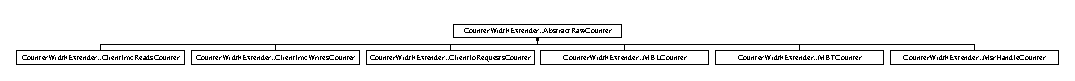
\includegraphics[height=0.645905cm]{struct_counter_width_extender_1_1_abstract_raw_counter}
\end{center}
\end{figure}
\subsection*{Public Member Functions}
\begin{DoxyCompactItemize}
\item 
\mbox{\Hypertarget{struct_counter_width_extender_1_1_abstract_raw_counter_a608ae097b3e1fd42768f3cd408fa123d}\label{struct_counter_width_extender_1_1_abstract_raw_counter_a608ae097b3e1fd42768f3cd408fa123d}} 
virtual uint64 {\bfseries operator()} ()=0
\end{DoxyCompactItemize}


The documentation for this struct was generated from the following file\+:\begin{DoxyCompactItemize}
\item 
\mbox{\hyperlink{width__extender_8h}{width\+\_\+extender.\+h}}\end{DoxyCompactItemize}

\hypertarget{class_asynchron_counter_state}{}\section{Asynchron\+Counter\+State Class Reference}
\label{class_asynchron_counter_state}\index{Asynchron\+Counter\+State@{Asynchron\+Counter\+State}}
\subsection*{Public Member Functions}
\begin{DoxyCompactItemize}
\item 
\mbox{\Hypertarget{class_asynchron_counter_state_ae50ebd3674b3ba52ff25f46b4eeb3956}\label{class_asynchron_counter_state_ae50ebd3674b3ba52ff25f46b4eeb3956}} 
uint32 {\bfseries get\+Num\+Cores} ()
\item 
\mbox{\Hypertarget{class_asynchron_counter_state_aad5f8ed144ee05d32c4b82e8664ea294}\label{class_asynchron_counter_state_aad5f8ed144ee05d32c4b82e8664ea294}} 
uint32 {\bfseries get\+Num\+Sockets} ()
\item 
\mbox{\Hypertarget{class_asynchron_counter_state_ab221a101212adceb2a248691eca8db1a}\label{class_asynchron_counter_state_ab221a101212adceb2a248691eca8db1a}} 
uint32 {\bfseries get\+Q\+P\+I\+Links\+Per\+Socket} ()
\item 
\mbox{\Hypertarget{class_asynchron_counter_state_a9121ce142b39fd845f6c4eb101c214bf}\label{class_asynchron_counter_state_a9121ce142b39fd845f6c4eb101c214bf}} 
uint32 {\bfseries get\+Socket\+Id} (uint32 c)
\item 
\mbox{\Hypertarget{class_asynchron_counter_state_a8f8e4539b38c5f171faa235b196e6f6a}\label{class_asynchron_counter_state_a8f8e4539b38c5f171faa235b196e6f6a}} 
{\footnotesize template$<$typename T , T  func$>$ }\\\mbox{\hyperlink{struct_t}{T}} {\bfseries get} (uint32 core)
\item 
\mbox{\Hypertarget{class_asynchron_counter_state_a8f8e4539b38c5f171faa235b196e6f6a}\label{class_asynchron_counter_state_a8f8e4539b38c5f171faa235b196e6f6a}} 
{\footnotesize template$<$typename T , T  func$>$ }\\\mbox{\hyperlink{struct_t}{T}} {\bfseries get} (uint32 core)
\item 
\mbox{\Hypertarget{class_asynchron_counter_state_aa77c2086bbaa8214dc60176f6ba08e43}\label{class_asynchron_counter_state_aa77c2086bbaa8214dc60176f6ba08e43}} 
{\footnotesize template$<$typename T , T  func$>$ }\\\mbox{\hyperlink{struct_t}{T}} {\bfseries get} (int param, uint32 core)
\item 
\mbox{\Hypertarget{class_asynchron_counter_state_a272fad1f3bd704f873c9c3a29e95192b}\label{class_asynchron_counter_state_a272fad1f3bd704f873c9c3a29e95192b}} 
{\footnotesize template$<$typename T , T  func$>$ }\\\mbox{\hyperlink{struct_t}{T}} {\bfseries get\+Socket} (uint32 socket)
\item 
\mbox{\Hypertarget{class_asynchron_counter_state_a272fad1f3bd704f873c9c3a29e95192b}\label{class_asynchron_counter_state_a272fad1f3bd704f873c9c3a29e95192b}} 
{\footnotesize template$<$typename T , T  func$>$ }\\\mbox{\hyperlink{struct_t}{T}} {\bfseries get\+Socket} (uint32 socket)
\item 
\mbox{\Hypertarget{class_asynchron_counter_state_aba3224acb89e692bb7024c85a516b8cb}\label{class_asynchron_counter_state_aba3224acb89e692bb7024c85a516b8cb}} 
{\footnotesize template$<$typename T , T  func$>$ }\\\mbox{\hyperlink{struct_t}{T}} {\bfseries get\+Socket} (int param, uint32 socket)
\item 
\mbox{\Hypertarget{class_asynchron_counter_state_ac5441bad9ff3aaccbe5b3b8965e091d2}\label{class_asynchron_counter_state_ac5441bad9ff3aaccbe5b3b8965e091d2}} 
{\footnotesize template$<$typename T , T  func$>$ }\\\mbox{\hyperlink{struct_t}{T}} {\bfseries get\+Socket} (uint32 socket, uint32 param)
\item 
\mbox{\Hypertarget{class_asynchron_counter_state_aa474d444ebe77a8c7e94c904e87879ae}\label{class_asynchron_counter_state_aa474d444ebe77a8c7e94c904e87879ae}} 
{\footnotesize template$<$typename T , T  func$>$ }\\\mbox{\hyperlink{struct_t}{T}} {\bfseries get\+System} ()
\item 
\mbox{\Hypertarget{class_asynchron_counter_state_a689f439c1e0f3b68401a0dd4341b46f0}\label{class_asynchron_counter_state_a689f439c1e0f3b68401a0dd4341b46f0}} 
{\footnotesize template$<$typename T , T  func$>$ }\\\mbox{\hyperlink{struct_t}{T}} {\bfseries get\+System} (int param)
\end{DoxyCompactItemize}
\subsection*{Friends}
\begin{DoxyCompactItemize}
\item 
\mbox{\Hypertarget{class_asynchron_counter_state_a972a576e955b250f38283c8c165a6c7a}\label{class_asynchron_counter_state_a972a576e955b250f38283c8c165a6c7a}} 
void $\ast$ {\bfseries Update\+Counters} (void $\ast$)
\end{DoxyCompactItemize}


The documentation for this class was generated from the following file\+:\begin{DoxyCompactItemize}
\item 
\mbox{\hyperlink{cpuasynchcounter_8h}{cpuasynchcounter.\+h}}\end{DoxyCompactItemize}

\hypertarget{class_basic_counter_state}{}\section{Basic\+Counter\+State Class Reference}
\label{class_basic_counter_state}\index{Basic\+Counter\+State@{Basic\+Counter\+State}}


Basic core counter state.  




{\ttfamily \#include $<$cpucounters.\+h$>$}

Inheritance diagram for Basic\+Counter\+State\+:\begin{figure}[H]
\begin{center}
\leavevmode
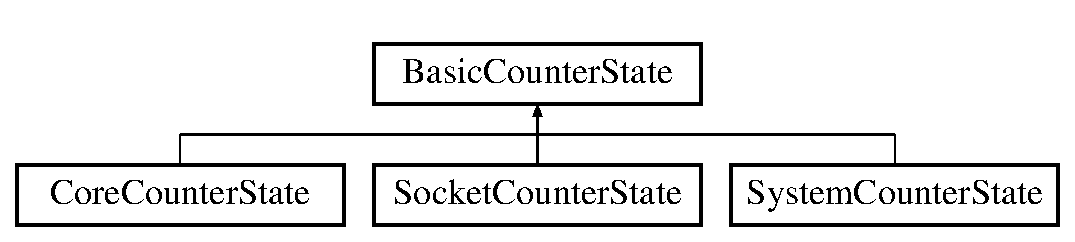
\includegraphics[height=2.000000cm]{class_basic_counter_state}
\end{center}
\end{figure}
\subsection*{Public Member Functions}
\begin{DoxyCompactItemize}
\item 
\mbox{\Hypertarget{class_basic_counter_state_a448f898e8ff78336611db856aa1354db}\label{class_basic_counter_state_a448f898e8ff78336611db856aa1354db}} 
\mbox{\hyperlink{class_basic_counter_state}{Basic\+Counter\+State}} \& {\bfseries operator+=} (const \mbox{\hyperlink{class_basic_counter_state}{Basic\+Counter\+State}} \&o)
\item 
\mbox{\Hypertarget{class_basic_counter_state_a57d93ca07fed611468739280015a3448}\label{class_basic_counter_state_a57d93ca07fed611468739280015a3448}} 
int32 \mbox{\hyperlink{class_basic_counter_state_a57d93ca07fed611468739280015a3448}{get\+Thermal\+Headroom}} () const
\begin{DoxyCompactList}\small\item\em Returns current thermal headroom below Tj\+Max. \end{DoxyCompactList}\end{DoxyCompactItemize}
\subsection*{Protected Member Functions}
\begin{DoxyCompactItemize}
\item 
\mbox{\Hypertarget{class_basic_counter_state_ae40030f6dc67badf91e4084397f998be}\label{class_basic_counter_state_ae40030f6dc67badf91e4084397f998be}} 
void {\bfseries read\+And\+Aggregate} (std\+::shared\+\_\+ptr$<$ \mbox{\hyperlink{class_safe_msr_handle}{Safe\+Msr\+Handle}} $>$)
\item 
\mbox{\Hypertarget{class_basic_counter_state_acb3ee2eabe21674e7930b19ef7ab3183}\label{class_basic_counter_state_acb3ee2eabe21674e7930b19ef7ab3183}} 
void {\bfseries read\+And\+Aggregate\+T\+SC} (std\+::shared\+\_\+ptr$<$ \mbox{\hyperlink{class_safe_msr_handle}{Safe\+Msr\+Handle}} $>$)
\end{DoxyCompactItemize}
\subsection*{Protected Attributes}
\begin{DoxyCompactItemize}
\item 
\mbox{\Hypertarget{class_basic_counter_state_a32d89649ba3e48ad8d0cfe05b0e5e2fb}\label{class_basic_counter_state_a32d89649ba3e48ad8d0cfe05b0e5e2fb}} 
uint64 {\bfseries Inst\+Retired\+Any}
\item 
\mbox{\Hypertarget{class_basic_counter_state_aa55976b14e3f5d61eac958ea5f80f35c}\label{class_basic_counter_state_aa55976b14e3f5d61eac958ea5f80f35c}} 
uint64 {\bfseries Cpu\+Clk\+Unhalted\+Thread}
\item 
\mbox{\Hypertarget{class_basic_counter_state_a9c64ac8f2c735b0a693a066ff99b9bc1}\label{class_basic_counter_state_a9c64ac8f2c735b0a693a066ff99b9bc1}} 
uint64 {\bfseries Cpu\+Clk\+Unhalted\+Ref}
\item 
\mbox{\Hypertarget{class_basic_counter_state_a9c856f4d132a302df428e99c817091ee}\label{class_basic_counter_state_a9c856f4d132a302df428e99c817091ee}} 
\begin{tabbing}
xx\=xx\=xx\=xx\=xx\=xx\=xx\=xx\=xx\=\kill
union \{\\
\>uint64 {\bfseries L3Miss}\\
\>uint64 {\bfseries Event0}\\
\>uint64 {\bfseries ArchLLCMiss}\\
\}; \\

\end{tabbing}\item 
\mbox{\Hypertarget{class_basic_counter_state_aa6cccd8d4cc29533223ceefd67d6aa36}\label{class_basic_counter_state_aa6cccd8d4cc29533223ceefd67d6aa36}} 
\begin{tabbing}
xx\=xx\=xx\=xx\=xx\=xx\=xx\=xx\=xx\=\kill
union \{\\
\>uint64 {\bfseries L3UnsharedHit}\\
\>uint64 {\bfseries Event1}\\
\>uint64 {\bfseries ArchLLCRef}\\
\>uint64 {\bfseries SKLL3Hit}\\
\}; \\

\end{tabbing}\item 
\mbox{\Hypertarget{class_basic_counter_state_a462224d3abe90b0d919dbd3862e8b82d}\label{class_basic_counter_state_a462224d3abe90b0d919dbd3862e8b82d}} 
\begin{tabbing}
xx\=xx\=xx\=xx\=xx\=xx\=xx\=xx\=xx\=\kill
union \{\\
\>uint64 {\bfseries L2HitM}\\
\>uint64 {\bfseries Event2}\\
\>uint64 {\bfseries SKLL2Miss}\\
\}; \\

\end{tabbing}\item 
\mbox{\Hypertarget{class_basic_counter_state_a8ad8f0451a153180e8e08ceb4c665ba2}\label{class_basic_counter_state_a8ad8f0451a153180e8e08ceb4c665ba2}} 
\begin{tabbing}
xx\=xx\=xx\=xx\=xx\=xx\=xx\=xx\=xx\=\kill
union \{\\
\>uint64 {\bfseries L2Hit}\\
\>uint64 {\bfseries Event3}\\
\}; \\

\end{tabbing}\item 
\mbox{\Hypertarget{class_basic_counter_state_af357162e5b43c6dfc0ce92fd56fa30a0}\label{class_basic_counter_state_af357162e5b43c6dfc0ce92fd56fa30a0}} 
uint64 {\bfseries Invariant\+T\+SC}
\item 
\mbox{\Hypertarget{class_basic_counter_state_af9069c972052bac5ed648e519e03da9c}\label{class_basic_counter_state_af9069c972052bac5ed648e519e03da9c}} 
uint64 {\bfseries C\+State\+Residency} \mbox{[}P\+C\+M\+::\+M\+A\+X\+\_\+\+C\+\_\+\+S\+T\+A\+TE+1\mbox{]}
\item 
\mbox{\Hypertarget{class_basic_counter_state_a4950fe3761b2ac599a7ae64ec7bee973}\label{class_basic_counter_state_a4950fe3761b2ac599a7ae64ec7bee973}} 
int32 {\bfseries Thermal\+Headroom}
\item 
\mbox{\Hypertarget{class_basic_counter_state_a99dab23e20418b86be72dda1ecd8858c}\label{class_basic_counter_state_a99dab23e20418b86be72dda1ecd8858c}} 
uint64 {\bfseries L3\+Occupancy}
\item 
\mbox{\Hypertarget{class_basic_counter_state_a115320ce0518d55acd0db90c127419b8}\label{class_basic_counter_state_a115320ce0518d55acd0db90c127419b8}} 
uint64 {\bfseries Memory\+B\+W\+Local}
\item 
\mbox{\Hypertarget{class_basic_counter_state_a97a5bc9ad3dc45a876a34740537e54a8}\label{class_basic_counter_state_a97a5bc9ad3dc45a876a34740537e54a8}} 
uint64 {\bfseries Memory\+B\+W\+Total}
\item 
\mbox{\Hypertarget{class_basic_counter_state_a1776fe74136c0e204c68885f23989828}\label{class_basic_counter_state_a1776fe74136c0e204c68885f23989828}} 
uint64 {\bfseries S\+M\+I\+Count}
\end{DoxyCompactItemize}
\subsection*{Friends}
\begin{DoxyCompactItemize}
\item 
\mbox{\Hypertarget{class_basic_counter_state_ab5f56d2e95ba3daf52c17b8a1d356d64}\label{class_basic_counter_state_ab5f56d2e95ba3daf52c17b8a1d356d64}} 
class {\bfseries P\+CM}
\item 
{\footnotesize template$<$class Counter\+State\+Type $>$ }\\double \mbox{\hyperlink{class_basic_counter_state_a159a6896f5ef3626b88cdd27a3c15ac0}{get\+Exec\+Usage}} (const Counter\+State\+Type \&before, const Counter\+State\+Type \&after)
\begin{DoxyCompactList}\small\item\em Computes average number of retired instructions per time intervall. \end{DoxyCompactList}\item 
{\footnotesize template$<$class Counter\+State\+Type $>$ }\\double \mbox{\hyperlink{class_basic_counter_state_a7b0019d24a77dc05b7e47cb98192fd22}{get\+I\+PC}} (const Counter\+State\+Type \&before, const Counter\+State\+Type \&after)
\begin{DoxyCompactList}\small\item\em Computes average number of retired instructions per core cycle (I\+PC) \end{DoxyCompactList}\item 
{\footnotesize template$<$class Counter\+State\+Type $>$ }\\double \mbox{\hyperlink{class_basic_counter_state_aa398facfd523b7dcdbf827a74970a88c}{get\+Average\+Frequency}} (const Counter\+State\+Type \&before, const Counter\+State\+Type \&after)
\begin{DoxyCompactList}\small\item\em Computes average core frequency also taking Intel Turbo Boost technology into account. \end{DoxyCompactList}\item 
{\footnotesize template$<$class Counter\+State\+Type $>$ }\\double \mbox{\hyperlink{class_basic_counter_state_a963d78be64ccddb4f7686405ef4df9c1}{get\+Active\+Average\+Frequency}} (const Counter\+State\+Type \&before, const Counter\+State\+Type \&after)
\begin{DoxyCompactList}\small\item\em Computes average core frequency when not in powersaving C0-\/state (also taking Intel Turbo Boost technology into account) \end{DoxyCompactList}\item 
{\footnotesize template$<$class Counter\+State\+Type $>$ }\\double \mbox{\hyperlink{class_basic_counter_state_a806e72bc51f05acc4af0667ca3334242}{get\+Relative\+Frequency}} (const Counter\+State\+Type \&before, const Counter\+State\+Type \&after)
\begin{DoxyCompactList}\small\item\em Computes average core frequency also taking Intel Turbo Boost technology into account. \end{DoxyCompactList}\item 
{\footnotesize template$<$class Counter\+State\+Type $>$ }\\double \mbox{\hyperlink{class_basic_counter_state_a9a351e598b8af26131611ff37b592633}{get\+Active\+Relative\+Frequency}} (const Counter\+State\+Type \&before, const Counter\+State\+Type \&after)
\begin{DoxyCompactList}\small\item\em Computes average core frequency when not in powersaving C0-\/state (also taking Intel Turbo Boost technology into account) \end{DoxyCompactList}\item 
{\footnotesize template$<$class Counter\+State\+Type $>$ }\\double \mbox{\hyperlink{class_basic_counter_state_a5922acedeec3c1cc67d20670f8ef0518}{get\+L2\+Cache\+Hit\+Ratio}} (const Counter\+State\+Type \&before, const Counter\+State\+Type \&after)
\begin{DoxyCompactList}\small\item\em Computes L2 cache hit ratio. \end{DoxyCompactList}\item 
{\footnotesize template$<$class Counter\+State\+Type $>$ }\\double \mbox{\hyperlink{class_basic_counter_state_a7b03f0cd02862716d717e897032b7885}{get\+L3\+Cache\+Hit\+Ratio}} (const Counter\+State\+Type \&before, const Counter\+State\+Type \&after)
\begin{DoxyCompactList}\small\item\em Computes L3 cache hit ratio. \end{DoxyCompactList}\item 
{\footnotesize template$<$class Counter\+State\+Type $>$ }\\uint64 \mbox{\hyperlink{class_basic_counter_state_a94118e70266db2ed7fc6b8b7b4e2c343}{get\+L3\+Cache\+Misses}} (const Counter\+State\+Type \&before, const Counter\+State\+Type \&after)
\begin{DoxyCompactList}\small\item\em Computes number of L3 cache misses. \end{DoxyCompactList}\item 
{\footnotesize template$<$class Counter\+State\+Type $>$ }\\uint64 \mbox{\hyperlink{class_basic_counter_state_a291eeab262fdb93de08cdfdf50dbad58}{get\+L2\+Cache\+Misses}} (const Counter\+State\+Type \&before, const Counter\+State\+Type \&after)
\begin{DoxyCompactList}\small\item\em Computes number of L2 cache misses. \end{DoxyCompactList}\item 
{\footnotesize template$<$class Counter\+State\+Type $>$ }\\uint64 \mbox{\hyperlink{class_basic_counter_state_a459367d7877d09594c2ecd85e04cae61}{get\+L2\+Cache\+Hits}} (const Counter\+State\+Type \&before, const Counter\+State\+Type \&after)
\begin{DoxyCompactList}\small\item\em Computes number of L2 cache hits. \end{DoxyCompactList}\item 
{\footnotesize template$<$class Counter\+State\+Type $>$ }\\uint64 \mbox{\hyperlink{class_basic_counter_state_ace0e3ffc23c20d0eda7663cb7e4899a2}{get\+L3\+Cache\+Hits\+No\+Snoop}} (const Counter\+State\+Type \&before, const Counter\+State\+Type \&after)
\begin{DoxyCompactList}\small\item\em Computes number of L3 cache hits where no snooping in sibling L2 caches had to be done. \end{DoxyCompactList}\item 
{\footnotesize template$<$class Counter\+State\+Type $>$ }\\uint64 \mbox{\hyperlink{class_basic_counter_state_a4b1050ca9ccdd66661df556bab70fd0f}{get\+L3\+Cache\+Hits\+Snoop}} (const Counter\+State\+Type \&before, const Counter\+State\+Type \&after)
\begin{DoxyCompactList}\small\item\em Computes number of L3 cache hits where snooping in sibling L2 caches had to be done. \end{DoxyCompactList}\item 
{\footnotesize template$<$class Counter\+State\+Type $>$ }\\uint64 \mbox{\hyperlink{class_basic_counter_state_a7ba16714ef7ed547ad8648cb5b9e52f6}{get\+L3\+Cache\+Hits}} (const Counter\+State\+Type \&before, const Counter\+State\+Type \&after)
\begin{DoxyCompactList}\small\item\em Computes total number of L3 cache hits. \end{DoxyCompactList}\item 
{\footnotesize template$<$class Counter\+State\+Type $>$ }\\double \mbox{\hyperlink{class_basic_counter_state_a89d4cef9c83db7e76be6a0a2e7351e2e}{get\+Cycles\+Lost\+Due\+L3\+Cache\+Misses}} (const Counter\+State\+Type \&before, const Counter\+State\+Type \&after)
\begin{DoxyCompactList}\small\item\em Estimates how many core cycles were potentially lost due to L3 cache misses. \end{DoxyCompactList}\item 
{\footnotesize template$<$class Counter\+State\+Type $>$ }\\double \mbox{\hyperlink{class_basic_counter_state_ac26765efe8a4c7341f40c8ab8bdb9af6}{get\+Cycles\+Lost\+Due\+L2\+Cache\+Misses}} (const Counter\+State\+Type \&before, const Counter\+State\+Type \&after)
\begin{DoxyCompactList}\small\item\em Estimates how many core cycles were potentially lost due to missing L2 cache but still hitting L3 cache. \end{DoxyCompactList}\item 
{\footnotesize template$<$class Counter\+State\+Type $>$ }\\uint64 \mbox{\hyperlink{class_basic_counter_state_a185f850a9a753d9cf4deb8299261fd4c}{get\+L3\+Cache\+Occupancy}} (const Counter\+State\+Type \&now)
\begin{DoxyCompactList}\small\item\em Computes L3 Cache Occupancy. \end{DoxyCompactList}\item 
{\footnotesize template$<$class Counter\+State\+Type $>$ }\\uint64 \mbox{\hyperlink{class_basic_counter_state_a3ba7c9267c6e0f338a59defc98ae0007}{get\+Local\+Memory\+BW}} (const Counter\+State\+Type \&before, const Counter\+State\+Type \&after)
\begin{DoxyCompactList}\small\item\em Computes Local Memory Bandwidth. \end{DoxyCompactList}\item 
{\footnotesize template$<$class Counter\+State\+Type $>$ }\\uint64 \mbox{\hyperlink{class_basic_counter_state_a00c97b1a7d8a7125ce7fd129cddb52e8}{get\+Remote\+Memory\+BW}} (const Counter\+State\+Type \&before, const Counter\+State\+Type \&after)
\begin{DoxyCompactList}\small\item\em Computes Remote Memory Bandwidth. \end{DoxyCompactList}\item 
{\footnotesize template$<$class Counter\+State\+Type $>$ }\\uint64 \mbox{\hyperlink{class_basic_counter_state_a5a3275c4f489a475f1658f4546567af4}{get\+Cycles}} (const Counter\+State\+Type \&before, const Counter\+State\+Type \&after)
\begin{DoxyCompactList}\small\item\em Computes the number core clock cycles when signal on a specific core is running (not halted) \end{DoxyCompactList}\item 
{\footnotesize template$<$class Counter\+State\+Type $>$ }\\uint64 \mbox{\hyperlink{class_basic_counter_state_af124718a7620c7bbca81232c2149f771}{get\+Instructions\+Retired}} (const Counter\+State\+Type \&before, const Counter\+State\+Type \&after)
\begin{DoxyCompactList}\small\item\em Computes the number of retired instructions. \end{DoxyCompactList}\item 
{\footnotesize template$<$class Counter\+State\+Type $>$ }\\uint64 \mbox{\hyperlink{class_basic_counter_state_adc17d576ecaf02cf98cebc86329bf2a1}{get\+Cycles}} (const Counter\+State\+Type \&now)
\begin{DoxyCompactList}\small\item\em Computes the number executed core clock cycles. \end{DoxyCompactList}\item 
{\footnotesize template$<$class Counter\+State\+Type $>$ }\\uint64 \mbox{\hyperlink{class_basic_counter_state_afced47e4bb3712da79dc64cb16ac335a}{get\+Instructions\+Retired}} (const Counter\+State\+Type \&now)
\begin{DoxyCompactList}\small\item\em Computes the number of retired instructions. \end{DoxyCompactList}\item 
{\footnotesize template$<$class Counter\+State\+Type $>$ }\\uint64 \mbox{\hyperlink{class_basic_counter_state_abaa9d828b52f41866bf7dc8ff491a62e}{get\+Number\+Of\+Custom\+Events}} (int32 event\+Counter\+Nr, const Counter\+State\+Type \&before, const Counter\+State\+Type \&after)
\begin{DoxyCompactList}\small\item\em Returns the number of occured custom core events. \end{DoxyCompactList}\item 
{\footnotesize template$<$class Counter\+State\+Type $>$ }\\uint64 \mbox{\hyperlink{class_basic_counter_state_a45cf07a8d3ce2c48968842554a3854f9}{get\+Invariant\+T\+SC}} (const Counter\+State\+Type \&before, const Counter\+State\+Type \&after)
\begin{DoxyCompactList}\small\item\em Computes number of invariant time stamp counter ticks. \end{DoxyCompactList}\item 
{\footnotesize template$<$class Counter\+State\+Type $>$ }\\uint64 \mbox{\hyperlink{class_basic_counter_state_aaa3691b803702deec828d0d8d8a8f326}{get\+Ref\+Cycles}} (const Counter\+State\+Type \&before, const Counter\+State\+Type \&after)
\begin{DoxyCompactList}\small\item\em Computes the number of reference clock cycles while clock signal on the core is running. \end{DoxyCompactList}\item 
{\footnotesize template$<$class Counter\+State\+Type $>$ }\\double \mbox{\hyperlink{class_basic_counter_state_a98aa8d4eb21e8a992fc181d65018e5ce}{get\+Core\+C\+State\+Residency}} (int state, const Counter\+State\+Type \&before, const Counter\+State\+Type \&after)
\begin{DoxyCompactList}\small\item\em Computes residency in the core C-\/state. \end{DoxyCompactList}\item 
{\footnotesize template$<$class Counter\+State\+Type $>$ }\\uint64 \mbox{\hyperlink{class_basic_counter_state_a5e245473e2297272a50ca054b33c8c86}{get\+S\+M\+I\+Count}} (const Counter\+State\+Type \&before, const Counter\+State\+Type \&after)
\begin{DoxyCompactList}\small\item\em Returns the number of occured system management interrupts. \end{DoxyCompactList}\end{DoxyCompactItemize}


\subsection{Detailed Description}
Basic core counter state. 

Intended only for derivation, but not for the direct use 

\subsection{Friends And Related Function Documentation}
\mbox{\Hypertarget{class_basic_counter_state_a963d78be64ccddb4f7686405ef4df9c1}\label{class_basic_counter_state_a963d78be64ccddb4f7686405ef4df9c1}} 
\index{Basic\+Counter\+State@{Basic\+Counter\+State}!get\+Active\+Average\+Frequency@{get\+Active\+Average\+Frequency}}
\index{get\+Active\+Average\+Frequency@{get\+Active\+Average\+Frequency}!Basic\+Counter\+State@{Basic\+Counter\+State}}
\subsubsection{\texorpdfstring{get\+Active\+Average\+Frequency}{getActiveAverageFrequency}}
{\footnotesize\ttfamily template$<$class Counter\+State\+Type $>$ \\
double get\+Active\+Average\+Frequency (\begin{DoxyParamCaption}\item[{const Counter\+State\+Type \&}]{before,  }\item[{const Counter\+State\+Type \&}]{after }\end{DoxyParamCaption})\hspace{0.3cm}{\ttfamily [friend]}}



Computes average core frequency when not in powersaving C0-\/state (also taking Intel Turbo Boost technology into account) 


\begin{DoxyParams}{Parameters}
{\em before} & C\+PU counter state before the experiment \\
\hline
{\em after} & C\+PU counter state after the experiment \\
\hline
\end{DoxyParams}
\begin{DoxyReturn}{Returns}
frequency in Hz 
\end{DoxyReturn}
\mbox{\Hypertarget{class_basic_counter_state_a9a351e598b8af26131611ff37b592633}\label{class_basic_counter_state_a9a351e598b8af26131611ff37b592633}} 
\index{Basic\+Counter\+State@{Basic\+Counter\+State}!get\+Active\+Relative\+Frequency@{get\+Active\+Relative\+Frequency}}
\index{get\+Active\+Relative\+Frequency@{get\+Active\+Relative\+Frequency}!Basic\+Counter\+State@{Basic\+Counter\+State}}
\subsubsection{\texorpdfstring{get\+Active\+Relative\+Frequency}{getActiveRelativeFrequency}}
{\footnotesize\ttfamily template$<$class Counter\+State\+Type $>$ \\
double get\+Active\+Relative\+Frequency (\begin{DoxyParamCaption}\item[{const Counter\+State\+Type \&}]{before,  }\item[{const Counter\+State\+Type \&}]{after }\end{DoxyParamCaption})\hspace{0.3cm}{\ttfamily [friend]}}



Computes average core frequency when not in powersaving C0-\/state (also taking Intel Turbo Boost technology into account) 


\begin{DoxyParams}{Parameters}
{\em before} & C\+PU counter state before the experiment \\
\hline
{\em after} & C\+PU counter state after the experiment \\
\hline
\end{DoxyParams}
\begin{DoxyReturn}{Returns}
Fraction of nominal frequency (if $>$1.\+0 then Turbo was working during the measurement) 
\end{DoxyReturn}
\mbox{\Hypertarget{class_basic_counter_state_aa398facfd523b7dcdbf827a74970a88c}\label{class_basic_counter_state_aa398facfd523b7dcdbf827a74970a88c}} 
\index{Basic\+Counter\+State@{Basic\+Counter\+State}!get\+Average\+Frequency@{get\+Average\+Frequency}}
\index{get\+Average\+Frequency@{get\+Average\+Frequency}!Basic\+Counter\+State@{Basic\+Counter\+State}}
\subsubsection{\texorpdfstring{get\+Average\+Frequency}{getAverageFrequency}}
{\footnotesize\ttfamily template$<$class Counter\+State\+Type $>$ \\
double get\+Average\+Frequency (\begin{DoxyParamCaption}\item[{const Counter\+State\+Type \&}]{before,  }\item[{const Counter\+State\+Type \&}]{after }\end{DoxyParamCaption})\hspace{0.3cm}{\ttfamily [friend]}}



Computes average core frequency also taking Intel Turbo Boost technology into account. 


\begin{DoxyParams}{Parameters}
{\em before} & C\+PU counter state before the experiment \\
\hline
{\em after} & C\+PU counter state after the experiment \\
\hline
\end{DoxyParams}
\begin{DoxyReturn}{Returns}
frequency in Hz 
\end{DoxyReturn}
\mbox{\Hypertarget{class_basic_counter_state_a98aa8d4eb21e8a992fc181d65018e5ce}\label{class_basic_counter_state_a98aa8d4eb21e8a992fc181d65018e5ce}} 
\index{Basic\+Counter\+State@{Basic\+Counter\+State}!get\+Core\+C\+State\+Residency@{get\+Core\+C\+State\+Residency}}
\index{get\+Core\+C\+State\+Residency@{get\+Core\+C\+State\+Residency}!Basic\+Counter\+State@{Basic\+Counter\+State}}
\subsubsection{\texorpdfstring{get\+Core\+C\+State\+Residency}{getCoreCStateResidency}}
{\footnotesize\ttfamily template$<$class Counter\+State\+Type $>$ \\
double get\+Core\+C\+State\+Residency (\begin{DoxyParamCaption}\item[{int}]{state,  }\item[{const Counter\+State\+Type \&}]{before,  }\item[{const Counter\+State\+Type \&}]{after }\end{DoxyParamCaption})\hspace{0.3cm}{\ttfamily [friend]}}



Computes residency in the core C-\/state. 


\begin{DoxyParams}{Parameters}
{\em state} & C-\/state \\
\hline
{\em before} & C\+PU counter state before the experiment \\
\hline
{\em after} & C\+PU counter state after the experiment \\
\hline
\end{DoxyParams}
\begin{DoxyReturn}{Returns}
residence ratio (0..1)\+: 0 -\/ 0\%, 1.\+0 -\/ 100\% 
\end{DoxyReturn}
\mbox{\Hypertarget{class_basic_counter_state_a5a3275c4f489a475f1658f4546567af4}\label{class_basic_counter_state_a5a3275c4f489a475f1658f4546567af4}} 
\index{Basic\+Counter\+State@{Basic\+Counter\+State}!get\+Cycles@{get\+Cycles}}
\index{get\+Cycles@{get\+Cycles}!Basic\+Counter\+State@{Basic\+Counter\+State}}
\subsubsection{\texorpdfstring{get\+Cycles}{getCycles}\hspace{0.1cm}{\footnotesize\ttfamily [1/2]}}
{\footnotesize\ttfamily template$<$class Counter\+State\+Type $>$ \\
uint64 get\+Cycles (\begin{DoxyParamCaption}\item[{const Counter\+State\+Type \&}]{before,  }\item[{const Counter\+State\+Type \&}]{after }\end{DoxyParamCaption})\hspace{0.3cm}{\ttfamily [friend]}}



Computes the number core clock cycles when signal on a specific core is running (not halted) 

Returns number of used cycles (halted cyles are not counted). The counter does not advance in the following conditions\+:
\begin{DoxyItemize}
\item an A\+C\+PI C-\/state is other than C0 for normal operation
\item H\+LT
\item S\+T\+P\+C\+L\+K+ pin is asserted
\item being throttled by T\+M1
\item during the frequency switching phase of a performance state transition
\end{DoxyItemize}

The performance counter for this event counts across performance state transitions using different core clock frequencies


\begin{DoxyParams}{Parameters}
{\em before} & C\+PU counter state before the experiment \\
\hline
{\em after} & C\+PU counter state after the experiment \\
\hline
\end{DoxyParams}
\begin{DoxyReturn}{Returns}
number core clock cycles 
\end{DoxyReturn}
\mbox{\Hypertarget{class_basic_counter_state_adc17d576ecaf02cf98cebc86329bf2a1}\label{class_basic_counter_state_adc17d576ecaf02cf98cebc86329bf2a1}} 
\index{Basic\+Counter\+State@{Basic\+Counter\+State}!get\+Cycles@{get\+Cycles}}
\index{get\+Cycles@{get\+Cycles}!Basic\+Counter\+State@{Basic\+Counter\+State}}
\subsubsection{\texorpdfstring{get\+Cycles}{getCycles}\hspace{0.1cm}{\footnotesize\ttfamily [2/2]}}
{\footnotesize\ttfamily template$<$class Counter\+State\+Type $>$ \\
uint64 get\+Cycles (\begin{DoxyParamCaption}\item[{const Counter\+State\+Type \&}]{now }\end{DoxyParamCaption})\hspace{0.3cm}{\ttfamily [friend]}}



Computes the number executed core clock cycles. 

Returns number of used cycles (halted cyles are not counted).


\begin{DoxyParams}{Parameters}
{\em now} & Current C\+PU counter state \\
\hline
\end{DoxyParams}
\begin{DoxyReturn}{Returns}
number core clock cycles 
\end{DoxyReturn}
\mbox{\Hypertarget{class_basic_counter_state_ac26765efe8a4c7341f40c8ab8bdb9af6}\label{class_basic_counter_state_ac26765efe8a4c7341f40c8ab8bdb9af6}} 
\index{Basic\+Counter\+State@{Basic\+Counter\+State}!get\+Cycles\+Lost\+Due\+L2\+Cache\+Misses@{get\+Cycles\+Lost\+Due\+L2\+Cache\+Misses}}
\index{get\+Cycles\+Lost\+Due\+L2\+Cache\+Misses@{get\+Cycles\+Lost\+Due\+L2\+Cache\+Misses}!Basic\+Counter\+State@{Basic\+Counter\+State}}
\subsubsection{\texorpdfstring{get\+Cycles\+Lost\+Due\+L2\+Cache\+Misses}{getCyclesLostDueL2CacheMisses}}
{\footnotesize\ttfamily template$<$class Counter\+State\+Type $>$ \\
double get\+Cycles\+Lost\+Due\+L2\+Cache\+Misses (\begin{DoxyParamCaption}\item[{const Counter\+State\+Type \&}]{before,  }\item[{const Counter\+State\+Type \&}]{after }\end{DoxyParamCaption})\hspace{0.3cm}{\ttfamily [friend]}}



Estimates how many core cycles were potentially lost due to missing L2 cache but still hitting L3 cache. 


\begin{DoxyParams}{Parameters}
{\em before} & C\+PU counter state before the experiment \\
\hline
{\em after} & C\+PU counter state after the experiment \\
\hline
\end{DoxyParams}
\begin{DoxyWarning}{Warning}
Works only in the D\+E\+F\+A\+U\+L\+T\+\_\+\+E\+V\+E\+N\+TS programming mode (see program() method) 

Currently not supported on Intel(\+R) Atom(tm) processor 
\end{DoxyWarning}
\begin{DoxyReturn}{Returns}
ratio that is usually beetween 0 and 1 ; in some cases could be $>$1.\+0 due to a lower access latency estimation 
\end{DoxyReturn}
\mbox{\Hypertarget{class_basic_counter_state_a89d4cef9c83db7e76be6a0a2e7351e2e}\label{class_basic_counter_state_a89d4cef9c83db7e76be6a0a2e7351e2e}} 
\index{Basic\+Counter\+State@{Basic\+Counter\+State}!get\+Cycles\+Lost\+Due\+L3\+Cache\+Misses@{get\+Cycles\+Lost\+Due\+L3\+Cache\+Misses}}
\index{get\+Cycles\+Lost\+Due\+L3\+Cache\+Misses@{get\+Cycles\+Lost\+Due\+L3\+Cache\+Misses}!Basic\+Counter\+State@{Basic\+Counter\+State}}
\subsubsection{\texorpdfstring{get\+Cycles\+Lost\+Due\+L3\+Cache\+Misses}{getCyclesLostDueL3CacheMisses}}
{\footnotesize\ttfamily template$<$class Counter\+State\+Type $>$ \\
double get\+Cycles\+Lost\+Due\+L3\+Cache\+Misses (\begin{DoxyParamCaption}\item[{const Counter\+State\+Type \&}]{before,  }\item[{const Counter\+State\+Type \&}]{after }\end{DoxyParamCaption})\hspace{0.3cm}{\ttfamily [friend]}}



Estimates how many core cycles were potentially lost due to L3 cache misses. 


\begin{DoxyParams}{Parameters}
{\em before} & C\+PU counter state before the experiment \\
\hline
{\em after} & C\+PU counter state after the experiment \\
\hline
\end{DoxyParams}
\begin{DoxyWarning}{Warning}
Works only in the D\+E\+F\+A\+U\+L\+T\+\_\+\+E\+V\+E\+N\+TS programming mode (see program() method) 
\end{DoxyWarning}
\begin{DoxyReturn}{Returns}
ratio that is usually beetween 0 and 1 ; in some cases could be $>$1.\+0 due to a lower memory latency estimation 
\end{DoxyReturn}
\mbox{\Hypertarget{class_basic_counter_state_a159a6896f5ef3626b88cdd27a3c15ac0}\label{class_basic_counter_state_a159a6896f5ef3626b88cdd27a3c15ac0}} 
\index{Basic\+Counter\+State@{Basic\+Counter\+State}!get\+Exec\+Usage@{get\+Exec\+Usage}}
\index{get\+Exec\+Usage@{get\+Exec\+Usage}!Basic\+Counter\+State@{Basic\+Counter\+State}}
\subsubsection{\texorpdfstring{get\+Exec\+Usage}{getExecUsage}}
{\footnotesize\ttfamily template$<$class Counter\+State\+Type $>$ \\
double get\+Exec\+Usage (\begin{DoxyParamCaption}\item[{const Counter\+State\+Type \&}]{before,  }\item[{const Counter\+State\+Type \&}]{after }\end{DoxyParamCaption})\hspace{0.3cm}{\ttfamily [friend]}}



Computes average number of retired instructions per time intervall. 


\begin{DoxyParams}{Parameters}
{\em before} & C\+PU counter state before the experiment \\
\hline
{\em after} & C\+PU counter state after the experiment \\
\hline
\end{DoxyParams}
\begin{DoxyReturn}{Returns}
usage 
\end{DoxyReturn}
\mbox{\Hypertarget{class_basic_counter_state_af124718a7620c7bbca81232c2149f771}\label{class_basic_counter_state_af124718a7620c7bbca81232c2149f771}} 
\index{Basic\+Counter\+State@{Basic\+Counter\+State}!get\+Instructions\+Retired@{get\+Instructions\+Retired}}
\index{get\+Instructions\+Retired@{get\+Instructions\+Retired}!Basic\+Counter\+State@{Basic\+Counter\+State}}
\subsubsection{\texorpdfstring{get\+Instructions\+Retired}{getInstructionsRetired}\hspace{0.1cm}{\footnotesize\ttfamily [1/2]}}
{\footnotesize\ttfamily template$<$class Counter\+State\+Type $>$ \\
uint64 get\+Instructions\+Retired (\begin{DoxyParamCaption}\item[{const Counter\+State\+Type \&}]{before,  }\item[{const Counter\+State\+Type \&}]{after }\end{DoxyParamCaption})\hspace{0.3cm}{\ttfamily [friend]}}



Computes the number of retired instructions. 


\begin{DoxyParams}{Parameters}
{\em before} & C\+PU counter state before the experiment \\
\hline
{\em after} & C\+PU counter state after the experiment \\
\hline
\end{DoxyParams}
\begin{DoxyReturn}{Returns}
number of retired instructions 
\end{DoxyReturn}
\mbox{\Hypertarget{class_basic_counter_state_afced47e4bb3712da79dc64cb16ac335a}\label{class_basic_counter_state_afced47e4bb3712da79dc64cb16ac335a}} 
\index{Basic\+Counter\+State@{Basic\+Counter\+State}!get\+Instructions\+Retired@{get\+Instructions\+Retired}}
\index{get\+Instructions\+Retired@{get\+Instructions\+Retired}!Basic\+Counter\+State@{Basic\+Counter\+State}}
\subsubsection{\texorpdfstring{get\+Instructions\+Retired}{getInstructionsRetired}\hspace{0.1cm}{\footnotesize\ttfamily [2/2]}}
{\footnotesize\ttfamily template$<$class Counter\+State\+Type $>$ \\
uint64 get\+Instructions\+Retired (\begin{DoxyParamCaption}\item[{const Counter\+State\+Type \&}]{now }\end{DoxyParamCaption})\hspace{0.3cm}{\ttfamily [friend]}}



Computes the number of retired instructions. 


\begin{DoxyParams}{Parameters}
{\em now} & Current C\+PU counter state \\
\hline
\end{DoxyParams}
\begin{DoxyReturn}{Returns}
number of retired instructions 
\end{DoxyReturn}
\mbox{\Hypertarget{class_basic_counter_state_a45cf07a8d3ce2c48968842554a3854f9}\label{class_basic_counter_state_a45cf07a8d3ce2c48968842554a3854f9}} 
\index{Basic\+Counter\+State@{Basic\+Counter\+State}!get\+Invariant\+T\+SC@{get\+Invariant\+T\+SC}}
\index{get\+Invariant\+T\+SC@{get\+Invariant\+T\+SC}!Basic\+Counter\+State@{Basic\+Counter\+State}}
\subsubsection{\texorpdfstring{get\+Invariant\+T\+SC}{getInvariantTSC}}
{\footnotesize\ttfamily template$<$class Counter\+State\+Type $>$ \\
uint64 get\+Invariant\+T\+SC (\begin{DoxyParamCaption}\item[{const Counter\+State\+Type \&}]{before,  }\item[{const Counter\+State\+Type \&}]{after }\end{DoxyParamCaption})\hspace{0.3cm}{\ttfamily [friend]}}



Computes number of invariant time stamp counter ticks. 

This counter counts irrespectively of C-\/, P-\/ or T-\/states


\begin{DoxyParams}{Parameters}
{\em before} & C\+PU counter state before the experiment \\
\hline
{\em after} & C\+PU counter state after the experiment \\
\hline
\end{DoxyParams}
\begin{DoxyReturn}{Returns}
number of time stamp counter ticks 
\end{DoxyReturn}
\mbox{\Hypertarget{class_basic_counter_state_a7b0019d24a77dc05b7e47cb98192fd22}\label{class_basic_counter_state_a7b0019d24a77dc05b7e47cb98192fd22}} 
\index{Basic\+Counter\+State@{Basic\+Counter\+State}!get\+I\+PC@{get\+I\+PC}}
\index{get\+I\+PC@{get\+I\+PC}!Basic\+Counter\+State@{Basic\+Counter\+State}}
\subsubsection{\texorpdfstring{get\+I\+PC}{getIPC}}
{\footnotesize\ttfamily template$<$class Counter\+State\+Type $>$ \\
double get\+I\+PC (\begin{DoxyParamCaption}\item[{const Counter\+State\+Type \&}]{before,  }\item[{const Counter\+State\+Type \&}]{after }\end{DoxyParamCaption})\hspace{0.3cm}{\ttfamily [friend]}}



Computes average number of retired instructions per core cycle (I\+PC) 


\begin{DoxyParams}{Parameters}
{\em before} & C\+PU counter state before the experiment \\
\hline
{\em after} & C\+PU counter state after the experiment \\
\hline
\end{DoxyParams}
\begin{DoxyReturn}{Returns}
I\+PC 
\end{DoxyReturn}
\mbox{\Hypertarget{class_basic_counter_state_a5922acedeec3c1cc67d20670f8ef0518}\label{class_basic_counter_state_a5922acedeec3c1cc67d20670f8ef0518}} 
\index{Basic\+Counter\+State@{Basic\+Counter\+State}!get\+L2\+Cache\+Hit\+Ratio@{get\+L2\+Cache\+Hit\+Ratio}}
\index{get\+L2\+Cache\+Hit\+Ratio@{get\+L2\+Cache\+Hit\+Ratio}!Basic\+Counter\+State@{Basic\+Counter\+State}}
\subsubsection{\texorpdfstring{get\+L2\+Cache\+Hit\+Ratio}{getL2CacheHitRatio}}
{\footnotesize\ttfamily template$<$class Counter\+State\+Type $>$ \\
double get\+L2\+Cache\+Hit\+Ratio (\begin{DoxyParamCaption}\item[{const Counter\+State\+Type \&}]{before,  }\item[{const Counter\+State\+Type \&}]{after }\end{DoxyParamCaption})\hspace{0.3cm}{\ttfamily [friend]}}



Computes L2 cache hit ratio. 


\begin{DoxyParams}{Parameters}
{\em before} & C\+PU counter state before the experiment \\
\hline
{\em after} & C\+PU counter state after the experiment \\
\hline
\end{DoxyParams}
\begin{DoxyWarning}{Warning}
Works only in the D\+E\+F\+A\+U\+L\+T\+\_\+\+E\+V\+E\+N\+TS programming mode (see program() method) 
\end{DoxyWarning}
\begin{DoxyReturn}{Returns}
value between 0 and 1 
\end{DoxyReturn}
\mbox{\Hypertarget{class_basic_counter_state_a459367d7877d09594c2ecd85e04cae61}\label{class_basic_counter_state_a459367d7877d09594c2ecd85e04cae61}} 
\index{Basic\+Counter\+State@{Basic\+Counter\+State}!get\+L2\+Cache\+Hits@{get\+L2\+Cache\+Hits}}
\index{get\+L2\+Cache\+Hits@{get\+L2\+Cache\+Hits}!Basic\+Counter\+State@{Basic\+Counter\+State}}
\subsubsection{\texorpdfstring{get\+L2\+Cache\+Hits}{getL2CacheHits}}
{\footnotesize\ttfamily template$<$class Counter\+State\+Type $>$ \\
uint64 get\+L2\+Cache\+Hits (\begin{DoxyParamCaption}\item[{const Counter\+State\+Type \&}]{before,  }\item[{const Counter\+State\+Type \&}]{after }\end{DoxyParamCaption})\hspace{0.3cm}{\ttfamily [friend]}}



Computes number of L2 cache hits. 


\begin{DoxyParams}{Parameters}
{\em before} & C\+PU counter state before the experiment \\
\hline
{\em after} & C\+PU counter state after the experiment \\
\hline
\end{DoxyParams}
\begin{DoxyWarning}{Warning}
Works only in the D\+E\+F\+A\+U\+L\+T\+\_\+\+E\+V\+E\+N\+TS programming mode (see program() method) 
\end{DoxyWarning}
\begin{DoxyReturn}{Returns}
number of hits 
\end{DoxyReturn}
\mbox{\Hypertarget{class_basic_counter_state_a291eeab262fdb93de08cdfdf50dbad58}\label{class_basic_counter_state_a291eeab262fdb93de08cdfdf50dbad58}} 
\index{Basic\+Counter\+State@{Basic\+Counter\+State}!get\+L2\+Cache\+Misses@{get\+L2\+Cache\+Misses}}
\index{get\+L2\+Cache\+Misses@{get\+L2\+Cache\+Misses}!Basic\+Counter\+State@{Basic\+Counter\+State}}
\subsubsection{\texorpdfstring{get\+L2\+Cache\+Misses}{getL2CacheMisses}}
{\footnotesize\ttfamily template$<$class Counter\+State\+Type $>$ \\
uint64 get\+L2\+Cache\+Misses (\begin{DoxyParamCaption}\item[{const Counter\+State\+Type \&}]{before,  }\item[{const Counter\+State\+Type \&}]{after }\end{DoxyParamCaption})\hspace{0.3cm}{\ttfamily [friend]}}



Computes number of L2 cache misses. 


\begin{DoxyParams}{Parameters}
{\em before} & C\+PU counter state before the experiment \\
\hline
{\em after} & C\+PU counter state after the experiment \\
\hline
\end{DoxyParams}
\begin{DoxyWarning}{Warning}
Works only in the D\+E\+F\+A\+U\+L\+T\+\_\+\+E\+V\+E\+N\+TS programming mode (see program() method) 
\end{DoxyWarning}
\begin{DoxyReturn}{Returns}
number of misses 
\end{DoxyReturn}
\mbox{\Hypertarget{class_basic_counter_state_a7b03f0cd02862716d717e897032b7885}\label{class_basic_counter_state_a7b03f0cd02862716d717e897032b7885}} 
\index{Basic\+Counter\+State@{Basic\+Counter\+State}!get\+L3\+Cache\+Hit\+Ratio@{get\+L3\+Cache\+Hit\+Ratio}}
\index{get\+L3\+Cache\+Hit\+Ratio@{get\+L3\+Cache\+Hit\+Ratio}!Basic\+Counter\+State@{Basic\+Counter\+State}}
\subsubsection{\texorpdfstring{get\+L3\+Cache\+Hit\+Ratio}{getL3CacheHitRatio}}
{\footnotesize\ttfamily template$<$class Counter\+State\+Type $>$ \\
double get\+L3\+Cache\+Hit\+Ratio (\begin{DoxyParamCaption}\item[{const Counter\+State\+Type \&}]{before,  }\item[{const Counter\+State\+Type \&}]{after }\end{DoxyParamCaption})\hspace{0.3cm}{\ttfamily [friend]}}



Computes L3 cache hit ratio. 


\begin{DoxyParams}{Parameters}
{\em before} & C\+PU counter state before the experiment \\
\hline
{\em after} & C\+PU counter state after the experiment \\
\hline
\end{DoxyParams}
\begin{DoxyWarning}{Warning}
Works only in the D\+E\+F\+A\+U\+L\+T\+\_\+\+E\+V\+E\+N\+TS programming mode (see program() method) 
\end{DoxyWarning}
\begin{DoxyReturn}{Returns}
value between 0 and 1 
\end{DoxyReturn}
\mbox{\Hypertarget{class_basic_counter_state_a7ba16714ef7ed547ad8648cb5b9e52f6}\label{class_basic_counter_state_a7ba16714ef7ed547ad8648cb5b9e52f6}} 
\index{Basic\+Counter\+State@{Basic\+Counter\+State}!get\+L3\+Cache\+Hits@{get\+L3\+Cache\+Hits}}
\index{get\+L3\+Cache\+Hits@{get\+L3\+Cache\+Hits}!Basic\+Counter\+State@{Basic\+Counter\+State}}
\subsubsection{\texorpdfstring{get\+L3\+Cache\+Hits}{getL3CacheHits}}
{\footnotesize\ttfamily template$<$class Counter\+State\+Type $>$ \\
uint64 get\+L3\+Cache\+Hits (\begin{DoxyParamCaption}\item[{const Counter\+State\+Type \&}]{before,  }\item[{const Counter\+State\+Type \&}]{after }\end{DoxyParamCaption})\hspace{0.3cm}{\ttfamily [friend]}}



Computes total number of L3 cache hits. 


\begin{DoxyParams}{Parameters}
{\em before} & C\+PU counter state before the experiment \\
\hline
{\em after} & C\+PU counter state after the experiment \\
\hline
\end{DoxyParams}
\begin{DoxyWarning}{Warning}
Works only in the D\+E\+F\+A\+U\+L\+T\+\_\+\+E\+V\+E\+N\+TS programming mode (see program() method) 
\end{DoxyWarning}
\begin{DoxyReturn}{Returns}
number of hits 
\end{DoxyReturn}
\mbox{\Hypertarget{class_basic_counter_state_ace0e3ffc23c20d0eda7663cb7e4899a2}\label{class_basic_counter_state_ace0e3ffc23c20d0eda7663cb7e4899a2}} 
\index{Basic\+Counter\+State@{Basic\+Counter\+State}!get\+L3\+Cache\+Hits\+No\+Snoop@{get\+L3\+Cache\+Hits\+No\+Snoop}}
\index{get\+L3\+Cache\+Hits\+No\+Snoop@{get\+L3\+Cache\+Hits\+No\+Snoop}!Basic\+Counter\+State@{Basic\+Counter\+State}}
\subsubsection{\texorpdfstring{get\+L3\+Cache\+Hits\+No\+Snoop}{getL3CacheHitsNoSnoop}}
{\footnotesize\ttfamily template$<$class Counter\+State\+Type $>$ \\
uint64 get\+L3\+Cache\+Hits\+No\+Snoop (\begin{DoxyParamCaption}\item[{const Counter\+State\+Type \&}]{before,  }\item[{const Counter\+State\+Type \&}]{after }\end{DoxyParamCaption})\hspace{0.3cm}{\ttfamily [friend]}}



Computes number of L3 cache hits where no snooping in sibling L2 caches had to be done. 


\begin{DoxyParams}{Parameters}
{\em before} & C\+PU counter state before the experiment \\
\hline
{\em after} & C\+PU counter state after the experiment \\
\hline
\end{DoxyParams}
\begin{DoxyWarning}{Warning}
Works only in the D\+E\+F\+A\+U\+L\+T\+\_\+\+E\+V\+E\+N\+TS programming mode (see program() method) 
\end{DoxyWarning}
\begin{DoxyReturn}{Returns}
number of hits 
\end{DoxyReturn}
\mbox{\Hypertarget{class_basic_counter_state_a4b1050ca9ccdd66661df556bab70fd0f}\label{class_basic_counter_state_a4b1050ca9ccdd66661df556bab70fd0f}} 
\index{Basic\+Counter\+State@{Basic\+Counter\+State}!get\+L3\+Cache\+Hits\+Snoop@{get\+L3\+Cache\+Hits\+Snoop}}
\index{get\+L3\+Cache\+Hits\+Snoop@{get\+L3\+Cache\+Hits\+Snoop}!Basic\+Counter\+State@{Basic\+Counter\+State}}
\subsubsection{\texorpdfstring{get\+L3\+Cache\+Hits\+Snoop}{getL3CacheHitsSnoop}}
{\footnotesize\ttfamily template$<$class Counter\+State\+Type $>$ \\
uint64 get\+L3\+Cache\+Hits\+Snoop (\begin{DoxyParamCaption}\item[{const Counter\+State\+Type \&}]{before,  }\item[{const Counter\+State\+Type \&}]{after }\end{DoxyParamCaption})\hspace{0.3cm}{\ttfamily [friend]}}



Computes number of L3 cache hits where snooping in sibling L2 caches had to be done. 


\begin{DoxyParams}{Parameters}
{\em before} & C\+PU counter state before the experiment \\
\hline
{\em after} & C\+PU counter state after the experiment \\
\hline
\end{DoxyParams}
\begin{DoxyWarning}{Warning}
Works only in the D\+E\+F\+A\+U\+L\+T\+\_\+\+E\+V\+E\+N\+TS programming mode (see program() method) 
\end{DoxyWarning}
\begin{DoxyReturn}{Returns}
number of hits 
\end{DoxyReturn}
\mbox{\Hypertarget{class_basic_counter_state_a94118e70266db2ed7fc6b8b7b4e2c343}\label{class_basic_counter_state_a94118e70266db2ed7fc6b8b7b4e2c343}} 
\index{Basic\+Counter\+State@{Basic\+Counter\+State}!get\+L3\+Cache\+Misses@{get\+L3\+Cache\+Misses}}
\index{get\+L3\+Cache\+Misses@{get\+L3\+Cache\+Misses}!Basic\+Counter\+State@{Basic\+Counter\+State}}
\subsubsection{\texorpdfstring{get\+L3\+Cache\+Misses}{getL3CacheMisses}}
{\footnotesize\ttfamily template$<$class Counter\+State\+Type $>$ \\
uint64 get\+L3\+Cache\+Misses (\begin{DoxyParamCaption}\item[{const Counter\+State\+Type \&}]{before,  }\item[{const Counter\+State\+Type \&}]{after }\end{DoxyParamCaption})\hspace{0.3cm}{\ttfamily [friend]}}



Computes number of L3 cache misses. 


\begin{DoxyParams}{Parameters}
{\em before} & C\+PU counter state before the experiment \\
\hline
{\em after} & C\+PU counter state after the experiment \\
\hline
\end{DoxyParams}
\begin{DoxyWarning}{Warning}
Works only in the D\+E\+F\+A\+U\+L\+T\+\_\+\+E\+V\+E\+N\+TS programming mode (see program() method) 
\end{DoxyWarning}
\begin{DoxyReturn}{Returns}
number of misses 
\end{DoxyReturn}
\mbox{\Hypertarget{class_basic_counter_state_a185f850a9a753d9cf4deb8299261fd4c}\label{class_basic_counter_state_a185f850a9a753d9cf4deb8299261fd4c}} 
\index{Basic\+Counter\+State@{Basic\+Counter\+State}!get\+L3\+Cache\+Occupancy@{get\+L3\+Cache\+Occupancy}}
\index{get\+L3\+Cache\+Occupancy@{get\+L3\+Cache\+Occupancy}!Basic\+Counter\+State@{Basic\+Counter\+State}}
\subsubsection{\texorpdfstring{get\+L3\+Cache\+Occupancy}{getL3CacheOccupancy}}
{\footnotesize\ttfamily template$<$class Counter\+State\+Type $>$ \\
uint64 get\+L3\+Cache\+Occupancy (\begin{DoxyParamCaption}\item[{const Counter\+State\+Type \&}]{now }\end{DoxyParamCaption})\hspace{0.3cm}{\ttfamily [friend]}}



Computes L3 Cache Occupancy. 

\mbox{\Hypertarget{class_basic_counter_state_a3ba7c9267c6e0f338a59defc98ae0007}\label{class_basic_counter_state_a3ba7c9267c6e0f338a59defc98ae0007}} 
\index{Basic\+Counter\+State@{Basic\+Counter\+State}!get\+Local\+Memory\+BW@{get\+Local\+Memory\+BW}}
\index{get\+Local\+Memory\+BW@{get\+Local\+Memory\+BW}!Basic\+Counter\+State@{Basic\+Counter\+State}}
\subsubsection{\texorpdfstring{get\+Local\+Memory\+BW}{getLocalMemoryBW}}
{\footnotesize\ttfamily template$<$class Counter\+State\+Type $>$ \\
uint64 get\+Local\+Memory\+BW (\begin{DoxyParamCaption}\item[{const Counter\+State\+Type \&}]{before,  }\item[{const Counter\+State\+Type \&}]{after }\end{DoxyParamCaption})\hspace{0.3cm}{\ttfamily [friend]}}



Computes Local Memory Bandwidth. 

\mbox{\Hypertarget{class_basic_counter_state_abaa9d828b52f41866bf7dc8ff491a62e}\label{class_basic_counter_state_abaa9d828b52f41866bf7dc8ff491a62e}} 
\index{Basic\+Counter\+State@{Basic\+Counter\+State}!get\+Number\+Of\+Custom\+Events@{get\+Number\+Of\+Custom\+Events}}
\index{get\+Number\+Of\+Custom\+Events@{get\+Number\+Of\+Custom\+Events}!Basic\+Counter\+State@{Basic\+Counter\+State}}
\subsubsection{\texorpdfstring{get\+Number\+Of\+Custom\+Events}{getNumberOfCustomEvents}}
{\footnotesize\ttfamily template$<$class Counter\+State\+Type $>$ \\
uint64 get\+Number\+Of\+Custom\+Events (\begin{DoxyParamCaption}\item[{int32}]{event\+Counter\+Nr,  }\item[{const Counter\+State\+Type \&}]{before,  }\item[{const Counter\+State\+Type \&}]{after }\end{DoxyParamCaption})\hspace{0.3cm}{\ttfamily [friend]}}



Returns the number of occured custom core events. 

Read number of events programmed with the {\ttfamily C\+U\+S\+T\+O\+M\+\_\+\+C\+O\+R\+E\+\_\+\+E\+V\+E\+N\+TS} 


\begin{DoxyParams}{Parameters}
{\em event\+Counter\+Nr} & Event/counter number (value from 0 to 3) \\
\hline
{\em before} & C\+PU counter state before the experiment \\
\hline
{\em after} & C\+PU counter state after the experiment \\
\hline
\end{DoxyParams}
\begin{DoxyReturn}{Returns}
Number of bytes 
\end{DoxyReturn}
\mbox{\Hypertarget{class_basic_counter_state_aaa3691b803702deec828d0d8d8a8f326}\label{class_basic_counter_state_aaa3691b803702deec828d0d8d8a8f326}} 
\index{Basic\+Counter\+State@{Basic\+Counter\+State}!get\+Ref\+Cycles@{get\+Ref\+Cycles}}
\index{get\+Ref\+Cycles@{get\+Ref\+Cycles}!Basic\+Counter\+State@{Basic\+Counter\+State}}
\subsubsection{\texorpdfstring{get\+Ref\+Cycles}{getRefCycles}}
{\footnotesize\ttfamily template$<$class Counter\+State\+Type $>$ \\
uint64 get\+Ref\+Cycles (\begin{DoxyParamCaption}\item[{const Counter\+State\+Type \&}]{before,  }\item[{const Counter\+State\+Type \&}]{after }\end{DoxyParamCaption})\hspace{0.3cm}{\ttfamily [friend]}}



Computes the number of reference clock cycles while clock signal on the core is running. 

The reference clock operates at a fixed frequency, irrespective of core frequency changes due to performance state transitions. See Intel(r) Software Developer\textquotesingle{}s Manual for more details


\begin{DoxyParams}{Parameters}
{\em before} & C\+PU counter state before the experiment \\
\hline
{\em after} & C\+PU counter state after the experiment \\
\hline
\end{DoxyParams}
\begin{DoxyReturn}{Returns}
number core clock cycles 
\end{DoxyReturn}
\mbox{\Hypertarget{class_basic_counter_state_a806e72bc51f05acc4af0667ca3334242}\label{class_basic_counter_state_a806e72bc51f05acc4af0667ca3334242}} 
\index{Basic\+Counter\+State@{Basic\+Counter\+State}!get\+Relative\+Frequency@{get\+Relative\+Frequency}}
\index{get\+Relative\+Frequency@{get\+Relative\+Frequency}!Basic\+Counter\+State@{Basic\+Counter\+State}}
\subsubsection{\texorpdfstring{get\+Relative\+Frequency}{getRelativeFrequency}}
{\footnotesize\ttfamily template$<$class Counter\+State\+Type $>$ \\
double get\+Relative\+Frequency (\begin{DoxyParamCaption}\item[{const Counter\+State\+Type \&}]{before,  }\item[{const Counter\+State\+Type \&}]{after }\end{DoxyParamCaption})\hspace{0.3cm}{\ttfamily [friend]}}



Computes average core frequency also taking Intel Turbo Boost technology into account. 


\begin{DoxyParams}{Parameters}
{\em before} & C\+PU counter state before the experiment \\
\hline
{\em after} & C\+PU counter state after the experiment \\
\hline
\end{DoxyParams}
\begin{DoxyReturn}{Returns}
Fraction of nominal frequency 
\end{DoxyReturn}
\mbox{\Hypertarget{class_basic_counter_state_a00c97b1a7d8a7125ce7fd129cddb52e8}\label{class_basic_counter_state_a00c97b1a7d8a7125ce7fd129cddb52e8}} 
\index{Basic\+Counter\+State@{Basic\+Counter\+State}!get\+Remote\+Memory\+BW@{get\+Remote\+Memory\+BW}}
\index{get\+Remote\+Memory\+BW@{get\+Remote\+Memory\+BW}!Basic\+Counter\+State@{Basic\+Counter\+State}}
\subsubsection{\texorpdfstring{get\+Remote\+Memory\+BW}{getRemoteMemoryBW}}
{\footnotesize\ttfamily template$<$class Counter\+State\+Type $>$ \\
uint64 get\+Remote\+Memory\+BW (\begin{DoxyParamCaption}\item[{const Counter\+State\+Type \&}]{before,  }\item[{const Counter\+State\+Type \&}]{after }\end{DoxyParamCaption})\hspace{0.3cm}{\ttfamily [friend]}}



Computes Remote Memory Bandwidth. 

\mbox{\Hypertarget{class_basic_counter_state_a5e245473e2297272a50ca054b33c8c86}\label{class_basic_counter_state_a5e245473e2297272a50ca054b33c8c86}} 
\index{Basic\+Counter\+State@{Basic\+Counter\+State}!get\+S\+M\+I\+Count@{get\+S\+M\+I\+Count}}
\index{get\+S\+M\+I\+Count@{get\+S\+M\+I\+Count}!Basic\+Counter\+State@{Basic\+Counter\+State}}
\subsubsection{\texorpdfstring{get\+S\+M\+I\+Count}{getSMICount}}
{\footnotesize\ttfamily template$<$class Counter\+State\+Type $>$ \\
uint64 get\+S\+M\+I\+Count (\begin{DoxyParamCaption}\item[{const Counter\+State\+Type \&}]{before,  }\item[{const Counter\+State\+Type \&}]{after }\end{DoxyParamCaption})\hspace{0.3cm}{\ttfamily [friend]}}



Returns the number of occured system management interrupts. 


\begin{DoxyParams}{Parameters}
{\em before} & C\+PU counter state before the experiment \\
\hline
{\em after} & C\+PU counter state after the experiment \\
\hline
\end{DoxyParams}
\begin{DoxyReturn}{Returns}
Number of S\+M\+Is (system manegement interrupts) 
\end{DoxyReturn}


The documentation for this class was generated from the following files\+:\begin{DoxyCompactItemize}
\item 
\mbox{\hyperlink{cpucounters_8h}{cpucounters.\+h}}\item 
\mbox{\hyperlink{cpucounters_8cpp}{cpucounters.\+cpp}}\end{DoxyCompactItemize}

\hypertarget{structbdf}{}\section{bdf Struct Reference}
\label{structbdf}\index{bdf@{bdf}}
\subsection*{Public Attributes}
\begin{DoxyCompactItemize}
\item 
\mbox{\Hypertarget{structbdf_a762c84123179ffb0b3ad429b62ec3a7f}\label{structbdf_a762c84123179ffb0b3ad429b62ec3a7f}} 
uint8\+\_\+t {\bfseries busno}
\item 
\mbox{\Hypertarget{structbdf_a0006c4f9af15bfdf335946b00b5fc607}\label{structbdf_a0006c4f9af15bfdf335946b00b5fc607}} 
uint8\+\_\+t {\bfseries devno}
\item 
\mbox{\Hypertarget{structbdf_a8d29b242e2219cf5f0b6d68f4f724a25}\label{structbdf_a8d29b242e2219cf5f0b6d68f4f724a25}} 
uint8\+\_\+t {\bfseries funcno}
\end{DoxyCompactItemize}


The documentation for this struct was generated from the following file\+:\begin{DoxyCompactItemize}
\item 
lspci.\+h\end{DoxyCompactItemize}

\hypertarget{struct_beckton_uncore_p_m_u_c_n_t_c_t_l_register}{}\section{Beckton\+Uncore\+P\+M\+U\+C\+N\+T\+C\+T\+L\+Register Struct Reference}
\label{struct_beckton_uncore_p_m_u_c_n_t_c_t_l_register}\index{Beckton\+Uncore\+P\+M\+U\+C\+N\+T\+C\+T\+L\+Register@{Beckton\+Uncore\+P\+M\+U\+C\+N\+T\+C\+T\+L\+Register}}
\subsection*{Public Attributes}
\begin{DoxyCompactItemize}
\item 
\mbox{\Hypertarget{struct_beckton_uncore_p_m_u_c_n_t_c_t_l_register_afd9e4fd027a5b7ef046f36681f1d3f1f}\label{struct_beckton_uncore_p_m_u_c_n_t_c_t_l_register_afd9e4fd027a5b7ef046f36681f1d3f1f}} 
\begin{tabbing}
xx\=xx\=xx\=xx\=xx\=xx\=xx\=xx\=xx\=\kill
union \{\\
\>struct \{\\
\>\>uint64 {\bfseries en}: 1\\
\>\>uint64 {\bfseries pmi\_en}: 1\\
\>\>uint64 {\bfseries count\_mode}: 2\\
\>\>uint64 {\bfseries storage\_mode}: 2\\
\>\>uint64 {\bfseries wrap\_mode}: 1\\
\>\>uint64 {\bfseries flag\_mode}: 1\\
\>\>uint64 {\bfseries rsv1}: 1\\
\>\>uint64 {\bfseries inc\_sel}: 5\\
\>\>uint64 {\bfseries rsv2}: 5\\
\>\>uint64 {\bfseries set\_flag\_sel}: 3\\
\>\} {\bfseries fields}\\
\>uint64 {\bfseries value}\\
\}; \\

\end{tabbing}\end{DoxyCompactItemize}


The documentation for this struct was generated from the following file\+:\begin{DoxyCompactItemize}
\item 
\mbox{\hyperlink{types_8h}{types.\+h}}\end{DoxyCompactItemize}

\hypertarget{struct_beckton_uncore_p_m_u_z_d_p_c_t_l_f_v_c_register}{}\section{Beckton\+Uncore\+P\+M\+U\+Z\+D\+P\+C\+T\+L\+F\+V\+C\+Register Struct Reference}
\label{struct_beckton_uncore_p_m_u_z_d_p_c_t_l_f_v_c_register}\index{Beckton\+Uncore\+P\+M\+U\+Z\+D\+P\+C\+T\+L\+F\+V\+C\+Register@{Beckton\+Uncore\+P\+M\+U\+Z\+D\+P\+C\+T\+L\+F\+V\+C\+Register}}
\subsection*{Public Attributes}
\begin{DoxyCompactItemize}
\item 
\mbox{\Hypertarget{struct_beckton_uncore_p_m_u_z_d_p_c_t_l_f_v_c_register_a9b5fa9ee1e636c218529636d75c9cc02}\label{struct_beckton_uncore_p_m_u_z_d_p_c_t_l_f_v_c_register_a9b5fa9ee1e636c218529636d75c9cc02}} 
\begin{tabbing}
xx\=xx\=xx\=xx\=xx\=xx\=xx\=xx\=xx\=\kill
union \{\\
\>struct \{\\
\>\>uint64 {\bfseries fvid}: 5\\
\>\>uint64 {\bfseries bcmd}: 3\\
\>\>uint64 {\bfseries resp}: 3\\
\>\>uint64 {\bfseries evnt0}: 3\\
\>\>uint64 {\bfseries evnt1}: 3\\
\>\>uint64 {\bfseries evnt2}: 3\\
\>\>uint64 {\bfseries evnt3}: 3\\
\>\>uint64 {\bfseries pbox\_init\_err}: 1\\
\>\} {\bfseries fields}\\
\>struct \{\\
\>\>uint64 {\bfseries fvid}: 6\\
\>\>uint64 {\bfseries bcmd}: 3\\
\>\>uint64 {\bfseries resp}: 3\\
\>\>uint64 {\bfseries evnt0}: 3\\
\>\>uint64 {\bfseries evnt1}: 3\\
\>\>uint64 {\bfseries evnt2}: 3\\
\>\>uint64 {\bfseries evnt3}: 3\\
\>\>uint64 {\bfseries pbox\_init\_err}: 1\\
\>\} {\bfseries fields\_wsm}\\
\>uint64 {\bfseries value}\\
\}; \\

\end{tabbing}\end{DoxyCompactItemize}


The documentation for this struct was generated from the following file\+:\begin{DoxyCompactItemize}
\item 
\mbox{\hyperlink{types_8h}{types.\+h}}\end{DoxyCompactItemize}

\hypertarget{class_client_b_w}{}\section{Client\+BW Class Reference}
\label{class_client_b_w}\index{Client\+BW@{Client\+BW}}
\subsection*{Public Member Functions}
\begin{DoxyCompactItemize}
\item 
\mbox{\Hypertarget{class_client_b_w_adfd4220c06e62c3c3afe94d8388bcfe7}\label{class_client_b_w_adfd4220c06e62c3c3afe94d8388bcfe7}} 
uint64 {\bfseries get\+Imc\+Reads} ()
\item 
\mbox{\Hypertarget{class_client_b_w_ad6ff206335be757c9de8fb732e66d2da}\label{class_client_b_w_ad6ff206335be757c9de8fb732e66d2da}} 
uint64 {\bfseries get\+Imc\+Writes} ()
\item 
\mbox{\Hypertarget{class_client_b_w_acf0f1555e987641be5196312b89eb12b}\label{class_client_b_w_acf0f1555e987641be5196312b89eb12b}} 
uint64 {\bfseries get\+Io\+Requests} ()
\end{DoxyCompactItemize}


The documentation for this class was generated from the following file\+:\begin{DoxyCompactItemize}
\item 
\mbox{\hyperlink{client__bw_8h}{client\+\_\+bw.\+h}}\end{DoxyCompactItemize}

\hypertarget{struct_counter_width_extender_1_1_client_imc_reads_counter}{}\section{Counter\+Width\+Extender\+:\+:Client\+Imc\+Reads\+Counter Struct Reference}
\label{struct_counter_width_extender_1_1_client_imc_reads_counter}\index{Counter\+Width\+Extender\+::\+Client\+Imc\+Reads\+Counter@{Counter\+Width\+Extender\+::\+Client\+Imc\+Reads\+Counter}}
Inheritance diagram for Counter\+Width\+Extender\+:\+:Client\+Imc\+Reads\+Counter\+:\begin{figure}[H]
\begin{center}
\leavevmode
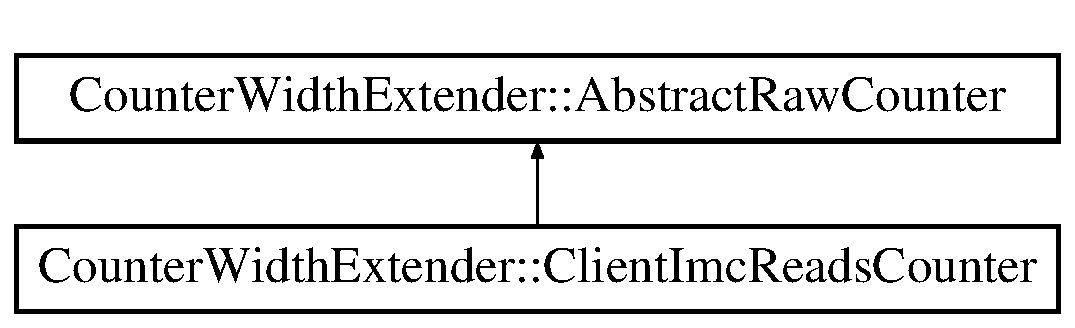
\includegraphics[height=2.000000cm]{struct_counter_width_extender_1_1_client_imc_reads_counter}
\end{center}
\end{figure}
\subsection*{Public Member Functions}
\begin{DoxyCompactItemize}
\item 
\mbox{\Hypertarget{struct_counter_width_extender_1_1_client_imc_reads_counter_abf1eb49eba1237aa421c17515d4f2cbc}\label{struct_counter_width_extender_1_1_client_imc_reads_counter_abf1eb49eba1237aa421c17515d4f2cbc}} 
{\bfseries Client\+Imc\+Reads\+Counter} (std\+::shared\+\_\+ptr$<$ \mbox{\hyperlink{class_client_b_w}{Client\+BW}} $>$ client\+B\+W\+\_\+)
\item 
\mbox{\Hypertarget{struct_counter_width_extender_1_1_client_imc_reads_counter_a2ce041afc601d13a4c19d75c2fae548f}\label{struct_counter_width_extender_1_1_client_imc_reads_counter_a2ce041afc601d13a4c19d75c2fae548f}} 
uint64 {\bfseries operator()} ()
\end{DoxyCompactItemize}
\subsection*{Public Attributes}
\begin{DoxyCompactItemize}
\item 
\mbox{\Hypertarget{struct_counter_width_extender_1_1_client_imc_reads_counter_a5bdef13d0d61c44507001729451d6222}\label{struct_counter_width_extender_1_1_client_imc_reads_counter_a5bdef13d0d61c44507001729451d6222}} 
std\+::shared\+\_\+ptr$<$ \mbox{\hyperlink{class_client_b_w}{Client\+BW}} $>$ {\bfseries client\+BW}
\end{DoxyCompactItemize}


The documentation for this struct was generated from the following file\+:\begin{DoxyCompactItemize}
\item 
\mbox{\hyperlink{width__extender_8h}{width\+\_\+extender.\+h}}\end{DoxyCompactItemize}

\hypertarget{struct_counter_width_extender_1_1_client_imc_writes_counter}{}\section{Counter\+Width\+Extender\+:\+:Client\+Imc\+Writes\+Counter Struct Reference}
\label{struct_counter_width_extender_1_1_client_imc_writes_counter}\index{Counter\+Width\+Extender\+::\+Client\+Imc\+Writes\+Counter@{Counter\+Width\+Extender\+::\+Client\+Imc\+Writes\+Counter}}
Inheritance diagram for Counter\+Width\+Extender\+:\+:Client\+Imc\+Writes\+Counter\+:\begin{figure}[H]
\begin{center}
\leavevmode
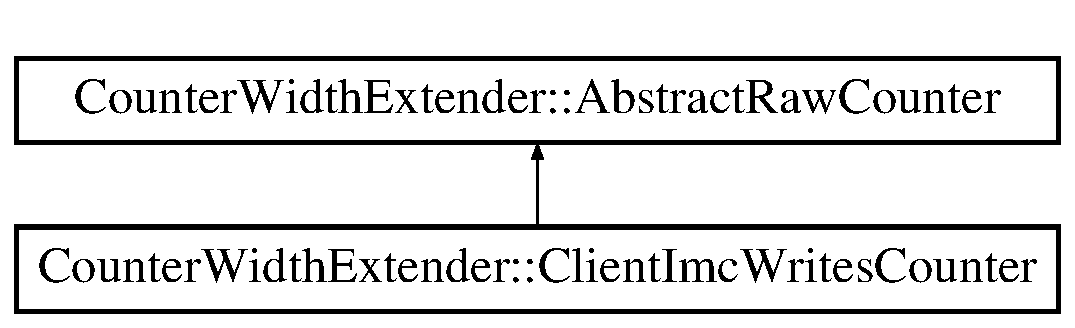
\includegraphics[height=2.000000cm]{struct_counter_width_extender_1_1_client_imc_writes_counter}
\end{center}
\end{figure}
\subsection*{Public Member Functions}
\begin{DoxyCompactItemize}
\item 
\mbox{\Hypertarget{struct_counter_width_extender_1_1_client_imc_writes_counter_a7df3cec47a653dadcb46368a5a3a1e85}\label{struct_counter_width_extender_1_1_client_imc_writes_counter_a7df3cec47a653dadcb46368a5a3a1e85}} 
{\bfseries Client\+Imc\+Writes\+Counter} (std\+::shared\+\_\+ptr$<$ \mbox{\hyperlink{class_client_b_w}{Client\+BW}} $>$ client\+B\+W\+\_\+)
\item 
\mbox{\Hypertarget{struct_counter_width_extender_1_1_client_imc_writes_counter_a3156907cb67016aea3255b75d7a887cb}\label{struct_counter_width_extender_1_1_client_imc_writes_counter_a3156907cb67016aea3255b75d7a887cb}} 
uint64 {\bfseries operator()} ()
\end{DoxyCompactItemize}
\subsection*{Public Attributes}
\begin{DoxyCompactItemize}
\item 
\mbox{\Hypertarget{struct_counter_width_extender_1_1_client_imc_writes_counter_a4dcb0451c4b5797040d3c439447312fc}\label{struct_counter_width_extender_1_1_client_imc_writes_counter_a4dcb0451c4b5797040d3c439447312fc}} 
std\+::shared\+\_\+ptr$<$ \mbox{\hyperlink{class_client_b_w}{Client\+BW}} $>$ {\bfseries client\+BW}
\end{DoxyCompactItemize}


The documentation for this struct was generated from the following file\+:\begin{DoxyCompactItemize}
\item 
\mbox{\hyperlink{width__extender_8h}{width\+\_\+extender.\+h}}\end{DoxyCompactItemize}

\hypertarget{struct_counter_width_extender_1_1_client_io_requests_counter}{}\section{Counter\+Width\+Extender\+:\+:Client\+Io\+Requests\+Counter Struct Reference}
\label{struct_counter_width_extender_1_1_client_io_requests_counter}\index{Counter\+Width\+Extender\+::\+Client\+Io\+Requests\+Counter@{Counter\+Width\+Extender\+::\+Client\+Io\+Requests\+Counter}}
Inheritance diagram for Counter\+Width\+Extender\+:\+:Client\+Io\+Requests\+Counter\+:\begin{figure}[H]
\begin{center}
\leavevmode
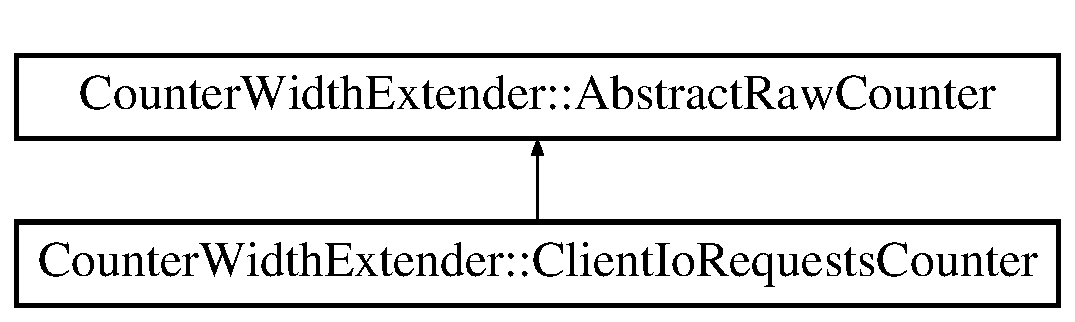
\includegraphics[height=2.000000cm]{struct_counter_width_extender_1_1_client_io_requests_counter}
\end{center}
\end{figure}
\subsection*{Public Member Functions}
\begin{DoxyCompactItemize}
\item 
\mbox{\Hypertarget{struct_counter_width_extender_1_1_client_io_requests_counter_ab3e30c3abdcbd4606e8bb86749abed85}\label{struct_counter_width_extender_1_1_client_io_requests_counter_ab3e30c3abdcbd4606e8bb86749abed85}} 
{\bfseries Client\+Io\+Requests\+Counter} (std\+::shared\+\_\+ptr$<$ \mbox{\hyperlink{class_client_b_w}{Client\+BW}} $>$ client\+B\+W\+\_\+)
\item 
\mbox{\Hypertarget{struct_counter_width_extender_1_1_client_io_requests_counter_a13cfbc3fedce8d039b306c303f485ff8}\label{struct_counter_width_extender_1_1_client_io_requests_counter_a13cfbc3fedce8d039b306c303f485ff8}} 
uint64 {\bfseries operator()} ()
\end{DoxyCompactItemize}
\subsection*{Public Attributes}
\begin{DoxyCompactItemize}
\item 
\mbox{\Hypertarget{struct_counter_width_extender_1_1_client_io_requests_counter_a00d1a9c0c690843010b82d59fe1ab0b2}\label{struct_counter_width_extender_1_1_client_io_requests_counter_a00d1a9c0c690843010b82d59fe1ab0b2}} 
std\+::shared\+\_\+ptr$<$ \mbox{\hyperlink{class_client_b_w}{Client\+BW}} $>$ {\bfseries client\+BW}
\end{DoxyCompactItemize}


The documentation for this struct was generated from the following file\+:\begin{DoxyCompactItemize}
\item 
\mbox{\hyperlink{width__extender_8h}{width\+\_\+extender.\+h}}\end{DoxyCompactItemize}

\hypertarget{class_core_counter_state}{}\section{Core\+Counter\+State Class Reference}
\label{class_core_counter_state}\index{Core\+Counter\+State@{Core\+Counter\+State}}


(Logical) core-\/wide counter state  




{\ttfamily \#include $<$cpucounters.\+h$>$}

Inheritance diagram for Core\+Counter\+State\+:\begin{figure}[H]
\begin{center}
\leavevmode
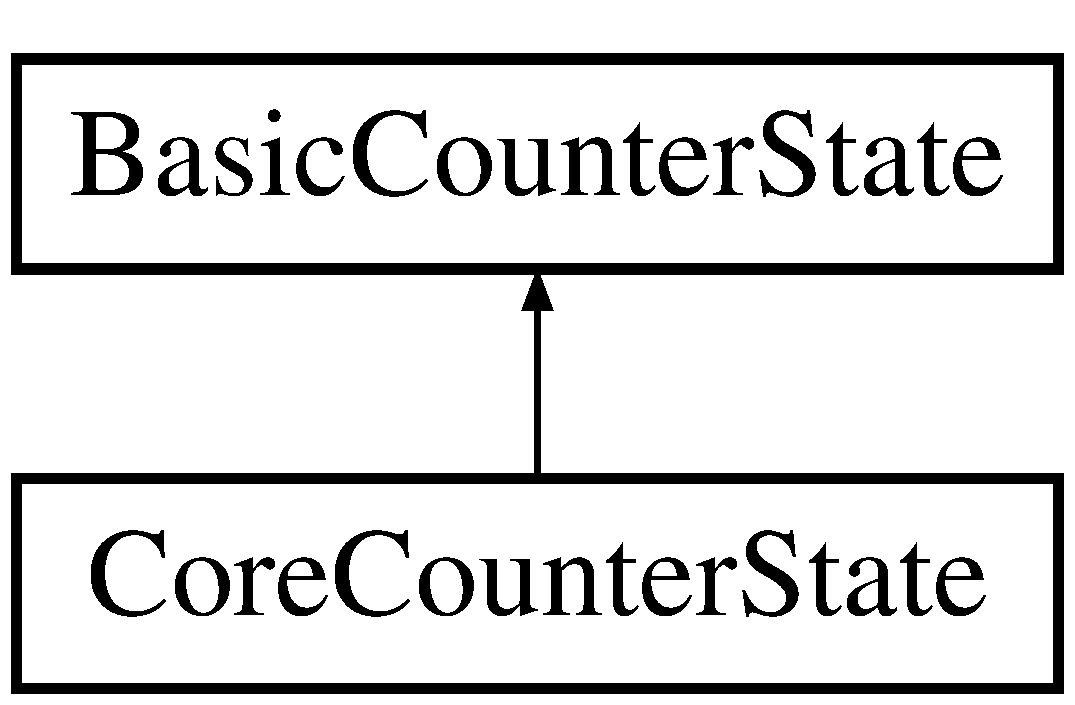
\includegraphics[height=2.000000cm]{class_core_counter_state}
\end{center}
\end{figure}
\subsection*{Friends}
\begin{DoxyCompactItemize}
\item 
\mbox{\Hypertarget{class_core_counter_state_ab5f56d2e95ba3daf52c17b8a1d356d64}\label{class_core_counter_state_ab5f56d2e95ba3daf52c17b8a1d356d64}} 
class {\bfseries P\+CM}
\end{DoxyCompactItemize}
\subsection*{Additional Inherited Members}


\subsection{Detailed Description}
(Logical) core-\/wide counter state 

The documentation for this class was generated from the following file\+:\begin{DoxyCompactItemize}
\item 
\mbox{\hyperlink{cpucounters_8h}{cpucounters.\+h}}\end{DoxyCompactItemize}

\hypertarget{struct_core_event}{}\section{Core\+Event Struct Reference}
\label{struct_core_event}\index{Core\+Event@{Core\+Event}}
\subsection*{Public Attributes}
\begin{DoxyCompactItemize}
\item 
\mbox{\Hypertarget{struct_core_event_adfc317377ca5e570e76cefb0bcb956a7}\label{struct_core_event_adfc317377ca5e570e76cefb0bcb956a7}} 
char {\bfseries name} \mbox{[}256\mbox{]}
\item 
\mbox{\Hypertarget{struct_core_event_aee18e455c55f0af436f9232e80eba77d}\label{struct_core_event_aee18e455c55f0af436f9232e80eba77d}} 
uint64 {\bfseries value}
\item 
\mbox{\Hypertarget{struct_core_event_a6bea66846abee2af316f5c38069d0768}\label{struct_core_event_a6bea66846abee2af316f5c38069d0768}} 
uint64 {\bfseries msr\+\_\+value}
\item 
\mbox{\Hypertarget{struct_core_event_a938a4c4c72139b70a6a647698e4a2121}\label{struct_core_event_a938a4c4c72139b70a6a647698e4a2121}} 
char $\ast$ {\bfseries description}
\end{DoxyCompactItemize}


The documentation for this struct was generated from the following file\+:\begin{DoxyCompactItemize}
\item 
\mbox{\hyperlink{pcm-core_8cpp}{pcm-\/core.\+cpp}}\end{DoxyCompactItemize}

\hypertarget{class_core_task_queue}{}\section{Core\+Task\+Queue Class Reference}
\label{class_core_task_queue}\index{Core\+Task\+Queue@{Core\+Task\+Queue}}
\subsection*{Public Member Functions}
\begin{DoxyCompactItemize}
\item 
\mbox{\Hypertarget{class_core_task_queue_ae0748611bfea1406cdcae5469e6983ec}\label{class_core_task_queue_ae0748611bfea1406cdcae5469e6983ec}} 
{\bfseries Core\+Task\+Queue} (int32 core)
\item 
\mbox{\Hypertarget{class_core_task_queue_affede6b8b5d78bbf64214f7a2f2badaf}\label{class_core_task_queue_affede6b8b5d78bbf64214f7a2f2badaf}} 
void {\bfseries push} (std\+::packaged\+\_\+task$<$ void()$>$ \&task)
\end{DoxyCompactItemize}


The documentation for this class was generated from the following file\+:\begin{DoxyCompactItemize}
\item 
\mbox{\hyperlink{cpucounters_8cpp}{cpucounters.\+cpp}}\end{DoxyCompactItemize}

\hypertarget{structcounter}{}\section{counter Struct Reference}
\label{structcounter}\index{counter@{counter}}
\subsection*{Public Attributes}
\begin{DoxyCompactItemize}
\item 
\mbox{\Hypertarget{structcounter_addb64347e960e0b7535b4992bec1f522}\label{structcounter_addb64347e960e0b7535b4992bec1f522}} 
string {\bfseries h\+\_\+event\+\_\+name}
\item 
\mbox{\Hypertarget{structcounter_add48f1203e73fd7c50564babbe8b6176}\label{structcounter_add48f1203e73fd7c50564babbe8b6176}} 
string {\bfseries v\+\_\+event\+\_\+name}
\item 
\mbox{\Hypertarget{structcounter_a63457f99b045b0811071b9584557238f}\label{structcounter_a63457f99b045b0811071b9584557238f}} 
\mbox{\hyperlink{struct_i_i_o_p_m_u_c_n_t_c_t_l_register}{I\+I\+O\+P\+M\+U\+C\+N\+T\+C\+T\+L\+Register}} {\bfseries Opcodes}
\item 
\mbox{\Hypertarget{structcounter_aa6611db7a280c8bb6bf4e19506bc6a02}\label{structcounter_aa6611db7a280c8bb6bf4e19506bc6a02}} 
int {\bfseries idx}
\item 
\mbox{\Hypertarget{structcounter_ac3b51026bf7769fe85471d2f7f914c49}\label{structcounter_ac3b51026bf7769fe85471d2f7f914c49}} 
int {\bfseries multiplier}
\item 
\mbox{\Hypertarget{structcounter_a97ec3319c8309f41de78490a46cb5e55}\label{structcounter_a97ec3319c8309f41de78490a46cb5e55}} 
int {\bfseries divider}
\item 
\mbox{\Hypertarget{structcounter_ac4cc48aebe0bd4cdc697b9023f41ab0e}\label{structcounter_ac4cc48aebe0bd4cdc697b9023f41ab0e}} 
uint32\+\_\+t {\bfseries h\+\_\+id}
\item 
\mbox{\Hypertarget{structcounter_a5c5c189e06e1164376c56b639b061f11}\label{structcounter_a5c5c189e06e1164376c56b639b061f11}} 
uint32\+\_\+t {\bfseries v\+\_\+id}
\item 
\mbox{\Hypertarget{structcounter_a39cdc8ce37a5cc283eab5a362adc7f46}\label{structcounter_a39cdc8ce37a5cc283eab5a362adc7f46}} 
vector$<$ result\+\_\+content $>$ {\bfseries data}
\end{DoxyCompactItemize}


The documentation for this struct was generated from the following file\+:\begin{DoxyCompactItemize}
\item 
lspci.\+h\end{DoxyCompactItemize}

\hypertarget{class_counter_width_extender}{}\section{Counter\+Width\+Extender Class Reference}
\label{class_counter_width_extender}\index{Counter\+Width\+Extender@{Counter\+Width\+Extender}}
\subsection*{Classes}
\begin{DoxyCompactItemize}
\item 
struct \mbox{\hyperlink{struct_counter_width_extender_1_1_abstract_raw_counter}{Abstract\+Raw\+Counter}}
\item 
struct \mbox{\hyperlink{struct_counter_width_extender_1_1_client_imc_reads_counter}{Client\+Imc\+Reads\+Counter}}
\item 
struct \mbox{\hyperlink{struct_counter_width_extender_1_1_client_imc_writes_counter}{Client\+Imc\+Writes\+Counter}}
\item 
struct \mbox{\hyperlink{struct_counter_width_extender_1_1_client_io_requests_counter}{Client\+Io\+Requests\+Counter}}
\item 
struct \mbox{\hyperlink{struct_counter_width_extender_1_1_m_b_l_counter}{M\+B\+L\+Counter}}
\item 
struct \mbox{\hyperlink{struct_counter_width_extender_1_1_m_b_t_counter}{M\+B\+T\+Counter}}
\item 
struct \mbox{\hyperlink{struct_counter_width_extender_1_1_msr_handle_counter}{Msr\+Handle\+Counter}}
\end{DoxyCompactItemize}
\subsection*{Public Member Functions}
\begin{DoxyCompactItemize}
\item 
\mbox{\Hypertarget{class_counter_width_extender_a3d82385d83e31ef043103407883ee0fd}\label{class_counter_width_extender_a3d82385d83e31ef043103407883ee0fd}} 
{\bfseries Counter\+Width\+Extender} (\mbox{\hyperlink{struct_counter_width_extender_1_1_abstract_raw_counter}{Abstract\+Raw\+Counter}} $\ast$raw\+\_\+counter\+\_\+, uint64 counter\+\_\+width\+\_\+, uint32 watchdog\+\_\+delay\+\_\+ms\+\_\+)
\item 
\mbox{\Hypertarget{class_counter_width_extender_a481ee1b6002b489711f7c8f2e17729f3}\label{class_counter_width_extender_a481ee1b6002b489711f7c8f2e17729f3}} 
uint64 {\bfseries read} ()
\item 
\mbox{\Hypertarget{class_counter_width_extender_a4b175035962a1f6b925077c3d3e02de1}\label{class_counter_width_extender_a4b175035962a1f6b925077c3d3e02de1}} 
void {\bfseries reset} ()
\end{DoxyCompactItemize}


The documentation for this class was generated from the following files\+:\begin{DoxyCompactItemize}
\item 
\mbox{\hyperlink{width__extender_8h}{width\+\_\+extender.\+h}}\item 
\mbox{\hyperlink{cpucounters_8cpp}{cpucounters.\+cpp}}\end{DoxyCompactItemize}

\hypertarget{struct_p_c_m_1_1_custom_core_event_description}{}\section{P\+CM\+:\+:Custom\+Core\+Event\+Description Struct Reference}
\label{struct_p_c_m_1_1_custom_core_event_description}\index{P\+C\+M\+::\+Custom\+Core\+Event\+Description@{P\+C\+M\+::\+Custom\+Core\+Event\+Description}}


Custom Core event description.  




{\ttfamily \#include $<$cpucounters.\+h$>$}

\subsection*{Public Attributes}
\begin{DoxyCompactItemize}
\item 
\mbox{\Hypertarget{struct_p_c_m_1_1_custom_core_event_description_adfdbff9cf7c5be78450884b7adbd48fb}\label{struct_p_c_m_1_1_custom_core_event_description_adfdbff9cf7c5be78450884b7adbd48fb}} 
int32 {\bfseries event\+\_\+number}
\item 
\mbox{\Hypertarget{struct_p_c_m_1_1_custom_core_event_description_a317a16603c27cf815fa62d88e7fd2f61}\label{struct_p_c_m_1_1_custom_core_event_description_a317a16603c27cf815fa62d88e7fd2f61}} 
int32 {\bfseries umask\+\_\+value}
\end{DoxyCompactItemize}


\subsection{Detailed Description}
Custom Core event description. 

See \char`\"{}\+Intel 64 and I\+A-\/32 Architectures Software Developers Manual Volume 3\+B\+:
\+System Programming Guide, Part 2\char`\"{} for the concrete values of the data structure fields, e.\+g. Appendix A.\+2 \char`\"{}\+Performance Monitoring Events for Intel(r) Core(tm) Processor Family
and Xeon Processor Family\char`\"{} 

The documentation for this struct was generated from the following file\+:\begin{DoxyCompactItemize}
\item 
\mbox{\hyperlink{cpucounters_8h}{cpucounters.\+h}}\end{DoxyCompactItemize}

\hypertarget{struct_p_c_m_1_1_custom_i_i_o_event_description}{}\section{P\+CM\+:\+:Custom\+I\+I\+O\+Event\+Description Struct Reference}
\label{struct_p_c_m_1_1_custom_i_i_o_event_description}\index{P\+C\+M\+::\+Custom\+I\+I\+O\+Event\+Description@{P\+C\+M\+::\+Custom\+I\+I\+O\+Event\+Description}}
\subsection*{Public Attributes}
\begin{DoxyCompactItemize}
\item 
\mbox{\Hypertarget{struct_p_c_m_1_1_custom_i_i_o_event_description_af615c81f40d39e8770822313cd5fdbb6}\label{struct_p_c_m_1_1_custom_i_i_o_event_description_af615c81f40d39e8770822313cd5fdbb6}} 
std\+::string {\bfseries event\+Names} \mbox{[}4\mbox{]}
\item 
\mbox{\Hypertarget{struct_p_c_m_1_1_custom_i_i_o_event_description_a6bb56f124b443dfb2a46b203488cb451}\label{struct_p_c_m_1_1_custom_i_i_o_event_description_a6bb56f124b443dfb2a46b203488cb451}} 
\mbox{\hyperlink{struct_i_i_o_p_m_u_c_n_t_c_t_l_register}{I\+I\+O\+P\+M\+U\+C\+N\+T\+C\+T\+L\+Register}} {\bfseries event\+Opcodes} \mbox{[}4\mbox{]}
\item 
\mbox{\Hypertarget{struct_p_c_m_1_1_custom_i_i_o_event_description_a7953c1b84fd3b592b1b703a646c48e21}\label{struct_p_c_m_1_1_custom_i_i_o_event_description_a7953c1b84fd3b592b1b703a646c48e21}} 
int {\bfseries multiplier} \mbox{[}4\mbox{]}
\item 
\mbox{\Hypertarget{struct_p_c_m_1_1_custom_i_i_o_event_description_ae143fcdb7aa0f4c1cf5fb7f0767754e3}\label{struct_p_c_m_1_1_custom_i_i_o_event_description_ae143fcdb7aa0f4c1cf5fb7f0767754e3}} 
int {\bfseries divider} \mbox{[}4\mbox{]}
\end{DoxyCompactItemize}


The documentation for this struct was generated from the following file\+:\begin{DoxyCompactItemize}
\item 
\mbox{\hyperlink{cpucounters_8h}{cpucounters.\+h}}\end{DoxyCompactItemize}

\hypertarget{structdata}{}\section{data Struct Reference}
\label{structdata}\index{data@{data}}
\subsection*{Public Attributes}
\begin{DoxyCompactItemize}
\item 
\mbox{\Hypertarget{structdata_a751af8cd5c196a997cf47c8e3c95802c}\label{structdata_a751af8cd5c196a997cf47c8e3c95802c}} 
uint32\+\_\+t {\bfseries width}
\item 
\mbox{\Hypertarget{structdata_aee26865f2660705b3461088f8946f54c}\label{structdata_aee26865f2660705b3461088f8946f54c}} 
uint64\+\_\+t {\bfseries value}
\end{DoxyCompactItemize}


The documentation for this struct was generated from the following file\+:\begin{DoxyCompactItemize}
\item 
pcm-\/iio.\+cpp\end{DoxyCompactItemize}

\hypertarget{struct_event_select_register}{}\section{Event\+Select\+Register Struct Reference}
\label{struct_event_select_register}\index{Event\+Select\+Register@{Event\+Select\+Register}}
\subsection*{Public Attributes}
\begin{DoxyCompactItemize}
\item 
\mbox{\Hypertarget{struct_event_select_register_a0d025caf9ccb643c4ba9c67e3d1a4bbf}\label{struct_event_select_register_a0d025caf9ccb643c4ba9c67e3d1a4bbf}} 
\begin{tabbing}
xx\=xx\=xx\=xx\=xx\=xx\=xx\=xx\=xx\=\kill
union \{\\
\>struct \{\\
\>\>uint64 {\bfseries event\_select}: 8\\
\>\>uint64 {\bfseries umask}: 8\\
\>\>uint64 {\bfseries usr}: 1\\
\>\>uint64 {\bfseries os}: 1\\
\>\>uint64 {\bfseries edge}: 1\\
\>\>uint64 {\bfseries pin\_control}: 1\\
\>\>uint64 {\bfseries apic\_int}: 1\\
\>\>uint64 {\bfseries any\_thread}: 1\\
\>\>uint64 {\bfseries enable}: 1\\
\>\>uint64 {\bfseries invert}: 1\\
\>\>uint64 {\bfseries cmask}: 8\\
\>\>uint64 {\bfseries in\_tx}: 1\\
\>\>uint64 {\bfseries in\_txcp}: 1\\
\>\>uint64 {\bfseries reservedX}: 30\\
\>\} {\bfseries fields}\\
\>uint64 {\bfseries value}\\
\}; \\

\end{tabbing}\end{DoxyCompactItemize}


The documentation for this struct was generated from the following file\+:\begin{DoxyCompactItemize}
\item 
\mbox{\hyperlink{types_8h}{types.\+h}}\end{DoxyCompactItemize}

\hypertarget{struct_p_c_m_1_1_extended_custom_core_event_description}{}\section{P\+CM\+:\+:Extended\+Custom\+Core\+Event\+Description Struct Reference}
\label{struct_p_c_m_1_1_extended_custom_core_event_description}\index{P\+C\+M\+::\+Extended\+Custom\+Core\+Event\+Description@{P\+C\+M\+::\+Extended\+Custom\+Core\+Event\+Description}}


Extended custom core event description.  




{\ttfamily \#include $<$cpucounters.\+h$>$}

\subsection*{Public Attributes}
\begin{DoxyCompactItemize}
\item 
\mbox{\Hypertarget{struct_p_c_m_1_1_extended_custom_core_event_description_a793e3dbd33a6bc37f800bb990777a543}\label{struct_p_c_m_1_1_extended_custom_core_event_description_a793e3dbd33a6bc37f800bb990777a543}} 
\mbox{\hyperlink{struct_fixed_event_control_register}{Fixed\+Event\+Control\+Register}} $\ast$ {\bfseries fixed\+Cfg}
\item 
\mbox{\Hypertarget{struct_p_c_m_1_1_extended_custom_core_event_description_ae66c1ea4e0b4ef493ee7d8c1f3245945}\label{struct_p_c_m_1_1_extended_custom_core_event_description_ae66c1ea4e0b4ef493ee7d8c1f3245945}} 
uint32 {\bfseries n\+G\+P\+Counters}
\item 
\mbox{\Hypertarget{struct_p_c_m_1_1_extended_custom_core_event_description_aa8f24e6871fe123345fd0141828374a1}\label{struct_p_c_m_1_1_extended_custom_core_event_description_aa8f24e6871fe123345fd0141828374a1}} 
\mbox{\hyperlink{struct_event_select_register}{Event\+Select\+Register}} $\ast$ {\bfseries gp\+Counter\+Cfg}
\item 
\mbox{\Hypertarget{struct_p_c_m_1_1_extended_custom_core_event_description_a2a1a8771723138bddbeae034c7710934}\label{struct_p_c_m_1_1_extended_custom_core_event_description_a2a1a8771723138bddbeae034c7710934}} 
uint64 {\bfseries Offcore\+Response\+Msr\+Value} \mbox{[}2\mbox{]}
\end{DoxyCompactItemize}


\subsection{Detailed Description}
Extended custom core event description. 

In contrast to \mbox{\hyperlink{struct_p_c_m_1_1_custom_core_event_description}{Custom\+Core\+Event\+Description}} supports configuration of all fields.

See \char`\"{}\+Intel 64 and I\+A-\/32 Architectures Software Developers Manual Volume 3\+B\+:
\+System Programming Guide, Part 2\char`\"{} for the concrete values of the data structure fields, e.\+g. Appendix A.\+2 \char`\"{}\+Performance Monitoring Events for Intel(r) Core(tm) Processor Family
and Xeon Processor Family\char`\"{} 

The documentation for this struct was generated from the following file\+:\begin{DoxyCompactItemize}
\item 
\mbox{\hyperlink{cpucounters_8h}{cpucounters.\+h}}\end{DoxyCompactItemize}

\hypertarget{struct_fixed_event_control_register}{}\section{Fixed\+Event\+Control\+Register Struct Reference}
\label{struct_fixed_event_control_register}\index{Fixed\+Event\+Control\+Register@{Fixed\+Event\+Control\+Register}}
\subsection*{Public Attributes}
\begin{DoxyCompactItemize}
\item 
\mbox{\Hypertarget{struct_fixed_event_control_register_a08d80e327beeeb53624e77d3f9101b68}\label{struct_fixed_event_control_register_a08d80e327beeeb53624e77d3f9101b68}} 
\begin{tabbing}
xx\=xx\=xx\=xx\=xx\=xx\=xx\=xx\=xx\=\kill
union \{\\
\>struct \{\\
\>\>uint64 {\bfseries os0}: 1\\
\>\>uint64 {\bfseries usr0}: 1\\
\>\>uint64 {\bfseries any\_thread0}: 1\\
\>\>uint64 {\bfseries enable\_pmi0}: 1\\
\>\>uint64 {\bfseries os1}: 1\\
\>\>uint64 {\bfseries usr1}: 1\\
\>\>uint64 {\bfseries any\_thread1}: 1\\
\>\>uint64 {\bfseries enable\_pmi1}: 1\\
\>\>uint64 {\bfseries os2}: 1\\
\>\>uint64 {\bfseries usr2}: 1\\
\>\>uint64 {\bfseries any\_thread2}: 1\\
\>\>uint64 {\bfseries enable\_pmi2}: 1\\
\>\>uint64 {\bfseries reserved1}: 52\\
\>\} {\bfseries fields}\\
\>uint64 {\bfseries value}\\
\}; \\

\end{tabbing}\end{DoxyCompactItemize}


The documentation for this struct was generated from the following file\+:\begin{DoxyCompactItemize}
\item 
\mbox{\hyperlink{types_8h}{types.\+h}}\end{DoxyCompactItemize}

\hypertarget{structiio__skx}{}\section{iio\+\_\+skx Struct Reference}
\label{structiio__skx}\index{iio\+\_\+skx@{iio\+\_\+skx}}
\subsection*{Public Attributes}
\begin{DoxyCompactItemize}
\item 
\mbox{\Hypertarget{structiio__skx_af65224d4b81ac82ae65de48cfa35b5cb}\label{structiio__skx_af65224d4b81ac82ae65de48cfa35b5cb}} 
\begin{tabbing}
xx\=xx\=xx\=xx\=xx\=xx\=xx\=xx\=xx\=\kill
struct \{\\
\>struct \{\\
\>\>struct \mbox{\hyperlink{structpci}{pci}} {\bfseries root\_pci\_dev}\\
\>\>vector$<$ struct \mbox{\hyperlink{structpci}{pci}} $>$ {\bfseries child\_pci\_devs}\\
\>\} {\bfseries parts} \mbox{[}4\mbox{]}\\
\>uint8\_t {\bfseries busno}\\
\>string {\bfseries stack\_name}\\
\>vector$<$ uint64\_t $>$ {\bfseries values}\\
\} {\bfseries stacks} \mbox{[}6\mbox{]}\\

\end{tabbing}\item 
\mbox{\Hypertarget{structiio__skx_ad384eb7a01209cddfffbdb7424740bd9}\label{structiio__skx_ad384eb7a01209cddfffbdb7424740bd9}} 
uint32\+\_\+t {\bfseries socket\+\_\+id}
\end{DoxyCompactItemize}


The documentation for this struct was generated from the following file\+:\begin{DoxyCompactItemize}
\item 
lspci.\+h\end{DoxyCompactItemize}

\hypertarget{struct_i_i_o_p_m_u_c_n_t_c_t_l_register}{}\section{I\+I\+O\+P\+M\+U\+C\+N\+T\+C\+T\+L\+Register Struct Reference}
\label{struct_i_i_o_p_m_u_c_n_t_c_t_l_register}\index{I\+I\+O\+P\+M\+U\+C\+N\+T\+C\+T\+L\+Register@{I\+I\+O\+P\+M\+U\+C\+N\+T\+C\+T\+L\+Register}}
\subsection*{Public Attributes}
\begin{DoxyCompactItemize}
\item 
\mbox{\Hypertarget{struct_i_i_o_p_m_u_c_n_t_c_t_l_register_a7e53e8eb9f81e19a742cd30a5b6bca7b}\label{struct_i_i_o_p_m_u_c_n_t_c_t_l_register_a7e53e8eb9f81e19a742cd30a5b6bca7b}} 
\begin{tabbing}
xx\=xx\=xx\=xx\=xx\=xx\=xx\=xx\=xx\=\kill
union \{\\
\>struct \{\\
\>\>uint64 {\bfseries event\_select}: 8\\
\>\>uint64 {\bfseries umask}: 8\\
\>\>uint64 {\bfseries reserved1}: 1\\
\>\>uint64 {\bfseries reset}: 1\\
\>\>uint64 {\bfseries edge\_det}: 1\\
\>\>uint64 {\bfseries ignored}: 1\\
\>\>uint64 {\bfseries overflow\_enable}: 1\\
\>\>uint64 {\bfseries reserved2}: 1\\
\>\>uint64 {\bfseries enable}: 1\\
\>\>uint64 {\bfseries invert}: 1\\
\>\>uint64 {\bfseries thresh}: 12\\
\>\>uint64 {\bfseries ch\_mask}: 8\\
\>\>uint64 {\bfseries fc\_mask}: 3\\
\>\>uint64 {\bfseries reservedX}: 17\\
\>\} {\bfseries fields}\\
\>uint64 {\bfseries value}\\
\}; \\

\end{tabbing}\end{DoxyCompactItemize}


The documentation for this struct was generated from the following file\+:\begin{DoxyCompactItemize}
\item 
\mbox{\hyperlink{types_8h}{types.\+h}}\end{DoxyCompactItemize}

\hypertarget{class_instance_lock}{}\section{Instance\+Lock Class Reference}
\label{class_instance_lock}\index{Instance\+Lock@{Instance\+Lock}}
\subsection*{Public Member Functions}
\begin{DoxyCompactItemize}
\item 
\mbox{\Hypertarget{class_instance_lock_a9fa936c0a79760e8fe4e93a7bee72cb1}\label{class_instance_lock_a9fa936c0a79760e8fe4e93a7bee72cb1}} 
{\bfseries Instance\+Lock} (const bool global\+\_\+)
\end{DoxyCompactItemize}


The documentation for this class was generated from the following file\+:\begin{DoxyCompactItemize}
\item 
\mbox{\hyperlink{cpucounters_8cpp}{cpucounters.\+cpp}}\end{DoxyCompactItemize}

\hypertarget{struct_counter_width_extender_1_1_m_b_l_counter}{}\section{Counter\+Width\+Extender\+:\+:M\+B\+L\+Counter Struct Reference}
\label{struct_counter_width_extender_1_1_m_b_l_counter}\index{Counter\+Width\+Extender\+::\+M\+B\+L\+Counter@{Counter\+Width\+Extender\+::\+M\+B\+L\+Counter}}
Inheritance diagram for Counter\+Width\+Extender\+:\+:M\+B\+L\+Counter\+:\begin{figure}[H]
\begin{center}
\leavevmode
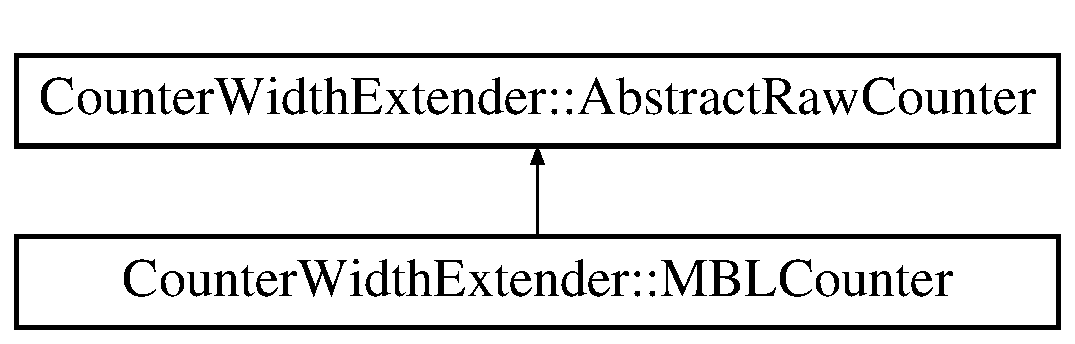
\includegraphics[height=2.000000cm]{struct_counter_width_extender_1_1_m_b_l_counter}
\end{center}
\end{figure}
\subsection*{Public Member Functions}
\begin{DoxyCompactItemize}
\item 
\mbox{\Hypertarget{struct_counter_width_extender_1_1_m_b_l_counter_ac13b8a75a9f0e948d105f4d4b0039c96}\label{struct_counter_width_extender_1_1_m_b_l_counter_ac13b8a75a9f0e948d105f4d4b0039c96}} 
{\bfseries M\+B\+L\+Counter} (std\+::shared\+\_\+ptr$<$ \mbox{\hyperlink{class_safe_msr_handle}{Safe\+Msr\+Handle}} $>$ msr\+\_\+)
\item 
\mbox{\Hypertarget{struct_counter_width_extender_1_1_m_b_l_counter_a59d60249fca8c0ebbfda0fb907a8541b}\label{struct_counter_width_extender_1_1_m_b_l_counter_a59d60249fca8c0ebbfda0fb907a8541b}} 
uint64 {\bfseries operator()} ()
\end{DoxyCompactItemize}
\subsection*{Public Attributes}
\begin{DoxyCompactItemize}
\item 
\mbox{\Hypertarget{struct_counter_width_extender_1_1_m_b_l_counter_a59be96131241a483193530c52258ad00}\label{struct_counter_width_extender_1_1_m_b_l_counter_a59be96131241a483193530c52258ad00}} 
std\+::shared\+\_\+ptr$<$ \mbox{\hyperlink{class_safe_msr_handle}{Safe\+Msr\+Handle}} $>$ {\bfseries msr}
\end{DoxyCompactItemize}


The documentation for this struct was generated from the following file\+:\begin{DoxyCompactItemize}
\item 
\mbox{\hyperlink{width__extender_8h}{width\+\_\+extender.\+h}}\end{DoxyCompactItemize}

\hypertarget{struct_counter_width_extender_1_1_m_b_t_counter}{}\section{Counter\+Width\+Extender\+:\+:M\+B\+T\+Counter Struct Reference}
\label{struct_counter_width_extender_1_1_m_b_t_counter}\index{Counter\+Width\+Extender\+::\+M\+B\+T\+Counter@{Counter\+Width\+Extender\+::\+M\+B\+T\+Counter}}
Inheritance diagram for Counter\+Width\+Extender\+:\+:M\+B\+T\+Counter\+:\begin{figure}[H]
\begin{center}
\leavevmode
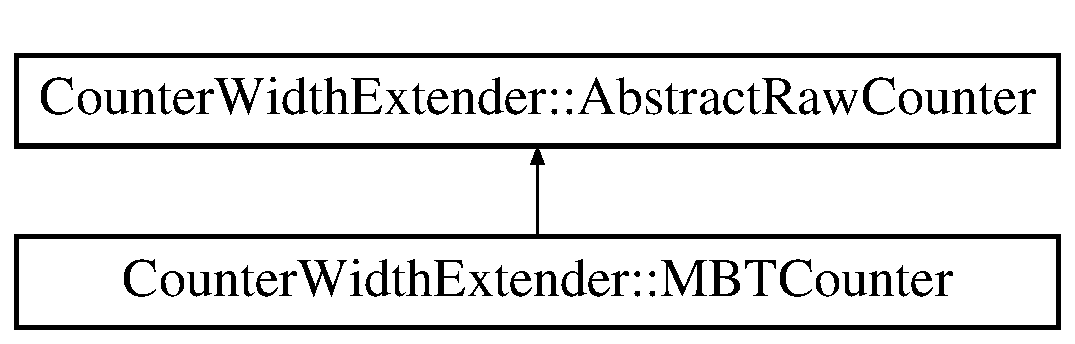
\includegraphics[height=2.000000cm]{struct_counter_width_extender_1_1_m_b_t_counter}
\end{center}
\end{figure}
\subsection*{Public Member Functions}
\begin{DoxyCompactItemize}
\item 
\mbox{\Hypertarget{struct_counter_width_extender_1_1_m_b_t_counter_a68bea99ee05808321fb3422831e816e4}\label{struct_counter_width_extender_1_1_m_b_t_counter_a68bea99ee05808321fb3422831e816e4}} 
{\bfseries M\+B\+T\+Counter} (std\+::shared\+\_\+ptr$<$ \mbox{\hyperlink{class_safe_msr_handle}{Safe\+Msr\+Handle}} $>$ msr\+\_\+)
\item 
\mbox{\Hypertarget{struct_counter_width_extender_1_1_m_b_t_counter_a0d2b7e5e23c4a0b02a00d27080a37ae3}\label{struct_counter_width_extender_1_1_m_b_t_counter_a0d2b7e5e23c4a0b02a00d27080a37ae3}} 
uint64 {\bfseries operator()} ()
\end{DoxyCompactItemize}
\subsection*{Public Attributes}
\begin{DoxyCompactItemize}
\item 
\mbox{\Hypertarget{struct_counter_width_extender_1_1_m_b_t_counter_acd71c78ec1b5fd68ccdc6cbdd3713342}\label{struct_counter_width_extender_1_1_m_b_t_counter_acd71c78ec1b5fd68ccdc6cbdd3713342}} 
std\+::shared\+\_\+ptr$<$ \mbox{\hyperlink{class_safe_msr_handle}{Safe\+Msr\+Handle}} $>$ {\bfseries msr}
\end{DoxyCompactItemize}


The documentation for this struct was generated from the following file\+:\begin{DoxyCompactItemize}
\item 
\mbox{\hyperlink{width__extender_8h}{width\+\_\+extender.\+h}}\end{DoxyCompactItemize}

\hypertarget{struct_m_c_f_g_header}{}\section{M\+C\+F\+G\+Header Struct Reference}
\label{struct_m_c_f_g_header}\index{M\+C\+F\+G\+Header@{M\+C\+F\+G\+Header}}
\subsection*{Public Member Functions}
\begin{DoxyCompactItemize}
\item 
\mbox{\Hypertarget{struct_m_c_f_g_header_ae69ced6c5f13fae4af9182ae37e333e7}\label{struct_m_c_f_g_header_ae69ced6c5f13fae4af9182ae37e333e7}} 
unsigned {\bfseries nrecords} () const
\item 
\mbox{\Hypertarget{struct_m_c_f_g_header_a3237441346fd64f80cb8b4b24aaa04cc}\label{struct_m_c_f_g_header_a3237441346fd64f80cb8b4b24aaa04cc}} 
void {\bfseries print} ()
\end{DoxyCompactItemize}
\subsection*{Public Attributes}
\begin{DoxyCompactItemize}
\item 
\mbox{\Hypertarget{struct_m_c_f_g_header_a22b92d6805395592f50b9e9bc29e10df}\label{struct_m_c_f_g_header_a22b92d6805395592f50b9e9bc29e10df}} 
char {\bfseries signature} \mbox{[}4\mbox{]}
\item 
\mbox{\Hypertarget{struct_m_c_f_g_header_a621db3813e8b6b1fa6a19c061efbfd02}\label{struct_m_c_f_g_header_a621db3813e8b6b1fa6a19c061efbfd02}} 
unsigned {\bfseries length}
\item 
\mbox{\Hypertarget{struct_m_c_f_g_header_a7f5a3f585900180ed744aa3a360beabf}\label{struct_m_c_f_g_header_a7f5a3f585900180ed744aa3a360beabf}} 
unsigned char {\bfseries revision}
\item 
\mbox{\Hypertarget{struct_m_c_f_g_header_ac4068aa15a9c7615a0b4b56c94317ad3}\label{struct_m_c_f_g_header_ac4068aa15a9c7615a0b4b56c94317ad3}} 
unsigned char {\bfseries checksum}
\item 
\mbox{\Hypertarget{struct_m_c_f_g_header_a41f92a0973011550d26aff4f3b127d97}\label{struct_m_c_f_g_header_a41f92a0973011550d26aff4f3b127d97}} 
char {\bfseries O\+E\+M\+ID} \mbox{[}6\mbox{]}
\item 
\mbox{\Hypertarget{struct_m_c_f_g_header_ad3d67bd8da58f78fb582561c9b5780ab}\label{struct_m_c_f_g_header_ad3d67bd8da58f78fb582561c9b5780ab}} 
char {\bfseries O\+E\+M\+Table\+ID} \mbox{[}8\mbox{]}
\item 
\mbox{\Hypertarget{struct_m_c_f_g_header_ab27a08c03ed5ec7a0c22681089269c9a}\label{struct_m_c_f_g_header_ab27a08c03ed5ec7a0c22681089269c9a}} 
unsigned {\bfseries O\+E\+M\+Revision}
\item 
\mbox{\Hypertarget{struct_m_c_f_g_header_af4ca343e759c3d8b1cc527d082d19ac0}\label{struct_m_c_f_g_header_af4ca343e759c3d8b1cc527d082d19ac0}} 
unsigned {\bfseries creator\+ID}
\item 
\mbox{\Hypertarget{struct_m_c_f_g_header_ada979c0affe38bf0c0c80f8de6356bb4}\label{struct_m_c_f_g_header_ada979c0affe38bf0c0c80f8de6356bb4}} 
unsigned {\bfseries creator\+Revision}
\item 
\mbox{\Hypertarget{struct_m_c_f_g_header_ab705b7e929202f5876da9e0a6d474c7b}\label{struct_m_c_f_g_header_ab705b7e929202f5876da9e0a6d474c7b}} 
char {\bfseries reserved} \mbox{[}8\mbox{]}
\end{DoxyCompactItemize}


The documentation for this struct was generated from the following file\+:\begin{DoxyCompactItemize}
\item 
\mbox{\hyperlink{types_8h}{types.\+h}}\end{DoxyCompactItemize}

\hypertarget{struct_m_c_f_g_record}{}\section{M\+C\+F\+G\+Record Struct Reference}
\label{struct_m_c_f_g_record}\index{M\+C\+F\+G\+Record@{M\+C\+F\+G\+Record}}
\subsection*{Public Member Functions}
\begin{DoxyCompactItemize}
\item 
\mbox{\Hypertarget{struct_m_c_f_g_record_a4b954297f9dd2db580af3305dc2c1200}\label{struct_m_c_f_g_record_a4b954297f9dd2db580af3305dc2c1200}} 
void {\bfseries print} ()
\end{DoxyCompactItemize}
\subsection*{Public Attributes}
\begin{DoxyCompactItemize}
\item 
\mbox{\Hypertarget{struct_m_c_f_g_record_ab80de5ed728d89f1bd60647e0e909289}\label{struct_m_c_f_g_record_ab80de5ed728d89f1bd60647e0e909289}} 
unsigned long long {\bfseries base\+Address}
\item 
\mbox{\Hypertarget{struct_m_c_f_g_record_a2ead77d33416e9f9a8607c7bdc9a3aa4}\label{struct_m_c_f_g_record_a2ead77d33416e9f9a8607c7bdc9a3aa4}} 
unsigned short {\bfseries P\+C\+I\+Segment\+Group\+Number}
\item 
\mbox{\Hypertarget{struct_m_c_f_g_record_a88a45ddf628776154cb5ed02b384061d}\label{struct_m_c_f_g_record_a88a45ddf628776154cb5ed02b384061d}} 
unsigned char {\bfseries start\+Bus\+Number}
\item 
\mbox{\Hypertarget{struct_m_c_f_g_record_a39692440cf50265f71b638d433a7ce37}\label{struct_m_c_f_g_record_a39692440cf50265f71b638d433a7ce37}} 
unsigned char {\bfseries end\+Bus\+Number}
\item 
\mbox{\Hypertarget{struct_m_c_f_g_record_a549591813ff09495f6ee59cb3288f130}\label{struct_m_c_f_g_record_a549591813ff09495f6ee59cb3288f130}} 
char {\bfseries reserved} \mbox{[}4\mbox{]}
\end{DoxyCompactItemize}


The documentation for this struct was generated from the following file\+:\begin{DoxyCompactItemize}
\item 
\mbox{\hyperlink{types_8h}{types.\+h}}\end{DoxyCompactItemize}

\hypertarget{structmemdata}{}\section{memdata Struct Reference}
\label{structmemdata}\index{memdata@{memdata}}
\subsection*{Public Attributes}
\begin{DoxyCompactItemize}
\item 
\mbox{\Hypertarget{structmemdata_ab6c2b2f802d5f0d69ddd546dcf21e142}\label{structmemdata_ab6c2b2f802d5f0d69ddd546dcf21e142}} 
float {\bfseries i\+M\+C\+\_\+\+Rd\+\_\+socket\+\_\+chan} \mbox{[}max\+\_\+sockets\mbox{]}\mbox{[}max\+\_\+imc\+\_\+channels\mbox{]}
\item 
\mbox{\Hypertarget{structmemdata_aeac15c4ce5b43f024cecca4c58f3b176}\label{structmemdata_aeac15c4ce5b43f024cecca4c58f3b176}} 
float {\bfseries i\+M\+C\+\_\+\+Wr\+\_\+socket\+\_\+chan} \mbox{[}max\+\_\+sockets\mbox{]}\mbox{[}max\+\_\+imc\+\_\+channels\mbox{]}
\item 
\mbox{\Hypertarget{structmemdata_aaf918650a303e6a99dc353263ade35a4}\label{structmemdata_aaf918650a303e6a99dc353263ade35a4}} 
float {\bfseries i\+M\+C\+\_\+\+Rd\+\_\+socket} \mbox{[}max\+\_\+sockets\mbox{]}
\item 
\mbox{\Hypertarget{structmemdata_a689eb20051fcd7d835ee5e685db6390f}\label{structmemdata_a689eb20051fcd7d835ee5e685db6390f}} 
float {\bfseries i\+M\+C\+\_\+\+Wr\+\_\+socket} \mbox{[}max\+\_\+sockets\mbox{]}
\item 
\mbox{\Hypertarget{structmemdata_a6b56866bb465b62662bf4fa7c1aced10}\label{structmemdata_a6b56866bb465b62662bf4fa7c1aced10}} 
float {\bfseries E\+D\+C\+\_\+\+Rd\+\_\+socket\+\_\+chan} \mbox{[}max\+\_\+sockets\mbox{]}\mbox{[}max\+\_\+edc\+\_\+channels\mbox{]}
\item 
\mbox{\Hypertarget{structmemdata_a4ca2b57f962b2d0d3649868a1a4199ba}\label{structmemdata_a4ca2b57f962b2d0d3649868a1a4199ba}} 
float {\bfseries E\+D\+C\+\_\+\+Wr\+\_\+socket\+\_\+chan} \mbox{[}max\+\_\+sockets\mbox{]}\mbox{[}max\+\_\+edc\+\_\+channels\mbox{]}
\item 
\mbox{\Hypertarget{structmemdata_a43eee155761fbebb23ce86a7ab954fff}\label{structmemdata_a43eee155761fbebb23ce86a7ab954fff}} 
float {\bfseries E\+D\+C\+\_\+\+Rd\+\_\+socket} \mbox{[}max\+\_\+sockets\mbox{]}
\item 
\mbox{\Hypertarget{structmemdata_afe5a628e9ad97b72fd12e7b6de78e784}\label{structmemdata_afe5a628e9ad97b72fd12e7b6de78e784}} 
float {\bfseries E\+D\+C\+\_\+\+Wr\+\_\+socket} \mbox{[}max\+\_\+sockets\mbox{]}
\item 
\mbox{\Hypertarget{structmemdata_a28e131c751efa29fd9b0670dcbb8e073}\label{structmemdata_a28e131c751efa29fd9b0670dcbb8e073}} 
uint64 {\bfseries partial\+\_\+write} \mbox{[}max\+\_\+sockets\mbox{]}
\end{DoxyCompactItemize}


The documentation for this struct was generated from the following file\+:\begin{DoxyCompactItemize}
\item 
\mbox{\hyperlink{pcm-memory_8cpp}{pcm-\/memory.\+cpp}}\end{DoxyCompactItemize}

\hypertarget{class_msr_handle}{}\section{Msr\+Handle Class Reference}
\label{class_msr_handle}\index{Msr\+Handle@{Msr\+Handle}}
\subsection*{Public Member Functions}
\begin{DoxyCompactItemize}
\item 
\mbox{\Hypertarget{class_msr_handle_a481b0c81ad8f00d9d69db660e793a135}\label{class_msr_handle_a481b0c81ad8f00d9d69db660e793a135}} 
{\bfseries Msr\+Handle} (uint32 cpu)
\item 
\mbox{\Hypertarget{class_msr_handle_a9a7723baaa1ec91a8303b5ef6579c1df}\label{class_msr_handle_a9a7723baaa1ec91a8303b5ef6579c1df}} 
int32 {\bfseries read} (uint64 msr\+\_\+number, uint64 $\ast$value)
\item 
\mbox{\Hypertarget{class_msr_handle_aa92da3c093ca1473eb7a7cad86f24c89}\label{class_msr_handle_aa92da3c093ca1473eb7a7cad86f24c89}} 
int32 {\bfseries write} (uint64 msr\+\_\+number, uint64 value)
\item 
\mbox{\Hypertarget{class_msr_handle_adbbfac37adfdd3fb571b5a6978f60419}\label{class_msr_handle_adbbfac37adfdd3fb571b5a6978f60419}} 
int32 {\bfseries get\+Core\+Id} ()
\end{DoxyCompactItemize}


The documentation for this class was generated from the following files\+:\begin{DoxyCompactItemize}
\item 
\mbox{\hyperlink{msr_8h}{msr.\+h}}\item 
msr.\+cpp\end{DoxyCompactItemize}

\hypertarget{struct_counter_width_extender_1_1_msr_handle_counter}{}\section{Counter\+Width\+Extender\+:\+:Msr\+Handle\+Counter Struct Reference}
\label{struct_counter_width_extender_1_1_msr_handle_counter}\index{Counter\+Width\+Extender\+::\+Msr\+Handle\+Counter@{Counter\+Width\+Extender\+::\+Msr\+Handle\+Counter}}
Inheritance diagram for Counter\+Width\+Extender\+:\+:Msr\+Handle\+Counter\+:\begin{figure}[H]
\begin{center}
\leavevmode
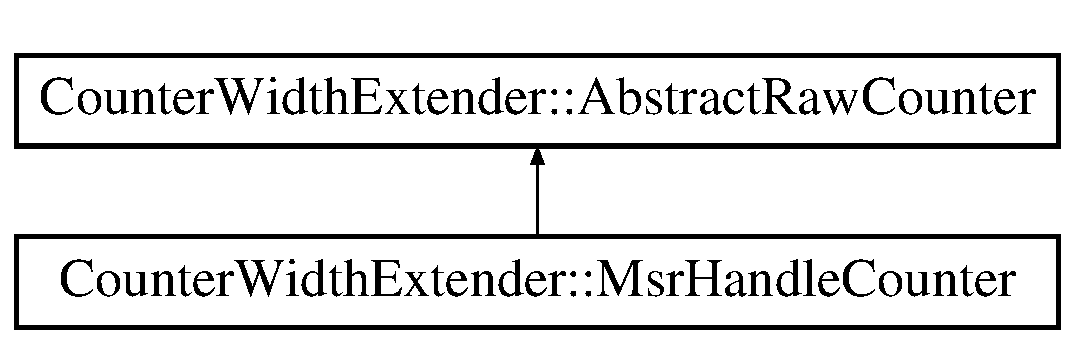
\includegraphics[height=2.000000cm]{struct_counter_width_extender_1_1_msr_handle_counter}
\end{center}
\end{figure}
\subsection*{Public Member Functions}
\begin{DoxyCompactItemize}
\item 
\mbox{\Hypertarget{struct_counter_width_extender_1_1_msr_handle_counter_a293eeb777712b8dff89999db5d671bc9}\label{struct_counter_width_extender_1_1_msr_handle_counter_a293eeb777712b8dff89999db5d671bc9}} 
{\bfseries Msr\+Handle\+Counter} (std\+::shared\+\_\+ptr$<$ \mbox{\hyperlink{class_safe_msr_handle}{Safe\+Msr\+Handle}} $>$ msr\+\_\+, uint64 msr\+\_\+addr\+\_\+)
\item 
\mbox{\Hypertarget{struct_counter_width_extender_1_1_msr_handle_counter_af6a1d4c47ab99efc52e87805b20457fc}\label{struct_counter_width_extender_1_1_msr_handle_counter_af6a1d4c47ab99efc52e87805b20457fc}} 
uint64 {\bfseries operator()} ()
\end{DoxyCompactItemize}
\subsection*{Public Attributes}
\begin{DoxyCompactItemize}
\item 
\mbox{\Hypertarget{struct_counter_width_extender_1_1_msr_handle_counter_a221afc246d9a2b0d9e902650fe28b9a1}\label{struct_counter_width_extender_1_1_msr_handle_counter_a221afc246d9a2b0d9e902650fe28b9a1}} 
std\+::shared\+\_\+ptr$<$ \mbox{\hyperlink{class_safe_msr_handle}{Safe\+Msr\+Handle}} $>$ {\bfseries msr}
\item 
\mbox{\Hypertarget{struct_counter_width_extender_1_1_msr_handle_counter_a5522d6a788192c2cb69b8d0c4fc0a9a1}\label{struct_counter_width_extender_1_1_msr_handle_counter_a5522d6a788192c2cb69b8d0c4fc0a9a1}} 
uint64 {\bfseries msr\+\_\+addr}
\end{DoxyCompactItemize}


The documentation for this struct was generated from the following file\+:\begin{DoxyCompactItemize}
\item 
\mbox{\hyperlink{width__extender_8h}{width\+\_\+extender.\+h}}\end{DoxyCompactItemize}

\hypertarget{class_p_c_m___util_1_1_mutex}{}\section{P\+C\+M\+\_\+\+Util\+:\+:Mutex Class Reference}
\label{class_p_c_m___util_1_1_mutex}\index{P\+C\+M\+\_\+\+Util\+::\+Mutex@{P\+C\+M\+\_\+\+Util\+::\+Mutex}}
\subsection*{Classes}
\begin{DoxyCompactItemize}
\item 
class \mbox{\hyperlink{class_p_c_m___util_1_1_mutex_1_1_scope}{Scope}}
\end{DoxyCompactItemize}
\subsection*{Public Member Functions}
\begin{DoxyCompactItemize}
\item 
\mbox{\Hypertarget{class_p_c_m___util_1_1_mutex_a04424b15dade04beb61030d077e20bc5}\label{class_p_c_m___util_1_1_mutex_a04424b15dade04beb61030d077e20bc5}} 
void {\bfseries lock} ()
\item 
\mbox{\Hypertarget{class_p_c_m___util_1_1_mutex_a0ed943ad319ecdbac0a8bb0072c0fdfb}\label{class_p_c_m___util_1_1_mutex_a0ed943ad319ecdbac0a8bb0072c0fdfb}} 
void {\bfseries unlock} ()
\end{DoxyCompactItemize}


The documentation for this class was generated from the following file\+:\begin{DoxyCompactItemize}
\item 
mutex.\+h\end{DoxyCompactItemize}

\hypertarget{structnull__stream}{}\section{null\+\_\+stream Struct Reference}
\label{structnull__stream}\index{null\+\_\+stream@{null\+\_\+stream}}
Inheritance diagram for null\+\_\+stream\+:\begin{figure}[H]
\begin{center}
\leavevmode
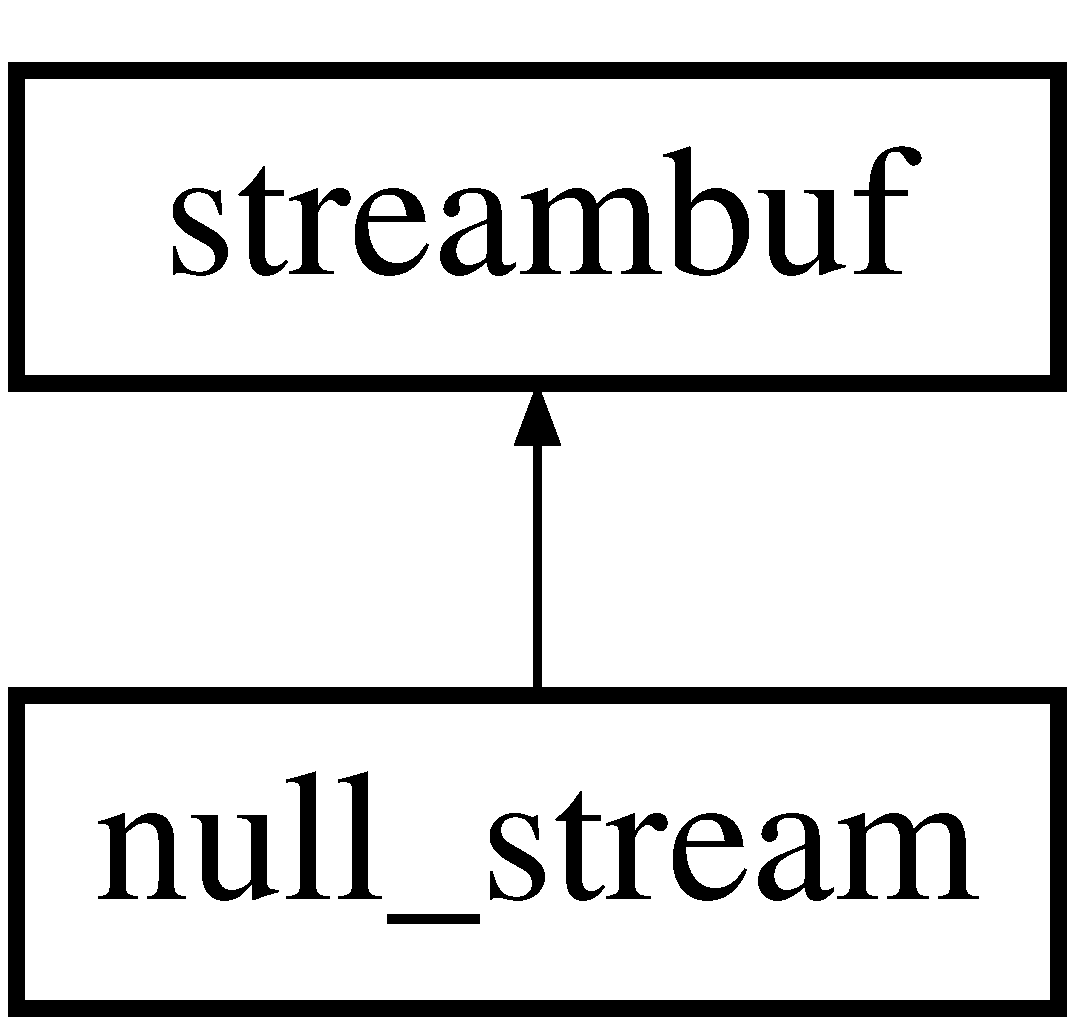
\includegraphics[height=2.000000cm]{structnull__stream}
\end{center}
\end{figure}
\subsection*{Public Member Functions}
\begin{DoxyCompactItemize}
\item 
\mbox{\Hypertarget{structnull__stream_a0bbaf9ee51c3dbe2583d3f2c0dfaeefb}\label{structnull__stream_a0bbaf9ee51c3dbe2583d3f2c0dfaeefb}} 
void {\bfseries overflow} (char)
\end{DoxyCompactItemize}


The documentation for this struct was generated from the following file\+:\begin{DoxyCompactItemize}
\item 
\mbox{\hyperlink{utils_8h}{utils.\+h}}\end{DoxyCompactItemize}

\hypertarget{structpci}{}\section{pci Struct Reference}
\label{structpci}\index{pci@{pci}}
\subsection*{Public Attributes}
\begin{DoxyCompactItemize}
\item 
\mbox{\Hypertarget{structpci_a4fbf5aef85cf6f114ef2c251d1d6c589}\label{structpci_a4fbf5aef85cf6f114ef2c251d1d6c589}} 
bool {\bfseries exist} = false
\item 
\mbox{\Hypertarget{structpci_a7a1fb1574c140948cd9f7fae2f621e0b}\label{structpci_a7a1fb1574c140948cd9f7fae2f621e0b}} 
struct \mbox{\hyperlink{structbdf}{bdf}} {\bfseries bdf}
\item 
\mbox{\Hypertarget{structpci_af70b39686d691ac28718d77909edd189}\label{structpci_af70b39686d691ac28718d77909edd189}} 
\begin{tabbing}
xx\=xx\=xx\=xx\=xx\=xx\=xx\=xx\=xx\=\kill
union \{\\
\mbox{\Hypertarget{unionpci_1_1_0D11_affa4816d356736545f3d9d51fafee616}\label{unionpci_1_1_0D11_affa4816d356736545f3d9d51fafee616}} 
\>struct \{\\
\>\>uint16\_t {\bfseries vendor\_id}\\
\>\>uint16\_t {\bfseries device\_id}\\
\>\} \\
\>uint32\_t {\bfseries offset\_0}\\
\}; \\

\end{tabbing}\item 
\mbox{\Hypertarget{structpci_a12b405a6b3ed7846f1e45cd06709e794}\label{structpci_a12b405a6b3ed7846f1e45cd06709e794}} 
int8\+\_\+t {\bfseries header\+\_\+type}
\item 
\mbox{\Hypertarget{structpci_a2834e29859bf5fbad19d4a23c5aa51d8}\label{structpci_a2834e29859bf5fbad19d4a23c5aa51d8}} 
\begin{tabbing}
xx\=xx\=xx\=xx\=xx\=xx\=xx\=xx\=xx\=\kill
union \{\\
\mbox{\Hypertarget{unionpci_1_1_0D13_a82f419dcc1fe1810804349324fab05ba}\label{unionpci_1_1_0D13_a82f419dcc1fe1810804349324fab05ba}} 
\>struct \{\\
\>\>uint8\_t {\bfseries primary\_bus\_number}\\
\>\>uint8\_t {\bfseries secondary\_bus\_number}\\
\>\>uint8\_t {\bfseries subordinate\_bus\_number}\\
\>\>uint8\_t {\bfseries junk}\\
\>\} \\
\>uint32\_t {\bfseries offset\_18}\\
\}; \\

\end{tabbing}\item 
\mbox{\Hypertarget{structpci_a50137b346b342d2ce39a58d0273ab6cd}\label{structpci_a50137b346b342d2ce39a58d0273ab6cd}} 
\begin{tabbing}
xx\=xx\=xx\=xx\=xx\=xx\=xx\=xx\=xx\=\kill
union \{\\
\mbox{\Hypertarget{unionpci_1_1_0D15_a981d2ed9425eaf4db7fec65fbd0e979e}\label{unionpci_1_1_0D15_a981d2ed9425eaf4db7fec65fbd0e979e}} 
\>struct \{\\
\>\>uint16\_t {\bfseries link\_ctrl}\\
\mbox{\Hypertarget{structpci_1_1_0D15_1_1_0D21_ac356c1dcee4a11e8bbe2b6c28c74aab8}\label{structpci_1_1_0D15_1_1_0D21_ac356c1dcee4a11e8bbe2b6c28c74aab8}} 
\>\>union \{\\
\mbox{\Hypertarget{unionpci_1_1_0D15_1_1_0D21_1_1_0D23_a1ae869adfe82220f16d40c4c49673b9e}\label{unionpci_1_1_0D15_1_1_0D21_1_1_0D23_a1ae869adfe82220f16d40c4c49673b9e}} 
\>\>\>struct \{\\
\>\>\>\>uint16\_t {\bfseries link\_speed}: 4\\
\>\>\>\>uint16\_t {\bfseries link\_width}: 6\\
\>\>\>\>uint16\_t {\bfseries undefined}: 1\\
\>\>\>\>uint16\_t {\bfseries link\_trained}: 1\\
\>\>\>\} \\
\>\>\>uint16\_t {\bfseries link\_sta}\\
\>\>\} \\
\>\} \\
\>uint32\_t {\bfseries link\_info}\\
\}; \\

\end{tabbing}\end{DoxyCompactItemize}


The documentation for this struct was generated from the following file\+:\begin{DoxyCompactItemize}
\item 
lspci.\+h\end{DoxyCompactItemize}

\hypertarget{struct_p_c_ie_events__t}{}\section{P\+C\+Ie\+Events\+\_\+t Struct Reference}
\label{struct_p_c_ie_events__t}\index{P\+C\+Ie\+Events\+\_\+t@{P\+C\+Ie\+Events\+\_\+t}}
\subsection*{Public Attributes}
\begin{DoxyCompactItemize}
\item 
\mbox{\Hypertarget{struct_p_c_ie_events__t_a433814915b2f0fb5673db7d42b5c8f01}\label{struct_p_c_ie_events__t_a433814915b2f0fb5673db7d42b5c8f01}} 
uint64 {\bfseries P\+C\+Ie\+Rd\+Cur}
\item 
\mbox{\Hypertarget{struct_p_c_ie_events__t_a72c70536a99db58c0ffbee2b0f949cb9}\label{struct_p_c_ie_events__t_a72c70536a99db58c0ffbee2b0f949cb9}} 
uint64 {\bfseries P\+C\+Ie\+N\+S\+Rd}
\item 
\mbox{\Hypertarget{struct_p_c_ie_events__t_a11255eae6dfabbe8f64f7b5ea818cd8a}\label{struct_p_c_ie_events__t_a11255eae6dfabbe8f64f7b5ea818cd8a}} 
uint64 {\bfseries P\+C\+Ie\+Wi\+LF}
\item 
\mbox{\Hypertarget{struct_p_c_ie_events__t_a6361b1a7d4ef44d4a9ce98be95ef1f98}\label{struct_p_c_ie_events__t_a6361b1a7d4ef44d4a9ce98be95ef1f98}} 
uint64 {\bfseries P\+C\+Ie\+ItoM}
\item 
\mbox{\Hypertarget{struct_p_c_ie_events__t_adc09e10dc946626835a246c2ad23f673}\label{struct_p_c_ie_events__t_adc09e10dc946626835a246c2ad23f673}} 
uint64 {\bfseries P\+C\+Ie\+N\+S\+Wr}
\item 
\mbox{\Hypertarget{struct_p_c_ie_events__t_afd92992ddfa7437bc37846ce8b26298b}\label{struct_p_c_ie_events__t_afd92992ddfa7437bc37846ce8b26298b}} 
uint64 {\bfseries P\+C\+Ie\+N\+S\+WrF}
\item 
\mbox{\Hypertarget{struct_p_c_ie_events__t_a22e3b41c0ce557fdbb8ff95b467ffbeb}\label{struct_p_c_ie_events__t_a22e3b41c0ce557fdbb8ff95b467ffbeb}} 
uint64 {\bfseries R\+FO}
\item 
\mbox{\Hypertarget{struct_p_c_ie_events__t_a6eb5d5b01e893a54069d20a1e8ab1e00}\label{struct_p_c_ie_events__t_a6eb5d5b01e893a54069d20a1e8ab1e00}} 
uint64 {\bfseries C\+Rd}
\item 
\mbox{\Hypertarget{struct_p_c_ie_events__t_aacf52abcf1e3417903975e9287b3ab8d}\label{struct_p_c_ie_events__t_aacf52abcf1e3417903975e9287b3ab8d}} 
uint64 {\bfseries D\+Rd}
\item 
\mbox{\Hypertarget{struct_p_c_ie_events__t_af24f33e0b4ed7b25606d5ef495b70c37}\label{struct_p_c_ie_events__t_af24f33e0b4ed7b25606d5ef495b70c37}} 
uint64 {\bfseries P\+Rd}
\item 
\mbox{\Hypertarget{struct_p_c_ie_events__t_a34ae70c8bf61d8a8d50fd671a3fb62b8}\label{struct_p_c_ie_events__t_a34ae70c8bf61d8a8d50fd671a3fb62b8}} 
uint64 {\bfseries WiL}
\item 
\mbox{\Hypertarget{struct_p_c_ie_events__t_a09e7e597f7eb1b569e6aefbe02dbf790}\label{struct_p_c_ie_events__t_a09e7e597f7eb1b569e6aefbe02dbf790}} 
uint64 {\bfseries ItoM}
\end{DoxyCompactItemize}


The documentation for this struct was generated from the following file\+:\begin{DoxyCompactItemize}
\item 
\mbox{\hyperlink{pcm-pcie_8cpp}{pcm-\/pcie.\+cpp}}\end{DoxyCompactItemize}

\hypertarget{class_pci_handle}{}\section{Pci\+Handle Class Reference}
\label{class_pci_handle}\index{Pci\+Handle@{Pci\+Handle}}
\subsection*{Public Member Functions}
\begin{DoxyCompactItemize}
\item 
\mbox{\Hypertarget{class_pci_handle_a95e2bf928bd4438831c5a3b5b516efe6}\label{class_pci_handle_a95e2bf928bd4438831c5a3b5b516efe6}} 
{\bfseries Pci\+Handle} (uint32 groupnr\+\_\+, uint32 bus\+\_\+, uint32 device\+\_\+, uint32 function\+\_\+)
\item 
\mbox{\Hypertarget{class_pci_handle_a76d15c7331d5fddd98d42e8a2316fb7c}\label{class_pci_handle_a76d15c7331d5fddd98d42e8a2316fb7c}} 
int32 {\bfseries read32} (uint64 offset, uint32 $\ast$value)
\item 
\mbox{\Hypertarget{class_pci_handle_a1975782af9943f65ba1312ff56fb30b1}\label{class_pci_handle_a1975782af9943f65ba1312ff56fb30b1}} 
int32 {\bfseries write32} (uint64 offset, uint32 value)
\item 
\mbox{\Hypertarget{class_pci_handle_a2f965ad969df3add9c955eaaeb43e715}\label{class_pci_handle_a2f965ad969df3add9c955eaaeb43e715}} 
int32 {\bfseries read64} (uint64 offset, uint64 $\ast$value)
\end{DoxyCompactItemize}
\subsection*{Static Public Member Functions}
\begin{DoxyCompactItemize}
\item 
\mbox{\Hypertarget{class_pci_handle_ac7eb1a7d50b8e345f75bdc8205592a92}\label{class_pci_handle_ac7eb1a7d50b8e345f75bdc8205592a92}} 
static bool {\bfseries exists} (uint32 groupnr\+\_\+, uint32 bus\+\_\+, uint32 device\+\_\+, uint32 function\+\_\+)
\end{DoxyCompactItemize}
\subsection*{Static Protected Member Functions}
\begin{DoxyCompactItemize}
\item 
static int \mbox{\hyperlink{class_pci_handle_a9b5105f02947177df61ffe78ee81f022}{open\+Mcfg\+Table}} ()
\end{DoxyCompactItemize}
\subsection*{Friends}
\begin{DoxyCompactItemize}
\item 
\mbox{\Hypertarget{class_pci_handle_ab4094f771b56aa375bccb1397e1a18bc}\label{class_pci_handle_ab4094f771b56aa375bccb1397e1a18bc}} 
class {\bfseries Pci\+HandleM}
\item 
\mbox{\Hypertarget{class_pci_handle_ad697cfb775e6784b97bf84b9f2a3938a}\label{class_pci_handle_ad697cfb775e6784b97bf84b9f2a3938a}} 
class {\bfseries Pci\+Handle\+MM}
\end{DoxyCompactItemize}


\subsection{Member Function Documentation}
\mbox{\Hypertarget{class_pci_handle_a9b5105f02947177df61ffe78ee81f022}\label{class_pci_handle_a9b5105f02947177df61ffe78ee81f022}} 
\index{Pci\+Handle@{Pci\+Handle}!open\+Mcfg\+Table@{open\+Mcfg\+Table}}
\index{open\+Mcfg\+Table@{open\+Mcfg\+Table}!Pci\+Handle@{Pci\+Handle}}
\subsubsection{\texorpdfstring{open\+Mcfg\+Table()}{openMcfgTable()}}
{\footnotesize\ttfamily int Pci\+Handle\+::open\+Mcfg\+Table (\begin{DoxyParamCaption}{ }\end{DoxyParamCaption})\hspace{0.3cm}{\ttfamily [static]}, {\ttfamily [protected]}}

There are no M\+C\+FG table on some machines, but M\+C\+F\+G1. See \href{https://github.com/opcm/pcm/issues/74}{\tt https\+://github.\+com/opcm/pcm/issues/74} for details

The documentation for this class was generated from the following files\+:\begin{DoxyCompactItemize}
\item 
\mbox{\hyperlink{pci_8h}{pci.\+h}}\item 
pci.\+cpp\end{DoxyCompactItemize}

\hypertarget{class_pci_handle_m}{}\section{Pci\+HandleM Class Reference}
\label{class_pci_handle_m}\index{Pci\+HandleM@{Pci\+HandleM}}
\subsection*{Public Member Functions}
\begin{DoxyCompactItemize}
\item 
\mbox{\Hypertarget{class_pci_handle_m_ad067fc750d7b2f05b9e67badbdf237d3}\label{class_pci_handle_m_ad067fc750d7b2f05b9e67badbdf237d3}} 
{\bfseries Pci\+HandleM} (uint32 bus\+\_\+, uint32 device\+\_\+, uint32 function\+\_\+)
\item 
\mbox{\Hypertarget{class_pci_handle_m_ac9257ce7ae864201459f4db8996de7f6}\label{class_pci_handle_m_ac9257ce7ae864201459f4db8996de7f6}} 
int32 {\bfseries read32} (uint64 offset, uint32 $\ast$value)
\item 
\mbox{\Hypertarget{class_pci_handle_m_a412df968cfe50c405aa445c2b52bf6b1}\label{class_pci_handle_m_a412df968cfe50c405aa445c2b52bf6b1}} 
int32 {\bfseries write32} (uint64 offset, uint32 value)
\item 
\mbox{\Hypertarget{class_pci_handle_m_a8fced207ab30a888b09ce361d1a45980}\label{class_pci_handle_m_a8fced207ab30a888b09ce361d1a45980}} 
int32 {\bfseries read64} (uint64 offset, uint64 $\ast$value)
\end{DoxyCompactItemize}
\subsection*{Static Public Member Functions}
\begin{DoxyCompactItemize}
\item 
\mbox{\Hypertarget{class_pci_handle_m_abfddf061727ba8a87c13aafc92be3c20}\label{class_pci_handle_m_abfddf061727ba8a87c13aafc92be3c20}} 
static bool {\bfseries exists} (uint32 groupnr\+\_\+, uint32 bus\+\_\+, uint32 device\+\_\+, uint32 function\+\_\+)
\end{DoxyCompactItemize}


The documentation for this class was generated from the following files\+:\begin{DoxyCompactItemize}
\item 
\mbox{\hyperlink{pci_8h}{pci.\+h}}\item 
pci.\+cpp\end{DoxyCompactItemize}

\hypertarget{class_pci_handle_m_m}{}\section{Pci\+Handle\+MM Class Reference}
\label{class_pci_handle_m_m}\index{Pci\+Handle\+MM@{Pci\+Handle\+MM}}
\subsection*{Public Member Functions}
\begin{DoxyCompactItemize}
\item 
\mbox{\Hypertarget{class_pci_handle_m_m_ad228ca4f3665b17592fdf43229c8a776}\label{class_pci_handle_m_m_ad228ca4f3665b17592fdf43229c8a776}} 
{\bfseries Pci\+Handle\+MM} (uint32 groupnr\+\_\+, uint32 bus\+\_\+, uint32 device\+\_\+, uint32 function\+\_\+)
\item 
\mbox{\Hypertarget{class_pci_handle_m_m_a75b8adf35f6ef1bda3228cf78d07e4d7}\label{class_pci_handle_m_m_a75b8adf35f6ef1bda3228cf78d07e4d7}} 
int32 {\bfseries read32} (uint64 offset, uint32 $\ast$value)
\item 
\mbox{\Hypertarget{class_pci_handle_m_m_af57465df47969e4ca08b40cb964b5ef5}\label{class_pci_handle_m_m_af57465df47969e4ca08b40cb964b5ef5}} 
int32 {\bfseries write32} (uint64 offset, uint32 value)
\item 
\mbox{\Hypertarget{class_pci_handle_m_m_a1d9e24e51c83e17aeffd6eb4f1e8ff2c}\label{class_pci_handle_m_m_a1d9e24e51c83e17aeffd6eb4f1e8ff2c}} 
int32 {\bfseries read64} (uint64 offset, uint64 $\ast$value)
\end{DoxyCompactItemize}
\subsection*{Static Public Member Functions}
\begin{DoxyCompactItemize}
\item 
\mbox{\Hypertarget{class_pci_handle_m_m_a52ff1efa7fddeeca3f76e2a7b2b328c0}\label{class_pci_handle_m_m_a52ff1efa7fddeeca3f76e2a7b2b328c0}} 
static bool {\bfseries exists} (uint32 groupnr\+\_\+, uint32 bus\+\_\+, uint32 device\+\_\+, uint32 function\+\_\+)
\end{DoxyCompactItemize}


The documentation for this class was generated from the following files\+:\begin{DoxyCompactItemize}
\item 
\mbox{\hyperlink{pci_8h}{pci.\+h}}\item 
pci.\+cpp\end{DoxyCompactItemize}

\hypertarget{class_p_c_m}{}\section{P\+CM Class Reference}
\label{class_p_c_m}\index{P\+CM@{P\+CM}}


C\+PU Performance Monitor.  




{\ttfamily \#include $<$cpucounters.\+h$>$}

\subsection*{Classes}
\begin{DoxyCompactItemize}
\item 
struct \mbox{\hyperlink{struct_p_c_m_1_1_custom_core_event_description}{Custom\+Core\+Event\+Description}}
\begin{DoxyCompactList}\small\item\em Custom Core event description. \end{DoxyCompactList}\item 
struct \mbox{\hyperlink{struct_p_c_m_1_1_custom_i_i_o_event_description}{Custom\+I\+I\+O\+Event\+Description}}
\item 
struct \mbox{\hyperlink{struct_p_c_m_1_1_extended_custom_core_event_description}{Extended\+Custom\+Core\+Event\+Description}}
\begin{DoxyCompactList}\small\item\em Extended custom core event description. \end{DoxyCompactList}\item 
struct \mbox{\hyperlink{struct_p_c_m_1_1_simple_p_c_ie_dev_info}{Simple\+P\+C\+Ie\+Dev\+Info}}
\end{DoxyCompactItemize}
\subsection*{Public Types}
\begin{DoxyCompactItemize}
\item 
\mbox{\Hypertarget{class_p_c_m_a0d4ffa4b31603643806e33b899719793}\label{class_p_c_m_a0d4ffa4b31603643806e33b899719793}} 
enum \{ {\bfseries M\+A\+X\+\_\+\+C\+\_\+\+S\+T\+A\+TE} = 10
 \}
\item 
enum \mbox{\hyperlink{class_p_c_m_a88584813a3ef51376efeb22928764786}{Program\+Mode}} \{ \mbox{\hyperlink{class_p_c_m_a88584813a3ef51376efeb22928764786a0e861144f482697cfa423b012ed42451}{D\+E\+F\+A\+U\+L\+T\+\_\+\+E\+V\+E\+N\+TS}} = 0, 
\mbox{\hyperlink{class_p_c_m_a88584813a3ef51376efeb22928764786ac092b2b5f351e33046b87e5cee31f38f}{C\+U\+S\+T\+O\+M\+\_\+\+C\+O\+R\+E\+\_\+\+E\+V\+E\+N\+TS}} = 1, 
\mbox{\hyperlink{class_p_c_m_a88584813a3ef51376efeb22928764786a0f2ff80b85b8f9483c7f03544f73fcbd}{E\+X\+T\+\_\+\+C\+U\+S\+T\+O\+M\+\_\+\+C\+O\+R\+E\+\_\+\+E\+V\+E\+N\+TS}} = 2, 
\mbox{\hyperlink{class_p_c_m_a88584813a3ef51376efeb22928764786ad60e2f3b64e27eaaa84d2b07fea8e225}{I\+N\+V\+A\+L\+I\+D\+\_\+\+M\+O\+DE}}
 \}
\begin{DoxyCompactList}\small\item\em Mode of programming (parameter in the \mbox{\hyperlink{class_p_c_m_abae9577a1a172c944d133bef10683825}{program()}} method) \end{DoxyCompactList}\item 
\mbox{\Hypertarget{class_p_c_m_abebf5f22d794719dfc49155741e264e5}\label{class_p_c_m_abebf5f22d794719dfc49155741e264e5}} 
enum \mbox{\hyperlink{class_p_c_m_abebf5f22d794719dfc49155741e264e5}{Error\+Code}} \{ {\bfseries Success} = 0, 
{\bfseries M\+S\+R\+Access\+Denied} = 1, 
{\bfseries P\+M\+U\+Busy} = 2, 
{\bfseries Unknown\+Error}
 \}
\begin{DoxyCompactList}\small\item\em Return codes (e.\+g. for program(..) method) \end{DoxyCompactList}\item 
\mbox{\Hypertarget{class_p_c_m_a4e729e5eba43d92e18495fc721e981fe}\label{class_p_c_m_a4e729e5eba43d92e18495fc721e981fe}} 
enum {\bfseries Perfmon\+Field} \{ \newline
{\bfseries I\+N\+V\+A\+L\+ID}, 
{\bfseries O\+P\+C\+O\+DE}, 
{\bfseries E\+V\+E\+N\+T\+\_\+\+S\+E\+L\+E\+CT}, 
{\bfseries U\+M\+A\+SK}, 
\newline
{\bfseries R\+E\+S\+ET}, 
{\bfseries E\+D\+G\+E\+\_\+\+D\+ET}, 
{\bfseries I\+G\+N\+O\+R\+ED}, 
{\bfseries O\+V\+E\+R\+F\+L\+O\+W\+\_\+\+E\+N\+A\+B\+LE}, 
\newline
{\bfseries E\+N\+A\+B\+LE}, 
{\bfseries I\+N\+V\+E\+RT}, 
{\bfseries T\+H\+R\+E\+SH}, 
{\bfseries C\+H\+\_\+\+M\+A\+SK}, 
\newline
{\bfseries F\+C\+\_\+\+M\+A\+SK}, 
{\bfseries H\+\_\+\+E\+V\+E\+N\+T\+\_\+\+N\+A\+ME}, 
{\bfseries V\+\_\+\+E\+V\+E\+N\+T\+\_\+\+N\+A\+ME}, 
{\bfseries M\+U\+L\+T\+I\+P\+L\+I\+ER}, 
\newline
{\bfseries D\+I\+V\+I\+D\+ER}, 
{\bfseries C\+O\+U\+N\+T\+E\+R\+\_\+\+I\+N\+D\+EX}
 \}
\item 
\mbox{\Hypertarget{class_p_c_m_a8b95584dd1ea84c9f005dd0413c1dd0f}\label{class_p_c_m_a8b95584dd1ea84c9f005dd0413c1dd0f}} 
enum {\bfseries P\+C\+Ie\+Width\+Mode} \{ \newline
{\bfseries X1}, 
{\bfseries X4}, 
{\bfseries X8}, 
{\bfseries X16}, 
\newline
{\bfseries X\+FF}
 \}
\item 
\mbox{\Hypertarget{class_p_c_m_a6bc57e347e286d0299c9329f37bb7b64}\label{class_p_c_m_a6bc57e347e286d0299c9329f37bb7b64}} 
enum \{ \newline
{\bfseries I\+I\+O\+\_\+\+C\+B\+D\+MA} = 0, 
{\bfseries I\+I\+O\+\_\+\+P\+C\+Ie0} = 1, 
{\bfseries I\+I\+O\+\_\+\+P\+C\+Ie1} = 2, 
{\bfseries I\+I\+O\+\_\+\+P\+C\+Ie2} = 3, 
\newline
{\bfseries I\+I\+O\+\_\+\+M\+C\+P0} = 4, 
{\bfseries I\+I\+O\+\_\+\+M\+C\+P1} = 5, 
{\bfseries I\+I\+O\+\_\+\+S\+T\+A\+C\+K\+\_\+\+C\+O\+U\+NT} = 6
 \}
\item 
\mbox{\Hypertarget{class_p_c_m_a7ca50e5907ef2b7cf7c81a5e069135f7}\label{class_p_c_m_a7ca50e5907ef2b7cf7c81a5e069135f7}} 
enum \mbox{\hyperlink{class_p_c_m_a7ca50e5907ef2b7cf7c81a5e069135f7}{Supported\+C\+P\+U\+Models}} \{ \newline
{\bfseries N\+E\+H\+A\+L\+E\+M\+\_\+\+EP} = 26, 
{\bfseries N\+E\+H\+A\+L\+EM} = 30, 
{\bfseries A\+T\+OM} = 28, 
{\bfseries A\+T\+O\+M\+\_\+2} = 53, 
\newline
{\bfseries A\+T\+O\+M\+\_\+\+C\+E\+N\+T\+E\+R\+T\+ON} = 54, 
{\bfseries A\+T\+O\+M\+\_\+\+B\+A\+Y\+T\+R\+A\+IL} = 55, 
{\bfseries A\+T\+O\+M\+\_\+\+A\+V\+O\+T\+ON} = 77, 
{\bfseries A\+T\+O\+M\+\_\+\+C\+H\+E\+R\+R\+Y\+T\+R\+A\+IL} = 76, 
\newline
{\bfseries A\+T\+O\+M\+\_\+\+A\+P\+O\+L\+L\+O\+\_\+\+L\+A\+KE} = 92, 
{\bfseries A\+T\+O\+M\+\_\+\+D\+E\+N\+V\+E\+R\+T\+ON} = 95, 
{\bfseries C\+L\+A\+R\+K\+D\+A\+LE} = 37, 
{\bfseries W\+E\+S\+T\+M\+E\+R\+E\+\_\+\+EP} = 44, 
\newline
{\bfseries N\+E\+H\+A\+L\+E\+M\+\_\+\+EX} = 46, 
{\bfseries W\+E\+S\+T\+M\+E\+R\+E\+\_\+\+EX} = 47, 
{\bfseries S\+A\+N\+D\+Y\+\_\+\+B\+R\+I\+D\+GE} = 42, 
{\bfseries J\+A\+K\+E\+T\+O\+WN} = 45, 
\newline
{\bfseries I\+V\+Y\+\_\+\+B\+R\+I\+D\+GE} = 58, 
{\bfseries H\+A\+S\+W\+E\+LL} = 60, 
{\bfseries H\+A\+S\+W\+E\+L\+L\+\_\+\+U\+LT} = 69, 
{\bfseries H\+A\+S\+W\+E\+L\+L\+\_\+2} = 70, 
\newline
{\bfseries I\+V\+Y\+T\+O\+WN} = 62, 
{\bfseries H\+A\+S\+W\+E\+L\+LX} = 63, 
{\bfseries B\+R\+O\+A\+D\+W\+E\+LL} = 61, 
{\bfseries B\+R\+O\+A\+D\+W\+E\+L\+L\+\_\+\+X\+E\+O\+N\+\_\+\+E3} = 71, 
\newline
{\bfseries B\+D\+X\+\_\+\+DE} = 86, 
{\bfseries S\+K\+L\+\_\+\+UY} = 78, 
{\bfseries K\+BL} = 158, 
{\bfseries K\+B\+L\+\_\+1} = 142, 
\newline
{\bfseries B\+DX} = 79, 
{\bfseries K\+NL} = 87, 
{\bfseries S\+KL} = 94, 
{\bfseries S\+KX} = 85, 
\newline
{\bfseries E\+N\+D\+\_\+\+O\+F\+\_\+\+M\+O\+D\+E\+L\+\_\+\+L\+I\+ST} = 0x0ffff
 \}
\begin{DoxyCompactList}\small\item\em Identifiers of supported C\+PU models. \end{DoxyCompactList}\item 
\mbox{\Hypertarget{class_p_c_m_a77b8031a61ae839bdd021ee7b56aa585}\label{class_p_c_m_a77b8031a61ae839bdd021ee7b56aa585}} 
enum {\bfseries P\+C\+Ie\+Event\+Code} \{ \newline
{\bfseries P\+C\+Ie\+Rd\+Cur} = 0x19E, 
{\bfseries P\+C\+Ie\+N\+S\+Rd} = 0x1\+E4, 
{\bfseries P\+C\+Ie\+Wi\+LF} = 0x194, 
{\bfseries P\+C\+Ie\+ItoM} = 0x19C, 
\newline
{\bfseries P\+C\+Ie\+N\+S\+Wr} = 0x1\+E5, 
{\bfseries P\+C\+Ie\+N\+S\+WrF} = 0x1\+E6, 
{\bfseries R\+FO} = 0x180, 
{\bfseries C\+Rd} = 0x181, 
\newline
{\bfseries D\+Rd} = 0x182, 
{\bfseries P\+Rd} = 0x187, 
{\bfseries WiL} = 0x18F, 
{\bfseries ItoM} = 0x1\+C8, 
\newline
{\bfseries S\+K\+X\+\_\+\+R\+FO} = 0x200, 
{\bfseries S\+K\+X\+\_\+\+C\+Rd} = 0x201, 
{\bfseries S\+K\+X\+\_\+\+D\+Rd} = 0x202, 
{\bfseries S\+K\+X\+\_\+\+P\+Rd} = 0x207, 
\newline
{\bfseries S\+K\+X\+\_\+\+WiL} = 0x20F, 
{\bfseries S\+K\+X\+\_\+\+Rd\+Cur} = 0x21E, 
{\bfseries S\+K\+X\+\_\+\+ItoM} = 0x248
 \}
\item 
\mbox{\Hypertarget{class_p_c_m_afd71939913b70911ed3d076b07e18308}\label{class_p_c_m_afd71939913b70911ed3d076b07e18308}} 
enum {\bfseries Cha\+Pipeline\+Queue} \{ {\bfseries None}, 
{\bfseries I\+RQ}, 
{\bfseries P\+RQ}
 \}
\item 
\mbox{\Hypertarget{class_p_c_m_a6c72526891bf528aaf85b18103c7b07b}\label{class_p_c_m_a6c72526891bf528aaf85b18103c7b07b}} 
enum {\bfseries C\+Bo\+Event\+Tid} \{ {\bfseries R\+F\+Otid} = 0x3E, 
{\bfseries Ito\+Mtid} = 0x3E
 \}
\end{DoxyCompactItemize}
\subsection*{Public Member Functions}
\begin{DoxyCompactItemize}
\item 
\mbox{\Hypertarget{class_p_c_m_af43f3a1e920264467a3855ced5f8162b}\label{class_p_c_m_af43f3a1e920264467a3855ced5f8162b}} 
bool \mbox{\hyperlink{class_p_c_m_af43f3a1e920264467a3855ced5f8162b}{is\+Core\+C\+State\+Residency\+Supported}} (int state)
\begin{DoxyCompactList}\small\item\em Returns true if the specified core C-\/state residency metric is supported. \end{DoxyCompactList}\item 
\mbox{\Hypertarget{class_p_c_m_aad05d8a2f383ad41d25892175373b613}\label{class_p_c_m_aad05d8a2f383ad41d25892175373b613}} 
bool \mbox{\hyperlink{class_p_c_m_aad05d8a2f383ad41d25892175373b613}{is\+Package\+C\+State\+Residency\+Supported}} (int state)
\begin{DoxyCompactList}\small\item\em Returns true if the specified package C-\/state residency metric is supported. \end{DoxyCompactList}\item 
\mbox{\Hypertarget{class_p_c_m_aaab4b857581f55723fc3959cf6c8cd91}\label{class_p_c_m_aaab4b857581f55723fc3959cf6c8cd91}} 
void \mbox{\hyperlink{class_p_c_m_aaab4b857581f55723fc3959cf6c8cd91}{set\+Output}} (const std\+::string filename)
\begin{DoxyCompactList}\small\item\em Redirects output destination to provided file, instead of std\+::cout. \end{DoxyCompactList}\item 
\mbox{\Hypertarget{class_p_c_m_af8bcd9d89ee64d8effdf968132f3b842}\label{class_p_c_m_af8bcd9d89ee64d8effdf968132f3b842}} 
void \mbox{\hyperlink{class_p_c_m_af8bcd9d89ee64d8effdf968132f3b842}{restore\+Output}} ()
\begin{DoxyCompactList}\small\item\em Restores output, closes output file if opened. \end{DoxyCompactList}\item 
\mbox{\Hypertarget{class_p_c_m_adb5b4989751f87a17649810a964fa053}\label{class_p_c_m_adb5b4989751f87a17649810a964fa053}} 
void \mbox{\hyperlink{class_p_c_m_adb5b4989751f87a17649810a964fa053}{set\+Run\+State}} (int new\+\_\+state)
\begin{DoxyCompactList}\small\item\em Set Run State. \end{DoxyCompactList}\item 
\mbox{\Hypertarget{class_p_c_m_a5fc8a2d2073ce855558d201883ecf3cd}\label{class_p_c_m_a5fc8a2d2073ce855558d201883ecf3cd}} 
int \mbox{\hyperlink{class_p_c_m_a5fc8a2d2073ce855558d201883ecf3cd}{get\+Run\+State}} (void)
\begin{DoxyCompactList}\small\item\em Returns program\textquotesingle{}s Run State. \end{DoxyCompactList}\item 
\mbox{\Hypertarget{class_p_c_m_ab665ed42ffe2818dbc4f44e6b7ea5436}\label{class_p_c_m_ab665ed42ffe2818dbc4f44e6b7ea5436}} 
bool {\bfseries is\+Blocked} (void)
\item 
\mbox{\Hypertarget{class_p_c_m_ad61cae141755617819b1a81d5fac91d3}\label{class_p_c_m_ad61cae141755617819b1a81d5fac91d3}} 
void {\bfseries set\+Blocked} (const bool new\+\_\+blocked)
\item 
\mbox{\Hypertarget{class_p_c_m_a4261a7c1980c16cfe289856401aa3bee}\label{class_p_c_m_a4261a7c1980c16cfe289856401aa3bee}} 
void \mbox{\hyperlink{class_p_c_m_a4261a7c1980c16cfe289856401aa3bee}{allow\+Multiple\+Instances}} ()
\begin{DoxyCompactList}\small\item\em Call it before \mbox{\hyperlink{class_p_c_m_abae9577a1a172c944d133bef10683825}{program()}} to allow multiple running instances of \mbox{\hyperlink{class_p_c_m}{P\+CM}} on the same system. \end{DoxyCompactList}\item 
bool \mbox{\hyperlink{class_p_c_m_ad12300d8a7096cc4258108ced23cd491}{Q\+O\+S\+Metric\+Available}} () const
\begin{DoxyCompactList}\small\item\em checks if Q\+OS monitoring support present \end{DoxyCompactList}\item 
bool \mbox{\hyperlink{class_p_c_m_ab1be879d2c871816ddbcfa30bb58a3e7}{L3\+Q\+O\+S\+Metric\+Available}} () const
\begin{DoxyCompactList}\small\item\em checks L3 cache support for Q\+OS present \end{DoxyCompactList}\item 
bool \mbox{\hyperlink{class_p_c_m_a6a6580b296a5a0236c9e00956988c0fc}{L3\+Cache\+Occupancy\+Metric\+Available}} () const
\begin{DoxyCompactList}\small\item\em checks if L3 cache monitoring present \end{DoxyCompactList}\item 
bool \mbox{\hyperlink{class_p_c_m_af0648834f063a6bd2ea88c61a2ba286d}{Core\+Local\+Memory\+B\+W\+Metric\+Available}} () const
\begin{DoxyCompactList}\small\item\em checks if local memory bandwidth monitoring present \end{DoxyCompactList}\item 
bool \mbox{\hyperlink{class_p_c_m_a9b2b73d2af7c5a851e5c43df37d7fdb2}{Core\+Remote\+Memory\+B\+W\+Metric\+Available}} () const
\begin{DoxyCompactList}\small\item\em checks if total memory bandwidth monitoring present \end{DoxyCompactList}\item 
unsigned \mbox{\hyperlink{class_p_c_m_a0e1151b2a215849ab67ab2b0056e0e0f}{get\+Max\+R\+M\+ID}} () const
\begin{DoxyCompactList}\small\item\em returns the max number of R\+M\+ID supported by socket \end{DoxyCompactList}\item 
bool \mbox{\hyperlink{class_p_c_m_a56eedaa84893f72b1723f8d580ee3329}{good}} ()
\begin{DoxyCompactList}\small\item\em Checks the status of \mbox{\hyperlink{class_p_c_m}{P\+CM}} object. \end{DoxyCompactList}\item 
const std\+::string \& \mbox{\hyperlink{class_p_c_m_afbb527aac9b4a15b5437bbfc3111cdeb}{get\+Error\+Message}} () const
\begin{DoxyCompactList}\small\item\em Returns the error message. \end{DoxyCompactList}\item 
\mbox{\hyperlink{class_p_c_m_abebf5f22d794719dfc49155741e264e5}{Error\+Code}} \mbox{\hyperlink{class_p_c_m_abae9577a1a172c944d133bef10683825}{program}} (const \mbox{\hyperlink{class_p_c_m_a88584813a3ef51376efeb22928764786}{Program\+Mode}} mode\+\_\+=\mbox{\hyperlink{class_p_c_m_a88584813a3ef51376efeb22928764786a0e861144f482697cfa423b012ed42451}{D\+E\+F\+A\+U\+L\+T\+\_\+\+E\+V\+E\+N\+TS}}, const void $\ast$parameter\+\_\+=N\+U\+LL)
\begin{DoxyCompactList}\small\item\em Programs performance counters. \end{DoxyCompactList}\item 
\mbox{\hyperlink{class_p_c_m_abebf5f22d794719dfc49155741e264e5}{Error\+Code}} \mbox{\hyperlink{class_p_c_m_a3a30cec6e4e7a78ec964d194e3844637}{program\+Server\+Uncore\+Power\+Metrics}} (int mc\+\_\+profile, int pcu\+\_\+profile, int $\ast$freq\+\_\+bands=N\+U\+LL)
\begin{DoxyCompactList}\small\item\em Programs uncore power/energy counters on microarchitectures codename Sandy\+Bridge-\/\+EP and later Xeon uarch. \end{DoxyCompactList}\item 
\mbox{\hyperlink{class_p_c_m_abebf5f22d794719dfc49155741e264e5}{Error\+Code}} \mbox{\hyperlink{class_p_c_m_aa2263c70dabe237a8aeb9cdc58736ee5}{program\+Server\+Uncore\+Memory\+Metrics}} (int rankA=-\/1, int rankB=-\/1)
\begin{DoxyCompactList}\small\item\em Programs uncore memory counters on microarchitectures codename Sandy\+Bridge-\/\+EP and later Xeon uarch. \end{DoxyCompactList}\item 
\mbox{\Hypertarget{class_p_c_m_a9f142010bb99ba6b81e93895bfa20252}\label{class_p_c_m_a9f142010bb99ba6b81e93895bfa20252}} 
void \mbox{\hyperlink{class_p_c_m_a9f142010bb99ba6b81e93895bfa20252}{freeze\+Server\+Uncore\+Counters}} ()
\begin{DoxyCompactList}\small\item\em Freezes uncore event counting (works only on microarchitecture codename Sandy\+Bridge-\/\+EP and Ivy\+Town) \end{DoxyCompactList}\item 
\mbox{\Hypertarget{class_p_c_m_a617beda55da4de32593a7aa925fe1f02}\label{class_p_c_m_a617beda55da4de32593a7aa925fe1f02}} 
void \mbox{\hyperlink{class_p_c_m_a617beda55da4de32593a7aa925fe1f02}{unfreeze\+Server\+Uncore\+Counters}} ()
\begin{DoxyCompactList}\small\item\em Unfreezes uncore event counting (works only on microarchitecture codename Sandy\+Bridge-\/\+EP and Ivy\+Town) \end{DoxyCompactList}\item 
\mbox{\hyperlink{class_server_uncore_power_state}{Server\+Uncore\+Power\+State}} \mbox{\hyperlink{class_p_c_m_a9db0d472d9cdc0aa3c6db8ed7bb38f77}{get\+Server\+Uncore\+Power\+State}} (uint32 socket)
\begin{DoxyCompactList}\small\item\em Reads the power/energy counter state of a socket (works only on microarchitecture codename Sandy\+Bridge-\/\+EP) \end{DoxyCompactList}\item 
void \mbox{\hyperlink{class_p_c_m_ac0c8d3764ff95840ece17d632de4df9b}{cleanup}} ()
\begin{DoxyCompactList}\small\item\em Cleanups resources and stops performance counting. \end{DoxyCompactList}\item 
void \mbox{\hyperlink{class_p_c_m_ad4f5ff2c6ce12f0fb4bb5ae1e5bd157a}{reset\+P\+MU}} ()
\begin{DoxyCompactList}\small\item\em Forces P\+MU reset. \end{DoxyCompactList}\item 
void \mbox{\hyperlink{class_p_c_m_ade92d30321a659ca54d423eaf0e30e12}{get\+All\+Counter\+States}} (\mbox{\hyperlink{class_system_counter_state}{System\+Counter\+State}} \&system\+State, std\+::vector$<$ \mbox{\hyperlink{class_socket_counter_state}{Socket\+Counter\+State}} $>$ \&socket\+States, std\+::vector$<$ \mbox{\hyperlink{class_core_counter_state}{Core\+Counter\+State}} $>$ \&core\+States)
\begin{DoxyCompactList}\small\item\em Reads all counter states (including system, sockets and cores) \end{DoxyCompactList}\item 
void \mbox{\hyperlink{class_p_c_m_a9f1ffc2220b041f739a672b5be82361f}{get\+Uncore\+Counter\+States}} (\mbox{\hyperlink{class_system_counter_state}{System\+Counter\+State}} \&system\+State, std\+::vector$<$ \mbox{\hyperlink{class_socket_counter_state}{Socket\+Counter\+State}} $>$ \&socket\+States)
\begin{DoxyCompactList}\small\item\em Reads uncore counter states (including system and sockets) but no core counters. \end{DoxyCompactList}\item 
bool \mbox{\hyperlink{class_p_c_m_aabb7e0514fd741966fec461ccd9427f3}{is\+Core\+Online}} (int32 os\+\_\+core\+\_\+id) const
\begin{DoxyCompactList}\small\item\em Return true if the core in online. \end{DoxyCompactList}\item 
bool \mbox{\hyperlink{class_p_c_m_a67f21fcae47cfb6153055bf922c8a981}{is\+Socket\+Online}} (int32 socket\+\_\+id) const
\begin{DoxyCompactList}\small\item\em Return true if the socket in online. \end{DoxyCompactList}\item 
\mbox{\hyperlink{class_system_counter_state}{System\+Counter\+State}} \mbox{\hyperlink{class_p_c_m_a603bf92fb67f294f5bc59185bc5c89cb}{get\+System\+Counter\+State}} ()
\begin{DoxyCompactList}\small\item\em Reads the counter state of the system. \end{DoxyCompactList}\item 
\mbox{\hyperlink{class_socket_counter_state}{Socket\+Counter\+State}} \mbox{\hyperlink{class_p_c_m_ade00dbbd2a71ec32ae6747bfca66cd3c}{get\+Socket\+Counter\+State}} (uint32 socket)
\begin{DoxyCompactList}\small\item\em Reads the counter state of a socket. \end{DoxyCompactList}\item 
\mbox{\hyperlink{class_core_counter_state}{Core\+Counter\+State}} \mbox{\hyperlink{class_p_c_m_a4ed1c64e3cb00c76851e3373a1fa54a3}{get\+Core\+Counter\+State}} (uint32 core)
\begin{DoxyCompactList}\small\item\em Reads the counter state of a (logical) core. \end{DoxyCompactList}\item 
uint32 \mbox{\hyperlink{class_p_c_m_a18d1666c08f014378cf49c707fc978d1}{get\+Num\+Cores}} () const
\begin{DoxyCompactList}\small\item\em Reads number of logical cores in the system. \end{DoxyCompactList}\item 
uint32 \mbox{\hyperlink{class_p_c_m_a30210eb2ddc9eee6bfe1db4b159f922b}{get\+Num\+Online\+Cores}} () const
\begin{DoxyCompactList}\small\item\em Reads number of online logical cores in the system. \end{DoxyCompactList}\item 
uint32 \mbox{\hyperlink{class_p_c_m_a7d4964e57e7692b5cc67d8b5056e5299}{get\+Num\+Sockets}} () const
\begin{DoxyCompactList}\small\item\em Reads number of sockets (C\+P\+Us) in the system. \end{DoxyCompactList}\item 
uint32 \mbox{\hyperlink{class_p_c_m_a9b3c25455743ff4475b237d7c338d4a2}{get\+Num\+Online\+Sockets}} () const
\begin{DoxyCompactList}\small\item\em Reads number of online sockets (C\+P\+Us) in the system. \end{DoxyCompactList}\item 
uint32 \mbox{\hyperlink{class_p_c_m_a850a9aeee162133adbc4b5d8df679639}{get\+Threads\+Per\+Core}} () const
\begin{DoxyCompactList}\small\item\em Reads how many hardware threads has a physical core \char`\"{}\+Hardware thread\char`\"{} is a logical core in a different terminology. If Intel(r) Hyperthreading(tm) is enabled then this function returns 2. \end{DoxyCompactList}\item 
bool \mbox{\hyperlink{class_p_c_m_a27548ccdca19f180dcc8acd2ca484669}{get\+S\+MT}} () const
\begin{DoxyCompactList}\small\item\em Checks if S\+MT (Hyper\+Threading) is enabled. \end{DoxyCompactList}\item 
uint64 \mbox{\hyperlink{class_p_c_m_a83cd795814da47148632b24e485e6075}{get\+Nominal\+Frequency}} () const
\begin{DoxyCompactList}\small\item\em Reads the nominal core frequency. \end{DoxyCompactList}\item 
uint32 \mbox{\hyperlink{class_p_c_m_a2cdc063d0b3fdf7c6b81ef4e5b4c341e}{get\+L3\+Scaling\+Factor}} () const
\begin{DoxyCompactList}\small\item\em runs C\+P\+U\+I\+D.\+0x\+F.\+0x01 to get the L3 up scaling factor to calculate L3 Occupancy Scaling factor is returned in E\+BX register after running the C\+PU instruction \end{DoxyCompactList}\item 
bool \mbox{\hyperlink{class_p_c_m_aab16be3893549f5f2d782071aeaead5f}{is\+Some\+Core\+Offlined}} ()
\begin{DoxyCompactList}\small\item\em runs C\+P\+U\+I\+D.\+0x\+B.\+0x01 to get maximum logical cores (including S\+MT) per socket. max\+\_\+lcores\+\_\+per\+\_\+socket is returned in E\+BX\mbox{[}15\+:0\mbox{]}. Compare this value with number of cores per socket detected in the system to see if some cores are offlined \end{DoxyCompactList}\item 
\mbox{\Hypertarget{class_p_c_m_a945943a093784e959f2b5930aac85080}\label{class_p_c_m_a945943a093784e959f2b5930aac85080}} 
int32 \mbox{\hyperlink{class_p_c_m_a945943a093784e959f2b5930aac85080}{get\+Max\+Custom\+Core\+Events}} ()
\begin{DoxyCompactList}\small\item\em Returns the maximum number of custom (general-\/purpose) core events supported by C\+PU. \end{DoxyCompactList}\item 
uint32 \mbox{\hyperlink{class_p_c_m_a5f8c7d4c978238706fe74ec00c803f9a}{get\+C\+P\+U\+Model}} () const
\begin{DoxyCompactList}\small\item\em Reads C\+PU model id. \end{DoxyCompactList}\item 
uint32 \mbox{\hyperlink{class_p_c_m_ade53fbb558df9f80eac56435f2bd0e55}{get\+Original\+C\+P\+U\+Model}} () const
\begin{DoxyCompactList}\small\item\em Reads original C\+PU model id. \end{DoxyCompactList}\item 
uint32 \mbox{\hyperlink{class_p_c_m_afcf71f98767227aa64821a715bfab099}{get\+C\+P\+U\+Stepping}} () const
\begin{DoxyCompactList}\small\item\em Reads C\+PU stepping id. \end{DoxyCompactList}\item 
int32 \mbox{\hyperlink{class_p_c_m_a728347cf85816c42833a1a8a1f14b861}{get\+Thread\+Id}} (uint32 os\+\_\+id) const
\begin{DoxyCompactList}\small\item\em Determines physical thread of given processor ID within a core. \end{DoxyCompactList}\item 
int32 \mbox{\hyperlink{class_p_c_m_a90eb072bebf4be22bce23d550983f6fe}{get\+Core\+Id}} (uint32 os\+\_\+id) const
\begin{DoxyCompactList}\small\item\em Determines physical core of given processor ID within a socket. \end{DoxyCompactList}\item 
int32 \mbox{\hyperlink{class_p_c_m_a2b4433865e00da98c4fa588cb1be913c}{get\+Tile\+Id}} (uint32 os\+\_\+id) const
\begin{DoxyCompactList}\small\item\em Determines physical tile (cores sharing L2 cache) of given processor ID. \end{DoxyCompactList}\item 
int32 \mbox{\hyperlink{class_p_c_m_a015a39143b7bb87b41dc34b43a926029}{get\+Socket\+Id}} (uint32 core\+\_\+id) const
\begin{DoxyCompactList}\small\item\em Determines socket of given core. \end{DoxyCompactList}\item 
uint64 \mbox{\hyperlink{class_p_c_m_af0f62775b214218edf64a3f68df6c932}{get\+Q\+P\+I\+Links\+Per\+Socket}} () const
\begin{DoxyCompactList}\small\item\em Returns the number of Intel(r) Quick Path Interconnect(tm) links per socket. \end{DoxyCompactList}\item 
\mbox{\Hypertarget{class_p_c_m_af47f2de0de9403d00a4dac72919c8c38}\label{class_p_c_m_af47f2de0de9403d00a4dac72919c8c38}} 
uint32 \mbox{\hyperlink{class_p_c_m_af47f2de0de9403d00a4dac72919c8c38}{get\+M\+C\+Per\+Socket}} () const
\begin{DoxyCompactList}\small\item\em Returns the number of detected integrated memory controllers per socket. \end{DoxyCompactList}\item 
\mbox{\Hypertarget{class_p_c_m_a8509261ccf013554e4ca31f66edf65af}\label{class_p_c_m_a8509261ccf013554e4ca31f66edf65af}} 
size\+\_\+t \mbox{\hyperlink{class_p_c_m_a8509261ccf013554e4ca31f66edf65af}{get\+M\+C\+Channels\+Per\+Socket}} () const
\begin{DoxyCompactList}\small\item\em Returns the total number of detected memory channels on all integrated memory controllers per socket. \end{DoxyCompactList}\item 
\mbox{\Hypertarget{class_p_c_m_a51b8f36a804566a381cba176107ded6d}\label{class_p_c_m_a51b8f36a804566a381cba176107ded6d}} 
size\+\_\+t \mbox{\hyperlink{class_p_c_m_a51b8f36a804566a381cba176107ded6d}{get\+E\+D\+C\+Channels\+Per\+Socket}} () const
\begin{DoxyCompactList}\small\item\em Returns the total number of detected memory channels on all integrated memory controllers per socket. \end{DoxyCompactList}\item 
uint32 \mbox{\hyperlink{class_p_c_m_a17084236c1d744a92adec4205415e0ad}{get\+Max\+I\+PC}} () const
\begin{DoxyCompactList}\small\item\em Returns the max number of instructions per cycle. \end{DoxyCompactList}\item 
\mbox{\Hypertarget{class_p_c_m_a9911d0d2edf17ecffd24ffce5a31a982}\label{class_p_c_m_a9911d0d2edf17ecffd24ffce5a31a982}} 
uint64 \mbox{\hyperlink{class_p_c_m_a9911d0d2edf17ecffd24ffce5a31a982}{get\+P\+C\+U\+Frequency}} () const
\begin{DoxyCompactList}\small\item\em Returns the frequency of Power Control Unit. \end{DoxyCompactList}\item 
uint64 \mbox{\hyperlink{class_p_c_m_a794f5852662a2827b34eb16025564c70}{get\+Tick\+Count}} (uint64 multiplier=1000, uint32 core=0)
\begin{DoxyCompactList}\small\item\em Return T\+SC timer value in time units. \end{DoxyCompactList}\item 
uint64 \mbox{\hyperlink{class_p_c_m_a0d5153c7ec05003da7d20aeea737113e}{get\+Tick\+Count\+R\+D\+T\+S\+CP}} (uint64 multiplier=1000)
\begin{DoxyCompactList}\small\item\em Return T\+SC timer value in time units using rdtscp instruction from current core. \end{DoxyCompactList}\item 
\mbox{\Hypertarget{class_p_c_m_a09ea813c4cd70d3f7fe73cf1e0aca706}\label{class_p_c_m_a09ea813c4cd70d3f7fe73cf1e0aca706}} 
uint64 \mbox{\hyperlink{class_p_c_m_a09ea813c4cd70d3f7fe73cf1e0aca706}{get\+Uncore\+Clocks}} (const uint32 socket\+\_\+)
\begin{DoxyCompactList}\small\item\em Returns uncore clock ticks on specified socket. \end{DoxyCompactList}\item 
uint64 \mbox{\hyperlink{class_p_c_m_a9bfa5b2f12f2e98382f9d8ddbc0c02e1}{get\+Q\+P\+I\+Link\+Speed}} (uint32 socket\+Nr, uint32 link\+Nr) const
\begin{DoxyCompactList}\small\item\em Return Q\+PI Link Speed in G\+Bytes/second. \end{DoxyCompactList}\item 
\mbox{\Hypertarget{class_p_c_m_ae933960b6244fe1d96ec4306a61c0e3a}\label{class_p_c_m_ae933960b6244fe1d96ec4306a61c0e3a}} 
double \mbox{\hyperlink{class_p_c_m_ae933960b6244fe1d96ec4306a61c0e3a}{get\+Joules\+Per\+Energy\+Unit}} () const
\begin{DoxyCompactList}\small\item\em Returns how many joules are in an internal processor energy unit. \end{DoxyCompactList}\item 
\mbox{\Hypertarget{class_p_c_m_a2dd024b683196cfbd6106252c47c3337}\label{class_p_c_m_a2dd024b683196cfbd6106252c47c3337}} 
int32 \mbox{\hyperlink{class_p_c_m_a2dd024b683196cfbd6106252c47c3337}{get\+Package\+Thermal\+Spec\+Power}} () const
\begin{DoxyCompactList}\small\item\em Returns thermal specification power of the package domain in Watt. \end{DoxyCompactList}\item 
\mbox{\Hypertarget{class_p_c_m_ad3038bc44fb2fdd31e072b8cc8cf4b09}\label{class_p_c_m_ad3038bc44fb2fdd31e072b8cc8cf4b09}} 
int32 \mbox{\hyperlink{class_p_c_m_ad3038bc44fb2fdd31e072b8cc8cf4b09}{get\+Package\+Minimum\+Power}} () const
\begin{DoxyCompactList}\small\item\em Returns minimum power derived from electrical spec of the package domain in Watt. \end{DoxyCompactList}\item 
\mbox{\Hypertarget{class_p_c_m_a51b39ec58f622cd07c07fdf03ae4f543}\label{class_p_c_m_a51b39ec58f622cd07c07fdf03ae4f543}} 
int32 \mbox{\hyperlink{class_p_c_m_a51b39ec58f622cd07c07fdf03ae4f543}{get\+Package\+Maximum\+Power}} () const
\begin{DoxyCompactList}\small\item\em Returns maximum power derived from electrical spec of the package domain in Watt. \end{DoxyCompactList}\item 
\mbox{\Hypertarget{class_p_c_m_abb695430e52dcf00adab2aa270f0cb11}\label{class_p_c_m_abb695430e52dcf00adab2aa270f0cb11}} 
void {\bfseries disable\+J\+K\+T\+Workaround} ()
\item 
void \mbox{\hyperlink{class_p_c_m_af1b4ebd0ddc3ea32c04cb410f1eb48ad}{program\+P\+C\+Ie\+Counters}} (const P\+C\+Ie\+Event\+Code event\+\_\+, const uint32 tid\+\_\+=0, const uint32 miss\+\_\+=0, const uint32 q\+\_\+=0, const uint32 nc\+\_\+=0)
\begin{DoxyCompactList}\small\item\em Program uncore P\+C\+Ie monitoring event(s) \end{DoxyCompactList}\item 
\mbox{\Hypertarget{class_p_c_m_a371855c0801aac4c04157524fa5a4666}\label{class_p_c_m_a371855c0801aac4c04157524fa5a4666}} 
void {\bfseries program\+P\+C\+Ie\+Miss\+Counters} (const P\+C\+Ie\+Event\+Code event\+\_\+, const uint32 tid\+\_\+=0, const uint32 q\+\_\+=0, const uint32 nc\+\_\+=0)
\item 
\mbox{\hyperlink{class_simple_counter_state}{P\+C\+Ie\+Counter\+State}} \mbox{\hyperlink{class_p_c_m_a3b1b549672af4c14c00eb7d461c87ac4}{get\+P\+C\+Ie\+Counter\+State}} (const uint32 socket\+\_\+)
\begin{DoxyCompactList}\small\item\em Get the state of P\+C\+Ie \mbox{\hyperlink{structcounter}{counter(s)}} \end{DoxyCompactList}\item 
void \mbox{\hyperlink{class_p_c_m_ac75fcae283d8c6f0ef7085a913685f0b}{program\+I\+I\+O\+Counters}} (\mbox{\hyperlink{struct_i_i_o_p_m_u_c_n_t_c_t_l_register}{I\+I\+O\+P\+M\+U\+C\+N\+T\+C\+T\+L\+Register}} raw\+Events\mbox{[}4\mbox{]}, int I\+I\+O\+Stack=-\/1)
\begin{DoxyCompactList}\small\item\em Program uncore I\+IO events. \end{DoxyCompactList}\item 
\mbox{\hyperlink{class_simple_counter_state}{I\+I\+O\+Counter\+State}} \mbox{\hyperlink{class_p_c_m_a85e2036c24c34ab5eecce856382d19fb}{get\+I\+I\+O\+Counter\+State}} (int socket, int I\+I\+O\+Stack, int \mbox{\hyperlink{structcounter}{counter}})
\begin{DoxyCompactList}\small\item\em Get the state of I\+IO counter. \end{DoxyCompactList}\item 
void \mbox{\hyperlink{class_p_c_m_a25e8b223197728858a704d53b8ab5534}{get\+I\+I\+O\+Counter\+States}} (int socket, int I\+I\+O\+Stack, \mbox{\hyperlink{class_simple_counter_state}{I\+I\+O\+Counter\+State}} $\ast$result)
\begin{DoxyCompactList}\small\item\em Get the states of the four I\+IO counters in bulk (faster than four single reads) \end{DoxyCompactList}\item 
\mbox{\Hypertarget{class_p_c_m_abe37e4fcbf856df75c9fbdd83d9054a1}\label{class_p_c_m_abe37e4fcbf856df75c9fbdd83d9054a1}} 
uint64 {\bfseries extract\+Core\+Gen\+Counter\+Value} (uint64 val)
\item 
\mbox{\Hypertarget{class_p_c_m_a9efedba414c4b01207e6d57dc83dd66a}\label{class_p_c_m_a9efedba414c4b01207e6d57dc83dd66a}} 
uint64 {\bfseries extract\+Core\+Fixed\+Counter\+Value} (uint64 val)
\item 
\mbox{\Hypertarget{class_p_c_m_abad9ccfca970ae03229377926df029cc}\label{class_p_c_m_abad9ccfca970ae03229377926df029cc}} 
uint64 {\bfseries extract\+Uncore\+Gen\+Counter\+Value} (uint64 val)
\item 
\mbox{\Hypertarget{class_p_c_m_a8ea22c144bd0a0a2c2672b49b0ad5a5b}\label{class_p_c_m_a8ea22c144bd0a0a2c2672b49b0ad5a5b}} 
uint64 {\bfseries extract\+Uncore\+Fixed\+Counter\+Value} (uint64 val)
\item 
\mbox{\Hypertarget{class_p_c_m_ab42f103a8df6035c075f022d6c7de04d}\label{class_p_c_m_ab42f103a8df6035c075f022d6c7de04d}} 
uint64 {\bfseries extract\+Q\+O\+S\+Monitoring} (uint64 val)
\item 
const char $\ast$ \mbox{\hyperlink{class_p_c_m_a4c6bf89a6b0ab826a251a231ff1602ad}{get\+U\+Arch\+Codename}} (int32 cpu\+\_\+model\+\_\+=-\/1) const
\begin{DoxyCompactList}\small\item\em Get a string describing the codename of the processor microarchitecture. \end{DoxyCompactList}\item 
\mbox{\Hypertarget{class_p_c_m_aa593d2445c7c96ebcb2e37222c2d8ff4}\label{class_p_c_m_aa593d2445c7c96ebcb2e37222c2d8ff4}} 
std\+::string {\bfseries get\+C\+P\+U\+Family\+Model\+String} ()
\item 
\mbox{\Hypertarget{class_p_c_m_a7e6e4c165db2cfaabaf8f5758a29ae40}\label{class_p_c_m_a7e6e4c165db2cfaabaf8f5758a29ae40}} 
int64 \mbox{\hyperlink{class_p_c_m_a7e6e4c165db2cfaabaf8f5758a29ae40}{get\+C\+P\+U\+Microcode\+Level}} () const
\begin{DoxyCompactList}\small\item\em Get microcode level (returns -\/1 if retrieval not supported due to some restrictions) \end{DoxyCompactList}\item 
\mbox{\Hypertarget{class_p_c_m_a12b0f8e35174cd37da0f3b9200faf978}\label{class_p_c_m_a12b0f8e35174cd37da0f3b9200faf978}} 
bool {\bfseries package\+Energy\+Metrics\+Available} () const
\item 
\mbox{\Hypertarget{class_p_c_m_a2202ca6339cf5df064bd94f22036e92a}\label{class_p_c_m_a2202ca6339cf5df064bd94f22036e92a}} 
bool {\bfseries dram\+Energy\+Metrics\+Available} () const
\item 
\mbox{\Hypertarget{class_p_c_m_aaa584d7a737db19e0ee032eae012d1dd}\label{class_p_c_m_aaa584d7a737db19e0ee032eae012d1dd}} 
bool {\bfseries package\+Thermal\+Metrics\+Available} () const
\item 
\mbox{\Hypertarget{class_p_c_m_a004d5ea964102d4c3522e1be0b0f28ff}\label{class_p_c_m_a004d5ea964102d4c3522e1be0b0f28ff}} 
bool {\bfseries outgoing\+Q\+P\+I\+Traffic\+Metrics\+Available} () const
\item 
\mbox{\Hypertarget{class_p_c_m_a822228200e8f6a4f46fd3abb106fae2c}\label{class_p_c_m_a822228200e8f6a4f46fd3abb106fae2c}} 
bool {\bfseries incoming\+Q\+P\+I\+Traffic\+Metrics\+Available} () const
\item 
\mbox{\Hypertarget{class_p_c_m_a913d07e562d0c12276e1d88da68133cf}\label{class_p_c_m_a913d07e562d0c12276e1d88da68133cf}} 
bool {\bfseries qpi\+Utilization\+Metrics\+Available} () const
\item 
\mbox{\Hypertarget{class_p_c_m_afc270d601a110e0a6667bfbaf2441844}\label{class_p_c_m_afc270d601a110e0a6667bfbaf2441844}} 
bool {\bfseries memory\+Traffic\+Metrics\+Available} () const
\item 
\mbox{\Hypertarget{class_p_c_m_ac43b77a3c73011dc885219d1f02301f0}\label{class_p_c_m_ac43b77a3c73011dc885219d1f02301f0}} 
bool {\bfseries M\+C\+D\+R\+A\+Mmemory\+Traffic\+Metrics\+Available} () const
\item 
\mbox{\Hypertarget{class_p_c_m_adb2821d0a34e459b897b11b2b6a2bc55}\label{class_p_c_m_adb2821d0a34e459b897b11b2b6a2bc55}} 
bool {\bfseries memory\+I\+O\+Traffic\+Metric\+Available} () const
\item 
\mbox{\Hypertarget{class_p_c_m_adb0ec9f5d7d476e15de4b292a8d09227}\label{class_p_c_m_adb0ec9f5d7d476e15de4b292a8d09227}} 
bool {\bfseries I\+I\+O\+Events\+Available} () const
\item 
\mbox{\Hypertarget{class_p_c_m_afea9a88fefc7deb2374698498b26a623}\label{class_p_c_m_afea9a88fefc7deb2374698498b26a623}} 
bool {\bfseries L\+L\+C\+Read\+Miss\+Latency\+Metrics\+Available} () const
\item 
\mbox{\Hypertarget{class_p_c_m_a9f46c4337260f8bd2a0239fa34d58ca7}\label{class_p_c_m_a9f46c4337260f8bd2a0239fa34d58ca7}} 
bool {\bfseries has\+Beckton\+Uncore} () const
\item 
\mbox{\Hypertarget{class_p_c_m_abeaa5778a26d62b6b55a1696a2189ff1}\label{class_p_c_m_abeaa5778a26d62b6b55a1696a2189ff1}} 
bool {\bfseries has\+P\+C\+I\+C\+F\+G\+Uncore} () const
\item 
\mbox{\Hypertarget{class_p_c_m_a757dea905954dc838707260c58d86e5f}\label{class_p_c_m_a757dea905954dc838707260c58d86e5f}} 
bool {\bfseries has\+U\+PI} () const
\item 
\mbox{\Hypertarget{class_p_c_m_accac637ae1f85101df7a04883f09b2da}\label{class_p_c_m_accac637ae1f85101df7a04883f09b2da}} 
const char $\ast$ {\bfseries x\+PI} () const
\item 
\mbox{\Hypertarget{class_p_c_m_a3fd40f38d7808f0500c89fd0fee37d7f}\label{class_p_c_m_a3fd40f38d7808f0500c89fd0fee37d7f}} 
bool {\bfseries supports\+H\+LE} () const
\item 
\mbox{\Hypertarget{class_p_c_m_af716484d0216f34fc2012aa9287dd48f}\label{class_p_c_m_af716484d0216f34fc2012aa9287dd48f}} 
bool {\bfseries supports\+R\+TM} () const
\item 
\mbox{\Hypertarget{class_p_c_m_a7f5aaa92b67a86c6e31e42a7ff072132}\label{class_p_c_m_a7f5aaa92b67a86c6e31e42a7ff072132}} 
bool {\bfseries use\+Skylake\+Events} () const
\item 
\mbox{\Hypertarget{class_p_c_m_a27c442047ee84f0807ab61b81f9a7f1a}\label{class_p_c_m_a27c442047ee84f0807ab61b81f9a7f1a}} 
double {\bfseries get\+Bytes\+Per\+Flit} () const
\item 
\mbox{\Hypertarget{class_p_c_m_a579b94eed3d9bfa6a707bee9be0edf86}\label{class_p_c_m_a579b94eed3d9bfa6a707bee9be0edf86}} 
double {\bfseries get\+Data\+Bytes\+Per\+Flit} () const
\item 
\mbox{\Hypertarget{class_p_c_m_a03d9964b35c963041e923523bebbefdd}\label{class_p_c_m_a03d9964b35c963041e923523bebbefdd}} 
double {\bfseries get\+Bytes\+Per\+Link\+Cycle} () const
\item 
\mbox{\Hypertarget{class_p_c_m_af809894fbc9dda902300016cd4f4ad7b}\label{class_p_c_m_af809894fbc9dda902300016cd4f4ad7b}} 
double {\bfseries get\+Bytes\+Per\+Link\+Transfer} () const
\item 
void \mbox{\hyperlink{class_p_c_m_aab6624cfd942b9727136dc59a2c7df87}{setup\+Custom\+Core\+Events\+For\+Numa}} (\mbox{\hyperlink{struct_p_c_m_1_1_extended_custom_core_event_description}{P\+C\+M\+::\+Extended\+Custom\+Core\+Event\+Description}} \&conf) const
\begin{DoxyCompactList}\small\item\em Setup \mbox{\hyperlink{struct_p_c_m_1_1_extended_custom_core_event_description}{Extended\+Custom\+Core\+Event\+Description}} object to read offcore (numa) counters for each processor type. \end{DoxyCompactList}\item 
\mbox{\Hypertarget{class_p_c_m_a384a9b89191d22000c06cb821831da25}\label{class_p_c_m_a384a9b89191d22000c06cb821831da25}} 
{\bfseries P\+C\+M\+\_\+\+G\+E\+N\+E\+R\+A\+T\+E\+\_\+\+M\+E\+T\+R\+I\+C\+\_\+\+A\+V\+A\+I\+L\+A\+B\+L\+E\+\_\+\+F\+U\+N\+C\+T\+I\+ON} (Cycles\+Lost\+Due\+L3\+Cache\+Misses\+Available) P\+C\+M\+\_\+\+G\+E\+N\+E\+R\+A\+T\+E\+\_\+\+M\+E\+T\+R\+I\+C\+\_\+\+A\+V\+A\+I\+L\+A\+B\+L\+E\+\_\+\+F\+U\+N\+C\+T\+I\+ON(Cycles\+Lost\+Due\+L2\+Cache\+Misses\+Available) bool is\+Active\+Relative\+Frequency\+Available() const
\end{DoxyCompactItemize}
\subsection*{Static Public Member Functions}
\begin{DoxyCompactItemize}
\item 
static \mbox{\hyperlink{class_p_c_m}{P\+CM}} $\ast$ \mbox{\hyperlink{class_p_c_m_a155611028fb95409625e44784f7b4c7b}{get\+Instance}} ()
\begin{DoxyCompactList}\small\item\em Returns \mbox{\hyperlink{class_p_c_m}{P\+CM}} object. \end{DoxyCompactList}\item 
static bool \mbox{\hyperlink{class_p_c_m_a5e4cabfe4223f1d2e7e1e0da8b1179b3}{init\+Win\+Ring0\+Lib}} ()
\begin{DoxyCompactList}\small\item\em Loads and initializes Winring0 third party library for access to processor model specific and P\+CI configuration registers. \end{DoxyCompactList}\item 
\mbox{\Hypertarget{class_p_c_m_a3279d88bbd5c2eab06c9c6cb6248c3c7}\label{class_p_c_m_a3279d88bbd5c2eab06c9c6cb6248c3c7}} 
static std\+::string \mbox{\hyperlink{class_p_c_m_a3279d88bbd5c2eab06c9c6cb6248c3c7}{get\+C\+P\+U\+Brand\+String}} ()
\begin{DoxyCompactList}\small\item\em Get Brand string of processor. \end{DoxyCompactList}\item 
\mbox{\Hypertarget{class_p_c_m_aafe68963c6367e5cf69d7800b4ab4f16}\label{class_p_c_m_aafe68963c6367e5cf69d7800b4ab4f16}} 
static double {\bfseries get\+Bytes\+Per\+Flit} (int32 cpu\+\_\+model\+\_\+)
\item 
\mbox{\Hypertarget{class_p_c_m_a18864560cbdfe1b91d6a0157f34503df}\label{class_p_c_m_a18864560cbdfe1b91d6a0157f34503df}} 
static double {\bfseries get\+Data\+Bytes\+Per\+Flit} (int32 cpu\+\_\+model\+\_\+)
\item 
\mbox{\Hypertarget{class_p_c_m_ac403b42e61409ce5f0f630b41c5e2a32}\label{class_p_c_m_ac403b42e61409ce5f0f630b41c5e2a32}} 
static double {\bfseries get\+Flits\+Per\+Link\+Cycle} (int32 cpu\+\_\+model\+\_\+)
\item 
\mbox{\Hypertarget{class_p_c_m_a6b4130371367f0ab31b05828ee0c02a0}\label{class_p_c_m_a6b4130371367f0ab31b05828ee0c02a0}} 
static double {\bfseries get\+Bytes\+Per\+Link\+Cycle} (int32 cpu\+\_\+model\+\_\+)
\item 
\mbox{\Hypertarget{class_p_c_m_a746b80c6942509dec884cbaabf663a74}\label{class_p_c_m_a746b80c6942509dec884cbaabf663a74}} 
static double {\bfseries get\+Link\+Transfers\+Per\+Link\+Cycle} ()
\end{DoxyCompactItemize}
\subsection*{Friends}
\begin{DoxyCompactItemize}
\item 
\mbox{\Hypertarget{class_p_c_m_ae338fe587ce44ca6801b2f280dd87b25}\label{class_p_c_m_ae338fe587ce44ca6801b2f280dd87b25}} 
class {\bfseries Basic\+Counter\+State}
\item 
\mbox{\Hypertarget{class_p_c_m_a50a2644b6d84c756de9746c1cf1ed68e}\label{class_p_c_m_a50a2644b6d84c756de9746c1cf1ed68e}} 
class {\bfseries Uncore\+Counter\+State}
\end{DoxyCompactItemize}


\subsection{Detailed Description}
C\+PU Performance Monitor. 

This singleton object needs to be instantiated for each process before accessing counting and measuring routines 

\subsection{Member Enumeration Documentation}
\mbox{\Hypertarget{class_p_c_m_a88584813a3ef51376efeb22928764786}\label{class_p_c_m_a88584813a3ef51376efeb22928764786}} 
\index{P\+CM@{P\+CM}!Program\+Mode@{Program\+Mode}}
\index{Program\+Mode@{Program\+Mode}!P\+CM@{P\+CM}}
\subsubsection{\texorpdfstring{Program\+Mode}{ProgramMode}}
{\footnotesize\ttfamily enum \mbox{\hyperlink{class_p_c_m_a88584813a3ef51376efeb22928764786}{P\+C\+M\+::\+Program\+Mode}}}



Mode of programming (parameter in the \mbox{\hyperlink{class_p_c_m_abae9577a1a172c944d133bef10683825}{program()}} method) 

\begin{DoxyEnumFields}{Enumerator}
\raisebox{\heightof{T}}[0pt][0pt]{\index{D\+E\+F\+A\+U\+L\+T\+\_\+\+E\+V\+E\+N\+TS@{D\+E\+F\+A\+U\+L\+T\+\_\+\+E\+V\+E\+N\+TS}!P\+CM@{P\+CM}}\index{P\+CM@{P\+CM}!D\+E\+F\+A\+U\+L\+T\+\_\+\+E\+V\+E\+N\+TS@{D\+E\+F\+A\+U\+L\+T\+\_\+\+E\+V\+E\+N\+TS}}}\mbox{\Hypertarget{class_p_c_m_a88584813a3ef51376efeb22928764786a0e861144f482697cfa423b012ed42451}\label{class_p_c_m_a88584813a3ef51376efeb22928764786a0e861144f482697cfa423b012ed42451}} 
D\+E\+F\+A\+U\+L\+T\+\_\+\+E\+V\+E\+N\+TS&Default choice of events, the additional parameter is not needed and ignored \\
\hline

\raisebox{\heightof{T}}[0pt][0pt]{\index{C\+U\+S\+T\+O\+M\+\_\+\+C\+O\+R\+E\+\_\+\+E\+V\+E\+N\+TS@{C\+U\+S\+T\+O\+M\+\_\+\+C\+O\+R\+E\+\_\+\+E\+V\+E\+N\+TS}!P\+CM@{P\+CM}}\index{P\+CM@{P\+CM}!C\+U\+S\+T\+O\+M\+\_\+\+C\+O\+R\+E\+\_\+\+E\+V\+E\+N\+TS@{C\+U\+S\+T\+O\+M\+\_\+\+C\+O\+R\+E\+\_\+\+E\+V\+E\+N\+TS}}}\mbox{\Hypertarget{class_p_c_m_a88584813a3ef51376efeb22928764786ac092b2b5f351e33046b87e5cee31f38f}\label{class_p_c_m_a88584813a3ef51376efeb22928764786ac092b2b5f351e33046b87e5cee31f38f}} 
C\+U\+S\+T\+O\+M\+\_\+\+C\+O\+R\+E\+\_\+\+E\+V\+E\+N\+TS&Custom set of core events specified in the parameter to the program method. The parameter must be a pointer to array of four {\ttfamily \mbox{\hyperlink{struct_p_c_m_1_1_custom_core_event_description}{Custom\+Core\+Event\+Description}}} values \\
\hline

\raisebox{\heightof{T}}[0pt][0pt]{\index{E\+X\+T\+\_\+\+C\+U\+S\+T\+O\+M\+\_\+\+C\+O\+R\+E\+\_\+\+E\+V\+E\+N\+TS@{E\+X\+T\+\_\+\+C\+U\+S\+T\+O\+M\+\_\+\+C\+O\+R\+E\+\_\+\+E\+V\+E\+N\+TS}!P\+CM@{P\+CM}}\index{P\+CM@{P\+CM}!E\+X\+T\+\_\+\+C\+U\+S\+T\+O\+M\+\_\+\+C\+O\+R\+E\+\_\+\+E\+V\+E\+N\+TS@{E\+X\+T\+\_\+\+C\+U\+S\+T\+O\+M\+\_\+\+C\+O\+R\+E\+\_\+\+E\+V\+E\+N\+TS}}}\mbox{\Hypertarget{class_p_c_m_a88584813a3ef51376efeb22928764786a0f2ff80b85b8f9483c7f03544f73fcbd}\label{class_p_c_m_a88584813a3ef51376efeb22928764786a0f2ff80b85b8f9483c7f03544f73fcbd}} 
E\+X\+T\+\_\+\+C\+U\+S\+T\+O\+M\+\_\+\+C\+O\+R\+E\+\_\+\+E\+V\+E\+N\+TS&Custom set of core events specified in the parameter to the program method. The parameter must be a pointer to a {\ttfamily \mbox{\hyperlink{struct_p_c_m_1_1_extended_custom_core_event_description}{Extended\+Custom\+Core\+Event\+Description}}} data structure \\
\hline

\raisebox{\heightof{T}}[0pt][0pt]{\index{I\+N\+V\+A\+L\+I\+D\+\_\+\+M\+O\+DE@{I\+N\+V\+A\+L\+I\+D\+\_\+\+M\+O\+DE}!P\+CM@{P\+CM}}\index{P\+CM@{P\+CM}!I\+N\+V\+A\+L\+I\+D\+\_\+\+M\+O\+DE@{I\+N\+V\+A\+L\+I\+D\+\_\+\+M\+O\+DE}}}\mbox{\Hypertarget{class_p_c_m_a88584813a3ef51376efeb22928764786ad60e2f3b64e27eaaa84d2b07fea8e225}\label{class_p_c_m_a88584813a3ef51376efeb22928764786ad60e2f3b64e27eaaa84d2b07fea8e225}} 
I\+N\+V\+A\+L\+I\+D\+\_\+\+M\+O\+DE&Non-\/programmed mode \\
\hline

\end{DoxyEnumFields}


\subsection{Member Function Documentation}
\mbox{\Hypertarget{class_p_c_m_ac0c8d3764ff95840ece17d632de4df9b}\label{class_p_c_m_ac0c8d3764ff95840ece17d632de4df9b}} 
\index{P\+CM@{P\+CM}!cleanup@{cleanup}}
\index{cleanup@{cleanup}!P\+CM@{P\+CM}}
\subsubsection{\texorpdfstring{cleanup()}{cleanup()}}
{\footnotesize\ttfamily void P\+C\+M\+::cleanup (\begin{DoxyParamCaption}{ }\end{DoxyParamCaption})}



Cleanups resources and stops performance counting. 

One needs to call this method when your program finishes or/and you are not going to use the performance counting routines anymore. \mbox{\Hypertarget{class_p_c_m_af0648834f063a6bd2ea88c61a2ba286d}\label{class_p_c_m_af0648834f063a6bd2ea88c61a2ba286d}} 
\index{P\+CM@{P\+CM}!Core\+Local\+Memory\+B\+W\+Metric\+Available@{Core\+Local\+Memory\+B\+W\+Metric\+Available}}
\index{Core\+Local\+Memory\+B\+W\+Metric\+Available@{Core\+Local\+Memory\+B\+W\+Metric\+Available}!P\+CM@{P\+CM}}
\subsubsection{\texorpdfstring{Core\+Local\+Memory\+B\+W\+Metric\+Available()}{CoreLocalMemoryBWMetricAvailable()}}
{\footnotesize\ttfamily bool P\+C\+M\+::\+Core\+Local\+Memory\+B\+W\+Metric\+Available (\begin{DoxyParamCaption}{ }\end{DoxyParamCaption}) const}



checks if local memory bandwidth monitoring present 

\begin{DoxyReturn}{Returns}
true or false 
\end{DoxyReturn}
\mbox{\Hypertarget{class_p_c_m_a9b2b73d2af7c5a851e5c43df37d7fdb2}\label{class_p_c_m_a9b2b73d2af7c5a851e5c43df37d7fdb2}} 
\index{P\+CM@{P\+CM}!Core\+Remote\+Memory\+B\+W\+Metric\+Available@{Core\+Remote\+Memory\+B\+W\+Metric\+Available}}
\index{Core\+Remote\+Memory\+B\+W\+Metric\+Available@{Core\+Remote\+Memory\+B\+W\+Metric\+Available}!P\+CM@{P\+CM}}
\subsubsection{\texorpdfstring{Core\+Remote\+Memory\+B\+W\+Metric\+Available()}{CoreRemoteMemoryBWMetricAvailable()}}
{\footnotesize\ttfamily bool P\+C\+M\+::\+Core\+Remote\+Memory\+B\+W\+Metric\+Available (\begin{DoxyParamCaption}{ }\end{DoxyParamCaption}) const}



checks if total memory bandwidth monitoring present 

\begin{DoxyReturn}{Returns}
true or false 
\end{DoxyReturn}
\mbox{\Hypertarget{class_p_c_m_ade92d30321a659ca54d423eaf0e30e12}\label{class_p_c_m_ade92d30321a659ca54d423eaf0e30e12}} 
\index{P\+CM@{P\+CM}!get\+All\+Counter\+States@{get\+All\+Counter\+States}}
\index{get\+All\+Counter\+States@{get\+All\+Counter\+States}!P\+CM@{P\+CM}}
\subsubsection{\texorpdfstring{get\+All\+Counter\+States()}{getAllCounterStates()}}
{\footnotesize\ttfamily void P\+C\+M\+::get\+All\+Counter\+States (\begin{DoxyParamCaption}\item[{\mbox{\hyperlink{class_system_counter_state}{System\+Counter\+State}} \&}]{system\+State,  }\item[{std\+::vector$<$ \mbox{\hyperlink{class_socket_counter_state}{Socket\+Counter\+State}} $>$ \&}]{socket\+States,  }\item[{std\+::vector$<$ \mbox{\hyperlink{class_core_counter_state}{Core\+Counter\+State}} $>$ \&}]{core\+States }\end{DoxyParamCaption})}



Reads all counter states (including system, sockets and cores) 


\begin{DoxyParams}{Parameters}
{\em system\+State} & system counter state (return parameter) \\
\hline
{\em socket\+States} & socket counter states (return parameter) \\
\hline
{\em core\+States} & core counter states (return parameter) \\
\hline
\end{DoxyParams}
\mbox{\Hypertarget{class_p_c_m_a4ed1c64e3cb00c76851e3373a1fa54a3}\label{class_p_c_m_a4ed1c64e3cb00c76851e3373a1fa54a3}} 
\index{P\+CM@{P\+CM}!get\+Core\+Counter\+State@{get\+Core\+Counter\+State}}
\index{get\+Core\+Counter\+State@{get\+Core\+Counter\+State}!P\+CM@{P\+CM}}
\subsubsection{\texorpdfstring{get\+Core\+Counter\+State()}{getCoreCounterState()}}
{\footnotesize\ttfamily \mbox{\hyperlink{class_core_counter_state}{Core\+Counter\+State}} P\+C\+M\+::get\+Core\+Counter\+State (\begin{DoxyParamCaption}\item[{uint32}]{core }\end{DoxyParamCaption})}



Reads the counter state of a (logical) core. 

Be aware that during the measurement other threads may be scheduled on the same core by the operating system (this is called context-\/switching). The performance events caused by these threads will be counted as well.


\begin{DoxyParams}{Parameters}
{\em core} & core id \\
\hline
\end{DoxyParams}
\begin{DoxyReturn}{Returns}
State of counters in the core 
\end{DoxyReturn}
\mbox{\Hypertarget{class_p_c_m_a90eb072bebf4be22bce23d550983f6fe}\label{class_p_c_m_a90eb072bebf4be22bce23d550983f6fe}} 
\index{P\+CM@{P\+CM}!get\+Core\+Id@{get\+Core\+Id}}
\index{get\+Core\+Id@{get\+Core\+Id}!P\+CM@{P\+CM}}
\subsubsection{\texorpdfstring{get\+Core\+Id()}{getCoreId()}}
{\footnotesize\ttfamily int32 P\+C\+M\+::get\+Core\+Id (\begin{DoxyParamCaption}\item[{uint32}]{os\+\_\+id }\end{DoxyParamCaption}) const\hspace{0.3cm}{\ttfamily [inline]}}



Determines physical core of given processor ID within a socket. 


\begin{DoxyParams}{Parameters}
{\em os\+\_\+id} & processor identifier \\
\hline
\end{DoxyParams}
\begin{DoxyReturn}{Returns}
physical core identifier 
\end{DoxyReturn}
\mbox{\Hypertarget{class_p_c_m_a5f8c7d4c978238706fe74ec00c803f9a}\label{class_p_c_m_a5f8c7d4c978238706fe74ec00c803f9a}} 
\index{P\+CM@{P\+CM}!get\+C\+P\+U\+Model@{get\+C\+P\+U\+Model}}
\index{get\+C\+P\+U\+Model@{get\+C\+P\+U\+Model}!P\+CM@{P\+CM}}
\subsubsection{\texorpdfstring{get\+C\+P\+U\+Model()}{getCPUModel()}}
{\footnotesize\ttfamily uint32 P\+C\+M\+::get\+C\+P\+U\+Model (\begin{DoxyParamCaption}{ }\end{DoxyParamCaption}) const\hspace{0.3cm}{\ttfamily [inline]}}



Reads C\+PU model id. 

\begin{DoxyReturn}{Returns}
C\+PU model ID 
\end{DoxyReturn}
\mbox{\Hypertarget{class_p_c_m_afcf71f98767227aa64821a715bfab099}\label{class_p_c_m_afcf71f98767227aa64821a715bfab099}} 
\index{P\+CM@{P\+CM}!get\+C\+P\+U\+Stepping@{get\+C\+P\+U\+Stepping}}
\index{get\+C\+P\+U\+Stepping@{get\+C\+P\+U\+Stepping}!P\+CM@{P\+CM}}
\subsubsection{\texorpdfstring{get\+C\+P\+U\+Stepping()}{getCPUStepping()}}
{\footnotesize\ttfamily uint32 P\+C\+M\+::get\+C\+P\+U\+Stepping (\begin{DoxyParamCaption}{ }\end{DoxyParamCaption}) const\hspace{0.3cm}{\ttfamily [inline]}}



Reads C\+PU stepping id. 

\begin{DoxyReturn}{Returns}
C\+PU stepping ID 
\end{DoxyReturn}
\mbox{\Hypertarget{class_p_c_m_afbb527aac9b4a15b5437bbfc3111cdeb}\label{class_p_c_m_afbb527aac9b4a15b5437bbfc3111cdeb}} 
\index{P\+CM@{P\+CM}!get\+Error\+Message@{get\+Error\+Message}}
\index{get\+Error\+Message@{get\+Error\+Message}!P\+CM@{P\+CM}}
\subsubsection{\texorpdfstring{get\+Error\+Message()}{getErrorMessage()}}
{\footnotesize\ttfamily const std\+::string\& P\+C\+M\+::get\+Error\+Message (\begin{DoxyParamCaption}{ }\end{DoxyParamCaption}) const\hspace{0.3cm}{\ttfamily [inline]}}



Returns the error message. 

Call this when \mbox{\hyperlink{class_p_c_m_a56eedaa84893f72b1723f8d580ee3329}{good()}} returns false, otherwise return an empty string \mbox{\Hypertarget{class_p_c_m_a85e2036c24c34ab5eecce856382d19fb}\label{class_p_c_m_a85e2036c24c34ab5eecce856382d19fb}} 
\index{P\+CM@{P\+CM}!get\+I\+I\+O\+Counter\+State@{get\+I\+I\+O\+Counter\+State}}
\index{get\+I\+I\+O\+Counter\+State@{get\+I\+I\+O\+Counter\+State}!P\+CM@{P\+CM}}
\subsubsection{\texorpdfstring{get\+I\+I\+O\+Counter\+State()}{getIIOCounterState()}}
{\footnotesize\ttfamily \mbox{\hyperlink{class_simple_counter_state}{I\+I\+O\+Counter\+State}} P\+C\+M\+::get\+I\+I\+O\+Counter\+State (\begin{DoxyParamCaption}\item[{int}]{socket,  }\item[{int}]{I\+I\+O\+Stack,  }\item[{int}]{counter }\end{DoxyParamCaption})}



Get the state of I\+IO counter. 


\begin{DoxyParams}{Parameters}
{\em socket} & socket of the I\+IO stack \\
\hline
{\em I\+I\+O\+Stack} & id of the I\+IO stack \\
\hline
\end{DoxyParams}
\begin{DoxyReturn}{Returns}
State of I\+IO counter 
\end{DoxyReturn}
\mbox{\Hypertarget{class_p_c_m_a25e8b223197728858a704d53b8ab5534}\label{class_p_c_m_a25e8b223197728858a704d53b8ab5534}} 
\index{P\+CM@{P\+CM}!get\+I\+I\+O\+Counter\+States@{get\+I\+I\+O\+Counter\+States}}
\index{get\+I\+I\+O\+Counter\+States@{get\+I\+I\+O\+Counter\+States}!P\+CM@{P\+CM}}
\subsubsection{\texorpdfstring{get\+I\+I\+O\+Counter\+States()}{getIIOCounterStates()}}
{\footnotesize\ttfamily void P\+C\+M\+::get\+I\+I\+O\+Counter\+States (\begin{DoxyParamCaption}\item[{int}]{socket,  }\item[{int}]{I\+I\+O\+Stack,  }\item[{\mbox{\hyperlink{class_simple_counter_state}{I\+I\+O\+Counter\+State}} $\ast$}]{result }\end{DoxyParamCaption})}



Get the states of the four I\+IO counters in bulk (faster than four single reads) 


\begin{DoxyParams}{Parameters}
{\em socket} & socket of the I\+IO stack \\
\hline
{\em I\+I\+O\+Stack} & id of the I\+IO stack \\
\hline
{\em result} & states of I\+IO counters (array of four I\+I\+O\+Counter\+State elements) \\
\hline
\end{DoxyParams}
\mbox{\Hypertarget{class_p_c_m_a155611028fb95409625e44784f7b4c7b}\label{class_p_c_m_a155611028fb95409625e44784f7b4c7b}} 
\index{P\+CM@{P\+CM}!get\+Instance@{get\+Instance}}
\index{get\+Instance@{get\+Instance}!P\+CM@{P\+CM}}
\subsubsection{\texorpdfstring{get\+Instance()}{getInstance()}}
{\footnotesize\ttfamily \mbox{\hyperlink{class_p_c_m}{P\+CM}} $\ast$ P\+C\+M\+::get\+Instance (\begin{DoxyParamCaption}{ }\end{DoxyParamCaption})\hspace{0.3cm}{\ttfamily [static]}}



Returns \mbox{\hyperlink{class_p_c_m}{P\+CM}} object. 

Returns \mbox{\hyperlink{class_p_c_m}{P\+CM}} object. If the \mbox{\hyperlink{class_p_c_m}{P\+CM}} has not been created before than an instance is created. \mbox{\hyperlink{class_p_c_m}{P\+CM}} is a singleton.

\begin{DoxyReturn}{Returns}
Pointer to \mbox{\hyperlink{class_p_c_m}{P\+CM}} object 
\end{DoxyReturn}
\mbox{\Hypertarget{class_p_c_m_a2cdc063d0b3fdf7c6b81ef4e5b4c341e}\label{class_p_c_m_a2cdc063d0b3fdf7c6b81ef4e5b4c341e}} 
\index{P\+CM@{P\+CM}!get\+L3\+Scaling\+Factor@{get\+L3\+Scaling\+Factor}}
\index{get\+L3\+Scaling\+Factor@{get\+L3\+Scaling\+Factor}!P\+CM@{P\+CM}}
\subsubsection{\texorpdfstring{get\+L3\+Scaling\+Factor()}{getL3ScalingFactor()}}
{\footnotesize\ttfamily uint32 P\+C\+M\+::get\+L3\+Scaling\+Factor (\begin{DoxyParamCaption}{ }\end{DoxyParamCaption}) const}



runs C\+P\+U\+I\+D.\+0x\+F.\+0x01 to get the L3 up scaling factor to calculate L3 Occupancy Scaling factor is returned in E\+BX register after running the C\+PU instruction 

\begin{DoxyReturn}{Returns}
L3 up scaling factor 
\end{DoxyReturn}
\mbox{\Hypertarget{class_p_c_m_a17084236c1d744a92adec4205415e0ad}\label{class_p_c_m_a17084236c1d744a92adec4205415e0ad}} 
\index{P\+CM@{P\+CM}!get\+Max\+I\+PC@{get\+Max\+I\+PC}}
\index{get\+Max\+I\+PC@{get\+Max\+I\+PC}!P\+CM@{P\+CM}}
\subsubsection{\texorpdfstring{get\+Max\+I\+P\+C()}{getMaxIPC()}}
{\footnotesize\ttfamily uint32 P\+C\+M\+::get\+Max\+I\+PC (\begin{DoxyParamCaption}{ }\end{DoxyParamCaption}) const\hspace{0.3cm}{\ttfamily [inline]}}



Returns the max number of instructions per cycle. 

\begin{DoxyReturn}{Returns}
max number of instructions per cycle 
\end{DoxyReturn}
\mbox{\Hypertarget{class_p_c_m_a0e1151b2a215849ab67ab2b0056e0e0f}\label{class_p_c_m_a0e1151b2a215849ab67ab2b0056e0e0f}} 
\index{P\+CM@{P\+CM}!get\+Max\+R\+M\+ID@{get\+Max\+R\+M\+ID}}
\index{get\+Max\+R\+M\+ID@{get\+Max\+R\+M\+ID}!P\+CM@{P\+CM}}
\subsubsection{\texorpdfstring{get\+Max\+R\+M\+I\+D()}{getMaxRMID()}}
{\footnotesize\ttfamily unsigned P\+C\+M\+::get\+Max\+R\+M\+ID (\begin{DoxyParamCaption}{ }\end{DoxyParamCaption}) const}



returns the max number of R\+M\+ID supported by socket 

\begin{DoxyReturn}{Returns}
maximum number of R\+M\+ID supported by socket 
\end{DoxyReturn}
\mbox{\Hypertarget{class_p_c_m_a83cd795814da47148632b24e485e6075}\label{class_p_c_m_a83cd795814da47148632b24e485e6075}} 
\index{P\+CM@{P\+CM}!get\+Nominal\+Frequency@{get\+Nominal\+Frequency}}
\index{get\+Nominal\+Frequency@{get\+Nominal\+Frequency}!P\+CM@{P\+CM}}
\subsubsection{\texorpdfstring{get\+Nominal\+Frequency()}{getNominalFrequency()}}
{\footnotesize\ttfamily uint64 P\+C\+M\+::get\+Nominal\+Frequency (\begin{DoxyParamCaption}{ }\end{DoxyParamCaption}) const}



Reads the nominal core frequency. 

\begin{DoxyReturn}{Returns}
Nominal frequency in Hz 
\end{DoxyReturn}
\mbox{\Hypertarget{class_p_c_m_a18d1666c08f014378cf49c707fc978d1}\label{class_p_c_m_a18d1666c08f014378cf49c707fc978d1}} 
\index{P\+CM@{P\+CM}!get\+Num\+Cores@{get\+Num\+Cores}}
\index{get\+Num\+Cores@{get\+Num\+Cores}!P\+CM@{P\+CM}}
\subsubsection{\texorpdfstring{get\+Num\+Cores()}{getNumCores()}}
{\footnotesize\ttfamily uint32 P\+C\+M\+::get\+Num\+Cores (\begin{DoxyParamCaption}{ }\end{DoxyParamCaption}) const}



Reads number of logical cores in the system. 

\begin{DoxyReturn}{Returns}
Number of logical cores in the system 
\end{DoxyReturn}
\mbox{\Hypertarget{class_p_c_m_a30210eb2ddc9eee6bfe1db4b159f922b}\label{class_p_c_m_a30210eb2ddc9eee6bfe1db4b159f922b}} 
\index{P\+CM@{P\+CM}!get\+Num\+Online\+Cores@{get\+Num\+Online\+Cores}}
\index{get\+Num\+Online\+Cores@{get\+Num\+Online\+Cores}!P\+CM@{P\+CM}}
\subsubsection{\texorpdfstring{get\+Num\+Online\+Cores()}{getNumOnlineCores()}}
{\footnotesize\ttfamily uint32 P\+C\+M\+::get\+Num\+Online\+Cores (\begin{DoxyParamCaption}{ }\end{DoxyParamCaption}) const}



Reads number of online logical cores in the system. 

\begin{DoxyReturn}{Returns}
Number of online logical cores in the system 
\end{DoxyReturn}
\mbox{\Hypertarget{class_p_c_m_a9b3c25455743ff4475b237d7c338d4a2}\label{class_p_c_m_a9b3c25455743ff4475b237d7c338d4a2}} 
\index{P\+CM@{P\+CM}!get\+Num\+Online\+Sockets@{get\+Num\+Online\+Sockets}}
\index{get\+Num\+Online\+Sockets@{get\+Num\+Online\+Sockets}!P\+CM@{P\+CM}}
\subsubsection{\texorpdfstring{get\+Num\+Online\+Sockets()}{getNumOnlineSockets()}}
{\footnotesize\ttfamily uint32 P\+C\+M\+::get\+Num\+Online\+Sockets (\begin{DoxyParamCaption}{ }\end{DoxyParamCaption}) const}



Reads number of online sockets (C\+P\+Us) in the system. 

\begin{DoxyReturn}{Returns}
Number of online sockets in the system 
\end{DoxyReturn}
\mbox{\Hypertarget{class_p_c_m_a7d4964e57e7692b5cc67d8b5056e5299}\label{class_p_c_m_a7d4964e57e7692b5cc67d8b5056e5299}} 
\index{P\+CM@{P\+CM}!get\+Num\+Sockets@{get\+Num\+Sockets}}
\index{get\+Num\+Sockets@{get\+Num\+Sockets}!P\+CM@{P\+CM}}
\subsubsection{\texorpdfstring{get\+Num\+Sockets()}{getNumSockets()}}
{\footnotesize\ttfamily uint32 P\+C\+M\+::get\+Num\+Sockets (\begin{DoxyParamCaption}{ }\end{DoxyParamCaption}) const}



Reads number of sockets (C\+P\+Us) in the system. 

\begin{DoxyReturn}{Returns}
Number of sockets in the system 
\end{DoxyReturn}
\mbox{\Hypertarget{class_p_c_m_ade53fbb558df9f80eac56435f2bd0e55}\label{class_p_c_m_ade53fbb558df9f80eac56435f2bd0e55}} 
\index{P\+CM@{P\+CM}!get\+Original\+C\+P\+U\+Model@{get\+Original\+C\+P\+U\+Model}}
\index{get\+Original\+C\+P\+U\+Model@{get\+Original\+C\+P\+U\+Model}!P\+CM@{P\+CM}}
\subsubsection{\texorpdfstring{get\+Original\+C\+P\+U\+Model()}{getOriginalCPUModel()}}
{\footnotesize\ttfamily uint32 P\+C\+M\+::get\+Original\+C\+P\+U\+Model (\begin{DoxyParamCaption}{ }\end{DoxyParamCaption}) const\hspace{0.3cm}{\ttfamily [inline]}}



Reads original C\+PU model id. 

\begin{DoxyReturn}{Returns}
C\+PU model ID 
\end{DoxyReturn}
\mbox{\Hypertarget{class_p_c_m_a3b1b549672af4c14c00eb7d461c87ac4}\label{class_p_c_m_a3b1b549672af4c14c00eb7d461c87ac4}} 
\index{P\+CM@{P\+CM}!get\+P\+C\+Ie\+Counter\+State@{get\+P\+C\+Ie\+Counter\+State}}
\index{get\+P\+C\+Ie\+Counter\+State@{get\+P\+C\+Ie\+Counter\+State}!P\+CM@{P\+CM}}
\subsubsection{\texorpdfstring{get\+P\+C\+Ie\+Counter\+State()}{getPCIeCounterState()}}
{\footnotesize\ttfamily \mbox{\hyperlink{class_simple_counter_state}{P\+C\+Ie\+Counter\+State}} P\+C\+M\+::get\+P\+C\+Ie\+Counter\+State (\begin{DoxyParamCaption}\item[{const uint32}]{socket\+\_\+ }\end{DoxyParamCaption})}



Get the state of P\+C\+Ie \mbox{\hyperlink{structcounter}{counter(s)}} 


\begin{DoxyParams}{Parameters}
{\em socket\+\_\+} & socket of the P\+C\+Ie controller \\
\hline
\end{DoxyParams}
\begin{DoxyReturn}{Returns}
State of P\+C\+Ie \mbox{\hyperlink{structcounter}{counter(s)}} 
\end{DoxyReturn}
\mbox{\Hypertarget{class_p_c_m_a9bfa5b2f12f2e98382f9d8ddbc0c02e1}\label{class_p_c_m_a9bfa5b2f12f2e98382f9d8ddbc0c02e1}} 
\index{P\+CM@{P\+CM}!get\+Q\+P\+I\+Link\+Speed@{get\+Q\+P\+I\+Link\+Speed}}
\index{get\+Q\+P\+I\+Link\+Speed@{get\+Q\+P\+I\+Link\+Speed}!P\+CM@{P\+CM}}
\subsubsection{\texorpdfstring{get\+Q\+P\+I\+Link\+Speed()}{getQPILinkSpeed()}}
{\footnotesize\ttfamily uint64 P\+C\+M\+::get\+Q\+P\+I\+Link\+Speed (\begin{DoxyParamCaption}\item[{uint32}]{socket\+Nr,  }\item[{uint32}]{link\+Nr }\end{DoxyParamCaption}) const\hspace{0.3cm}{\ttfamily [inline]}}



Return Q\+PI Link Speed in G\+Bytes/second. 

\begin{DoxyWarning}{Warning}
Works only for Nehalem-\/\+EX (Xeon 7500) and Xeon E7 and E5 processors 
\end{DoxyWarning}
\begin{DoxyReturn}{Returns}
Q\+PI Link Speed in G\+Bytes/second 
\end{DoxyReturn}
\mbox{\Hypertarget{class_p_c_m_af0f62775b214218edf64a3f68df6c932}\label{class_p_c_m_af0f62775b214218edf64a3f68df6c932}} 
\index{P\+CM@{P\+CM}!get\+Q\+P\+I\+Links\+Per\+Socket@{get\+Q\+P\+I\+Links\+Per\+Socket}}
\index{get\+Q\+P\+I\+Links\+Per\+Socket@{get\+Q\+P\+I\+Links\+Per\+Socket}!P\+CM@{P\+CM}}
\subsubsection{\texorpdfstring{get\+Q\+P\+I\+Links\+Per\+Socket()}{getQPILinksPerSocket()}}
{\footnotesize\ttfamily uint64 P\+C\+M\+::get\+Q\+P\+I\+Links\+Per\+Socket (\begin{DoxyParamCaption}{ }\end{DoxyParamCaption}) const\hspace{0.3cm}{\ttfamily [inline]}}



Returns the number of Intel(r) Quick Path Interconnect(tm) links per socket. 

\begin{DoxyReturn}{Returns}
number of Q\+PI links per socket 
\end{DoxyReturn}
\mbox{\Hypertarget{class_p_c_m_a9db0d472d9cdc0aa3c6db8ed7bb38f77}\label{class_p_c_m_a9db0d472d9cdc0aa3c6db8ed7bb38f77}} 
\index{P\+CM@{P\+CM}!get\+Server\+Uncore\+Power\+State@{get\+Server\+Uncore\+Power\+State}}
\index{get\+Server\+Uncore\+Power\+State@{get\+Server\+Uncore\+Power\+State}!P\+CM@{P\+CM}}
\subsubsection{\texorpdfstring{get\+Server\+Uncore\+Power\+State()}{getServerUncorePowerState()}}
{\footnotesize\ttfamily \mbox{\hyperlink{class_server_uncore_power_state}{Server\+Uncore\+Power\+State}} P\+C\+M\+::get\+Server\+Uncore\+Power\+State (\begin{DoxyParamCaption}\item[{uint32}]{socket }\end{DoxyParamCaption})}



Reads the power/energy counter state of a socket (works only on microarchitecture codename Sandy\+Bridge-\/\+EP) 


\begin{DoxyParams}{Parameters}
{\em socket} & socket id \\
\hline
\end{DoxyParams}
\begin{DoxyReturn}{Returns}
State of power counters in the socket 
\end{DoxyReturn}
\mbox{\Hypertarget{class_p_c_m_a27548ccdca19f180dcc8acd2ca484669}\label{class_p_c_m_a27548ccdca19f180dcc8acd2ca484669}} 
\index{P\+CM@{P\+CM}!get\+S\+MT@{get\+S\+MT}}
\index{get\+S\+MT@{get\+S\+MT}!P\+CM@{P\+CM}}
\subsubsection{\texorpdfstring{get\+S\+M\+T()}{getSMT()}}
{\footnotesize\ttfamily bool P\+C\+M\+::get\+S\+MT (\begin{DoxyParamCaption}{ }\end{DoxyParamCaption}) const}



Checks if S\+MT (Hyper\+Threading) is enabled. 

\begin{DoxyReturn}{Returns}
true iff S\+MT (Hyper\+Threading) is enabled. 
\end{DoxyReturn}
\mbox{\Hypertarget{class_p_c_m_ade00dbbd2a71ec32ae6747bfca66cd3c}\label{class_p_c_m_ade00dbbd2a71ec32ae6747bfca66cd3c}} 
\index{P\+CM@{P\+CM}!get\+Socket\+Counter\+State@{get\+Socket\+Counter\+State}}
\index{get\+Socket\+Counter\+State@{get\+Socket\+Counter\+State}!P\+CM@{P\+CM}}
\subsubsection{\texorpdfstring{get\+Socket\+Counter\+State()}{getSocketCounterState()}}
{\footnotesize\ttfamily \mbox{\hyperlink{class_socket_counter_state}{Socket\+Counter\+State}} P\+C\+M\+::get\+Socket\+Counter\+State (\begin{DoxyParamCaption}\item[{uint32}]{socket }\end{DoxyParamCaption})}



Reads the counter state of a socket. 


\begin{DoxyParams}{Parameters}
{\em socket} & socket id \\
\hline
\end{DoxyParams}
\begin{DoxyReturn}{Returns}
State of counters in the socket 
\end{DoxyReturn}
\mbox{\Hypertarget{class_p_c_m_a015a39143b7bb87b41dc34b43a926029}\label{class_p_c_m_a015a39143b7bb87b41dc34b43a926029}} 
\index{P\+CM@{P\+CM}!get\+Socket\+Id@{get\+Socket\+Id}}
\index{get\+Socket\+Id@{get\+Socket\+Id}!P\+CM@{P\+CM}}
\subsubsection{\texorpdfstring{get\+Socket\+Id()}{getSocketId()}}
{\footnotesize\ttfamily int32 P\+C\+M\+::get\+Socket\+Id (\begin{DoxyParamCaption}\item[{uint32}]{core\+\_\+id }\end{DoxyParamCaption}) const\hspace{0.3cm}{\ttfamily [inline]}}



Determines socket of given core. 


\begin{DoxyParams}{Parameters}
{\em core\+\_\+id} & core identifier \\
\hline
\end{DoxyParams}
\begin{DoxyReturn}{Returns}
socket identifier 
\end{DoxyReturn}
\mbox{\Hypertarget{class_p_c_m_a603bf92fb67f294f5bc59185bc5c89cb}\label{class_p_c_m_a603bf92fb67f294f5bc59185bc5c89cb}} 
\index{P\+CM@{P\+CM}!get\+System\+Counter\+State@{get\+System\+Counter\+State}}
\index{get\+System\+Counter\+State@{get\+System\+Counter\+State}!P\+CM@{P\+CM}}
\subsubsection{\texorpdfstring{get\+System\+Counter\+State()}{getSystemCounterState()}}
{\footnotesize\ttfamily \mbox{\hyperlink{class_system_counter_state}{System\+Counter\+State}} P\+C\+M\+::get\+System\+Counter\+State (\begin{DoxyParamCaption}{ }\end{DoxyParamCaption})}



Reads the counter state of the system. 

System consists of several sockets (C\+P\+Us). Socket has a C\+PU in it. Socket (C\+PU) consists of several (logical) cores.

\begin{DoxyReturn}{Returns}
State of counters in the entire system 
\end{DoxyReturn}
\mbox{\Hypertarget{class_p_c_m_a728347cf85816c42833a1a8a1f14b861}\label{class_p_c_m_a728347cf85816c42833a1a8a1f14b861}} 
\index{P\+CM@{P\+CM}!get\+Thread\+Id@{get\+Thread\+Id}}
\index{get\+Thread\+Id@{get\+Thread\+Id}!P\+CM@{P\+CM}}
\subsubsection{\texorpdfstring{get\+Thread\+Id()}{getThreadId()}}
{\footnotesize\ttfamily int32 P\+C\+M\+::get\+Thread\+Id (\begin{DoxyParamCaption}\item[{uint32}]{os\+\_\+id }\end{DoxyParamCaption}) const\hspace{0.3cm}{\ttfamily [inline]}}



Determines physical thread of given processor ID within a core. 


\begin{DoxyParams}{Parameters}
{\em os\+\_\+id} & processor identifier \\
\hline
\end{DoxyParams}
\begin{DoxyReturn}{Returns}
physical thread identifier 
\end{DoxyReturn}
\mbox{\Hypertarget{class_p_c_m_a850a9aeee162133adbc4b5d8df679639}\label{class_p_c_m_a850a9aeee162133adbc4b5d8df679639}} 
\index{P\+CM@{P\+CM}!get\+Threads\+Per\+Core@{get\+Threads\+Per\+Core}}
\index{get\+Threads\+Per\+Core@{get\+Threads\+Per\+Core}!P\+CM@{P\+CM}}
\subsubsection{\texorpdfstring{get\+Threads\+Per\+Core()}{getThreadsPerCore()}}
{\footnotesize\ttfamily uint32 P\+C\+M\+::get\+Threads\+Per\+Core (\begin{DoxyParamCaption}{ }\end{DoxyParamCaption}) const}



Reads how many hardware threads has a physical core \char`\"{}\+Hardware thread\char`\"{} is a logical core in a different terminology. If Intel(r) Hyperthreading(tm) is enabled then this function returns 2. 

\begin{DoxyReturn}{Returns}
Number of hardware threads per physical core 
\end{DoxyReturn}
\mbox{\Hypertarget{class_p_c_m_a794f5852662a2827b34eb16025564c70}\label{class_p_c_m_a794f5852662a2827b34eb16025564c70}} 
\index{P\+CM@{P\+CM}!get\+Tick\+Count@{get\+Tick\+Count}}
\index{get\+Tick\+Count@{get\+Tick\+Count}!P\+CM@{P\+CM}}
\subsubsection{\texorpdfstring{get\+Tick\+Count()}{getTickCount()}}
{\footnotesize\ttfamily uint64 P\+C\+M\+::get\+Tick\+Count (\begin{DoxyParamCaption}\item[{uint64}]{multiplier = {\ttfamily 1000},  }\item[{uint32}]{core = {\ttfamily 0} }\end{DoxyParamCaption})}



Return T\+SC timer value in time units. 


\begin{DoxyParams}{Parameters}
{\em multiplier} & use 1 for seconds, 1000 for ms, 1000000 for mks, etc (default is 1000\+: ms) \\
\hline
{\em core} & core to read on-\/chip T\+SC value (default is 0) \\
\hline
\end{DoxyParams}
\begin{DoxyReturn}{Returns}
time counter value 
\end{DoxyReturn}
\mbox{\Hypertarget{class_p_c_m_a0d5153c7ec05003da7d20aeea737113e}\label{class_p_c_m_a0d5153c7ec05003da7d20aeea737113e}} 
\index{P\+CM@{P\+CM}!get\+Tick\+Count\+R\+D\+T\+S\+CP@{get\+Tick\+Count\+R\+D\+T\+S\+CP}}
\index{get\+Tick\+Count\+R\+D\+T\+S\+CP@{get\+Tick\+Count\+R\+D\+T\+S\+CP}!P\+CM@{P\+CM}}
\subsubsection{\texorpdfstring{get\+Tick\+Count\+R\+D\+T\+S\+C\+P()}{getTickCountRDTSCP()}}
{\footnotesize\ttfamily uint64 P\+C\+M\+::get\+Tick\+Count\+R\+D\+T\+S\+CP (\begin{DoxyParamCaption}\item[{uint64}]{multiplier = {\ttfamily 1000} }\end{DoxyParamCaption})}



Return T\+SC timer value in time units using rdtscp instruction from current core. 


\begin{DoxyParams}{Parameters}
{\em multiplier} & use 1 for seconds, 1000 for ms, 1000000 for mks, etc (default is 1000\+: ms) \\
\hline
\end{DoxyParams}
\begin{DoxyWarning}{Warning}
Processor support is required bit 27 of cpuid E\+DX must be set, for Windows, Visual Studio 2010 is required 
\end{DoxyWarning}
\begin{DoxyReturn}{Returns}
time counter value 
\end{DoxyReturn}
\mbox{\Hypertarget{class_p_c_m_a2b4433865e00da98c4fa588cb1be913c}\label{class_p_c_m_a2b4433865e00da98c4fa588cb1be913c}} 
\index{P\+CM@{P\+CM}!get\+Tile\+Id@{get\+Tile\+Id}}
\index{get\+Tile\+Id@{get\+Tile\+Id}!P\+CM@{P\+CM}}
\subsubsection{\texorpdfstring{get\+Tile\+Id()}{getTileId()}}
{\footnotesize\ttfamily int32 P\+C\+M\+::get\+Tile\+Id (\begin{DoxyParamCaption}\item[{uint32}]{os\+\_\+id }\end{DoxyParamCaption}) const\hspace{0.3cm}{\ttfamily [inline]}}



Determines physical tile (cores sharing L2 cache) of given processor ID. 


\begin{DoxyParams}{Parameters}
{\em os\+\_\+id} & processor identifier \\
\hline
\end{DoxyParams}
\begin{DoxyReturn}{Returns}
physical tile identifier 
\end{DoxyReturn}
\mbox{\Hypertarget{class_p_c_m_a4c6bf89a6b0ab826a251a231ff1602ad}\label{class_p_c_m_a4c6bf89a6b0ab826a251a231ff1602ad}} 
\index{P\+CM@{P\+CM}!get\+U\+Arch\+Codename@{get\+U\+Arch\+Codename}}
\index{get\+U\+Arch\+Codename@{get\+U\+Arch\+Codename}!P\+CM@{P\+CM}}
\subsubsection{\texorpdfstring{get\+U\+Arch\+Codename()}{getUArchCodename()}}
{\footnotesize\ttfamily const char $\ast$ P\+C\+M\+::get\+U\+Arch\+Codename (\begin{DoxyParamCaption}\item[{int32}]{cpu\+\_\+model\+\_\+ = {\ttfamily -\/1} }\end{DoxyParamCaption}) const}



Get a string describing the codename of the processor microarchitecture. 


\begin{DoxyParams}{Parameters}
{\em cpu\+\_\+model\+\_\+} & cpu model (if no parameter provided the codename of the detected C\+PU is returned) \\
\hline
\end{DoxyParams}
\mbox{\Hypertarget{class_p_c_m_a9f1ffc2220b041f739a672b5be82361f}\label{class_p_c_m_a9f1ffc2220b041f739a672b5be82361f}} 
\index{P\+CM@{P\+CM}!get\+Uncore\+Counter\+States@{get\+Uncore\+Counter\+States}}
\index{get\+Uncore\+Counter\+States@{get\+Uncore\+Counter\+States}!P\+CM@{P\+CM}}
\subsubsection{\texorpdfstring{get\+Uncore\+Counter\+States()}{getUncoreCounterStates()}}
{\footnotesize\ttfamily void P\+C\+M\+::get\+Uncore\+Counter\+States (\begin{DoxyParamCaption}\item[{\mbox{\hyperlink{class_system_counter_state}{System\+Counter\+State}} \&}]{system\+State,  }\item[{std\+::vector$<$ \mbox{\hyperlink{class_socket_counter_state}{Socket\+Counter\+State}} $>$ \&}]{socket\+States }\end{DoxyParamCaption})}



Reads uncore counter states (including system and sockets) but no core counters. 


\begin{DoxyParams}{Parameters}
{\em system\+State} & system counter state (return parameter) \\
\hline
{\em socket\+States} & socket counter states (return parameter) \\
\hline
\end{DoxyParams}
\mbox{\Hypertarget{class_p_c_m_a56eedaa84893f72b1723f8d580ee3329}\label{class_p_c_m_a56eedaa84893f72b1723f8d580ee3329}} 
\index{P\+CM@{P\+CM}!good@{good}}
\index{good@{good}!P\+CM@{P\+CM}}
\subsubsection{\texorpdfstring{good()}{good()}}
{\footnotesize\ttfamily bool P\+C\+M\+::good (\begin{DoxyParamCaption}{ }\end{DoxyParamCaption})}



Checks the status of \mbox{\hyperlink{class_p_c_m}{P\+CM}} object. 

Call this method to check if \mbox{\hyperlink{class_p_c_m}{P\+CM}} gained access to model specific registers. The method is deprecated, see program error code instead.

\begin{DoxyReturn}{Returns}
true iff access to model specific registers works without problems 
\end{DoxyReturn}
\mbox{\Hypertarget{class_p_c_m_a5e4cabfe4223f1d2e7e1e0da8b1179b3}\label{class_p_c_m_a5e4cabfe4223f1d2e7e1e0da8b1179b3}} 
\index{P\+CM@{P\+CM}!init\+Win\+Ring0\+Lib@{init\+Win\+Ring0\+Lib}}
\index{init\+Win\+Ring0\+Lib@{init\+Win\+Ring0\+Lib}!P\+CM@{P\+CM}}
\subsubsection{\texorpdfstring{init\+Win\+Ring0\+Lib()}{initWinRing0Lib()}}
{\footnotesize\ttfamily static bool P\+C\+M\+::init\+Win\+Ring0\+Lib (\begin{DoxyParamCaption}{ }\end{DoxyParamCaption})\hspace{0.3cm}{\ttfamily [static]}}



Loads and initializes Winring0 third party library for access to processor model specific and P\+CI configuration registers. 

\begin{DoxyReturn}{Returns}
returns true in case of success 
\end{DoxyReturn}
\mbox{\Hypertarget{class_p_c_m_aabb7e0514fd741966fec461ccd9427f3}\label{class_p_c_m_aabb7e0514fd741966fec461ccd9427f3}} 
\index{P\+CM@{P\+CM}!is\+Core\+Online@{is\+Core\+Online}}
\index{is\+Core\+Online@{is\+Core\+Online}!P\+CM@{P\+CM}}
\subsubsection{\texorpdfstring{is\+Core\+Online()}{isCoreOnline()}}
{\footnotesize\ttfamily bool P\+C\+M\+::is\+Core\+Online (\begin{DoxyParamCaption}\item[{int32}]{os\+\_\+core\+\_\+id }\end{DoxyParamCaption}) const}



Return true if the core in online. 


\begin{DoxyParams}{Parameters}
{\em os\+\_\+core\+\_\+id} & OS core id \\
\hline
\end{DoxyParams}
\mbox{\Hypertarget{class_p_c_m_a67f21fcae47cfb6153055bf922c8a981}\label{class_p_c_m_a67f21fcae47cfb6153055bf922c8a981}} 
\index{P\+CM@{P\+CM}!is\+Socket\+Online@{is\+Socket\+Online}}
\index{is\+Socket\+Online@{is\+Socket\+Online}!P\+CM@{P\+CM}}
\subsubsection{\texorpdfstring{is\+Socket\+Online()}{isSocketOnline()}}
{\footnotesize\ttfamily bool P\+C\+M\+::is\+Socket\+Online (\begin{DoxyParamCaption}\item[{int32}]{socket\+\_\+id }\end{DoxyParamCaption}) const}



Return true if the socket in online. 


\begin{DoxyParams}{Parameters}
{\em socket\+\_\+id} & OS socket id \\
\hline
\end{DoxyParams}
\mbox{\Hypertarget{class_p_c_m_aab16be3893549f5f2d782071aeaead5f}\label{class_p_c_m_aab16be3893549f5f2d782071aeaead5f}} 
\index{P\+CM@{P\+CM}!is\+Some\+Core\+Offlined@{is\+Some\+Core\+Offlined}}
\index{is\+Some\+Core\+Offlined@{is\+Some\+Core\+Offlined}!P\+CM@{P\+CM}}
\subsubsection{\texorpdfstring{is\+Some\+Core\+Offlined()}{isSomeCoreOfflined()}}
{\footnotesize\ttfamily bool P\+C\+M\+::is\+Some\+Core\+Offlined (\begin{DoxyParamCaption}{ }\end{DoxyParamCaption})}



runs C\+P\+U\+I\+D.\+0x\+B.\+0x01 to get maximum logical cores (including S\+MT) per socket. max\+\_\+lcores\+\_\+per\+\_\+socket is returned in E\+BX\mbox{[}15\+:0\mbox{]}. Compare this value with number of cores per socket detected in the system to see if some cores are offlined 

\begin{DoxyReturn}{Returns}
true iff max\+\_\+lcores\+\_\+per\+\_\+socket == number of cores per socket detected 
\end{DoxyReturn}
\mbox{\Hypertarget{class_p_c_m_a6a6580b296a5a0236c9e00956988c0fc}\label{class_p_c_m_a6a6580b296a5a0236c9e00956988c0fc}} 
\index{P\+CM@{P\+CM}!L3\+Cache\+Occupancy\+Metric\+Available@{L3\+Cache\+Occupancy\+Metric\+Available}}
\index{L3\+Cache\+Occupancy\+Metric\+Available@{L3\+Cache\+Occupancy\+Metric\+Available}!P\+CM@{P\+CM}}
\subsubsection{\texorpdfstring{L3\+Cache\+Occupancy\+Metric\+Available()}{L3CacheOccupancyMetricAvailable()}}
{\footnotesize\ttfamily bool P\+C\+M\+::\+L3\+Cache\+Occupancy\+Metric\+Available (\begin{DoxyParamCaption}{ }\end{DoxyParamCaption}) const}



checks if L3 cache monitoring present 

\begin{DoxyReturn}{Returns}
true or false 
\end{DoxyReturn}
\mbox{\Hypertarget{class_p_c_m_ab1be879d2c871816ddbcfa30bb58a3e7}\label{class_p_c_m_ab1be879d2c871816ddbcfa30bb58a3e7}} 
\index{P\+CM@{P\+CM}!L3\+Q\+O\+S\+Metric\+Available@{L3\+Q\+O\+S\+Metric\+Available}}
\index{L3\+Q\+O\+S\+Metric\+Available@{L3\+Q\+O\+S\+Metric\+Available}!P\+CM@{P\+CM}}
\subsubsection{\texorpdfstring{L3\+Q\+O\+S\+Metric\+Available()}{L3QOSMetricAvailable()}}
{\footnotesize\ttfamily bool P\+C\+M\+::\+L3\+Q\+O\+S\+Metric\+Available (\begin{DoxyParamCaption}{ }\end{DoxyParamCaption}) const}



checks L3 cache support for Q\+OS present 

\begin{DoxyReturn}{Returns}
true or false 
\end{DoxyReturn}
\mbox{\Hypertarget{class_p_c_m_abae9577a1a172c944d133bef10683825}\label{class_p_c_m_abae9577a1a172c944d133bef10683825}} 
\index{P\+CM@{P\+CM}!program@{program}}
\index{program@{program}!P\+CM@{P\+CM}}
\subsubsection{\texorpdfstring{program()}{program()}}
{\footnotesize\ttfamily \mbox{\hyperlink{class_p_c_m_abebf5f22d794719dfc49155741e264e5}{P\+C\+M\+::\+Error\+Code}} P\+C\+M\+::program (\begin{DoxyParamCaption}\item[{const \mbox{\hyperlink{class_p_c_m_a88584813a3ef51376efeb22928764786}{Program\+Mode}}}]{mode\+\_\+ = {\ttfamily \mbox{\hyperlink{class_p_c_m_a88584813a3ef51376efeb22928764786a0e861144f482697cfa423b012ed42451}{D\+E\+F\+A\+U\+L\+T\+\_\+\+E\+V\+E\+N\+TS}}},  }\item[{const void $\ast$}]{parameter\+\_\+ = {\ttfamily NULL} }\end{DoxyParamCaption})}



Programs performance counters. 


\begin{DoxyParams}{Parameters}
{\em mode\+\_\+} & mode of programming, see Program\+Mode definition \\
\hline
{\em parameter\+\_\+} & optional parameter for some of programming modes \begin{DoxyVerb}    Call this method before you start using the performance counting routines.
\end{DoxyVerb}
\\
\hline
\end{DoxyParams}
\begin{DoxyWarning}{Warning}
Using this routines with other tools that {\itshape program} Performance Monitoring Units (P\+M\+Us) on C\+P\+Us is not recommended because P\+MU can not be shared. Tools that are known to program P\+M\+Us\+: Intel(r) V\+Tune(tm), Intel(r) Performance Tuning Utility (P\+TU). This code may make V\+Tune or P\+TU measurements invalid. V\+Tune or P\+TU measurement may make measurement with this code invalid. Please enable either usage of these routines or V\+Tune/\+P\+T\+U/etc. 
\end{DoxyWarning}
\mbox{\Hypertarget{class_p_c_m_ac75fcae283d8c6f0ef7085a913685f0b}\label{class_p_c_m_ac75fcae283d8c6f0ef7085a913685f0b}} 
\index{P\+CM@{P\+CM}!program\+I\+I\+O\+Counters@{program\+I\+I\+O\+Counters}}
\index{program\+I\+I\+O\+Counters@{program\+I\+I\+O\+Counters}!P\+CM@{P\+CM}}
\subsubsection{\texorpdfstring{program\+I\+I\+O\+Counters()}{programIIOCounters()}}
{\footnotesize\ttfamily void P\+C\+M\+::program\+I\+I\+O\+Counters (\begin{DoxyParamCaption}\item[{\mbox{\hyperlink{struct_i_i_o_p_m_u_c_n_t_c_t_l_register}{I\+I\+O\+P\+M\+U\+C\+N\+T\+C\+T\+L\+Register}}}]{raw\+Events\mbox{[}4\mbox{]},  }\item[{int}]{I\+I\+O\+Stack = {\ttfamily -\/1} }\end{DoxyParamCaption})}



Program uncore I\+IO events. 


\begin{DoxyParams}{Parameters}
{\em raw\+Events} & events to program (raw format) \\
\hline
{\em I\+I\+O\+Stack} & id of the I\+IO stack to program (-\/1 for all, if parameter omitted) \\
\hline
\end{DoxyParams}
\mbox{\Hypertarget{class_p_c_m_af1b4ebd0ddc3ea32c04cb410f1eb48ad}\label{class_p_c_m_af1b4ebd0ddc3ea32c04cb410f1eb48ad}} 
\index{P\+CM@{P\+CM}!program\+P\+C\+Ie\+Counters@{program\+P\+C\+Ie\+Counters}}
\index{program\+P\+C\+Ie\+Counters@{program\+P\+C\+Ie\+Counters}!P\+CM@{P\+CM}}
\subsubsection{\texorpdfstring{program\+P\+C\+Ie\+Counters()}{programPCIeCounters()}}
{\footnotesize\ttfamily void P\+C\+M\+::program\+P\+C\+Ie\+Counters (\begin{DoxyParamCaption}\item[{const P\+C\+Ie\+Event\+Code}]{event\+\_\+,  }\item[{const uint32}]{tid\+\_\+ = {\ttfamily 0},  }\item[{const uint32}]{miss\+\_\+ = {\ttfamily 0},  }\item[{const uint32}]{q\+\_\+ = {\ttfamily 0},  }\item[{const uint32}]{nc\+\_\+ = {\ttfamily 0} }\end{DoxyParamCaption})}



Program uncore P\+C\+Ie monitoring event(s) 


\begin{DoxyParams}{Parameters}
{\em event\+\_\+} & a P\+C\+Ie event to monitor \\
\hline
{\em tid\+\_\+} & tid filter (\mbox{\hyperlink{class_p_c_m}{P\+CM}} supports it only on Haswell server) \\
\hline
\end{DoxyParams}
\mbox{\Hypertarget{class_p_c_m_aa2263c70dabe237a8aeb9cdc58736ee5}\label{class_p_c_m_aa2263c70dabe237a8aeb9cdc58736ee5}} 
\index{P\+CM@{P\+CM}!program\+Server\+Uncore\+Memory\+Metrics@{program\+Server\+Uncore\+Memory\+Metrics}}
\index{program\+Server\+Uncore\+Memory\+Metrics@{program\+Server\+Uncore\+Memory\+Metrics}!P\+CM@{P\+CM}}
\subsubsection{\texorpdfstring{program\+Server\+Uncore\+Memory\+Metrics()}{programServerUncoreMemoryMetrics()}}
{\footnotesize\ttfamily \mbox{\hyperlink{class_p_c_m_abebf5f22d794719dfc49155741e264e5}{P\+C\+M\+::\+Error\+Code}} P\+C\+M\+::program\+Server\+Uncore\+Memory\+Metrics (\begin{DoxyParamCaption}\item[{int}]{rankA = {\ttfamily -\/1},  }\item[{int}]{rankB = {\ttfamily -\/1} }\end{DoxyParamCaption})}



Programs uncore memory counters on microarchitectures codename Sandy\+Bridge-\/\+EP and later Xeon uarch. 


\begin{DoxyParams}{Parameters}
{\em rankA} & count D\+I\+MM rank1 statistics (disables memory channel monitoring) \\
\hline
{\em rankB} & count D\+I\+MM rank2 statistics (disables memory channel monitoring)\\
\hline
\end{DoxyParams}
Call this method before you start using the memory counter routines on microarchitecture codename Sandy\+Bridge-\/\+EP and later Xeon uarch

\begin{DoxyWarning}{Warning}
Using this routines with other tools that {\itshape program} Performance Monitoring Units (P\+M\+Us) on C\+P\+Us is not recommended because P\+MU can not be shared. Tools that are known to program P\+M\+Us\+: Intel(r) V\+Tune(tm), Intel(r) Performance Tuning Utility (P\+TU). This code may make V\+Tune or P\+TU measurements invalid. V\+Tune or P\+TU measurement may make measurement with this code invalid. Please enable either usage of these routines or V\+Tune/\+P\+T\+U/etc. 
\end{DoxyWarning}
\mbox{\Hypertarget{class_p_c_m_a3a30cec6e4e7a78ec964d194e3844637}\label{class_p_c_m_a3a30cec6e4e7a78ec964d194e3844637}} 
\index{P\+CM@{P\+CM}!program\+Server\+Uncore\+Power\+Metrics@{program\+Server\+Uncore\+Power\+Metrics}}
\index{program\+Server\+Uncore\+Power\+Metrics@{program\+Server\+Uncore\+Power\+Metrics}!P\+CM@{P\+CM}}
\subsubsection{\texorpdfstring{program\+Server\+Uncore\+Power\+Metrics()}{programServerUncorePowerMetrics()}}
{\footnotesize\ttfamily \mbox{\hyperlink{class_p_c_m_abebf5f22d794719dfc49155741e264e5}{P\+C\+M\+::\+Error\+Code}} P\+C\+M\+::program\+Server\+Uncore\+Power\+Metrics (\begin{DoxyParamCaption}\item[{int}]{mc\+\_\+profile,  }\item[{int}]{pcu\+\_\+profile,  }\item[{int $\ast$}]{freq\+\_\+bands = {\ttfamily NULL} }\end{DoxyParamCaption})}



Programs uncore power/energy counters on microarchitectures codename Sandy\+Bridge-\/\+EP and later Xeon uarch. 


\begin{DoxyParams}{Parameters}
{\em mc\+\_\+profile} & profile for integrated memory controller P\+MU. See possible profile values in pcm-\/power.\+cpp example \\
\hline
{\em pcu\+\_\+profile} & profile for power control unit P\+MU. See possible profile values in pcm-\/power.\+cpp example \\
\hline
{\em freq\+\_\+bands} & array of three integer values for core frequency band monitoring. See usage in pcm-\/power.\+cpp example\\
\hline
\end{DoxyParams}
Call this method before you start using the power counter routines on microarchitecture codename Sandy\+Bridge-\/\+EP and later Xeon uarch

\begin{DoxyWarning}{Warning}
After this call the memory and Q\+PI bandwidth counters on microarchitecture codename Sandy\+Bridge-\/\+EP and later Xeon uarch will not work. 

Using this routines with other tools that {\itshape program} Performance Monitoring Units (P\+M\+Us) on C\+P\+Us is not recommended because P\+MU can not be shared. Tools that are known to program P\+M\+Us\+: Intel(r) V\+Tune(tm), Intel(r) Performance Tuning Utility (P\+TU). This code may make V\+Tune or P\+TU measurements invalid. V\+Tune or P\+TU measurement may make measurement with this code invalid. Please enable either usage of these routines or V\+Tune/\+P\+T\+U/etc. 
\end{DoxyWarning}
\mbox{\Hypertarget{class_p_c_m_ad12300d8a7096cc4258108ced23cd491}\label{class_p_c_m_ad12300d8a7096cc4258108ced23cd491}} 
\index{P\+CM@{P\+CM}!Q\+O\+S\+Metric\+Available@{Q\+O\+S\+Metric\+Available}}
\index{Q\+O\+S\+Metric\+Available@{Q\+O\+S\+Metric\+Available}!P\+CM@{P\+CM}}
\subsubsection{\texorpdfstring{Q\+O\+S\+Metric\+Available()}{QOSMetricAvailable()}}
{\footnotesize\ttfamily bool P\+C\+M\+::\+Q\+O\+S\+Metric\+Available (\begin{DoxyParamCaption}{ }\end{DoxyParamCaption}) const}



checks if Q\+OS monitoring support present 

\begin{DoxyReturn}{Returns}
true or false 
\end{DoxyReturn}
\mbox{\Hypertarget{class_p_c_m_ad4f5ff2c6ce12f0fb4bb5ae1e5bd157a}\label{class_p_c_m_ad4f5ff2c6ce12f0fb4bb5ae1e5bd157a}} 
\index{P\+CM@{P\+CM}!reset\+P\+MU@{reset\+P\+MU}}
\index{reset\+P\+MU@{reset\+P\+MU}!P\+CM@{P\+CM}}
\subsubsection{\texorpdfstring{reset\+P\+M\+U()}{resetPMU()}}
{\footnotesize\ttfamily void P\+C\+M\+::reset\+P\+MU (\begin{DoxyParamCaption}{ }\end{DoxyParamCaption})}



Forces P\+MU reset. 

If there is no chance to free up P\+MU from other applications you might try to call this method at your own risk. \mbox{\Hypertarget{class_p_c_m_aab6624cfd942b9727136dc59a2c7df87}\label{class_p_c_m_aab6624cfd942b9727136dc59a2c7df87}} 
\index{P\+CM@{P\+CM}!setup\+Custom\+Core\+Events\+For\+Numa@{setup\+Custom\+Core\+Events\+For\+Numa}}
\index{setup\+Custom\+Core\+Events\+For\+Numa@{setup\+Custom\+Core\+Events\+For\+Numa}!P\+CM@{P\+CM}}
\subsubsection{\texorpdfstring{setup\+Custom\+Core\+Events\+For\+Numa()}{setupCustomCoreEventsForNuma()}}
{\footnotesize\ttfamily void P\+C\+M\+::setup\+Custom\+Core\+Events\+For\+Numa (\begin{DoxyParamCaption}\item[{\mbox{\hyperlink{struct_p_c_m_1_1_extended_custom_core_event_description}{P\+C\+M\+::\+Extended\+Custom\+Core\+Event\+Description}} \&}]{conf }\end{DoxyParamCaption}) const}



Setup \mbox{\hyperlink{struct_p_c_m_1_1_extended_custom_core_event_description}{Extended\+Custom\+Core\+Event\+Description}} object to read offcore (numa) counters for each processor type. 


\begin{DoxyParams}{Parameters}
{\em conf} & conf object to setup offcore M\+SR values \\
\hline
\end{DoxyParams}


The documentation for this class was generated from the following files\+:\begin{DoxyCompactItemize}
\item 
\mbox{\hyperlink{cpucounters_8h}{cpucounters.\+h}}\item 
\mbox{\hyperlink{cpucounters_8cpp}{cpucounters.\+cpp}}\end{DoxyCompactItemize}

\hypertarget{union_p_c_m___c_p_u_i_d___i_n_f_o}{}\section{P\+C\+M\+\_\+\+C\+P\+U\+I\+D\+\_\+\+I\+N\+FO Union Reference}
\label{union_p_c_m___c_p_u_i_d___i_n_f_o}\index{P\+C\+M\+\_\+\+C\+P\+U\+I\+D\+\_\+\+I\+N\+FO@{P\+C\+M\+\_\+\+C\+P\+U\+I\+D\+\_\+\+I\+N\+FO}}
\subsection*{Public Attributes}
\begin{DoxyCompactItemize}
\item 
\mbox{\Hypertarget{union_p_c_m___c_p_u_i_d___i_n_f_o_ad6b8b5c108abcb429d64f6c27f4febe0}\label{union_p_c_m___c_p_u_i_d___i_n_f_o_ad6b8b5c108abcb429d64f6c27f4febe0}} 
int {\bfseries array} \mbox{[}4\mbox{]}
\item 
\mbox{\Hypertarget{union_p_c_m___c_p_u_i_d___i_n_f_o_a2f6fdd256c2243989c717f14155820c3}\label{union_p_c_m___c_p_u_i_d___i_n_f_o_a2f6fdd256c2243989c717f14155820c3}} 
\begin{tabbing}
xx\=xx\=xx\=xx\=xx\=xx\=xx\=xx\=xx\=\kill
struct \{\\
\>unsigned int {\bfseries eax}\\
\>unsigned int {\bfseries ebx}\\
\>unsigned int {\bfseries ecx}\\
\>unsigned int {\bfseries edx}\\
\} {\bfseries reg}\\

\end{tabbing}\end{DoxyCompactItemize}


The documentation for this union was generated from the following file\+:\begin{DoxyCompactItemize}
\item 
\mbox{\hyperlink{cpucounters_8cpp}{cpucounters.\+cpp}}\end{DoxyCompactItemize}

\hypertarget{classs__expect}{}\section{s\+\_\+expect Class Reference}
\label{classs__expect}\index{s\+\_\+expect@{s\+\_\+expect}}
Inheritance diagram for s\+\_\+expect\+:\begin{figure}[H]
\begin{center}
\leavevmode
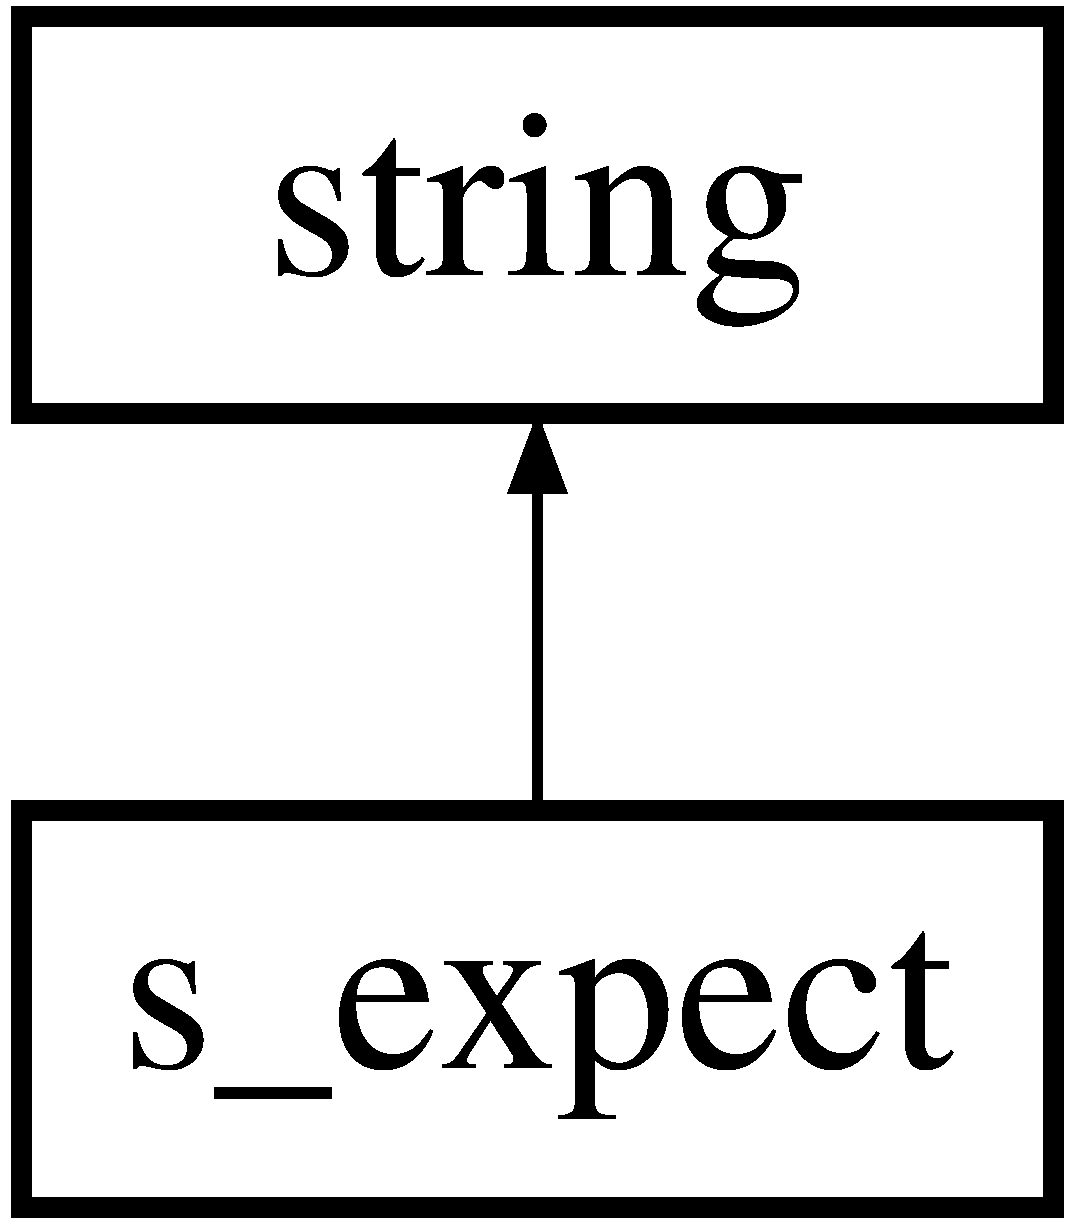
\includegraphics[height=2.000000cm]{classs__expect}
\end{center}
\end{figure}
\subsection*{Public Member Functions}
\begin{DoxyCompactItemize}
\item 
\mbox{\Hypertarget{classs__expect_ac20ef1b22d7cbc72ddbe05cc7abfae92}\label{classs__expect_ac20ef1b22d7cbc72ddbe05cc7abfae92}} 
{\bfseries s\+\_\+expect} (const char $\ast$s)
\item 
\mbox{\Hypertarget{classs__expect_aca6975249f49e68073d53a6d840f58e7}\label{classs__expect_aca6975249f49e68073d53a6d840f58e7}} 
{\bfseries s\+\_\+expect} (const std\+::string \&s)
\end{DoxyCompactItemize}
\subsection*{Friends}
\begin{DoxyCompactItemize}
\item 
\mbox{\Hypertarget{classs__expect_a4e0badbf124b3afd55ab2f134555d00e}\label{classs__expect_a4e0badbf124b3afd55ab2f134555d00e}} 
std\+::istream \& {\bfseries operator$>$$>$} (std\+::istream \&istr, \mbox{\hyperlink{classs__expect}{s\+\_\+expect}} \&\&s)
\item 
\mbox{\Hypertarget{classs__expect_a3fdcbe10442082a6e476d40576a80994}\label{classs__expect_a3fdcbe10442082a6e476d40576a80994}} 
std\+::istream \& {\bfseries operator$>$$>$} (std\+::istream \&\&istr, \mbox{\hyperlink{classs__expect}{s\+\_\+expect}} \&\&s)
\end{DoxyCompactItemize}


The documentation for this class was generated from the following file\+:\begin{DoxyCompactItemize}
\item 
\mbox{\hyperlink{utils_8h}{utils.\+h}}\end{DoxyCompactItemize}

\hypertarget{class_safe_msr_handle}{}\section{Safe\+Msr\+Handle Class Reference}
\label{class_safe_msr_handle}\index{Safe\+Msr\+Handle@{Safe\+Msr\+Handle}}
\subsection*{Public Member Functions}
\begin{DoxyCompactItemize}
\item 
\mbox{\Hypertarget{class_safe_msr_handle_af7a62cd143e86be1ef2d2f6d5f67fc30}\label{class_safe_msr_handle_af7a62cd143e86be1ef2d2f6d5f67fc30}} 
{\bfseries Safe\+Msr\+Handle} (uint32 core\+\_\+id)
\item 
\mbox{\Hypertarget{class_safe_msr_handle_af2ad27203ae5d1072ad8e1ca5d988ce5}\label{class_safe_msr_handle_af2ad27203ae5d1072ad8e1ca5d988ce5}} 
int32 {\bfseries read} (uint64 msr\+\_\+number, uint64 $\ast$value)
\item 
\mbox{\Hypertarget{class_safe_msr_handle_a252aa9dee867d8b8f787b1de007b49a7}\label{class_safe_msr_handle_a252aa9dee867d8b8f787b1de007b49a7}} 
int32 {\bfseries write} (uint64 msr\+\_\+number, uint64 value)
\item 
\mbox{\Hypertarget{class_safe_msr_handle_ae8735531f00abaaa17aac519c1e5360e}\label{class_safe_msr_handle_ae8735531f00abaaa17aac519c1e5360e}} 
int32 {\bfseries get\+Core\+Id} ()
\item 
\mbox{\Hypertarget{class_safe_msr_handle_a89f1431cde1d9e8ccd12c73cf6646cfd}\label{class_safe_msr_handle_a89f1431cde1d9e8ccd12c73cf6646cfd}} 
void {\bfseries lock} ()
\item 
\mbox{\Hypertarget{class_safe_msr_handle_af88c3d09575dab20ab68ce0267477e31}\label{class_safe_msr_handle_af88c3d09575dab20ab68ce0267477e31}} 
void {\bfseries unlock} ()
\end{DoxyCompactItemize}


The documentation for this class was generated from the following file\+:\begin{DoxyCompactItemize}
\item 
\mbox{\hyperlink{msr_8h}{msr.\+h}}\end{DoxyCompactItemize}

\hypertarget{structsample__t}{}\section{sample\+\_\+t Struct Reference}
\label{structsample__t}\index{sample\+\_\+t@{sample\+\_\+t}}
\subsection*{Public Attributes}
\begin{DoxyCompactItemize}
\item 
\mbox{\Hypertarget{structsample__t_adda6c294067fd623532a92a20266e75a}\label{structsample__t_adda6c294067fd623532a92a20266e75a}} 
\mbox{\hyperlink{struct_p_c_ie_events__t}{P\+C\+Ie\+Events\+\_\+t}} {\bfseries total}
\item 
\mbox{\Hypertarget{structsample__t_a88e5d78098bcfd43741b99ae218ad149}\label{structsample__t_a88e5d78098bcfd43741b99ae218ad149}} 
\mbox{\hyperlink{struct_p_c_ie_events__t}{P\+C\+Ie\+Events\+\_\+t}} {\bfseries miss}
\item 
\mbox{\Hypertarget{structsample__t_a2717168f76be8c4f1f46baf97231d9d6}\label{structsample__t_a2717168f76be8c4f1f46baf97231d9d6}} 
\mbox{\hyperlink{struct_p_c_ie_events__t}{P\+C\+Ie\+Events\+\_\+t}} {\bfseries hit}
\end{DoxyCompactItemize}


The documentation for this struct was generated from the following file\+:\begin{DoxyCompactItemize}
\item 
\mbox{\hyperlink{pcm-pcie_8cpp}{pcm-\/pcie.\+cpp}}\end{DoxyCompactItemize}

\hypertarget{class_p_c_m___util_1_1_mutex_1_1_scope}{}\section{P\+C\+M\+\_\+\+Util\+:\+:Mutex\+:\+:Scope Class Reference}
\label{class_p_c_m___util_1_1_mutex_1_1_scope}\index{P\+C\+M\+\_\+\+Util\+::\+Mutex\+::\+Scope@{P\+C\+M\+\_\+\+Util\+::\+Mutex\+::\+Scope}}
\subsection*{Public Member Functions}
\begin{DoxyCompactItemize}
\item 
\mbox{\Hypertarget{class_p_c_m___util_1_1_mutex_1_1_scope_aaf42d670b42a014200ad176d60d7c226}\label{class_p_c_m___util_1_1_mutex_1_1_scope_aaf42d670b42a014200ad176d60d7c226}} 
{\bfseries Scope} (\mbox{\hyperlink{class_p_c_m___util_1_1_mutex}{Mutex}} \&m\+\_\+)
\end{DoxyCompactItemize}


The documentation for this class was generated from the following file\+:\begin{DoxyCompactItemize}
\item 
mutex.\+h\end{DoxyCompactItemize}

\hypertarget{class_server_p_c_i_c_f_g_uncore}{}\section{Server\+P\+C\+I\+C\+F\+G\+Uncore Class Reference}
\label{class_server_p_c_i_c_f_g_uncore}\index{Server\+P\+C\+I\+C\+F\+G\+Uncore@{Server\+P\+C\+I\+C\+F\+G\+Uncore}}


Object to access uncore counters in a socket/processor with microarchitecture codename Sandy\+Bridge-\/\+EP (Jaketown) or Ivytown-\/\+EP or Ivytown-\/\+EX.  




{\ttfamily \#include $<$cpucounters.\+h$>$}

\subsection*{Public Member Functions}
\begin{DoxyCompactItemize}
\item 
\mbox{\hyperlink{class_server_p_c_i_c_f_g_uncore_a4e4176c31a041902805e16cc452016d3}{Server\+P\+C\+I\+C\+F\+G\+Uncore}} (uint32 socket\+\_\+, const \mbox{\hyperlink{class_p_c_m}{P\+CM}} $\ast$pcm)
\begin{DoxyCompactList}\small\item\em Initialize access data structures. \end{DoxyCompactList}\item 
\mbox{\Hypertarget{class_server_p_c_i_c_f_g_uncore_acd6e859dd5eaaadf97d2c59ae70ac4a7}\label{class_server_p_c_i_c_f_g_uncore_acd6e859dd5eaaadf97d2c59ae70ac4a7}} 
void \mbox{\hyperlink{class_server_p_c_i_c_f_g_uncore_acd6e859dd5eaaadf97d2c59ae70ac4a7}{program}} ()
\begin{DoxyCompactList}\small\item\em Program performance counters (disables programming power counters) \end{DoxyCompactList}\item 
\mbox{\Hypertarget{class_server_p_c_i_c_f_g_uncore_a214de12b52f2d5a7c9c33701dfc8eb85}\label{class_server_p_c_i_c_f_g_uncore_a214de12b52f2d5a7c9c33701dfc8eb85}} 
uint64 \mbox{\hyperlink{class_server_p_c_i_c_f_g_uncore_a214de12b52f2d5a7c9c33701dfc8eb85}{get\+Imc\+Reads}} ()
\begin{DoxyCompactList}\small\item\em Get the number of integrated controller reads (in cache lines) \end{DoxyCompactList}\item 
\mbox{\Hypertarget{class_server_p_c_i_c_f_g_uncore_a089f11fc46ab836884cc31b5b4ac08e3}\label{class_server_p_c_i_c_f_g_uncore_a089f11fc46ab836884cc31b5b4ac08e3}} 
uint64 \mbox{\hyperlink{class_server_p_c_i_c_f_g_uncore_a089f11fc46ab836884cc31b5b4ac08e3}{get\+Imc\+Writes}} ()
\begin{DoxyCompactList}\small\item\em Get the number of integrated controller writes (in cache lines) \end{DoxyCompactList}\item 
\mbox{\Hypertarget{class_server_p_c_i_c_f_g_uncore_a7a1fdecee105080d104bc7763d2fc06a}\label{class_server_p_c_i_c_f_g_uncore_a7a1fdecee105080d104bc7763d2fc06a}} 
uint64 \mbox{\hyperlink{class_server_p_c_i_c_f_g_uncore_a7a1fdecee105080d104bc7763d2fc06a}{get\+Edc\+Reads}} ()
\begin{DoxyCompactList}\small\item\em Get the number of cache lines read by E\+DC (embedded D\+R\+AM controller) \end{DoxyCompactList}\item 
\mbox{\Hypertarget{class_server_p_c_i_c_f_g_uncore_a1cdc322032c84f2eaeb36328c8d6ec0b}\label{class_server_p_c_i_c_f_g_uncore_a1cdc322032c84f2eaeb36328c8d6ec0b}} 
uint64 \mbox{\hyperlink{class_server_p_c_i_c_f_g_uncore_a1cdc322032c84f2eaeb36328c8d6ec0b}{get\+Edc\+Writes}} ()
\begin{DoxyCompactList}\small\item\em Get the number of cache lines written by E\+DC (embedded D\+R\+AM controller) \end{DoxyCompactList}\item 
uint64 \mbox{\hyperlink{class_server_p_c_i_c_f_g_uncore_abaeb0a56fa35ecbd0c092b733a1f923b}{get\+Incoming\+Data\+Flits}} (uint32 port)
\begin{DoxyCompactList}\small\item\em Get the number of incoming data flits to the socket through a port. \end{DoxyCompactList}\item 
uint64 \mbox{\hyperlink{class_server_p_c_i_c_f_g_uncore_ac318caa49f90d9cf3ee335656aa1f623}{get\+Outgoing\+Flits}} (uint32 port)
\begin{DoxyCompactList}\small\item\em Get the number of outgoing data and non-\/data or idle flits (depending on the architecture) from the socket through a port. \end{DoxyCompactList}\item 
void \mbox{\hyperlink{class_server_p_c_i_c_f_g_uncore_af53af91d9172cd124e455e500d6c5622}{program\+\_\+power\+\_\+metrics}} (int mc\+\_\+profile)
\begin{DoxyCompactList}\small\item\em Program power counters (disables programming performance counters) \end{DoxyCompactList}\item 
void \mbox{\hyperlink{class_server_p_c_i_c_f_g_uncore_a55caf03764268f7696fb8a2c8f3cc8f4}{program\+Server\+Uncore\+Memory\+Metrics}} (int rankA=-\/1, int rankB=-\/1)
\begin{DoxyCompactList}\small\item\em Program memory counters (disables programming performance counters) \end{DoxyCompactList}\item 
uint64 \mbox{\hyperlink{class_server_p_c_i_c_f_g_uncore_ae5bc4e8e1003ed74fdd3c641e6ac78a5}{get\+Q\+P\+I\+Clocks}} (uint32 port)
\begin{DoxyCompactList}\small\item\em Get number of Q\+PI LL clocks on a Q\+PI port. \end{DoxyCompactList}\item 
uint64 \mbox{\hyperlink{class_server_p_c_i_c_f_g_uncore_a7aaff7ae03c8189de550215cef3b39f7}{get\+Q\+P\+I\+L0p\+Tx\+Cycles}} (uint32 port)
\begin{DoxyCompactList}\small\item\em Get number cycles on a Q\+PI port when the link was in a power saving half-\/lane mode. \end{DoxyCompactList}\item 
uint64 \mbox{\hyperlink{class_server_p_c_i_c_f_g_uncore_aa7938ac7c048915bd256a3c5a5538701}{get\+U\+P\+I\+L0\+Tx\+Cycles}} (uint32 port)
\begin{DoxyCompactList}\small\item\em Get number cycles on a U\+PI port when the link was in a L0 mode (fully active) \end{DoxyCompactList}\item 
uint64 \mbox{\hyperlink{class_server_p_c_i_c_f_g_uncore_aa0ac63963af6105dd066f09beb923d17}{get\+Q\+P\+I\+L1\+Cycles}} (uint32 port)
\begin{DoxyCompactList}\small\item\em Get number cycles on a Q\+PI port when the link was in a power saving shutdown mode. \end{DoxyCompactList}\item 
uint64 \mbox{\hyperlink{class_server_p_c_i_c_f_g_uncore_a3b218ad26a3c6411754ed177427b2a80}{get\+D\+R\+A\+M\+Clocks}} (uint32 channel)
\begin{DoxyCompactList}\small\item\em Get number D\+R\+AM channel cycles. \end{DoxyCompactList}\item 
uint64 \mbox{\hyperlink{class_server_p_c_i_c_f_g_uncore_ad0138169a52467871058a4f810482e0e}{get\+M\+C\+D\+R\+A\+M\+Clocks}} (uint32 channel)
\begin{DoxyCompactList}\small\item\em Get number M\+C\+D\+R\+AM channel cycles. \end{DoxyCompactList}\item 
uint64 \mbox{\hyperlink{class_server_p_c_i_c_f_g_uncore_ad66687e98d1b74c145b79fedefc07d15}{get\+M\+C\+Counter}} (uint32 channel, uint32 \mbox{\hyperlink{structcounter}{counter}})
\begin{DoxyCompactList}\small\item\em Direct read of memory controller P\+MU counter (counter meaning depends on the programming\+: power/performance/etc) \end{DoxyCompactList}\item 
uint64 \mbox{\hyperlink{class_server_p_c_i_c_f_g_uncore_aa48e2113a37b0727b1dbe27c391ccd04}{get\+E\+D\+C\+Counter}} (uint32 channel, uint32 \mbox{\hyperlink{structcounter}{counter}})
\begin{DoxyCompactList}\small\item\em Direct read of embedded D\+R\+AM memory controller P\+MU counter (counter meaning depends on the programming\+: power/performance/etc) \end{DoxyCompactList}\item 
uint64 \mbox{\hyperlink{class_server_p_c_i_c_f_g_uncore_abcd9990a39fb245bb552e6cae4922305}{get\+Q\+P\+I\+L\+L\+Counter}} (uint32 port, uint32 \mbox{\hyperlink{structcounter}{counter}})
\begin{DoxyCompactList}\small\item\em Direct read of Q\+PI LL P\+MU counter (counter meaning depends on the programming\+: power/performance/etc) \end{DoxyCompactList}\item 
\mbox{\Hypertarget{class_server_p_c_i_c_f_g_uncore_ad4bda64cc17432d44ee8e380a735b795}\label{class_server_p_c_i_c_f_g_uncore_ad4bda64cc17432d44ee8e380a735b795}} 
void \mbox{\hyperlink{class_server_p_c_i_c_f_g_uncore_ad4bda64cc17432d44ee8e380a735b795}{freeze\+Counters}} ()
\begin{DoxyCompactList}\small\item\em Freezes event counting. \end{DoxyCompactList}\item 
\mbox{\Hypertarget{class_server_p_c_i_c_f_g_uncore_a379962b379f637f3b752f7fb4666c7e7}\label{class_server_p_c_i_c_f_g_uncore_a379962b379f637f3b752f7fb4666c7e7}} 
void \mbox{\hyperlink{class_server_p_c_i_c_f_g_uncore_a379962b379f637f3b752f7fb4666c7e7}{unfreeze\+Counters}} ()
\begin{DoxyCompactList}\small\item\em Unfreezes event counting. \end{DoxyCompactList}\item 
\mbox{\Hypertarget{class_server_p_c_i_c_f_g_uncore_a42a0e1343ab38371279bf9def8123419}\label{class_server_p_c_i_c_f_g_uncore_a42a0e1343ab38371279bf9def8123419}} 
uint64 \mbox{\hyperlink{class_server_p_c_i_c_f_g_uncore_a42a0e1343ab38371279bf9def8123419}{compute\+Q\+P\+I\+Speed}} (const uint32 ref\+\_\+core, const int cpumodel)
\begin{DoxyCompactList}\small\item\em Measures/computes the maximum theoretical Q\+PI link bandwidth speed in G\+Byte/seconds. \end{DoxyCompactList}\item 
\mbox{\Hypertarget{class_server_p_c_i_c_f_g_uncore_a91352764d2ab70889388f61d48852694}\label{class_server_p_c_i_c_f_g_uncore_a91352764d2ab70889388f61d48852694}} 
void \mbox{\hyperlink{class_server_p_c_i_c_f_g_uncore_a91352764d2ab70889388f61d48852694}{enable\+J\+K\+T\+Workaround}} (bool enable)
\begin{DoxyCompactList}\small\item\em Enable correct counting of various L\+LC events (with memory access perf penalty) \end{DoxyCompactList}\item 
\mbox{\Hypertarget{class_server_p_c_i_c_f_g_uncore_a5dc6e057441bbbbc3d396fe8e5d7cc2f}\label{class_server_p_c_i_c_f_g_uncore_a5dc6e057441bbbbc3d396fe8e5d7cc2f}} 
size\+\_\+t \mbox{\hyperlink{class_server_p_c_i_c_f_g_uncore_a5dc6e057441bbbbc3d396fe8e5d7cc2f}{get\+Num\+Q\+P\+I\+Ports}} () const
\begin{DoxyCompactList}\small\item\em Returns the number of detected Q\+PI ports. \end{DoxyCompactList}\item 
\mbox{\Hypertarget{class_server_p_c_i_c_f_g_uncore_ae3421871d5942f1835af1fe4c282950b}\label{class_server_p_c_i_c_f_g_uncore_ae3421871d5942f1835af1fe4c282950b}} 
uint64 \mbox{\hyperlink{class_server_p_c_i_c_f_g_uncore_ae3421871d5942f1835af1fe4c282950b}{get\+Q\+P\+I\+Link\+Speed}} (const uint32 link\+Nr) const
\begin{DoxyCompactList}\small\item\em Returns the speed of the Q\+PI link. \end{DoxyCompactList}\item 
\mbox{\Hypertarget{class_server_p_c_i_c_f_g_uncore_ab41eec236180d9d451fc1edc823dcc84}\label{class_server_p_c_i_c_f_g_uncore_ab41eec236180d9d451fc1edc823dcc84}} 
void \mbox{\hyperlink{class_server_p_c_i_c_f_g_uncore_ab41eec236180d9d451fc1edc823dcc84}{report\+Q\+P\+I\+Speed}} () const
\begin{DoxyCompactList}\small\item\em Print Q\+PI Speeds. \end{DoxyCompactList}\item 
\mbox{\Hypertarget{class_server_p_c_i_c_f_g_uncore_a70765cb7dc2f54fae3528e6f15c57f45}\label{class_server_p_c_i_c_f_g_uncore_a70765cb7dc2f54fae3528e6f15c57f45}} 
uint32 \mbox{\hyperlink{class_server_p_c_i_c_f_g_uncore_a70765cb7dc2f54fae3528e6f15c57f45}{get\+Num\+MC}} () const
\begin{DoxyCompactList}\small\item\em Returns the number of detected integrated memory controllers. \end{DoxyCompactList}\item 
\mbox{\Hypertarget{class_server_p_c_i_c_f_g_uncore_ab59fb235a87be897547b1c32534d1a5f}\label{class_server_p_c_i_c_f_g_uncore_ab59fb235a87be897547b1c32534d1a5f}} 
size\+\_\+t \mbox{\hyperlink{class_server_p_c_i_c_f_g_uncore_ab59fb235a87be897547b1c32534d1a5f}{get\+Num\+M\+C\+Channels}} () const
\begin{DoxyCompactList}\small\item\em Returns the total number of detected memory channels on all integrated memory controllers. \end{DoxyCompactList}\item 
\mbox{\Hypertarget{class_server_p_c_i_c_f_g_uncore_abc8b36bca06eaa243b1013ae19374c2c}\label{class_server_p_c_i_c_f_g_uncore_abc8b36bca06eaa243b1013ae19374c2c}} 
size\+\_\+t \mbox{\hyperlink{class_server_p_c_i_c_f_g_uncore_abc8b36bca06eaa243b1013ae19374c2c}{get\+Num\+E\+D\+C\+Channels}} () const
\begin{DoxyCompactList}\small\item\em Returns the total number of detected memory channels on all embedded D\+R\+AM controllers (E\+DC) \end{DoxyCompactList}\end{DoxyCompactItemize}


\subsection{Detailed Description}
Object to access uncore counters in a socket/processor with microarchitecture codename Sandy\+Bridge-\/\+EP (Jaketown) or Ivytown-\/\+EP or Ivytown-\/\+EX. 

\subsection{Constructor \& Destructor Documentation}
\mbox{\Hypertarget{class_server_p_c_i_c_f_g_uncore_a4e4176c31a041902805e16cc452016d3}\label{class_server_p_c_i_c_f_g_uncore_a4e4176c31a041902805e16cc452016d3}} 
\index{Server\+P\+C\+I\+C\+F\+G\+Uncore@{Server\+P\+C\+I\+C\+F\+G\+Uncore}!Server\+P\+C\+I\+C\+F\+G\+Uncore@{Server\+P\+C\+I\+C\+F\+G\+Uncore}}
\index{Server\+P\+C\+I\+C\+F\+G\+Uncore@{Server\+P\+C\+I\+C\+F\+G\+Uncore}!Server\+P\+C\+I\+C\+F\+G\+Uncore@{Server\+P\+C\+I\+C\+F\+G\+Uncore}}
\subsubsection{\texorpdfstring{Server\+P\+C\+I\+C\+F\+G\+Uncore()}{ServerPCICFGUncore()}}
{\footnotesize\ttfamily Server\+P\+C\+I\+C\+F\+G\+Uncore\+::\+Server\+P\+C\+I\+C\+F\+G\+Uncore (\begin{DoxyParamCaption}\item[{uint32}]{socket\+\_\+,  }\item[{const \mbox{\hyperlink{class_p_c_m}{P\+CM}} $\ast$}]{pcm }\end{DoxyParamCaption})}



Initialize access data structures. 


\begin{DoxyParams}{Parameters}
{\em socket\+\_\+} & socket id \\
\hline
{\em pcm} & pointer to \mbox{\hyperlink{class_p_c_m}{P\+CM}} instance \\
\hline
\end{DoxyParams}


\subsection{Member Function Documentation}
\mbox{\Hypertarget{class_server_p_c_i_c_f_g_uncore_a3b218ad26a3c6411754ed177427b2a80}\label{class_server_p_c_i_c_f_g_uncore_a3b218ad26a3c6411754ed177427b2a80}} 
\index{Server\+P\+C\+I\+C\+F\+G\+Uncore@{Server\+P\+C\+I\+C\+F\+G\+Uncore}!get\+D\+R\+A\+M\+Clocks@{get\+D\+R\+A\+M\+Clocks}}
\index{get\+D\+R\+A\+M\+Clocks@{get\+D\+R\+A\+M\+Clocks}!Server\+P\+C\+I\+C\+F\+G\+Uncore@{Server\+P\+C\+I\+C\+F\+G\+Uncore}}
\subsubsection{\texorpdfstring{get\+D\+R\+A\+M\+Clocks()}{getDRAMClocks()}}
{\footnotesize\ttfamily uint64 Server\+P\+C\+I\+C\+F\+G\+Uncore\+::get\+D\+R\+A\+M\+Clocks (\begin{DoxyParamCaption}\item[{uint32}]{channel }\end{DoxyParamCaption})}



Get number D\+R\+AM channel cycles. 


\begin{DoxyParams}{Parameters}
{\em channel} & channel number \\
\hline
\end{DoxyParams}
\mbox{\Hypertarget{class_server_p_c_i_c_f_g_uncore_aa48e2113a37b0727b1dbe27c391ccd04}\label{class_server_p_c_i_c_f_g_uncore_aa48e2113a37b0727b1dbe27c391ccd04}} 
\index{Server\+P\+C\+I\+C\+F\+G\+Uncore@{Server\+P\+C\+I\+C\+F\+G\+Uncore}!get\+E\+D\+C\+Counter@{get\+E\+D\+C\+Counter}}
\index{get\+E\+D\+C\+Counter@{get\+E\+D\+C\+Counter}!Server\+P\+C\+I\+C\+F\+G\+Uncore@{Server\+P\+C\+I\+C\+F\+G\+Uncore}}
\subsubsection{\texorpdfstring{get\+E\+D\+C\+Counter()}{getEDCCounter()}}
{\footnotesize\ttfamily uint64 Server\+P\+C\+I\+C\+F\+G\+Uncore\+::get\+E\+D\+C\+Counter (\begin{DoxyParamCaption}\item[{uint32}]{channel,  }\item[{uint32}]{counter }\end{DoxyParamCaption})}



Direct read of embedded D\+R\+AM memory controller P\+MU counter (counter meaning depends on the programming\+: power/performance/etc) 


\begin{DoxyParams}{Parameters}
{\em channel} & channel number \\
\hline
{\em counter} & counter number \\
\hline
\end{DoxyParams}
\mbox{\Hypertarget{class_server_p_c_i_c_f_g_uncore_abaeb0a56fa35ecbd0c092b733a1f923b}\label{class_server_p_c_i_c_f_g_uncore_abaeb0a56fa35ecbd0c092b733a1f923b}} 
\index{Server\+P\+C\+I\+C\+F\+G\+Uncore@{Server\+P\+C\+I\+C\+F\+G\+Uncore}!get\+Incoming\+Data\+Flits@{get\+Incoming\+Data\+Flits}}
\index{get\+Incoming\+Data\+Flits@{get\+Incoming\+Data\+Flits}!Server\+P\+C\+I\+C\+F\+G\+Uncore@{Server\+P\+C\+I\+C\+F\+G\+Uncore}}
\subsubsection{\texorpdfstring{get\+Incoming\+Data\+Flits()}{getIncomingDataFlits()}}
{\footnotesize\ttfamily uint64 Server\+P\+C\+I\+C\+F\+G\+Uncore\+::get\+Incoming\+Data\+Flits (\begin{DoxyParamCaption}\item[{uint32}]{port }\end{DoxyParamCaption})}



Get the number of incoming data flits to the socket through a port. 


\begin{DoxyParams}{Parameters}
{\em port} & Q\+PI port id \\
\hline
\end{DoxyParams}
\mbox{\Hypertarget{class_server_p_c_i_c_f_g_uncore_ad66687e98d1b74c145b79fedefc07d15}\label{class_server_p_c_i_c_f_g_uncore_ad66687e98d1b74c145b79fedefc07d15}} 
\index{Server\+P\+C\+I\+C\+F\+G\+Uncore@{Server\+P\+C\+I\+C\+F\+G\+Uncore}!get\+M\+C\+Counter@{get\+M\+C\+Counter}}
\index{get\+M\+C\+Counter@{get\+M\+C\+Counter}!Server\+P\+C\+I\+C\+F\+G\+Uncore@{Server\+P\+C\+I\+C\+F\+G\+Uncore}}
\subsubsection{\texorpdfstring{get\+M\+C\+Counter()}{getMCCounter()}}
{\footnotesize\ttfamily uint64 Server\+P\+C\+I\+C\+F\+G\+Uncore\+::get\+M\+C\+Counter (\begin{DoxyParamCaption}\item[{uint32}]{channel,  }\item[{uint32}]{counter }\end{DoxyParamCaption})}



Direct read of memory controller P\+MU counter (counter meaning depends on the programming\+: power/performance/etc) 


\begin{DoxyParams}{Parameters}
{\em channel} & channel number \\
\hline
{\em counter} & counter number \\
\hline
\end{DoxyParams}
\mbox{\Hypertarget{class_server_p_c_i_c_f_g_uncore_ad0138169a52467871058a4f810482e0e}\label{class_server_p_c_i_c_f_g_uncore_ad0138169a52467871058a4f810482e0e}} 
\index{Server\+P\+C\+I\+C\+F\+G\+Uncore@{Server\+P\+C\+I\+C\+F\+G\+Uncore}!get\+M\+C\+D\+R\+A\+M\+Clocks@{get\+M\+C\+D\+R\+A\+M\+Clocks}}
\index{get\+M\+C\+D\+R\+A\+M\+Clocks@{get\+M\+C\+D\+R\+A\+M\+Clocks}!Server\+P\+C\+I\+C\+F\+G\+Uncore@{Server\+P\+C\+I\+C\+F\+G\+Uncore}}
\subsubsection{\texorpdfstring{get\+M\+C\+D\+R\+A\+M\+Clocks()}{getMCDRAMClocks()}}
{\footnotesize\ttfamily uint64 Server\+P\+C\+I\+C\+F\+G\+Uncore\+::get\+M\+C\+D\+R\+A\+M\+Clocks (\begin{DoxyParamCaption}\item[{uint32}]{channel }\end{DoxyParamCaption})}



Get number M\+C\+D\+R\+AM channel cycles. 


\begin{DoxyParams}{Parameters}
{\em channel} & channel number \\
\hline
\end{DoxyParams}
\mbox{\Hypertarget{class_server_p_c_i_c_f_g_uncore_ac318caa49f90d9cf3ee335656aa1f623}\label{class_server_p_c_i_c_f_g_uncore_ac318caa49f90d9cf3ee335656aa1f623}} 
\index{Server\+P\+C\+I\+C\+F\+G\+Uncore@{Server\+P\+C\+I\+C\+F\+G\+Uncore}!get\+Outgoing\+Flits@{get\+Outgoing\+Flits}}
\index{get\+Outgoing\+Flits@{get\+Outgoing\+Flits}!Server\+P\+C\+I\+C\+F\+G\+Uncore@{Server\+P\+C\+I\+C\+F\+G\+Uncore}}
\subsubsection{\texorpdfstring{get\+Outgoing\+Flits()}{getOutgoingFlits()}}
{\footnotesize\ttfamily uint64 Server\+P\+C\+I\+C\+F\+G\+Uncore\+::get\+Outgoing\+Flits (\begin{DoxyParamCaption}\item[{uint32}]{port }\end{DoxyParamCaption})}



Get the number of outgoing data and non-\/data or idle flits (depending on the architecture) from the socket through a port. 


\begin{DoxyParams}{Parameters}
{\em port} & Q\+PI port id \\
\hline
\end{DoxyParams}
\mbox{\Hypertarget{class_server_p_c_i_c_f_g_uncore_ae5bc4e8e1003ed74fdd3c641e6ac78a5}\label{class_server_p_c_i_c_f_g_uncore_ae5bc4e8e1003ed74fdd3c641e6ac78a5}} 
\index{Server\+P\+C\+I\+C\+F\+G\+Uncore@{Server\+P\+C\+I\+C\+F\+G\+Uncore}!get\+Q\+P\+I\+Clocks@{get\+Q\+P\+I\+Clocks}}
\index{get\+Q\+P\+I\+Clocks@{get\+Q\+P\+I\+Clocks}!Server\+P\+C\+I\+C\+F\+G\+Uncore@{Server\+P\+C\+I\+C\+F\+G\+Uncore}}
\subsubsection{\texorpdfstring{get\+Q\+P\+I\+Clocks()}{getQPIClocks()}}
{\footnotesize\ttfamily uint64 Server\+P\+C\+I\+C\+F\+G\+Uncore\+::get\+Q\+P\+I\+Clocks (\begin{DoxyParamCaption}\item[{uint32}]{port }\end{DoxyParamCaption})}



Get number of Q\+PI LL clocks on a Q\+PI port. 


\begin{DoxyParams}{Parameters}
{\em port} & Q\+PI port number \\
\hline
\end{DoxyParams}
\mbox{\Hypertarget{class_server_p_c_i_c_f_g_uncore_a7aaff7ae03c8189de550215cef3b39f7}\label{class_server_p_c_i_c_f_g_uncore_a7aaff7ae03c8189de550215cef3b39f7}} 
\index{Server\+P\+C\+I\+C\+F\+G\+Uncore@{Server\+P\+C\+I\+C\+F\+G\+Uncore}!get\+Q\+P\+I\+L0p\+Tx\+Cycles@{get\+Q\+P\+I\+L0p\+Tx\+Cycles}}
\index{get\+Q\+P\+I\+L0p\+Tx\+Cycles@{get\+Q\+P\+I\+L0p\+Tx\+Cycles}!Server\+P\+C\+I\+C\+F\+G\+Uncore@{Server\+P\+C\+I\+C\+F\+G\+Uncore}}
\subsubsection{\texorpdfstring{get\+Q\+P\+I\+L0p\+Tx\+Cycles()}{getQPIL0pTxCycles()}}
{\footnotesize\ttfamily uint64 Server\+P\+C\+I\+C\+F\+G\+Uncore\+::get\+Q\+P\+I\+L0p\+Tx\+Cycles (\begin{DoxyParamCaption}\item[{uint32}]{port }\end{DoxyParamCaption})}



Get number cycles on a Q\+PI port when the link was in a power saving half-\/lane mode. 


\begin{DoxyParams}{Parameters}
{\em port} & Q\+PI port number \\
\hline
\end{DoxyParams}
\mbox{\Hypertarget{class_server_p_c_i_c_f_g_uncore_aa0ac63963af6105dd066f09beb923d17}\label{class_server_p_c_i_c_f_g_uncore_aa0ac63963af6105dd066f09beb923d17}} 
\index{Server\+P\+C\+I\+C\+F\+G\+Uncore@{Server\+P\+C\+I\+C\+F\+G\+Uncore}!get\+Q\+P\+I\+L1\+Cycles@{get\+Q\+P\+I\+L1\+Cycles}}
\index{get\+Q\+P\+I\+L1\+Cycles@{get\+Q\+P\+I\+L1\+Cycles}!Server\+P\+C\+I\+C\+F\+G\+Uncore@{Server\+P\+C\+I\+C\+F\+G\+Uncore}}
\subsubsection{\texorpdfstring{get\+Q\+P\+I\+L1\+Cycles()}{getQPIL1Cycles()}}
{\footnotesize\ttfamily uint64 Server\+P\+C\+I\+C\+F\+G\+Uncore\+::get\+Q\+P\+I\+L1\+Cycles (\begin{DoxyParamCaption}\item[{uint32}]{port }\end{DoxyParamCaption})}



Get number cycles on a Q\+PI port when the link was in a power saving shutdown mode. 


\begin{DoxyParams}{Parameters}
{\em port} & Q\+PI port number \\
\hline
\end{DoxyParams}
\mbox{\Hypertarget{class_server_p_c_i_c_f_g_uncore_abcd9990a39fb245bb552e6cae4922305}\label{class_server_p_c_i_c_f_g_uncore_abcd9990a39fb245bb552e6cae4922305}} 
\index{Server\+P\+C\+I\+C\+F\+G\+Uncore@{Server\+P\+C\+I\+C\+F\+G\+Uncore}!get\+Q\+P\+I\+L\+L\+Counter@{get\+Q\+P\+I\+L\+L\+Counter}}
\index{get\+Q\+P\+I\+L\+L\+Counter@{get\+Q\+P\+I\+L\+L\+Counter}!Server\+P\+C\+I\+C\+F\+G\+Uncore@{Server\+P\+C\+I\+C\+F\+G\+Uncore}}
\subsubsection{\texorpdfstring{get\+Q\+P\+I\+L\+L\+Counter()}{getQPILLCounter()}}
{\footnotesize\ttfamily uint64 Server\+P\+C\+I\+C\+F\+G\+Uncore\+::get\+Q\+P\+I\+L\+L\+Counter (\begin{DoxyParamCaption}\item[{uint32}]{port,  }\item[{uint32}]{counter }\end{DoxyParamCaption})}



Direct read of Q\+PI LL P\+MU counter (counter meaning depends on the programming\+: power/performance/etc) 


\begin{DoxyParams}{Parameters}
{\em port} & port number \\
\hline
{\em counter} & counter number \\
\hline
\end{DoxyParams}
\mbox{\Hypertarget{class_server_p_c_i_c_f_g_uncore_aa7938ac7c048915bd256a3c5a5538701}\label{class_server_p_c_i_c_f_g_uncore_aa7938ac7c048915bd256a3c5a5538701}} 
\index{Server\+P\+C\+I\+C\+F\+G\+Uncore@{Server\+P\+C\+I\+C\+F\+G\+Uncore}!get\+U\+P\+I\+L0\+Tx\+Cycles@{get\+U\+P\+I\+L0\+Tx\+Cycles}}
\index{get\+U\+P\+I\+L0\+Tx\+Cycles@{get\+U\+P\+I\+L0\+Tx\+Cycles}!Server\+P\+C\+I\+C\+F\+G\+Uncore@{Server\+P\+C\+I\+C\+F\+G\+Uncore}}
\subsubsection{\texorpdfstring{get\+U\+P\+I\+L0\+Tx\+Cycles()}{getUPIL0TxCycles()}}
{\footnotesize\ttfamily uint64 Server\+P\+C\+I\+C\+F\+G\+Uncore\+::get\+U\+P\+I\+L0\+Tx\+Cycles (\begin{DoxyParamCaption}\item[{uint32}]{port }\end{DoxyParamCaption})}



Get number cycles on a U\+PI port when the link was in a L0 mode (fully active) 


\begin{DoxyParams}{Parameters}
{\em port} & U\+PI port number \\
\hline
\end{DoxyParams}
\mbox{\Hypertarget{class_server_p_c_i_c_f_g_uncore_af53af91d9172cd124e455e500d6c5622}\label{class_server_p_c_i_c_f_g_uncore_af53af91d9172cd124e455e500d6c5622}} 
\index{Server\+P\+C\+I\+C\+F\+G\+Uncore@{Server\+P\+C\+I\+C\+F\+G\+Uncore}!program\+\_\+power\+\_\+metrics@{program\+\_\+power\+\_\+metrics}}
\index{program\+\_\+power\+\_\+metrics@{program\+\_\+power\+\_\+metrics}!Server\+P\+C\+I\+C\+F\+G\+Uncore@{Server\+P\+C\+I\+C\+F\+G\+Uncore}}
\subsubsection{\texorpdfstring{program\+\_\+power\+\_\+metrics()}{program\_power\_metrics()}}
{\footnotesize\ttfamily void Server\+P\+C\+I\+C\+F\+G\+Uncore\+::program\+\_\+power\+\_\+metrics (\begin{DoxyParamCaption}\item[{int}]{mc\+\_\+profile }\end{DoxyParamCaption})}



Program power counters (disables programming performance counters) 


\begin{DoxyParams}{Parameters}
{\em mc\+\_\+profile} & memory controller measurement profile. See description of profiles in pcm-\/power.\+cpp \\
\hline
\end{DoxyParams}
\mbox{\Hypertarget{class_server_p_c_i_c_f_g_uncore_a55caf03764268f7696fb8a2c8f3cc8f4}\label{class_server_p_c_i_c_f_g_uncore_a55caf03764268f7696fb8a2c8f3cc8f4}} 
\index{Server\+P\+C\+I\+C\+F\+G\+Uncore@{Server\+P\+C\+I\+C\+F\+G\+Uncore}!program\+Server\+Uncore\+Memory\+Metrics@{program\+Server\+Uncore\+Memory\+Metrics}}
\index{program\+Server\+Uncore\+Memory\+Metrics@{program\+Server\+Uncore\+Memory\+Metrics}!Server\+P\+C\+I\+C\+F\+G\+Uncore@{Server\+P\+C\+I\+C\+F\+G\+Uncore}}
\subsubsection{\texorpdfstring{program\+Server\+Uncore\+Memory\+Metrics()}{programServerUncoreMemoryMetrics()}}
{\footnotesize\ttfamily void Server\+P\+C\+I\+C\+F\+G\+Uncore\+::program\+Server\+Uncore\+Memory\+Metrics (\begin{DoxyParamCaption}\item[{int}]{rankA = {\ttfamily -\/1},  }\item[{int}]{rankB = {\ttfamily -\/1} }\end{DoxyParamCaption})}



Program memory counters (disables programming performance counters) 


\begin{DoxyParams}{Parameters}
{\em rankA} & count D\+I\+MM rank1 statistics (disables memory channel monitoring) \\
\hline
{\em rankB} & count D\+I\+MM rank2 statistics (disables memory channel monitoring) \\
\hline
\end{DoxyParams}


The documentation for this class was generated from the following files\+:\begin{DoxyCompactItemize}
\item 
\mbox{\hyperlink{cpucounters_8h}{cpucounters.\+h}}\item 
\mbox{\hyperlink{cpucounters_8cpp}{cpucounters.\+cpp}}\end{DoxyCompactItemize}

\hypertarget{class_server_uncore_power_state}{}\section{Server\+Uncore\+Power\+State Class Reference}
\label{class_server_uncore_power_state}\index{Server\+Uncore\+Power\+State@{Server\+Uncore\+Power\+State}}


Server uncore power counter state.  




{\ttfamily \#include $<$cpucounters.\+h$>$}

Inheritance diagram for Server\+Uncore\+Power\+State\+:\begin{figure}[H]
\begin{center}
\leavevmode
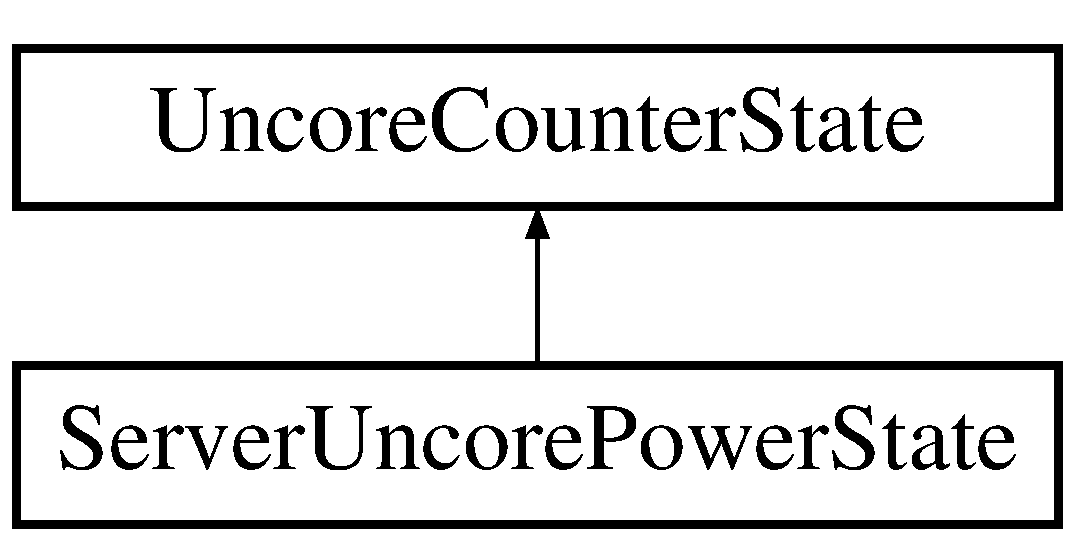
\includegraphics[height=2.000000cm]{class_server_uncore_power_state}
\end{center}
\end{figure}
\subsection*{Public Member Functions}
\begin{DoxyCompactItemize}
\item 
\mbox{\Hypertarget{class_server_uncore_power_state_a0d500b1b06aac2fd0271574aa9c8f461}\label{class_server_uncore_power_state_a0d500b1b06aac2fd0271574aa9c8f461}} 
int32 \mbox{\hyperlink{class_server_uncore_power_state_a0d500b1b06aac2fd0271574aa9c8f461}{get\+Package\+Thermal\+Headroom}} () const
\begin{DoxyCompactList}\small\item\em Returns current thermal headroom below Tj\+Max. \end{DoxyCompactList}\end{DoxyCompactItemize}
\subsection*{Friends}
\begin{DoxyCompactItemize}
\item 
\mbox{\Hypertarget{class_server_uncore_power_state_ab5f56d2e95ba3daf52c17b8a1d356d64}\label{class_server_uncore_power_state_ab5f56d2e95ba3daf52c17b8a1d356d64}} 
class {\bfseries P\+CM}
\item 
{\footnotesize template$<$class Counter\+State\+Type $>$ }\\uint64 \mbox{\hyperlink{class_server_uncore_power_state_af7d9ba0936d7c305d0cc6c2db296a336}{get\+Q\+P\+I\+Clocks}} (uint32 port, const Counter\+State\+Type \&before, const Counter\+State\+Type \&after)
\begin{DoxyCompactList}\small\item\em Returns Q\+PI LL clock ticks. \end{DoxyCompactList}\item 
{\footnotesize template$<$class Counter\+State\+Type $>$ }\\uint64 \mbox{\hyperlink{class_server_uncore_power_state_acdac5d9d7a5a6496d90b0681badc26b3}{get\+Q\+P\+I\+L0p\+Tx\+Cycles}} (uint32 port, const Counter\+State\+Type \&before, const Counter\+State\+Type \&after)
\begin{DoxyCompactList}\small\item\em Returns the number of Q\+PI cycles in power saving half-\/lane mode. \end{DoxyCompactList}\item 
{\footnotesize template$<$class Counter\+State\+Type $>$ }\\uint64 \mbox{\hyperlink{class_server_uncore_power_state_a580ae4e465d0f8dd93935ad7af28c095}{get\+Q\+P\+I\+L1\+Cycles}} (uint32 port, const Counter\+State\+Type \&before, const Counter\+State\+Type \&after)
\begin{DoxyCompactList}\small\item\em Returns the number of Q\+PI cycles in power saving shutdown mode. \end{DoxyCompactList}\item 
{\footnotesize template$<$class Counter\+State\+Type $>$ }\\uint64 \mbox{\hyperlink{class_server_uncore_power_state_aeb1baf7feb391c0512dc378a9fd66a17}{get\+D\+R\+A\+M\+Clocks}} (uint32 channel, const Counter\+State\+Type \&before, const Counter\+State\+Type \&after)
\begin{DoxyCompactList}\small\item\em Returns D\+R\+AM clock ticks. \end{DoxyCompactList}\item 
{\footnotesize template$<$class Counter\+State\+Type $>$ }\\uint64 \mbox{\hyperlink{class_server_uncore_power_state_a1615063ac14cde3ace1a91bfb349f3f9}{get\+M\+C\+D\+R\+A\+M\+Clocks}} (uint32 channel, const Counter\+State\+Type \&before, const Counter\+State\+Type \&after)
\begin{DoxyCompactList}\small\item\em Returns M\+C\+D\+R\+AM clock ticks. \end{DoxyCompactList}\item 
{\footnotesize template$<$class Counter\+State\+Type $>$ }\\uint64 \mbox{\hyperlink{class_server_uncore_power_state_aed082cc97dbad35e1633823e582afa0f}{get\+M\+C\+Counter}} (uint32 channel, uint32 \mbox{\hyperlink{structcounter}{counter}}, const Counter\+State\+Type \&before, const Counter\+State\+Type \&after)
\begin{DoxyCompactList}\small\item\em Direct read of memory controller P\+MU counter (counter meaning depends on the programming\+: power/performance/etc) \end{DoxyCompactList}\item 
{\footnotesize template$<$class Counter\+State\+Type $>$ }\\uint64 \mbox{\hyperlink{class_server_uncore_power_state_a996fd8a127111e06540302cf9ccb24a7}{get\+E\+D\+C\+Counter}} (uint32 channel, uint32 \mbox{\hyperlink{structcounter}{counter}}, const Counter\+State\+Type \&before, const Counter\+State\+Type \&after)
\begin{DoxyCompactList}\small\item\em Direct read of embedded D\+R\+AM memory controller counter (counter meaning depends on the programming\+: power/performance/etc) \end{DoxyCompactList}\item 
{\footnotesize template$<$class Counter\+State\+Type $>$ }\\uint64 \mbox{\hyperlink{class_server_uncore_power_state_a3c424ad42d2439410d6ffc371335573d}{get\+P\+C\+U\+Counter}} (uint32 \mbox{\hyperlink{structcounter}{counter}}, const Counter\+State\+Type \&before, const Counter\+State\+Type \&after)
\begin{DoxyCompactList}\small\item\em Direct read of power control unit P\+MU counter (counter meaning depends on the programming\+: power/performance/etc) \end{DoxyCompactList}\item 
{\footnotesize template$<$class Counter\+State\+Type $>$ }\\uint64 \mbox{\hyperlink{class_server_uncore_power_state_a054b949f09283093e1923affa4e58ae8}{get\+Consumed\+Energy}} (const Counter\+State\+Type \&before, const Counter\+State\+Type \&after)
\begin{DoxyCompactList}\small\item\em Returns energy consumed by processor, exclusing D\+R\+AM (measured in internal units) \end{DoxyCompactList}\item 
{\footnotesize template$<$class Counter\+State\+Type $>$ }\\uint64 \mbox{\hyperlink{class_server_uncore_power_state_a71af0766460ef7dd3d138ec0d0924eda}{get\+D\+R\+A\+M\+Consumed\+Energy}} (const Counter\+State\+Type \&before, const Counter\+State\+Type \&after)
\begin{DoxyCompactList}\small\item\em Returns energy consumed by D\+R\+AM (measured in internal units) \end{DoxyCompactList}\item 
{\footnotesize template$<$class Counter\+State\+Type $>$ }\\uint64 \mbox{\hyperlink{class_server_uncore_power_state_a45cf07a8d3ce2c48968842554a3854f9}{get\+Invariant\+T\+SC}} (const Counter\+State\+Type \&before, const Counter\+State\+Type \&after)
\begin{DoxyCompactList}\small\item\em Computes number of invariant time stamp counter ticks. \end{DoxyCompactList}\end{DoxyCompactItemize}
\subsection*{Additional Inherited Members}


\subsection{Detailed Description}
Server uncore power counter state. 

\subsection{Friends And Related Function Documentation}
\mbox{\Hypertarget{class_server_uncore_power_state_a054b949f09283093e1923affa4e58ae8}\label{class_server_uncore_power_state_a054b949f09283093e1923affa4e58ae8}} 
\index{Server\+Uncore\+Power\+State@{Server\+Uncore\+Power\+State}!get\+Consumed\+Energy@{get\+Consumed\+Energy}}
\index{get\+Consumed\+Energy@{get\+Consumed\+Energy}!Server\+Uncore\+Power\+State@{Server\+Uncore\+Power\+State}}
\subsubsection{\texorpdfstring{get\+Consumed\+Energy}{getConsumedEnergy}}
{\footnotesize\ttfamily template$<$class Counter\+State\+Type $>$ \\
uint64 get\+Consumed\+Energy (\begin{DoxyParamCaption}\item[{const Counter\+State\+Type \&}]{before,  }\item[{const Counter\+State\+Type \&}]{after }\end{DoxyParamCaption})\hspace{0.3cm}{\ttfamily [friend]}}



Returns energy consumed by processor, exclusing D\+R\+AM (measured in internal units) 


\begin{DoxyParams}{Parameters}
{\em before} & C\+PU counter state before the experiment \\
\hline
{\em after} & C\+PU counter state after the experiment \\
\hline
\end{DoxyParams}
\mbox{\Hypertarget{class_server_uncore_power_state_aeb1baf7feb391c0512dc378a9fd66a17}\label{class_server_uncore_power_state_aeb1baf7feb391c0512dc378a9fd66a17}} 
\index{Server\+Uncore\+Power\+State@{Server\+Uncore\+Power\+State}!get\+D\+R\+A\+M\+Clocks@{get\+D\+R\+A\+M\+Clocks}}
\index{get\+D\+R\+A\+M\+Clocks@{get\+D\+R\+A\+M\+Clocks}!Server\+Uncore\+Power\+State@{Server\+Uncore\+Power\+State}}
\subsubsection{\texorpdfstring{get\+D\+R\+A\+M\+Clocks}{getDRAMClocks}}
{\footnotesize\ttfamily template$<$class Counter\+State\+Type $>$ \\
uint64 get\+D\+R\+A\+M\+Clocks (\begin{DoxyParamCaption}\item[{uint32}]{channel,  }\item[{const Counter\+State\+Type \&}]{before,  }\item[{const Counter\+State\+Type \&}]{after }\end{DoxyParamCaption})\hspace{0.3cm}{\ttfamily [friend]}}



Returns D\+R\+AM clock ticks. 


\begin{DoxyParams}{Parameters}
{\em channel} & D\+R\+AM channel number \\
\hline
{\em before} & C\+PU counter state before the experiment \\
\hline
{\em after} & C\+PU counter state after the experiment \\
\hline
\end{DoxyParams}
\mbox{\Hypertarget{class_server_uncore_power_state_a71af0766460ef7dd3d138ec0d0924eda}\label{class_server_uncore_power_state_a71af0766460ef7dd3d138ec0d0924eda}} 
\index{Server\+Uncore\+Power\+State@{Server\+Uncore\+Power\+State}!get\+D\+R\+A\+M\+Consumed\+Energy@{get\+D\+R\+A\+M\+Consumed\+Energy}}
\index{get\+D\+R\+A\+M\+Consumed\+Energy@{get\+D\+R\+A\+M\+Consumed\+Energy}!Server\+Uncore\+Power\+State@{Server\+Uncore\+Power\+State}}
\subsubsection{\texorpdfstring{get\+D\+R\+A\+M\+Consumed\+Energy}{getDRAMConsumedEnergy}}
{\footnotesize\ttfamily template$<$class Counter\+State\+Type $>$ \\
uint64 get\+D\+R\+A\+M\+Consumed\+Energy (\begin{DoxyParamCaption}\item[{const Counter\+State\+Type \&}]{before,  }\item[{const Counter\+State\+Type \&}]{after }\end{DoxyParamCaption})\hspace{0.3cm}{\ttfamily [friend]}}



Returns energy consumed by D\+R\+AM (measured in internal units) 


\begin{DoxyParams}{Parameters}
{\em before} & C\+PU counter state before the experiment \\
\hline
{\em after} & C\+PU counter state after the experiment \\
\hline
\end{DoxyParams}
\mbox{\Hypertarget{class_server_uncore_power_state_a996fd8a127111e06540302cf9ccb24a7}\label{class_server_uncore_power_state_a996fd8a127111e06540302cf9ccb24a7}} 
\index{Server\+Uncore\+Power\+State@{Server\+Uncore\+Power\+State}!get\+E\+D\+C\+Counter@{get\+E\+D\+C\+Counter}}
\index{get\+E\+D\+C\+Counter@{get\+E\+D\+C\+Counter}!Server\+Uncore\+Power\+State@{Server\+Uncore\+Power\+State}}
\subsubsection{\texorpdfstring{get\+E\+D\+C\+Counter}{getEDCCounter}}
{\footnotesize\ttfamily template$<$class Counter\+State\+Type $>$ \\
uint64 get\+E\+D\+C\+Counter (\begin{DoxyParamCaption}\item[{uint32}]{channel,  }\item[{uint32}]{counter,  }\item[{const Counter\+State\+Type \&}]{before,  }\item[{const Counter\+State\+Type \&}]{after }\end{DoxyParamCaption})\hspace{0.3cm}{\ttfamily [friend]}}



Direct read of embedded D\+R\+AM memory controller counter (counter meaning depends on the programming\+: power/performance/etc) 


\begin{DoxyParams}{Parameters}
{\em counter} & counter number \\
\hline
{\em channel} & channel number \\
\hline
{\em before} & C\+PU counter state before the experiment \\
\hline
{\em after} & C\+PU counter state after the experiment \\
\hline
\end{DoxyParams}
\mbox{\Hypertarget{class_server_uncore_power_state_a45cf07a8d3ce2c48968842554a3854f9}\label{class_server_uncore_power_state_a45cf07a8d3ce2c48968842554a3854f9}} 
\index{Server\+Uncore\+Power\+State@{Server\+Uncore\+Power\+State}!get\+Invariant\+T\+SC@{get\+Invariant\+T\+SC}}
\index{get\+Invariant\+T\+SC@{get\+Invariant\+T\+SC}!Server\+Uncore\+Power\+State@{Server\+Uncore\+Power\+State}}
\subsubsection{\texorpdfstring{get\+Invariant\+T\+SC}{getInvariantTSC}}
{\footnotesize\ttfamily template$<$class Counter\+State\+Type $>$ \\
uint64 get\+Invariant\+T\+SC (\begin{DoxyParamCaption}\item[{const Counter\+State\+Type \&}]{before,  }\item[{const Counter\+State\+Type \&}]{after }\end{DoxyParamCaption})\hspace{0.3cm}{\ttfamily [friend]}}



Computes number of invariant time stamp counter ticks. 

This counter counts irrespectively of C-\/, P-\/ or T-\/states


\begin{DoxyParams}{Parameters}
{\em before} & C\+PU counter state before the experiment \\
\hline
{\em after} & C\+PU counter state after the experiment \\
\hline
\end{DoxyParams}
\begin{DoxyReturn}{Returns}
number of time stamp counter ticks 
\end{DoxyReturn}
\mbox{\Hypertarget{class_server_uncore_power_state_aed082cc97dbad35e1633823e582afa0f}\label{class_server_uncore_power_state_aed082cc97dbad35e1633823e582afa0f}} 
\index{Server\+Uncore\+Power\+State@{Server\+Uncore\+Power\+State}!get\+M\+C\+Counter@{get\+M\+C\+Counter}}
\index{get\+M\+C\+Counter@{get\+M\+C\+Counter}!Server\+Uncore\+Power\+State@{Server\+Uncore\+Power\+State}}
\subsubsection{\texorpdfstring{get\+M\+C\+Counter}{getMCCounter}}
{\footnotesize\ttfamily template$<$class Counter\+State\+Type $>$ \\
uint64 get\+M\+C\+Counter (\begin{DoxyParamCaption}\item[{uint32}]{channel,  }\item[{uint32}]{counter,  }\item[{const Counter\+State\+Type \&}]{before,  }\item[{const Counter\+State\+Type \&}]{after }\end{DoxyParamCaption})\hspace{0.3cm}{\ttfamily [friend]}}



Direct read of memory controller P\+MU counter (counter meaning depends on the programming\+: power/performance/etc) 


\begin{DoxyParams}{Parameters}
{\em counter} & counter number \\
\hline
{\em channel} & channel number \\
\hline
{\em before} & C\+PU counter state before the experiment \\
\hline
{\em after} & C\+PU counter state after the experiment \\
\hline
\end{DoxyParams}
\mbox{\Hypertarget{class_server_uncore_power_state_a1615063ac14cde3ace1a91bfb349f3f9}\label{class_server_uncore_power_state_a1615063ac14cde3ace1a91bfb349f3f9}} 
\index{Server\+Uncore\+Power\+State@{Server\+Uncore\+Power\+State}!get\+M\+C\+D\+R\+A\+M\+Clocks@{get\+M\+C\+D\+R\+A\+M\+Clocks}}
\index{get\+M\+C\+D\+R\+A\+M\+Clocks@{get\+M\+C\+D\+R\+A\+M\+Clocks}!Server\+Uncore\+Power\+State@{Server\+Uncore\+Power\+State}}
\subsubsection{\texorpdfstring{get\+M\+C\+D\+R\+A\+M\+Clocks}{getMCDRAMClocks}}
{\footnotesize\ttfamily template$<$class Counter\+State\+Type $>$ \\
uint64 get\+M\+C\+D\+R\+A\+M\+Clocks (\begin{DoxyParamCaption}\item[{uint32}]{channel,  }\item[{const Counter\+State\+Type \&}]{before,  }\item[{const Counter\+State\+Type \&}]{after }\end{DoxyParamCaption})\hspace{0.3cm}{\ttfamily [friend]}}



Returns M\+C\+D\+R\+AM clock ticks. 


\begin{DoxyParams}{Parameters}
{\em channel} & M\+C\+D\+R\+AM channel number \\
\hline
{\em before} & C\+PU counter state before the experiment \\
\hline
{\em after} & C\+PU counter state after the experiment \\
\hline
\end{DoxyParams}
\mbox{\Hypertarget{class_server_uncore_power_state_a3c424ad42d2439410d6ffc371335573d}\label{class_server_uncore_power_state_a3c424ad42d2439410d6ffc371335573d}} 
\index{Server\+Uncore\+Power\+State@{Server\+Uncore\+Power\+State}!get\+P\+C\+U\+Counter@{get\+P\+C\+U\+Counter}}
\index{get\+P\+C\+U\+Counter@{get\+P\+C\+U\+Counter}!Server\+Uncore\+Power\+State@{Server\+Uncore\+Power\+State}}
\subsubsection{\texorpdfstring{get\+P\+C\+U\+Counter}{getPCUCounter}}
{\footnotesize\ttfamily template$<$class Counter\+State\+Type $>$ \\
uint64 get\+P\+C\+U\+Counter (\begin{DoxyParamCaption}\item[{uint32}]{counter,  }\item[{const Counter\+State\+Type \&}]{before,  }\item[{const Counter\+State\+Type \&}]{after }\end{DoxyParamCaption})\hspace{0.3cm}{\ttfamily [friend]}}



Direct read of power control unit P\+MU counter (counter meaning depends on the programming\+: power/performance/etc) 


\begin{DoxyParams}{Parameters}
{\em counter} & counter number \\
\hline
{\em before} & C\+PU counter state before the experiment \\
\hline
{\em after} & C\+PU counter state after the experiment \\
\hline
\end{DoxyParams}
\mbox{\Hypertarget{class_server_uncore_power_state_af7d9ba0936d7c305d0cc6c2db296a336}\label{class_server_uncore_power_state_af7d9ba0936d7c305d0cc6c2db296a336}} 
\index{Server\+Uncore\+Power\+State@{Server\+Uncore\+Power\+State}!get\+Q\+P\+I\+Clocks@{get\+Q\+P\+I\+Clocks}}
\index{get\+Q\+P\+I\+Clocks@{get\+Q\+P\+I\+Clocks}!Server\+Uncore\+Power\+State@{Server\+Uncore\+Power\+State}}
\subsubsection{\texorpdfstring{get\+Q\+P\+I\+Clocks}{getQPIClocks}}
{\footnotesize\ttfamily template$<$class Counter\+State\+Type $>$ \\
uint64 get\+Q\+P\+I\+Clocks (\begin{DoxyParamCaption}\item[{uint32}]{port,  }\item[{const Counter\+State\+Type \&}]{before,  }\item[{const Counter\+State\+Type \&}]{after }\end{DoxyParamCaption})\hspace{0.3cm}{\ttfamily [friend]}}



Returns Q\+PI LL clock ticks. 


\begin{DoxyParams}{Parameters}
{\em port} & Q\+PI port number \\
\hline
{\em before} & C\+PU counter state before the experiment \\
\hline
{\em after} & C\+PU counter state after the experiment \\
\hline
\end{DoxyParams}
\mbox{\Hypertarget{class_server_uncore_power_state_acdac5d9d7a5a6496d90b0681badc26b3}\label{class_server_uncore_power_state_acdac5d9d7a5a6496d90b0681badc26b3}} 
\index{Server\+Uncore\+Power\+State@{Server\+Uncore\+Power\+State}!get\+Q\+P\+I\+L0p\+Tx\+Cycles@{get\+Q\+P\+I\+L0p\+Tx\+Cycles}}
\index{get\+Q\+P\+I\+L0p\+Tx\+Cycles@{get\+Q\+P\+I\+L0p\+Tx\+Cycles}!Server\+Uncore\+Power\+State@{Server\+Uncore\+Power\+State}}
\subsubsection{\texorpdfstring{get\+Q\+P\+I\+L0p\+Tx\+Cycles}{getQPIL0pTxCycles}}
{\footnotesize\ttfamily template$<$class Counter\+State\+Type $>$ \\
uint64 get\+Q\+P\+I\+L0p\+Tx\+Cycles (\begin{DoxyParamCaption}\item[{uint32}]{port,  }\item[{const Counter\+State\+Type \&}]{before,  }\item[{const Counter\+State\+Type \&}]{after }\end{DoxyParamCaption})\hspace{0.3cm}{\ttfamily [friend]}}



Returns the number of Q\+PI cycles in power saving half-\/lane mode. 


\begin{DoxyParams}{Parameters}
{\em port} & Q\+PI port number \\
\hline
{\em before} & C\+PU counter state before the experiment \\
\hline
{\em after} & C\+PU counter state after the experiment \\
\hline
\end{DoxyParams}
\mbox{\Hypertarget{class_server_uncore_power_state_a580ae4e465d0f8dd93935ad7af28c095}\label{class_server_uncore_power_state_a580ae4e465d0f8dd93935ad7af28c095}} 
\index{Server\+Uncore\+Power\+State@{Server\+Uncore\+Power\+State}!get\+Q\+P\+I\+L1\+Cycles@{get\+Q\+P\+I\+L1\+Cycles}}
\index{get\+Q\+P\+I\+L1\+Cycles@{get\+Q\+P\+I\+L1\+Cycles}!Server\+Uncore\+Power\+State@{Server\+Uncore\+Power\+State}}
\subsubsection{\texorpdfstring{get\+Q\+P\+I\+L1\+Cycles}{getQPIL1Cycles}}
{\footnotesize\ttfamily template$<$class Counter\+State\+Type $>$ \\
uint64 get\+Q\+P\+I\+L1\+Cycles (\begin{DoxyParamCaption}\item[{uint32}]{port,  }\item[{const Counter\+State\+Type \&}]{before,  }\item[{const Counter\+State\+Type \&}]{after }\end{DoxyParamCaption})\hspace{0.3cm}{\ttfamily [friend]}}



Returns the number of Q\+PI cycles in power saving shutdown mode. 


\begin{DoxyParams}{Parameters}
{\em port} & Q\+PI port number \\
\hline
{\em before} & C\+PU counter state before the experiment \\
\hline
{\em after} & C\+PU counter state after the experiment \\
\hline
\end{DoxyParams}


The documentation for this class was generated from the following file\+:\begin{DoxyCompactItemize}
\item 
\mbox{\hyperlink{cpucounters_8h}{cpucounters.\+h}}\end{DoxyCompactItemize}

\hypertarget{class_simple_counter_state}{}\section{Simple\+Counter\+State Class Reference}
\label{class_simple_counter_state}\index{Simple\+Counter\+State@{Simple\+Counter\+State}}
\subsection*{Friends}
\begin{DoxyCompactItemize}
\item 
\mbox{\Hypertarget{class_simple_counter_state_ab5f56d2e95ba3daf52c17b8a1d356d64}\label{class_simple_counter_state_ab5f56d2e95ba3daf52c17b8a1d356d64}} 
class {\bfseries P\+CM}
\item 
\mbox{\Hypertarget{class_simple_counter_state_a1eaf6125d8827e066565b4958a3725c9}\label{class_simple_counter_state_a1eaf6125d8827e066565b4958a3725c9}} 
{\footnotesize template$<$class T $>$ }\\uint64 {\bfseries get\+Number\+Of\+Events} (const \mbox{\hyperlink{struct_t}{T}} \&before, const \mbox{\hyperlink{struct_t}{T}} \&after)
\end{DoxyCompactItemize}


The documentation for this class was generated from the following file\+:\begin{DoxyCompactItemize}
\item 
\mbox{\hyperlink{cpucounters_8h}{cpucounters.\+h}}\end{DoxyCompactItemize}

\hypertarget{struct_p_c_m_1_1_simple_p_c_ie_dev_info}{}\section{P\+CM\+:\+:Simple\+P\+C\+Ie\+Dev\+Info Struct Reference}
\label{struct_p_c_m_1_1_simple_p_c_ie_dev_info}\index{P\+C\+M\+::\+Simple\+P\+C\+Ie\+Dev\+Info@{P\+C\+M\+::\+Simple\+P\+C\+Ie\+Dev\+Info}}
\subsection*{Public Attributes}
\begin{DoxyCompactItemize}
\item 
\mbox{\Hypertarget{struct_p_c_m_1_1_simple_p_c_ie_dev_info_aa0e968e867b25f2768660045e732fa99}\label{struct_p_c_m_1_1_simple_p_c_ie_dev_info_aa0e968e867b25f2768660045e732fa99}} 
enum P\+C\+Ie\+Width\+Mode {\bfseries width}
\item 
\mbox{\Hypertarget{struct_p_c_m_1_1_simple_p_c_ie_dev_info_a4722c35d989dbf2d336d598ee1319a18}\label{struct_p_c_m_1_1_simple_p_c_ie_dev_info_a4722c35d989dbf2d336d598ee1319a18}} 
std\+::string {\bfseries pci\+Dev\+Name}
\item 
\mbox{\Hypertarget{struct_p_c_m_1_1_simple_p_c_ie_dev_info_a7f715c7d0e27d8818e45959c7f784544}\label{struct_p_c_m_1_1_simple_p_c_ie_dev_info_a7f715c7d0e27d8818e45959c7f784544}} 
std\+::string {\bfseries bus\+Number}
\end{DoxyCompactItemize}


The documentation for this struct was generated from the following file\+:\begin{DoxyCompactItemize}
\item 
\mbox{\hyperlink{cpucounters_8h}{cpucounters.\+h}}\end{DoxyCompactItemize}

\hypertarget{class_socket_counter_state}{}\section{Socket\+Counter\+State Class Reference}
\label{class_socket_counter_state}\index{Socket\+Counter\+State@{Socket\+Counter\+State}}


Socket-\/wide counter state.  




{\ttfamily \#include $<$cpucounters.\+h$>$}

Inheritance diagram for Socket\+Counter\+State\+:\begin{figure}[H]
\begin{center}
\leavevmode
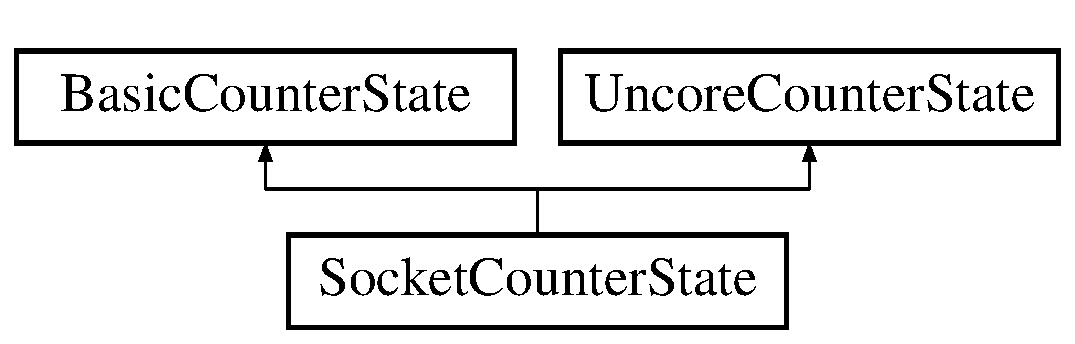
\includegraphics[height=2.000000cm]{class_socket_counter_state}
\end{center}
\end{figure}
\subsection*{Public Member Functions}
\begin{DoxyCompactItemize}
\item 
\mbox{\Hypertarget{class_socket_counter_state_aa23362a4685d2abad8c2c7264bb47eab}\label{class_socket_counter_state_aa23362a4685d2abad8c2c7264bb47eab}} 
void {\bfseries accumulate\+Core\+State} (const \mbox{\hyperlink{class_core_counter_state}{Core\+Counter\+State}} \&o)
\end{DoxyCompactItemize}
\subsection*{Protected Member Functions}
\begin{DoxyCompactItemize}
\item 
\mbox{\Hypertarget{class_socket_counter_state_a43ee7028fd4f9ae929ed5b575e60aadb}\label{class_socket_counter_state_a43ee7028fd4f9ae929ed5b575e60aadb}} 
void {\bfseries read\+And\+Aggregate} (std\+::shared\+\_\+ptr$<$ \mbox{\hyperlink{class_safe_msr_handle}{Safe\+Msr\+Handle}} $>$ handle)
\end{DoxyCompactItemize}
\subsection*{Friends}
\begin{DoxyCompactItemize}
\item 
\mbox{\Hypertarget{class_socket_counter_state_ab5f56d2e95ba3daf52c17b8a1d356d64}\label{class_socket_counter_state_ab5f56d2e95ba3daf52c17b8a1d356d64}} 
class {\bfseries P\+CM}
\end{DoxyCompactItemize}
\subsection*{Additional Inherited Members}


\subsection{Detailed Description}
Socket-\/wide counter state. 

The documentation for this class was generated from the following file\+:\begin{DoxyCompactItemize}
\item 
\mbox{\hyperlink{cpucounters_8h}{cpucounters.\+h}}\end{DoxyCompactItemize}

\hypertarget{class_system_counter_state}{}\section{System\+Counter\+State Class Reference}
\label{class_system_counter_state}\index{System\+Counter\+State@{System\+Counter\+State}}


System-\/wide counter state.  




{\ttfamily \#include $<$cpucounters.\+h$>$}

Inheritance diagram for System\+Counter\+State\+:\begin{figure}[H]
\begin{center}
\leavevmode
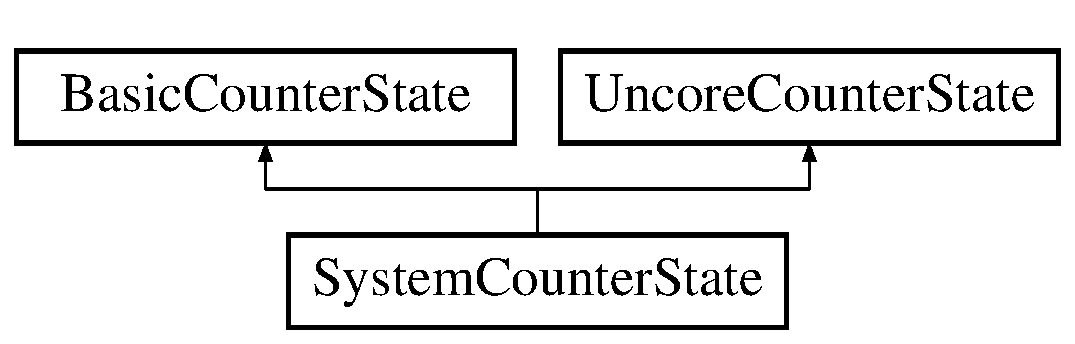
\includegraphics[height=2.000000cm]{class_system_counter_state}
\end{center}
\end{figure}
\subsection*{Public Member Functions}
\begin{DoxyCompactItemize}
\item 
\mbox{\Hypertarget{class_system_counter_state_af8fb0cdf2c4d03ec03b1ef2e4c27aac4}\label{class_system_counter_state_af8fb0cdf2c4d03ec03b1ef2e4c27aac4}} 
void {\bfseries accumulate\+Socket\+State} (const \mbox{\hyperlink{class_socket_counter_state}{Socket\+Counter\+State}} \&o)
\end{DoxyCompactItemize}
\subsection*{Protected Member Functions}
\begin{DoxyCompactItemize}
\item 
\mbox{\Hypertarget{class_system_counter_state_a1755dd4a5ffc57d0423620336aab534b}\label{class_system_counter_state_a1755dd4a5ffc57d0423620336aab534b}} 
void {\bfseries read\+And\+Aggregate} (std\+::shared\+\_\+ptr$<$ \mbox{\hyperlink{class_safe_msr_handle}{Safe\+Msr\+Handle}} $>$ handle)
\end{DoxyCompactItemize}
\subsection*{Friends}
\begin{DoxyCompactItemize}
\item 
\mbox{\Hypertarget{class_system_counter_state_ab5f56d2e95ba3daf52c17b8a1d356d64}\label{class_system_counter_state_ab5f56d2e95ba3daf52c17b8a1d356d64}} 
class {\bfseries P\+CM}
\item 
uint64 \mbox{\hyperlink{class_system_counter_state_aca1b1d8ba1679c4a0c394c2647428fd3}{get\+Incoming\+Q\+P\+I\+Link\+Bytes}} (uint32 socket\+Nr, uint32 link\+Nr, const \mbox{\hyperlink{class_system_counter_state}{System\+Counter\+State}} \&before, const \mbox{\hyperlink{class_system_counter_state}{System\+Counter\+State}} \&after)
\begin{DoxyCompactList}\small\item\em Get estimation of Q\+PI data traffic per incoming Q\+PI link. \end{DoxyCompactList}\item 
uint64 \mbox{\hyperlink{class_system_counter_state_a42d6a119a26ea41c40d5585356d832ca}{get\+Incoming\+Q\+P\+I\+Link\+Bytes}} (uint32 socket\+Nr, uint32 link\+Nr, const \mbox{\hyperlink{class_system_counter_state}{System\+Counter\+State}} \&now)
\begin{DoxyCompactList}\small\item\em Return current value of the counter of Q\+PI data traffic per incoming Q\+PI link. \end{DoxyCompactList}\item 
double \mbox{\hyperlink{class_system_counter_state_ac7b1863133a9a711117fcb8b68d2d773}{get\+Outgoing\+Q\+P\+I\+Link\+Utilization}} (uint32 socket\+Nr, uint32 link\+Nr, const \mbox{\hyperlink{class_system_counter_state}{System\+Counter\+State}} \&before, const \mbox{\hyperlink{class_system_counter_state}{System\+Counter\+State}} \&after)
\begin{DoxyCompactList}\small\item\em Get utilization of outgoing Q\+PI link (0..1) \end{DoxyCompactList}\item 
uint64 \mbox{\hyperlink{class_system_counter_state_a6bdb34d102d7353421bd878da7b9ef23}{get\+Outgoing\+Q\+P\+I\+Link\+Bytes}} (uint32 socket\+Nr, uint32 link\+Nr, const \mbox{\hyperlink{class_system_counter_state}{System\+Counter\+State}} \&before, const \mbox{\hyperlink{class_system_counter_state}{System\+Counter\+State}} \&after)
\begin{DoxyCompactList}\small\item\em Get estimation of Q\+PI (data+nondata) traffic per outgoing Q\+PI link. \end{DoxyCompactList}\item 
\mbox{\Hypertarget{class_system_counter_state_a336f198b4a81e0d34bb581e8bd8be0e0}\label{class_system_counter_state_a336f198b4a81e0d34bb581e8bd8be0e0}} 
uint64 {\bfseries get\+Outgoing\+Q\+P\+I\+Link\+Bytes} (uint32 socket\+Nr, uint32 link\+Nr, const \mbox{\hyperlink{class_system_counter_state}{System\+Counter\+State}} \&now)
\end{DoxyCompactItemize}
\subsection*{Additional Inherited Members}


\subsection{Detailed Description}
System-\/wide counter state. 

\subsection{Friends And Related Function Documentation}
\mbox{\Hypertarget{class_system_counter_state_aca1b1d8ba1679c4a0c394c2647428fd3}\label{class_system_counter_state_aca1b1d8ba1679c4a0c394c2647428fd3}} 
\index{System\+Counter\+State@{System\+Counter\+State}!get\+Incoming\+Q\+P\+I\+Link\+Bytes@{get\+Incoming\+Q\+P\+I\+Link\+Bytes}}
\index{get\+Incoming\+Q\+P\+I\+Link\+Bytes@{get\+Incoming\+Q\+P\+I\+Link\+Bytes}!System\+Counter\+State@{System\+Counter\+State}}
\subsubsection{\texorpdfstring{get\+Incoming\+Q\+P\+I\+Link\+Bytes}{getIncomingQPILinkBytes}\hspace{0.1cm}{\footnotesize\ttfamily [1/2]}}
{\footnotesize\ttfamily uint64 get\+Incoming\+Q\+P\+I\+Link\+Bytes (\begin{DoxyParamCaption}\item[{uint32}]{socket\+Nr,  }\item[{uint32}]{link\+Nr,  }\item[{const \mbox{\hyperlink{class_system_counter_state}{System\+Counter\+State}} \&}]{before,  }\item[{const \mbox{\hyperlink{class_system_counter_state}{System\+Counter\+State}} \&}]{after }\end{DoxyParamCaption})\hspace{0.3cm}{\ttfamily [friend]}}



Get estimation of Q\+PI data traffic per incoming Q\+PI link. 

Returns an estimation of number of data bytes transferred to a socket over Intel(r) Quick Path Interconnect


\begin{DoxyParams}{Parameters}
{\em socket\+Nr} & socket identifier \\
\hline
{\em link\+Nr} & link\+Nr \\
\hline
{\em before} & System C\+PU counter state before the experiment \\
\hline
{\em after} & System C\+PU counter state after the experiment \\
\hline
\end{DoxyParams}
\begin{DoxyReturn}{Returns}
Number of bytes 
\end{DoxyReturn}
\mbox{\Hypertarget{class_system_counter_state_a42d6a119a26ea41c40d5585356d832ca}\label{class_system_counter_state_a42d6a119a26ea41c40d5585356d832ca}} 
\index{System\+Counter\+State@{System\+Counter\+State}!get\+Incoming\+Q\+P\+I\+Link\+Bytes@{get\+Incoming\+Q\+P\+I\+Link\+Bytes}}
\index{get\+Incoming\+Q\+P\+I\+Link\+Bytes@{get\+Incoming\+Q\+P\+I\+Link\+Bytes}!System\+Counter\+State@{System\+Counter\+State}}
\subsubsection{\texorpdfstring{get\+Incoming\+Q\+P\+I\+Link\+Bytes}{getIncomingQPILinkBytes}\hspace{0.1cm}{\footnotesize\ttfamily [2/2]}}
{\footnotesize\ttfamily uint64 get\+Incoming\+Q\+P\+I\+Link\+Bytes (\begin{DoxyParamCaption}\item[{uint32}]{socket\+Nr,  }\item[{uint32}]{link\+Nr,  }\item[{const \mbox{\hyperlink{class_system_counter_state}{System\+Counter\+State}} \&}]{now }\end{DoxyParamCaption})\hspace{0.3cm}{\ttfamily [friend]}}



Return current value of the counter of Q\+PI data traffic per incoming Q\+PI link. 

Returns the number of incoming data bytes to a socket over Intel(r) Quick Path Interconnect


\begin{DoxyParams}{Parameters}
{\em socket\+Nr} & socket identifier \\
\hline
{\em link\+Nr} & link\+Nr \\
\hline
{\em now} & Current System C\+PU counter state \\
\hline
\end{DoxyParams}
\begin{DoxyReturn}{Returns}
Number of bytes 
\end{DoxyReturn}
\mbox{\Hypertarget{class_system_counter_state_a6bdb34d102d7353421bd878da7b9ef23}\label{class_system_counter_state_a6bdb34d102d7353421bd878da7b9ef23}} 
\index{System\+Counter\+State@{System\+Counter\+State}!get\+Outgoing\+Q\+P\+I\+Link\+Bytes@{get\+Outgoing\+Q\+P\+I\+Link\+Bytes}}
\index{get\+Outgoing\+Q\+P\+I\+Link\+Bytes@{get\+Outgoing\+Q\+P\+I\+Link\+Bytes}!System\+Counter\+State@{System\+Counter\+State}}
\subsubsection{\texorpdfstring{get\+Outgoing\+Q\+P\+I\+Link\+Bytes}{getOutgoingQPILinkBytes}}
{\footnotesize\ttfamily uint64 get\+Outgoing\+Q\+P\+I\+Link\+Bytes (\begin{DoxyParamCaption}\item[{uint32}]{socket\+Nr,  }\item[{uint32}]{link\+Nr,  }\item[{const \mbox{\hyperlink{class_system_counter_state}{System\+Counter\+State}} \&}]{before,  }\item[{const \mbox{\hyperlink{class_system_counter_state}{System\+Counter\+State}} \&}]{after }\end{DoxyParamCaption})\hspace{0.3cm}{\ttfamily [friend]}}



Get estimation of Q\+PI (data+nondata) traffic per outgoing Q\+PI link. 

Returns an estimation of number of data bytes transferred from a socket over Intel(r) Quick Path Interconnect


\begin{DoxyParams}{Parameters}
{\em socket\+Nr} & socket identifier \\
\hline
{\em link\+Nr} & link\+Nr \\
\hline
{\em before} & System C\+PU counter state before the experiment \\
\hline
{\em after} & System C\+PU counter state after the experiment \\
\hline
\end{DoxyParams}
\begin{DoxyReturn}{Returns}
Number of bytes 
\end{DoxyReturn}
\mbox{\Hypertarget{class_system_counter_state_ac7b1863133a9a711117fcb8b68d2d773}\label{class_system_counter_state_ac7b1863133a9a711117fcb8b68d2d773}} 
\index{System\+Counter\+State@{System\+Counter\+State}!get\+Outgoing\+Q\+P\+I\+Link\+Utilization@{get\+Outgoing\+Q\+P\+I\+Link\+Utilization}}
\index{get\+Outgoing\+Q\+P\+I\+Link\+Utilization@{get\+Outgoing\+Q\+P\+I\+Link\+Utilization}!System\+Counter\+State@{System\+Counter\+State}}
\subsubsection{\texorpdfstring{get\+Outgoing\+Q\+P\+I\+Link\+Utilization}{getOutgoingQPILinkUtilization}}
{\footnotesize\ttfamily double get\+Outgoing\+Q\+P\+I\+Link\+Utilization (\begin{DoxyParamCaption}\item[{uint32}]{socket\+Nr,  }\item[{uint32}]{link\+Nr,  }\item[{const \mbox{\hyperlink{class_system_counter_state}{System\+Counter\+State}} \&}]{before,  }\item[{const \mbox{\hyperlink{class_system_counter_state}{System\+Counter\+State}} \&}]{after }\end{DoxyParamCaption})\hspace{0.3cm}{\ttfamily [friend]}}



Get utilization of outgoing Q\+PI link (0..1) 

Returns an estimation of utilization of Q\+PI link by (data+nondata) traffic transferred from a socket over Intel(r) Quick Path Interconnect


\begin{DoxyParams}{Parameters}
{\em socket\+Nr} & socket identifier \\
\hline
{\em link\+Nr} & link\+Nr \\
\hline
{\em before} & System C\+PU counter state before the experiment \\
\hline
{\em after} & System C\+PU counter state after the experiment \\
\hline
\end{DoxyParams}
\begin{DoxyReturn}{Returns}
utilization (0..1) 
\end{DoxyReturn}


The documentation for this class was generated from the following file\+:\begin{DoxyCompactItemize}
\item 
\mbox{\hyperlink{cpucounters_8h}{cpucounters.\+h}}\end{DoxyCompactItemize}

\hypertarget{struct_t}{}\section{T Struct Reference}
\label{struct_t}\index{T@{T}}
\subsection*{Public Member Functions}
\begin{DoxyCompactItemize}
\item 
\mbox{\Hypertarget{struct_t_a8f5edc9a39e3241d33ae54a5029b0043}\label{struct_t_a8f5edc9a39e3241d33ae54a5029b0043}} 
{\bfseries T} (int a)
\item 
\mbox{\Hypertarget{struct_t_a548f7076ea10db21bc73979dd9735f47}\label{struct_t_a548f7076ea10db21bc73979dd9735f47}} 
bool {\bfseries operator==} (const \mbox{\hyperlink{struct_t}{T}} \&k) const
\item 
\mbox{\Hypertarget{struct_t_a8f5edc9a39e3241d33ae54a5029b0043}\label{struct_t_a8f5edc9a39e3241d33ae54a5029b0043}} 
{\bfseries T} (int a)
\item 
\mbox{\Hypertarget{struct_t_a548f7076ea10db21bc73979dd9735f47}\label{struct_t_a548f7076ea10db21bc73979dd9735f47}} 
bool {\bfseries operator==} (const \mbox{\hyperlink{struct_t}{T}} \&k) const
\item 
\mbox{\Hypertarget{struct_t_a8f5edc9a39e3241d33ae54a5029b0043}\label{struct_t_a8f5edc9a39e3241d33ae54a5029b0043}} 
{\bfseries T} (int a)
\item 
\mbox{\Hypertarget{struct_t_a548f7076ea10db21bc73979dd9735f47}\label{struct_t_a548f7076ea10db21bc73979dd9735f47}} 
bool {\bfseries operator==} (const \mbox{\hyperlink{struct_t}{T}} \&k) const
\end{DoxyCompactItemize}
\subsection*{Public Attributes}
\begin{DoxyCompactItemize}
\item 
\mbox{\Hypertarget{struct_t_a910785bad87bed60eccfe8fec17e55ec}\label{struct_t_a910785bad87bed60eccfe8fec17e55ec}} 
int {\bfseries key} \mbox{[}1\mbox{]}
\item 
\mbox{\Hypertarget{struct_t_a07547b3bcc7ade309011aaa5a56ec814}\label{struct_t_a07547b3bcc7ade309011aaa5a56ec814}} 
int {\bfseries data} \mbox{[}3\mbox{]}
\end{DoxyCompactItemize}


The documentation for this struct was generated from the following files\+:\begin{DoxyCompactItemize}
\item 
memoptest.\+cpp\item 
readmem.\+cpp\item 
\mbox{\hyperlink{realtime_8cpp}{realtime.\+cpp}}\end{DoxyCompactItemize}

\hypertarget{class_temporal_thread_affinity}{}\section{Temporal\+Thread\+Affinity Class Reference}
\label{class_temporal_thread_affinity}\index{Temporal\+Thread\+Affinity@{Temporal\+Thread\+Affinity}}
\subsection*{Public Member Functions}
\begin{DoxyCompactItemize}
\item 
\mbox{\Hypertarget{class_temporal_thread_affinity_adc237efcc45938f0c188e705b2ed226e}\label{class_temporal_thread_affinity_adc237efcc45938f0c188e705b2ed226e}} 
{\bfseries Temporal\+Thread\+Affinity} (uint32)
\item 
\mbox{\Hypertarget{class_temporal_thread_affinity_aae90a72724e0fbb83b3e9607679d27ca}\label{class_temporal_thread_affinity_aae90a72724e0fbb83b3e9607679d27ca}} 
bool {\bfseries supported} () const
\end{DoxyCompactItemize}


The documentation for this class was generated from the following file\+:\begin{DoxyCompactItemize}
\item 
\mbox{\hyperlink{cpucounters_8cpp}{cpucounters.\+cpp}}\end{DoxyCompactItemize}

\hypertarget{struct_topology_entry}{}\section{Topology\+Entry Struct Reference}
\label{struct_topology_entry}\index{Topology\+Entry@{Topology\+Entry}}
\subsection*{Public Attributes}
\begin{DoxyCompactItemize}
\item 
\mbox{\Hypertarget{struct_topology_entry_aa960a8bbdd754740d781072ae1266eed}\label{struct_topology_entry_aa960a8bbdd754740d781072ae1266eed}} 
int32 {\bfseries os\+\_\+id}
\item 
\mbox{\Hypertarget{struct_topology_entry_a1db41da84b81248561c0c0b00739939f}\label{struct_topology_entry_a1db41da84b81248561c0c0b00739939f}} 
int32 {\bfseries thread\+\_\+id}
\item 
\mbox{\Hypertarget{struct_topology_entry_aee7bef9e2b54f9617a697a43068a5c27}\label{struct_topology_entry_aee7bef9e2b54f9617a697a43068a5c27}} 
int32 {\bfseries core\+\_\+id}
\item 
\mbox{\Hypertarget{struct_topology_entry_a620e9508cdcd78b979ffaabe2581afd1}\label{struct_topology_entry_a620e9508cdcd78b979ffaabe2581afd1}} 
int32 {\bfseries tile\+\_\+id}
\item 
\mbox{\Hypertarget{struct_topology_entry_a9b217468c64b3072b48ad5466742827e}\label{struct_topology_entry_a9b217468c64b3072b48ad5466742827e}} 
int32 {\bfseries socket}
\end{DoxyCompactItemize}


The documentation for this struct was generated from the following file\+:\begin{DoxyCompactItemize}
\item 
\mbox{\hyperlink{cpucounters_8h}{cpucounters.\+h}}\end{DoxyCompactItemize}

\hypertarget{struct_t_s_x_event}{}\section{T\+S\+X\+Event Struct Reference}
\label{struct_t_s_x_event}\index{T\+S\+X\+Event@{T\+S\+X\+Event}}
\subsection*{Public Attributes}
\begin{DoxyCompactItemize}
\item 
\mbox{\Hypertarget{struct_t_s_x_event_a592441448f28d73655c864f5dbb77538}\label{struct_t_s_x_event_a592441448f28d73655c864f5dbb77538}} 
const char $\ast$ {\bfseries name}
\item 
\mbox{\Hypertarget{struct_t_s_x_event_a45969e694e699c485379594701bd7e35}\label{struct_t_s_x_event_a45969e694e699c485379594701bd7e35}} 
unsigned char {\bfseries event}
\item 
\mbox{\Hypertarget{struct_t_s_x_event_a2f1b2f588a4641abde0dd5bd7870a537}\label{struct_t_s_x_event_a2f1b2f588a4641abde0dd5bd7870a537}} 
unsigned char {\bfseries umask}
\item 
\mbox{\Hypertarget{struct_t_s_x_event_aae0d6de90f1596c51b6c0345356a1076}\label{struct_t_s_x_event_aae0d6de90f1596c51b6c0345356a1076}} 
const char $\ast$ {\bfseries description}
\end{DoxyCompactItemize}


The documentation for this struct was generated from the following file\+:\begin{DoxyCompactItemize}
\item 
\mbox{\hyperlink{pcm-tsx_8cpp}{pcm-\/tsx.\+cpp}}\end{DoxyCompactItemize}

\hypertarget{class_uncore_counter_state}{}\section{Uncore\+Counter\+State Class Reference}
\label{class_uncore_counter_state}\index{Uncore\+Counter\+State@{Uncore\+Counter\+State}}


Basic uncore counter state.  




{\ttfamily \#include $<$cpucounters.\+h$>$}

Inheritance diagram for Uncore\+Counter\+State\+:\begin{figure}[H]
\begin{center}
\leavevmode
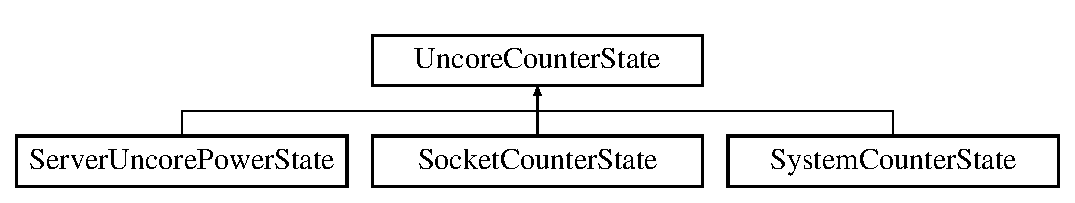
\includegraphics[height=2.000000cm]{class_uncore_counter_state}
\end{center}
\end{figure}
\subsection*{Public Member Functions}
\begin{DoxyCompactItemize}
\item 
\mbox{\Hypertarget{class_uncore_counter_state_a96eb270d92f202a85ed11ded8cf60f71}\label{class_uncore_counter_state_a96eb270d92f202a85ed11ded8cf60f71}} 
\mbox{\hyperlink{class_uncore_counter_state}{Uncore\+Counter\+State}} \& {\bfseries operator+=} (const \mbox{\hyperlink{class_uncore_counter_state}{Uncore\+Counter\+State}} \&o)
\end{DoxyCompactItemize}
\subsection*{Protected Member Functions}
\begin{DoxyCompactItemize}
\item 
\mbox{\Hypertarget{class_uncore_counter_state_a2583a9807bb67e008e6ffde1cd13850f}\label{class_uncore_counter_state_a2583a9807bb67e008e6ffde1cd13850f}} 
void {\bfseries read\+And\+Aggregate} (std\+::shared\+\_\+ptr$<$ \mbox{\hyperlink{class_safe_msr_handle}{Safe\+Msr\+Handle}} $>$)
\end{DoxyCompactItemize}
\subsection*{Protected Attributes}
\begin{DoxyCompactItemize}
\item 
\mbox{\Hypertarget{class_uncore_counter_state_a3e59bb4c79f6040b17b104194a5e29fb}\label{class_uncore_counter_state_a3e59bb4c79f6040b17b104194a5e29fb}} 
uint64 {\bfseries Unc\+M\+C\+Full\+Writes}
\item 
\mbox{\Hypertarget{class_uncore_counter_state_a5a07c23a907365682137c5d8c1cf79ad}\label{class_uncore_counter_state_a5a07c23a907365682137c5d8c1cf79ad}} 
uint64 {\bfseries Unc\+M\+C\+Normal\+Reads}
\item 
\mbox{\Hypertarget{class_uncore_counter_state_a933afbcf1236a619c7459e84b55b0528}\label{class_uncore_counter_state_a933afbcf1236a619c7459e84b55b0528}} 
uint64 {\bfseries Unc\+E\+D\+C\+Full\+Writes}
\item 
\mbox{\Hypertarget{class_uncore_counter_state_ac5a6269e7564fd952331a78e2cb47adb}\label{class_uncore_counter_state_ac5a6269e7564fd952331a78e2cb47adb}} 
uint64 {\bfseries Unc\+E\+D\+C\+Normal\+Reads}
\item 
\mbox{\Hypertarget{class_uncore_counter_state_a4c3d0db74283d9420d9089e2c2553561}\label{class_uncore_counter_state_a4c3d0db74283d9420d9089e2c2553561}} 
uint64 {\bfseries Unc\+M\+C\+I\+O\+Requests}
\item 
\mbox{\Hypertarget{class_uncore_counter_state_a74bdee47e68bbc55c2ee023fc3bfe76d}\label{class_uncore_counter_state_a74bdee47e68bbc55c2ee023fc3bfe76d}} 
uint64 {\bfseries Package\+Energy\+Status}
\item 
\mbox{\Hypertarget{class_uncore_counter_state_a03c78bbb9fb36c84c075b8d72fc5eed9}\label{class_uncore_counter_state_a03c78bbb9fb36c84c075b8d72fc5eed9}} 
uint64 {\bfseries D\+R\+A\+M\+Energy\+Status}
\item 
\mbox{\Hypertarget{class_uncore_counter_state_ad9c072ee0fdc984b82d0c143a186ce37}\label{class_uncore_counter_state_ad9c072ee0fdc984b82d0c143a186ce37}} 
uint64 {\bfseries T\+O\+R\+Occupancy\+I\+A\+Miss}
\item 
\mbox{\Hypertarget{class_uncore_counter_state_a92b8e5a10e1b634824a6a17049a777bd}\label{class_uncore_counter_state_a92b8e5a10e1b634824a6a17049a777bd}} 
uint64 {\bfseries T\+O\+R\+Inserts\+I\+A\+Miss}
\item 
\mbox{\Hypertarget{class_uncore_counter_state_a515a8614f806f057d4a092a9f4a5c473}\label{class_uncore_counter_state_a515a8614f806f057d4a092a9f4a5c473}} 
uint64 {\bfseries Unc\+Clocks}
\item 
\mbox{\Hypertarget{class_uncore_counter_state_a5819f82036b4386ca638d0755cdc7388}\label{class_uncore_counter_state_a5819f82036b4386ca638d0755cdc7388}} 
uint64 {\bfseries C\+State\+Residency} \mbox{[}P\+C\+M\+::\+M\+A\+X\+\_\+\+C\+\_\+\+S\+T\+A\+TE+1\mbox{]}
\end{DoxyCompactItemize}
\subsection*{Friends}
\begin{DoxyCompactItemize}
\item 
\mbox{\Hypertarget{class_uncore_counter_state_ab5f56d2e95ba3daf52c17b8a1d356d64}\label{class_uncore_counter_state_ab5f56d2e95ba3daf52c17b8a1d356d64}} 
class {\bfseries P\+CM}
\item 
{\footnotesize template$<$class Counter\+State\+Type $>$ }\\uint64 \mbox{\hyperlink{class_uncore_counter_state_a0f28a32a3edeaecd916ba097aee99d7f}{get\+Bytes\+Read\+From\+MC}} (const Counter\+State\+Type \&before, const Counter\+State\+Type \&after)
\begin{DoxyCompactList}\small\item\em Computes number of bytes read from D\+R\+AM memory controllers. \end{DoxyCompactList}\item 
{\footnotesize template$<$class Counter\+State\+Type $>$ }\\uint64 \mbox{\hyperlink{class_uncore_counter_state_a24fce7df2ee7140db18ecfcd74fe63d1}{get\+Bytes\+Written\+To\+MC}} (const Counter\+State\+Type \&before, const Counter\+State\+Type \&after)
\begin{DoxyCompactList}\small\item\em Computes number of bytes written to D\+R\+AM memory controllers. \end{DoxyCompactList}\item 
{\footnotesize template$<$class Counter\+State\+Type $>$ }\\uint64 \mbox{\hyperlink{class_uncore_counter_state_a8a7e839f24a02691d4b3509fc2adee51}{get\+Bytes\+Read\+From\+E\+DC}} (const Counter\+State\+Type \&before, const Counter\+State\+Type \&after)
\begin{DoxyCompactList}\small\item\em Computes number of bytes read from M\+C\+D\+R\+AM memory controllers. \end{DoxyCompactList}\item 
{\footnotesize template$<$class Counter\+State\+Type $>$ }\\uint64 \mbox{\hyperlink{class_uncore_counter_state_aface6421f7c3e654bcf411abd7cea990}{get\+Bytes\+Written\+To\+E\+DC}} (const Counter\+State\+Type \&before, const Counter\+State\+Type \&after)
\begin{DoxyCompactList}\small\item\em Computes number of bytes written to M\+C\+D\+R\+AM memory controllers. \end{DoxyCompactList}\item 
{\footnotesize template$<$class Counter\+State\+Type $>$ }\\uint64 \mbox{\hyperlink{class_uncore_counter_state_a7e5434dba3a810501f289329e52b889d}{get\+I\+O\+Request\+Bytes\+From\+MC}} (const Counter\+State\+Type \&before, const Counter\+State\+Type \&after)
\begin{DoxyCompactList}\small\item\em Computes number of bytes of read/write requests from all IO sources. \end{DoxyCompactList}\item 
{\footnotesize template$<$class Counter\+State\+Type $>$ }\\uint64 \mbox{\hyperlink{class_uncore_counter_state_a054b949f09283093e1923affa4e58ae8}{get\+Consumed\+Energy}} (const Counter\+State\+Type \&before, const Counter\+State\+Type \&after)
\begin{DoxyCompactList}\small\item\em Returns energy consumed by processor, exclusing D\+R\+AM (measured in internal units) \end{DoxyCompactList}\item 
{\footnotesize template$<$class Counter\+State\+Type $>$ }\\uint64 \mbox{\hyperlink{class_uncore_counter_state_a71af0766460ef7dd3d138ec0d0924eda}{get\+D\+R\+A\+M\+Consumed\+Energy}} (const Counter\+State\+Type \&before, const Counter\+State\+Type \&after)
\begin{DoxyCompactList}\small\item\em Returns energy consumed by D\+R\+AM (measured in internal units) \end{DoxyCompactList}\item 
{\footnotesize template$<$class Counter\+State\+Type $>$ }\\double \mbox{\hyperlink{class_uncore_counter_state_a5e34f7b0326dda86b54fcb7bb84a0b38}{get\+Package\+C\+State\+Residency}} (int state, const Counter\+State\+Type \&before, const Counter\+State\+Type \&after)
\begin{DoxyCompactList}\small\item\em Computes residency in the package C-\/state. \end{DoxyCompactList}\item 
\mbox{\Hypertarget{class_uncore_counter_state_a6791e3fe842320171cbac393e55929f6}\label{class_uncore_counter_state_a6791e3fe842320171cbac393e55929f6}} 
{\footnotesize template$<$class Counter\+State\+Type $>$ }\\double \mbox{\hyperlink{class_uncore_counter_state_a6791e3fe842320171cbac393e55929f6}{get\+L\+L\+C\+Read\+Miss\+Latency}} (const Counter\+State\+Type \&before, const Counter\+State\+Type \&after)
\begin{DoxyCompactList}\small\item\em Returns average last level cache read+prefetch miss latency in ns. \end{DoxyCompactList}\end{DoxyCompactItemize}


\subsection{Detailed Description}
Basic uncore counter state. 

Intended only for derivation, but not for the direct use 

\subsection{Friends And Related Function Documentation}
\mbox{\Hypertarget{class_uncore_counter_state_a8a7e839f24a02691d4b3509fc2adee51}\label{class_uncore_counter_state_a8a7e839f24a02691d4b3509fc2adee51}} 
\index{Uncore\+Counter\+State@{Uncore\+Counter\+State}!get\+Bytes\+Read\+From\+E\+DC@{get\+Bytes\+Read\+From\+E\+DC}}
\index{get\+Bytes\+Read\+From\+E\+DC@{get\+Bytes\+Read\+From\+E\+DC}!Uncore\+Counter\+State@{Uncore\+Counter\+State}}
\subsubsection{\texorpdfstring{get\+Bytes\+Read\+From\+E\+DC}{getBytesReadFromEDC}}
{\footnotesize\ttfamily template$<$class Counter\+State\+Type $>$ \\
uint64 get\+Bytes\+Read\+From\+E\+DC (\begin{DoxyParamCaption}\item[{const Counter\+State\+Type \&}]{before,  }\item[{const Counter\+State\+Type \&}]{after }\end{DoxyParamCaption})\hspace{0.3cm}{\ttfamily [friend]}}



Computes number of bytes read from M\+C\+D\+R\+AM memory controllers. 


\begin{DoxyParams}{Parameters}
{\em before} & C\+PU counter state before the experiment \\
\hline
{\em after} & C\+PU counter state after the experiment \\
\hline
\end{DoxyParams}
\begin{DoxyReturn}{Returns}
Number of bytes 
\end{DoxyReturn}
\mbox{\Hypertarget{class_uncore_counter_state_a0f28a32a3edeaecd916ba097aee99d7f}\label{class_uncore_counter_state_a0f28a32a3edeaecd916ba097aee99d7f}} 
\index{Uncore\+Counter\+State@{Uncore\+Counter\+State}!get\+Bytes\+Read\+From\+MC@{get\+Bytes\+Read\+From\+MC}}
\index{get\+Bytes\+Read\+From\+MC@{get\+Bytes\+Read\+From\+MC}!Uncore\+Counter\+State@{Uncore\+Counter\+State}}
\subsubsection{\texorpdfstring{get\+Bytes\+Read\+From\+MC}{getBytesReadFromMC}}
{\footnotesize\ttfamily template$<$class Counter\+State\+Type $>$ \\
uint64 get\+Bytes\+Read\+From\+MC (\begin{DoxyParamCaption}\item[{const Counter\+State\+Type \&}]{before,  }\item[{const Counter\+State\+Type \&}]{after }\end{DoxyParamCaption})\hspace{0.3cm}{\ttfamily [friend]}}



Computes number of bytes read from D\+R\+AM memory controllers. 


\begin{DoxyParams}{Parameters}
{\em before} & C\+PU counter state before the experiment \\
\hline
{\em after} & C\+PU counter state after the experiment \\
\hline
\end{DoxyParams}
\begin{DoxyReturn}{Returns}
Number of bytes 
\end{DoxyReturn}
\mbox{\Hypertarget{class_uncore_counter_state_aface6421f7c3e654bcf411abd7cea990}\label{class_uncore_counter_state_aface6421f7c3e654bcf411abd7cea990}} 
\index{Uncore\+Counter\+State@{Uncore\+Counter\+State}!get\+Bytes\+Written\+To\+E\+DC@{get\+Bytes\+Written\+To\+E\+DC}}
\index{get\+Bytes\+Written\+To\+E\+DC@{get\+Bytes\+Written\+To\+E\+DC}!Uncore\+Counter\+State@{Uncore\+Counter\+State}}
\subsubsection{\texorpdfstring{get\+Bytes\+Written\+To\+E\+DC}{getBytesWrittenToEDC}}
{\footnotesize\ttfamily template$<$class Counter\+State\+Type $>$ \\
uint64 get\+Bytes\+Written\+To\+E\+DC (\begin{DoxyParamCaption}\item[{const Counter\+State\+Type \&}]{before,  }\item[{const Counter\+State\+Type \&}]{after }\end{DoxyParamCaption})\hspace{0.3cm}{\ttfamily [friend]}}



Computes number of bytes written to M\+C\+D\+R\+AM memory controllers. 


\begin{DoxyParams}{Parameters}
{\em before} & C\+PU counter state before the experiment \\
\hline
{\em after} & C\+PU counter state after the experiment \\
\hline
\end{DoxyParams}
\begin{DoxyReturn}{Returns}
Number of bytes 
\end{DoxyReturn}
\mbox{\Hypertarget{class_uncore_counter_state_a24fce7df2ee7140db18ecfcd74fe63d1}\label{class_uncore_counter_state_a24fce7df2ee7140db18ecfcd74fe63d1}} 
\index{Uncore\+Counter\+State@{Uncore\+Counter\+State}!get\+Bytes\+Written\+To\+MC@{get\+Bytes\+Written\+To\+MC}}
\index{get\+Bytes\+Written\+To\+MC@{get\+Bytes\+Written\+To\+MC}!Uncore\+Counter\+State@{Uncore\+Counter\+State}}
\subsubsection{\texorpdfstring{get\+Bytes\+Written\+To\+MC}{getBytesWrittenToMC}}
{\footnotesize\ttfamily template$<$class Counter\+State\+Type $>$ \\
uint64 get\+Bytes\+Written\+To\+MC (\begin{DoxyParamCaption}\item[{const Counter\+State\+Type \&}]{before,  }\item[{const Counter\+State\+Type \&}]{after }\end{DoxyParamCaption})\hspace{0.3cm}{\ttfamily [friend]}}



Computes number of bytes written to D\+R\+AM memory controllers. 


\begin{DoxyParams}{Parameters}
{\em before} & C\+PU counter state before the experiment \\
\hline
{\em after} & C\+PU counter state after the experiment \\
\hline
\end{DoxyParams}
\begin{DoxyReturn}{Returns}
Number of bytes 
\end{DoxyReturn}
\mbox{\Hypertarget{class_uncore_counter_state_a054b949f09283093e1923affa4e58ae8}\label{class_uncore_counter_state_a054b949f09283093e1923affa4e58ae8}} 
\index{Uncore\+Counter\+State@{Uncore\+Counter\+State}!get\+Consumed\+Energy@{get\+Consumed\+Energy}}
\index{get\+Consumed\+Energy@{get\+Consumed\+Energy}!Uncore\+Counter\+State@{Uncore\+Counter\+State}}
\subsubsection{\texorpdfstring{get\+Consumed\+Energy}{getConsumedEnergy}}
{\footnotesize\ttfamily template$<$class Counter\+State\+Type $>$ \\
uint64 get\+Consumed\+Energy (\begin{DoxyParamCaption}\item[{const Counter\+State\+Type \&}]{before,  }\item[{const Counter\+State\+Type \&}]{after }\end{DoxyParamCaption})\hspace{0.3cm}{\ttfamily [friend]}}



Returns energy consumed by processor, exclusing D\+R\+AM (measured in internal units) 


\begin{DoxyParams}{Parameters}
{\em before} & C\+PU counter state before the experiment \\
\hline
{\em after} & C\+PU counter state after the experiment \\
\hline
\end{DoxyParams}
\mbox{\Hypertarget{class_uncore_counter_state_a71af0766460ef7dd3d138ec0d0924eda}\label{class_uncore_counter_state_a71af0766460ef7dd3d138ec0d0924eda}} 
\index{Uncore\+Counter\+State@{Uncore\+Counter\+State}!get\+D\+R\+A\+M\+Consumed\+Energy@{get\+D\+R\+A\+M\+Consumed\+Energy}}
\index{get\+D\+R\+A\+M\+Consumed\+Energy@{get\+D\+R\+A\+M\+Consumed\+Energy}!Uncore\+Counter\+State@{Uncore\+Counter\+State}}
\subsubsection{\texorpdfstring{get\+D\+R\+A\+M\+Consumed\+Energy}{getDRAMConsumedEnergy}}
{\footnotesize\ttfamily template$<$class Counter\+State\+Type $>$ \\
uint64 get\+D\+R\+A\+M\+Consumed\+Energy (\begin{DoxyParamCaption}\item[{const Counter\+State\+Type \&}]{before,  }\item[{const Counter\+State\+Type \&}]{after }\end{DoxyParamCaption})\hspace{0.3cm}{\ttfamily [friend]}}



Returns energy consumed by D\+R\+AM (measured in internal units) 


\begin{DoxyParams}{Parameters}
{\em before} & C\+PU counter state before the experiment \\
\hline
{\em after} & C\+PU counter state after the experiment \\
\hline
\end{DoxyParams}
\mbox{\Hypertarget{class_uncore_counter_state_a7e5434dba3a810501f289329e52b889d}\label{class_uncore_counter_state_a7e5434dba3a810501f289329e52b889d}} 
\index{Uncore\+Counter\+State@{Uncore\+Counter\+State}!get\+I\+O\+Request\+Bytes\+From\+MC@{get\+I\+O\+Request\+Bytes\+From\+MC}}
\index{get\+I\+O\+Request\+Bytes\+From\+MC@{get\+I\+O\+Request\+Bytes\+From\+MC}!Uncore\+Counter\+State@{Uncore\+Counter\+State}}
\subsubsection{\texorpdfstring{get\+I\+O\+Request\+Bytes\+From\+MC}{getIORequestBytesFromMC}}
{\footnotesize\ttfamily template$<$class Counter\+State\+Type $>$ \\
uint64 get\+I\+O\+Request\+Bytes\+From\+MC (\begin{DoxyParamCaption}\item[{const Counter\+State\+Type \&}]{before,  }\item[{const Counter\+State\+Type \&}]{after }\end{DoxyParamCaption})\hspace{0.3cm}{\ttfamily [friend]}}



Computes number of bytes of read/write requests from all IO sources. 


\begin{DoxyParams}{Parameters}
{\em before} & C\+PU counter state before the experiment \\
\hline
{\em after} & C\+PU counter state after the experiment \\
\hline
\end{DoxyParams}
\begin{DoxyReturn}{Returns}
Number of bytes 
\end{DoxyReturn}
\mbox{\Hypertarget{class_uncore_counter_state_a5e34f7b0326dda86b54fcb7bb84a0b38}\label{class_uncore_counter_state_a5e34f7b0326dda86b54fcb7bb84a0b38}} 
\index{Uncore\+Counter\+State@{Uncore\+Counter\+State}!get\+Package\+C\+State\+Residency@{get\+Package\+C\+State\+Residency}}
\index{get\+Package\+C\+State\+Residency@{get\+Package\+C\+State\+Residency}!Uncore\+Counter\+State@{Uncore\+Counter\+State}}
\subsubsection{\texorpdfstring{get\+Package\+C\+State\+Residency}{getPackageCStateResidency}}
{\footnotesize\ttfamily template$<$class Counter\+State\+Type $>$ \\
double get\+Package\+C\+State\+Residency (\begin{DoxyParamCaption}\item[{int}]{state,  }\item[{const Counter\+State\+Type \&}]{before,  }\item[{const Counter\+State\+Type \&}]{after }\end{DoxyParamCaption})\hspace{0.3cm}{\ttfamily [friend]}}



Computes residency in the package C-\/state. 


\begin{DoxyParams}{Parameters}
{\em state} & C-\/state \\
\hline
{\em before} & C\+PU counter state before the experiment \\
\hline
{\em after} & C\+PU counter state after the experiment \\
\hline
\end{DoxyParams}
\begin{DoxyReturn}{Returns}
residence ratio (0..1)\+: 0 -\/ 0\%, 1.\+0 -\/ 100\% 
\end{DoxyReturn}


The documentation for this class was generated from the following files\+:\begin{DoxyCompactItemize}
\item 
\mbox{\hyperlink{cpucounters_8h}{cpucounters.\+h}}\item 
\mbox{\hyperlink{cpucounters_8cpp}{cpucounters.\+cpp}}\end{DoxyCompactItemize}

\hypertarget{struct_uncore_event_select_register}{}\section{Uncore\+Event\+Select\+Register Struct Reference}
\label{struct_uncore_event_select_register}\index{Uncore\+Event\+Select\+Register@{Uncore\+Event\+Select\+Register}}
\subsection*{Public Attributes}
\begin{DoxyCompactItemize}
\item 
\mbox{\Hypertarget{struct_uncore_event_select_register_a781df49c14f3b13df85e8cb9190a0394}\label{struct_uncore_event_select_register_a781df49c14f3b13df85e8cb9190a0394}} 
\begin{tabbing}
xx\=xx\=xx\=xx\=xx\=xx\=xx\=xx\=xx\=\kill
union \{\\
\>struct \{\\
\>\>uint64 {\bfseries event\_select}: 8\\
\>\>uint64 {\bfseries umask}: 8\\
\>\>uint64 {\bfseries reserved1}: 1\\
\>\>uint64 {\bfseries occ\_ctr\_rst}: 1\\
\>\>uint64 {\bfseries edge}: 1\\
\>\>uint64 {\bfseries reserved2}: 1\\
\>\>uint64 {\bfseries enable\_pmi}: 1\\
\>\>uint64 {\bfseries reserved3}: 1\\
\>\>uint64 {\bfseries enable}: 1\\
\>\>uint64 {\bfseries invert}: 1\\
\>\>uint64 {\bfseries cmask}: 8\\
\>\>uint64 {\bfseries reservedx}: 32\\
\>\} {\bfseries fields}\\
\>uint64 {\bfseries value}\\
\}; \\

\end{tabbing}\end{DoxyCompactItemize}


The documentation for this struct was generated from the following file\+:\begin{DoxyCompactItemize}
\item 
\mbox{\hyperlink{types_8h}{types.\+h}}\end{DoxyCompactItemize}

\chapter{File Documentation}
\hypertarget{client__bw_8h}{}\section{client\+\_\+bw.\+h File Reference}
\label{client__bw_8h}\index{client\+\_\+bw.\+h@{client\+\_\+bw.\+h}}


Interface to access client bandwidth counters.  


{\ttfamily \#include \char`\"{}types.\+h\char`\"{}}\newline
{\ttfamily \#include $<$unistd.\+h$>$}\newline
{\ttfamily \#include \char`\"{}mutex.\+h\char`\"{}}\newline
{\ttfamily \#include $<$memory$>$}\newline
\subsection*{Classes}
\begin{DoxyCompactItemize}
\item 
class \mbox{\hyperlink{class_client_b_w}{Client\+BW}}
\end{DoxyCompactItemize}
\subsection*{Macros}
\begin{DoxyCompactItemize}
\item 
\mbox{\Hypertarget{client__bw_8h_aa16cd48b0adede371be77dbc0be2fd9b}\label{client__bw_8h_aa16cd48b0adede371be77dbc0be2fd9b}} 
\#define {\bfseries P\+C\+M\+\_\+\+C\+L\+I\+E\+N\+T\+\_\+\+I\+M\+C\+\_\+\+B\+A\+R\+\_\+\+O\+F\+F\+S\+ET}~(0x0048)
\item 
\mbox{\Hypertarget{client__bw_8h_a2afb60758e870c73eec7e100b6040b47}\label{client__bw_8h_a2afb60758e870c73eec7e100b6040b47}} 
\#define {\bfseries P\+C\+M\+\_\+\+C\+L\+I\+E\+N\+T\+\_\+\+I\+M\+C\+\_\+\+D\+R\+A\+M\+\_\+\+I\+O\+\_\+\+R\+E\+Q\+E\+S\+TS}~(0x5048)
\item 
\mbox{\Hypertarget{client__bw_8h_a125dc536cbcf631a395c40a183645e89}\label{client__bw_8h_a125dc536cbcf631a395c40a183645e89}} 
\#define {\bfseries P\+C\+M\+\_\+\+C\+L\+I\+E\+N\+T\+\_\+\+I\+M\+C\+\_\+\+D\+R\+A\+M\+\_\+\+D\+A\+T\+A\+\_\+\+R\+E\+A\+DS}~(0x5050)
\item 
\mbox{\Hypertarget{client__bw_8h_aca3e4d8c51b41ea7c8465d3f89659796}\label{client__bw_8h_aca3e4d8c51b41ea7c8465d3f89659796}} 
\#define {\bfseries P\+C\+M\+\_\+\+C\+L\+I\+E\+N\+T\+\_\+\+I\+M\+C\+\_\+\+D\+R\+A\+M\+\_\+\+D\+A\+T\+A\+\_\+\+W\+R\+I\+T\+ES}~(0x5054)
\item 
\mbox{\Hypertarget{client__bw_8h_aa0e78fbc5472bbfb796c575dd9c33dba}\label{client__bw_8h_aa0e78fbc5472bbfb796c575dd9c33dba}} 
\#define {\bfseries P\+C\+M\+\_\+\+C\+L\+I\+E\+N\+T\+\_\+\+I\+M\+C\+\_\+\+M\+M\+A\+P\+\_\+\+S\+I\+ZE}~(0x6000)
\end{DoxyCompactItemize}


\subsection{Detailed Description}
Interface to access client bandwidth counters. 


\hypertarget{cpuasynchcounter_8h}{}\section{cpuasynchcounter.\+h File Reference}
\label{cpuasynchcounter_8h}\index{cpuasynchcounter.\+h@{cpuasynchcounter.\+h}}


Implementation of a P\+O\+S\+IX thread that periodically saves the current state of counters and exposes them to other threads.  


{\ttfamily \#include $<$pthread.\+h$>$}\newline
{\ttfamily \#include $<$stdlib.\+h$>$}\newline
{\ttfamily \#include \char`\"{}cpucounters.\+h\char`\"{}}\newline
\subsection*{Classes}
\begin{DoxyCompactItemize}
\item 
class \mbox{\hyperlink{class_asynchron_counter_state}{Asynchron\+Counter\+State}}
\end{DoxyCompactItemize}
\subsection*{Macros}
\begin{DoxyCompactItemize}
\item 
\mbox{\Hypertarget{cpuasynchcounter_8h_a62249e384b997229a3e2ae74ade334e2}\label{cpuasynchcounter_8h_a62249e384b997229a3e2ae74ade334e2}} 
\#define {\bfseries D\+E\+L\+AY}~1
\end{DoxyCompactItemize}
\subsection*{Functions}
\begin{DoxyCompactItemize}
\item 
\mbox{\Hypertarget{cpuasynchcounter_8h_adfa97f5f86f053c95e1c725b790a3922}\label{cpuasynchcounter_8h_adfa97f5f86f053c95e1c725b790a3922}} 
void $\ast$ {\bfseries Update\+Counters} (void $\ast$)
\end{DoxyCompactItemize}


\subsection{Detailed Description}
Implementation of a P\+O\+S\+IX thread that periodically saves the current state of counters and exposes them to other threads. 


\hypertarget{cpucounters_8cpp}{}\section{cpucounters.\+cpp File Reference}
\label{cpucounters_8cpp}\index{cpucounters.\+cpp@{cpucounters.\+cpp}}


The bulk of \mbox{\hyperlink{class_p_c_m}{P\+CM}} implementation.  


{\ttfamily \#include $<$stdio.\+h$>$}\newline
{\ttfamily \#include $<$assert.\+h$>$}\newline
{\ttfamily \#include \char`\"{}cpucounters.\+h\char`\"{}}\newline
{\ttfamily \#include \char`\"{}msr.\+h\char`\"{}}\newline
{\ttfamily \#include \char`\"{}pci.\+h\char`\"{}}\newline
{\ttfamily \#include \char`\"{}types.\+h\char`\"{}}\newline
{\ttfamily \#include \char`\"{}utils.\+h\char`\"{}}\newline
{\ttfamily \#include $<$pthread.\+h$>$}\newline
{\ttfamily \#include $<$errno.\+h$>$}\newline
{\ttfamily \#include $<$sys/time.\+h$>$}\newline
{\ttfamily \#include $<$string.\+h$>$}\newline
{\ttfamily \#include $<$limits$>$}\newline
{\ttfamily \#include $<$map$>$}\newline
{\ttfamily \#include $<$algorithm$>$}\newline
{\ttfamily \#include $<$thread$>$}\newline
{\ttfamily \#include $<$future$>$}\newline
{\ttfamily \#include $<$functional$>$}\newline
{\ttfamily \#include $<$queue$>$}\newline
{\ttfamily \#include $<$condition\+\_\+variable$>$}\newline
{\ttfamily \#include $<$mutex$>$}\newline
{\ttfamily \#include $<$atomic$>$}\newline
\subsection*{Classes}
\begin{DoxyCompactItemize}
\item 
class \mbox{\hyperlink{class_instance_lock}{Instance\+Lock}}
\item 
class \mbox{\hyperlink{class_temporal_thread_affinity}{Temporal\+Thread\+Affinity}}
\item 
union \mbox{\hyperlink{union_p_c_m___c_p_u_i_d___i_n_f_o}{P\+C\+M\+\_\+\+C\+P\+U\+I\+D\+\_\+\+I\+N\+FO}}
\item 
class \mbox{\hyperlink{class_core_task_queue}{Core\+Task\+Queue}}
\end{DoxyCompactItemize}
\subsection*{Macros}
\begin{DoxyCompactItemize}
\item 
\mbox{\Hypertarget{cpucounters_8cpp_a688a679ca6c13e1a60f7f8b70f496f31}\label{cpucounters_8cpp_a688a679ca6c13e1a60f7f8b70f496f31}} 
\#define {\bfseries P\+C\+M\+\_\+\+I\+N\+S\+T\+A\+N\+C\+E\+\_\+\+L\+O\+C\+K\+\_\+\+S\+E\+M\+A\+P\+H\+O\+R\+E\+\_\+\+N\+A\+ME}~\char`\"{}P\+CM inst lock\char`\"{}
\item 
\mbox{\Hypertarget{cpucounters_8cpp_a590bccf5562984b1ed64fae24a6c0aa2}\label{cpucounters_8cpp_a590bccf5562984b1ed64fae24a6c0aa2}} 
\#define {\bfseries P\+C\+M\+\_\+\+N\+U\+M\+\_\+\+I\+N\+S\+T\+A\+N\+C\+E\+S\+\_\+\+S\+E\+M\+A\+P\+H\+O\+R\+E\+\_\+\+N\+A\+ME}~\char`\"{}Num \mbox{\hyperlink{class_p_c_m}{P\+CM}} insts\char`\"{}
\item 
\mbox{\Hypertarget{cpucounters_8cpp_a255a990db457975e935573f69b464561}\label{cpucounters_8cpp_a255a990db457975e935573f69b464561}} 
\#define {\bfseries P\+C\+M\+\_\+\+P\+A\+R\+A\+M\+\_\+\+P\+R\+O\+T\+E\+CT}(...)~\+\_\+\+\_\+\+V\+A\+\_\+\+A\+R\+G\+S\+\_\+\+\_\+
\item 
\#define {\bfseries P\+C\+M\+\_\+\+C\+S\+T\+A\+T\+E\+\_\+\+A\+R\+R\+AY}(array\+\_\+,  val)
\item 
\#define {\bfseries S\+A\+F\+E\+\_\+\+S\+Y\+S\+C\+T\+L\+B\+Y\+N\+A\+ME}(message,  ret\+\_\+value)
\item 
\#define {\bfseries C\+P\+U\+C\+N\+T\+\_\+\+I\+N\+I\+T\+\_\+\+T\+H\+E\+\_\+\+R\+E\+S\+T\+\_\+\+O\+F\+\_\+\+E\+V\+T\+C\+NT}
\item 
\#define {\bfseries P\+C\+M\+\_\+\+P\+C\+I\+C\+F\+G\+\_\+\+M\+C\+\_\+\+I\+N\+IT}(controller,  channel,  arch)
\item 
\#define {\bfseries P\+C\+M\+\_\+\+P\+C\+I\+C\+F\+G\+\_\+\+E\+D\+C\+\_\+\+I\+N\+IT}(controller,  clock,  arch)
\item 
\#define {\bfseries P\+C\+M\+\_\+\+P\+C\+I\+C\+F\+G\+\_\+\+S\+E\+T\+U\+P\+\_\+\+M\+C\+\_\+\+H\+A\+N\+D\+LE}(controller,  channel)
\item 
\#define {\bfseries P\+C\+M\+\_\+\+P\+C\+I\+C\+F\+G\+\_\+\+S\+E\+T\+U\+P\+\_\+\+E\+D\+C\+\_\+\+H\+A\+N\+D\+LE}(controller,  clock)
\item 
\#define {\bfseries P\+C\+M\+\_\+\+P\+C\+I\+C\+F\+G\+\_\+\+Q\+P\+I\+\_\+\+I\+N\+IT}(port,  arch)
\item 
\mbox{\Hypertarget{cpucounters_8cpp_ae672ff82126936855ef028325ae79a61}\label{cpucounters_8cpp_ae672ff82126936855ef028325ae79a61}} 
\#define {\bfseries P\+C\+M\+\_\+\+M\+E\+M\+\_\+\+C\+A\+P\+A\+C\+I\+TY}~(1024\+U\+L\+L$\ast$1024\+U\+L\+L$\ast$64\+U\+L\+L)
\end{DoxyCompactItemize}
\subsection*{Functions}
\begin{DoxyCompactItemize}
\item 
\mbox{\Hypertarget{cpucounters_8cpp_ae057183147d0edfedb467f8883cbc294}\label{cpucounters_8cpp_ae057183147d0edfedb467f8883cbc294}} 
uint32 {\bfseries build\+\_\+bit\+\_\+ui} (uint32 beg, uint32 end)
\item 
\mbox{\Hypertarget{cpucounters_8cpp_a6a4de3b4cf5f22865407e49e1f7dadb3}\label{cpucounters_8cpp_a6a4de3b4cf5f22865407e49e1f7dadb3}} 
uint32 {\bfseries extract\+\_\+bits\+\_\+ui} (uint32 myin, uint32 beg, uint32 end)
\item 
\mbox{\Hypertarget{cpucounters_8cpp_a915a5c05fae57076a200f132fd92e4a1}\label{cpucounters_8cpp_a915a5c05fae57076a200f132fd92e4a1}} 
uint64 {\bfseries build\+\_\+bit} (uint32 beg, uint32 end)
\item 
\mbox{\Hypertarget{cpucounters_8cpp_a778f7613df95ee0c29aa6c38a6e58d26}\label{cpucounters_8cpp_a778f7613df95ee0c29aa6c38a6e58d26}} 
uint64 {\bfseries extract\+\_\+bits} (uint64 myin, uint32 beg, uint32 end)
\item 
\mbox{\Hypertarget{cpucounters_8cpp_a76936c54c9442220234b3fbf034ea953}\label{cpucounters_8cpp_a76936c54c9442220234b3fbf034ea953}} 
int32 {\bfseries extract\+Thermal\+Headroom} (uint64 val)
\item 
\mbox{\Hypertarget{cpucounters_8cpp_ae814b46662951bfaa885fb8b1b96f704}\label{cpucounters_8cpp_ae814b46662951bfaa885fb8b1b96f704}} 
uint64 {\bfseries get\+\_\+frequency\+\_\+from\+\_\+cpuid} ()
\item 
\mbox{\Hypertarget{cpucounters_8cpp_a0bdb1ac2e147f74396045cd83234d967}\label{cpucounters_8cpp_a0bdb1ac2e147f74396045cd83234d967}} 
void {\bfseries pcm\+\_\+cpuid} (int leaf, \mbox{\hyperlink{union_p_c_m___c_p_u_i_d___i_n_f_o}{P\+C\+M\+\_\+\+C\+P\+U\+I\+D\+\_\+\+I\+N\+FO}} \&info)
\item 
\mbox{\Hypertarget{cpucounters_8cpp_a6f0cc7fac55e80c071bd7d847922aca9}\label{cpucounters_8cpp_a6f0cc7fac55e80c071bd7d847922aca9}} 
void {\bfseries pcm\+\_\+cpuid} (const unsigned leaf, const unsigned subleaf, \mbox{\hyperlink{union_p_c_m___c_p_u_i_d___i_n_f_o}{P\+C\+M\+\_\+\+C\+P\+U\+I\+D\+\_\+\+I\+N\+FO}} \&info)
\item 
\mbox{\Hypertarget{cpucounters_8cpp_a128dd9dcd2d631e26392a39e62a11d4e}\label{cpucounters_8cpp_a128dd9dcd2d631e26392a39e62a11d4e}} 
uint64 {\bfseries R\+D\+T\+SC} ()
\item 
\mbox{\hyperlink{class_system_counter_state}{System\+Counter\+State}} \mbox{\hyperlink{cpucounters_8cpp_a826cae3aa621c32ecb5b03e0eba11950}{get\+System\+Counter\+State}} ()
\begin{DoxyCompactList}\small\item\em Reads the counter state of the system. \end{DoxyCompactList}\item 
\mbox{\hyperlink{class_socket_counter_state}{Socket\+Counter\+State}} \mbox{\hyperlink{cpucounters_8cpp_acfb027332d50dce74ac3f979dffd479f}{get\+Socket\+Counter\+State}} (uint32 socket)
\begin{DoxyCompactList}\small\item\em Reads the counter state of a socket. \end{DoxyCompactList}\item 
\mbox{\hyperlink{class_core_counter_state}{Core\+Counter\+State}} \mbox{\hyperlink{cpucounters_8cpp_a9595f342396b50e58e8c6ed55df28d91}{get\+Core\+Counter\+State}} (uint32 core)
\begin{DoxyCompactList}\small\item\em Reads the counter state of a (logical) core. \end{DoxyCompactList}\item 
\mbox{\Hypertarget{cpucounters_8cpp_a60e1df5a76c1bc9c988a0e215c9f393a}\label{cpucounters_8cpp_a60e1df5a76c1bc9c988a0e215c9f393a}} 
void {\bfseries print\+\_\+mcfg} (const char $\ast$path)
\item 
\mbox{\Hypertarget{cpucounters_8cpp_a7c714fe755ec0c2a86c81c0859ee03eb}\label{cpucounters_8cpp_a7c714fe755ec0c2a86c81c0859ee03eb}} 
int {\bfseries get\+Bus\+From\+Socket} (const uint32 socket)
\end{DoxyCompactItemize}
\subsection*{Variables}
\begin{DoxyCompactItemize}
\item 
\mbox{\Hypertarget{cpucounters_8cpp_a732a4ee639e13ce7f7178b33a2110c27}\label{cpucounters_8cpp_a732a4ee639e13ce7f7178b33a2110c27}} 
pthread\+\_\+mutex\+\_\+t {\bfseries process\+Intance\+Mutex} = P\+T\+H\+R\+E\+A\+D\+\_\+\+M\+U\+T\+E\+X\+\_\+\+I\+N\+I\+T\+I\+A\+L\+I\+Z\+ER
\end{DoxyCompactItemize}


\subsection{Detailed Description}
The bulk of \mbox{\hyperlink{class_p_c_m}{P\+CM}} implementation. 



\subsection{Macro Definition Documentation}
\mbox{\Hypertarget{cpucounters_8cpp_ac05bc0ac55ad17671b06c301721224a7}\label{cpucounters_8cpp_ac05bc0ac55ad17671b06c301721224a7}} 
\index{cpucounters.\+cpp@{cpucounters.\+cpp}!C\+P\+U\+C\+N\+T\+\_\+\+I\+N\+I\+T\+\_\+\+T\+H\+E\+\_\+\+R\+E\+S\+T\+\_\+\+O\+F\+\_\+\+E\+V\+T\+C\+NT@{C\+P\+U\+C\+N\+T\+\_\+\+I\+N\+I\+T\+\_\+\+T\+H\+E\+\_\+\+R\+E\+S\+T\+\_\+\+O\+F\+\_\+\+E\+V\+T\+C\+NT}}
\index{C\+P\+U\+C\+N\+T\+\_\+\+I\+N\+I\+T\+\_\+\+T\+H\+E\+\_\+\+R\+E\+S\+T\+\_\+\+O\+F\+\_\+\+E\+V\+T\+C\+NT@{C\+P\+U\+C\+N\+T\+\_\+\+I\+N\+I\+T\+\_\+\+T\+H\+E\+\_\+\+R\+E\+S\+T\+\_\+\+O\+F\+\_\+\+E\+V\+T\+C\+NT}!cpucounters.\+cpp@{cpucounters.\+cpp}}
\subsubsection{\texorpdfstring{C\+P\+U\+C\+N\+T\+\_\+\+I\+N\+I\+T\+\_\+\+T\+H\+E\+\_\+\+R\+E\+S\+T\+\_\+\+O\+F\+\_\+\+E\+V\+T\+C\+NT}{CPUCNT\_INIT\_THE\_REST\_OF\_EVTCNT}}
{\footnotesize\ttfamily \#define C\+P\+U\+C\+N\+T\+\_\+\+I\+N\+I\+T\+\_\+\+T\+H\+E\+\_\+\+R\+E\+S\+T\+\_\+\+O\+F\+\_\+\+E\+V\+T\+C\+NT}

{\bfseries Value\+:}
\begin{DoxyCode}
unc\_event\_select\_reg.fields.occ\_ctr\_rst = 1; \(\backslash\)
    unc\_event\_select\_reg.fields.edge = 0; \(\backslash\)
    unc\_event\_select\_reg.fields.enable\_pmi = 0; \(\backslash\)
    unc\_event\_select\_reg.fields.enable = 1; \(\backslash\)
    unc\_event\_select\_reg.fields.invert = 0; \(\backslash\)
    unc\_event\_select\_reg.fields.cmask = 0;
\end{DoxyCode}
\mbox{\Hypertarget{cpucounters_8cpp_adf6300b58c576b4c4f855cdecacbd7e3}\label{cpucounters_8cpp_adf6300b58c576b4c4f855cdecacbd7e3}} 
\index{cpucounters.\+cpp@{cpucounters.\+cpp}!P\+C\+M\+\_\+\+C\+S\+T\+A\+T\+E\+\_\+\+A\+R\+R\+AY@{P\+C\+M\+\_\+\+C\+S\+T\+A\+T\+E\+\_\+\+A\+R\+R\+AY}}
\index{P\+C\+M\+\_\+\+C\+S\+T\+A\+T\+E\+\_\+\+A\+R\+R\+AY@{P\+C\+M\+\_\+\+C\+S\+T\+A\+T\+E\+\_\+\+A\+R\+R\+AY}!cpucounters.\+cpp@{cpucounters.\+cpp}}
\subsubsection{\texorpdfstring{P\+C\+M\+\_\+\+C\+S\+T\+A\+T\+E\+\_\+\+A\+R\+R\+AY}{PCM\_CSTATE\_ARRAY}}
{\footnotesize\ttfamily \#define P\+C\+M\+\_\+\+C\+S\+T\+A\+T\+E\+\_\+\+A\+R\+R\+AY(\begin{DoxyParamCaption}\item[{}]{array\+\_\+,  }\item[{}]{val }\end{DoxyParamCaption})}

{\bfseries Value\+:}
\begin{DoxyCode}
\{ \(\backslash\)
        static uint64 tmp[] = val; \(\backslash\)
        PCM\_COMPILE\_ASSERT(\textcolor{keyword}{sizeof}(tmp) / \textcolor{keyword}{sizeof}(uint64) == (static\_cast<int>(MAX\_C\_STATE)+1)); \(\backslash\)
        array\_ = tmp; \(\backslash\)
        break; \(\backslash\)
    \}
\end{DoxyCode}
\mbox{\Hypertarget{cpucounters_8cpp_a556d5305ae0ab91506a3a29bcae574a0}\label{cpucounters_8cpp_a556d5305ae0ab91506a3a29bcae574a0}} 
\index{cpucounters.\+cpp@{cpucounters.\+cpp}!P\+C\+M\+\_\+\+P\+C\+I\+C\+F\+G\+\_\+\+E\+D\+C\+\_\+\+I\+N\+IT@{P\+C\+M\+\_\+\+P\+C\+I\+C\+F\+G\+\_\+\+E\+D\+C\+\_\+\+I\+N\+IT}}
\index{P\+C\+M\+\_\+\+P\+C\+I\+C\+F\+G\+\_\+\+E\+D\+C\+\_\+\+I\+N\+IT@{P\+C\+M\+\_\+\+P\+C\+I\+C\+F\+G\+\_\+\+E\+D\+C\+\_\+\+I\+N\+IT}!cpucounters.\+cpp@{cpucounters.\+cpp}}
\subsubsection{\texorpdfstring{P\+C\+M\+\_\+\+P\+C\+I\+C\+F\+G\+\_\+\+E\+D\+C\+\_\+\+I\+N\+IT}{PCM\_PCICFG\_EDC\_INIT}}
{\footnotesize\ttfamily \#define P\+C\+M\+\_\+\+P\+C\+I\+C\+F\+G\+\_\+\+E\+D\+C\+\_\+\+I\+N\+IT(\begin{DoxyParamCaption}\item[{}]{controller,  }\item[{}]{clock,  }\item[{}]{arch }\end{DoxyParamCaption})}

{\bfseries Value\+:}
\begin{DoxyCode}
EDCX\_ECLK\_REGISTER\_DEV\_ADDR[controller] = arch##\_EDC##controller##\_##clock##\_REGISTER\_DEV\_ADDR; \(\backslash\)
    EDCX\_ECLK\_REGISTER\_FUNC\_ADDR[controller] = arch##\_EDC##controller##\_##clock##\_REGISTER\_FUNC\_ADDR;
\end{DoxyCode}
\mbox{\Hypertarget{cpucounters_8cpp_abdabf2d23640bca95fef73d19a9aec70}\label{cpucounters_8cpp_abdabf2d23640bca95fef73d19a9aec70}} 
\index{cpucounters.\+cpp@{cpucounters.\+cpp}!P\+C\+M\+\_\+\+P\+C\+I\+C\+F\+G\+\_\+\+M\+C\+\_\+\+I\+N\+IT@{P\+C\+M\+\_\+\+P\+C\+I\+C\+F\+G\+\_\+\+M\+C\+\_\+\+I\+N\+IT}}
\index{P\+C\+M\+\_\+\+P\+C\+I\+C\+F\+G\+\_\+\+M\+C\+\_\+\+I\+N\+IT@{P\+C\+M\+\_\+\+P\+C\+I\+C\+F\+G\+\_\+\+M\+C\+\_\+\+I\+N\+IT}!cpucounters.\+cpp@{cpucounters.\+cpp}}
\subsubsection{\texorpdfstring{P\+C\+M\+\_\+\+P\+C\+I\+C\+F\+G\+\_\+\+M\+C\+\_\+\+I\+N\+IT}{PCM\_PCICFG\_MC\_INIT}}
{\footnotesize\ttfamily \#define P\+C\+M\+\_\+\+P\+C\+I\+C\+F\+G\+\_\+\+M\+C\+\_\+\+I\+N\+IT(\begin{DoxyParamCaption}\item[{}]{controller,  }\item[{}]{channel,  }\item[{}]{arch }\end{DoxyParamCaption})}

{\bfseries Value\+:}
\begin{DoxyCode}
MCX\_CHY\_REGISTER\_DEV\_ADDR[controller][channel] = arch##\_MC##controller##\_CH##channel##\_REGISTER\_DEV\_ADDR; \(\backslash\)
    MCX\_CHY\_REGISTER\_FUNC\_ADDR[controller][channel] = arch##\_MC##controller##\_CH##channel##
      \_REGISTER\_FUNC\_ADDR;
\end{DoxyCode}
\mbox{\Hypertarget{cpucounters_8cpp_a2046ced52f6af86478aee23f451aa0fc}\label{cpucounters_8cpp_a2046ced52f6af86478aee23f451aa0fc}} 
\index{cpucounters.\+cpp@{cpucounters.\+cpp}!P\+C\+M\+\_\+\+P\+C\+I\+C\+F\+G\+\_\+\+Q\+P\+I\+\_\+\+I\+N\+IT@{P\+C\+M\+\_\+\+P\+C\+I\+C\+F\+G\+\_\+\+Q\+P\+I\+\_\+\+I\+N\+IT}}
\index{P\+C\+M\+\_\+\+P\+C\+I\+C\+F\+G\+\_\+\+Q\+P\+I\+\_\+\+I\+N\+IT@{P\+C\+M\+\_\+\+P\+C\+I\+C\+F\+G\+\_\+\+Q\+P\+I\+\_\+\+I\+N\+IT}!cpucounters.\+cpp@{cpucounters.\+cpp}}
\subsubsection{\texorpdfstring{P\+C\+M\+\_\+\+P\+C\+I\+C\+F\+G\+\_\+\+Q\+P\+I\+\_\+\+I\+N\+IT}{PCM\_PCICFG\_QPI\_INIT}}
{\footnotesize\ttfamily \#define P\+C\+M\+\_\+\+P\+C\+I\+C\+F\+G\+\_\+\+Q\+P\+I\+\_\+\+I\+N\+IT(\begin{DoxyParamCaption}\item[{}]{port,  }\item[{}]{arch }\end{DoxyParamCaption})}

{\bfseries Value\+:}
\begin{DoxyCode}
QPI\_PORTX\_REGISTER\_DEV\_ADDR[port] = arch##\_QPI\_PORT##port##\_REGISTER\_DEV\_ADDR; \(\backslash\)
        QPI\_PORTX\_REGISTER\_FUNC\_ADDR[port] = arch##\_QPI\_PORT##port##\_REGISTER\_FUNC\_ADDR;
\end{DoxyCode}
\mbox{\Hypertarget{cpucounters_8cpp_a9cac09040fafa80528b8189fc1a05526}\label{cpucounters_8cpp_a9cac09040fafa80528b8189fc1a05526}} 
\index{cpucounters.\+cpp@{cpucounters.\+cpp}!P\+C\+M\+\_\+\+P\+C\+I\+C\+F\+G\+\_\+\+S\+E\+T\+U\+P\+\_\+\+E\+D\+C\+\_\+\+H\+A\+N\+D\+LE@{P\+C\+M\+\_\+\+P\+C\+I\+C\+F\+G\+\_\+\+S\+E\+T\+U\+P\+\_\+\+E\+D\+C\+\_\+\+H\+A\+N\+D\+LE}}
\index{P\+C\+M\+\_\+\+P\+C\+I\+C\+F\+G\+\_\+\+S\+E\+T\+U\+P\+\_\+\+E\+D\+C\+\_\+\+H\+A\+N\+D\+LE@{P\+C\+M\+\_\+\+P\+C\+I\+C\+F\+G\+\_\+\+S\+E\+T\+U\+P\+\_\+\+E\+D\+C\+\_\+\+H\+A\+N\+D\+LE}!cpucounters.\+cpp@{cpucounters.\+cpp}}
\subsubsection{\texorpdfstring{P\+C\+M\+\_\+\+P\+C\+I\+C\+F\+G\+\_\+\+S\+E\+T\+U\+P\+\_\+\+E\+D\+C\+\_\+\+H\+A\+N\+D\+LE}{PCM\_PCICFG\_SETUP\_EDC\_HANDLE}}
{\footnotesize\ttfamily \#define P\+C\+M\+\_\+\+P\+C\+I\+C\+F\+G\+\_\+\+S\+E\+T\+U\+P\+\_\+\+E\+D\+C\+\_\+\+H\+A\+N\+D\+LE(\begin{DoxyParamCaption}\item[{}]{controller,  }\item[{}]{clock }\end{DoxyParamCaption})}

{\bfseries Value\+:}
\begin{DoxyCode}
\{                                                                             \(\backslash\)
            PciHandleType * handle = createIntelPerfMonDevice(groupnr, iMCbus,           \(\backslash\)
                EDCX\_##clock##\_REGISTER\_DEV\_ADDR[controller], EDCX\_##clock##\_REGISTER\_FUNC\_ADDR[controller]
      , \textcolor{keyword}{true}); \(\backslash\)
            if (handle) edcHandles.push\_back(std::shared\_ptr<PciHandleType>(handle)); \(\backslash\)
        \}
\end{DoxyCode}
\mbox{\Hypertarget{cpucounters_8cpp_a65f1dabf21bf170fc83475ef8632f8a8}\label{cpucounters_8cpp_a65f1dabf21bf170fc83475ef8632f8a8}} 
\index{cpucounters.\+cpp@{cpucounters.\+cpp}!P\+C\+M\+\_\+\+P\+C\+I\+C\+F\+G\+\_\+\+S\+E\+T\+U\+P\+\_\+\+M\+C\+\_\+\+H\+A\+N\+D\+LE@{P\+C\+M\+\_\+\+P\+C\+I\+C\+F\+G\+\_\+\+S\+E\+T\+U\+P\+\_\+\+M\+C\+\_\+\+H\+A\+N\+D\+LE}}
\index{P\+C\+M\+\_\+\+P\+C\+I\+C\+F\+G\+\_\+\+S\+E\+T\+U\+P\+\_\+\+M\+C\+\_\+\+H\+A\+N\+D\+LE@{P\+C\+M\+\_\+\+P\+C\+I\+C\+F\+G\+\_\+\+S\+E\+T\+U\+P\+\_\+\+M\+C\+\_\+\+H\+A\+N\+D\+LE}!cpucounters.\+cpp@{cpucounters.\+cpp}}
\subsubsection{\texorpdfstring{P\+C\+M\+\_\+\+P\+C\+I\+C\+F\+G\+\_\+\+S\+E\+T\+U\+P\+\_\+\+M\+C\+\_\+\+H\+A\+N\+D\+LE}{PCM\_PCICFG\_SETUP\_MC\_HANDLE}}
{\footnotesize\ttfamily \#define P\+C\+M\+\_\+\+P\+C\+I\+C\+F\+G\+\_\+\+S\+E\+T\+U\+P\+\_\+\+M\+C\+\_\+\+H\+A\+N\+D\+LE(\begin{DoxyParamCaption}\item[{}]{controller,  }\item[{}]{channel }\end{DoxyParamCaption})}

{\bfseries Value\+:}
\begin{DoxyCode}
\{                                                                           \(\backslash\)
            PciHandleType * handle = createIntelPerfMonDevice(groupnr, iMCbus,      \(\backslash\)
                MCX\_CHY\_REGISTER\_DEV\_ADDR[controller][channel], MCX\_CHY\_REGISTER\_FUNC\_ADDR[controller][
      channel], \textcolor{keyword}{true}); \(\backslash\)
            if (handle) imcHandles.push\_back(std::shared\_ptr<PciHandleType>(handle));                     \(\backslash\)
        \}
\end{DoxyCode}
\mbox{\Hypertarget{cpucounters_8cpp_a9cfa14679932464c79a85af6aac4bb31}\label{cpucounters_8cpp_a9cfa14679932464c79a85af6aac4bb31}} 
\index{cpucounters.\+cpp@{cpucounters.\+cpp}!S\+A\+F\+E\+\_\+\+S\+Y\+S\+C\+T\+L\+B\+Y\+N\+A\+ME@{S\+A\+F\+E\+\_\+\+S\+Y\+S\+C\+T\+L\+B\+Y\+N\+A\+ME}}
\index{S\+A\+F\+E\+\_\+\+S\+Y\+S\+C\+T\+L\+B\+Y\+N\+A\+ME@{S\+A\+F\+E\+\_\+\+S\+Y\+S\+C\+T\+L\+B\+Y\+N\+A\+ME}!cpucounters.\+cpp@{cpucounters.\+cpp}}
\subsubsection{\texorpdfstring{S\+A\+F\+E\+\_\+\+S\+Y\+S\+C\+T\+L\+B\+Y\+N\+A\+ME}{SAFE\_SYSCTLBYNAME}}
{\footnotesize\ttfamily \#define S\+A\+F\+E\+\_\+\+S\+Y\+S\+C\+T\+L\+B\+Y\+N\+A\+ME(\begin{DoxyParamCaption}\item[{}]{message,  }\item[{}]{ret\+\_\+value }\end{DoxyParamCaption})}

{\bfseries Value\+:}
\begin{DoxyCode}
\{                                                                                                      \(\backslash\)
        size\_t size;                                                                                       
      \(\backslash\)
        char *pParam;                                                                                      
      \(\backslash\)
        if(0 != sysctlbyname(message, NULL, &size, NULL, 0))                                               
      \(\backslash\)
        \{                                                                                                  
      \(\backslash\)
            std::cerr << \textcolor{stringliteral}{"Unable to determine size of "} << message << \textcolor{stringliteral}{" sysctl return type."} << std::endl; 
      \(\backslash\)
            return \textcolor{keyword}{false};                                                                                  
      \(\backslash\)
        \}                                                                                                  
      \(\backslash\)
        if(NULL == (pParam = (\textcolor{keywordtype}{char} *)malloc(size)))                                                        
      \(\backslash\)
        \{                                                                                                  
      \(\backslash\)
            std::cerr << \textcolor{stringliteral}{"Unable to allocate memory for "} << message << std::endl;                         
      \(\backslash\)
            return \textcolor{keyword}{false};                                                                                  
      \(\backslash\)
        \}                                                                                                  
      \(\backslash\)
        if(0 != sysctlbyname(message, (\textcolor{keywordtype}{void}*)pParam, &size, NULL, 0))                                      
      \(\backslash\)
        \{                                                                                                  
      \(\backslash\)
            std::cerr << \textcolor{stringliteral}{"Unable to get "} << message << \textcolor{stringliteral}{" from sysctl."} << std::endl;                      
      \(\backslash\)
            return \textcolor{keyword}{false};                                                                                  
      \(\backslash\)
        \}                                                                                                  
      \(\backslash\)
        ret\_value = convertUnknownToInt(size, pParam);                                                     
      \(\backslash\)
        free(pParam);                                                                                      
      \(\backslash\)
    \}
\end{DoxyCode}


\subsection{Function Documentation}
\mbox{\Hypertarget{cpucounters_8cpp_a9595f342396b50e58e8c6ed55df28d91}\label{cpucounters_8cpp_a9595f342396b50e58e8c6ed55df28d91}} 
\index{cpucounters.\+cpp@{cpucounters.\+cpp}!get\+Core\+Counter\+State@{get\+Core\+Counter\+State}}
\index{get\+Core\+Counter\+State@{get\+Core\+Counter\+State}!cpucounters.\+cpp@{cpucounters.\+cpp}}
\subsubsection{\texorpdfstring{get\+Core\+Counter\+State()}{getCoreCounterState()}}
{\footnotesize\ttfamily \mbox{\hyperlink{class_core_counter_state}{Core\+Counter\+State}} get\+Core\+Counter\+State (\begin{DoxyParamCaption}\item[{uint32}]{core }\end{DoxyParamCaption})}



Reads the counter state of a (logical) core. 

Helper function. Uses \mbox{\hyperlink{class_p_c_m}{P\+CM}} object to access counters.


\begin{DoxyParams}{Parameters}
{\em core} & core id \\
\hline
\end{DoxyParams}
\begin{DoxyReturn}{Returns}
State of counters in the core 
\end{DoxyReturn}
\mbox{\Hypertarget{cpucounters_8cpp_acfb027332d50dce74ac3f979dffd479f}\label{cpucounters_8cpp_acfb027332d50dce74ac3f979dffd479f}} 
\index{cpucounters.\+cpp@{cpucounters.\+cpp}!get\+Socket\+Counter\+State@{get\+Socket\+Counter\+State}}
\index{get\+Socket\+Counter\+State@{get\+Socket\+Counter\+State}!cpucounters.\+cpp@{cpucounters.\+cpp}}
\subsubsection{\texorpdfstring{get\+Socket\+Counter\+State()}{getSocketCounterState()}}
{\footnotesize\ttfamily \mbox{\hyperlink{class_socket_counter_state}{Socket\+Counter\+State}} get\+Socket\+Counter\+State (\begin{DoxyParamCaption}\item[{uint32}]{socket }\end{DoxyParamCaption})}



Reads the counter state of a socket. 

Helper function. Uses \mbox{\hyperlink{class_p_c_m}{P\+CM}} object to access counters.


\begin{DoxyParams}{Parameters}
{\em socket} & socket id \\
\hline
\end{DoxyParams}
\begin{DoxyReturn}{Returns}
State of counters in the socket 
\end{DoxyReturn}
\mbox{\Hypertarget{cpucounters_8cpp_a826cae3aa621c32ecb5b03e0eba11950}\label{cpucounters_8cpp_a826cae3aa621c32ecb5b03e0eba11950}} 
\index{cpucounters.\+cpp@{cpucounters.\+cpp}!get\+System\+Counter\+State@{get\+System\+Counter\+State}}
\index{get\+System\+Counter\+State@{get\+System\+Counter\+State}!cpucounters.\+cpp@{cpucounters.\+cpp}}
\subsubsection{\texorpdfstring{get\+System\+Counter\+State()}{getSystemCounterState()}}
{\footnotesize\ttfamily \mbox{\hyperlink{class_system_counter_state}{System\+Counter\+State}} get\+System\+Counter\+State (\begin{DoxyParamCaption}{ }\end{DoxyParamCaption})}



Reads the counter state of the system. 

Helper function. Uses \mbox{\hyperlink{class_p_c_m}{P\+CM}} object to access counters.

System consists of several sockets (C\+P\+Us). Socket has a C\+PU in it. Socket (C\+PU) consists of several (logical) cores.

\begin{DoxyReturn}{Returns}
State of counters in the entire system 
\end{DoxyReturn}

\hypertarget{cpucounters_8h}{}\section{cpucounters.\+h File Reference}
\label{cpucounters_8h}\index{cpucounters.\+h@{cpucounters.\+h}}


Main C\+PU counters header.  


{\ttfamily \#include \char`\"{}types.\+h\char`\"{}}\newline
{\ttfamily \#include \char`\"{}msr.\+h\char`\"{}}\newline
{\ttfamily \#include \char`\"{}pci.\+h\char`\"{}}\newline
{\ttfamily \#include \char`\"{}client\+\_\+bw.\+h\char`\"{}}\newline
{\ttfamily \#include \char`\"{}width\+\_\+extender.\+h\char`\"{}}\newline
{\ttfamily \#include \char`\"{}exceptions/unsupported\+\_\+processor\+\_\+exception.\+hpp\char`\"{}}\newline
{\ttfamily \#include $<$vector$>$}\newline
{\ttfamily \#include $<$limits$>$}\newline
{\ttfamily \#include $<$string$>$}\newline
{\ttfamily \#include $<$memory$>$}\newline
{\ttfamily \#include $<$map$>$}\newline
{\ttfamily \#include $<$string.\+h$>$}\newline
{\ttfamily \#include $<$semaphore.\+h$>$}\newline
{\ttfamily \#include $<$sys/types.\+h$>$}\newline
{\ttfamily \#include $<$sys/stat.\+h$>$}\newline
{\ttfamily \#include $<$fcntl.\+h$>$}\newline
{\ttfamily \#include $<$sys/syscall.\+h$>$}\newline
{\ttfamily \#include $<$unistd.\+h$>$}\newline
\subsection*{Classes}
\begin{DoxyCompactItemize}
\item 
struct \mbox{\hyperlink{struct_topology_entry}{Topology\+Entry}}
\item 
class \mbox{\hyperlink{class_server_p_c_i_c_f_g_uncore}{Server\+P\+C\+I\+C\+F\+G\+Uncore}}
\begin{DoxyCompactList}\small\item\em Object to access uncore counters in a socket/processor with microarchitecture codename Sandy\+Bridge-\/\+EP (Jaketown) or Ivytown-\/\+EP or Ivytown-\/\+EX. \end{DoxyCompactList}\item 
class \mbox{\hyperlink{class_simple_counter_state}{Simple\+Counter\+State}}
\item 
class \mbox{\hyperlink{class_p_c_m}{P\+CM}}
\begin{DoxyCompactList}\small\item\em C\+PU Performance Monitor. \end{DoxyCompactList}\item 
struct \mbox{\hyperlink{struct_p_c_m_1_1_simple_p_c_ie_dev_info}{P\+C\+M\+::\+Simple\+P\+C\+Ie\+Dev\+Info}}
\item 
struct \mbox{\hyperlink{struct_p_c_m_1_1_custom_core_event_description}{P\+C\+M\+::\+Custom\+Core\+Event\+Description}}
\begin{DoxyCompactList}\small\item\em Custom Core event description. \end{DoxyCompactList}\item 
struct \mbox{\hyperlink{struct_p_c_m_1_1_extended_custom_core_event_description}{P\+C\+M\+::\+Extended\+Custom\+Core\+Event\+Description}}
\begin{DoxyCompactList}\small\item\em Extended custom core event description. \end{DoxyCompactList}\item 
struct \mbox{\hyperlink{struct_p_c_m_1_1_custom_i_i_o_event_description}{P\+C\+M\+::\+Custom\+I\+I\+O\+Event\+Description}}
\item 
class \mbox{\hyperlink{class_basic_counter_state}{Basic\+Counter\+State}}
\begin{DoxyCompactList}\small\item\em Basic core counter state. \end{DoxyCompactList}\item 
class \mbox{\hyperlink{class_uncore_counter_state}{Uncore\+Counter\+State}}
\begin{DoxyCompactList}\small\item\em Basic uncore counter state. \end{DoxyCompactList}\item 
class \mbox{\hyperlink{class_server_uncore_power_state}{Server\+Uncore\+Power\+State}}
\begin{DoxyCompactList}\small\item\em Server uncore power counter state. \end{DoxyCompactList}\item 
class \mbox{\hyperlink{class_core_counter_state}{Core\+Counter\+State}}
\begin{DoxyCompactList}\small\item\em (Logical) core-\/wide counter state \end{DoxyCompactList}\item 
class \mbox{\hyperlink{class_socket_counter_state}{Socket\+Counter\+State}}
\begin{DoxyCompactList}\small\item\em Socket-\/wide counter state. \end{DoxyCompactList}\item 
class \mbox{\hyperlink{class_system_counter_state}{System\+Counter\+State}}
\begin{DoxyCompactList}\small\item\em System-\/wide counter state. \end{DoxyCompactList}\end{DoxyCompactItemize}
\subsection*{Macros}
\begin{DoxyCompactItemize}
\item 
\mbox{\Hypertarget{cpucounters_8h_a01c6125180b6116c4e5ab1f614541317}\label{cpucounters_8h_a01c6125180b6116c4e5ab1f614541317}} 
\#define {\bfseries P\+C\+M\+\_\+\+V\+E\+R\+S\+I\+ON}~\char`\"{} (2018-\/11-\/06 11\+:29\+:12 +0100 ID=769c8dd)\char`\"{}
\item 
\mbox{\Hypertarget{cpucounters_8h_aca4217adabed70dc64d89170075b23ff}\label{cpucounters_8h_aca4217adabed70dc64d89170075b23ff}} 
\#define {\bfseries P\+C\+M\+\_\+\+A\+PI}
\item 
\mbox{\Hypertarget{cpucounters_8h_a9f918755b601cf4bffca775992e6fb90}\label{cpucounters_8h_a9f918755b601cf4bffca775992e6fb90}} 
\#define {\bfseries N\+O\+M\+I\+N\+M\+AX}
\item 
\mbox{\Hypertarget{cpucounters_8h_a1fb9bedbef5f1f8b39a20ab1f9ab6fec}\label{cpucounters_8h_a1fb9bedbef5f1f8b39a20ab1f9ab6fec}} 
\#define {\bfseries P\+C\+M\+\_\+\+G\+E\+N\+E\+R\+A\+T\+E\+\_\+\+M\+E\+T\+R\+I\+C\+\_\+\+A\+V\+A\+I\+L\+A\+B\+L\+E\+\_\+\+F\+U\+N\+C\+T\+I\+ON}(m)~bool is\#\#m() const \{ return m; \}
\end{DoxyCompactItemize}
\subsection*{Typedefs}
\begin{DoxyCompactItemize}
\item 
\mbox{\Hypertarget{cpucounters_8h_a5ad98223a805ff06c785faea775a66fa}\label{cpucounters_8h_a5ad98223a805ff06c785faea775a66fa}} 
typedef \mbox{\hyperlink{class_simple_counter_state}{Simple\+Counter\+State}} {\bfseries P\+C\+Ie\+Counter\+State}
\item 
\mbox{\Hypertarget{cpucounters_8h_a60cbda56e8ff357ac8710cccac6bdc76}\label{cpucounters_8h_a60cbda56e8ff357ac8710cccac6bdc76}} 
typedef \mbox{\hyperlink{class_simple_counter_state}{Simple\+Counter\+State}} {\bfseries I\+I\+O\+Counter\+State}
\end{DoxyCompactItemize}
\subsection*{Functions}
\begin{DoxyCompactItemize}
\item 
\mbox{\Hypertarget{cpucounters_8h_a128dd9dcd2d631e26392a39e62a11d4e}\label{cpucounters_8h_a128dd9dcd2d631e26392a39e62a11d4e}} 
uint64 {\bfseries R\+D\+T\+SC} ()
\item 
\mbox{\Hypertarget{cpucounters_8h_aff7492112dbcf504ab1408c5f9ffba66}\label{cpucounters_8h_aff7492112dbcf504ab1408c5f9ffba66}} 
uint64 {\bfseries R\+D\+T\+S\+CP} ()
\item 
{\footnotesize template$<$class Counter\+State\+Type $>$ }\\uint64 \mbox{\hyperlink{cpucounters_8h_af7d9ba0936d7c305d0cc6c2db296a336}{get\+Q\+P\+I\+Clocks}} (uint32 port, const Counter\+State\+Type \&before, const Counter\+State\+Type \&after)
\begin{DoxyCompactList}\small\item\em Returns Q\+PI LL clock ticks. \end{DoxyCompactList}\item 
\mbox{\Hypertarget{cpucounters_8h_a4e29bb6fe37d6d31e4132eb1d32b1451}\label{cpucounters_8h_a4e29bb6fe37d6d31e4132eb1d32b1451}} 
{\footnotesize template$<$class Counter\+State\+Type $>$ }\\int32 {\bfseries get\+Thermal\+Headroom} (const Counter\+State\+Type \&, const Counter\+State\+Type \&after)
\item 
{\footnotesize template$<$class Counter\+State\+Type $>$ }\\uint64 \mbox{\hyperlink{cpucounters_8h_acdac5d9d7a5a6496d90b0681badc26b3}{get\+Q\+P\+I\+L0p\+Tx\+Cycles}} (uint32 port, const Counter\+State\+Type \&before, const Counter\+State\+Type \&after)
\begin{DoxyCompactList}\small\item\em Returns the number of Q\+PI cycles in power saving half-\/lane mode. \end{DoxyCompactList}\item 
{\footnotesize template$<$class Counter\+State\+Type $>$ }\\uint64 \mbox{\hyperlink{cpucounters_8h_a580ae4e465d0f8dd93935ad7af28c095}{get\+Q\+P\+I\+L1\+Cycles}} (uint32 port, const Counter\+State\+Type \&before, const Counter\+State\+Type \&after)
\begin{DoxyCompactList}\small\item\em Returns the number of Q\+PI cycles in power saving shutdown mode. \end{DoxyCompactList}\item 
{\footnotesize template$<$class Counter\+State\+Type $>$ }\\double \mbox{\hyperlink{cpucounters_8h_aa5a7caff83891aafc6e9eb20501170cc}{get\+Normalized\+Q\+P\+I\+L0p\+Tx\+Cycles}} (uint32 port, const Counter\+State\+Type \&before, const Counter\+State\+Type \&after)
\begin{DoxyCompactList}\small\item\em Returns the ratio of Q\+PI cycles in power saving half-\/lane mode. \end{DoxyCompactList}\item 
{\footnotesize template$<$class Counter\+State\+Type $>$ }\\double \mbox{\hyperlink{cpucounters_8h_a0ea54e2a783ce71cef06350aed099104}{get\+Normalized\+Q\+P\+I\+L1\+Cycles}} (uint32 port, const Counter\+State\+Type \&before, const Counter\+State\+Type \&after)
\begin{DoxyCompactList}\small\item\em Returns the ratio of Q\+PI cycles in power saving shutdown mode. \end{DoxyCompactList}\item 
{\footnotesize template$<$class Counter\+State\+Type $>$ }\\uint64 \mbox{\hyperlink{cpucounters_8h_aeb1baf7feb391c0512dc378a9fd66a17}{get\+D\+R\+A\+M\+Clocks}} (uint32 channel, const Counter\+State\+Type \&before, const Counter\+State\+Type \&after)
\begin{DoxyCompactList}\small\item\em Returns D\+R\+AM clock ticks. \end{DoxyCompactList}\item 
{\footnotesize template$<$class Counter\+State\+Type $>$ }\\uint64 \mbox{\hyperlink{cpucounters_8h_a1615063ac14cde3ace1a91bfb349f3f9}{get\+M\+C\+D\+R\+A\+M\+Clocks}} (uint32 channel, const Counter\+State\+Type \&before, const Counter\+State\+Type \&after)
\begin{DoxyCompactList}\small\item\em Returns M\+C\+D\+R\+AM clock ticks. \end{DoxyCompactList}\item 
{\footnotesize template$<$class Counter\+State\+Type $>$ }\\uint64 \mbox{\hyperlink{cpucounters_8h_aed082cc97dbad35e1633823e582afa0f}{get\+M\+C\+Counter}} (uint32 channel, uint32 \mbox{\hyperlink{structcounter}{counter}}, const Counter\+State\+Type \&before, const Counter\+State\+Type \&after)
\begin{DoxyCompactList}\small\item\em Direct read of memory controller P\+MU counter (counter meaning depends on the programming\+: power/performance/etc) \end{DoxyCompactList}\item 
{\footnotesize template$<$class Counter\+State\+Type $>$ }\\uint64 \mbox{\hyperlink{cpucounters_8h_a996fd8a127111e06540302cf9ccb24a7}{get\+E\+D\+C\+Counter}} (uint32 channel, uint32 \mbox{\hyperlink{structcounter}{counter}}, const Counter\+State\+Type \&before, const Counter\+State\+Type \&after)
\begin{DoxyCompactList}\small\item\em Direct read of embedded D\+R\+AM memory controller counter (counter meaning depends on the programming\+: power/performance/etc) \end{DoxyCompactList}\item 
{\footnotesize template$<$class Counter\+State\+Type $>$ }\\uint64 \mbox{\hyperlink{cpucounters_8h_a3c424ad42d2439410d6ffc371335573d}{get\+P\+C\+U\+Counter}} (uint32 \mbox{\hyperlink{structcounter}{counter}}, const Counter\+State\+Type \&before, const Counter\+State\+Type \&after)
\begin{DoxyCompactList}\small\item\em Direct read of power control unit P\+MU counter (counter meaning depends on the programming\+: power/performance/etc) \end{DoxyCompactList}\item 
{\footnotesize template$<$class Counter\+State\+Type $>$ }\\uint64 \mbox{\hyperlink{cpucounters_8h_acd430f703c67fc7dc0829d624ba657af}{get\+P\+C\+U\+Clocks}} (const Counter\+State\+Type \&before, const Counter\+State\+Type \&after)
\begin{DoxyCompactList}\small\item\em Returns clock ticks of power control unit. \end{DoxyCompactList}\item 
{\footnotesize template$<$class Counter\+State\+Type $>$ }\\uint64 \mbox{\hyperlink{cpucounters_8h_a054b949f09283093e1923affa4e58ae8}{get\+Consumed\+Energy}} (const Counter\+State\+Type \&before, const Counter\+State\+Type \&after)
\begin{DoxyCompactList}\small\item\em Returns energy consumed by processor, exclusing D\+R\+AM (measured in internal units) \end{DoxyCompactList}\item 
{\footnotesize template$<$class Counter\+State\+Type $>$ }\\uint64 \mbox{\hyperlink{cpucounters_8h_a71af0766460ef7dd3d138ec0d0924eda}{get\+D\+R\+A\+M\+Consumed\+Energy}} (const Counter\+State\+Type \&before, const Counter\+State\+Type \&after)
\begin{DoxyCompactList}\small\item\em Returns energy consumed by D\+R\+AM (measured in internal units) \end{DoxyCompactList}\item 
{\footnotesize template$<$class Counter\+State\+Type $>$ }\\double \mbox{\hyperlink{cpucounters_8h_af8f7dab111f6b8cbcfa0c1b81e1860fb}{get\+Consumed\+Joules}} (const Counter\+State\+Type \&before, const Counter\+State\+Type \&after)
\begin{DoxyCompactList}\small\item\em Returns Joules consumed by processor (excluding D\+R\+AM) \end{DoxyCompactList}\item 
{\footnotesize template$<$class Counter\+State\+Type $>$ }\\double \mbox{\hyperlink{cpucounters_8h_ab6f97a3386ac2d35dfd61148acde0a53}{get\+D\+R\+A\+M\+Consumed\+Joules}} (const Counter\+State\+Type \&before, const Counter\+State\+Type \&after)
\begin{DoxyCompactList}\small\item\em Returns Joules consumed by D\+R\+AM. \end{DoxyCompactList}\item 
P\+C\+M\+\_\+\+A\+PI \mbox{\hyperlink{class_system_counter_state}{System\+Counter\+State}} \mbox{\hyperlink{cpucounters_8h_a7a00cd524240b3c46d07ef9be7a6cdea}{get\+System\+Counter\+State}} ()
\begin{DoxyCompactList}\small\item\em Reads the counter state of the system. \end{DoxyCompactList}\item 
P\+C\+M\+\_\+\+A\+PI \mbox{\hyperlink{class_socket_counter_state}{Socket\+Counter\+State}} \mbox{\hyperlink{cpucounters_8h_ad3fd926e1850510a693196af34206483}{get\+Socket\+Counter\+State}} (uint32 socket)
\begin{DoxyCompactList}\small\item\em Reads the counter state of a socket. \end{DoxyCompactList}\item 
P\+C\+M\+\_\+\+A\+PI \mbox{\hyperlink{class_core_counter_state}{Core\+Counter\+State}} \mbox{\hyperlink{cpucounters_8h_abc0a6dbd1fb8151d5095443c0916ce78}{get\+Core\+Counter\+State}} (uint32 core)
\begin{DoxyCompactList}\small\item\em Reads the counter state of a (logical) core. \end{DoxyCompactList}\item 
{\footnotesize template$<$class Counter\+State\+Type $>$ }\\double \mbox{\hyperlink{cpucounters_8h_a7b0019d24a77dc05b7e47cb98192fd22}{get\+I\+PC}} (const Counter\+State\+Type \&before, const Counter\+State\+Type \&after)
\begin{DoxyCompactList}\small\item\em Computes average number of retired instructions per core cycle (I\+PC) \end{DoxyCompactList}\item 
{\footnotesize template$<$class Counter\+State\+Type $>$ }\\uint64 \mbox{\hyperlink{cpucounters_8h_af124718a7620c7bbca81232c2149f771}{get\+Instructions\+Retired}} (const Counter\+State\+Type \&before, const Counter\+State\+Type \&after)
\begin{DoxyCompactList}\small\item\em Computes the number of retired instructions. \end{DoxyCompactList}\item 
{\footnotesize template$<$class Counter\+State\+Type $>$ }\\double \mbox{\hyperlink{cpucounters_8h_a159a6896f5ef3626b88cdd27a3c15ac0}{get\+Exec\+Usage}} (const Counter\+State\+Type \&before, const Counter\+State\+Type \&after)
\begin{DoxyCompactList}\small\item\em Computes average number of retired instructions per time intervall. \end{DoxyCompactList}\item 
{\footnotesize template$<$class Counter\+State\+Type $>$ }\\uint64 \mbox{\hyperlink{cpucounters_8h_afced47e4bb3712da79dc64cb16ac335a}{get\+Instructions\+Retired}} (const Counter\+State\+Type \&now)
\begin{DoxyCompactList}\small\item\em Computes the number of retired instructions. \end{DoxyCompactList}\item 
{\footnotesize template$<$class Counter\+State\+Type $>$ }\\uint64 \mbox{\hyperlink{cpucounters_8h_a5a3275c4f489a475f1658f4546567af4}{get\+Cycles}} (const Counter\+State\+Type \&before, const Counter\+State\+Type \&after)
\begin{DoxyCompactList}\small\item\em Computes the number core clock cycles when signal on a specific core is running (not halted) \end{DoxyCompactList}\item 
{\footnotesize template$<$class Counter\+State\+Type $>$ }\\uint64 \mbox{\hyperlink{cpucounters_8h_aaa3691b803702deec828d0d8d8a8f326}{get\+Ref\+Cycles}} (const Counter\+State\+Type \&before, const Counter\+State\+Type \&after)
\begin{DoxyCompactList}\small\item\em Computes the number of reference clock cycles while clock signal on the core is running. \end{DoxyCompactList}\item 
{\footnotesize template$<$class Counter\+State\+Type $>$ }\\uint64 \mbox{\hyperlink{cpucounters_8h_adc17d576ecaf02cf98cebc86329bf2a1}{get\+Cycles}} (const Counter\+State\+Type \&now)
\begin{DoxyCompactList}\small\item\em Computes the number executed core clock cycles. \end{DoxyCompactList}\item 
double \mbox{\hyperlink{cpucounters_8h_abaca7147e6334e13bbbc718e4a537568}{get\+Core\+I\+PC}} (const \mbox{\hyperlink{class_system_counter_state}{System\+Counter\+State}} \&before, const \mbox{\hyperlink{class_system_counter_state}{System\+Counter\+State}} \&after)
\begin{DoxyCompactList}\small\item\em Computes average number of retired instructions per core cycle for the entire system combining instruction counts from logical cores to corresponding physical cores. \end{DoxyCompactList}\item 
double \mbox{\hyperlink{cpucounters_8h_a546944a165ea621d77a524b15ccd6cf1}{get\+Total\+Exec\+Usage}} (const \mbox{\hyperlink{class_system_counter_state}{System\+Counter\+State}} \&before, const \mbox{\hyperlink{class_system_counter_state}{System\+Counter\+State}} \&after)
\begin{DoxyCompactList}\small\item\em Computes average number of retired instructions per time intervall for the entire system combining instruction counts from logical cores to corresponding physical cores. \end{DoxyCompactList}\item 
{\footnotesize template$<$class Counter\+State\+Type $>$ }\\double \mbox{\hyperlink{cpucounters_8h_aa398facfd523b7dcdbf827a74970a88c}{get\+Average\+Frequency}} (const Counter\+State\+Type \&before, const Counter\+State\+Type \&after)
\begin{DoxyCompactList}\small\item\em Computes average core frequency also taking Intel Turbo Boost technology into account. \end{DoxyCompactList}\item 
{\footnotesize template$<$class Counter\+State\+Type $>$ }\\double \mbox{\hyperlink{cpucounters_8h_a963d78be64ccddb4f7686405ef4df9c1}{get\+Active\+Average\+Frequency}} (const Counter\+State\+Type \&before, const Counter\+State\+Type \&after)
\begin{DoxyCompactList}\small\item\em Computes average core frequency when not in powersaving C0-\/state (also taking Intel Turbo Boost technology into account) \end{DoxyCompactList}\item 
{\footnotesize template$<$class Counter\+State\+Type $>$ }\\double \mbox{\hyperlink{cpucounters_8h_a806e72bc51f05acc4af0667ca3334242}{get\+Relative\+Frequency}} (const Counter\+State\+Type \&before, const Counter\+State\+Type \&after)
\begin{DoxyCompactList}\small\item\em Computes average core frequency also taking Intel Turbo Boost technology into account. \end{DoxyCompactList}\item 
{\footnotesize template$<$class Counter\+State\+Type $>$ }\\double \mbox{\hyperlink{cpucounters_8h_a9a351e598b8af26131611ff37b592633}{get\+Active\+Relative\+Frequency}} (const Counter\+State\+Type \&before, const Counter\+State\+Type \&after)
\begin{DoxyCompactList}\small\item\em Computes average core frequency when not in powersaving C0-\/state (also taking Intel Turbo Boost technology into account) \end{DoxyCompactList}\item 
{\footnotesize template$<$class Counter\+State\+Type $>$ }\\double \mbox{\hyperlink{cpucounters_8h_a89d4cef9c83db7e76be6a0a2e7351e2e}{get\+Cycles\+Lost\+Due\+L3\+Cache\+Misses}} (const Counter\+State\+Type \&before, const Counter\+State\+Type \&after)
\begin{DoxyCompactList}\small\item\em Estimates how many core cycles were potentially lost due to L3 cache misses. \end{DoxyCompactList}\item 
{\footnotesize template$<$class Counter\+State\+Type $>$ }\\double \mbox{\hyperlink{cpucounters_8h_ac26765efe8a4c7341f40c8ab8bdb9af6}{get\+Cycles\+Lost\+Due\+L2\+Cache\+Misses}} (const Counter\+State\+Type \&before, const Counter\+State\+Type \&after)
\begin{DoxyCompactList}\small\item\em Estimates how many core cycles were potentially lost due to missing L2 cache but still hitting L3 cache. \end{DoxyCompactList}\item 
{\footnotesize template$<$class Counter\+State\+Type $>$ }\\double \mbox{\hyperlink{cpucounters_8h_a5922acedeec3c1cc67d20670f8ef0518}{get\+L2\+Cache\+Hit\+Ratio}} (const Counter\+State\+Type \&before, const Counter\+State\+Type \&after)
\begin{DoxyCompactList}\small\item\em Computes L2 cache hit ratio. \end{DoxyCompactList}\item 
{\footnotesize template$<$class Counter\+State\+Type $>$ }\\double \mbox{\hyperlink{cpucounters_8h_a7b03f0cd02862716d717e897032b7885}{get\+L3\+Cache\+Hit\+Ratio}} (const Counter\+State\+Type \&before, const Counter\+State\+Type \&after)
\begin{DoxyCompactList}\small\item\em Computes L3 cache hit ratio. \end{DoxyCompactList}\item 
{\footnotesize template$<$class Counter\+State\+Type $>$ }\\uint64 \mbox{\hyperlink{cpucounters_8h_a94118e70266db2ed7fc6b8b7b4e2c343}{get\+L3\+Cache\+Misses}} (const Counter\+State\+Type \&before, const Counter\+State\+Type \&after)
\begin{DoxyCompactList}\small\item\em Computes number of L3 cache misses. \end{DoxyCompactList}\item 
{\footnotesize template$<$class Counter\+State\+Type $>$ }\\uint64 \mbox{\hyperlink{cpucounters_8h_a291eeab262fdb93de08cdfdf50dbad58}{get\+L2\+Cache\+Misses}} (const Counter\+State\+Type \&before, const Counter\+State\+Type \&after)
\begin{DoxyCompactList}\small\item\em Computes number of L2 cache misses. \end{DoxyCompactList}\item 
{\footnotesize template$<$class Counter\+State\+Type $>$ }\\uint64 \mbox{\hyperlink{cpucounters_8h_a459367d7877d09594c2ecd85e04cae61}{get\+L2\+Cache\+Hits}} (const Counter\+State\+Type \&before, const Counter\+State\+Type \&after)
\begin{DoxyCompactList}\small\item\em Computes number of L2 cache hits. \end{DoxyCompactList}\item 
{\footnotesize template$<$class Counter\+State\+Type $>$ }\\uint64 \mbox{\hyperlink{cpucounters_8h_a185f850a9a753d9cf4deb8299261fd4c}{get\+L3\+Cache\+Occupancy}} (const Counter\+State\+Type \&now)
\begin{DoxyCompactList}\small\item\em Computes L3 Cache Occupancy. \end{DoxyCompactList}\item 
{\footnotesize template$<$class Counter\+State\+Type $>$ }\\uint64 \mbox{\hyperlink{cpucounters_8h_a3ba7c9267c6e0f338a59defc98ae0007}{get\+Local\+Memory\+BW}} (const Counter\+State\+Type \&before, const Counter\+State\+Type \&after)
\begin{DoxyCompactList}\small\item\em Computes Local Memory Bandwidth. \end{DoxyCompactList}\item 
{\footnotesize template$<$class Counter\+State\+Type $>$ }\\uint64 \mbox{\hyperlink{cpucounters_8h_a00c97b1a7d8a7125ce7fd129cddb52e8}{get\+Remote\+Memory\+BW}} (const Counter\+State\+Type \&before, const Counter\+State\+Type \&after)
\begin{DoxyCompactList}\small\item\em Computes Remote Memory Bandwidth. \end{DoxyCompactList}\item 
{\footnotesize template$<$class Counter\+State\+Type $>$ }\\uint64 \mbox{\hyperlink{cpucounters_8h_ace0e3ffc23c20d0eda7663cb7e4899a2}{get\+L3\+Cache\+Hits\+No\+Snoop}} (const Counter\+State\+Type \&before, const Counter\+State\+Type \&after)
\begin{DoxyCompactList}\small\item\em Computes number of L3 cache hits where no snooping in sibling L2 caches had to be done. \end{DoxyCompactList}\item 
{\footnotesize template$<$class Counter\+State\+Type $>$ }\\uint64 \mbox{\hyperlink{cpucounters_8h_a4b1050ca9ccdd66661df556bab70fd0f}{get\+L3\+Cache\+Hits\+Snoop}} (const Counter\+State\+Type \&before, const Counter\+State\+Type \&after)
\begin{DoxyCompactList}\small\item\em Computes number of L3 cache hits where snooping in sibling L2 caches had to be done. \end{DoxyCompactList}\item 
{\footnotesize template$<$class Counter\+State\+Type $>$ }\\uint64 \mbox{\hyperlink{cpucounters_8h_a7ba16714ef7ed547ad8648cb5b9e52f6}{get\+L3\+Cache\+Hits}} (const Counter\+State\+Type \&before, const Counter\+State\+Type \&after)
\begin{DoxyCompactList}\small\item\em Computes total number of L3 cache hits. \end{DoxyCompactList}\item 
{\footnotesize template$<$class Counter\+State\+Type $>$ }\\uint64 \mbox{\hyperlink{cpucounters_8h_a45cf07a8d3ce2c48968842554a3854f9}{get\+Invariant\+T\+SC}} (const Counter\+State\+Type \&before, const Counter\+State\+Type \&after)
\begin{DoxyCompactList}\small\item\em Computes number of invariant time stamp counter ticks. \end{DoxyCompactList}\item 
{\footnotesize template$<$class Counter\+State\+Type $>$ }\\double \mbox{\hyperlink{cpucounters_8h_a98aa8d4eb21e8a992fc181d65018e5ce}{get\+Core\+C\+State\+Residency}} (int state, const Counter\+State\+Type \&before, const Counter\+State\+Type \&after)
\begin{DoxyCompactList}\small\item\em Computes residency in the core C-\/state. \end{DoxyCompactList}\item 
{\footnotesize template$<$class Counter\+State\+Type $>$ }\\double \mbox{\hyperlink{cpucounters_8h_a5e34f7b0326dda86b54fcb7bb84a0b38}{get\+Package\+C\+State\+Residency}} (int state, const Counter\+State\+Type \&before, const Counter\+State\+Type \&after)
\begin{DoxyCompactList}\small\item\em Computes residency in the package C-\/state. \end{DoxyCompactList}\item 
{\footnotesize template$<$class Counter\+State\+Type $>$ }\\uint64 \mbox{\hyperlink{cpucounters_8h_a0f28a32a3edeaecd916ba097aee99d7f}{get\+Bytes\+Read\+From\+MC}} (const Counter\+State\+Type \&before, const Counter\+State\+Type \&after)
\begin{DoxyCompactList}\small\item\em Computes number of bytes read from D\+R\+AM memory controllers. \end{DoxyCompactList}\item 
{\footnotesize template$<$class Counter\+State\+Type $>$ }\\uint64 \mbox{\hyperlink{cpucounters_8h_a24fce7df2ee7140db18ecfcd74fe63d1}{get\+Bytes\+Written\+To\+MC}} (const Counter\+State\+Type \&before, const Counter\+State\+Type \&after)
\begin{DoxyCompactList}\small\item\em Computes number of bytes written to D\+R\+AM memory controllers. \end{DoxyCompactList}\item 
{\footnotesize template$<$class Counter\+State\+Type $>$ }\\uint64 \mbox{\hyperlink{cpucounters_8h_a8a7e839f24a02691d4b3509fc2adee51}{get\+Bytes\+Read\+From\+E\+DC}} (const Counter\+State\+Type \&before, const Counter\+State\+Type \&after)
\begin{DoxyCompactList}\small\item\em Computes number of bytes read from M\+C\+D\+R\+AM memory controllers. \end{DoxyCompactList}\item 
{\footnotesize template$<$class Counter\+State\+Type $>$ }\\uint64 \mbox{\hyperlink{cpucounters_8h_aface6421f7c3e654bcf411abd7cea990}{get\+Bytes\+Written\+To\+E\+DC}} (const Counter\+State\+Type \&before, const Counter\+State\+Type \&after)
\begin{DoxyCompactList}\small\item\em Computes number of bytes written to M\+C\+D\+R\+AM memory controllers. \end{DoxyCompactList}\item 
{\footnotesize template$<$class Counter\+State\+Type $>$ }\\uint64 \mbox{\hyperlink{cpucounters_8h_a7e5434dba3a810501f289329e52b889d}{get\+I\+O\+Request\+Bytes\+From\+MC}} (const Counter\+State\+Type \&before, const Counter\+State\+Type \&after)
\begin{DoxyCompactList}\small\item\em Computes number of bytes of read/write requests from all IO sources. \end{DoxyCompactList}\item 
{\footnotesize template$<$class Counter\+State\+Type $>$ }\\uint64 \mbox{\hyperlink{cpucounters_8h_a5e245473e2297272a50ca054b33c8c86}{get\+S\+M\+I\+Count}} (const Counter\+State\+Type \&before, const Counter\+State\+Type \&after)
\begin{DoxyCompactList}\small\item\em Returns the number of occured system management interrupts. \end{DoxyCompactList}\item 
{\footnotesize template$<$class Counter\+State\+Type $>$ }\\uint64 \mbox{\hyperlink{cpucounters_8h_abaa9d828b52f41866bf7dc8ff491a62e}{get\+Number\+Of\+Custom\+Events}} (int32 event\+Counter\+Nr, const Counter\+State\+Type \&before, const Counter\+State\+Type \&after)
\begin{DoxyCompactList}\small\item\em Returns the number of occured custom core events. \end{DoxyCompactList}\item 
uint64 \mbox{\hyperlink{cpucounters_8h_aca1b1d8ba1679c4a0c394c2647428fd3}{get\+Incoming\+Q\+P\+I\+Link\+Bytes}} (uint32 socket\+Nr, uint32 link\+Nr, const \mbox{\hyperlink{class_system_counter_state}{System\+Counter\+State}} \&before, const \mbox{\hyperlink{class_system_counter_state}{System\+Counter\+State}} \&after)
\begin{DoxyCompactList}\small\item\em Get estimation of Q\+PI data traffic per incoming Q\+PI link. \end{DoxyCompactList}\item 
double \mbox{\hyperlink{cpucounters_8h_a0ba3a5b71b7dd6b84c345f8cbc795b1c}{get\+Incoming\+Q\+P\+I\+Link\+Utilization}} (uint32 socket\+Nr, uint32 link\+Nr, const \mbox{\hyperlink{class_system_counter_state}{System\+Counter\+State}} \&before, const \mbox{\hyperlink{class_system_counter_state}{System\+Counter\+State}} \&after)
\begin{DoxyCompactList}\small\item\em Get data utilization of incoming Q\+PI link (0..1) \end{DoxyCompactList}\item 
double \mbox{\hyperlink{cpucounters_8h_ac7b1863133a9a711117fcb8b68d2d773}{get\+Outgoing\+Q\+P\+I\+Link\+Utilization}} (uint32 socket\+Nr, uint32 link\+Nr, const \mbox{\hyperlink{class_system_counter_state}{System\+Counter\+State}} \&before, const \mbox{\hyperlink{class_system_counter_state}{System\+Counter\+State}} \&after)
\begin{DoxyCompactList}\small\item\em Get utilization of outgoing Q\+PI link (0..1) \end{DoxyCompactList}\item 
uint64 \mbox{\hyperlink{cpucounters_8h_a6bdb34d102d7353421bd878da7b9ef23}{get\+Outgoing\+Q\+P\+I\+Link\+Bytes}} (uint32 socket\+Nr, uint32 link\+Nr, const \mbox{\hyperlink{class_system_counter_state}{System\+Counter\+State}} \&before, const \mbox{\hyperlink{class_system_counter_state}{System\+Counter\+State}} \&after)
\begin{DoxyCompactList}\small\item\em Get estimation of Q\+PI (data+nondata) traffic per outgoing Q\+PI link. \end{DoxyCompactList}\item 
uint64 \mbox{\hyperlink{cpucounters_8h_a1f83dc2b6cd3a1efcd850003e26c6404}{get\+All\+Incoming\+Q\+P\+I\+Link\+Bytes}} (const \mbox{\hyperlink{class_system_counter_state}{System\+Counter\+State}} \&before, const \mbox{\hyperlink{class_system_counter_state}{System\+Counter\+State}} \&after)
\begin{DoxyCompactList}\small\item\em Get estimation of total Q\+PI data traffic. \end{DoxyCompactList}\item 
uint64 \mbox{\hyperlink{cpucounters_8h_a0b914c4bffa783271c276b29be582370}{get\+All\+Outgoing\+Q\+P\+I\+Link\+Bytes}} (const \mbox{\hyperlink{class_system_counter_state}{System\+Counter\+State}} \&before, const \mbox{\hyperlink{class_system_counter_state}{System\+Counter\+State}} \&after)
\begin{DoxyCompactList}\small\item\em Get estimation of total Q\+PI data+nondata traffic. \end{DoxyCompactList}\item 
uint64 \mbox{\hyperlink{cpucounters_8h_a42d6a119a26ea41c40d5585356d832ca}{get\+Incoming\+Q\+P\+I\+Link\+Bytes}} (uint32 socket\+Nr, uint32 link\+Nr, const \mbox{\hyperlink{class_system_counter_state}{System\+Counter\+State}} \&now)
\begin{DoxyCompactList}\small\item\em Return current value of the counter of Q\+PI data traffic per incoming Q\+PI link. \end{DoxyCompactList}\item 
uint64 \mbox{\hyperlink{cpucounters_8h_ae6e948c5ad7859e3760336aa02f466bd}{get\+Socket\+Incoming\+Q\+P\+I\+Link\+Bytes}} (uint32 socket\+Nr, const \mbox{\hyperlink{class_system_counter_state}{System\+Counter\+State}} \&now)
\begin{DoxyCompactList}\small\item\em Get estimation of total Q\+PI data traffic for this socket. \end{DoxyCompactList}\item 
uint64 \mbox{\hyperlink{cpucounters_8h_ad21f46c2ea28e3ca5c074fc7749b7395}{get\+All\+Incoming\+Q\+P\+I\+Link\+Bytes}} (const \mbox{\hyperlink{class_system_counter_state}{System\+Counter\+State}} \&now)
\begin{DoxyCompactList}\small\item\em Get estimation of Socket Q\+PI data traffic. \end{DoxyCompactList}\item 
double \mbox{\hyperlink{cpucounters_8h_a17823150d51bdebdd203dfa00b0a5f49}{get\+Q\+P\+Ito\+M\+C\+Traffic\+Ratio}} (const \mbox{\hyperlink{class_system_counter_state}{System\+Counter\+State}} \&before, const \mbox{\hyperlink{class_system_counter_state}{System\+Counter\+State}} \&after)
\begin{DoxyCompactList}\small\item\em Get Q\+PI data to Memory Controller traffic ratio. \end{DoxyCompactList}\item 
{\footnotesize template$<$class Counter\+Type $>$ }\\uint64 \mbox{\hyperlink{cpucounters_8h_a74fe887976e82116d27513e162a9a089}{get\+Number\+Of\+Events}} (const Counter\+Type \&before, const Counter\+Type \&after)
\begin{DoxyCompactList}\small\item\em Returns the raw count of events. \end{DoxyCompactList}\item 
\mbox{\Hypertarget{cpucounters_8h_a6791e3fe842320171cbac393e55929f6}\label{cpucounters_8h_a6791e3fe842320171cbac393e55929f6}} 
{\footnotesize template$<$class Counter\+State\+Type $>$ }\\double \mbox{\hyperlink{cpucounters_8h_a6791e3fe842320171cbac393e55929f6}{get\+L\+L\+C\+Read\+Miss\+Latency}} (const Counter\+State\+Type \&before, const Counter\+State\+Type \&after)
\begin{DoxyCompactList}\small\item\em Returns average last level cache read+prefetch miss latency in ns. \end{DoxyCompactList}\end{DoxyCompactItemize}


\subsection{Detailed Description}
Main C\+PU counters header. 

Include this header file if you want to access C\+PU counters (core and uncore -\/ including memory controller chips and Q\+PI) 

\subsection{Function Documentation}
\mbox{\Hypertarget{cpucounters_8h_a963d78be64ccddb4f7686405ef4df9c1}\label{cpucounters_8h_a963d78be64ccddb4f7686405ef4df9c1}} 
\index{cpucounters.\+h@{cpucounters.\+h}!get\+Active\+Average\+Frequency@{get\+Active\+Average\+Frequency}}
\index{get\+Active\+Average\+Frequency@{get\+Active\+Average\+Frequency}!cpucounters.\+h@{cpucounters.\+h}}
\subsubsection{\texorpdfstring{get\+Active\+Average\+Frequency()}{getActiveAverageFrequency()}}
{\footnotesize\ttfamily template$<$class Counter\+State\+Type $>$ \\
double get\+Active\+Average\+Frequency (\begin{DoxyParamCaption}\item[{const Counter\+State\+Type \&}]{before,  }\item[{const Counter\+State\+Type \&}]{after }\end{DoxyParamCaption})}



Computes average core frequency when not in powersaving C0-\/state (also taking Intel Turbo Boost technology into account) 


\begin{DoxyParams}{Parameters}
{\em before} & C\+PU counter state before the experiment \\
\hline
{\em after} & C\+PU counter state after the experiment \\
\hline
\end{DoxyParams}
\begin{DoxyReturn}{Returns}
frequency in Hz 
\end{DoxyReturn}
\mbox{\Hypertarget{cpucounters_8h_a9a351e598b8af26131611ff37b592633}\label{cpucounters_8h_a9a351e598b8af26131611ff37b592633}} 
\index{cpucounters.\+h@{cpucounters.\+h}!get\+Active\+Relative\+Frequency@{get\+Active\+Relative\+Frequency}}
\index{get\+Active\+Relative\+Frequency@{get\+Active\+Relative\+Frequency}!cpucounters.\+h@{cpucounters.\+h}}
\subsubsection{\texorpdfstring{get\+Active\+Relative\+Frequency()}{getActiveRelativeFrequency()}}
{\footnotesize\ttfamily template$<$class Counter\+State\+Type $>$ \\
double get\+Active\+Relative\+Frequency (\begin{DoxyParamCaption}\item[{const Counter\+State\+Type \&}]{before,  }\item[{const Counter\+State\+Type \&}]{after }\end{DoxyParamCaption})}



Computes average core frequency when not in powersaving C0-\/state (also taking Intel Turbo Boost technology into account) 


\begin{DoxyParams}{Parameters}
{\em before} & C\+PU counter state before the experiment \\
\hline
{\em after} & C\+PU counter state after the experiment \\
\hline
\end{DoxyParams}
\begin{DoxyReturn}{Returns}
Fraction of nominal frequency (if $>$1.\+0 then Turbo was working during the measurement) 
\end{DoxyReturn}
\mbox{\Hypertarget{cpucounters_8h_a1f83dc2b6cd3a1efcd850003e26c6404}\label{cpucounters_8h_a1f83dc2b6cd3a1efcd850003e26c6404}} 
\index{cpucounters.\+h@{cpucounters.\+h}!get\+All\+Incoming\+Q\+P\+I\+Link\+Bytes@{get\+All\+Incoming\+Q\+P\+I\+Link\+Bytes}}
\index{get\+All\+Incoming\+Q\+P\+I\+Link\+Bytes@{get\+All\+Incoming\+Q\+P\+I\+Link\+Bytes}!cpucounters.\+h@{cpucounters.\+h}}
\subsubsection{\texorpdfstring{get\+All\+Incoming\+Q\+P\+I\+Link\+Bytes()}{getAllIncomingQPILinkBytes()}\hspace{0.1cm}{\footnotesize\ttfamily [1/2]}}
{\footnotesize\ttfamily uint64 get\+All\+Incoming\+Q\+P\+I\+Link\+Bytes (\begin{DoxyParamCaption}\item[{const \mbox{\hyperlink{class_system_counter_state}{System\+Counter\+State}} \&}]{before,  }\item[{const \mbox{\hyperlink{class_system_counter_state}{System\+Counter\+State}} \&}]{after }\end{DoxyParamCaption})\hspace{0.3cm}{\ttfamily [inline]}}



Get estimation of total Q\+PI data traffic. 

Returns an estimation of number of data bytes transferred to all sockets over all Intel(r) Quick Path Interconnect links


\begin{DoxyParams}{Parameters}
{\em before} & System C\+PU counter state before the experiment \\
\hline
{\em after} & System C\+PU counter state after the experiment \\
\hline
\end{DoxyParams}
\begin{DoxyReturn}{Returns}
Number of bytes 
\end{DoxyReturn}
\mbox{\Hypertarget{cpucounters_8h_ad21f46c2ea28e3ca5c074fc7749b7395}\label{cpucounters_8h_ad21f46c2ea28e3ca5c074fc7749b7395}} 
\index{cpucounters.\+h@{cpucounters.\+h}!get\+All\+Incoming\+Q\+P\+I\+Link\+Bytes@{get\+All\+Incoming\+Q\+P\+I\+Link\+Bytes}}
\index{get\+All\+Incoming\+Q\+P\+I\+Link\+Bytes@{get\+All\+Incoming\+Q\+P\+I\+Link\+Bytes}!cpucounters.\+h@{cpucounters.\+h}}
\subsubsection{\texorpdfstring{get\+All\+Incoming\+Q\+P\+I\+Link\+Bytes()}{getAllIncomingQPILinkBytes()}\hspace{0.1cm}{\footnotesize\ttfamily [2/2]}}
{\footnotesize\ttfamily uint64 get\+All\+Incoming\+Q\+P\+I\+Link\+Bytes (\begin{DoxyParamCaption}\item[{const \mbox{\hyperlink{class_system_counter_state}{System\+Counter\+State}} \&}]{now }\end{DoxyParamCaption})\hspace{0.3cm}{\ttfamily [inline]}}



Get estimation of Socket Q\+PI data traffic. 

Returns an estimation of number of data bytes transferred to all sockets over all Intel(r) Quick Path Interconnect links


\begin{DoxyParams}{Parameters}
{\em now} & System C\+PU counter state \\
\hline
\end{DoxyParams}
\begin{DoxyReturn}{Returns}
Number of bytes 
\end{DoxyReturn}
\mbox{\Hypertarget{cpucounters_8h_a0b914c4bffa783271c276b29be582370}\label{cpucounters_8h_a0b914c4bffa783271c276b29be582370}} 
\index{cpucounters.\+h@{cpucounters.\+h}!get\+All\+Outgoing\+Q\+P\+I\+Link\+Bytes@{get\+All\+Outgoing\+Q\+P\+I\+Link\+Bytes}}
\index{get\+All\+Outgoing\+Q\+P\+I\+Link\+Bytes@{get\+All\+Outgoing\+Q\+P\+I\+Link\+Bytes}!cpucounters.\+h@{cpucounters.\+h}}
\subsubsection{\texorpdfstring{get\+All\+Outgoing\+Q\+P\+I\+Link\+Bytes()}{getAllOutgoingQPILinkBytes()}}
{\footnotesize\ttfamily uint64 get\+All\+Outgoing\+Q\+P\+I\+Link\+Bytes (\begin{DoxyParamCaption}\item[{const \mbox{\hyperlink{class_system_counter_state}{System\+Counter\+State}} \&}]{before,  }\item[{const \mbox{\hyperlink{class_system_counter_state}{System\+Counter\+State}} \&}]{after }\end{DoxyParamCaption})\hspace{0.3cm}{\ttfamily [inline]}}



Get estimation of total Q\+PI data+nondata traffic. 

Returns an estimation of number of data and non-\/data bytes transferred from all sockets over all Intel(r) Quick Path Interconnect links


\begin{DoxyParams}{Parameters}
{\em before} & System C\+PU counter state before the experiment \\
\hline
{\em after} & System C\+PU counter state after the experiment \\
\hline
\end{DoxyParams}
\begin{DoxyReturn}{Returns}
Number of bytes 
\end{DoxyReturn}
\mbox{\Hypertarget{cpucounters_8h_aa398facfd523b7dcdbf827a74970a88c}\label{cpucounters_8h_aa398facfd523b7dcdbf827a74970a88c}} 
\index{cpucounters.\+h@{cpucounters.\+h}!get\+Average\+Frequency@{get\+Average\+Frequency}}
\index{get\+Average\+Frequency@{get\+Average\+Frequency}!cpucounters.\+h@{cpucounters.\+h}}
\subsubsection{\texorpdfstring{get\+Average\+Frequency()}{getAverageFrequency()}}
{\footnotesize\ttfamily template$<$class Counter\+State\+Type $>$ \\
double get\+Average\+Frequency (\begin{DoxyParamCaption}\item[{const Counter\+State\+Type \&}]{before,  }\item[{const Counter\+State\+Type \&}]{after }\end{DoxyParamCaption})}



Computes average core frequency also taking Intel Turbo Boost technology into account. 


\begin{DoxyParams}{Parameters}
{\em before} & C\+PU counter state before the experiment \\
\hline
{\em after} & C\+PU counter state after the experiment \\
\hline
\end{DoxyParams}
\begin{DoxyReturn}{Returns}
frequency in Hz 
\end{DoxyReturn}
\mbox{\Hypertarget{cpucounters_8h_a8a7e839f24a02691d4b3509fc2adee51}\label{cpucounters_8h_a8a7e839f24a02691d4b3509fc2adee51}} 
\index{cpucounters.\+h@{cpucounters.\+h}!get\+Bytes\+Read\+From\+E\+DC@{get\+Bytes\+Read\+From\+E\+DC}}
\index{get\+Bytes\+Read\+From\+E\+DC@{get\+Bytes\+Read\+From\+E\+DC}!cpucounters.\+h@{cpucounters.\+h}}
\subsubsection{\texorpdfstring{get\+Bytes\+Read\+From\+E\+D\+C()}{getBytesReadFromEDC()}}
{\footnotesize\ttfamily template$<$class Counter\+State\+Type $>$ \\
uint64 get\+Bytes\+Read\+From\+E\+DC (\begin{DoxyParamCaption}\item[{const Counter\+State\+Type \&}]{before,  }\item[{const Counter\+State\+Type \&}]{after }\end{DoxyParamCaption})}



Computes number of bytes read from M\+C\+D\+R\+AM memory controllers. 


\begin{DoxyParams}{Parameters}
{\em before} & C\+PU counter state before the experiment \\
\hline
{\em after} & C\+PU counter state after the experiment \\
\hline
\end{DoxyParams}
\begin{DoxyReturn}{Returns}
Number of bytes 
\end{DoxyReturn}
\mbox{\Hypertarget{cpucounters_8h_a0f28a32a3edeaecd916ba097aee99d7f}\label{cpucounters_8h_a0f28a32a3edeaecd916ba097aee99d7f}} 
\index{cpucounters.\+h@{cpucounters.\+h}!get\+Bytes\+Read\+From\+MC@{get\+Bytes\+Read\+From\+MC}}
\index{get\+Bytes\+Read\+From\+MC@{get\+Bytes\+Read\+From\+MC}!cpucounters.\+h@{cpucounters.\+h}}
\subsubsection{\texorpdfstring{get\+Bytes\+Read\+From\+M\+C()}{getBytesReadFromMC()}}
{\footnotesize\ttfamily template$<$class Counter\+State\+Type $>$ \\
uint64 get\+Bytes\+Read\+From\+MC (\begin{DoxyParamCaption}\item[{const Counter\+State\+Type \&}]{before,  }\item[{const Counter\+State\+Type \&}]{after }\end{DoxyParamCaption})}



Computes number of bytes read from D\+R\+AM memory controllers. 


\begin{DoxyParams}{Parameters}
{\em before} & C\+PU counter state before the experiment \\
\hline
{\em after} & C\+PU counter state after the experiment \\
\hline
\end{DoxyParams}
\begin{DoxyReturn}{Returns}
Number of bytes 
\end{DoxyReturn}
\mbox{\Hypertarget{cpucounters_8h_aface6421f7c3e654bcf411abd7cea990}\label{cpucounters_8h_aface6421f7c3e654bcf411abd7cea990}} 
\index{cpucounters.\+h@{cpucounters.\+h}!get\+Bytes\+Written\+To\+E\+DC@{get\+Bytes\+Written\+To\+E\+DC}}
\index{get\+Bytes\+Written\+To\+E\+DC@{get\+Bytes\+Written\+To\+E\+DC}!cpucounters.\+h@{cpucounters.\+h}}
\subsubsection{\texorpdfstring{get\+Bytes\+Written\+To\+E\+D\+C()}{getBytesWrittenToEDC()}}
{\footnotesize\ttfamily template$<$class Counter\+State\+Type $>$ \\
uint64 get\+Bytes\+Written\+To\+E\+DC (\begin{DoxyParamCaption}\item[{const Counter\+State\+Type \&}]{before,  }\item[{const Counter\+State\+Type \&}]{after }\end{DoxyParamCaption})}



Computes number of bytes written to M\+C\+D\+R\+AM memory controllers. 


\begin{DoxyParams}{Parameters}
{\em before} & C\+PU counter state before the experiment \\
\hline
{\em after} & C\+PU counter state after the experiment \\
\hline
\end{DoxyParams}
\begin{DoxyReturn}{Returns}
Number of bytes 
\end{DoxyReturn}
\mbox{\Hypertarget{cpucounters_8h_a24fce7df2ee7140db18ecfcd74fe63d1}\label{cpucounters_8h_a24fce7df2ee7140db18ecfcd74fe63d1}} 
\index{cpucounters.\+h@{cpucounters.\+h}!get\+Bytes\+Written\+To\+MC@{get\+Bytes\+Written\+To\+MC}}
\index{get\+Bytes\+Written\+To\+MC@{get\+Bytes\+Written\+To\+MC}!cpucounters.\+h@{cpucounters.\+h}}
\subsubsection{\texorpdfstring{get\+Bytes\+Written\+To\+M\+C()}{getBytesWrittenToMC()}}
{\footnotesize\ttfamily template$<$class Counter\+State\+Type $>$ \\
uint64 get\+Bytes\+Written\+To\+MC (\begin{DoxyParamCaption}\item[{const Counter\+State\+Type \&}]{before,  }\item[{const Counter\+State\+Type \&}]{after }\end{DoxyParamCaption})}



Computes number of bytes written to D\+R\+AM memory controllers. 


\begin{DoxyParams}{Parameters}
{\em before} & C\+PU counter state before the experiment \\
\hline
{\em after} & C\+PU counter state after the experiment \\
\hline
\end{DoxyParams}
\begin{DoxyReturn}{Returns}
Number of bytes 
\end{DoxyReturn}
\mbox{\Hypertarget{cpucounters_8h_a054b949f09283093e1923affa4e58ae8}\label{cpucounters_8h_a054b949f09283093e1923affa4e58ae8}} 
\index{cpucounters.\+h@{cpucounters.\+h}!get\+Consumed\+Energy@{get\+Consumed\+Energy}}
\index{get\+Consumed\+Energy@{get\+Consumed\+Energy}!cpucounters.\+h@{cpucounters.\+h}}
\subsubsection{\texorpdfstring{get\+Consumed\+Energy()}{getConsumedEnergy()}}
{\footnotesize\ttfamily template$<$class Counter\+State\+Type $>$ \\
uint64 get\+Consumed\+Energy (\begin{DoxyParamCaption}\item[{const Counter\+State\+Type \&}]{before,  }\item[{const Counter\+State\+Type \&}]{after }\end{DoxyParamCaption})}



Returns energy consumed by processor, exclusing D\+R\+AM (measured in internal units) 


\begin{DoxyParams}{Parameters}
{\em before} & C\+PU counter state before the experiment \\
\hline
{\em after} & C\+PU counter state after the experiment \\
\hline
\end{DoxyParams}
\mbox{\Hypertarget{cpucounters_8h_af8f7dab111f6b8cbcfa0c1b81e1860fb}\label{cpucounters_8h_af8f7dab111f6b8cbcfa0c1b81e1860fb}} 
\index{cpucounters.\+h@{cpucounters.\+h}!get\+Consumed\+Joules@{get\+Consumed\+Joules}}
\index{get\+Consumed\+Joules@{get\+Consumed\+Joules}!cpucounters.\+h@{cpucounters.\+h}}
\subsubsection{\texorpdfstring{get\+Consumed\+Joules()}{getConsumedJoules()}}
{\footnotesize\ttfamily template$<$class Counter\+State\+Type $>$ \\
double get\+Consumed\+Joules (\begin{DoxyParamCaption}\item[{const Counter\+State\+Type \&}]{before,  }\item[{const Counter\+State\+Type \&}]{after }\end{DoxyParamCaption})}



Returns Joules consumed by processor (excluding D\+R\+AM) 


\begin{DoxyParams}{Parameters}
{\em before} & C\+PU counter state before the experiment \\
\hline
{\em after} & C\+PU counter state after the experiment \\
\hline
\end{DoxyParams}
\mbox{\Hypertarget{cpucounters_8h_abc0a6dbd1fb8151d5095443c0916ce78}\label{cpucounters_8h_abc0a6dbd1fb8151d5095443c0916ce78}} 
\index{cpucounters.\+h@{cpucounters.\+h}!get\+Core\+Counter\+State@{get\+Core\+Counter\+State}}
\index{get\+Core\+Counter\+State@{get\+Core\+Counter\+State}!cpucounters.\+h@{cpucounters.\+h}}
\subsubsection{\texorpdfstring{get\+Core\+Counter\+State()}{getCoreCounterState()}}
{\footnotesize\ttfamily P\+C\+M\+\_\+\+A\+PI \mbox{\hyperlink{class_core_counter_state}{Core\+Counter\+State}} get\+Core\+Counter\+State (\begin{DoxyParamCaption}\item[{uint32}]{core }\end{DoxyParamCaption})}



Reads the counter state of a (logical) core. 

Helper function. Uses \mbox{\hyperlink{class_p_c_m}{P\+CM}} object to access counters.


\begin{DoxyParams}{Parameters}
{\em core} & core id \\
\hline
\end{DoxyParams}
\begin{DoxyReturn}{Returns}
State of counters in the core 
\end{DoxyReturn}
\mbox{\Hypertarget{cpucounters_8h_a98aa8d4eb21e8a992fc181d65018e5ce}\label{cpucounters_8h_a98aa8d4eb21e8a992fc181d65018e5ce}} 
\index{cpucounters.\+h@{cpucounters.\+h}!get\+Core\+C\+State\+Residency@{get\+Core\+C\+State\+Residency}}
\index{get\+Core\+C\+State\+Residency@{get\+Core\+C\+State\+Residency}!cpucounters.\+h@{cpucounters.\+h}}
\subsubsection{\texorpdfstring{get\+Core\+C\+State\+Residency()}{getCoreCStateResidency()}}
{\footnotesize\ttfamily template$<$class Counter\+State\+Type $>$ \\
double get\+Core\+C\+State\+Residency (\begin{DoxyParamCaption}\item[{int}]{state,  }\item[{const Counter\+State\+Type \&}]{before,  }\item[{const Counter\+State\+Type \&}]{after }\end{DoxyParamCaption})\hspace{0.3cm}{\ttfamily [inline]}}



Computes residency in the core C-\/state. 


\begin{DoxyParams}{Parameters}
{\em state} & C-\/state \\
\hline
{\em before} & C\+PU counter state before the experiment \\
\hline
{\em after} & C\+PU counter state after the experiment \\
\hline
\end{DoxyParams}
\begin{DoxyReturn}{Returns}
residence ratio (0..1)\+: 0 -\/ 0\%, 1.\+0 -\/ 100\% 
\end{DoxyReturn}
\mbox{\Hypertarget{cpucounters_8h_abaca7147e6334e13bbbc718e4a537568}\label{cpucounters_8h_abaca7147e6334e13bbbc718e4a537568}} 
\index{cpucounters.\+h@{cpucounters.\+h}!get\+Core\+I\+PC@{get\+Core\+I\+PC}}
\index{get\+Core\+I\+PC@{get\+Core\+I\+PC}!cpucounters.\+h@{cpucounters.\+h}}
\subsubsection{\texorpdfstring{get\+Core\+I\+P\+C()}{getCoreIPC()}}
{\footnotesize\ttfamily double get\+Core\+I\+PC (\begin{DoxyParamCaption}\item[{const \mbox{\hyperlink{class_system_counter_state}{System\+Counter\+State}} \&}]{before,  }\item[{const \mbox{\hyperlink{class_system_counter_state}{System\+Counter\+State}} \&}]{after }\end{DoxyParamCaption})\hspace{0.3cm}{\ttfamily [inline]}}



Computes average number of retired instructions per core cycle for the entire system combining instruction counts from logical cores to corresponding physical cores. 

Use this metric to evaluate I\+PC improvement between S\+M\+T(\+Hyperthreading) on and S\+MT off.


\begin{DoxyParams}{Parameters}
{\em before} & C\+PU counter state before the experiment \\
\hline
{\em after} & C\+PU counter state after the experiment \\
\hline
\end{DoxyParams}
\begin{DoxyReturn}{Returns}
I\+PC 
\end{DoxyReturn}
\mbox{\Hypertarget{cpucounters_8h_a5a3275c4f489a475f1658f4546567af4}\label{cpucounters_8h_a5a3275c4f489a475f1658f4546567af4}} 
\index{cpucounters.\+h@{cpucounters.\+h}!get\+Cycles@{get\+Cycles}}
\index{get\+Cycles@{get\+Cycles}!cpucounters.\+h@{cpucounters.\+h}}
\subsubsection{\texorpdfstring{get\+Cycles()}{getCycles()}\hspace{0.1cm}{\footnotesize\ttfamily [1/2]}}
{\footnotesize\ttfamily template$<$class Counter\+State\+Type $>$ \\
uint64 get\+Cycles (\begin{DoxyParamCaption}\item[{const Counter\+State\+Type \&}]{before,  }\item[{const Counter\+State\+Type \&}]{after }\end{DoxyParamCaption})}



Computes the number core clock cycles when signal on a specific core is running (not halted) 

Returns number of used cycles (halted cyles are not counted). The counter does not advance in the following conditions\+:
\begin{DoxyItemize}
\item an A\+C\+PI C-\/state is other than C0 for normal operation
\item H\+LT
\item S\+T\+P\+C\+L\+K+ pin is asserted
\item being throttled by T\+M1
\item during the frequency switching phase of a performance state transition
\end{DoxyItemize}

The performance counter for this event counts across performance state transitions using different core clock frequencies


\begin{DoxyParams}{Parameters}
{\em before} & C\+PU counter state before the experiment \\
\hline
{\em after} & C\+PU counter state after the experiment \\
\hline
\end{DoxyParams}
\begin{DoxyReturn}{Returns}
number core clock cycles 
\end{DoxyReturn}
\mbox{\Hypertarget{cpucounters_8h_adc17d576ecaf02cf98cebc86329bf2a1}\label{cpucounters_8h_adc17d576ecaf02cf98cebc86329bf2a1}} 
\index{cpucounters.\+h@{cpucounters.\+h}!get\+Cycles@{get\+Cycles}}
\index{get\+Cycles@{get\+Cycles}!cpucounters.\+h@{cpucounters.\+h}}
\subsubsection{\texorpdfstring{get\+Cycles()}{getCycles()}\hspace{0.1cm}{\footnotesize\ttfamily [2/2]}}
{\footnotesize\ttfamily template$<$class Counter\+State\+Type $>$ \\
uint64 get\+Cycles (\begin{DoxyParamCaption}\item[{const Counter\+State\+Type \&}]{now }\end{DoxyParamCaption})}



Computes the number executed core clock cycles. 

Returns number of used cycles (halted cyles are not counted).


\begin{DoxyParams}{Parameters}
{\em now} & Current C\+PU counter state \\
\hline
\end{DoxyParams}
\begin{DoxyReturn}{Returns}
number core clock cycles 
\end{DoxyReturn}
\mbox{\Hypertarget{cpucounters_8h_ac26765efe8a4c7341f40c8ab8bdb9af6}\label{cpucounters_8h_ac26765efe8a4c7341f40c8ab8bdb9af6}} 
\index{cpucounters.\+h@{cpucounters.\+h}!get\+Cycles\+Lost\+Due\+L2\+Cache\+Misses@{get\+Cycles\+Lost\+Due\+L2\+Cache\+Misses}}
\index{get\+Cycles\+Lost\+Due\+L2\+Cache\+Misses@{get\+Cycles\+Lost\+Due\+L2\+Cache\+Misses}!cpucounters.\+h@{cpucounters.\+h}}
\subsubsection{\texorpdfstring{get\+Cycles\+Lost\+Due\+L2\+Cache\+Misses()}{getCyclesLostDueL2CacheMisses()}}
{\footnotesize\ttfamily template$<$class Counter\+State\+Type $>$ \\
double get\+Cycles\+Lost\+Due\+L2\+Cache\+Misses (\begin{DoxyParamCaption}\item[{const Counter\+State\+Type \&}]{before,  }\item[{const Counter\+State\+Type \&}]{after }\end{DoxyParamCaption})}



Estimates how many core cycles were potentially lost due to missing L2 cache but still hitting L3 cache. 


\begin{DoxyParams}{Parameters}
{\em before} & C\+PU counter state before the experiment \\
\hline
{\em after} & C\+PU counter state after the experiment \\
\hline
\end{DoxyParams}
\begin{DoxyWarning}{Warning}
Works only in the D\+E\+F\+A\+U\+L\+T\+\_\+\+E\+V\+E\+N\+TS programming mode (see program() method) 

Currently not supported on Intel(\+R) Atom(tm) processor 
\end{DoxyWarning}
\begin{DoxyReturn}{Returns}
ratio that is usually beetween 0 and 1 ; in some cases could be $>$1.\+0 due to a lower access latency estimation 
\end{DoxyReturn}
\mbox{\Hypertarget{cpucounters_8h_a89d4cef9c83db7e76be6a0a2e7351e2e}\label{cpucounters_8h_a89d4cef9c83db7e76be6a0a2e7351e2e}} 
\index{cpucounters.\+h@{cpucounters.\+h}!get\+Cycles\+Lost\+Due\+L3\+Cache\+Misses@{get\+Cycles\+Lost\+Due\+L3\+Cache\+Misses}}
\index{get\+Cycles\+Lost\+Due\+L3\+Cache\+Misses@{get\+Cycles\+Lost\+Due\+L3\+Cache\+Misses}!cpucounters.\+h@{cpucounters.\+h}}
\subsubsection{\texorpdfstring{get\+Cycles\+Lost\+Due\+L3\+Cache\+Misses()}{getCyclesLostDueL3CacheMisses()}}
{\footnotesize\ttfamily template$<$class Counter\+State\+Type $>$ \\
double get\+Cycles\+Lost\+Due\+L3\+Cache\+Misses (\begin{DoxyParamCaption}\item[{const Counter\+State\+Type \&}]{before,  }\item[{const Counter\+State\+Type \&}]{after }\end{DoxyParamCaption})}



Estimates how many core cycles were potentially lost due to L3 cache misses. 


\begin{DoxyParams}{Parameters}
{\em before} & C\+PU counter state before the experiment \\
\hline
{\em after} & C\+PU counter state after the experiment \\
\hline
\end{DoxyParams}
\begin{DoxyWarning}{Warning}
Works only in the D\+E\+F\+A\+U\+L\+T\+\_\+\+E\+V\+E\+N\+TS programming mode (see program() method) 
\end{DoxyWarning}
\begin{DoxyReturn}{Returns}
ratio that is usually beetween 0 and 1 ; in some cases could be $>$1.\+0 due to a lower memory latency estimation 
\end{DoxyReturn}
\mbox{\Hypertarget{cpucounters_8h_aeb1baf7feb391c0512dc378a9fd66a17}\label{cpucounters_8h_aeb1baf7feb391c0512dc378a9fd66a17}} 
\index{cpucounters.\+h@{cpucounters.\+h}!get\+D\+R\+A\+M\+Clocks@{get\+D\+R\+A\+M\+Clocks}}
\index{get\+D\+R\+A\+M\+Clocks@{get\+D\+R\+A\+M\+Clocks}!cpucounters.\+h@{cpucounters.\+h}}
\subsubsection{\texorpdfstring{get\+D\+R\+A\+M\+Clocks()}{getDRAMClocks()}}
{\footnotesize\ttfamily template$<$class Counter\+State\+Type $>$ \\
uint64 get\+D\+R\+A\+M\+Clocks (\begin{DoxyParamCaption}\item[{uint32}]{channel,  }\item[{const Counter\+State\+Type \&}]{before,  }\item[{const Counter\+State\+Type \&}]{after }\end{DoxyParamCaption})}



Returns D\+R\+AM clock ticks. 


\begin{DoxyParams}{Parameters}
{\em channel} & D\+R\+AM channel number \\
\hline
{\em before} & C\+PU counter state before the experiment \\
\hline
{\em after} & C\+PU counter state after the experiment \\
\hline
\end{DoxyParams}
\mbox{\Hypertarget{cpucounters_8h_a71af0766460ef7dd3d138ec0d0924eda}\label{cpucounters_8h_a71af0766460ef7dd3d138ec0d0924eda}} 
\index{cpucounters.\+h@{cpucounters.\+h}!get\+D\+R\+A\+M\+Consumed\+Energy@{get\+D\+R\+A\+M\+Consumed\+Energy}}
\index{get\+D\+R\+A\+M\+Consumed\+Energy@{get\+D\+R\+A\+M\+Consumed\+Energy}!cpucounters.\+h@{cpucounters.\+h}}
\subsubsection{\texorpdfstring{get\+D\+R\+A\+M\+Consumed\+Energy()}{getDRAMConsumedEnergy()}}
{\footnotesize\ttfamily template$<$class Counter\+State\+Type $>$ \\
uint64 get\+D\+R\+A\+M\+Consumed\+Energy (\begin{DoxyParamCaption}\item[{const Counter\+State\+Type \&}]{before,  }\item[{const Counter\+State\+Type \&}]{after }\end{DoxyParamCaption})}



Returns energy consumed by D\+R\+AM (measured in internal units) 


\begin{DoxyParams}{Parameters}
{\em before} & C\+PU counter state before the experiment \\
\hline
{\em after} & C\+PU counter state after the experiment \\
\hline
\end{DoxyParams}
\mbox{\Hypertarget{cpucounters_8h_ab6f97a3386ac2d35dfd61148acde0a53}\label{cpucounters_8h_ab6f97a3386ac2d35dfd61148acde0a53}} 
\index{cpucounters.\+h@{cpucounters.\+h}!get\+D\+R\+A\+M\+Consumed\+Joules@{get\+D\+R\+A\+M\+Consumed\+Joules}}
\index{get\+D\+R\+A\+M\+Consumed\+Joules@{get\+D\+R\+A\+M\+Consumed\+Joules}!cpucounters.\+h@{cpucounters.\+h}}
\subsubsection{\texorpdfstring{get\+D\+R\+A\+M\+Consumed\+Joules()}{getDRAMConsumedJoules()}}
{\footnotesize\ttfamily template$<$class Counter\+State\+Type $>$ \\
double get\+D\+R\+A\+M\+Consumed\+Joules (\begin{DoxyParamCaption}\item[{const Counter\+State\+Type \&}]{before,  }\item[{const Counter\+State\+Type \&}]{after }\end{DoxyParamCaption})}



Returns Joules consumed by D\+R\+AM. 


\begin{DoxyParams}{Parameters}
{\em before} & C\+PU counter state before the experiment \\
\hline
{\em after} & C\+PU counter state after the experiment \\
\hline
\end{DoxyParams}
\mbox{\Hypertarget{cpucounters_8h_a996fd8a127111e06540302cf9ccb24a7}\label{cpucounters_8h_a996fd8a127111e06540302cf9ccb24a7}} 
\index{cpucounters.\+h@{cpucounters.\+h}!get\+E\+D\+C\+Counter@{get\+E\+D\+C\+Counter}}
\index{get\+E\+D\+C\+Counter@{get\+E\+D\+C\+Counter}!cpucounters.\+h@{cpucounters.\+h}}
\subsubsection{\texorpdfstring{get\+E\+D\+C\+Counter()}{getEDCCounter()}}
{\footnotesize\ttfamily template$<$class Counter\+State\+Type $>$ \\
uint64 get\+E\+D\+C\+Counter (\begin{DoxyParamCaption}\item[{uint32}]{channel,  }\item[{uint32}]{counter,  }\item[{const Counter\+State\+Type \&}]{before,  }\item[{const Counter\+State\+Type \&}]{after }\end{DoxyParamCaption})}



Direct read of embedded D\+R\+AM memory controller counter (counter meaning depends on the programming\+: power/performance/etc) 


\begin{DoxyParams}{Parameters}
{\em counter} & counter number \\
\hline
{\em channel} & channel number \\
\hline
{\em before} & C\+PU counter state before the experiment \\
\hline
{\em after} & C\+PU counter state after the experiment \\
\hline
\end{DoxyParams}
\mbox{\Hypertarget{cpucounters_8h_a159a6896f5ef3626b88cdd27a3c15ac0}\label{cpucounters_8h_a159a6896f5ef3626b88cdd27a3c15ac0}} 
\index{cpucounters.\+h@{cpucounters.\+h}!get\+Exec\+Usage@{get\+Exec\+Usage}}
\index{get\+Exec\+Usage@{get\+Exec\+Usage}!cpucounters.\+h@{cpucounters.\+h}}
\subsubsection{\texorpdfstring{get\+Exec\+Usage()}{getExecUsage()}}
{\footnotesize\ttfamily template$<$class Counter\+State\+Type $>$ \\
double get\+Exec\+Usage (\begin{DoxyParamCaption}\item[{const Counter\+State\+Type \&}]{before,  }\item[{const Counter\+State\+Type \&}]{after }\end{DoxyParamCaption})}



Computes average number of retired instructions per time intervall. 


\begin{DoxyParams}{Parameters}
{\em before} & C\+PU counter state before the experiment \\
\hline
{\em after} & C\+PU counter state after the experiment \\
\hline
\end{DoxyParams}
\begin{DoxyReturn}{Returns}
usage 
\end{DoxyReturn}
\mbox{\Hypertarget{cpucounters_8h_aca1b1d8ba1679c4a0c394c2647428fd3}\label{cpucounters_8h_aca1b1d8ba1679c4a0c394c2647428fd3}} 
\index{cpucounters.\+h@{cpucounters.\+h}!get\+Incoming\+Q\+P\+I\+Link\+Bytes@{get\+Incoming\+Q\+P\+I\+Link\+Bytes}}
\index{get\+Incoming\+Q\+P\+I\+Link\+Bytes@{get\+Incoming\+Q\+P\+I\+Link\+Bytes}!cpucounters.\+h@{cpucounters.\+h}}
\subsubsection{\texorpdfstring{get\+Incoming\+Q\+P\+I\+Link\+Bytes()}{getIncomingQPILinkBytes()}\hspace{0.1cm}{\footnotesize\ttfamily [1/2]}}
{\footnotesize\ttfamily uint64 get\+Incoming\+Q\+P\+I\+Link\+Bytes (\begin{DoxyParamCaption}\item[{uint32}]{socket\+Nr,  }\item[{uint32}]{link\+Nr,  }\item[{const \mbox{\hyperlink{class_system_counter_state}{System\+Counter\+State}} \&}]{before,  }\item[{const \mbox{\hyperlink{class_system_counter_state}{System\+Counter\+State}} \&}]{after }\end{DoxyParamCaption})\hspace{0.3cm}{\ttfamily [inline]}}



Get estimation of Q\+PI data traffic per incoming Q\+PI link. 

Returns an estimation of number of data bytes transferred to a socket over Intel(r) Quick Path Interconnect


\begin{DoxyParams}{Parameters}
{\em socket\+Nr} & socket identifier \\
\hline
{\em link\+Nr} & link\+Nr \\
\hline
{\em before} & System C\+PU counter state before the experiment \\
\hline
{\em after} & System C\+PU counter state after the experiment \\
\hline
\end{DoxyParams}
\begin{DoxyReturn}{Returns}
Number of bytes 
\end{DoxyReturn}
\mbox{\Hypertarget{cpucounters_8h_a42d6a119a26ea41c40d5585356d832ca}\label{cpucounters_8h_a42d6a119a26ea41c40d5585356d832ca}} 
\index{cpucounters.\+h@{cpucounters.\+h}!get\+Incoming\+Q\+P\+I\+Link\+Bytes@{get\+Incoming\+Q\+P\+I\+Link\+Bytes}}
\index{get\+Incoming\+Q\+P\+I\+Link\+Bytes@{get\+Incoming\+Q\+P\+I\+Link\+Bytes}!cpucounters.\+h@{cpucounters.\+h}}
\subsubsection{\texorpdfstring{get\+Incoming\+Q\+P\+I\+Link\+Bytes()}{getIncomingQPILinkBytes()}\hspace{0.1cm}{\footnotesize\ttfamily [2/2]}}
{\footnotesize\ttfamily uint64 get\+Incoming\+Q\+P\+I\+Link\+Bytes (\begin{DoxyParamCaption}\item[{uint32}]{socket\+Nr,  }\item[{uint32}]{link\+Nr,  }\item[{const \mbox{\hyperlink{class_system_counter_state}{System\+Counter\+State}} \&}]{now }\end{DoxyParamCaption})\hspace{0.3cm}{\ttfamily [inline]}}



Return current value of the counter of Q\+PI data traffic per incoming Q\+PI link. 

Returns the number of incoming data bytes to a socket over Intel(r) Quick Path Interconnect


\begin{DoxyParams}{Parameters}
{\em socket\+Nr} & socket identifier \\
\hline
{\em link\+Nr} & link\+Nr \\
\hline
{\em now} & Current System C\+PU counter state \\
\hline
\end{DoxyParams}
\begin{DoxyReturn}{Returns}
Number of bytes 
\end{DoxyReturn}
\mbox{\Hypertarget{cpucounters_8h_a0ba3a5b71b7dd6b84c345f8cbc795b1c}\label{cpucounters_8h_a0ba3a5b71b7dd6b84c345f8cbc795b1c}} 
\index{cpucounters.\+h@{cpucounters.\+h}!get\+Incoming\+Q\+P\+I\+Link\+Utilization@{get\+Incoming\+Q\+P\+I\+Link\+Utilization}}
\index{get\+Incoming\+Q\+P\+I\+Link\+Utilization@{get\+Incoming\+Q\+P\+I\+Link\+Utilization}!cpucounters.\+h@{cpucounters.\+h}}
\subsubsection{\texorpdfstring{get\+Incoming\+Q\+P\+I\+Link\+Utilization()}{getIncomingQPILinkUtilization()}}
{\footnotesize\ttfamily double get\+Incoming\+Q\+P\+I\+Link\+Utilization (\begin{DoxyParamCaption}\item[{uint32}]{socket\+Nr,  }\item[{uint32}]{link\+Nr,  }\item[{const \mbox{\hyperlink{class_system_counter_state}{System\+Counter\+State}} \&}]{before,  }\item[{const \mbox{\hyperlink{class_system_counter_state}{System\+Counter\+State}} \&}]{after }\end{DoxyParamCaption})\hspace{0.3cm}{\ttfamily [inline]}}



Get data utilization of incoming Q\+PI link (0..1) 

Returns an estimation of utilization of Q\+PI link by data traffic transferred to a socket over Intel(r) Quick Path Interconnect


\begin{DoxyParams}{Parameters}
{\em socket\+Nr} & socket identifier \\
\hline
{\em link\+Nr} & link\+Nr \\
\hline
{\em before} & System C\+PU counter state before the experiment \\
\hline
{\em after} & System C\+PU counter state after the experiment \\
\hline
\end{DoxyParams}
\begin{DoxyReturn}{Returns}
utilization (0..1) 
\end{DoxyReturn}
\mbox{\Hypertarget{cpucounters_8h_af124718a7620c7bbca81232c2149f771}\label{cpucounters_8h_af124718a7620c7bbca81232c2149f771}} 
\index{cpucounters.\+h@{cpucounters.\+h}!get\+Instructions\+Retired@{get\+Instructions\+Retired}}
\index{get\+Instructions\+Retired@{get\+Instructions\+Retired}!cpucounters.\+h@{cpucounters.\+h}}
\subsubsection{\texorpdfstring{get\+Instructions\+Retired()}{getInstructionsRetired()}\hspace{0.1cm}{\footnotesize\ttfamily [1/2]}}
{\footnotesize\ttfamily template$<$class Counter\+State\+Type $>$ \\
uint64 get\+Instructions\+Retired (\begin{DoxyParamCaption}\item[{const Counter\+State\+Type \&}]{before,  }\item[{const Counter\+State\+Type \&}]{after }\end{DoxyParamCaption})}



Computes the number of retired instructions. 


\begin{DoxyParams}{Parameters}
{\em before} & C\+PU counter state before the experiment \\
\hline
{\em after} & C\+PU counter state after the experiment \\
\hline
\end{DoxyParams}
\begin{DoxyReturn}{Returns}
number of retired instructions 
\end{DoxyReturn}
\mbox{\Hypertarget{cpucounters_8h_afced47e4bb3712da79dc64cb16ac335a}\label{cpucounters_8h_afced47e4bb3712da79dc64cb16ac335a}} 
\index{cpucounters.\+h@{cpucounters.\+h}!get\+Instructions\+Retired@{get\+Instructions\+Retired}}
\index{get\+Instructions\+Retired@{get\+Instructions\+Retired}!cpucounters.\+h@{cpucounters.\+h}}
\subsubsection{\texorpdfstring{get\+Instructions\+Retired()}{getInstructionsRetired()}\hspace{0.1cm}{\footnotesize\ttfamily [2/2]}}
{\footnotesize\ttfamily template$<$class Counter\+State\+Type $>$ \\
uint64 get\+Instructions\+Retired (\begin{DoxyParamCaption}\item[{const Counter\+State\+Type \&}]{now }\end{DoxyParamCaption})}



Computes the number of retired instructions. 


\begin{DoxyParams}{Parameters}
{\em now} & Current C\+PU counter state \\
\hline
\end{DoxyParams}
\begin{DoxyReturn}{Returns}
number of retired instructions 
\end{DoxyReturn}
\mbox{\Hypertarget{cpucounters_8h_a45cf07a8d3ce2c48968842554a3854f9}\label{cpucounters_8h_a45cf07a8d3ce2c48968842554a3854f9}} 
\index{cpucounters.\+h@{cpucounters.\+h}!get\+Invariant\+T\+SC@{get\+Invariant\+T\+SC}}
\index{get\+Invariant\+T\+SC@{get\+Invariant\+T\+SC}!cpucounters.\+h@{cpucounters.\+h}}
\subsubsection{\texorpdfstring{get\+Invariant\+T\+S\+C()}{getInvariantTSC()}}
{\footnotesize\ttfamily template$<$class Counter\+State\+Type $>$ \\
uint64 get\+Invariant\+T\+SC (\begin{DoxyParamCaption}\item[{const Counter\+State\+Type \&}]{before,  }\item[{const Counter\+State\+Type \&}]{after }\end{DoxyParamCaption})}



Computes number of invariant time stamp counter ticks. 

This counter counts irrespectively of C-\/, P-\/ or T-\/states


\begin{DoxyParams}{Parameters}
{\em before} & C\+PU counter state before the experiment \\
\hline
{\em after} & C\+PU counter state after the experiment \\
\hline
\end{DoxyParams}
\begin{DoxyReturn}{Returns}
number of time stamp counter ticks 
\end{DoxyReturn}
\mbox{\Hypertarget{cpucounters_8h_a7e5434dba3a810501f289329e52b889d}\label{cpucounters_8h_a7e5434dba3a810501f289329e52b889d}} 
\index{cpucounters.\+h@{cpucounters.\+h}!get\+I\+O\+Request\+Bytes\+From\+MC@{get\+I\+O\+Request\+Bytes\+From\+MC}}
\index{get\+I\+O\+Request\+Bytes\+From\+MC@{get\+I\+O\+Request\+Bytes\+From\+MC}!cpucounters.\+h@{cpucounters.\+h}}
\subsubsection{\texorpdfstring{get\+I\+O\+Request\+Bytes\+From\+M\+C()}{getIORequestBytesFromMC()}}
{\footnotesize\ttfamily template$<$class Counter\+State\+Type $>$ \\
uint64 get\+I\+O\+Request\+Bytes\+From\+MC (\begin{DoxyParamCaption}\item[{const Counter\+State\+Type \&}]{before,  }\item[{const Counter\+State\+Type \&}]{after }\end{DoxyParamCaption})}



Computes number of bytes of read/write requests from all IO sources. 


\begin{DoxyParams}{Parameters}
{\em before} & C\+PU counter state before the experiment \\
\hline
{\em after} & C\+PU counter state after the experiment \\
\hline
\end{DoxyParams}
\begin{DoxyReturn}{Returns}
Number of bytes 
\end{DoxyReturn}
\mbox{\Hypertarget{cpucounters_8h_a7b0019d24a77dc05b7e47cb98192fd22}\label{cpucounters_8h_a7b0019d24a77dc05b7e47cb98192fd22}} 
\index{cpucounters.\+h@{cpucounters.\+h}!get\+I\+PC@{get\+I\+PC}}
\index{get\+I\+PC@{get\+I\+PC}!cpucounters.\+h@{cpucounters.\+h}}
\subsubsection{\texorpdfstring{get\+I\+P\+C()}{getIPC()}}
{\footnotesize\ttfamily template$<$class Counter\+State\+Type $>$ \\
double get\+I\+PC (\begin{DoxyParamCaption}\item[{const Counter\+State\+Type \&}]{before,  }\item[{const Counter\+State\+Type \&}]{after }\end{DoxyParamCaption})}



Computes average number of retired instructions per core cycle (I\+PC) 


\begin{DoxyParams}{Parameters}
{\em before} & C\+PU counter state before the experiment \\
\hline
{\em after} & C\+PU counter state after the experiment \\
\hline
\end{DoxyParams}
\begin{DoxyReturn}{Returns}
I\+PC 
\end{DoxyReturn}
\mbox{\Hypertarget{cpucounters_8h_a5922acedeec3c1cc67d20670f8ef0518}\label{cpucounters_8h_a5922acedeec3c1cc67d20670f8ef0518}} 
\index{cpucounters.\+h@{cpucounters.\+h}!get\+L2\+Cache\+Hit\+Ratio@{get\+L2\+Cache\+Hit\+Ratio}}
\index{get\+L2\+Cache\+Hit\+Ratio@{get\+L2\+Cache\+Hit\+Ratio}!cpucounters.\+h@{cpucounters.\+h}}
\subsubsection{\texorpdfstring{get\+L2\+Cache\+Hit\+Ratio()}{getL2CacheHitRatio()}}
{\footnotesize\ttfamily template$<$class Counter\+State\+Type $>$ \\
double get\+L2\+Cache\+Hit\+Ratio (\begin{DoxyParamCaption}\item[{const Counter\+State\+Type \&}]{before,  }\item[{const Counter\+State\+Type \&}]{after }\end{DoxyParamCaption})}



Computes L2 cache hit ratio. 


\begin{DoxyParams}{Parameters}
{\em before} & C\+PU counter state before the experiment \\
\hline
{\em after} & C\+PU counter state after the experiment \\
\hline
\end{DoxyParams}
\begin{DoxyWarning}{Warning}
Works only in the D\+E\+F\+A\+U\+L\+T\+\_\+\+E\+V\+E\+N\+TS programming mode (see program() method) 
\end{DoxyWarning}
\begin{DoxyReturn}{Returns}
value between 0 and 1 
\end{DoxyReturn}
\mbox{\Hypertarget{cpucounters_8h_a459367d7877d09594c2ecd85e04cae61}\label{cpucounters_8h_a459367d7877d09594c2ecd85e04cae61}} 
\index{cpucounters.\+h@{cpucounters.\+h}!get\+L2\+Cache\+Hits@{get\+L2\+Cache\+Hits}}
\index{get\+L2\+Cache\+Hits@{get\+L2\+Cache\+Hits}!cpucounters.\+h@{cpucounters.\+h}}
\subsubsection{\texorpdfstring{get\+L2\+Cache\+Hits()}{getL2CacheHits()}}
{\footnotesize\ttfamily template$<$class Counter\+State\+Type $>$ \\
uint64 get\+L2\+Cache\+Hits (\begin{DoxyParamCaption}\item[{const Counter\+State\+Type \&}]{before,  }\item[{const Counter\+State\+Type \&}]{after }\end{DoxyParamCaption})}



Computes number of L2 cache hits. 


\begin{DoxyParams}{Parameters}
{\em before} & C\+PU counter state before the experiment \\
\hline
{\em after} & C\+PU counter state after the experiment \\
\hline
\end{DoxyParams}
\begin{DoxyWarning}{Warning}
Works only in the D\+E\+F\+A\+U\+L\+T\+\_\+\+E\+V\+E\+N\+TS programming mode (see program() method) 
\end{DoxyWarning}
\begin{DoxyReturn}{Returns}
number of hits 
\end{DoxyReturn}
\mbox{\Hypertarget{cpucounters_8h_a291eeab262fdb93de08cdfdf50dbad58}\label{cpucounters_8h_a291eeab262fdb93de08cdfdf50dbad58}} 
\index{cpucounters.\+h@{cpucounters.\+h}!get\+L2\+Cache\+Misses@{get\+L2\+Cache\+Misses}}
\index{get\+L2\+Cache\+Misses@{get\+L2\+Cache\+Misses}!cpucounters.\+h@{cpucounters.\+h}}
\subsubsection{\texorpdfstring{get\+L2\+Cache\+Misses()}{getL2CacheMisses()}}
{\footnotesize\ttfamily template$<$class Counter\+State\+Type $>$ \\
uint64 get\+L2\+Cache\+Misses (\begin{DoxyParamCaption}\item[{const Counter\+State\+Type \&}]{before,  }\item[{const Counter\+State\+Type \&}]{after }\end{DoxyParamCaption})}



Computes number of L2 cache misses. 


\begin{DoxyParams}{Parameters}
{\em before} & C\+PU counter state before the experiment \\
\hline
{\em after} & C\+PU counter state after the experiment \\
\hline
\end{DoxyParams}
\begin{DoxyWarning}{Warning}
Works only in the D\+E\+F\+A\+U\+L\+T\+\_\+\+E\+V\+E\+N\+TS programming mode (see program() method) 
\end{DoxyWarning}
\begin{DoxyReturn}{Returns}
number of misses 
\end{DoxyReturn}
\mbox{\Hypertarget{cpucounters_8h_a7b03f0cd02862716d717e897032b7885}\label{cpucounters_8h_a7b03f0cd02862716d717e897032b7885}} 
\index{cpucounters.\+h@{cpucounters.\+h}!get\+L3\+Cache\+Hit\+Ratio@{get\+L3\+Cache\+Hit\+Ratio}}
\index{get\+L3\+Cache\+Hit\+Ratio@{get\+L3\+Cache\+Hit\+Ratio}!cpucounters.\+h@{cpucounters.\+h}}
\subsubsection{\texorpdfstring{get\+L3\+Cache\+Hit\+Ratio()}{getL3CacheHitRatio()}}
{\footnotesize\ttfamily template$<$class Counter\+State\+Type $>$ \\
double get\+L3\+Cache\+Hit\+Ratio (\begin{DoxyParamCaption}\item[{const Counter\+State\+Type \&}]{before,  }\item[{const Counter\+State\+Type \&}]{after }\end{DoxyParamCaption})}



Computes L3 cache hit ratio. 


\begin{DoxyParams}{Parameters}
{\em before} & C\+PU counter state before the experiment \\
\hline
{\em after} & C\+PU counter state after the experiment \\
\hline
\end{DoxyParams}
\begin{DoxyWarning}{Warning}
Works only in the D\+E\+F\+A\+U\+L\+T\+\_\+\+E\+V\+E\+N\+TS programming mode (see program() method) 
\end{DoxyWarning}
\begin{DoxyReturn}{Returns}
value between 0 and 1 
\end{DoxyReturn}
\mbox{\Hypertarget{cpucounters_8h_a7ba16714ef7ed547ad8648cb5b9e52f6}\label{cpucounters_8h_a7ba16714ef7ed547ad8648cb5b9e52f6}} 
\index{cpucounters.\+h@{cpucounters.\+h}!get\+L3\+Cache\+Hits@{get\+L3\+Cache\+Hits}}
\index{get\+L3\+Cache\+Hits@{get\+L3\+Cache\+Hits}!cpucounters.\+h@{cpucounters.\+h}}
\subsubsection{\texorpdfstring{get\+L3\+Cache\+Hits()}{getL3CacheHits()}}
{\footnotesize\ttfamily template$<$class Counter\+State\+Type $>$ \\
uint64 get\+L3\+Cache\+Hits (\begin{DoxyParamCaption}\item[{const Counter\+State\+Type \&}]{before,  }\item[{const Counter\+State\+Type \&}]{after }\end{DoxyParamCaption})}



Computes total number of L3 cache hits. 


\begin{DoxyParams}{Parameters}
{\em before} & C\+PU counter state before the experiment \\
\hline
{\em after} & C\+PU counter state after the experiment \\
\hline
\end{DoxyParams}
\begin{DoxyWarning}{Warning}
Works only in the D\+E\+F\+A\+U\+L\+T\+\_\+\+E\+V\+E\+N\+TS programming mode (see program() method) 
\end{DoxyWarning}
\begin{DoxyReturn}{Returns}
number of hits 
\end{DoxyReturn}
\mbox{\Hypertarget{cpucounters_8h_ace0e3ffc23c20d0eda7663cb7e4899a2}\label{cpucounters_8h_ace0e3ffc23c20d0eda7663cb7e4899a2}} 
\index{cpucounters.\+h@{cpucounters.\+h}!get\+L3\+Cache\+Hits\+No\+Snoop@{get\+L3\+Cache\+Hits\+No\+Snoop}}
\index{get\+L3\+Cache\+Hits\+No\+Snoop@{get\+L3\+Cache\+Hits\+No\+Snoop}!cpucounters.\+h@{cpucounters.\+h}}
\subsubsection{\texorpdfstring{get\+L3\+Cache\+Hits\+No\+Snoop()}{getL3CacheHitsNoSnoop()}}
{\footnotesize\ttfamily template$<$class Counter\+State\+Type $>$ \\
uint64 get\+L3\+Cache\+Hits\+No\+Snoop (\begin{DoxyParamCaption}\item[{const Counter\+State\+Type \&}]{before,  }\item[{const Counter\+State\+Type \&}]{after }\end{DoxyParamCaption})}



Computes number of L3 cache hits where no snooping in sibling L2 caches had to be done. 


\begin{DoxyParams}{Parameters}
{\em before} & C\+PU counter state before the experiment \\
\hline
{\em after} & C\+PU counter state after the experiment \\
\hline
\end{DoxyParams}
\begin{DoxyWarning}{Warning}
Works only in the D\+E\+F\+A\+U\+L\+T\+\_\+\+E\+V\+E\+N\+TS programming mode (see program() method) 
\end{DoxyWarning}
\begin{DoxyReturn}{Returns}
number of hits 
\end{DoxyReturn}
\mbox{\Hypertarget{cpucounters_8h_a4b1050ca9ccdd66661df556bab70fd0f}\label{cpucounters_8h_a4b1050ca9ccdd66661df556bab70fd0f}} 
\index{cpucounters.\+h@{cpucounters.\+h}!get\+L3\+Cache\+Hits\+Snoop@{get\+L3\+Cache\+Hits\+Snoop}}
\index{get\+L3\+Cache\+Hits\+Snoop@{get\+L3\+Cache\+Hits\+Snoop}!cpucounters.\+h@{cpucounters.\+h}}
\subsubsection{\texorpdfstring{get\+L3\+Cache\+Hits\+Snoop()}{getL3CacheHitsSnoop()}}
{\footnotesize\ttfamily template$<$class Counter\+State\+Type $>$ \\
uint64 get\+L3\+Cache\+Hits\+Snoop (\begin{DoxyParamCaption}\item[{const Counter\+State\+Type \&}]{before,  }\item[{const Counter\+State\+Type \&}]{after }\end{DoxyParamCaption})}



Computes number of L3 cache hits where snooping in sibling L2 caches had to be done. 


\begin{DoxyParams}{Parameters}
{\em before} & C\+PU counter state before the experiment \\
\hline
{\em after} & C\+PU counter state after the experiment \\
\hline
\end{DoxyParams}
\begin{DoxyWarning}{Warning}
Works only in the D\+E\+F\+A\+U\+L\+T\+\_\+\+E\+V\+E\+N\+TS programming mode (see program() method) 
\end{DoxyWarning}
\begin{DoxyReturn}{Returns}
number of hits 
\end{DoxyReturn}
\mbox{\Hypertarget{cpucounters_8h_a94118e70266db2ed7fc6b8b7b4e2c343}\label{cpucounters_8h_a94118e70266db2ed7fc6b8b7b4e2c343}} 
\index{cpucounters.\+h@{cpucounters.\+h}!get\+L3\+Cache\+Misses@{get\+L3\+Cache\+Misses}}
\index{get\+L3\+Cache\+Misses@{get\+L3\+Cache\+Misses}!cpucounters.\+h@{cpucounters.\+h}}
\subsubsection{\texorpdfstring{get\+L3\+Cache\+Misses()}{getL3CacheMisses()}}
{\footnotesize\ttfamily template$<$class Counter\+State\+Type $>$ \\
uint64 get\+L3\+Cache\+Misses (\begin{DoxyParamCaption}\item[{const Counter\+State\+Type \&}]{before,  }\item[{const Counter\+State\+Type \&}]{after }\end{DoxyParamCaption})}



Computes number of L3 cache misses. 


\begin{DoxyParams}{Parameters}
{\em before} & C\+PU counter state before the experiment \\
\hline
{\em after} & C\+PU counter state after the experiment \\
\hline
\end{DoxyParams}
\begin{DoxyWarning}{Warning}
Works only in the D\+E\+F\+A\+U\+L\+T\+\_\+\+E\+V\+E\+N\+TS programming mode (see program() method) 
\end{DoxyWarning}
\begin{DoxyReturn}{Returns}
number of misses 
\end{DoxyReturn}
\mbox{\Hypertarget{cpucounters_8h_a185f850a9a753d9cf4deb8299261fd4c}\label{cpucounters_8h_a185f850a9a753d9cf4deb8299261fd4c}} 
\index{cpucounters.\+h@{cpucounters.\+h}!get\+L3\+Cache\+Occupancy@{get\+L3\+Cache\+Occupancy}}
\index{get\+L3\+Cache\+Occupancy@{get\+L3\+Cache\+Occupancy}!cpucounters.\+h@{cpucounters.\+h}}
\subsubsection{\texorpdfstring{get\+L3\+Cache\+Occupancy()}{getL3CacheOccupancy()}}
{\footnotesize\ttfamily template$<$class Counter\+State\+Type $>$ \\
uint64 get\+L3\+Cache\+Occupancy (\begin{DoxyParamCaption}\item[{const Counter\+State\+Type \&}]{now }\end{DoxyParamCaption})}



Computes L3 Cache Occupancy. 

\mbox{\Hypertarget{cpucounters_8h_a3ba7c9267c6e0f338a59defc98ae0007}\label{cpucounters_8h_a3ba7c9267c6e0f338a59defc98ae0007}} 
\index{cpucounters.\+h@{cpucounters.\+h}!get\+Local\+Memory\+BW@{get\+Local\+Memory\+BW}}
\index{get\+Local\+Memory\+BW@{get\+Local\+Memory\+BW}!cpucounters.\+h@{cpucounters.\+h}}
\subsubsection{\texorpdfstring{get\+Local\+Memory\+B\+W()}{getLocalMemoryBW()}}
{\footnotesize\ttfamily template$<$class Counter\+State\+Type $>$ \\
uint64 get\+Local\+Memory\+BW (\begin{DoxyParamCaption}\item[{const Counter\+State\+Type \&}]{before,  }\item[{const Counter\+State\+Type \&}]{after }\end{DoxyParamCaption})}



Computes Local Memory Bandwidth. 

\mbox{\Hypertarget{cpucounters_8h_aed082cc97dbad35e1633823e582afa0f}\label{cpucounters_8h_aed082cc97dbad35e1633823e582afa0f}} 
\index{cpucounters.\+h@{cpucounters.\+h}!get\+M\+C\+Counter@{get\+M\+C\+Counter}}
\index{get\+M\+C\+Counter@{get\+M\+C\+Counter}!cpucounters.\+h@{cpucounters.\+h}}
\subsubsection{\texorpdfstring{get\+M\+C\+Counter()}{getMCCounter()}}
{\footnotesize\ttfamily template$<$class Counter\+State\+Type $>$ \\
uint64 get\+M\+C\+Counter (\begin{DoxyParamCaption}\item[{uint32}]{channel,  }\item[{uint32}]{counter,  }\item[{const Counter\+State\+Type \&}]{before,  }\item[{const Counter\+State\+Type \&}]{after }\end{DoxyParamCaption})}



Direct read of memory controller P\+MU counter (counter meaning depends on the programming\+: power/performance/etc) 


\begin{DoxyParams}{Parameters}
{\em counter} & counter number \\
\hline
{\em channel} & channel number \\
\hline
{\em before} & C\+PU counter state before the experiment \\
\hline
{\em after} & C\+PU counter state after the experiment \\
\hline
\end{DoxyParams}
\mbox{\Hypertarget{cpucounters_8h_a1615063ac14cde3ace1a91bfb349f3f9}\label{cpucounters_8h_a1615063ac14cde3ace1a91bfb349f3f9}} 
\index{cpucounters.\+h@{cpucounters.\+h}!get\+M\+C\+D\+R\+A\+M\+Clocks@{get\+M\+C\+D\+R\+A\+M\+Clocks}}
\index{get\+M\+C\+D\+R\+A\+M\+Clocks@{get\+M\+C\+D\+R\+A\+M\+Clocks}!cpucounters.\+h@{cpucounters.\+h}}
\subsubsection{\texorpdfstring{get\+M\+C\+D\+R\+A\+M\+Clocks()}{getMCDRAMClocks()}}
{\footnotesize\ttfamily template$<$class Counter\+State\+Type $>$ \\
uint64 get\+M\+C\+D\+R\+A\+M\+Clocks (\begin{DoxyParamCaption}\item[{uint32}]{channel,  }\item[{const Counter\+State\+Type \&}]{before,  }\item[{const Counter\+State\+Type \&}]{after }\end{DoxyParamCaption})}



Returns M\+C\+D\+R\+AM clock ticks. 


\begin{DoxyParams}{Parameters}
{\em channel} & M\+C\+D\+R\+AM channel number \\
\hline
{\em before} & C\+PU counter state before the experiment \\
\hline
{\em after} & C\+PU counter state after the experiment \\
\hline
\end{DoxyParams}
\mbox{\Hypertarget{cpucounters_8h_aa5a7caff83891aafc6e9eb20501170cc}\label{cpucounters_8h_aa5a7caff83891aafc6e9eb20501170cc}} 
\index{cpucounters.\+h@{cpucounters.\+h}!get\+Normalized\+Q\+P\+I\+L0p\+Tx\+Cycles@{get\+Normalized\+Q\+P\+I\+L0p\+Tx\+Cycles}}
\index{get\+Normalized\+Q\+P\+I\+L0p\+Tx\+Cycles@{get\+Normalized\+Q\+P\+I\+L0p\+Tx\+Cycles}!cpucounters.\+h@{cpucounters.\+h}}
\subsubsection{\texorpdfstring{get\+Normalized\+Q\+P\+I\+L0p\+Tx\+Cycles()}{getNormalizedQPIL0pTxCycles()}}
{\footnotesize\ttfamily template$<$class Counter\+State\+Type $>$ \\
double get\+Normalized\+Q\+P\+I\+L0p\+Tx\+Cycles (\begin{DoxyParamCaption}\item[{uint32}]{port,  }\item[{const Counter\+State\+Type \&}]{before,  }\item[{const Counter\+State\+Type \&}]{after }\end{DoxyParamCaption})}



Returns the ratio of Q\+PI cycles in power saving half-\/lane mode. 


\begin{DoxyParams}{Parameters}
{\em port} & Q\+PI port number \\
\hline
{\em before} & C\+PU counter state before the experiment \\
\hline
{\em after} & C\+PU counter state after the experiment \\
\hline
\end{DoxyParams}
\begin{DoxyReturn}{Returns}
0..1 -\/ ratio of Q\+PI cycles in power saving half-\/lane mode 
\end{DoxyReturn}
\mbox{\Hypertarget{cpucounters_8h_a0ea54e2a783ce71cef06350aed099104}\label{cpucounters_8h_a0ea54e2a783ce71cef06350aed099104}} 
\index{cpucounters.\+h@{cpucounters.\+h}!get\+Normalized\+Q\+P\+I\+L1\+Cycles@{get\+Normalized\+Q\+P\+I\+L1\+Cycles}}
\index{get\+Normalized\+Q\+P\+I\+L1\+Cycles@{get\+Normalized\+Q\+P\+I\+L1\+Cycles}!cpucounters.\+h@{cpucounters.\+h}}
\subsubsection{\texorpdfstring{get\+Normalized\+Q\+P\+I\+L1\+Cycles()}{getNormalizedQPIL1Cycles()}}
{\footnotesize\ttfamily template$<$class Counter\+State\+Type $>$ \\
double get\+Normalized\+Q\+P\+I\+L1\+Cycles (\begin{DoxyParamCaption}\item[{uint32}]{port,  }\item[{const Counter\+State\+Type \&}]{before,  }\item[{const Counter\+State\+Type \&}]{after }\end{DoxyParamCaption})}



Returns the ratio of Q\+PI cycles in power saving shutdown mode. 


\begin{DoxyParams}{Parameters}
{\em port} & Q\+PI port number \\
\hline
{\em before} & C\+PU counter state before the experiment \\
\hline
{\em after} & C\+PU counter state after the experiment \\
\hline
\end{DoxyParams}
\begin{DoxyReturn}{Returns}
0..1 -\/ ratio of Q\+PI cycles in power saving shutdown mode 
\end{DoxyReturn}
\mbox{\Hypertarget{cpucounters_8h_abaa9d828b52f41866bf7dc8ff491a62e}\label{cpucounters_8h_abaa9d828b52f41866bf7dc8ff491a62e}} 
\index{cpucounters.\+h@{cpucounters.\+h}!get\+Number\+Of\+Custom\+Events@{get\+Number\+Of\+Custom\+Events}}
\index{get\+Number\+Of\+Custom\+Events@{get\+Number\+Of\+Custom\+Events}!cpucounters.\+h@{cpucounters.\+h}}
\subsubsection{\texorpdfstring{get\+Number\+Of\+Custom\+Events()}{getNumberOfCustomEvents()}}
{\footnotesize\ttfamily template$<$class Counter\+State\+Type $>$ \\
uint64 get\+Number\+Of\+Custom\+Events (\begin{DoxyParamCaption}\item[{int32}]{event\+Counter\+Nr,  }\item[{const Counter\+State\+Type \&}]{before,  }\item[{const Counter\+State\+Type \&}]{after }\end{DoxyParamCaption})}



Returns the number of occured custom core events. 

Read number of events programmed with the {\ttfamily C\+U\+S\+T\+O\+M\+\_\+\+C\+O\+R\+E\+\_\+\+E\+V\+E\+N\+TS} 


\begin{DoxyParams}{Parameters}
{\em event\+Counter\+Nr} & Event/counter number (value from 0 to 3) \\
\hline
{\em before} & C\+PU counter state before the experiment \\
\hline
{\em after} & C\+PU counter state after the experiment \\
\hline
\end{DoxyParams}
\begin{DoxyReturn}{Returns}
Number of bytes 
\end{DoxyReturn}
\mbox{\Hypertarget{cpucounters_8h_a74fe887976e82116d27513e162a9a089}\label{cpucounters_8h_a74fe887976e82116d27513e162a9a089}} 
\index{cpucounters.\+h@{cpucounters.\+h}!get\+Number\+Of\+Events@{get\+Number\+Of\+Events}}
\index{get\+Number\+Of\+Events@{get\+Number\+Of\+Events}!cpucounters.\+h@{cpucounters.\+h}}
\subsubsection{\texorpdfstring{get\+Number\+Of\+Events()}{getNumberOfEvents()}}
{\footnotesize\ttfamily template$<$class Counter\+Type $>$ \\
uint64 get\+Number\+Of\+Events (\begin{DoxyParamCaption}\item[{const Counter\+Type \&}]{before,  }\item[{const Counter\+Type \&}]{after }\end{DoxyParamCaption})\hspace{0.3cm}{\ttfamily [inline]}}



Returns the raw count of events. 


\begin{DoxyParams}{Parameters}
{\em before} & counter state before the experiment \\
\hline
{\em after} & counter state after the experiment \\
\hline
\end{DoxyParams}
\mbox{\Hypertarget{cpucounters_8h_a6bdb34d102d7353421bd878da7b9ef23}\label{cpucounters_8h_a6bdb34d102d7353421bd878da7b9ef23}} 
\index{cpucounters.\+h@{cpucounters.\+h}!get\+Outgoing\+Q\+P\+I\+Link\+Bytes@{get\+Outgoing\+Q\+P\+I\+Link\+Bytes}}
\index{get\+Outgoing\+Q\+P\+I\+Link\+Bytes@{get\+Outgoing\+Q\+P\+I\+Link\+Bytes}!cpucounters.\+h@{cpucounters.\+h}}
\subsubsection{\texorpdfstring{get\+Outgoing\+Q\+P\+I\+Link\+Bytes()}{getOutgoingQPILinkBytes()}}
{\footnotesize\ttfamily uint64 get\+Outgoing\+Q\+P\+I\+Link\+Bytes (\begin{DoxyParamCaption}\item[{uint32}]{socket\+Nr,  }\item[{uint32}]{link\+Nr,  }\item[{const \mbox{\hyperlink{class_system_counter_state}{System\+Counter\+State}} \&}]{before,  }\item[{const \mbox{\hyperlink{class_system_counter_state}{System\+Counter\+State}} \&}]{after }\end{DoxyParamCaption})\hspace{0.3cm}{\ttfamily [inline]}}



Get estimation of Q\+PI (data+nondata) traffic per outgoing Q\+PI link. 

Returns an estimation of number of data bytes transferred from a socket over Intel(r) Quick Path Interconnect


\begin{DoxyParams}{Parameters}
{\em socket\+Nr} & socket identifier \\
\hline
{\em link\+Nr} & link\+Nr \\
\hline
{\em before} & System C\+PU counter state before the experiment \\
\hline
{\em after} & System C\+PU counter state after the experiment \\
\hline
\end{DoxyParams}
\begin{DoxyReturn}{Returns}
Number of bytes 
\end{DoxyReturn}
\mbox{\Hypertarget{cpucounters_8h_ac7b1863133a9a711117fcb8b68d2d773}\label{cpucounters_8h_ac7b1863133a9a711117fcb8b68d2d773}} 
\index{cpucounters.\+h@{cpucounters.\+h}!get\+Outgoing\+Q\+P\+I\+Link\+Utilization@{get\+Outgoing\+Q\+P\+I\+Link\+Utilization}}
\index{get\+Outgoing\+Q\+P\+I\+Link\+Utilization@{get\+Outgoing\+Q\+P\+I\+Link\+Utilization}!cpucounters.\+h@{cpucounters.\+h}}
\subsubsection{\texorpdfstring{get\+Outgoing\+Q\+P\+I\+Link\+Utilization()}{getOutgoingQPILinkUtilization()}}
{\footnotesize\ttfamily double get\+Outgoing\+Q\+P\+I\+Link\+Utilization (\begin{DoxyParamCaption}\item[{uint32}]{socket\+Nr,  }\item[{uint32}]{link\+Nr,  }\item[{const \mbox{\hyperlink{class_system_counter_state}{System\+Counter\+State}} \&}]{before,  }\item[{const \mbox{\hyperlink{class_system_counter_state}{System\+Counter\+State}} \&}]{after }\end{DoxyParamCaption})\hspace{0.3cm}{\ttfamily [inline]}}



Get utilization of outgoing Q\+PI link (0..1) 

Returns an estimation of utilization of Q\+PI link by (data+nondata) traffic transferred from a socket over Intel(r) Quick Path Interconnect


\begin{DoxyParams}{Parameters}
{\em socket\+Nr} & socket identifier \\
\hline
{\em link\+Nr} & link\+Nr \\
\hline
{\em before} & System C\+PU counter state before the experiment \\
\hline
{\em after} & System C\+PU counter state after the experiment \\
\hline
\end{DoxyParams}
\begin{DoxyReturn}{Returns}
utilization (0..1) 
\end{DoxyReturn}
\mbox{\Hypertarget{cpucounters_8h_a5e34f7b0326dda86b54fcb7bb84a0b38}\label{cpucounters_8h_a5e34f7b0326dda86b54fcb7bb84a0b38}} 
\index{cpucounters.\+h@{cpucounters.\+h}!get\+Package\+C\+State\+Residency@{get\+Package\+C\+State\+Residency}}
\index{get\+Package\+C\+State\+Residency@{get\+Package\+C\+State\+Residency}!cpucounters.\+h@{cpucounters.\+h}}
\subsubsection{\texorpdfstring{get\+Package\+C\+State\+Residency()}{getPackageCStateResidency()}}
{\footnotesize\ttfamily template$<$class Counter\+State\+Type $>$ \\
double get\+Package\+C\+State\+Residency (\begin{DoxyParamCaption}\item[{int}]{state,  }\item[{const Counter\+State\+Type \&}]{before,  }\item[{const Counter\+State\+Type \&}]{after }\end{DoxyParamCaption})\hspace{0.3cm}{\ttfamily [inline]}}



Computes residency in the package C-\/state. 


\begin{DoxyParams}{Parameters}
{\em state} & C-\/state \\
\hline
{\em before} & C\+PU counter state before the experiment \\
\hline
{\em after} & C\+PU counter state after the experiment \\
\hline
\end{DoxyParams}
\begin{DoxyReturn}{Returns}
residence ratio (0..1)\+: 0 -\/ 0\%, 1.\+0 -\/ 100\% 
\end{DoxyReturn}
\mbox{\Hypertarget{cpucounters_8h_acd430f703c67fc7dc0829d624ba657af}\label{cpucounters_8h_acd430f703c67fc7dc0829d624ba657af}} 
\index{cpucounters.\+h@{cpucounters.\+h}!get\+P\+C\+U\+Clocks@{get\+P\+C\+U\+Clocks}}
\index{get\+P\+C\+U\+Clocks@{get\+P\+C\+U\+Clocks}!cpucounters.\+h@{cpucounters.\+h}}
\subsubsection{\texorpdfstring{get\+P\+C\+U\+Clocks()}{getPCUClocks()}}
{\footnotesize\ttfamily template$<$class Counter\+State\+Type $>$ \\
uint64 get\+P\+C\+U\+Clocks (\begin{DoxyParamCaption}\item[{const Counter\+State\+Type \&}]{before,  }\item[{const Counter\+State\+Type \&}]{after }\end{DoxyParamCaption})}



Returns clock ticks of power control unit. 


\begin{DoxyParams}{Parameters}
{\em before} & C\+PU counter state before the experiment \\
\hline
{\em after} & C\+PU counter state after the experiment \\
\hline
\end{DoxyParams}
\mbox{\Hypertarget{cpucounters_8h_a3c424ad42d2439410d6ffc371335573d}\label{cpucounters_8h_a3c424ad42d2439410d6ffc371335573d}} 
\index{cpucounters.\+h@{cpucounters.\+h}!get\+P\+C\+U\+Counter@{get\+P\+C\+U\+Counter}}
\index{get\+P\+C\+U\+Counter@{get\+P\+C\+U\+Counter}!cpucounters.\+h@{cpucounters.\+h}}
\subsubsection{\texorpdfstring{get\+P\+C\+U\+Counter()}{getPCUCounter()}}
{\footnotesize\ttfamily template$<$class Counter\+State\+Type $>$ \\
uint64 get\+P\+C\+U\+Counter (\begin{DoxyParamCaption}\item[{uint32}]{counter,  }\item[{const Counter\+State\+Type \&}]{before,  }\item[{const Counter\+State\+Type \&}]{after }\end{DoxyParamCaption})}



Direct read of power control unit P\+MU counter (counter meaning depends on the programming\+: power/performance/etc) 


\begin{DoxyParams}{Parameters}
{\em counter} & counter number \\
\hline
{\em before} & C\+PU counter state before the experiment \\
\hline
{\em after} & C\+PU counter state after the experiment \\
\hline
\end{DoxyParams}
\mbox{\Hypertarget{cpucounters_8h_af7d9ba0936d7c305d0cc6c2db296a336}\label{cpucounters_8h_af7d9ba0936d7c305d0cc6c2db296a336}} 
\index{cpucounters.\+h@{cpucounters.\+h}!get\+Q\+P\+I\+Clocks@{get\+Q\+P\+I\+Clocks}}
\index{get\+Q\+P\+I\+Clocks@{get\+Q\+P\+I\+Clocks}!cpucounters.\+h@{cpucounters.\+h}}
\subsubsection{\texorpdfstring{get\+Q\+P\+I\+Clocks()}{getQPIClocks()}}
{\footnotesize\ttfamily template$<$class Counter\+State\+Type $>$ \\
uint64 get\+Q\+P\+I\+Clocks (\begin{DoxyParamCaption}\item[{uint32}]{port,  }\item[{const Counter\+State\+Type \&}]{before,  }\item[{const Counter\+State\+Type \&}]{after }\end{DoxyParamCaption})}



Returns Q\+PI LL clock ticks. 


\begin{DoxyParams}{Parameters}
{\em port} & Q\+PI port number \\
\hline
{\em before} & C\+PU counter state before the experiment \\
\hline
{\em after} & C\+PU counter state after the experiment \\
\hline
\end{DoxyParams}
\mbox{\Hypertarget{cpucounters_8h_acdac5d9d7a5a6496d90b0681badc26b3}\label{cpucounters_8h_acdac5d9d7a5a6496d90b0681badc26b3}} 
\index{cpucounters.\+h@{cpucounters.\+h}!get\+Q\+P\+I\+L0p\+Tx\+Cycles@{get\+Q\+P\+I\+L0p\+Tx\+Cycles}}
\index{get\+Q\+P\+I\+L0p\+Tx\+Cycles@{get\+Q\+P\+I\+L0p\+Tx\+Cycles}!cpucounters.\+h@{cpucounters.\+h}}
\subsubsection{\texorpdfstring{get\+Q\+P\+I\+L0p\+Tx\+Cycles()}{getQPIL0pTxCycles()}}
{\footnotesize\ttfamily template$<$class Counter\+State\+Type $>$ \\
uint64 get\+Q\+P\+I\+L0p\+Tx\+Cycles (\begin{DoxyParamCaption}\item[{uint32}]{port,  }\item[{const Counter\+State\+Type \&}]{before,  }\item[{const Counter\+State\+Type \&}]{after }\end{DoxyParamCaption})}



Returns the number of Q\+PI cycles in power saving half-\/lane mode. 


\begin{DoxyParams}{Parameters}
{\em port} & Q\+PI port number \\
\hline
{\em before} & C\+PU counter state before the experiment \\
\hline
{\em after} & C\+PU counter state after the experiment \\
\hline
\end{DoxyParams}
\mbox{\Hypertarget{cpucounters_8h_a580ae4e465d0f8dd93935ad7af28c095}\label{cpucounters_8h_a580ae4e465d0f8dd93935ad7af28c095}} 
\index{cpucounters.\+h@{cpucounters.\+h}!get\+Q\+P\+I\+L1\+Cycles@{get\+Q\+P\+I\+L1\+Cycles}}
\index{get\+Q\+P\+I\+L1\+Cycles@{get\+Q\+P\+I\+L1\+Cycles}!cpucounters.\+h@{cpucounters.\+h}}
\subsubsection{\texorpdfstring{get\+Q\+P\+I\+L1\+Cycles()}{getQPIL1Cycles()}}
{\footnotesize\ttfamily template$<$class Counter\+State\+Type $>$ \\
uint64 get\+Q\+P\+I\+L1\+Cycles (\begin{DoxyParamCaption}\item[{uint32}]{port,  }\item[{const Counter\+State\+Type \&}]{before,  }\item[{const Counter\+State\+Type \&}]{after }\end{DoxyParamCaption})}



Returns the number of Q\+PI cycles in power saving shutdown mode. 


\begin{DoxyParams}{Parameters}
{\em port} & Q\+PI port number \\
\hline
{\em before} & C\+PU counter state before the experiment \\
\hline
{\em after} & C\+PU counter state after the experiment \\
\hline
\end{DoxyParams}
\mbox{\Hypertarget{cpucounters_8h_a17823150d51bdebdd203dfa00b0a5f49}\label{cpucounters_8h_a17823150d51bdebdd203dfa00b0a5f49}} 
\index{cpucounters.\+h@{cpucounters.\+h}!get\+Q\+P\+Ito\+M\+C\+Traffic\+Ratio@{get\+Q\+P\+Ito\+M\+C\+Traffic\+Ratio}}
\index{get\+Q\+P\+Ito\+M\+C\+Traffic\+Ratio@{get\+Q\+P\+Ito\+M\+C\+Traffic\+Ratio}!cpucounters.\+h@{cpucounters.\+h}}
\subsubsection{\texorpdfstring{get\+Q\+P\+Ito\+M\+C\+Traffic\+Ratio()}{getQPItoMCTrafficRatio()}}
{\footnotesize\ttfamily double get\+Q\+P\+Ito\+M\+C\+Traffic\+Ratio (\begin{DoxyParamCaption}\item[{const \mbox{\hyperlink{class_system_counter_state}{System\+Counter\+State}} \&}]{before,  }\item[{const \mbox{\hyperlink{class_system_counter_state}{System\+Counter\+State}} \&}]{after }\end{DoxyParamCaption})\hspace{0.3cm}{\ttfamily [inline]}}



Get Q\+PI data to Memory Controller traffic ratio. 

Ideally for N\+U\+M\+A-\/optmized programs the ratio should be close to 0.


\begin{DoxyParams}{Parameters}
{\em before} & System C\+PU counter state before the experiment \\
\hline
{\em after} & System C\+PU counter state after the experiment \\
\hline
\end{DoxyParams}
\begin{DoxyReturn}{Returns}
Ratio 
\end{DoxyReturn}
\mbox{\Hypertarget{cpucounters_8h_aaa3691b803702deec828d0d8d8a8f326}\label{cpucounters_8h_aaa3691b803702deec828d0d8d8a8f326}} 
\index{cpucounters.\+h@{cpucounters.\+h}!get\+Ref\+Cycles@{get\+Ref\+Cycles}}
\index{get\+Ref\+Cycles@{get\+Ref\+Cycles}!cpucounters.\+h@{cpucounters.\+h}}
\subsubsection{\texorpdfstring{get\+Ref\+Cycles()}{getRefCycles()}}
{\footnotesize\ttfamily template$<$class Counter\+State\+Type $>$ \\
uint64 get\+Ref\+Cycles (\begin{DoxyParamCaption}\item[{const Counter\+State\+Type \&}]{before,  }\item[{const Counter\+State\+Type \&}]{after }\end{DoxyParamCaption})}



Computes the number of reference clock cycles while clock signal on the core is running. 

The reference clock operates at a fixed frequency, irrespective of core frequency changes due to performance state transitions. See Intel(r) Software Developer\textquotesingle{}s Manual for more details


\begin{DoxyParams}{Parameters}
{\em before} & C\+PU counter state before the experiment \\
\hline
{\em after} & C\+PU counter state after the experiment \\
\hline
\end{DoxyParams}
\begin{DoxyReturn}{Returns}
number core clock cycles 
\end{DoxyReturn}
\mbox{\Hypertarget{cpucounters_8h_a806e72bc51f05acc4af0667ca3334242}\label{cpucounters_8h_a806e72bc51f05acc4af0667ca3334242}} 
\index{cpucounters.\+h@{cpucounters.\+h}!get\+Relative\+Frequency@{get\+Relative\+Frequency}}
\index{get\+Relative\+Frequency@{get\+Relative\+Frequency}!cpucounters.\+h@{cpucounters.\+h}}
\subsubsection{\texorpdfstring{get\+Relative\+Frequency()}{getRelativeFrequency()}}
{\footnotesize\ttfamily template$<$class Counter\+State\+Type $>$ \\
double get\+Relative\+Frequency (\begin{DoxyParamCaption}\item[{const Counter\+State\+Type \&}]{before,  }\item[{const Counter\+State\+Type \&}]{after }\end{DoxyParamCaption})}



Computes average core frequency also taking Intel Turbo Boost technology into account. 


\begin{DoxyParams}{Parameters}
{\em before} & C\+PU counter state before the experiment \\
\hline
{\em after} & C\+PU counter state after the experiment \\
\hline
\end{DoxyParams}
\begin{DoxyReturn}{Returns}
Fraction of nominal frequency 
\end{DoxyReturn}
\mbox{\Hypertarget{cpucounters_8h_a00c97b1a7d8a7125ce7fd129cddb52e8}\label{cpucounters_8h_a00c97b1a7d8a7125ce7fd129cddb52e8}} 
\index{cpucounters.\+h@{cpucounters.\+h}!get\+Remote\+Memory\+BW@{get\+Remote\+Memory\+BW}}
\index{get\+Remote\+Memory\+BW@{get\+Remote\+Memory\+BW}!cpucounters.\+h@{cpucounters.\+h}}
\subsubsection{\texorpdfstring{get\+Remote\+Memory\+B\+W()}{getRemoteMemoryBW()}}
{\footnotesize\ttfamily template$<$class Counter\+State\+Type $>$ \\
uint64 get\+Remote\+Memory\+BW (\begin{DoxyParamCaption}\item[{const Counter\+State\+Type \&}]{before,  }\item[{const Counter\+State\+Type \&}]{after }\end{DoxyParamCaption})}



Computes Remote Memory Bandwidth. 

\mbox{\Hypertarget{cpucounters_8h_a5e245473e2297272a50ca054b33c8c86}\label{cpucounters_8h_a5e245473e2297272a50ca054b33c8c86}} 
\index{cpucounters.\+h@{cpucounters.\+h}!get\+S\+M\+I\+Count@{get\+S\+M\+I\+Count}}
\index{get\+S\+M\+I\+Count@{get\+S\+M\+I\+Count}!cpucounters.\+h@{cpucounters.\+h}}
\subsubsection{\texorpdfstring{get\+S\+M\+I\+Count()}{getSMICount()}}
{\footnotesize\ttfamily template$<$class Counter\+State\+Type $>$ \\
uint64 get\+S\+M\+I\+Count (\begin{DoxyParamCaption}\item[{const Counter\+State\+Type \&}]{before,  }\item[{const Counter\+State\+Type \&}]{after }\end{DoxyParamCaption})}



Returns the number of occured system management interrupts. 


\begin{DoxyParams}{Parameters}
{\em before} & C\+PU counter state before the experiment \\
\hline
{\em after} & C\+PU counter state after the experiment \\
\hline
\end{DoxyParams}
\begin{DoxyReturn}{Returns}
Number of S\+M\+Is (system manegement interrupts) 
\end{DoxyReturn}
\mbox{\Hypertarget{cpucounters_8h_ad3fd926e1850510a693196af34206483}\label{cpucounters_8h_ad3fd926e1850510a693196af34206483}} 
\index{cpucounters.\+h@{cpucounters.\+h}!get\+Socket\+Counter\+State@{get\+Socket\+Counter\+State}}
\index{get\+Socket\+Counter\+State@{get\+Socket\+Counter\+State}!cpucounters.\+h@{cpucounters.\+h}}
\subsubsection{\texorpdfstring{get\+Socket\+Counter\+State()}{getSocketCounterState()}}
{\footnotesize\ttfamily P\+C\+M\+\_\+\+A\+PI \mbox{\hyperlink{class_socket_counter_state}{Socket\+Counter\+State}} get\+Socket\+Counter\+State (\begin{DoxyParamCaption}\item[{uint32}]{socket }\end{DoxyParamCaption})}



Reads the counter state of a socket. 

Helper function. Uses \mbox{\hyperlink{class_p_c_m}{P\+CM}} object to access counters.


\begin{DoxyParams}{Parameters}
{\em socket} & socket id \\
\hline
\end{DoxyParams}
\begin{DoxyReturn}{Returns}
State of counters in the socket 
\end{DoxyReturn}
\mbox{\Hypertarget{cpucounters_8h_ae6e948c5ad7859e3760336aa02f466bd}\label{cpucounters_8h_ae6e948c5ad7859e3760336aa02f466bd}} 
\index{cpucounters.\+h@{cpucounters.\+h}!get\+Socket\+Incoming\+Q\+P\+I\+Link\+Bytes@{get\+Socket\+Incoming\+Q\+P\+I\+Link\+Bytes}}
\index{get\+Socket\+Incoming\+Q\+P\+I\+Link\+Bytes@{get\+Socket\+Incoming\+Q\+P\+I\+Link\+Bytes}!cpucounters.\+h@{cpucounters.\+h}}
\subsubsection{\texorpdfstring{get\+Socket\+Incoming\+Q\+P\+I\+Link\+Bytes()}{getSocketIncomingQPILinkBytes()}}
{\footnotesize\ttfamily uint64 get\+Socket\+Incoming\+Q\+P\+I\+Link\+Bytes (\begin{DoxyParamCaption}\item[{uint32}]{socket\+Nr,  }\item[{const \mbox{\hyperlink{class_system_counter_state}{System\+Counter\+State}} \&}]{now }\end{DoxyParamCaption})\hspace{0.3cm}{\ttfamily [inline]}}



Get estimation of total Q\+PI data traffic for this socket. 

Returns an estimation of number of bytes transferred to this sockets over all Intel(r) Quick Path Interconnect links on this socket


\begin{DoxyParams}{Parameters}
{\em before} & System C\+PU counter state before the experiment \\
\hline
{\em after} & System C\+PU counter state after the experiment \\
\hline
\end{DoxyParams}
\begin{DoxyReturn}{Returns}
Number of bytes 
\end{DoxyReturn}
\mbox{\Hypertarget{cpucounters_8h_a7a00cd524240b3c46d07ef9be7a6cdea}\label{cpucounters_8h_a7a00cd524240b3c46d07ef9be7a6cdea}} 
\index{cpucounters.\+h@{cpucounters.\+h}!get\+System\+Counter\+State@{get\+System\+Counter\+State}}
\index{get\+System\+Counter\+State@{get\+System\+Counter\+State}!cpucounters.\+h@{cpucounters.\+h}}
\subsubsection{\texorpdfstring{get\+System\+Counter\+State()}{getSystemCounterState()}}
{\footnotesize\ttfamily P\+C\+M\+\_\+\+A\+PI \mbox{\hyperlink{class_system_counter_state}{System\+Counter\+State}} get\+System\+Counter\+State (\begin{DoxyParamCaption}{ }\end{DoxyParamCaption})}



Reads the counter state of the system. 

Helper function. Uses \mbox{\hyperlink{class_p_c_m}{P\+CM}} object to access counters.

System consists of several sockets (C\+P\+Us). Socket has a C\+PU in it. Socket (C\+PU) consists of several (logical) cores.

\begin{DoxyReturn}{Returns}
State of counters in the entire system 
\end{DoxyReturn}
\mbox{\Hypertarget{cpucounters_8h_a546944a165ea621d77a524b15ccd6cf1}\label{cpucounters_8h_a546944a165ea621d77a524b15ccd6cf1}} 
\index{cpucounters.\+h@{cpucounters.\+h}!get\+Total\+Exec\+Usage@{get\+Total\+Exec\+Usage}}
\index{get\+Total\+Exec\+Usage@{get\+Total\+Exec\+Usage}!cpucounters.\+h@{cpucounters.\+h}}
\subsubsection{\texorpdfstring{get\+Total\+Exec\+Usage()}{getTotalExecUsage()}}
{\footnotesize\ttfamily double get\+Total\+Exec\+Usage (\begin{DoxyParamCaption}\item[{const \mbox{\hyperlink{class_system_counter_state}{System\+Counter\+State}} \&}]{before,  }\item[{const \mbox{\hyperlink{class_system_counter_state}{System\+Counter\+State}} \&}]{after }\end{DoxyParamCaption})\hspace{0.3cm}{\ttfamily [inline]}}



Computes average number of retired instructions per time intervall for the entire system combining instruction counts from logical cores to corresponding physical cores. 

Use this metric to evaluate cores utilization improvement between S\+M\+T(\+Hyperthreading) on and S\+MT off.


\begin{DoxyParams}{Parameters}
{\em before} & C\+PU counter state before the experiment \\
\hline
{\em after} & C\+PU counter state after the experiment \\
\hline
\end{DoxyParams}
\begin{DoxyReturn}{Returns}
usage 
\end{DoxyReturn}

\hypertarget{msr_8h}{}\section{msr.\+h File Reference}
\label{msr_8h}\index{msr.\+h@{msr.\+h}}


Low level interface to access hardware model specific registers.  


{\ttfamily \#include \char`\"{}types.\+h\char`\"{}}\newline
{\ttfamily \#include \char`\"{}mutex.\+h\char`\"{}}\newline
{\ttfamily \#include $<$memory$>$}\newline
\subsection*{Classes}
\begin{DoxyCompactItemize}
\item 
class \mbox{\hyperlink{class_msr_handle}{Msr\+Handle}}
\item 
class \mbox{\hyperlink{class_safe_msr_handle}{Safe\+Msr\+Handle}}
\end{DoxyCompactItemize}


\subsection{Detailed Description}
Low level interface to access hardware model specific registers. 

Implemented and tested for Linux and 64-\/bit Windows 7 
\hypertarget{pci_8h}{}\section{pci.\+h File Reference}
\label{pci_8h}\index{pci.\+h@{pci.\+h}}


Low level interface to access P\+CI configuration space.  


{\ttfamily \#include \char`\"{}types.\+h\char`\"{}}\newline
{\ttfamily \#include $<$unistd.\+h$>$}\newline
{\ttfamily \#include $<$vector$>$}\newline
\subsection*{Classes}
\begin{DoxyCompactItemize}
\item 
class \mbox{\hyperlink{class_pci_handle}{Pci\+Handle}}
\item 
class \mbox{\hyperlink{class_pci_handle_m}{Pci\+HandleM}}
\item 
class \mbox{\hyperlink{class_pci_handle_m_m}{Pci\+Handle\+MM}}
\end{DoxyCompactItemize}
\subsection*{Macros}
\begin{DoxyCompactItemize}
\item 
\mbox{\Hypertarget{pci_8h_a2537cf94c470359cabd6ed4ac9d46b69}\label{pci_8h_a2537cf94c470359cabd6ed4ac9d46b69}} 
\#define {\bfseries Pci\+Handle\+Type}~\mbox{\hyperlink{class_pci_handle}{Pci\+Handle}}
\end{DoxyCompactItemize}


\subsection{Detailed Description}
Low level interface to access P\+CI configuration space. 


\hypertarget{pcm-core_8cpp}{}\section{pcm-\/core.cpp File Reference}
\label{pcm-core_8cpp}\index{pcm-\/core.\+cpp@{pcm-\/core.\+cpp}}


Example of using C\+PU counters\+: implements a performance counter monitoring utility for Intel Core, Offcore events.  


{\ttfamily \#include $<$iostream$>$}\newline
{\ttfamily \#include $<$unistd.\+h$>$}\newline
{\ttfamily \#include $<$signal.\+h$>$}\newline
{\ttfamily \#include $<$sys/time.\+h$>$}\newline
{\ttfamily \#include $<$math.\+h$>$}\newline
{\ttfamily \#include $<$iomanip$>$}\newline
{\ttfamily \#include $<$stdlib.\+h$>$}\newline
{\ttfamily \#include $<$stdio.\+h$>$}\newline
{\ttfamily \#include $<$string.\+h$>$}\newline
{\ttfamily \#include $<$string$>$}\newline
{\ttfamily \#include $<$assert.\+h$>$}\newline
{\ttfamily \#include $<$bitset$>$}\newline
{\ttfamily \#include \char`\"{}cpucounters.\+h\char`\"{}}\newline
{\ttfamily \#include \char`\"{}utils.\+h\char`\"{}}\newline
{\ttfamily \#include $<$vector$>$}\newline
\subsection*{Classes}
\begin{DoxyCompactItemize}
\item 
struct \mbox{\hyperlink{struct_core_event}{Core\+Event}}
\end{DoxyCompactItemize}
\subsection*{Macros}
\begin{DoxyCompactItemize}
\item 
\mbox{\Hypertarget{pcm-core_8cpp_ac4eeb11d89b0f517835a12a04443ebe4}\label{pcm-core_8cpp_ac4eeb11d89b0f517835a12a04443ebe4}} 
\#define {\bfseries H\+A\+C\+K\+\_\+\+T\+O\+\_\+\+R\+E\+M\+O\+V\+E\+\_\+\+D\+U\+P\+L\+I\+C\+A\+T\+E\+\_\+\+E\+R\+R\+OR}
\item 
\mbox{\Hypertarget{pcm-core_8cpp_aa9ecc55c90c7a69729babc4f5f91ed96}\label{pcm-core_8cpp_aa9ecc55c90c7a69729babc4f5f91ed96}} 
\#define {\bfseries P\+C\+M\+\_\+\+D\+E\+L\+A\+Y\+\_\+\+D\+E\+F\+A\+U\+LT}~1.\+0
\item 
\mbox{\Hypertarget{pcm-core_8cpp_acccbe8441d6dd75bdc949f5f0ee126c5}\label{pcm-core_8cpp_acccbe8441d6dd75bdc949f5f0ee126c5}} 
\#define {\bfseries P\+C\+M\+\_\+\+D\+E\+L\+A\+Y\+\_\+\+M\+IN}~0.\+015
\item 
\mbox{\Hypertarget{pcm-core_8cpp_a433dde946b6713059756318598c9a6fe}\label{pcm-core_8cpp_a433dde946b6713059756318598c9a6fe}} 
\#define {\bfseries P\+C\+M\+\_\+\+C\+A\+L\+I\+B\+R\+A\+T\+I\+O\+N\+\_\+\+I\+N\+T\+E\+R\+V\+AL}~50
\item 
\mbox{\Hypertarget{pcm-core_8cpp_a009855593b59738d24dbfc236edb3b14}\label{pcm-core_8cpp_a009855593b59738d24dbfc236edb3b14}} 
\#define {\bfseries M\+A\+X\+\_\+\+C\+O\+R\+ES}~4096
\item 
\mbox{\Hypertarget{pcm-core_8cpp_a228783873815e02b069a286af4512aba}\label{pcm-core_8cpp_a228783873815e02b069a286af4512aba}} 
\#define {\bfseries E\+V\+E\+N\+T\+\_\+\+S\+I\+ZE}~256
\end{DoxyCompactItemize}
\subsection*{Functions}
\begin{DoxyCompactItemize}
\item 
\mbox{\Hypertarget{pcm-core_8cpp_ac493787fd6910618e564b9af590d4a7e}\label{pcm-core_8cpp_ac493787fd6910618e564b9af590d4a7e}} 
void {\bfseries build\+\_\+event} (const char $\ast$argv, \mbox{\hyperlink{struct_event_select_register}{Event\+Select\+Register}} $\ast$reg, int idx)
\item 
\mbox{\Hypertarget{pcm-core_8cpp_adce02f8513e11c6d4de1f7ba60d30d8a}\label{pcm-core_8cpp_adce02f8513e11c6d4de1f7ba60d30d8a}} 
int {\bfseries pcm\+\_\+c\+\_\+build\+\_\+core\+\_\+event} (uint8\+\_\+t idx, const char $\ast$argv)
\item 
\mbox{\Hypertarget{pcm-core_8cpp_af8a09843e89fa361b18ee1b60b473498}\label{pcm-core_8cpp_af8a09843e89fa361b18ee1b60b473498}} 
int {\bfseries pcm\+\_\+c\+\_\+init} ()
\item 
\mbox{\Hypertarget{pcm-core_8cpp_a2122b419fa049eb159d6884f644b8fdd}\label{pcm-core_8cpp_a2122b419fa049eb159d6884f644b8fdd}} 
void {\bfseries pcm\+\_\+c\+\_\+start} ()
\item 
\mbox{\Hypertarget{pcm-core_8cpp_aa0f9769e2a0432139f64c892414dfd73}\label{pcm-core_8cpp_aa0f9769e2a0432139f64c892414dfd73}} 
void {\bfseries pcm\+\_\+c\+\_\+stop} ()
\item 
\mbox{\Hypertarget{pcm-core_8cpp_ad36e4ae6268a5e2f985cd4d77dc1c5ca}\label{pcm-core_8cpp_ad36e4ae6268a5e2f985cd4d77dc1c5ca}} 
uint64\+\_\+t {\bfseries pcm\+\_\+c\+\_\+get\+\_\+cycles} (uint32\+\_\+t core\+\_\+id)
\item 
\mbox{\Hypertarget{pcm-core_8cpp_a03babfb4f4942fe63bdb2a8f531c19e1}\label{pcm-core_8cpp_a03babfb4f4942fe63bdb2a8f531c19e1}} 
uint64\+\_\+t {\bfseries pcm\+\_\+c\+\_\+get\+\_\+instr} (uint32\+\_\+t core\+\_\+id)
\item 
\mbox{\Hypertarget{pcm-core_8cpp_a4563dc923dd15f4217aec1393212dbee}\label{pcm-core_8cpp_a4563dc923dd15f4217aec1393212dbee}} 
uint64\+\_\+t {\bfseries pcm\+\_\+c\+\_\+get\+\_\+core\+\_\+event} (uint32\+\_\+t core\+\_\+id, uint32\+\_\+t event\+\_\+id)
\item 
\mbox{\Hypertarget{pcm-core_8cpp_a4e43544978d9afb2faf08dce11cab70c}\label{pcm-core_8cpp_a4e43544978d9afb2faf08dce11cab70c}} 
void {\bfseries print\+\_\+usage} (const string progname)
\item 
\mbox{\Hypertarget{pcm-core_8cpp_a857456f644c2e58f064fa2f70accc4dd}\label{pcm-core_8cpp_a857456f644c2e58f064fa2f70accc4dd}} 
{\footnotesize template$<$class State\+Type $>$ }\\void {\bfseries print\+\_\+custom\+\_\+stats} (const State\+Type \&Before\+State, const State\+Type \&After\+State, bool csv, uint64 txn\+\_\+rate)
\item 
\mbox{\Hypertarget{pcm-core_8cpp_a85a63bb4533f6b95cdd9a2287323e50e}\label{pcm-core_8cpp_a85a63bb4533f6b95cdd9a2287323e50e}} 
bool {\bfseries match} (const char $\ast$subtoken, const char $\ast$name, int $\ast$result)
\item 
\mbox{\Hypertarget{pcm-core_8cpp_a0ddf1224851353fc92bfbff6f499fa97}\label{pcm-core_8cpp_a0ddf1224851353fc92bfbff6f499fa97}} 
int {\bfseries main} (int argc, char $\ast$argv\mbox{[}$\,$\mbox{]})
\end{DoxyCompactItemize}
\subsection*{Variables}
\begin{DoxyCompactItemize}
\item 
\mbox{\Hypertarget{pcm-core_8cpp_a0ae00fbd22b434b051a6b708d5d4ecd2}\label{pcm-core_8cpp_a0ae00fbd22b434b051a6b708d5d4ecd2}} 
struct \mbox{\hyperlink{struct_core_event}{Core\+Event}} {\bfseries events} \mbox{[}4\mbox{]}
\item 
\mbox{\Hypertarget{pcm-core_8cpp_aebedf92d2f6c0782ac32db194b19a5b8}\label{pcm-core_8cpp_aebedf92d2f6c0782ac32db194b19a5b8}} 
\mbox{\hyperlink{class_system_counter_state}{System\+Counter\+State}} {\bfseries Sys\+Before\+State}
\item 
\mbox{\Hypertarget{pcm-core_8cpp_aa0eab8e3e3860274766705461599642f}\label{pcm-core_8cpp_aa0eab8e3e3860274766705461599642f}} 
\mbox{\hyperlink{class_system_counter_state}{System\+Counter\+State}} {\bfseries Sys\+After\+State}
\item 
\mbox{\Hypertarget{pcm-core_8cpp_a291977796d10cd87794df3cbf5e09406}\label{pcm-core_8cpp_a291977796d10cd87794df3cbf5e09406}} 
std\+::vector$<$ \mbox{\hyperlink{class_core_counter_state}{Core\+Counter\+State}} $>$ {\bfseries Before\+State}
\item 
\mbox{\Hypertarget{pcm-core_8cpp_a7b363cbd24d048c42704650435b127c4}\label{pcm-core_8cpp_a7b363cbd24d048c42704650435b127c4}} 
std\+::vector$<$ \mbox{\hyperlink{class_core_counter_state}{Core\+Counter\+State}} $>$ {\bfseries After\+State}
\item 
\mbox{\Hypertarget{pcm-core_8cpp_a1efdfab09d596110dd1d569538dc1a91}\label{pcm-core_8cpp_a1efdfab09d596110dd1d569538dc1a91}} 
std\+::vector$<$ \mbox{\hyperlink{class_socket_counter_state}{Socket\+Counter\+State}} $>$ {\bfseries Dummy\+Socket\+States}
\item 
\mbox{\Hypertarget{pcm-core_8cpp_a08f1bd7b17fbac49ffec3c02eb08bb96}\label{pcm-core_8cpp_a08f1bd7b17fbac49ffec3c02eb08bb96}} 
\mbox{\hyperlink{struct_event_select_register}{Event\+Select\+Register}} {\bfseries regs} \mbox{[}4\mbox{]}
\item 
\mbox{\Hypertarget{pcm-core_8cpp_a39619e6e2e5b320df1bd3761f65d45a6}\label{pcm-core_8cpp_a39619e6e2e5b320df1bd3761f65d45a6}} 
\mbox{\hyperlink{struct_p_c_m_1_1_extended_custom_core_event_description}{P\+C\+M\+::\+Extended\+Custom\+Core\+Event\+Description}} {\bfseries conf}
\end{DoxyCompactItemize}


\subsection{Detailed Description}
Example of using C\+PU counters\+: implements a performance counter monitoring utility for Intel Core, Offcore events. 


\hypertarget{pcm-memory_8cpp}{}\section{pcm-\/memory.cpp File Reference}
\label{pcm-memory_8cpp}\index{pcm-\/memory.\+cpp@{pcm-\/memory.\+cpp}}


Example of using C\+PU counters\+: implements a performance counter monitoring utility for memory controller channels and D\+I\+M\+Ms (ranks)  


{\ttfamily \#include $<$iostream$>$}\newline
{\ttfamily \#include $<$unistd.\+h$>$}\newline
{\ttfamily \#include $<$signal.\+h$>$}\newline
{\ttfamily \#include $<$sys/time.\+h$>$}\newline
{\ttfamily \#include $<$math.\+h$>$}\newline
{\ttfamily \#include $<$iomanip$>$}\newline
{\ttfamily \#include $<$stdlib.\+h$>$}\newline
{\ttfamily \#include $<$stdio.\+h$>$}\newline
{\ttfamily \#include $<$string.\+h$>$}\newline
{\ttfamily \#include $<$string$>$}\newline
{\ttfamily \#include $<$assert.\+h$>$}\newline
{\ttfamily \#include \char`\"{}cpucounters.\+h\char`\"{}}\newline
{\ttfamily \#include \char`\"{}utils.\+h\char`\"{}}\newline
\subsection*{Classes}
\begin{DoxyCompactItemize}
\item 
struct \mbox{\hyperlink{structmemdata}{memdata}}
\end{DoxyCompactItemize}
\subsection*{Macros}
\begin{DoxyCompactItemize}
\item 
\mbox{\Hypertarget{pcm-memory_8cpp_ac4eeb11d89b0f517835a12a04443ebe4}\label{pcm-memory_8cpp_ac4eeb11d89b0f517835a12a04443ebe4}} 
\#define {\bfseries H\+A\+C\+K\+\_\+\+T\+O\+\_\+\+R\+E\+M\+O\+V\+E\+\_\+\+D\+U\+P\+L\+I\+C\+A\+T\+E\+\_\+\+E\+R\+R\+OR}
\item 
\mbox{\Hypertarget{pcm-memory_8cpp_ada74e7db007a68e763f20c17f2985356}\label{pcm-memory_8cpp_ada74e7db007a68e763f20c17f2985356}} 
\#define {\bfseries R\+E\+AD}~0
\item 
\mbox{\Hypertarget{pcm-memory_8cpp_aa10f470e996d0f51210d24f442d25e1e}\label{pcm-memory_8cpp_aa10f470e996d0f51210d24f442d25e1e}} 
\#define {\bfseries W\+R\+I\+TE}~1
\item 
\mbox{\Hypertarget{pcm-memory_8cpp_a061436fedd2e4e9d6dd6166ee3a46038}\label{pcm-memory_8cpp_a061436fedd2e4e9d6dd6166ee3a46038}} 
\#define {\bfseries R\+E\+A\+D\+\_\+\+R\+A\+N\+K\+\_\+A}~0
\item 
\mbox{\Hypertarget{pcm-memory_8cpp_a25115597a19f5bd3da468c407fbd0143}\label{pcm-memory_8cpp_a25115597a19f5bd3da468c407fbd0143}} 
\#define {\bfseries W\+R\+I\+T\+E\+\_\+\+R\+A\+N\+K\+\_\+A}~1
\item 
\mbox{\Hypertarget{pcm-memory_8cpp_a6d39da2a969f267aacc373b00ca94a36}\label{pcm-memory_8cpp_a6d39da2a969f267aacc373b00ca94a36}} 
\#define {\bfseries R\+E\+A\+D\+\_\+\+R\+A\+N\+K\+\_\+B}~2
\item 
\mbox{\Hypertarget{pcm-memory_8cpp_a6cc2ce24b2b565d91979af011a711b0a}\label{pcm-memory_8cpp_a6cc2ce24b2b565d91979af011a711b0a}} 
\#define {\bfseries W\+R\+I\+T\+E\+\_\+\+R\+A\+N\+K\+\_\+B}~3
\item 
\mbox{\Hypertarget{pcm-memory_8cpp_abf4b6a83d9763fc6ae16c3e15dcf7a5b}\label{pcm-memory_8cpp_abf4b6a83d9763fc6ae16c3e15dcf7a5b}} 
\#define {\bfseries P\+A\+R\+T\+I\+AL}~2
\item 
\mbox{\Hypertarget{pcm-memory_8cpp_aa9ecc55c90c7a69729babc4f5f91ed96}\label{pcm-memory_8cpp_aa9ecc55c90c7a69729babc4f5f91ed96}} 
\#define {\bfseries P\+C\+M\+\_\+\+D\+E\+L\+A\+Y\+\_\+\+D\+E\+F\+A\+U\+LT}~1.\+0
\item 
\mbox{\Hypertarget{pcm-memory_8cpp_acccbe8441d6dd75bdc949f5f0ee126c5}\label{pcm-memory_8cpp_acccbe8441d6dd75bdc949f5f0ee126c5}} 
\#define {\bfseries P\+C\+M\+\_\+\+D\+E\+L\+A\+Y\+\_\+\+M\+IN}~0.\+015
\item 
\mbox{\Hypertarget{pcm-memory_8cpp_a433dde946b6713059756318598c9a6fe}\label{pcm-memory_8cpp_a433dde946b6713059756318598c9a6fe}} 
\#define {\bfseries P\+C\+M\+\_\+\+C\+A\+L\+I\+B\+R\+A\+T\+I\+O\+N\+\_\+\+I\+N\+T\+E\+R\+V\+AL}~50
\item 
\mbox{\Hypertarget{pcm-memory_8cpp_ab5189406a4fa5221316460ceead91292}\label{pcm-memory_8cpp_ab5189406a4fa5221316460ceead91292}} 
\#define {\bfseries D\+E\+F\+A\+U\+L\+T\+\_\+\+D\+I\+S\+P\+L\+A\+Y\+\_\+\+C\+O\+L\+U\+M\+NS}~2
\end{DoxyCompactItemize}
\subsection*{Typedefs}
\begin{DoxyCompactItemize}
\item 
\mbox{\Hypertarget{pcm-memory_8cpp_a2bf815f628bb420ad49e0b50bd6ebd8d}\label{pcm-memory_8cpp_a2bf815f628bb420ad49e0b50bd6ebd8d}} 
typedef struct \mbox{\hyperlink{structmemdata}{memdata}} {\bfseries memdata\+\_\+t}
\end{DoxyCompactItemize}
\subsection*{Functions}
\begin{DoxyCompactItemize}
\item 
\mbox{\Hypertarget{pcm-memory_8cpp_aed15bac2c898efcc1f005764539f7970}\label{pcm-memory_8cpp_aed15bac2c898efcc1f005764539f7970}} 
void {\bfseries print\+\_\+help} (const string prog\+\_\+name)
\item 
\mbox{\Hypertarget{pcm-memory_8cpp_a962949c6d7e9f9fd0e4773274c902e5b}\label{pcm-memory_8cpp_a962949c6d7e9f9fd0e4773274c902e5b}} 
void {\bfseries print\+Socket\+B\+W\+Header} (uint32 no\+\_\+columns, uint32 skt)
\item 
\mbox{\Hypertarget{pcm-memory_8cpp_a64347d4f792e8aa01f984c6205cfdb23}\label{pcm-memory_8cpp_a64347d4f792e8aa01f984c6205cfdb23}} 
void {\bfseries print\+Socket\+Rank\+B\+W\+Header} (uint32 no\+\_\+columns, uint32 skt)
\item 
\mbox{\Hypertarget{pcm-memory_8cpp_a09e2c1ff17631406288026d7114b8e9f}\label{pcm-memory_8cpp_a09e2c1ff17631406288026d7114b8e9f}} 
void {\bfseries print\+Socket\+Channel\+BW} (\mbox{\hyperlink{class_p_c_m}{P\+CM}} $\ast$m, \mbox{\hyperlink{structmemdata}{memdata\+\_\+t}} $\ast$md, uint32 no\+\_\+columns, uint32 skt)
\item 
\mbox{\Hypertarget{pcm-memory_8cpp_ae714d368c0d95745ce56581cb195e466}\label{pcm-memory_8cpp_ae714d368c0d95745ce56581cb195e466}} 
void {\bfseries print\+Socket\+Channel\+BW} (uint32 no\+\_\+columns, uint32 skt, uint32 num\+\_\+imc\+\_\+channels, const \mbox{\hyperlink{class_server_uncore_power_state}{Server\+Uncore\+Power\+State}} $\ast$unc\+State1, const \mbox{\hyperlink{class_server_uncore_power_state}{Server\+Uncore\+Power\+State}} $\ast$unc\+State2, uint64 elapsed\+Time, int rankA, int rankB)
\item 
\mbox{\Hypertarget{pcm-memory_8cpp_abbc24d2d54513a1943bd4cf37c829efc}\label{pcm-memory_8cpp_abbc24d2d54513a1943bd4cf37c829efc}} 
void {\bfseries print\+Socket\+B\+W\+Footer} (uint32 no\+\_\+columns, uint32 skt, float $\ast$i\+M\+C\+\_\+\+Rd\+\_\+socket, float $\ast$i\+M\+C\+\_\+\+Wr\+\_\+socket, uint64 $\ast$partial\+\_\+write)
\item 
\mbox{\Hypertarget{pcm-memory_8cpp_a861b3f495d84afcc926fb027aa6e5be5}\label{pcm-memory_8cpp_a861b3f495d84afcc926fb027aa6e5be5}} 
void {\bfseries display\+\_\+bandwidth} (\mbox{\hyperlink{class_p_c_m}{P\+CM}} $\ast$m, \mbox{\hyperlink{structmemdata}{memdata\+\_\+t}} $\ast$md, uint32 no\+\_\+columns)
\item 
\mbox{\Hypertarget{pcm-memory_8cpp_ac61537592a7fd4f6788f89b6138430ff}\label{pcm-memory_8cpp_ac61537592a7fd4f6788f89b6138430ff}} 
void {\bfseries display\+\_\+bandwidth\+\_\+csv\+\_\+header} (\mbox{\hyperlink{class_p_c_m}{P\+CM}} $\ast$m, \mbox{\hyperlink{structmemdata}{memdata\+\_\+t}} $\ast$md)
\item 
\mbox{\Hypertarget{pcm-memory_8cpp_aafa3b8171f7df7faa0cfc5bb78d9441c}\label{pcm-memory_8cpp_aafa3b8171f7df7faa0cfc5bb78d9441c}} 
void {\bfseries display\+\_\+bandwidth\+\_\+csv} (\mbox{\hyperlink{class_p_c_m}{P\+CM}} $\ast$m, \mbox{\hyperlink{structmemdata}{memdata\+\_\+t}} $\ast$md, uint64 elapsed\+Time)
\item 
\mbox{\Hypertarget{pcm-memory_8cpp_aabd47f622ef28e0c311ce12b3984806d}\label{pcm-memory_8cpp_aabd47f622ef28e0c311ce12b3984806d}} 
void {\bfseries calculate\+\_\+bandwidth} (\mbox{\hyperlink{class_p_c_m}{P\+CM}} $\ast$m, const \mbox{\hyperlink{class_server_uncore_power_state}{Server\+Uncore\+Power\+State}} unc\+State1\mbox{[}$\,$\mbox{]}, const \mbox{\hyperlink{class_server_uncore_power_state}{Server\+Uncore\+Power\+State}} unc\+State2\mbox{[}$\,$\mbox{]}, uint64 elapsed\+Time, bool csv, bool \&csvheader, uint32 no\+\_\+columns)
\item 
\mbox{\Hypertarget{pcm-memory_8cpp_a7cc33b7bab828e05547e699288e8ced1}\label{pcm-memory_8cpp_a7cc33b7bab828e05547e699288e8ced1}} 
void {\bfseries calculate\+\_\+bandwidth} (\mbox{\hyperlink{class_p_c_m}{P\+CM}} $\ast$m, const \mbox{\hyperlink{class_server_uncore_power_state}{Server\+Uncore\+Power\+State}} unc\+State1\mbox{[}$\,$\mbox{]}, const \mbox{\hyperlink{class_server_uncore_power_state}{Server\+Uncore\+Power\+State}} unc\+State2\mbox{[}$\,$\mbox{]}, uint64 elapsed\+Time, bool csv, bool \&csvheader, uint32 no\+\_\+columns, int rankA, int rankB)
\item 
\mbox{\Hypertarget{pcm-memory_8cpp_a0ddf1224851353fc92bfbff6f499fa97}\label{pcm-memory_8cpp_a0ddf1224851353fc92bfbff6f499fa97}} 
int {\bfseries main} (int argc, char $\ast$argv\mbox{[}$\,$\mbox{]})
\end{DoxyCompactItemize}
\subsection*{Variables}
\begin{DoxyCompactItemize}
\item 
\mbox{\Hypertarget{pcm-memory_8cpp_a7ef99323bd02eadd1f92faf654a892be}\label{pcm-memory_8cpp_a7ef99323bd02eadd1f92faf654a892be}} 
const uint32 {\bfseries max\+\_\+sockets} = 256
\item 
\mbox{\Hypertarget{pcm-memory_8cpp_a2722bd2db68b8fa831786ce704a82bbb}\label{pcm-memory_8cpp_a2722bd2db68b8fa831786ce704a82bbb}} 
const uint32 {\bfseries max\+\_\+imc\+\_\+channels} = 8
\item 
\mbox{\Hypertarget{pcm-memory_8cpp_af68e3f949d58c90477796d2e9e12cfcc}\label{pcm-memory_8cpp_af68e3f949d58c90477796d2e9e12cfcc}} 
const uint32 {\bfseries max\+\_\+edc\+\_\+channels} = 8
\end{DoxyCompactItemize}


\subsection{Detailed Description}
Example of using C\+PU counters\+: implements a performance counter monitoring utility for memory controller channels and D\+I\+M\+Ms (ranks) 


\hypertarget{pcm-numa_8cpp}{}\section{pcm-\/numa.cpp File Reference}
\label{pcm-numa_8cpp}\index{pcm-\/numa.\+cpp@{pcm-\/numa.\+cpp}}


Example of using C\+PU counters\+: implements a performance counter monitoring utility for N\+U\+MA (remote and local memory accesses counting). Example for programming offcore response events.  


{\ttfamily \#include $<$iostream$>$}\newline
{\ttfamily \#include $<$unistd.\+h$>$}\newline
{\ttfamily \#include $<$signal.\+h$>$}\newline
{\ttfamily \#include $<$sys/time.\+h$>$}\newline
{\ttfamily \#include $<$math.\+h$>$}\newline
{\ttfamily \#include $<$iomanip$>$}\newline
{\ttfamily \#include $<$stdlib.\+h$>$}\newline
{\ttfamily \#include $<$stdio.\+h$>$}\newline
{\ttfamily \#include $<$string.\+h$>$}\newline
{\ttfamily \#include $<$string$>$}\newline
{\ttfamily \#include $<$assert.\+h$>$}\newline
{\ttfamily \#include \char`\"{}cpucounters.\+h\char`\"{}}\newline
{\ttfamily \#include \char`\"{}utils.\+h\char`\"{}}\newline
{\ttfamily \#include $<$vector$>$}\newline
\subsection*{Macros}
\begin{DoxyCompactItemize}
\item 
\mbox{\Hypertarget{pcm-numa_8cpp_ac4eeb11d89b0f517835a12a04443ebe4}\label{pcm-numa_8cpp_ac4eeb11d89b0f517835a12a04443ebe4}} 
\#define {\bfseries H\+A\+C\+K\+\_\+\+T\+O\+\_\+\+R\+E\+M\+O\+V\+E\+\_\+\+D\+U\+P\+L\+I\+C\+A\+T\+E\+\_\+\+E\+R\+R\+OR}
\item 
\mbox{\Hypertarget{pcm-numa_8cpp_aa9ecc55c90c7a69729babc4f5f91ed96}\label{pcm-numa_8cpp_aa9ecc55c90c7a69729babc4f5f91ed96}} 
\#define {\bfseries P\+C\+M\+\_\+\+D\+E\+L\+A\+Y\+\_\+\+D\+E\+F\+A\+U\+LT}~1.\+0
\item 
\mbox{\Hypertarget{pcm-numa_8cpp_acccbe8441d6dd75bdc949f5f0ee126c5}\label{pcm-numa_8cpp_acccbe8441d6dd75bdc949f5f0ee126c5}} 
\#define {\bfseries P\+C\+M\+\_\+\+D\+E\+L\+A\+Y\+\_\+\+M\+IN}~0.\+015
\item 
\mbox{\Hypertarget{pcm-numa_8cpp_a433dde946b6713059756318598c9a6fe}\label{pcm-numa_8cpp_a433dde946b6713059756318598c9a6fe}} 
\#define {\bfseries P\+C\+M\+\_\+\+C\+A\+L\+I\+B\+R\+A\+T\+I\+O\+N\+\_\+\+I\+N\+T\+E\+R\+V\+AL}~50
\end{DoxyCompactItemize}
\subsection*{Functions}
\begin{DoxyCompactItemize}
\item 
\mbox{\Hypertarget{pcm-numa_8cpp_a4e43544978d9afb2faf08dce11cab70c}\label{pcm-numa_8cpp_a4e43544978d9afb2faf08dce11cab70c}} 
void {\bfseries print\+\_\+usage} (const string progname)
\item 
\mbox{\Hypertarget{pcm-numa_8cpp_a7243fae61218414d06c7c36701bdae9d}\label{pcm-numa_8cpp_a7243fae61218414d06c7c36701bdae9d}} 
{\footnotesize template$<$class State\+Type $>$ }\\void {\bfseries print\+\_\+stats} (const State\+Type \&Before\+State, const State\+Type \&After\+State, bool csv)
\item 
\mbox{\Hypertarget{pcm-numa_8cpp_a0ddf1224851353fc92bfbff6f499fa97}\label{pcm-numa_8cpp_a0ddf1224851353fc92bfbff6f499fa97}} 
int {\bfseries main} (int argc, char $\ast$argv\mbox{[}$\,$\mbox{]})
\end{DoxyCompactItemize}


\subsection{Detailed Description}
Example of using C\+PU counters\+: implements a performance counter monitoring utility for N\+U\+MA (remote and local memory accesses counting). Example for programming offcore response events. 


\hypertarget{pcm-pcie_8cpp}{}\section{pcm-\/pcie.cpp File Reference}
\label{pcm-pcie_8cpp}\index{pcm-\/pcie.\+cpp@{pcm-\/pcie.\+cpp}}


Example of using uncore C\+Bo counters\+: implements a performance counter monitoring utility for monitoring P\+C\+Ie bandwidth.  


{\ttfamily \#include $<$iostream$>$}\newline
{\ttfamily \#include $<$unistd.\+h$>$}\newline
{\ttfamily \#include $<$signal.\+h$>$}\newline
{\ttfamily \#include $<$math.\+h$>$}\newline
{\ttfamily \#include $<$iomanip$>$}\newline
{\ttfamily \#include $<$stdlib.\+h$>$}\newline
{\ttfamily \#include $<$stdio.\+h$>$}\newline
{\ttfamily \#include $<$string.\+h$>$}\newline
{\ttfamily \#include $<$string$>$}\newline
{\ttfamily \#include $<$assert.\+h$>$}\newline
{\ttfamily \#include \char`\"{}cpucounters.\+h\char`\"{}}\newline
{\ttfamily \#include \char`\"{}utils.\+h\char`\"{}}\newline
\subsection*{Classes}
\begin{DoxyCompactItemize}
\item 
struct \mbox{\hyperlink{struct_p_c_ie_events__t}{P\+C\+Ie\+Events\+\_\+t}}
\item 
struct \mbox{\hyperlink{structsample__t}{sample\+\_\+t}}
\end{DoxyCompactItemize}
\subsection*{Macros}
\begin{DoxyCompactItemize}
\item 
\mbox{\Hypertarget{pcm-pcie_8cpp_ac4eeb11d89b0f517835a12a04443ebe4}\label{pcm-pcie_8cpp_ac4eeb11d89b0f517835a12a04443ebe4}} 
\#define {\bfseries H\+A\+C\+K\+\_\+\+T\+O\+\_\+\+R\+E\+M\+O\+V\+E\+\_\+\+D\+U\+P\+L\+I\+C\+A\+T\+E\+\_\+\+E\+R\+R\+OR}
\item 
\mbox{\Hypertarget{pcm-pcie_8cpp_aa9ecc55c90c7a69729babc4f5f91ed96}\label{pcm-pcie_8cpp_aa9ecc55c90c7a69729babc4f5f91ed96}} 
\#define {\bfseries P\+C\+M\+\_\+\+D\+E\+L\+A\+Y\+\_\+\+D\+E\+F\+A\+U\+LT}~1.\+0
\item 
\mbox{\Hypertarget{pcm-pcie_8cpp_acccbe8441d6dd75bdc949f5f0ee126c5}\label{pcm-pcie_8cpp_acccbe8441d6dd75bdc949f5f0ee126c5}} 
\#define {\bfseries P\+C\+M\+\_\+\+D\+E\+L\+A\+Y\+\_\+\+M\+IN}~0.\+015
\item 
\mbox{\Hypertarget{pcm-pcie_8cpp_a433dde946b6713059756318598c9a6fe}\label{pcm-pcie_8cpp_a433dde946b6713059756318598c9a6fe}} 
\#define {\bfseries P\+C\+M\+\_\+\+C\+A\+L\+I\+B\+R\+A\+T\+I\+O\+N\+\_\+\+I\+N\+T\+E\+R\+V\+AL}~50
\item 
\mbox{\Hypertarget{pcm-pcie_8cpp_af0b23eedf2352de4c1eff77e1401730c}\label{pcm-pcie_8cpp_af0b23eedf2352de4c1eff77e1401730c}} 
\#define {\bfseries N\+U\+M\+\_\+\+S\+A\+M\+P\+L\+ES}~(1)
\end{DoxyCompactItemize}
\subsection*{Functions}
\begin{DoxyCompactItemize}
\item 
\mbox{\Hypertarget{pcm-pcie_8cpp_a6f6813e281e8e90956addc67737fa3c3}\label{pcm-pcie_8cpp_a6f6813e281e8e90956addc67737fa3c3}} 
void {\bfseries get\+P\+C\+Ie\+Events} (\mbox{\hyperlink{class_p_c_m}{P\+CM}} $\ast$m, P\+C\+M\+::\+P\+C\+Ie\+Event\+Code opcode, uint32 delay\+\_\+ms, \mbox{\hyperlink{structsample__t}{sample\+\_\+t}} $\ast$sample, const uint32 tid=0, const uint32 q=0, const uint32 nc=0)
\item 
\mbox{\Hypertarget{pcm-pcie_8cpp_a3193d1a8ca2451055cda0dc7cb39b71d}\label{pcm-pcie_8cpp_a3193d1a8ca2451055cda0dc7cb39b71d}} 
void {\bfseries print\+\_\+events} ()
\item 
\mbox{\Hypertarget{pcm-pcie_8cpp_a4e43544978d9afb2faf08dce11cab70c}\label{pcm-pcie_8cpp_a4e43544978d9afb2faf08dce11cab70c}} 
void {\bfseries print\+\_\+usage} (const string progname)
\item 
\mbox{\Hypertarget{pcm-pcie_8cpp_a0ddf1224851353fc92bfbff6f499fa97}\label{pcm-pcie_8cpp_a0ddf1224851353fc92bfbff6f499fa97}} 
int {\bfseries main} (int argc, char $\ast$argv\mbox{[}$\,$\mbox{]})
\end{DoxyCompactItemize}
\subsection*{Variables}
\begin{DoxyCompactItemize}
\item 
\mbox{\Hypertarget{pcm-pcie_8cpp_a8d06403fc15f27838a1ddb92d5413497}\label{pcm-pcie_8cpp_a8d06403fc15f27838a1ddb92d5413497}} 
\mbox{\hyperlink{struct_p_c_ie_events__t}{P\+C\+Ie\+Events\+\_\+t}} {\bfseries aggregate\+\_\+sample}
\item 
\mbox{\Hypertarget{pcm-pcie_8cpp_a9ac6c39dd8f3e56144ef3c7259aa402a}\label{pcm-pcie_8cpp_a9ac6c39dd8f3e56144ef3c7259aa402a}} 
uint32 {\bfseries num\+\_\+events} = (sizeof(\mbox{\hyperlink{struct_p_c_ie_events__t}{P\+C\+Ie\+Events\+\_\+t}})/sizeof(uint64))
\item 
\mbox{\Hypertarget{pcm-pcie_8cpp_a7ef99323bd02eadd1f92faf654a892be}\label{pcm-pcie_8cpp_a7ef99323bd02eadd1f92faf654a892be}} 
const uint32 {\bfseries max\+\_\+sockets} = 4
\end{DoxyCompactItemize}


\subsection{Detailed Description}
Example of using uncore C\+Bo counters\+: implements a performance counter monitoring utility for monitoring P\+C\+Ie bandwidth. 


\hypertarget{pcm-sensor_8cpp}{}\section{pcm-\/sensor.cpp File Reference}
\label{pcm-sensor_8cpp}\index{pcm-\/sensor.\+cpp@{pcm-\/sensor.\+cpp}}


Example of using C\+PU counters\+: implements a graphical plugin for K\+DE ksysguard.  


{\ttfamily \#include $<$iostream$>$}\newline
{\ttfamily \#include $<$string$>$}\newline
{\ttfamily \#include $<$sstream$>$}\newline
{\ttfamily \#include \char`\"{}cpuasynchcounter.\+h\char`\"{}}\newline
{\ttfamily \#include \char`\"{}utils.\+h\char`\"{}}\newline
\subsection*{Macros}
\begin{DoxyCompactItemize}
\item 
\mbox{\Hypertarget{pcm-sensor_8cpp_ac4eeb11d89b0f517835a12a04443ebe4}\label{pcm-sensor_8cpp_ac4eeb11d89b0f517835a12a04443ebe4}} 
\#define {\bfseries H\+A\+C\+K\+\_\+\+T\+O\+\_\+\+R\+E\+M\+O\+V\+E\+\_\+\+D\+U\+P\+L\+I\+C\+A\+T\+E\+\_\+\+E\+R\+R\+OR}
\item 
\#define {\bfseries O\+U\+T\+P\+U\+T\+\_\+\+C\+O\+R\+E\+\_\+\+M\+E\+T\+R\+IC}(name,  function)
\item 
\#define {\bfseries O\+U\+T\+P\+U\+T\+\_\+\+S\+O\+C\+K\+E\+T\+\_\+\+M\+E\+T\+R\+IC}(name,  function)
\item 
\#define {\bfseries O\+U\+T\+P\+U\+T\+\_\+\+S\+Y\+S\+T\+E\+M\+\_\+\+M\+E\+T\+R\+IC}(name,  function)
\end{DoxyCompactItemize}
\subsection*{Functions}
\begin{DoxyCompactItemize}
\item 
\mbox{\Hypertarget{pcm-sensor_8cpp_ae66f6b31b5ad750f1fe042a706a4e3d4}\label{pcm-sensor_8cpp_ae66f6b31b5ad750f1fe042a706a4e3d4}} 
int {\bfseries main} ()
\end{DoxyCompactItemize}


\subsection{Detailed Description}
Example of using C\+PU counters\+: implements a graphical plugin for K\+DE ksysguard. 



\subsection{Macro Definition Documentation}
\mbox{\Hypertarget{pcm-sensor_8cpp_af87f81d4e36dbea17fda4544fedae80b}\label{pcm-sensor_8cpp_af87f81d4e36dbea17fda4544fedae80b}} 
\index{pcm-\/sensor.\+cpp@{pcm-\/sensor.\+cpp}!O\+U\+T\+P\+U\+T\+\_\+\+C\+O\+R\+E\+\_\+\+M\+E\+T\+R\+IC@{O\+U\+T\+P\+U\+T\+\_\+\+C\+O\+R\+E\+\_\+\+M\+E\+T\+R\+IC}}
\index{O\+U\+T\+P\+U\+T\+\_\+\+C\+O\+R\+E\+\_\+\+M\+E\+T\+R\+IC@{O\+U\+T\+P\+U\+T\+\_\+\+C\+O\+R\+E\+\_\+\+M\+E\+T\+R\+IC}!pcm-\/sensor.\+cpp@{pcm-\/sensor.\+cpp}}
\subsubsection{\texorpdfstring{O\+U\+T\+P\+U\+T\+\_\+\+C\+O\+R\+E\+\_\+\+M\+E\+T\+R\+IC}{OUTPUT\_CORE\_METRIC}}
{\footnotesize\ttfamily \#define O\+U\+T\+P\+U\+T\+\_\+\+C\+O\+R\+E\+\_\+\+M\+E\+T\+R\+IC(\begin{DoxyParamCaption}\item[{}]{name,  }\item[{}]{function }\end{DoxyParamCaption})}

{\bfseries Value\+:}
\begin{DoxyCode}
\textcolor{keywordflow}{for} (uint32 i = 0; i<counters.getNumCores(); ++i) \{ \(\backslash\)
                             for (uint32 a = 0; a<counters.getNumSockets(); ++a) \(\backslash\)
                                                  \textcolor{keywordflow}{if} (a == counters.getSocketId(i)) \{ \(\backslash\)
                                                      stringstream c; \(\backslash\)
                                                      c << \textcolor{stringliteral}{"Socket"} << a << \textcolor{stringliteral}{"/CPU"} << i << name; \(\backslash\)
                                                      if (s == c.str()) \{ \(\backslash\)
                                                          cout << \textcolor{keyword}{function} << endl; \(\backslash\)
                                                      \} \(\backslash\)
                                                  \} \(\backslash\)
                                                  \}
\end{DoxyCode}
\mbox{\Hypertarget{pcm-sensor_8cpp_abfcf6ac619060882e6abd536ac9541c4}\label{pcm-sensor_8cpp_abfcf6ac619060882e6abd536ac9541c4}} 
\index{pcm-\/sensor.\+cpp@{pcm-\/sensor.\+cpp}!O\+U\+T\+P\+U\+T\+\_\+\+S\+O\+C\+K\+E\+T\+\_\+\+M\+E\+T\+R\+IC@{O\+U\+T\+P\+U\+T\+\_\+\+S\+O\+C\+K\+E\+T\+\_\+\+M\+E\+T\+R\+IC}}
\index{O\+U\+T\+P\+U\+T\+\_\+\+S\+O\+C\+K\+E\+T\+\_\+\+M\+E\+T\+R\+IC@{O\+U\+T\+P\+U\+T\+\_\+\+S\+O\+C\+K\+E\+T\+\_\+\+M\+E\+T\+R\+IC}!pcm-\/sensor.\+cpp@{pcm-\/sensor.\+cpp}}
\subsubsection{\texorpdfstring{O\+U\+T\+P\+U\+T\+\_\+\+S\+O\+C\+K\+E\+T\+\_\+\+M\+E\+T\+R\+IC}{OUTPUT\_SOCKET\_METRIC}}
{\footnotesize\ttfamily \#define O\+U\+T\+P\+U\+T\+\_\+\+S\+O\+C\+K\+E\+T\+\_\+\+M\+E\+T\+R\+IC(\begin{DoxyParamCaption}\item[{}]{name,  }\item[{}]{function }\end{DoxyParamCaption})}

{\bfseries Value\+:}
\begin{DoxyCode}
\textcolor{keywordflow}{for} (uint32 i = 0; i<counters.getNumSockets(); ++i) \{ \(\backslash\)
                             stringstream c; \(\backslash\)
                             c << \textcolor{stringliteral}{"Socket"} << i << name; \(\backslash\)
                             if (s == c.str()) \{ \(\backslash\)
                                 cout << \textcolor{keyword}{function} << endl; \(\backslash\)
                             \} \(\backslash\)
                         \}
\end{DoxyCode}
\mbox{\Hypertarget{pcm-sensor_8cpp_a726c566daab6b237bf1c8d3776efdd40}\label{pcm-sensor_8cpp_a726c566daab6b237bf1c8d3776efdd40}} 
\index{pcm-\/sensor.\+cpp@{pcm-\/sensor.\+cpp}!O\+U\+T\+P\+U\+T\+\_\+\+S\+Y\+S\+T\+E\+M\+\_\+\+M\+E\+T\+R\+IC@{O\+U\+T\+P\+U\+T\+\_\+\+S\+Y\+S\+T\+E\+M\+\_\+\+M\+E\+T\+R\+IC}}
\index{O\+U\+T\+P\+U\+T\+\_\+\+S\+Y\+S\+T\+E\+M\+\_\+\+M\+E\+T\+R\+IC@{O\+U\+T\+P\+U\+T\+\_\+\+S\+Y\+S\+T\+E\+M\+\_\+\+M\+E\+T\+R\+IC}!pcm-\/sensor.\+cpp@{pcm-\/sensor.\+cpp}}
\subsubsection{\texorpdfstring{O\+U\+T\+P\+U\+T\+\_\+\+S\+Y\+S\+T\+E\+M\+\_\+\+M\+E\+T\+R\+IC}{OUTPUT\_SYSTEM\_METRIC}}
{\footnotesize\ttfamily \#define O\+U\+T\+P\+U\+T\+\_\+\+S\+Y\+S\+T\+E\+M\+\_\+\+M\+E\+T\+R\+IC(\begin{DoxyParamCaption}\item[{}]{name,  }\item[{}]{function }\end{DoxyParamCaption})}

{\bfseries Value\+:}
\begin{DoxyCode}
\{ \(\backslash\)
        stringstream c; \(\backslash\)
        c << name; \(\backslash\)
        if (s == c.str()) \{ \(\backslash\)
            cout << \textcolor{keyword}{function} << endl; \(\backslash\)
        \} \(\backslash\)
    \}
\end{DoxyCode}

\hypertarget{pcm-tsx_8cpp}{}\section{pcm-\/tsx.cpp File Reference}
\label{pcm-tsx_8cpp}\index{pcm-\/tsx.\+cpp@{pcm-\/tsx.\+cpp}}


Example of using C\+PU counters\+: implements a performance counter monitoring utility for Intel Transactional Synchronization Extensions.  


{\ttfamily \#include $<$iostream$>$}\newline
{\ttfamily \#include $<$unistd.\+h$>$}\newline
{\ttfamily \#include $<$signal.\+h$>$}\newline
{\ttfamily \#include $<$sys/time.\+h$>$}\newline
{\ttfamily \#include $<$math.\+h$>$}\newline
{\ttfamily \#include $<$iomanip$>$}\newline
{\ttfamily \#include $<$stdlib.\+h$>$}\newline
{\ttfamily \#include $<$stdio.\+h$>$}\newline
{\ttfamily \#include $<$string.\+h$>$}\newline
{\ttfamily \#include $<$string$>$}\newline
{\ttfamily \#include $<$assert.\+h$>$}\newline
{\ttfamily \#include \char`\"{}cpucounters.\+h\char`\"{}}\newline
{\ttfamily \#include \char`\"{}utils.\+h\char`\"{}}\newline
{\ttfamily \#include $<$vector$>$}\newline
\subsection*{Classes}
\begin{DoxyCompactItemize}
\item 
struct \mbox{\hyperlink{struct_t_s_x_event}{T\+S\+X\+Event}}
\end{DoxyCompactItemize}
\subsection*{Macros}
\begin{DoxyCompactItemize}
\item 
\mbox{\Hypertarget{pcm-tsx_8cpp_ac4eeb11d89b0f517835a12a04443ebe4}\label{pcm-tsx_8cpp_ac4eeb11d89b0f517835a12a04443ebe4}} 
\#define {\bfseries H\+A\+C\+K\+\_\+\+T\+O\+\_\+\+R\+E\+M\+O\+V\+E\+\_\+\+D\+U\+P\+L\+I\+C\+A\+T\+E\+\_\+\+E\+R\+R\+OR}
\item 
\mbox{\Hypertarget{pcm-tsx_8cpp_aa9ecc55c90c7a69729babc4f5f91ed96}\label{pcm-tsx_8cpp_aa9ecc55c90c7a69729babc4f5f91ed96}} 
\#define {\bfseries P\+C\+M\+\_\+\+D\+E\+L\+A\+Y\+\_\+\+D\+E\+F\+A\+U\+LT}~1.\+0
\item 
\mbox{\Hypertarget{pcm-tsx_8cpp_acccbe8441d6dd75bdc949f5f0ee126c5}\label{pcm-tsx_8cpp_acccbe8441d6dd75bdc949f5f0ee126c5}} 
\#define {\bfseries P\+C\+M\+\_\+\+D\+E\+L\+A\+Y\+\_\+\+M\+IN}~0.\+015
\item 
\mbox{\Hypertarget{pcm-tsx_8cpp_a433dde946b6713059756318598c9a6fe}\label{pcm-tsx_8cpp_a433dde946b6713059756318598c9a6fe}} 
\#define {\bfseries P\+C\+M\+\_\+\+C\+A\+L\+I\+B\+R\+A\+T\+I\+O\+N\+\_\+\+I\+N\+T\+E\+R\+V\+AL}~50
\item 
\mbox{\Hypertarget{pcm-tsx_8cpp_addbd44927f4db32cabe5120a93739d9b}\label{pcm-tsx_8cpp_addbd44927f4db32cabe5120a93739d9b}} 
\#define {\bfseries T\+X\+\_\+\+C\+Y\+C\+L\+E\+S\+\_\+\+P\+OS}~(1)
\item 
\mbox{\Hypertarget{pcm-tsx_8cpp_a6013ef04cedfcf54d163fae819cefbd1}\label{pcm-tsx_8cpp_a6013ef04cedfcf54d163fae819cefbd1}} 
\#define {\bfseries T\+X\+\_\+\+C\+Y\+C\+L\+E\+S\+\_\+\+C\+O\+M\+M\+I\+T\+E\+D\+\_\+\+P\+OS}~(2)
\item 
\mbox{\Hypertarget{pcm-tsx_8cpp_ae781e339bd97f8539c4c52a7f8aeb6db}\label{pcm-tsx_8cpp_ae781e339bd97f8539c4c52a7f8aeb6db}} 
\#define {\bfseries N\+\_\+\+H\+L\+E\+\_\+\+P\+OS}~(3)
\item 
\mbox{\Hypertarget{pcm-tsx_8cpp_a7b2ca9f81e64b26449fefab2789a257c}\label{pcm-tsx_8cpp_a7b2ca9f81e64b26449fefab2789a257c}} 
\#define {\bfseries N\+\_\+\+R\+T\+M\+\_\+\+P\+OS}~(0)
\end{DoxyCompactItemize}
\subsection*{Functions}
\begin{DoxyCompactItemize}
\item 
\mbox{\Hypertarget{pcm-tsx_8cpp_a4e43544978d9afb2faf08dce11cab70c}\label{pcm-tsx_8cpp_a4e43544978d9afb2faf08dce11cab70c}} 
void {\bfseries print\+\_\+usage} (const string progname)
\item 
\mbox{\Hypertarget{pcm-tsx_8cpp_a5ded5e5cf069617e10262bf55eef2755}\label{pcm-tsx_8cpp_a5ded5e5cf069617e10262bf55eef2755}} 
{\footnotesize template$<$class State\+Type $>$ }\\void {\bfseries print\+\_\+basic\+\_\+stats} (const State\+Type \&Before\+State, const State\+Type \&After\+State, bool csv)
\item 
\mbox{\Hypertarget{pcm-tsx_8cpp_a50e3da3c8c576ec27ac14afcb226717f}\label{pcm-tsx_8cpp_a50e3da3c8c576ec27ac14afcb226717f}} 
{\footnotesize template$<$class State\+Type $>$ }\\void {\bfseries print\+\_\+custom\+\_\+stats} (const State\+Type \&Before\+State, const State\+Type \&After\+State, bool csv)
\item 
\mbox{\Hypertarget{pcm-tsx_8cpp_a6c01bd81dd058f924885a7ba93c94dcc}\label{pcm-tsx_8cpp_a6c01bd81dd058f924885a7ba93c94dcc}} 
int {\bfseries find\+Event} (const char $\ast$name)
\item 
\mbox{\Hypertarget{pcm-tsx_8cpp_a0ddf1224851353fc92bfbff6f499fa97}\label{pcm-tsx_8cpp_a0ddf1224851353fc92bfbff6f499fa97}} 
int {\bfseries main} (int argc, char $\ast$argv\mbox{[}$\,$\mbox{]})
\end{DoxyCompactItemize}
\subsection*{Variables}
\begin{DoxyCompactItemize}
\item 
\mbox{\Hypertarget{pcm-tsx_8cpp_af6afa6575f1849ca84ef80ff04ba6e0a}\label{pcm-tsx_8cpp_af6afa6575f1849ca84ef80ff04ba6e0a}} 
\mbox{\hyperlink{struct_t_s_x_event}{T\+S\+X\+Event}} {\bfseries event\+Definition} \mbox{[}$\,$\mbox{]}
\end{DoxyCompactItemize}


\subsection{Detailed Description}
Example of using C\+PU counters\+: implements a performance counter monitoring utility for Intel Transactional Synchronization Extensions. 


\hypertarget{pcm_8cpp}{}\section{pcm.\+cpp File Reference}
\label{pcm_8cpp}\index{pcm.\+cpp@{pcm.\+cpp}}


Example of using C\+PU counters\+: implements a simple performance counter monitoring utility.  


{\ttfamily \#include $<$iostream$>$}\newline
{\ttfamily \#include $<$unistd.\+h$>$}\newline
{\ttfamily \#include $<$signal.\+h$>$}\newline
{\ttfamily \#include $<$sys/time.\+h$>$}\newline
{\ttfamily \#include $<$math.\+h$>$}\newline
{\ttfamily \#include $<$iomanip$>$}\newline
{\ttfamily \#include $<$stdlib.\+h$>$}\newline
{\ttfamily \#include $<$stdio.\+h$>$}\newline
{\ttfamily \#include $<$string.\+h$>$}\newline
{\ttfamily \#include $<$cstring$>$}\newline
{\ttfamily \#include $<$sstream$>$}\newline
{\ttfamily \#include $<$assert.\+h$>$}\newline
{\ttfamily \#include $<$bitset$>$}\newline
{\ttfamily \#include \char`\"{}cpucounters.\+h\char`\"{}}\newline
{\ttfamily \#include \char`\"{}utils.\+h\char`\"{}}\newline
\subsection*{Macros}
\begin{DoxyCompactItemize}
\item 
\mbox{\Hypertarget{pcm_8cpp_ac4eeb11d89b0f517835a12a04443ebe4}\label{pcm_8cpp_ac4eeb11d89b0f517835a12a04443ebe4}} 
\#define {\bfseries H\+A\+C\+K\+\_\+\+T\+O\+\_\+\+R\+E\+M\+O\+V\+E\+\_\+\+D\+U\+P\+L\+I\+C\+A\+T\+E\+\_\+\+E\+R\+R\+OR}
\item 
\mbox{\Hypertarget{pcm_8cpp_a70ed59adcb4159ac551058053e649640}\label{pcm_8cpp_a70ed59adcb4159ac551058053e649640}} 
\#define {\bfseries S\+I\+ZE}~(10000000)
\item 
\mbox{\Hypertarget{pcm_8cpp_aa9ecc55c90c7a69729babc4f5f91ed96}\label{pcm_8cpp_aa9ecc55c90c7a69729babc4f5f91ed96}} 
\#define {\bfseries P\+C\+M\+\_\+\+D\+E\+L\+A\+Y\+\_\+\+D\+E\+F\+A\+U\+LT}~1.\+0
\item 
\mbox{\Hypertarget{pcm_8cpp_acccbe8441d6dd75bdc949f5f0ee126c5}\label{pcm_8cpp_acccbe8441d6dd75bdc949f5f0ee126c5}} 
\#define {\bfseries P\+C\+M\+\_\+\+D\+E\+L\+A\+Y\+\_\+\+M\+IN}~0.\+015
\item 
\mbox{\Hypertarget{pcm_8cpp_a433dde946b6713059756318598c9a6fe}\label{pcm_8cpp_a433dde946b6713059756318598c9a6fe}} 
\#define {\bfseries P\+C\+M\+\_\+\+C\+A\+L\+I\+B\+R\+A\+T\+I\+O\+N\+\_\+\+I\+N\+T\+E\+R\+V\+AL}~50
\item 
\mbox{\Hypertarget{pcm_8cpp_a009855593b59738d24dbfc236edb3b14}\label{pcm_8cpp_a009855593b59738d24dbfc236edb3b14}} 
\#define {\bfseries M\+A\+X\+\_\+\+C\+O\+R\+ES}~4096
\end{DoxyCompactItemize}
\subsection*{Functions}
\begin{DoxyCompactItemize}
\item 
\mbox{\Hypertarget{pcm_8cpp_afb78946f84b894fb4284e7b672cda23c}\label{pcm_8cpp_afb78946f84b894fb4284e7b672cda23c}} 
{\footnotesize template$<$class Int\+Type $>$ }\\double {\bfseries float\+\_\+format} (Int\+Type n)
\item 
\mbox{\Hypertarget{pcm_8cpp_aeebeb8e745c5a040d4be7740061e1f76}\label{pcm_8cpp_aeebeb8e745c5a040d4be7740061e1f76}} 
std\+::string {\bfseries temp\+\_\+format} (int32 t)
\item 
\mbox{\Hypertarget{pcm_8cpp_a72b1e8c5ff6ef33763687c1b3d0d5409}\label{pcm_8cpp_a72b1e8c5ff6ef33763687c1b3d0d5409}} 
std\+::string {\bfseries l3cache\+\_\+occ\+\_\+format} (uint64 o)
\item 
\mbox{\Hypertarget{pcm_8cpp_aed15bac2c898efcc1f005764539f7970}\label{pcm_8cpp_aed15bac2c898efcc1f005764539f7970}} 
void {\bfseries print\+\_\+help} (const string prog\+\_\+name)
\item 
\mbox{\Hypertarget{pcm_8cpp_a795b4dc0ba2bf103da3c14f6b77dd6a2}\label{pcm_8cpp_a795b4dc0ba2bf103da3c14f6b77dd6a2}} 
{\footnotesize template$<$class State $>$ }\\void {\bfseries print\+\_\+basic\+\_\+metrics} (const \mbox{\hyperlink{class_p_c_m}{P\+CM}} $\ast$m, const State \&state1, const State \&state2)
\item 
\mbox{\Hypertarget{pcm_8cpp_af757cd04841b07df5dabd064f9a0c371}\label{pcm_8cpp_af757cd04841b07df5dabd064f9a0c371}} 
{\footnotesize template$<$class State $>$ }\\void {\bfseries print\+\_\+other\+\_\+metrics} (const \mbox{\hyperlink{class_p_c_m}{P\+CM}} $\ast$m, const State \&state1, const State \&state2)
\item 
\mbox{\Hypertarget{pcm_8cpp_ad9c5ac2e5d822d7a58087aa93a6ddf12}\label{pcm_8cpp_ad9c5ac2e5d822d7a58087aa93a6ddf12}} 
void {\bfseries print\+\_\+output} (\mbox{\hyperlink{class_p_c_m}{P\+CM}} $\ast$m, const std\+::vector$<$ \mbox{\hyperlink{class_core_counter_state}{Core\+Counter\+State}} $>$ \&cstates1, const std\+::vector$<$ \mbox{\hyperlink{class_core_counter_state}{Core\+Counter\+State}} $>$ \&cstates2, const std\+::vector$<$ \mbox{\hyperlink{class_socket_counter_state}{Socket\+Counter\+State}} $>$ \&sktstate1, const std\+::vector$<$ \mbox{\hyperlink{class_socket_counter_state}{Socket\+Counter\+State}} $>$ \&sktstate2, const std\+::bitset$<$ M\+A\+X\+\_\+\+C\+O\+R\+ES $>$ \&ycores, const \mbox{\hyperlink{class_system_counter_state}{System\+Counter\+State}} \&sstate1, const \mbox{\hyperlink{class_system_counter_state}{System\+Counter\+State}} \&sstate2, const int cpu\+\_\+model, const bool show\+\_\+core\+\_\+output, const bool show\+\_\+partial\+\_\+core\+\_\+output, const bool show\+\_\+socket\+\_\+output, const bool show\+\_\+system\+\_\+output)
\item 
\mbox{\Hypertarget{pcm_8cpp_a84eb5866e9bc36d32e306f46d8c73955}\label{pcm_8cpp_a84eb5866e9bc36d32e306f46d8c73955}} 
void {\bfseries print\+\_\+basic\+\_\+metrics\+\_\+csv\+\_\+header} (const \mbox{\hyperlink{class_p_c_m}{P\+CM}} $\ast$m)
\item 
\mbox{\Hypertarget{pcm_8cpp_a9d07d90bb2ddedc67ca509a36532aa9f}\label{pcm_8cpp_a9d07d90bb2ddedc67ca509a36532aa9f}} 
void {\bfseries print\+\_\+basic\+\_\+metrics\+\_\+csv\+\_\+semicolons} (const \mbox{\hyperlink{class_p_c_m}{P\+CM}} $\ast$m)
\item 
\mbox{\Hypertarget{pcm_8cpp_a5c5784799bcae99ab7d4a4c26ce9208d}\label{pcm_8cpp_a5c5784799bcae99ab7d4a4c26ce9208d}} 
void {\bfseries print\+\_\+csv\+\_\+header} (\mbox{\hyperlink{class_p_c_m}{P\+CM}} $\ast$m, const int cpu\+\_\+model, const bool show\+\_\+core\+\_\+output, const bool show\+\_\+socket\+\_\+output, const bool show\+\_\+system\+\_\+output)
\item 
\mbox{\Hypertarget{pcm_8cpp_a85ee4b0f33d06783d58aad6e632a874c}\label{pcm_8cpp_a85ee4b0f33d06783d58aad6e632a874c}} 
{\footnotesize template$<$class State $>$ }\\void {\bfseries print\+\_\+basic\+\_\+metrics\+\_\+csv} (const \mbox{\hyperlink{class_p_c_m}{P\+CM}} $\ast$m, const State \&state1, const State \&state2, const bool print\+\_\+last\+\_\+semicolon=true)
\item 
\mbox{\Hypertarget{pcm_8cpp_abbee0b7c7fe76bdd2bebfe112318fbed}\label{pcm_8cpp_abbee0b7c7fe76bdd2bebfe112318fbed}} 
{\footnotesize template$<$class State $>$ }\\void {\bfseries print\+\_\+other\+\_\+metrics\+\_\+csv} (const \mbox{\hyperlink{class_p_c_m}{P\+CM}} $\ast$m, const State \&state1, const State \&state2)
\item 
\mbox{\Hypertarget{pcm_8cpp_a07b91ae909486337f4250d820ead84f5}\label{pcm_8cpp_a07b91ae909486337f4250d820ead84f5}} 
void {\bfseries print\+\_\+csv} (\mbox{\hyperlink{class_p_c_m}{P\+CM}} $\ast$m, const std\+::vector$<$ \mbox{\hyperlink{class_core_counter_state}{Core\+Counter\+State}} $>$ \&cstates1, const std\+::vector$<$ \mbox{\hyperlink{class_core_counter_state}{Core\+Counter\+State}} $>$ \&cstates2, const std\+::vector$<$ \mbox{\hyperlink{class_socket_counter_state}{Socket\+Counter\+State}} $>$ \&sktstate1, const std\+::vector$<$ \mbox{\hyperlink{class_socket_counter_state}{Socket\+Counter\+State}} $>$ \&sktstate2, const \mbox{\hyperlink{class_system_counter_state}{System\+Counter\+State}} \&sstate1, const \mbox{\hyperlink{class_system_counter_state}{System\+Counter\+State}} \&sstate2, const int cpu\+\_\+model, const bool show\+\_\+core\+\_\+output, const bool show\+\_\+socket\+\_\+output, const bool show\+\_\+system\+\_\+output)
\item 
\mbox{\Hypertarget{pcm_8cpp_a0ddf1224851353fc92bfbff6f499fa97}\label{pcm_8cpp_a0ddf1224851353fc92bfbff6f499fa97}} 
int {\bfseries main} (int argc, char $\ast$argv\mbox{[}$\,$\mbox{]})
\end{DoxyCompactItemize}


\subsection{Detailed Description}
Example of using C\+PU counters\+: implements a simple performance counter monitoring utility. 


\hypertarget{realtime_8cpp}{}\section{realtime.\+cpp File Reference}
\label{realtime_8cpp}\index{realtime.\+cpp@{realtime.\+cpp}}


Two use-\/cases\+: realtime data structure performance analysis and memory-\/bandwidth aware scheduling.  


{\ttfamily \#include \char`\"{}cpucounters.\+h\char`\"{}}\newline
{\ttfamily \#include \char`\"{}cpuasynchcounter.\+h\char`\"{}}\newline
{\ttfamily \#include $<$iostream$>$}\newline
{\ttfamily \#include $<$list$>$}\newline
{\ttfamily \#include $<$vector$>$}\newline
{\ttfamily \#include $<$algorithm$>$}\newline
{\ttfamily \#include $<$sys/time.\+h$>$}\newline
\subsection*{Classes}
\begin{DoxyCompactItemize}
\item 
struct \mbox{\hyperlink{struct_t}{T}}
\end{DoxyCompactItemize}
\subsection*{Functions}
\begin{DoxyCompactItemize}
\item 
\mbox{\Hypertarget{realtime_8cpp_ab6b2adca133c5e31dca366cdc686edbe}\label{realtime_8cpp_ab6b2adca133c5e31dca366cdc686edbe}} 
double {\bfseries my\+\_\+timestamp} ()
\item 
\mbox{\Hypertarget{realtime_8cpp_a26067fd04774b9351f8ad25314b01077}\label{realtime_8cpp_a26067fd04774b9351f8ad25314b01077}} 
long long int {\bfseries fib} (long long int num)
\item 
\mbox{\Hypertarget{realtime_8cpp_ae78e322a91d8697aeb883161ad21e77b}\label{realtime_8cpp_ae78e322a91d8697aeb883161ad21e77b}} 
void {\bfseries C\+P\+U\+\_\+intensive\+\_\+task} ()
\item 
\mbox{\Hypertarget{realtime_8cpp_a722f2b5a21f9cb12dae7790963a0cdba}\label{realtime_8cpp_a722f2b5a21f9cb12dae7790963a0cdba}} 
{\footnotesize template$<$class DS $>$ }\\void {\bfseries Memory\+\_\+intensive\+\_\+task} (DS \&ds)
\item 
\mbox{\Hypertarget{realtime_8cpp_a48c3e8e5a58ab1456c875c332a2df4b9}\label{realtime_8cpp_a48c3e8e5a58ab1456c875c332a2df4b9}} 
double {\bfseries current\+Memory\+Bandwidth} ()
\item 
\mbox{\Hypertarget{realtime_8cpp_a6e4dd9241429371cfcb1d2b3127ea7a8}\label{realtime_8cpp_a6e4dd9241429371cfcb1d2b3127ea7a8}} 
{\footnotesize template$<$class DS $>$ }\\void {\bfseries measure} (DS \&ds, size\+\_\+t repeat, size\+\_\+t nelements)
\item 
\mbox{\Hypertarget{realtime_8cpp_a0ddf1224851353fc92bfbff6f499fa97}\label{realtime_8cpp_a0ddf1224851353fc92bfbff6f499fa97}} 
int {\bfseries main} (int argc, char $\ast$argv\mbox{[}$\,$\mbox{]})
\end{DoxyCompactItemize}
\subsection*{Variables}
\begin{DoxyCompactItemize}
\item 
\mbox{\Hypertarget{realtime_8cpp_ad0d469a9c20fe7016b9be95e443f5cbd}\label{realtime_8cpp_ad0d469a9c20fe7016b9be95e443f5cbd}} 
\mbox{\hyperlink{class_system_counter_state}{System\+Counter\+State}} {\bfseries before\+\_\+sstate}
\item 
\mbox{\Hypertarget{realtime_8cpp_a3684fa4dfac013348b5abe2b3a602105}\label{realtime_8cpp_a3684fa4dfac013348b5abe2b3a602105}} 
\mbox{\hyperlink{class_system_counter_state}{System\+Counter\+State}} {\bfseries after\+\_\+sstate}
\item 
\mbox{\Hypertarget{realtime_8cpp_a85f10f39fe8cc10213c0bc87ee07187b}\label{realtime_8cpp_a85f10f39fe8cc10213c0bc87ee07187b}} 
double {\bfseries before\+\_\+time}
\item 
\mbox{\Hypertarget{realtime_8cpp_a7790f27845e8d48f4f04a0f7c61d93fc}\label{realtime_8cpp_a7790f27845e8d48f4f04a0f7c61d93fc}} 
double {\bfseries after\+\_\+time}
\item 
\mbox{\Hypertarget{realtime_8cpp_a17adfa64106f41a0a9a2a0b65ad301ab}\label{realtime_8cpp_a17adfa64106f41a0a9a2a0b65ad301ab}} 
\mbox{\hyperlink{class_asynchron_counter_state}{Asynchron\+Counter\+State}} {\bfseries counters}
\item 
\mbox{\Hypertarget{realtime_8cpp_a3fc505aa811b2808316ed55b8466522a}\label{realtime_8cpp_a3fc505aa811b2808316ed55b8466522a}} 
long long int {\bfseries all\+\_\+fib} = 0
\end{DoxyCompactItemize}


\subsection{Detailed Description}
Two use-\/cases\+: realtime data structure performance analysis and memory-\/bandwidth aware scheduling. 


\hypertarget{types_8h}{}\section{types.\+h File Reference}
\label{types_8h}\index{types.\+h@{types.\+h}}


Internal type and constant definitions.  


{\ttfamily \#include $<$iostream$>$}\newline
{\ttfamily \#include $<$istream$>$}\newline
{\ttfamily \#include $<$sstream$>$}\newline
{\ttfamily \#include $<$iomanip$>$}\newline
\subsection*{Classes}
\begin{DoxyCompactItemize}
\item 
struct \mbox{\hyperlink{struct_event_select_register}{Event\+Select\+Register}}
\item 
struct \mbox{\hyperlink{struct_fixed_event_control_register}{Fixed\+Event\+Control\+Register}}
\item 
struct \mbox{\hyperlink{struct_uncore_event_select_register}{Uncore\+Event\+Select\+Register}}
\item 
struct \mbox{\hyperlink{struct_beckton_uncore_p_m_u_z_d_p_c_t_l_f_v_c_register}{Beckton\+Uncore\+P\+M\+U\+Z\+D\+P\+C\+T\+L\+F\+V\+C\+Register}}
\item 
struct \mbox{\hyperlink{struct_beckton_uncore_p_m_u_c_n_t_c_t_l_register}{Beckton\+Uncore\+P\+M\+U\+C\+N\+T\+C\+T\+L\+Register}}
\item 
struct \mbox{\hyperlink{struct_i_i_o_p_m_u_c_n_t_c_t_l_register}{I\+I\+O\+P\+M\+U\+C\+N\+T\+C\+T\+L\+Register}}
\item 
struct \mbox{\hyperlink{struct_m_c_f_g_record}{M\+C\+F\+G\+Record}}
\item 
struct \mbox{\hyperlink{struct_m_c_f_g_header}{M\+C\+F\+G\+Header}}
\end{DoxyCompactItemize}
\subsection*{Macros}
\begin{DoxyCompactItemize}
\item 
\mbox{\Hypertarget{types_8h_abee4b00b55da6bf6f0f037b1b397be92}\label{types_8h_abee4b00b55da6bf6f0f037b1b397be92}} 
\#define {\bfseries I\+N\+S\+T\+\_\+\+R\+E\+T\+I\+R\+E\+D\+\_\+\+A\+N\+Y\+\_\+\+A\+D\+DR}~(0x309)
\item 
\mbox{\Hypertarget{types_8h_a065c692e17728e02e4182e721991ecf1}\label{types_8h_a065c692e17728e02e4182e721991ecf1}} 
\#define {\bfseries C\+P\+U\+\_\+\+C\+L\+K\+\_\+\+U\+N\+H\+A\+L\+T\+E\+D\+\_\+\+T\+H\+R\+E\+A\+D\+\_\+\+A\+D\+DR}~(0x30\+A)
\item 
\mbox{\Hypertarget{types_8h_a0e8b3248880f64b712ada0ae6cd8057e}\label{types_8h_a0e8b3248880f64b712ada0ae6cd8057e}} 
\#define {\bfseries C\+P\+U\+\_\+\+C\+L\+K\+\_\+\+U\+N\+H\+A\+L\+T\+E\+D\+\_\+\+R\+E\+F\+\_\+\+A\+D\+DR}~(0x30\+B)
\item 
\mbox{\Hypertarget{types_8h_af75f65880118628dac6b97221eea5f65}\label{types_8h_af75f65880118628dac6b97221eea5f65}} 
\#define {\bfseries I\+A32\+\_\+\+C\+R\+\_\+\+P\+E\+R\+F\+\_\+\+G\+L\+O\+B\+A\+L\+\_\+\+C\+T\+RL}~(0x38\+F)
\item 
\mbox{\Hypertarget{types_8h_abd4597ec09d6e135869d4e5e40b4bcb9}\label{types_8h_abd4597ec09d6e135869d4e5e40b4bcb9}} 
\#define {\bfseries I\+A32\+\_\+\+C\+R\+\_\+\+F\+I\+X\+E\+D\+\_\+\+C\+T\+R\+\_\+\+C\+T\+RL}~(0x38\+D)
\item 
\mbox{\Hypertarget{types_8h_a259b1657dd97a573ac9f265a121e5413}\label{types_8h_a259b1657dd97a573ac9f265a121e5413}} 
\#define {\bfseries I\+A32\+\_\+\+P\+E\+R\+F\+E\+V\+T\+S\+E\+L0\+\_\+\+A\+D\+DR}~(0x186)
\item 
\mbox{\Hypertarget{types_8h_abc4be06ea51529572906dfa1a503b9ec}\label{types_8h_abc4be06ea51529572906dfa1a503b9ec}} 
\#define {\bfseries I\+A32\+\_\+\+P\+E\+R\+F\+E\+V\+T\+S\+E\+L1\+\_\+\+A\+D\+DR}~(I\+A32\+\_\+\+P\+E\+R\+F\+E\+V\+T\+S\+E\+L0\+\_\+\+A\+D\+DR + 1)
\item 
\mbox{\Hypertarget{types_8h_a387524f9b226cefe58103a990334e420}\label{types_8h_a387524f9b226cefe58103a990334e420}} 
\#define {\bfseries I\+A32\+\_\+\+P\+E\+R\+F\+E\+V\+T\+S\+E\+L2\+\_\+\+A\+D\+DR}~(I\+A32\+\_\+\+P\+E\+R\+F\+E\+V\+T\+S\+E\+L0\+\_\+\+A\+D\+DR + 2)
\item 
\mbox{\Hypertarget{types_8h_ab4670da4066d99e7761424091bb398ec}\label{types_8h_ab4670da4066d99e7761424091bb398ec}} 
\#define {\bfseries I\+A32\+\_\+\+P\+E\+R\+F\+E\+V\+T\+S\+E\+L3\+\_\+\+A\+D\+DR}~(I\+A32\+\_\+\+P\+E\+R\+F\+E\+V\+T\+S\+E\+L0\+\_\+\+A\+D\+DR + 3)
\item 
\mbox{\Hypertarget{types_8h_aed6a86fa515f9e1e01b1809c1d9ecb29}\label{types_8h_aed6a86fa515f9e1e01b1809c1d9ecb29}} 
\#define {\bfseries P\+E\+R\+F\+\_\+\+M\+A\+X\+\_\+\+C\+O\+U\+N\+T\+E\+RS}~(7)
\item 
\mbox{\Hypertarget{types_8h_a6e3807d506c237c1e48f8a1c86568711}\label{types_8h_a6e3807d506c237c1e48f8a1c86568711}} 
\#define {\bfseries I\+A32\+\_\+\+D\+E\+B\+U\+G\+C\+TL}~(0x1\+D9)
\item 
\mbox{\Hypertarget{types_8h_a4554738d7da6a73d954483b208f81db3}\label{types_8h_a4554738d7da6a73d954483b208f81db3}} 
\#define {\bfseries I\+A32\+\_\+\+P\+M\+C0}~(0x\+C1)
\item 
\mbox{\Hypertarget{types_8h_a8fa283364a2d1104f70d904270883cb2}\label{types_8h_a8fa283364a2d1104f70d904270883cb2}} 
\#define {\bfseries I\+A32\+\_\+\+P\+M\+C1}~(0x\+C1 + 1)
\item 
\mbox{\Hypertarget{types_8h_afe3565c403a07374f8d610cdf541baee}\label{types_8h_afe3565c403a07374f8d610cdf541baee}} 
\#define {\bfseries I\+A32\+\_\+\+P\+M\+C2}~(0x\+C1 + 2)
\item 
\mbox{\Hypertarget{types_8h_a5566a7b0fe387bce0c26c686b10461d2}\label{types_8h_a5566a7b0fe387bce0c26c686b10461d2}} 
\#define {\bfseries I\+A32\+\_\+\+P\+M\+C3}~(0x\+C1 + 3)
\item 
\mbox{\Hypertarget{types_8h_a215d0676fd6bdc55c65ea6116919da53}\label{types_8h_a215d0676fd6bdc55c65ea6116919da53}} 
\#define {\bfseries M\+S\+R\+\_\+\+O\+F\+F\+C\+O\+R\+E\+\_\+\+R\+S\+P0}~(0x1\+A6)
\item 
\mbox{\Hypertarget{types_8h_a78dc77e6b5f300a28990557043f946e2}\label{types_8h_a78dc77e6b5f300a28990557043f946e2}} 
\#define {\bfseries M\+S\+R\+\_\+\+O\+F\+F\+C\+O\+R\+E\+\_\+\+R\+S\+P1}~(0x1\+A7)
\item 
\mbox{\Hypertarget{types_8h_a36cfb7e155c237aea26a1a61a08531b4}\label{types_8h_a36cfb7e155c237aea26a1a61a08531b4}} 
\#define {\bfseries P\+L\+A\+T\+F\+O\+R\+M\+\_\+\+I\+N\+F\+O\+\_\+\+A\+D\+DR}~(0x\+C\+E)
\item 
\mbox{\Hypertarget{types_8h_a2f40dbbbfee7082937c1387cf2c34d64}\label{types_8h_a2f40dbbbfee7082937c1387cf2c34d64}} 
\#define {\bfseries I\+A32\+\_\+\+T\+I\+M\+E\+\_\+\+S\+T\+A\+M\+P\+\_\+\+C\+O\+U\+N\+T\+ER}~(0x10)
\item 
\mbox{\Hypertarget{types_8h_a11151e507895f0b9fbf12448944361d1}\label{types_8h_a11151e507895f0b9fbf12448944361d1}} 
\#define {\bfseries M\+E\+M\+\_\+\+L\+O\+A\+D\+\_\+\+R\+E\+T\+I\+R\+E\+D\+\_\+\+L3\+\_\+\+M\+I\+S\+S\+\_\+\+E\+V\+T\+NR}~(0x\+C\+B)
\item 
\mbox{\Hypertarget{types_8h_a97de88538de409f371031bd4070e8359}\label{types_8h_a97de88538de409f371031bd4070e8359}} 
\#define {\bfseries M\+E\+M\+\_\+\+L\+O\+A\+D\+\_\+\+R\+E\+T\+I\+R\+E\+D\+\_\+\+L3\+\_\+\+M\+I\+S\+S\+\_\+\+U\+M\+A\+SK}~(0x10)
\item 
\mbox{\Hypertarget{types_8h_ac3057c525d05ff1ff3bbc866a6959ef0}\label{types_8h_ac3057c525d05ff1ff3bbc866a6959ef0}} 
\#define {\bfseries M\+E\+M\+\_\+\+L\+O\+A\+D\+\_\+\+R\+E\+T\+I\+R\+E\+D\+\_\+\+L3\+\_\+\+U\+N\+S\+H\+A\+R\+E\+D\+H\+I\+T\+\_\+\+E\+V\+T\+NR}~(0x\+C\+B)
\item 
\mbox{\Hypertarget{types_8h_a82af69ba17f2c14d73f672e6ab64392d}\label{types_8h_a82af69ba17f2c14d73f672e6ab64392d}} 
\#define {\bfseries M\+E\+M\+\_\+\+L\+O\+A\+D\+\_\+\+R\+E\+T\+I\+R\+E\+D\+\_\+\+L3\+\_\+\+U\+N\+S\+H\+A\+R\+E\+D\+H\+I\+T\+\_\+\+U\+M\+A\+SK}~(0x04)
\item 
\mbox{\Hypertarget{types_8h_a4fa3ebccc930b769a6fab108e11d98a1}\label{types_8h_a4fa3ebccc930b769a6fab108e11d98a1}} 
\#define {\bfseries M\+E\+M\+\_\+\+L\+O\+A\+D\+\_\+\+R\+E\+T\+I\+R\+E\+D\+\_\+\+L2\+\_\+\+H\+I\+T\+M\+\_\+\+E\+V\+T\+NR}~(0x\+C\+B)
\item 
\mbox{\Hypertarget{types_8h_a425b82db02859d2176d1626972950617}\label{types_8h_a425b82db02859d2176d1626972950617}} 
\#define {\bfseries M\+E\+M\+\_\+\+L\+O\+A\+D\+\_\+\+R\+E\+T\+I\+R\+E\+D\+\_\+\+L2\+\_\+\+H\+I\+T\+M\+\_\+\+U\+M\+A\+SK}~(0x08)
\item 
\mbox{\Hypertarget{types_8h_ab0383f3dadd106b0e563ad7459a4fc78}\label{types_8h_ab0383f3dadd106b0e563ad7459a4fc78}} 
\#define {\bfseries M\+E\+M\+\_\+\+L\+O\+A\+D\+\_\+\+R\+E\+T\+I\+R\+E\+D\+\_\+\+L2\+\_\+\+H\+I\+T\+\_\+\+E\+V\+T\+NR}~(0x\+C\+B)
\item 
\mbox{\Hypertarget{types_8h_a74427facc02a83299c443b9b6e424cc1}\label{types_8h_a74427facc02a83299c443b9b6e424cc1}} 
\#define {\bfseries M\+E\+M\+\_\+\+L\+O\+A\+D\+\_\+\+R\+E\+T\+I\+R\+E\+D\+\_\+\+L2\+\_\+\+H\+I\+T\+\_\+\+U\+M\+A\+SK}~(0x02)
\item 
\mbox{\Hypertarget{types_8h_ab964a48398e98cbc7d1a7d08937a5c06}\label{types_8h_ab964a48398e98cbc7d1a7d08937a5c06}} 
\#define {\bfseries M\+E\+M\+\_\+\+L\+O\+A\+D\+\_\+\+U\+O\+P\+S\+\_\+\+M\+I\+S\+C\+\_\+\+R\+E\+T\+I\+R\+E\+D\+\_\+\+L\+L\+C\+\_\+\+M\+I\+S\+S\+\_\+\+E\+V\+T\+NR}~(0x\+D4)
\item 
\mbox{\Hypertarget{types_8h_a80c955ec4c26781b4be38c9acda01914}\label{types_8h_a80c955ec4c26781b4be38c9acda01914}} 
\#define {\bfseries M\+E\+M\+\_\+\+L\+O\+A\+D\+\_\+\+U\+O\+P\+S\+\_\+\+M\+I\+S\+C\+\_\+\+R\+E\+T\+I\+R\+E\+D\+\_\+\+L\+L\+C\+\_\+\+M\+I\+S\+S\+\_\+\+U\+M\+A\+SK}~(0x02)
\item 
\mbox{\Hypertarget{types_8h_a9cd79f19e709d1fe6974ceb31f00eaec}\label{types_8h_a9cd79f19e709d1fe6974ceb31f00eaec}} 
\#define {\bfseries M\+E\+M\+\_\+\+L\+O\+A\+D\+\_\+\+U\+O\+P\+S\+\_\+\+L\+L\+C\+\_\+\+H\+I\+T\+\_\+\+R\+E\+T\+I\+R\+E\+D\+\_\+\+X\+S\+N\+P\+\_\+\+N\+O\+N\+E\+\_\+\+E\+V\+T\+NR}~(0x\+D2)
\item 
\mbox{\Hypertarget{types_8h_a88b8dc5c922214445a1261b75fdadece}\label{types_8h_a88b8dc5c922214445a1261b75fdadece}} 
\#define {\bfseries M\+E\+M\+\_\+\+L\+O\+A\+D\+\_\+\+U\+O\+P\+S\+\_\+\+L\+L\+C\+\_\+\+H\+I\+T\+\_\+\+R\+E\+T\+I\+R\+E\+D\+\_\+\+X\+S\+N\+P\+\_\+\+N\+O\+N\+E\+\_\+\+U\+M\+A\+SK}~(0x08)
\item 
\mbox{\Hypertarget{types_8h_ae9f23b3173042a0c8efad2e54a38604e}\label{types_8h_ae9f23b3173042a0c8efad2e54a38604e}} 
\#define {\bfseries M\+E\+M\+\_\+\+L\+O\+A\+D\+\_\+\+U\+O\+P\+S\+\_\+\+L\+L\+C\+\_\+\+H\+I\+T\+\_\+\+R\+E\+T\+I\+R\+E\+D\+\_\+\+X\+S\+N\+P\+\_\+\+H\+I\+T\+M\+\_\+\+E\+V\+T\+NR}~(0x\+D2)
\item 
\mbox{\Hypertarget{types_8h_aa57e7eeacd4455a45e3f3855d7dda1b7}\label{types_8h_aa57e7eeacd4455a45e3f3855d7dda1b7}} 
\#define {\bfseries M\+E\+M\+\_\+\+L\+O\+A\+D\+\_\+\+U\+O\+P\+S\+\_\+\+L\+L\+C\+\_\+\+H\+I\+T\+\_\+\+R\+E\+T\+I\+R\+E\+D\+\_\+\+X\+S\+N\+P\+\_\+\+H\+I\+T\+M\+\_\+\+U\+M\+A\+SK}~(0x04)
\item 
\mbox{\Hypertarget{types_8h_a9ab609523dfe9b17befadca150ac310f}\label{types_8h_a9ab609523dfe9b17befadca150ac310f}} 
\#define {\bfseries M\+E\+M\+\_\+\+L\+O\+A\+D\+\_\+\+U\+O\+P\+S\+\_\+\+L\+L\+C\+\_\+\+H\+I\+T\+\_\+\+R\+E\+T\+I\+R\+E\+D\+\_\+\+X\+S\+N\+P\+\_\+\+E\+V\+T\+NR}~(0x\+D2)
\item 
\mbox{\Hypertarget{types_8h_aea0a7bb3fb1eea7c1a7d5f396c8a02d6}\label{types_8h_aea0a7bb3fb1eea7c1a7d5f396c8a02d6}} 
\#define {\bfseries M\+E\+M\+\_\+\+L\+O\+A\+D\+\_\+\+U\+O\+P\+S\+\_\+\+L\+L\+C\+\_\+\+H\+I\+T\+\_\+\+R\+E\+T\+I\+R\+E\+D\+\_\+\+X\+S\+N\+P\+\_\+\+U\+M\+A\+SK}~(0x07)
\item 
\mbox{\Hypertarget{types_8h_afae78f9334d9a6158f1523eabbb25d3a}\label{types_8h_afae78f9334d9a6158f1523eabbb25d3a}} 
\#define {\bfseries M\+E\+M\+\_\+\+L\+O\+A\+D\+\_\+\+U\+O\+P\+S\+\_\+\+R\+E\+T\+I\+R\+E\+D\+\_\+\+L2\+\_\+\+H\+I\+T\+\_\+\+E\+V\+T\+NR}~(0x\+D1)
\item 
\mbox{\Hypertarget{types_8h_a4090d60fa90984dc2932583c2a7ca545}\label{types_8h_a4090d60fa90984dc2932583c2a7ca545}} 
\#define {\bfseries M\+E\+M\+\_\+\+L\+O\+A\+D\+\_\+\+U\+O\+P\+S\+\_\+\+R\+E\+T\+I\+R\+E\+D\+\_\+\+L2\+\_\+\+H\+I\+T\+\_\+\+U\+M\+A\+SK}~(0x02)
\item 
\mbox{\Hypertarget{types_8h_a70f3a89ce397e08fc2de484925efc611}\label{types_8h_a70f3a89ce397e08fc2de484925efc611}} 
\#define {\bfseries S\+K\+L\+\_\+\+M\+E\+M\+\_\+\+L\+O\+A\+D\+\_\+\+R\+E\+T\+I\+R\+E\+D\+\_\+\+L3\+\_\+\+M\+I\+S\+S\+\_\+\+E\+V\+T\+NR}~(0x\+D1)
\item 
\mbox{\Hypertarget{types_8h_a8d7d2702f3f7bd6c54fdc3ce7688de99}\label{types_8h_a8d7d2702f3f7bd6c54fdc3ce7688de99}} 
\#define {\bfseries S\+K\+L\+\_\+\+M\+E\+M\+\_\+\+L\+O\+A\+D\+\_\+\+R\+E\+T\+I\+R\+E\+D\+\_\+\+L3\+\_\+\+M\+I\+S\+S\+\_\+\+U\+M\+A\+SK}~(0x20)
\item 
\mbox{\Hypertarget{types_8h_ae28cf0ed4efd93a3c8d688b91c776be7}\label{types_8h_ae28cf0ed4efd93a3c8d688b91c776be7}} 
\#define {\bfseries S\+K\+L\+\_\+\+M\+E\+M\+\_\+\+L\+O\+A\+D\+\_\+\+R\+E\+T\+I\+R\+E\+D\+\_\+\+L3\+\_\+\+H\+I\+T\+\_\+\+E\+V\+T\+NR}~(0x\+D1)
\item 
\mbox{\Hypertarget{types_8h_ab68abaf5e76ba2263d8edc91bd981641}\label{types_8h_ab68abaf5e76ba2263d8edc91bd981641}} 
\#define {\bfseries S\+K\+L\+\_\+\+M\+E\+M\+\_\+\+L\+O\+A\+D\+\_\+\+R\+E\+T\+I\+R\+E\+D\+\_\+\+L3\+\_\+\+H\+I\+T\+\_\+\+U\+M\+A\+SK}~(0x04)
\item 
\mbox{\Hypertarget{types_8h_a731f31563eab3830165bba40d8308a36}\label{types_8h_a731f31563eab3830165bba40d8308a36}} 
\#define {\bfseries S\+K\+L\+\_\+\+M\+E\+M\+\_\+\+L\+O\+A\+D\+\_\+\+R\+E\+T\+I\+R\+E\+D\+\_\+\+L2\+\_\+\+M\+I\+S\+S\+\_\+\+E\+V\+T\+NR}~(0x\+D1)
\item 
\mbox{\Hypertarget{types_8h_a15e2d3230e4bc258e98b6402ec979604}\label{types_8h_a15e2d3230e4bc258e98b6402ec979604}} 
\#define {\bfseries S\+K\+L\+\_\+\+M\+E\+M\+\_\+\+L\+O\+A\+D\+\_\+\+R\+E\+T\+I\+R\+E\+D\+\_\+\+L2\+\_\+\+M\+I\+S\+S\+\_\+\+U\+M\+A\+SK}~(0x10)
\item 
\mbox{\Hypertarget{types_8h_ae76cffc977414878e4679418e2a111ac}\label{types_8h_ae76cffc977414878e4679418e2a111ac}} 
\#define {\bfseries S\+K\+L\+\_\+\+M\+E\+M\+\_\+\+L\+O\+A\+D\+\_\+\+R\+E\+T\+I\+R\+E\+D\+\_\+\+L2\+\_\+\+H\+I\+T\+\_\+\+E\+V\+T\+NR}~(0x\+D1)
\item 
\mbox{\Hypertarget{types_8h_a702e0ea81d8768b347fc48d7cbd7a1e7}\label{types_8h_a702e0ea81d8768b347fc48d7cbd7a1e7}} 
\#define {\bfseries S\+K\+L\+\_\+\+M\+E\+M\+\_\+\+L\+O\+A\+D\+\_\+\+R\+E\+T\+I\+R\+E\+D\+\_\+\+L2\+\_\+\+H\+I\+T\+\_\+\+U\+M\+A\+SK}~(0x02)
\item 
\mbox{\Hypertarget{types_8h_a833581dd45657cb5f0a43d4a0bea3303}\label{types_8h_a833581dd45657cb5f0a43d4a0bea3303}} 
\#define {\bfseries A\+R\+C\+H\+\_\+\+L\+L\+C\+\_\+\+R\+E\+F\+E\+R\+E\+N\+C\+E\+\_\+\+E\+V\+T\+NR}~(0x2\+E)
\item 
\mbox{\Hypertarget{types_8h_a814bebc63a979bfe25932aec1e4f3e65}\label{types_8h_a814bebc63a979bfe25932aec1e4f3e65}} 
\#define {\bfseries A\+R\+C\+H\+\_\+\+L\+L\+C\+\_\+\+R\+E\+F\+E\+R\+E\+N\+C\+E\+\_\+\+U\+M\+A\+SK}~(0x4\+F)
\item 
\mbox{\Hypertarget{types_8h_a557e0af84a53fe702dbf6c426f01a430}\label{types_8h_a557e0af84a53fe702dbf6c426f01a430}} 
\#define {\bfseries A\+R\+C\+H\+\_\+\+L\+L\+C\+\_\+\+M\+I\+S\+S\+\_\+\+E\+V\+T\+NR}~(0x2\+E)
\item 
\mbox{\Hypertarget{types_8h_a9844e9cf0b1be6e377394aa0f36c0cc9}\label{types_8h_a9844e9cf0b1be6e377394aa0f36c0cc9}} 
\#define {\bfseries A\+R\+C\+H\+\_\+\+L\+L\+C\+\_\+\+M\+I\+S\+S\+\_\+\+U\+M\+A\+SK}~(0x41)
\item 
\mbox{\Hypertarget{types_8h_ae22b6f56994cf7ace060db72ae78ed02}\label{types_8h_ae22b6f56994cf7ace060db72ae78ed02}} 
\#define {\bfseries A\+T\+O\+M\+\_\+\+M\+E\+M\+\_\+\+L\+O\+A\+D\+\_\+\+R\+E\+T\+I\+R\+E\+D\+\_\+\+L2\+\_\+\+H\+I\+T\+\_\+\+E\+V\+T\+NR}~(0x\+C\+B)
\item 
\mbox{\Hypertarget{types_8h_a692622a84797600e7b04df9a1eacc475}\label{types_8h_a692622a84797600e7b04df9a1eacc475}} 
\#define {\bfseries A\+T\+O\+M\+\_\+\+M\+E\+M\+\_\+\+L\+O\+A\+D\+\_\+\+R\+E\+T\+I\+R\+E\+D\+\_\+\+L2\+\_\+\+H\+I\+T\+\_\+\+U\+M\+A\+SK}~(0x01)
\item 
\mbox{\Hypertarget{types_8h_a3c0d272f11177100e9b18f3772efe0e2}\label{types_8h_a3c0d272f11177100e9b18f3772efe0e2}} 
\#define {\bfseries A\+T\+O\+M\+\_\+\+M\+E\+M\+\_\+\+L\+O\+A\+D\+\_\+\+R\+E\+T\+I\+R\+E\+D\+\_\+\+L2\+\_\+\+M\+I\+S\+S\+\_\+\+E\+V\+T\+NR}~(0x\+C\+B)
\item 
\mbox{\Hypertarget{types_8h_a61f57e34652a6d1477797b48401801da}\label{types_8h_a61f57e34652a6d1477797b48401801da}} 
\#define {\bfseries A\+T\+O\+M\+\_\+\+M\+E\+M\+\_\+\+L\+O\+A\+D\+\_\+\+R\+E\+T\+I\+R\+E\+D\+\_\+\+L2\+\_\+\+M\+I\+S\+S\+\_\+\+U\+M\+A\+SK}~(0x02)
\item 
\mbox{\Hypertarget{types_8h_ae22b6f56994cf7ace060db72ae78ed02}\label{types_8h_ae22b6f56994cf7ace060db72ae78ed02}} 
\#define {\bfseries A\+T\+O\+M\+\_\+\+M\+E\+M\+\_\+\+L\+O\+A\+D\+\_\+\+R\+E\+T\+I\+R\+E\+D\+\_\+\+L2\+\_\+\+H\+I\+T\+\_\+\+E\+V\+T\+NR}~(0x\+C\+B)
\item 
\mbox{\Hypertarget{types_8h_a692622a84797600e7b04df9a1eacc475}\label{types_8h_a692622a84797600e7b04df9a1eacc475}} 
\#define {\bfseries A\+T\+O\+M\+\_\+\+M\+E\+M\+\_\+\+L\+O\+A\+D\+\_\+\+R\+E\+T\+I\+R\+E\+D\+\_\+\+L2\+\_\+\+H\+I\+T\+\_\+\+U\+M\+A\+SK}~(0x01)
\item 
\mbox{\Hypertarget{types_8h_a3c0d272f11177100e9b18f3772efe0e2}\label{types_8h_a3c0d272f11177100e9b18f3772efe0e2}} 
\#define {\bfseries A\+T\+O\+M\+\_\+\+M\+E\+M\+\_\+\+L\+O\+A\+D\+\_\+\+R\+E\+T\+I\+R\+E\+D\+\_\+\+L2\+\_\+\+M\+I\+S\+S\+\_\+\+E\+V\+T\+NR}~(0x\+C\+B)
\item 
\mbox{\Hypertarget{types_8h_a61f57e34652a6d1477797b48401801da}\label{types_8h_a61f57e34652a6d1477797b48401801da}} 
\#define {\bfseries A\+T\+O\+M\+\_\+\+M\+E\+M\+\_\+\+L\+O\+A\+D\+\_\+\+R\+E\+T\+I\+R\+E\+D\+\_\+\+L2\+\_\+\+M\+I\+S\+S\+\_\+\+U\+M\+A\+SK}~(0x02)
\item 
\mbox{\Hypertarget{types_8h_ae22b6f56994cf7ace060db72ae78ed02}\label{types_8h_ae22b6f56994cf7ace060db72ae78ed02}} 
\#define {\bfseries A\+T\+O\+M\+\_\+\+M\+E\+M\+\_\+\+L\+O\+A\+D\+\_\+\+R\+E\+T\+I\+R\+E\+D\+\_\+\+L2\+\_\+\+H\+I\+T\+\_\+\+E\+V\+T\+NR}~(0x\+C\+B)
\item 
\mbox{\Hypertarget{types_8h_a692622a84797600e7b04df9a1eacc475}\label{types_8h_a692622a84797600e7b04df9a1eacc475}} 
\#define {\bfseries A\+T\+O\+M\+\_\+\+M\+E\+M\+\_\+\+L\+O\+A\+D\+\_\+\+R\+E\+T\+I\+R\+E\+D\+\_\+\+L2\+\_\+\+H\+I\+T\+\_\+\+U\+M\+A\+SK}~(0x01)
\item 
\mbox{\Hypertarget{types_8h_a3c0d272f11177100e9b18f3772efe0e2}\label{types_8h_a3c0d272f11177100e9b18f3772efe0e2}} 
\#define {\bfseries A\+T\+O\+M\+\_\+\+M\+E\+M\+\_\+\+L\+O\+A\+D\+\_\+\+R\+E\+T\+I\+R\+E\+D\+\_\+\+L2\+\_\+\+M\+I\+S\+S\+\_\+\+E\+V\+T\+NR}~(0x\+C\+B)
\item 
\mbox{\Hypertarget{types_8h_a61f57e34652a6d1477797b48401801da}\label{types_8h_a61f57e34652a6d1477797b48401801da}} 
\#define {\bfseries A\+T\+O\+M\+\_\+\+M\+E\+M\+\_\+\+L\+O\+A\+D\+\_\+\+R\+E\+T\+I\+R\+E\+D\+\_\+\+L2\+\_\+\+M\+I\+S\+S\+\_\+\+U\+M\+A\+SK}~(0x02)
\item 
\mbox{\Hypertarget{types_8h_af67d73bb035f756cc06ee85a12010f76}\label{types_8h_af67d73bb035f756cc06ee85a12010f76}} 
\#define {\bfseries O\+F\+F\+C\+O\+R\+E\+\_\+\+R\+E\+S\+P\+O\+N\+S\+E\+\_\+0\+\_\+\+E\+V\+T\+NR}~(0x\+B7)
\item 
\mbox{\Hypertarget{types_8h_af6ff69774adbccef6d6d826133db3820}\label{types_8h_af6ff69774adbccef6d6d826133db3820}} 
\#define {\bfseries O\+F\+F\+C\+O\+R\+E\+\_\+\+R\+E\+S\+P\+O\+N\+S\+E\+\_\+1\+\_\+\+E\+V\+T\+NR}~(0x\+B\+B)
\item 
\mbox{\Hypertarget{types_8h_afe28510b6b326aaf230b05fe14e77823}\label{types_8h_afe28510b6b326aaf230b05fe14e77823}} 
\#define {\bfseries O\+F\+F\+C\+O\+R\+E\+\_\+\+R\+E\+S\+P\+O\+N\+S\+E\+\_\+0\+\_\+\+U\+M\+A\+SK}~(1)
\item 
\mbox{\Hypertarget{types_8h_a9a59a19b5afeb80547a688cd4521b4a1}\label{types_8h_a9a59a19b5afeb80547a688cd4521b4a1}} 
\#define {\bfseries O\+F\+F\+C\+O\+R\+E\+\_\+\+R\+E\+S\+P\+O\+N\+S\+E\+\_\+1\+\_\+\+U\+M\+A\+SK}~(1)
\item 
\mbox{\Hypertarget{types_8h_af3f19ae0e002a60fd6546e040b0c5159}\label{types_8h_af3f19ae0e002a60fd6546e040b0c5159}} 
\#define {\bfseries M\+S\+R\+\_\+\+U\+N\+C\+O\+R\+E\+\_\+\+P\+E\+R\+F\+\_\+\+G\+L\+O\+B\+A\+L\+\_\+\+C\+T\+R\+L\+\_\+\+A\+D\+DR}~(0x391)
\item 
\mbox{\Hypertarget{types_8h_a7e48eb341897b28179bcaa5b70b3c552}\label{types_8h_a7e48eb341897b28179bcaa5b70b3c552}} 
\#define {\bfseries M\+S\+R\+\_\+\+U\+N\+C\+O\+R\+E\+\_\+\+P\+E\+R\+F\+E\+V\+T\+S\+E\+L0\+\_\+\+A\+D\+DR}~(0x3\+C0)
\item 
\mbox{\Hypertarget{types_8h_aa5b503ab3f1be74c238ee87df2227c32}\label{types_8h_aa5b503ab3f1be74c238ee87df2227c32}} 
\#define {\bfseries M\+S\+R\+\_\+\+U\+N\+C\+O\+R\+E\+\_\+\+P\+E\+R\+F\+E\+V\+T\+S\+E\+L1\+\_\+\+A\+D\+DR}~(M\+S\+R\+\_\+\+U\+N\+C\+O\+R\+E\+\_\+\+P\+E\+R\+F\+E\+V\+T\+S\+E\+L0\+\_\+\+A\+D\+DR + 1)
\item 
\mbox{\Hypertarget{types_8h_a0e259eb9e97c5a62f776c2d55cd5dede}\label{types_8h_a0e259eb9e97c5a62f776c2d55cd5dede}} 
\#define {\bfseries M\+S\+R\+\_\+\+U\+N\+C\+O\+R\+E\+\_\+\+P\+E\+R\+F\+E\+V\+T\+S\+E\+L2\+\_\+\+A\+D\+DR}~(M\+S\+R\+\_\+\+U\+N\+C\+O\+R\+E\+\_\+\+P\+E\+R\+F\+E\+V\+T\+S\+E\+L0\+\_\+\+A\+D\+DR + 2)
\item 
\mbox{\Hypertarget{types_8h_a61a090a6079a203a639a1c7c7310e1bd}\label{types_8h_a61a090a6079a203a639a1c7c7310e1bd}} 
\#define {\bfseries M\+S\+R\+\_\+\+U\+N\+C\+O\+R\+E\+\_\+\+P\+E\+R\+F\+E\+V\+T\+S\+E\+L3\+\_\+\+A\+D\+DR}~(M\+S\+R\+\_\+\+U\+N\+C\+O\+R\+E\+\_\+\+P\+E\+R\+F\+E\+V\+T\+S\+E\+L0\+\_\+\+A\+D\+DR + 3)
\item 
\mbox{\Hypertarget{types_8h_a010d49776b25ca977779192d242b9967}\label{types_8h_a010d49776b25ca977779192d242b9967}} 
\#define {\bfseries M\+S\+R\+\_\+\+U\+N\+C\+O\+R\+E\+\_\+\+P\+E\+R\+F\+E\+V\+T\+S\+E\+L4\+\_\+\+A\+D\+DR}~(M\+S\+R\+\_\+\+U\+N\+C\+O\+R\+E\+\_\+\+P\+E\+R\+F\+E\+V\+T\+S\+E\+L0\+\_\+\+A\+D\+DR + 4)
\item 
\mbox{\Hypertarget{types_8h_a3f2bdd1896753976342846df2df2b67b}\label{types_8h_a3f2bdd1896753976342846df2df2b67b}} 
\#define {\bfseries M\+S\+R\+\_\+\+U\+N\+C\+O\+R\+E\+\_\+\+P\+E\+R\+F\+E\+V\+T\+S\+E\+L5\+\_\+\+A\+D\+DR}~(M\+S\+R\+\_\+\+U\+N\+C\+O\+R\+E\+\_\+\+P\+E\+R\+F\+E\+V\+T\+S\+E\+L0\+\_\+\+A\+D\+DR + 5)
\item 
\mbox{\Hypertarget{types_8h_ae6571d558e765af67f21ce688a5530e9}\label{types_8h_ae6571d558e765af67f21ce688a5530e9}} 
\#define {\bfseries M\+S\+R\+\_\+\+U\+N\+C\+O\+R\+E\+\_\+\+P\+E\+R\+F\+E\+V\+T\+S\+E\+L6\+\_\+\+A\+D\+DR}~(M\+S\+R\+\_\+\+U\+N\+C\+O\+R\+E\+\_\+\+P\+E\+R\+F\+E\+V\+T\+S\+E\+L0\+\_\+\+A\+D\+DR + 6)
\item 
\mbox{\Hypertarget{types_8h_aeda0600911ff4baeeaeeb3c36540a508}\label{types_8h_aeda0600911ff4baeeaeeb3c36540a508}} 
\#define {\bfseries M\+S\+R\+\_\+\+U\+N\+C\+O\+R\+E\+\_\+\+P\+E\+R\+F\+E\+V\+T\+S\+E\+L7\+\_\+\+A\+D\+DR}~(M\+S\+R\+\_\+\+U\+N\+C\+O\+R\+E\+\_\+\+P\+E\+R\+F\+E\+V\+T\+S\+E\+L0\+\_\+\+A\+D\+DR + 7)
\item 
\mbox{\Hypertarget{types_8h_a592a3e5afd79812513acf908d7ae0d8a}\label{types_8h_a592a3e5afd79812513acf908d7ae0d8a}} 
\#define {\bfseries M\+S\+R\+\_\+\+U\+N\+C\+O\+R\+E\+\_\+\+P\+M\+C0}~(0x3\+B0)
\item 
\mbox{\Hypertarget{types_8h_a717e98a8854f396ed8babb52ed62b94c}\label{types_8h_a717e98a8854f396ed8babb52ed62b94c}} 
\#define {\bfseries M\+S\+R\+\_\+\+U\+N\+C\+O\+R\+E\+\_\+\+P\+M\+C1}~(M\+S\+R\+\_\+\+U\+N\+C\+O\+R\+E\+\_\+\+P\+M\+C0 + 1)
\item 
\mbox{\Hypertarget{types_8h_aca5d029ab6db9be41c3c2f8b87dd2349}\label{types_8h_aca5d029ab6db9be41c3c2f8b87dd2349}} 
\#define {\bfseries M\+S\+R\+\_\+\+U\+N\+C\+O\+R\+E\+\_\+\+P\+M\+C2}~(M\+S\+R\+\_\+\+U\+N\+C\+O\+R\+E\+\_\+\+P\+M\+C0 + 2)
\item 
\mbox{\Hypertarget{types_8h_aa24f97a63a98e8c679d63337b7d1f189}\label{types_8h_aa24f97a63a98e8c679d63337b7d1f189}} 
\#define {\bfseries M\+S\+R\+\_\+\+U\+N\+C\+O\+R\+E\+\_\+\+P\+M\+C3}~(M\+S\+R\+\_\+\+U\+N\+C\+O\+R\+E\+\_\+\+P\+M\+C0 + 3)
\item 
\mbox{\Hypertarget{types_8h_aa8da504c3306853bbc38d19b192bd871}\label{types_8h_aa8da504c3306853bbc38d19b192bd871}} 
\#define {\bfseries M\+S\+R\+\_\+\+U\+N\+C\+O\+R\+E\+\_\+\+P\+M\+C4}~(M\+S\+R\+\_\+\+U\+N\+C\+O\+R\+E\+\_\+\+P\+M\+C0 + 4)
\item 
\mbox{\Hypertarget{types_8h_a0feaf89fcc2184adf2fdf25f7b91a4ef}\label{types_8h_a0feaf89fcc2184adf2fdf25f7b91a4ef}} 
\#define {\bfseries M\+S\+R\+\_\+\+U\+N\+C\+O\+R\+E\+\_\+\+P\+M\+C5}~(M\+S\+R\+\_\+\+U\+N\+C\+O\+R\+E\+\_\+\+P\+M\+C0 + 5)
\item 
\mbox{\Hypertarget{types_8h_ad6eb53ff302cbe4e49539f0dcd2732d4}\label{types_8h_ad6eb53ff302cbe4e49539f0dcd2732d4}} 
\#define {\bfseries M\+S\+R\+\_\+\+U\+N\+C\+O\+R\+E\+\_\+\+P\+M\+C6}~(M\+S\+R\+\_\+\+U\+N\+C\+O\+R\+E\+\_\+\+P\+M\+C0 + 6)
\item 
\mbox{\Hypertarget{types_8h_a1c7b14ded17a8e1a216c908b5f6f84b7}\label{types_8h_a1c7b14ded17a8e1a216c908b5f6f84b7}} 
\#define {\bfseries M\+S\+R\+\_\+\+U\+N\+C\+O\+R\+E\+\_\+\+P\+M\+C7}~(M\+S\+R\+\_\+\+U\+N\+C\+O\+R\+E\+\_\+\+P\+M\+C0 + 7)
\item 
\mbox{\Hypertarget{types_8h_a4f51d39c0b2c93cc8b109a94e6314118}\label{types_8h_a4f51d39c0b2c93cc8b109a94e6314118}} 
\#define {\bfseries U\+N\+C\+\_\+\+Q\+M\+C\+\_\+\+W\+R\+I\+T\+E\+S\+\_\+\+F\+U\+L\+L\+\_\+\+A\+N\+Y\+\_\+\+E\+V\+T\+NR}~(0x2\+F)
\item 
\mbox{\Hypertarget{types_8h_a9dd4b0b4cf1bb831b9e34773c59dbeed}\label{types_8h_a9dd4b0b4cf1bb831b9e34773c59dbeed}} 
\#define {\bfseries U\+N\+C\+\_\+\+Q\+M\+C\+\_\+\+W\+R\+I\+T\+E\+S\+\_\+\+F\+U\+L\+L\+\_\+\+A\+N\+Y\+\_\+\+U\+M\+A\+SK}~(0x07)
\item 
\mbox{\Hypertarget{types_8h_a097baf5419e07e930219946420c0e257}\label{types_8h_a097baf5419e07e930219946420c0e257}} 
\#define {\bfseries U\+N\+C\+\_\+\+Q\+M\+C\+\_\+\+N\+O\+R\+M\+A\+L\+\_\+\+R\+E\+A\+D\+S\+\_\+\+A\+N\+Y\+\_\+\+E\+V\+T\+NR}~(0x2\+C)
\item 
\mbox{\Hypertarget{types_8h_a386070eca92af21fadab353ab255fe75}\label{types_8h_a386070eca92af21fadab353ab255fe75}} 
\#define {\bfseries U\+N\+C\+\_\+\+Q\+M\+C\+\_\+\+N\+O\+R\+M\+A\+L\+\_\+\+R\+E\+A\+D\+S\+\_\+\+A\+N\+Y\+\_\+\+U\+M\+A\+SK}~(0x07)
\item 
\mbox{\Hypertarget{types_8h_a73f427253368afcb09bdc9e014beb78b}\label{types_8h_a73f427253368afcb09bdc9e014beb78b}} 
\#define {\bfseries U\+N\+C\+\_\+\+Q\+H\+L\+\_\+\+R\+E\+Q\+U\+E\+S\+T\+S\+\_\+\+E\+V\+T\+NR}~(0x20)
\item 
\mbox{\Hypertarget{types_8h_af8e9aeb55fcaf7733e59b551e9f2e78e}\label{types_8h_af8e9aeb55fcaf7733e59b551e9f2e78e}} 
\#define {\bfseries U\+N\+C\+\_\+\+Q\+H\+L\+\_\+\+R\+E\+Q\+U\+E\+S\+T\+S\+\_\+\+I\+O\+H\+\_\+\+R\+E\+A\+D\+S\+\_\+\+U\+M\+A\+SK}~(0x01)
\item 
\mbox{\Hypertarget{types_8h_abe67ec964875ae4eaa22e667cbac2b32}\label{types_8h_abe67ec964875ae4eaa22e667cbac2b32}} 
\#define {\bfseries U\+N\+C\+\_\+\+Q\+H\+L\+\_\+\+R\+E\+Q\+U\+E\+S\+T\+S\+\_\+\+I\+O\+H\+\_\+\+W\+R\+I\+T\+E\+S\+\_\+\+U\+M\+A\+SK}~(0x02)
\item 
\mbox{\Hypertarget{types_8h_a03ea6ce36511244b92f7f28133fddf2d}\label{types_8h_a03ea6ce36511244b92f7f28133fddf2d}} 
\#define {\bfseries U\+N\+C\+\_\+\+Q\+H\+L\+\_\+\+R\+E\+Q\+U\+E\+S\+T\+S\+\_\+\+R\+E\+M\+O\+T\+E\+\_\+\+R\+E\+A\+D\+S\+\_\+\+U\+M\+A\+SK}~(0x04)
\item 
\mbox{\Hypertarget{types_8h_ab0077e2742a89d3f5062e758ad3bea32}\label{types_8h_ab0077e2742a89d3f5062e758ad3bea32}} 
\#define {\bfseries U\+N\+C\+\_\+\+Q\+H\+L\+\_\+\+R\+E\+Q\+U\+E\+S\+T\+S\+\_\+\+R\+E\+M\+O\+T\+E\+\_\+\+W\+R\+I\+T\+E\+S\+\_\+\+U\+M\+A\+SK}~(0x08)
\item 
\mbox{\Hypertarget{types_8h_aa49807e82cc1bb3a4f4d183ca67f3d07}\label{types_8h_aa49807e82cc1bb3a4f4d183ca67f3d07}} 
\#define {\bfseries U\+N\+C\+\_\+\+Q\+H\+L\+\_\+\+R\+E\+Q\+U\+E\+S\+T\+S\+\_\+\+L\+O\+C\+A\+L\+\_\+\+R\+E\+A\+D\+S\+\_\+\+U\+M\+A\+SK}~(0x10)
\item 
\mbox{\Hypertarget{types_8h_a03c56b60d268ae31c7d5c3186dd9eca1}\label{types_8h_a03c56b60d268ae31c7d5c3186dd9eca1}} 
\#define {\bfseries U\+N\+C\+\_\+\+Q\+H\+L\+\_\+\+R\+E\+Q\+U\+E\+S\+T\+S\+\_\+\+L\+O\+C\+A\+L\+\_\+\+W\+R\+I\+T\+E\+S\+\_\+\+U\+M\+A\+SK}~(0x20)
\item 
\mbox{\Hypertarget{types_8h_a1c69439681fa91a8823350ce9ad91262}\label{types_8h_a1c69439681fa91a8823350ce9ad91262}} 
\#define {\bfseries U\+\_\+\+M\+S\+R\+\_\+\+P\+M\+O\+N\+\_\+\+G\+L\+O\+B\+A\+L\+\_\+\+C\+TL}~(0x0\+C00)
\item 
\mbox{\Hypertarget{types_8h_a00d8e56a55456b4f7eaa0721e3a92554}\label{types_8h_a00d8e56a55456b4f7eaa0721e3a92554}} 
\#define {\bfseries M\+B0\+\_\+\+M\+S\+R\+\_\+\+P\+E\+R\+F\+\_\+\+G\+L\+O\+B\+A\+L\+\_\+\+C\+TL}~(0x0\+C\+A0)
\item 
\mbox{\Hypertarget{types_8h_af5040cf21905f48c937b0136ec430913}\label{types_8h_af5040cf21905f48c937b0136ec430913}} 
\#define {\bfseries M\+B0\+\_\+\+M\+S\+R\+\_\+\+P\+M\+U\+\_\+\+C\+N\+T\+\_\+0}~(0x0\+C\+B1)
\item 
\mbox{\Hypertarget{types_8h_ae4a0e1983c4493471b78c7b3d4bc7f46}\label{types_8h_ae4a0e1983c4493471b78c7b3d4bc7f46}} 
\#define {\bfseries M\+B0\+\_\+\+M\+S\+R\+\_\+\+P\+M\+U\+\_\+\+C\+N\+T\+\_\+\+C\+T\+L\+\_\+0}~(0x0\+C\+B0)
\item 
\mbox{\Hypertarget{types_8h_a0df6e3fab87e53401d50c45c4555974c}\label{types_8h_a0df6e3fab87e53401d50c45c4555974c}} 
\#define {\bfseries M\+B0\+\_\+\+M\+S\+R\+\_\+\+P\+M\+U\+\_\+\+C\+N\+T\+\_\+1}~(0x0\+C\+B3)
\item 
\mbox{\Hypertarget{types_8h_ae39dc86d20e7a32716317b09034a3f15}\label{types_8h_ae39dc86d20e7a32716317b09034a3f15}} 
\#define {\bfseries M\+B0\+\_\+\+M\+S\+R\+\_\+\+P\+M\+U\+\_\+\+C\+N\+T\+\_\+\+C\+T\+L\+\_\+1}~(0x0\+C\+B2)
\item 
\mbox{\Hypertarget{types_8h_a53e14a771731731a3f3a860c4eef80f7}\label{types_8h_a53e14a771731731a3f3a860c4eef80f7}} 
\#define {\bfseries M\+B0\+\_\+\+M\+S\+R\+\_\+\+P\+M\+U\+\_\+\+Z\+D\+P\+\_\+\+C\+T\+L\+\_\+\+F\+VC}~(0x0\+C\+A\+B)
\item 
\mbox{\Hypertarget{types_8h_a8aaf763a5f24ae67e344355e5e29b1d9}\label{types_8h_a8aaf763a5f24ae67e344355e5e29b1d9}} 
\#define {\bfseries M\+B1\+\_\+\+M\+S\+R\+\_\+\+P\+E\+R\+F\+\_\+\+G\+L\+O\+B\+A\+L\+\_\+\+C\+TL}~(0x0\+C\+E0)
\item 
\mbox{\Hypertarget{types_8h_a81d488eaa84dfb353d4efcf2b1e20081}\label{types_8h_a81d488eaa84dfb353d4efcf2b1e20081}} 
\#define {\bfseries M\+B1\+\_\+\+M\+S\+R\+\_\+\+P\+M\+U\+\_\+\+C\+N\+T\+\_\+0}~(0x0\+C\+F1)
\item 
\mbox{\Hypertarget{types_8h_a3b528747d7aa55a42ec7e67955157d44}\label{types_8h_a3b528747d7aa55a42ec7e67955157d44}} 
\#define {\bfseries M\+B1\+\_\+\+M\+S\+R\+\_\+\+P\+M\+U\+\_\+\+C\+N\+T\+\_\+\+C\+T\+L\+\_\+0}~(0x0\+C\+F0)
\item 
\mbox{\Hypertarget{types_8h_add7e5a997296911b1eeef0d72990217e}\label{types_8h_add7e5a997296911b1eeef0d72990217e}} 
\#define {\bfseries M\+B1\+\_\+\+M\+S\+R\+\_\+\+P\+M\+U\+\_\+\+C\+N\+T\+\_\+1}~(0x0\+C\+F3)
\item 
\mbox{\Hypertarget{types_8h_a5d10d73c3cadef48250f288b4deae7f4}\label{types_8h_a5d10d73c3cadef48250f288b4deae7f4}} 
\#define {\bfseries M\+B1\+\_\+\+M\+S\+R\+\_\+\+P\+M\+U\+\_\+\+C\+N\+T\+\_\+\+C\+T\+L\+\_\+1}~(0x0\+C\+F2)
\item 
\mbox{\Hypertarget{types_8h_a3dc9c0af51020d80f04cd959628a6fe4}\label{types_8h_a3dc9c0af51020d80f04cd959628a6fe4}} 
\#define {\bfseries M\+B1\+\_\+\+M\+S\+R\+\_\+\+P\+M\+U\+\_\+\+Z\+D\+P\+\_\+\+C\+T\+L\+\_\+\+F\+VC}~(0x0\+C\+E\+B)
\item 
\mbox{\Hypertarget{types_8h_a96724c63333fd75d0b4f6df6f15c00cc}\label{types_8h_a96724c63333fd75d0b4f6df6f15c00cc}} 
\#define {\bfseries B\+B0\+\_\+\+M\+S\+R\+\_\+\+P\+E\+R\+F\+\_\+\+G\+L\+O\+B\+A\+L\+\_\+\+C\+TL}~(0x0\+C20)
\item 
\mbox{\Hypertarget{types_8h_a4b97b6b3bcbaff8c0b586f39950c6843}\label{types_8h_a4b97b6b3bcbaff8c0b586f39950c6843}} 
\#define {\bfseries B\+B0\+\_\+\+M\+S\+R\+\_\+\+P\+E\+R\+F\+\_\+\+C\+N\+T\+\_\+1}~(0x0\+C33)
\item 
\mbox{\Hypertarget{types_8h_a25fee148c332891795513f9b1a05cffa}\label{types_8h_a25fee148c332891795513f9b1a05cffa}} 
\#define {\bfseries B\+B0\+\_\+\+M\+S\+R\+\_\+\+P\+E\+R\+F\+\_\+\+C\+N\+T\+\_\+\+C\+T\+L\+\_\+1}~(0x0\+C32)
\item 
\mbox{\Hypertarget{types_8h_aabcec1d26741254e752a93e1804ff3b5}\label{types_8h_aabcec1d26741254e752a93e1804ff3b5}} 
\#define {\bfseries B\+B1\+\_\+\+M\+S\+R\+\_\+\+P\+E\+R\+F\+\_\+\+G\+L\+O\+B\+A\+L\+\_\+\+C\+TL}~(0x0\+C60)
\item 
\mbox{\Hypertarget{types_8h_a33e4ec281632da2dc617bc5d5178acc4}\label{types_8h_a33e4ec281632da2dc617bc5d5178acc4}} 
\#define {\bfseries B\+B1\+\_\+\+M\+S\+R\+\_\+\+P\+E\+R\+F\+\_\+\+C\+N\+T\+\_\+1}~(0x0\+C73)
\item 
\mbox{\Hypertarget{types_8h_acd0d76fc99515638469c45af914911fd}\label{types_8h_acd0d76fc99515638469c45af914911fd}} 
\#define {\bfseries B\+B1\+\_\+\+M\+S\+R\+\_\+\+P\+E\+R\+F\+\_\+\+C\+N\+T\+\_\+\+C\+T\+L\+\_\+1}~(0x0\+C72)
\item 
\mbox{\Hypertarget{types_8h_af59d8541df8e5d53dc246d82d2a1d308}\label{types_8h_af59d8541df8e5d53dc246d82d2a1d308}} 
\#define {\bfseries R\+\_\+\+M\+S\+R\+\_\+\+P\+M\+O\+N\+\_\+\+C\+T\+L0}~(0x0\+E10)
\item 
\mbox{\Hypertarget{types_8h_aca5c935e94f63573a1952360d27cd292}\label{types_8h_aca5c935e94f63573a1952360d27cd292}} 
\#define {\bfseries R\+\_\+\+M\+S\+R\+\_\+\+P\+M\+O\+N\+\_\+\+C\+T\+R0}~(0x0\+E11)
\item 
\mbox{\Hypertarget{types_8h_adc34ee61f18fe9ea31afab3bc2a051ff}\label{types_8h_adc34ee61f18fe9ea31afab3bc2a051ff}} 
\#define {\bfseries R\+\_\+\+M\+S\+R\+\_\+\+P\+M\+O\+N\+\_\+\+C\+T\+L1}~(0x0\+E12)
\item 
\mbox{\Hypertarget{types_8h_a582c8c015836e8dc390d7f2aca275275}\label{types_8h_a582c8c015836e8dc390d7f2aca275275}} 
\#define {\bfseries R\+\_\+\+M\+S\+R\+\_\+\+P\+M\+O\+N\+\_\+\+C\+T\+R1}~(0x0\+E13)
\item 
\mbox{\Hypertarget{types_8h_acf75418036ae39a09749cf220e8852ac}\label{types_8h_acf75418036ae39a09749cf220e8852ac}} 
\#define {\bfseries R\+\_\+\+M\+S\+R\+\_\+\+P\+M\+O\+N\+\_\+\+C\+T\+L2}~(0x0\+E14)
\item 
\mbox{\Hypertarget{types_8h_a2565d3aa63c53f8c762a8bbca6ae5557}\label{types_8h_a2565d3aa63c53f8c762a8bbca6ae5557}} 
\#define {\bfseries R\+\_\+\+M\+S\+R\+\_\+\+P\+M\+O\+N\+\_\+\+C\+T\+R2}~(0x0\+E15)
\item 
\mbox{\Hypertarget{types_8h_a03516d9b5b9b1a01487b66183cd05e4f}\label{types_8h_a03516d9b5b9b1a01487b66183cd05e4f}} 
\#define {\bfseries R\+\_\+\+M\+S\+R\+\_\+\+P\+M\+O\+N\+\_\+\+C\+T\+L3}~(0x0\+E16)
\item 
\mbox{\Hypertarget{types_8h_ad0eae26f39eb1bce7640d6fcbeffdd78}\label{types_8h_ad0eae26f39eb1bce7640d6fcbeffdd78}} 
\#define {\bfseries R\+\_\+\+M\+S\+R\+\_\+\+P\+M\+O\+N\+\_\+\+C\+T\+R3}~(0x0\+E17)
\item 
\mbox{\Hypertarget{types_8h_ad12afe1f2cbdde949fc5e627458eb8ad}\label{types_8h_ad12afe1f2cbdde949fc5e627458eb8ad}} 
\#define {\bfseries R\+\_\+\+M\+S\+R\+\_\+\+P\+M\+O\+N\+\_\+\+C\+T\+L4}~(0x0\+E18)
\item 
\mbox{\Hypertarget{types_8h_ab3524046d5822fed0e47828d20acc3e9}\label{types_8h_ab3524046d5822fed0e47828d20acc3e9}} 
\#define {\bfseries R\+\_\+\+M\+S\+R\+\_\+\+P\+M\+O\+N\+\_\+\+C\+T\+R4}~(0x0\+E19)
\item 
\mbox{\Hypertarget{types_8h_a394018738b4fdd7e6a794db59bd74fab}\label{types_8h_a394018738b4fdd7e6a794db59bd74fab}} 
\#define {\bfseries R\+\_\+\+M\+S\+R\+\_\+\+P\+M\+O\+N\+\_\+\+C\+T\+L5}~(0x0\+E1\+A)
\item 
\mbox{\Hypertarget{types_8h_a9a14e26164ee41a8d3976b1fbc71607f}\label{types_8h_a9a14e26164ee41a8d3976b1fbc71607f}} 
\#define {\bfseries R\+\_\+\+M\+S\+R\+\_\+\+P\+M\+O\+N\+\_\+\+C\+T\+R5}~(0x0\+E1\+B)
\item 
\mbox{\Hypertarget{types_8h_a68cc99e6775534a5cb0ecedf899a6603}\label{types_8h_a68cc99e6775534a5cb0ecedf899a6603}} 
\#define {\bfseries R\+\_\+\+M\+S\+R\+\_\+\+P\+M\+O\+N\+\_\+\+C\+T\+L6}~(0x0\+E1\+C)
\item 
\mbox{\Hypertarget{types_8h_a0bc6e0e035540942d0389ad21f4a410f}\label{types_8h_a0bc6e0e035540942d0389ad21f4a410f}} 
\#define {\bfseries R\+\_\+\+M\+S\+R\+\_\+\+P\+M\+O\+N\+\_\+\+C\+T\+R6}~(0x0\+E1\+D)
\item 
\mbox{\Hypertarget{types_8h_a3b7d38eb7ebbc05767c7529b58e5b88d}\label{types_8h_a3b7d38eb7ebbc05767c7529b58e5b88d}} 
\#define {\bfseries R\+\_\+\+M\+S\+R\+\_\+\+P\+M\+O\+N\+\_\+\+C\+T\+L7}~(0x0\+E1\+E)
\item 
\mbox{\Hypertarget{types_8h_acb45653fb69da0436db21244ed0bb483}\label{types_8h_acb45653fb69da0436db21244ed0bb483}} 
\#define {\bfseries R\+\_\+\+M\+S\+R\+\_\+\+P\+M\+O\+N\+\_\+\+C\+T\+R7}~(0x0\+E1\+F)
\item 
\mbox{\Hypertarget{types_8h_a05ca8d6b245c3a6cb0d3681cdc38714c}\label{types_8h_a05ca8d6b245c3a6cb0d3681cdc38714c}} 
\#define {\bfseries R\+\_\+\+M\+S\+R\+\_\+\+P\+M\+O\+N\+\_\+\+C\+T\+L8}~(0x0\+E30)
\item 
\mbox{\Hypertarget{types_8h_a7a4e1a1332f20698b0fd8a6eeb85dfd8}\label{types_8h_a7a4e1a1332f20698b0fd8a6eeb85dfd8}} 
\#define {\bfseries R\+\_\+\+M\+S\+R\+\_\+\+P\+M\+O\+N\+\_\+\+C\+T\+R8}~(0x0\+E31)
\item 
\mbox{\Hypertarget{types_8h_a87db7f30713c117648fd0c3a592d9e92}\label{types_8h_a87db7f30713c117648fd0c3a592d9e92}} 
\#define {\bfseries R\+\_\+\+M\+S\+R\+\_\+\+P\+M\+O\+N\+\_\+\+C\+T\+L9}~(0x0\+E32)
\item 
\mbox{\Hypertarget{types_8h_af7f2703451a13e9ad20f39e17241d38c}\label{types_8h_af7f2703451a13e9ad20f39e17241d38c}} 
\#define {\bfseries R\+\_\+\+M\+S\+R\+\_\+\+P\+M\+O\+N\+\_\+\+C\+T\+R9}~(0x0\+E33)
\item 
\mbox{\Hypertarget{types_8h_ab157e96921e6d2d790262bbc56bf82fc}\label{types_8h_ab157e96921e6d2d790262bbc56bf82fc}} 
\#define {\bfseries R\+\_\+\+M\+S\+R\+\_\+\+P\+M\+O\+N\+\_\+\+C\+T\+L10}~(0x0\+E34)
\item 
\mbox{\Hypertarget{types_8h_a2b202210a0ccfaf0130499510b5e7215}\label{types_8h_a2b202210a0ccfaf0130499510b5e7215}} 
\#define {\bfseries R\+\_\+\+M\+S\+R\+\_\+\+P\+M\+O\+N\+\_\+\+C\+T\+R10}~(0x0\+E35)
\item 
\mbox{\Hypertarget{types_8h_a7bff73fd6b4901add6b2c57a72031dbc}\label{types_8h_a7bff73fd6b4901add6b2c57a72031dbc}} 
\#define {\bfseries R\+\_\+\+M\+S\+R\+\_\+\+P\+M\+O\+N\+\_\+\+C\+T\+L11}~(0x0\+E36)
\item 
\mbox{\Hypertarget{types_8h_a6f5078153d1b8263e1c93e3756936b18}\label{types_8h_a6f5078153d1b8263e1c93e3756936b18}} 
\#define {\bfseries R\+\_\+\+M\+S\+R\+\_\+\+P\+M\+O\+N\+\_\+\+C\+T\+R11}~(0x0\+E37)
\item 
\mbox{\Hypertarget{types_8h_afa94f7dbc5b2e29b5089f52e90704ea8}\label{types_8h_afa94f7dbc5b2e29b5089f52e90704ea8}} 
\#define {\bfseries R\+\_\+\+M\+S\+R\+\_\+\+P\+M\+O\+N\+\_\+\+C\+T\+L12}~(0x0\+E38)
\item 
\mbox{\Hypertarget{types_8h_ad779cc22091d86fa05eaa8a5c08f82e8}\label{types_8h_ad779cc22091d86fa05eaa8a5c08f82e8}} 
\#define {\bfseries R\+\_\+\+M\+S\+R\+\_\+\+P\+M\+O\+N\+\_\+\+C\+T\+R12}~(0x0\+E39)
\item 
\mbox{\Hypertarget{types_8h_a6b4483152a082378b4eab2a2ca13f92a}\label{types_8h_a6b4483152a082378b4eab2a2ca13f92a}} 
\#define {\bfseries R\+\_\+\+M\+S\+R\+\_\+\+P\+M\+O\+N\+\_\+\+C\+T\+L13}~(0x0\+E3\+A)
\item 
\mbox{\Hypertarget{types_8h_aab7a03250792a657718626c581233389}\label{types_8h_aab7a03250792a657718626c581233389}} 
\#define {\bfseries R\+\_\+\+M\+S\+R\+\_\+\+P\+M\+O\+N\+\_\+\+C\+T\+R13}~(0x0\+E3\+B)
\item 
\mbox{\Hypertarget{types_8h_af763232e0cf73ab683dea895c4c08d46}\label{types_8h_af763232e0cf73ab683dea895c4c08d46}} 
\#define {\bfseries R\+\_\+\+M\+S\+R\+\_\+\+P\+M\+O\+N\+\_\+\+C\+T\+L14}~(0x0\+E3\+C)
\item 
\mbox{\Hypertarget{types_8h_adb00e6f65301c9fb8e27d352bdc2f86b}\label{types_8h_adb00e6f65301c9fb8e27d352bdc2f86b}} 
\#define {\bfseries R\+\_\+\+M\+S\+R\+\_\+\+P\+M\+O\+N\+\_\+\+C\+T\+R14}~(0x0\+E3\+D)
\item 
\mbox{\Hypertarget{types_8h_a2a446dd93e56fe597c4c45ddea703146}\label{types_8h_a2a446dd93e56fe597c4c45ddea703146}} 
\#define {\bfseries R\+\_\+\+M\+S\+R\+\_\+\+P\+M\+O\+N\+\_\+\+C\+T\+L15}~(0x0\+E3\+E)
\item 
\mbox{\Hypertarget{types_8h_a64f833080da0bdc3be605b901cb71a19}\label{types_8h_a64f833080da0bdc3be605b901cb71a19}} 
\#define {\bfseries R\+\_\+\+M\+S\+R\+\_\+\+P\+M\+O\+N\+\_\+\+C\+T\+R15}~(0x0\+E3\+F)
\item 
\mbox{\Hypertarget{types_8h_a4f4380ac1df3e08b742587229155efef}\label{types_8h_a4f4380ac1df3e08b742587229155efef}} 
\#define {\bfseries R\+\_\+\+M\+S\+R\+\_\+\+P\+O\+R\+T0\+\_\+\+I\+P\+E\+R\+F\+\_\+\+C\+F\+G0}~(0x0\+E04)
\item 
\mbox{\Hypertarget{types_8h_a7ee270e4c83cf7c06e7839cefe26375a}\label{types_8h_a7ee270e4c83cf7c06e7839cefe26375a}} 
\#define {\bfseries R\+\_\+\+M\+S\+R\+\_\+\+P\+O\+R\+T1\+\_\+\+I\+P\+E\+R\+F\+\_\+\+C\+F\+G0}~(0x0\+E05)
\item 
\mbox{\Hypertarget{types_8h_abe4e540734062b1f4863f6148d84a04c}\label{types_8h_abe4e540734062b1f4863f6148d84a04c}} 
\#define {\bfseries R\+\_\+\+M\+S\+R\+\_\+\+P\+O\+R\+T2\+\_\+\+I\+P\+E\+R\+F\+\_\+\+C\+F\+G0}~(0x0\+E06)
\item 
\mbox{\Hypertarget{types_8h_a2a07b8a385a63c2ead3d2473903329b3}\label{types_8h_a2a07b8a385a63c2ead3d2473903329b3}} 
\#define {\bfseries R\+\_\+\+M\+S\+R\+\_\+\+P\+O\+R\+T3\+\_\+\+I\+P\+E\+R\+F\+\_\+\+C\+F\+G0}~(0x0\+E07)
\item 
\mbox{\Hypertarget{types_8h_a4644cdd3eb864a2d2be73d029501705c}\label{types_8h_a4644cdd3eb864a2d2be73d029501705c}} 
\#define {\bfseries R\+\_\+\+M\+S\+R\+\_\+\+P\+O\+R\+T4\+\_\+\+I\+P\+E\+R\+F\+\_\+\+C\+F\+G0}~(0x0\+E08)
\item 
\mbox{\Hypertarget{types_8h_a5a572317282e8caaea64576e7fff3dbf}\label{types_8h_a5a572317282e8caaea64576e7fff3dbf}} 
\#define {\bfseries R\+\_\+\+M\+S\+R\+\_\+\+P\+O\+R\+T5\+\_\+\+I\+P\+E\+R\+F\+\_\+\+C\+F\+G0}~(0x0\+E09)
\item 
\mbox{\Hypertarget{types_8h_a02ac6e4efb4adbb600d19ad98d84046b}\label{types_8h_a02ac6e4efb4adbb600d19ad98d84046b}} 
\#define {\bfseries R\+\_\+\+M\+S\+R\+\_\+\+P\+O\+R\+T6\+\_\+\+I\+P\+E\+R\+F\+\_\+\+C\+F\+G0}~(0x0\+E0\+A)
\item 
\mbox{\Hypertarget{types_8h_a05482e85080156c7a265712e73995b37}\label{types_8h_a05482e85080156c7a265712e73995b37}} 
\#define {\bfseries R\+\_\+\+M\+S\+R\+\_\+\+P\+O\+R\+T7\+\_\+\+I\+P\+E\+R\+F\+\_\+\+C\+F\+G0}~(0x0\+E0\+B)
\item 
\mbox{\Hypertarget{types_8h_a7c7005e95afe6bdd361e8ade30627387}\label{types_8h_a7c7005e95afe6bdd361e8ade30627387}} 
\#define {\bfseries R\+\_\+\+M\+S\+R\+\_\+\+P\+O\+R\+T0\+\_\+\+I\+P\+E\+R\+F\+\_\+\+C\+F\+G1}~(0x0\+E24)
\item 
\mbox{\Hypertarget{types_8h_a4c47a3f8aa06e7d10f841b78fde05113}\label{types_8h_a4c47a3f8aa06e7d10f841b78fde05113}} 
\#define {\bfseries R\+\_\+\+M\+S\+R\+\_\+\+P\+O\+R\+T1\+\_\+\+I\+P\+E\+R\+F\+\_\+\+C\+F\+G1}~(0x0\+E25)
\item 
\mbox{\Hypertarget{types_8h_a98c0c5acc29e6147895d11f6bb4de11e}\label{types_8h_a98c0c5acc29e6147895d11f6bb4de11e}} 
\#define {\bfseries R\+\_\+\+M\+S\+R\+\_\+\+P\+O\+R\+T2\+\_\+\+I\+P\+E\+R\+F\+\_\+\+C\+F\+G1}~(0x0\+E26)
\item 
\mbox{\Hypertarget{types_8h_abebfaa2fde6310a3ce85e0e0311bb97d}\label{types_8h_abebfaa2fde6310a3ce85e0e0311bb97d}} 
\#define {\bfseries R\+\_\+\+M\+S\+R\+\_\+\+P\+O\+R\+T3\+\_\+\+I\+P\+E\+R\+F\+\_\+\+C\+F\+G1}~(0x0\+E27)
\item 
\mbox{\Hypertarget{types_8h_acdcb6fc1a7d8ad0aeac8d24a72a3b741}\label{types_8h_acdcb6fc1a7d8ad0aeac8d24a72a3b741}} 
\#define {\bfseries R\+\_\+\+M\+S\+R\+\_\+\+P\+O\+R\+T4\+\_\+\+I\+P\+E\+R\+F\+\_\+\+C\+F\+G1}~(0x0\+E28)
\item 
\mbox{\Hypertarget{types_8h_a6e177e80a2f158692aed8377762e9f94}\label{types_8h_a6e177e80a2f158692aed8377762e9f94}} 
\#define {\bfseries R\+\_\+\+M\+S\+R\+\_\+\+P\+O\+R\+T5\+\_\+\+I\+P\+E\+R\+F\+\_\+\+C\+F\+G1}~(0x0\+E29)
\item 
\mbox{\Hypertarget{types_8h_a4d55e2f6de902b882eab96099404942b}\label{types_8h_a4d55e2f6de902b882eab96099404942b}} 
\#define {\bfseries R\+\_\+\+M\+S\+R\+\_\+\+P\+O\+R\+T6\+\_\+\+I\+P\+E\+R\+F\+\_\+\+C\+F\+G1}~(0x0\+E2\+A)
\item 
\mbox{\Hypertarget{types_8h_acdcb1863d1298052b1308036f9148120}\label{types_8h_acdcb1863d1298052b1308036f9148120}} 
\#define {\bfseries R\+\_\+\+M\+S\+R\+\_\+\+P\+O\+R\+T7\+\_\+\+I\+P\+E\+R\+F\+\_\+\+C\+F\+G1}~(0x0\+E2\+B)
\item 
\mbox{\Hypertarget{types_8h_ae49dab540a902aafc528ed8a3a21374b}\label{types_8h_ae49dab540a902aafc528ed8a3a21374b}} 
\#define {\bfseries R\+\_\+\+M\+S\+R\+\_\+\+P\+M\+O\+N\+\_\+\+G\+L\+O\+B\+A\+L\+\_\+\+C\+T\+L\+\_\+7\+\_\+0}~(0x0\+E00)
\item 
\mbox{\Hypertarget{types_8h_a7a9abbcc666865f1760875f7d61cc798}\label{types_8h_a7a9abbcc666865f1760875f7d61cc798}} 
\#define {\bfseries R\+\_\+\+M\+S\+R\+\_\+\+P\+M\+O\+N\+\_\+\+G\+L\+O\+B\+A\+L\+\_\+\+C\+T\+L\+\_\+15\+\_\+8}~(0x0\+E20)
\item 
\mbox{\Hypertarget{types_8h_a376e23efde84a32d52b77f0849294aa0}\label{types_8h_a376e23efde84a32d52b77f0849294aa0}} 
\#define {\bfseries W\+\_\+\+M\+S\+R\+\_\+\+P\+M\+O\+N\+\_\+\+G\+L\+O\+B\+A\+L\+\_\+\+C\+TL}~(0x\+C80)
\item 
\mbox{\Hypertarget{types_8h_a42bbda41bb44de4240699ce676c55258}\label{types_8h_a42bbda41bb44de4240699ce676c55258}} 
\#define {\bfseries W\+\_\+\+M\+S\+R\+\_\+\+P\+M\+O\+N\+\_\+\+F\+I\+X\+E\+D\+\_\+\+C\+T\+R\+\_\+\+C\+TL}~(0x395)
\item 
\mbox{\Hypertarget{types_8h_a38fcd86b97b8afd997982fbc3313e5e4}\label{types_8h_a38fcd86b97b8afd997982fbc3313e5e4}} 
\#define {\bfseries W\+\_\+\+M\+S\+R\+\_\+\+P\+M\+O\+N\+\_\+\+F\+I\+X\+E\+D\+\_\+\+C\+TR}~(0x394)
\item 
\mbox{\Hypertarget{types_8h_a8de132d539b79a85d803bfccdc9383ad}\label{types_8h_a8de132d539b79a85d803bfccdc9383ad}} 
\#define {\bfseries I\+A32\+\_\+\+P\+Q\+R\+\_\+\+A\+S\+S\+OC}~(0xc8f)
\item 
\mbox{\Hypertarget{types_8h_a15b6fe9866f264321ea09304a08c2f77}\label{types_8h_a15b6fe9866f264321ea09304a08c2f77}} 
\#define {\bfseries I\+A32\+\_\+\+Q\+M\+\_\+\+E\+V\+T\+S\+EL}~(0xc8d)
\item 
\mbox{\Hypertarget{types_8h_a92fa198c0abe9741b9b25ed5cb6eff57}\label{types_8h_a92fa198c0abe9741b9b25ed5cb6eff57}} 
\#define {\bfseries I\+A32\+\_\+\+Q\+M\+\_\+\+C\+TR}~(0xc8e)
\item 
\mbox{\Hypertarget{types_8h_a337178dd27507783e200cd10bcea2ca3}\label{types_8h_a337178dd27507783e200cd10bcea2ca3}} 
\#define {\bfseries P\+C\+M\+\_\+\+I\+N\+V\+A\+L\+I\+D\+\_\+\+Q\+O\+S\+\_\+\+M\+O\+N\+I\+T\+O\+R\+I\+N\+G\+\_\+\+D\+A\+TA}~((std\+::numeric\+\_\+limits$<$uint64$>$\+::max)())
\item 
\mbox{\Hypertarget{types_8h_af256c7ed71bb83b77cee5c219ed523de}\label{types_8h_af256c7ed71bb83b77cee5c219ed523de}} 
\#define {\bfseries M\+S\+R\+\_\+\+S\+M\+I\+\_\+\+C\+O\+U\+NT}~(0x34)
\item 
\mbox{\Hypertarget{types_8h_ae8952c7da879bc4523085c453d0bf460}\label{types_8h_ae8952c7da879bc4523085c453d0bf460}} 
\#define {\bfseries M\+S\+R\+\_\+\+P\+K\+G\+\_\+\+E\+N\+E\+R\+G\+Y\+\_\+\+S\+T\+A\+T\+US}~(0x611)
\item 
\mbox{\Hypertarget{types_8h_a888543788798e9b5a48ecac73b5169c2}\label{types_8h_a888543788798e9b5a48ecac73b5169c2}} 
\#define {\bfseries M\+S\+R\+\_\+\+R\+A\+P\+L\+\_\+\+P\+O\+W\+E\+R\+\_\+\+U\+N\+IT}~(0x606)
\item 
\mbox{\Hypertarget{types_8h_a442cae088121674772e8c0dc5ab4d8bf}\label{types_8h_a442cae088121674772e8c0dc5ab4d8bf}} 
\#define {\bfseries M\+S\+R\+\_\+\+P\+K\+G\+\_\+\+P\+O\+W\+E\+R\+\_\+\+I\+N\+FO}~(0x614)
\item 
\mbox{\Hypertarget{types_8h_ac1d4e070698e66acba029e80c1d4d36e}\label{types_8h_ac1d4e070698e66acba029e80c1d4d36e}} 
\#define {\bfseries P\+C\+M\+\_\+\+I\+N\+T\+E\+L\+\_\+\+P\+C\+I\+\_\+\+V\+E\+N\+D\+O\+R\+\_\+\+ID}~(0x8086)
\item 
\mbox{\Hypertarget{types_8h_a555a8cb40b170bdcf49d2d6b1cd1d368}\label{types_8h_a555a8cb40b170bdcf49d2d6b1cd1d368}} 
\#define {\bfseries P\+C\+M\+\_\+\+P\+C\+I\+\_\+\+V\+E\+N\+D\+O\+R\+\_\+\+I\+D\+\_\+\+O\+F\+F\+S\+ET}~(0)
\item 
\mbox{\Hypertarget{types_8h_a7ec9fcd9e4c9625ba4a1f10c91ec6586}\label{types_8h_a7ec9fcd9e4c9625ba4a1f10c91ec6586}} 
\#define {\bfseries J\+K\+T\+I\+V\+T\+\_\+\+M\+C0\+\_\+\+C\+H0\+\_\+\+R\+E\+G\+I\+S\+T\+E\+R\+\_\+\+D\+E\+V\+\_\+\+A\+D\+DR}~(16)
\item 
\mbox{\Hypertarget{types_8h_a6290255155244c1f6a1613b223e93948}\label{types_8h_a6290255155244c1f6a1613b223e93948}} 
\#define {\bfseries J\+K\+T\+I\+V\+T\+\_\+\+M\+C0\+\_\+\+C\+H1\+\_\+\+R\+E\+G\+I\+S\+T\+E\+R\+\_\+\+D\+E\+V\+\_\+\+A\+D\+DR}~(16)
\item 
\mbox{\Hypertarget{types_8h_a8850e2fcc2ffe596f04a164ca3207cea}\label{types_8h_a8850e2fcc2ffe596f04a164ca3207cea}} 
\#define {\bfseries J\+K\+T\+I\+V\+T\+\_\+\+M\+C0\+\_\+\+C\+H2\+\_\+\+R\+E\+G\+I\+S\+T\+E\+R\+\_\+\+D\+E\+V\+\_\+\+A\+D\+DR}~(16)
\item 
\mbox{\Hypertarget{types_8h_a7ef1d592aa43da255e0faa532f506af1}\label{types_8h_a7ef1d592aa43da255e0faa532f506af1}} 
\#define {\bfseries J\+K\+T\+I\+V\+T\+\_\+\+M\+C0\+\_\+\+C\+H3\+\_\+\+R\+E\+G\+I\+S\+T\+E\+R\+\_\+\+D\+E\+V\+\_\+\+A\+D\+DR}~(16)
\item 
\mbox{\Hypertarget{types_8h_a34a91902211f34228e7295b2f5a8434f}\label{types_8h_a34a91902211f34228e7295b2f5a8434f}} 
\#define {\bfseries J\+K\+T\+I\+V\+T\+\_\+\+M\+C0\+\_\+\+C\+H0\+\_\+\+R\+E\+G\+I\+S\+T\+E\+R\+\_\+\+F\+U\+N\+C\+\_\+\+A\+D\+DR}~(4)
\item 
\mbox{\Hypertarget{types_8h_a30a607d052dd9925ea7fc5c2b1782298}\label{types_8h_a30a607d052dd9925ea7fc5c2b1782298}} 
\#define {\bfseries J\+K\+T\+I\+V\+T\+\_\+\+M\+C0\+\_\+\+C\+H1\+\_\+\+R\+E\+G\+I\+S\+T\+E\+R\+\_\+\+F\+U\+N\+C\+\_\+\+A\+D\+DR}~(5)
\item 
\mbox{\Hypertarget{types_8h_a91b1ef7fb933a2d9892afed9875761bf}\label{types_8h_a91b1ef7fb933a2d9892afed9875761bf}} 
\#define {\bfseries J\+K\+T\+I\+V\+T\+\_\+\+M\+C0\+\_\+\+C\+H2\+\_\+\+R\+E\+G\+I\+S\+T\+E\+R\+\_\+\+F\+U\+N\+C\+\_\+\+A\+D\+DR}~(0)
\item 
\mbox{\Hypertarget{types_8h_a1ef7141e216b11f2631a8ac995a34236}\label{types_8h_a1ef7141e216b11f2631a8ac995a34236}} 
\#define {\bfseries J\+K\+T\+I\+V\+T\+\_\+\+M\+C0\+\_\+\+C\+H3\+\_\+\+R\+E\+G\+I\+S\+T\+E\+R\+\_\+\+F\+U\+N\+C\+\_\+\+A\+D\+DR}~(1)
\item 
\mbox{\Hypertarget{types_8h_af559def4c09229197e66cf5960f1aa02}\label{types_8h_af559def4c09229197e66cf5960f1aa02}} 
\#define {\bfseries J\+K\+T\+I\+V\+T\+\_\+\+M\+C1\+\_\+\+C\+H0\+\_\+\+R\+E\+G\+I\+S\+T\+E\+R\+\_\+\+D\+E\+V\+\_\+\+A\+D\+DR}~(30)
\item 
\mbox{\Hypertarget{types_8h_a4fc17fd8b24d3435e67d64038f4362a3}\label{types_8h_a4fc17fd8b24d3435e67d64038f4362a3}} 
\#define {\bfseries J\+K\+T\+I\+V\+T\+\_\+\+M\+C1\+\_\+\+C\+H1\+\_\+\+R\+E\+G\+I\+S\+T\+E\+R\+\_\+\+D\+E\+V\+\_\+\+A\+D\+DR}~(30)
\item 
\mbox{\Hypertarget{types_8h_a6abd14f082080e93b497faea32db10a4}\label{types_8h_a6abd14f082080e93b497faea32db10a4}} 
\#define {\bfseries J\+K\+T\+I\+V\+T\+\_\+\+M\+C1\+\_\+\+C\+H2\+\_\+\+R\+E\+G\+I\+S\+T\+E\+R\+\_\+\+D\+E\+V\+\_\+\+A\+D\+DR}~(30)
\item 
\mbox{\Hypertarget{types_8h_a5e3e78fbf78ab646158d0cbfcd56c876}\label{types_8h_a5e3e78fbf78ab646158d0cbfcd56c876}} 
\#define {\bfseries J\+K\+T\+I\+V\+T\+\_\+\+M\+C1\+\_\+\+C\+H3\+\_\+\+R\+E\+G\+I\+S\+T\+E\+R\+\_\+\+D\+E\+V\+\_\+\+A\+D\+DR}~(30)
\item 
\mbox{\Hypertarget{types_8h_aa713c04c5c8e574b43e0d6d6fa96be7e}\label{types_8h_aa713c04c5c8e574b43e0d6d6fa96be7e}} 
\#define {\bfseries J\+K\+T\+I\+V\+T\+\_\+\+M\+C1\+\_\+\+C\+H0\+\_\+\+R\+E\+G\+I\+S\+T\+E\+R\+\_\+\+F\+U\+N\+C\+\_\+\+A\+D\+DR}~(4)
\item 
\mbox{\Hypertarget{types_8h_a59d01471d69423a214dc8db3519af3de}\label{types_8h_a59d01471d69423a214dc8db3519af3de}} 
\#define {\bfseries J\+K\+T\+I\+V\+T\+\_\+\+M\+C1\+\_\+\+C\+H1\+\_\+\+R\+E\+G\+I\+S\+T\+E\+R\+\_\+\+F\+U\+N\+C\+\_\+\+A\+D\+DR}~(5)
\item 
\mbox{\Hypertarget{types_8h_ab8abdd8a242a3a1314fb5b30d2b9b613}\label{types_8h_ab8abdd8a242a3a1314fb5b30d2b9b613}} 
\#define {\bfseries J\+K\+T\+I\+V\+T\+\_\+\+M\+C1\+\_\+\+C\+H2\+\_\+\+R\+E\+G\+I\+S\+T\+E\+R\+\_\+\+F\+U\+N\+C\+\_\+\+A\+D\+DR}~(0)
\item 
\mbox{\Hypertarget{types_8h_a42da512eaa955bd9aea434ad49a363d6}\label{types_8h_a42da512eaa955bd9aea434ad49a363d6}} 
\#define {\bfseries J\+K\+T\+I\+V\+T\+\_\+\+M\+C1\+\_\+\+C\+H3\+\_\+\+R\+E\+G\+I\+S\+T\+E\+R\+\_\+\+F\+U\+N\+C\+\_\+\+A\+D\+DR}~(1)
\item 
\mbox{\Hypertarget{types_8h_a9b7316bd4085ecb228a3162e44418302}\label{types_8h_a9b7316bd4085ecb228a3162e44418302}} 
\#define {\bfseries H\+S\+X\+\_\+\+M\+C0\+\_\+\+C\+H0\+\_\+\+R\+E\+G\+I\+S\+T\+E\+R\+\_\+\+D\+E\+V\+\_\+\+A\+D\+DR}~(20)
\item 
\mbox{\Hypertarget{types_8h_ac66829c4c41afd34d9d0544e29a0e928}\label{types_8h_ac66829c4c41afd34d9d0544e29a0e928}} 
\#define {\bfseries H\+S\+X\+\_\+\+M\+C0\+\_\+\+C\+H1\+\_\+\+R\+E\+G\+I\+S\+T\+E\+R\+\_\+\+D\+E\+V\+\_\+\+A\+D\+DR}~(20)
\item 
\mbox{\Hypertarget{types_8h_a22c6d67f1ee7817e813715f94ca7a73c}\label{types_8h_a22c6d67f1ee7817e813715f94ca7a73c}} 
\#define {\bfseries H\+S\+X\+\_\+\+M\+C0\+\_\+\+C\+H2\+\_\+\+R\+E\+G\+I\+S\+T\+E\+R\+\_\+\+D\+E\+V\+\_\+\+A\+D\+DR}~(21)
\item 
\mbox{\Hypertarget{types_8h_a53794d5b5631c9a1e7ebe9809a5c3993}\label{types_8h_a53794d5b5631c9a1e7ebe9809a5c3993}} 
\#define {\bfseries H\+S\+X\+\_\+\+M\+C0\+\_\+\+C\+H3\+\_\+\+R\+E\+G\+I\+S\+T\+E\+R\+\_\+\+D\+E\+V\+\_\+\+A\+D\+DR}~(21)
\item 
\mbox{\Hypertarget{types_8h_ac3f40f3476190aec6996e1ffd1da3c18}\label{types_8h_ac3f40f3476190aec6996e1ffd1da3c18}} 
\#define {\bfseries H\+S\+X\+\_\+\+M\+C0\+\_\+\+C\+H0\+\_\+\+R\+E\+G\+I\+S\+T\+E\+R\+\_\+\+F\+U\+N\+C\+\_\+\+A\+D\+DR}~(0)
\item 
\mbox{\Hypertarget{types_8h_a5690c21a52958fe28e7871189d547280}\label{types_8h_a5690c21a52958fe28e7871189d547280}} 
\#define {\bfseries H\+S\+X\+\_\+\+M\+C0\+\_\+\+C\+H1\+\_\+\+R\+E\+G\+I\+S\+T\+E\+R\+\_\+\+F\+U\+N\+C\+\_\+\+A\+D\+DR}~(1)
\item 
\mbox{\Hypertarget{types_8h_ae4a27dd0916339108858f7bdbd326e91}\label{types_8h_ae4a27dd0916339108858f7bdbd326e91}} 
\#define {\bfseries H\+S\+X\+\_\+\+M\+C0\+\_\+\+C\+H2\+\_\+\+R\+E\+G\+I\+S\+T\+E\+R\+\_\+\+F\+U\+N\+C\+\_\+\+A\+D\+DR}~(0)
\item 
\mbox{\Hypertarget{types_8h_ad76e5a152d2d76ace9bac013487e664e}\label{types_8h_ad76e5a152d2d76ace9bac013487e664e}} 
\#define {\bfseries H\+S\+X\+\_\+\+M\+C0\+\_\+\+C\+H3\+\_\+\+R\+E\+G\+I\+S\+T\+E\+R\+\_\+\+F\+U\+N\+C\+\_\+\+A\+D\+DR}~(1)
\item 
\mbox{\Hypertarget{types_8h_a57e3b1424a04c402463db9cca9323c1b}\label{types_8h_a57e3b1424a04c402463db9cca9323c1b}} 
\#define {\bfseries H\+S\+X\+\_\+\+M\+C1\+\_\+\+C\+H0\+\_\+\+R\+E\+G\+I\+S\+T\+E\+R\+\_\+\+D\+E\+V\+\_\+\+A\+D\+DR}~(23)
\item 
\mbox{\Hypertarget{types_8h_a9d46ab436c323c909918a3287c1c4c7f}\label{types_8h_a9d46ab436c323c909918a3287c1c4c7f}} 
\#define {\bfseries H\+S\+X\+\_\+\+M\+C1\+\_\+\+C\+H1\+\_\+\+R\+E\+G\+I\+S\+T\+E\+R\+\_\+\+D\+E\+V\+\_\+\+A\+D\+DR}~(23)
\item 
\mbox{\Hypertarget{types_8h_aa125c331d375c1164ae6a616eec31014}\label{types_8h_aa125c331d375c1164ae6a616eec31014}} 
\#define {\bfseries H\+S\+X\+\_\+\+M\+C1\+\_\+\+C\+H2\+\_\+\+R\+E\+G\+I\+S\+T\+E\+R\+\_\+\+D\+E\+V\+\_\+\+A\+D\+DR}~(24)
\item 
\mbox{\Hypertarget{types_8h_a2ef6fa583fd69484b2128c682554cfab}\label{types_8h_a2ef6fa583fd69484b2128c682554cfab}} 
\#define {\bfseries H\+S\+X\+\_\+\+M\+C1\+\_\+\+C\+H3\+\_\+\+R\+E\+G\+I\+S\+T\+E\+R\+\_\+\+D\+E\+V\+\_\+\+A\+D\+DR}~(24)
\item 
\mbox{\Hypertarget{types_8h_a9e00a2ce3e8556188d647e194d81a060}\label{types_8h_a9e00a2ce3e8556188d647e194d81a060}} 
\#define {\bfseries H\+S\+X\+\_\+\+M\+C1\+\_\+\+C\+H0\+\_\+\+R\+E\+G\+I\+S\+T\+E\+R\+\_\+\+F\+U\+N\+C\+\_\+\+A\+D\+DR}~(0)
\item 
\mbox{\Hypertarget{types_8h_aee9cd6ca3ced8a3c153636089964b1c4}\label{types_8h_aee9cd6ca3ced8a3c153636089964b1c4}} 
\#define {\bfseries H\+S\+X\+\_\+\+M\+C1\+\_\+\+C\+H1\+\_\+\+R\+E\+G\+I\+S\+T\+E\+R\+\_\+\+F\+U\+N\+C\+\_\+\+A\+D\+DR}~(1)
\item 
\mbox{\Hypertarget{types_8h_a632f2964790894881ba99d35b115a597}\label{types_8h_a632f2964790894881ba99d35b115a597}} 
\#define {\bfseries H\+S\+X\+\_\+\+M\+C1\+\_\+\+C\+H2\+\_\+\+R\+E\+G\+I\+S\+T\+E\+R\+\_\+\+F\+U\+N\+C\+\_\+\+A\+D\+DR}~(0)
\item 
\mbox{\Hypertarget{types_8h_a55266623de7c9f6adf4ad9a97f7412a6}\label{types_8h_a55266623de7c9f6adf4ad9a97f7412a6}} 
\#define {\bfseries H\+S\+X\+\_\+\+M\+C1\+\_\+\+C\+H3\+\_\+\+R\+E\+G\+I\+S\+T\+E\+R\+\_\+\+F\+U\+N\+C\+\_\+\+A\+D\+DR}~(1)
\item 
\mbox{\Hypertarget{types_8h_a3fad6fd65312850bf02e8a66287a7766}\label{types_8h_a3fad6fd65312850bf02e8a66287a7766}} 
\#define {\bfseries K\+N\+L\+\_\+\+M\+C0\+\_\+\+C\+H0\+\_\+\+R\+E\+G\+I\+S\+T\+E\+R\+\_\+\+D\+E\+V\+\_\+\+A\+D\+DR}~(8)
\item 
\mbox{\Hypertarget{types_8h_a76e57d57acef84e2c055c3078c25d8eb}\label{types_8h_a76e57d57acef84e2c055c3078c25d8eb}} 
\#define {\bfseries K\+N\+L\+\_\+\+M\+C0\+\_\+\+C\+H1\+\_\+\+R\+E\+G\+I\+S\+T\+E\+R\+\_\+\+D\+E\+V\+\_\+\+A\+D\+DR}~(8)
\item 
\mbox{\Hypertarget{types_8h_a38de6a71438fabfe5bd7a6dcf80e0537}\label{types_8h_a38de6a71438fabfe5bd7a6dcf80e0537}} 
\#define {\bfseries K\+N\+L\+\_\+\+M\+C0\+\_\+\+C\+H2\+\_\+\+R\+E\+G\+I\+S\+T\+E\+R\+\_\+\+D\+E\+V\+\_\+\+A\+D\+DR}~(8)
\item 
\mbox{\Hypertarget{types_8h_ad87618cbc6d50da6447cc012521a2982}\label{types_8h_ad87618cbc6d50da6447cc012521a2982}} 
\#define {\bfseries K\+N\+L\+\_\+\+M\+C0\+\_\+\+C\+H0\+\_\+\+R\+E\+G\+I\+S\+T\+E\+R\+\_\+\+F\+U\+N\+C\+\_\+\+A\+D\+DR}~(2)
\item 
\mbox{\Hypertarget{types_8h_ae14117b44caf88be1646daac4604c298}\label{types_8h_ae14117b44caf88be1646daac4604c298}} 
\#define {\bfseries K\+N\+L\+\_\+\+M\+C0\+\_\+\+C\+H1\+\_\+\+R\+E\+G\+I\+S\+T\+E\+R\+\_\+\+F\+U\+N\+C\+\_\+\+A\+D\+DR}~(3)
\item 
\mbox{\Hypertarget{types_8h_ac787ee64050c24a0ae2402c7394e56f8}\label{types_8h_ac787ee64050c24a0ae2402c7394e56f8}} 
\#define {\bfseries K\+N\+L\+\_\+\+M\+C0\+\_\+\+C\+H2\+\_\+\+R\+E\+G\+I\+S\+T\+E\+R\+\_\+\+F\+U\+N\+C\+\_\+\+A\+D\+DR}~(4)
\item 
\mbox{\Hypertarget{types_8h_a0ae6dbaa6f3e48e36dc4f954a7b2133c}\label{types_8h_a0ae6dbaa6f3e48e36dc4f954a7b2133c}} 
\#define {\bfseries S\+K\+X\+\_\+\+M\+C0\+\_\+\+C\+H0\+\_\+\+R\+E\+G\+I\+S\+T\+E\+R\+\_\+\+D\+E\+V\+\_\+\+A\+D\+DR}~(10)
\item 
\mbox{\Hypertarget{types_8h_ac3dbfb4a20a3e5877facb7fd05aa7f18}\label{types_8h_ac3dbfb4a20a3e5877facb7fd05aa7f18}} 
\#define {\bfseries S\+K\+X\+\_\+\+M\+C0\+\_\+\+C\+H1\+\_\+\+R\+E\+G\+I\+S\+T\+E\+R\+\_\+\+D\+E\+V\+\_\+\+A\+D\+DR}~(10)
\item 
\mbox{\Hypertarget{types_8h_a206790b4d9d14f05fe182a7eb1fc80a4}\label{types_8h_a206790b4d9d14f05fe182a7eb1fc80a4}} 
\#define {\bfseries S\+K\+X\+\_\+\+M\+C0\+\_\+\+C\+H2\+\_\+\+R\+E\+G\+I\+S\+T\+E\+R\+\_\+\+D\+E\+V\+\_\+\+A\+D\+DR}~(11)
\item 
\mbox{\Hypertarget{types_8h_a24e74985391b61f799d549600e3f7ed9}\label{types_8h_a24e74985391b61f799d549600e3f7ed9}} 
\#define {\bfseries S\+K\+X\+\_\+\+M\+C0\+\_\+\+C\+H3\+\_\+\+R\+E\+G\+I\+S\+T\+E\+R\+\_\+\+D\+E\+V\+\_\+\+A\+D\+DR}~(-\/1)
\item 
\mbox{\Hypertarget{types_8h_a917dc42c3a5ef74c9f75992e0b9ba772}\label{types_8h_a917dc42c3a5ef74c9f75992e0b9ba772}} 
\#define {\bfseries S\+K\+X\+\_\+\+M\+C0\+\_\+\+C\+H0\+\_\+\+R\+E\+G\+I\+S\+T\+E\+R\+\_\+\+F\+U\+N\+C\+\_\+\+A\+D\+DR}~(2)
\item 
\mbox{\Hypertarget{types_8h_afb6c3993fad38d3dd507d155cb6952a1}\label{types_8h_afb6c3993fad38d3dd507d155cb6952a1}} 
\#define {\bfseries S\+K\+X\+\_\+\+M\+C0\+\_\+\+C\+H1\+\_\+\+R\+E\+G\+I\+S\+T\+E\+R\+\_\+\+F\+U\+N\+C\+\_\+\+A\+D\+DR}~(6)
\item 
\mbox{\Hypertarget{types_8h_a47061bfe651ae31a37fa27684f24aa1a}\label{types_8h_a47061bfe651ae31a37fa27684f24aa1a}} 
\#define {\bfseries S\+K\+X\+\_\+\+M\+C0\+\_\+\+C\+H2\+\_\+\+R\+E\+G\+I\+S\+T\+E\+R\+\_\+\+F\+U\+N\+C\+\_\+\+A\+D\+DR}~(2)
\item 
\mbox{\Hypertarget{types_8h_af6574c3cb841385974e08e1f076cb90c}\label{types_8h_af6574c3cb841385974e08e1f076cb90c}} 
\#define {\bfseries S\+K\+X\+\_\+\+M\+C0\+\_\+\+C\+H3\+\_\+\+R\+E\+G\+I\+S\+T\+E\+R\+\_\+\+F\+U\+N\+C\+\_\+\+A\+D\+DR}~(-\/1)
\item 
\mbox{\Hypertarget{types_8h_a17e737b70fb01d3f10bd10dcd6a23837}\label{types_8h_a17e737b70fb01d3f10bd10dcd6a23837}} 
\#define {\bfseries S\+K\+X\+\_\+\+M\+C1\+\_\+\+C\+H0\+\_\+\+R\+E\+G\+I\+S\+T\+E\+R\+\_\+\+D\+E\+V\+\_\+\+A\+D\+DR}~(12)
\item 
\mbox{\Hypertarget{types_8h_aa781c019a24f8b23a0a73cb1fd259241}\label{types_8h_aa781c019a24f8b23a0a73cb1fd259241}} 
\#define {\bfseries S\+K\+X\+\_\+\+M\+C1\+\_\+\+C\+H1\+\_\+\+R\+E\+G\+I\+S\+T\+E\+R\+\_\+\+D\+E\+V\+\_\+\+A\+D\+DR}~(12)
\item 
\mbox{\Hypertarget{types_8h_a28eec6e7329d7224b7eafb002d327e0f}\label{types_8h_a28eec6e7329d7224b7eafb002d327e0f}} 
\#define {\bfseries S\+K\+X\+\_\+\+M\+C1\+\_\+\+C\+H2\+\_\+\+R\+E\+G\+I\+S\+T\+E\+R\+\_\+\+D\+E\+V\+\_\+\+A\+D\+DR}~(13)
\item 
\mbox{\Hypertarget{types_8h_a0450e7933dbb68bdf44bfff6aee1f056}\label{types_8h_a0450e7933dbb68bdf44bfff6aee1f056}} 
\#define {\bfseries S\+K\+X\+\_\+\+M\+C1\+\_\+\+C\+H3\+\_\+\+R\+E\+G\+I\+S\+T\+E\+R\+\_\+\+D\+E\+V\+\_\+\+A\+D\+DR}~(-\/1)
\item 
\mbox{\Hypertarget{types_8h_a10d783acc6059a5c2e736579f0d2a3c8}\label{types_8h_a10d783acc6059a5c2e736579f0d2a3c8}} 
\#define {\bfseries S\+K\+X\+\_\+\+M\+C1\+\_\+\+C\+H0\+\_\+\+R\+E\+G\+I\+S\+T\+E\+R\+\_\+\+F\+U\+N\+C\+\_\+\+A\+D\+DR}~(2)
\item 
\mbox{\Hypertarget{types_8h_af65392dc3e1fc656ba2a91ccd31a369e}\label{types_8h_af65392dc3e1fc656ba2a91ccd31a369e}} 
\#define {\bfseries S\+K\+X\+\_\+\+M\+C1\+\_\+\+C\+H1\+\_\+\+R\+E\+G\+I\+S\+T\+E\+R\+\_\+\+F\+U\+N\+C\+\_\+\+A\+D\+DR}~(6)
\item 
\mbox{\Hypertarget{types_8h_aa038d8e3cd593983491157649f69b3eb}\label{types_8h_aa038d8e3cd593983491157649f69b3eb}} 
\#define {\bfseries S\+K\+X\+\_\+\+M\+C1\+\_\+\+C\+H2\+\_\+\+R\+E\+G\+I\+S\+T\+E\+R\+\_\+\+F\+U\+N\+C\+\_\+\+A\+D\+DR}~(2)
\item 
\mbox{\Hypertarget{types_8h_a90aef4eb0524c0fe0eea87a66beae68c}\label{types_8h_a90aef4eb0524c0fe0eea87a66beae68c}} 
\#define {\bfseries S\+K\+X\+\_\+\+M\+C1\+\_\+\+C\+H3\+\_\+\+R\+E\+G\+I\+S\+T\+E\+R\+\_\+\+F\+U\+N\+C\+\_\+\+A\+D\+DR}~(-\/1)
\item 
\mbox{\Hypertarget{types_8h_ab08f011483a89649e8015f843b67b4ee}\label{types_8h_ab08f011483a89649e8015f843b67b4ee}} 
\#define {\bfseries K\+N\+L\+\_\+\+M\+C1\+\_\+\+C\+H0\+\_\+\+R\+E\+G\+I\+S\+T\+E\+R\+\_\+\+D\+E\+V\+\_\+\+A\+D\+DR}~(9)
\item 
\mbox{\Hypertarget{types_8h_a50df3e58c6ce2919d537c187bb74a043}\label{types_8h_a50df3e58c6ce2919d537c187bb74a043}} 
\#define {\bfseries K\+N\+L\+\_\+\+M\+C1\+\_\+\+C\+H1\+\_\+\+R\+E\+G\+I\+S\+T\+E\+R\+\_\+\+D\+E\+V\+\_\+\+A\+D\+DR}~(9)
\item 
\mbox{\Hypertarget{types_8h_a546e9db220050d9cdf3a1aab04bb6b7a}\label{types_8h_a546e9db220050d9cdf3a1aab04bb6b7a}} 
\#define {\bfseries K\+N\+L\+\_\+\+M\+C1\+\_\+\+C\+H2\+\_\+\+R\+E\+G\+I\+S\+T\+E\+R\+\_\+\+D\+E\+V\+\_\+\+A\+D\+DR}~(9)
\item 
\mbox{\Hypertarget{types_8h_af2a15ecc6e4defaeab49cb420fd00190}\label{types_8h_af2a15ecc6e4defaeab49cb420fd00190}} 
\#define {\bfseries K\+N\+L\+\_\+\+M\+C1\+\_\+\+C\+H0\+\_\+\+R\+E\+G\+I\+S\+T\+E\+R\+\_\+\+F\+U\+N\+C\+\_\+\+A\+D\+DR}~(2)
\item 
\mbox{\Hypertarget{types_8h_a32efbe91b1b85a2d5cce155d7bc856c1}\label{types_8h_a32efbe91b1b85a2d5cce155d7bc856c1}} 
\#define {\bfseries K\+N\+L\+\_\+\+M\+C1\+\_\+\+C\+H1\+\_\+\+R\+E\+G\+I\+S\+T\+E\+R\+\_\+\+F\+U\+N\+C\+\_\+\+A\+D\+DR}~(3)
\item 
\mbox{\Hypertarget{types_8h_a8d12d3ada1919d5d275759e0a234c549}\label{types_8h_a8d12d3ada1919d5d275759e0a234c549}} 
\#define {\bfseries K\+N\+L\+\_\+\+M\+C1\+\_\+\+C\+H2\+\_\+\+R\+E\+G\+I\+S\+T\+E\+R\+\_\+\+F\+U\+N\+C\+\_\+\+A\+D\+DR}~(4)
\item 
\mbox{\Hypertarget{types_8h_ac64c56290edd8bc0e35bf6284299458f}\label{types_8h_ac64c56290edd8bc0e35bf6284299458f}} 
\#define {\bfseries K\+N\+L\+\_\+\+E\+D\+C0\+\_\+\+E\+C\+L\+K\+\_\+\+R\+E\+G\+I\+S\+T\+E\+R\+\_\+\+D\+E\+V\+\_\+\+A\+D\+DR}~(24)
\item 
\mbox{\Hypertarget{types_8h_a813ec8acab112cc0ee58659e36bd052a}\label{types_8h_a813ec8acab112cc0ee58659e36bd052a}} 
\#define {\bfseries K\+N\+L\+\_\+\+E\+D\+C0\+\_\+\+E\+C\+L\+K\+\_\+\+R\+E\+G\+I\+S\+T\+E\+R\+\_\+\+F\+U\+N\+C\+\_\+\+A\+D\+DR}~(2)
\item 
\mbox{\Hypertarget{types_8h_ab366f1c5fe0455c1dac2ef139a4d1647}\label{types_8h_ab366f1c5fe0455c1dac2ef139a4d1647}} 
\#define {\bfseries K\+N\+L\+\_\+\+E\+D\+C1\+\_\+\+E\+C\+L\+K\+\_\+\+R\+E\+G\+I\+S\+T\+E\+R\+\_\+\+D\+E\+V\+\_\+\+A\+D\+DR}~(25)
\item 
\mbox{\Hypertarget{types_8h_aa605a828206d032325b5ab8f99806754}\label{types_8h_aa605a828206d032325b5ab8f99806754}} 
\#define {\bfseries K\+N\+L\+\_\+\+E\+D\+C1\+\_\+\+E\+C\+L\+K\+\_\+\+R\+E\+G\+I\+S\+T\+E\+R\+\_\+\+F\+U\+N\+C\+\_\+\+A\+D\+DR}~(2)
\item 
\mbox{\Hypertarget{types_8h_a518f427699565ecde66b895bf9402f5a}\label{types_8h_a518f427699565ecde66b895bf9402f5a}} 
\#define {\bfseries K\+N\+L\+\_\+\+E\+D\+C2\+\_\+\+E\+C\+L\+K\+\_\+\+R\+E\+G\+I\+S\+T\+E\+R\+\_\+\+D\+E\+V\+\_\+\+A\+D\+DR}~(26)
\item 
\mbox{\Hypertarget{types_8h_a12d94515f0f64d8e8283f2f49402250c}\label{types_8h_a12d94515f0f64d8e8283f2f49402250c}} 
\#define {\bfseries K\+N\+L\+\_\+\+E\+D\+C2\+\_\+\+E\+C\+L\+K\+\_\+\+R\+E\+G\+I\+S\+T\+E\+R\+\_\+\+F\+U\+N\+C\+\_\+\+A\+D\+DR}~(2)
\item 
\mbox{\Hypertarget{types_8h_a5fea0d1ad713e29296c5a66d8af0d748}\label{types_8h_a5fea0d1ad713e29296c5a66d8af0d748}} 
\#define {\bfseries K\+N\+L\+\_\+\+E\+D\+C3\+\_\+\+E\+C\+L\+K\+\_\+\+R\+E\+G\+I\+S\+T\+E\+R\+\_\+\+D\+E\+V\+\_\+\+A\+D\+DR}~(27)
\item 
\mbox{\Hypertarget{types_8h_a651d1296b3b5688246f83a620a7f6ebd}\label{types_8h_a651d1296b3b5688246f83a620a7f6ebd}} 
\#define {\bfseries K\+N\+L\+\_\+\+E\+D\+C3\+\_\+\+E\+C\+L\+K\+\_\+\+R\+E\+G\+I\+S\+T\+E\+R\+\_\+\+F\+U\+N\+C\+\_\+\+A\+D\+DR}~(2)
\item 
\mbox{\Hypertarget{types_8h_a227c3545ab29a804195037ea280a843e}\label{types_8h_a227c3545ab29a804195037ea280a843e}} 
\#define {\bfseries K\+N\+L\+\_\+\+E\+D\+C4\+\_\+\+E\+C\+L\+K\+\_\+\+R\+E\+G\+I\+S\+T\+E\+R\+\_\+\+D\+E\+V\+\_\+\+A\+D\+DR}~(28)
\item 
\mbox{\Hypertarget{types_8h_ad1911a794934d22cac5944409fd0fbd3}\label{types_8h_ad1911a794934d22cac5944409fd0fbd3}} 
\#define {\bfseries K\+N\+L\+\_\+\+E\+D\+C4\+\_\+\+E\+C\+L\+K\+\_\+\+R\+E\+G\+I\+S\+T\+E\+R\+\_\+\+F\+U\+N\+C\+\_\+\+A\+D\+DR}~(2)
\item 
\mbox{\Hypertarget{types_8h_a561837bdac684c78c1c6372f005ab507}\label{types_8h_a561837bdac684c78c1c6372f005ab507}} 
\#define {\bfseries K\+N\+L\+\_\+\+E\+D\+C5\+\_\+\+E\+C\+L\+K\+\_\+\+R\+E\+G\+I\+S\+T\+E\+R\+\_\+\+D\+E\+V\+\_\+\+A\+D\+DR}~(29)
\item 
\mbox{\Hypertarget{types_8h_a7f8898a8f0d181b2d5d8c90930461d04}\label{types_8h_a7f8898a8f0d181b2d5d8c90930461d04}} 
\#define {\bfseries K\+N\+L\+\_\+\+E\+D\+C5\+\_\+\+E\+C\+L\+K\+\_\+\+R\+E\+G\+I\+S\+T\+E\+R\+\_\+\+F\+U\+N\+C\+\_\+\+A\+D\+DR}~(2)
\item 
\mbox{\Hypertarget{types_8h_a85b20f5ef40abaa301bfe4614ccb5601}\label{types_8h_a85b20f5ef40abaa301bfe4614ccb5601}} 
\#define {\bfseries K\+N\+L\+\_\+\+E\+D\+C6\+\_\+\+E\+C\+L\+K\+\_\+\+R\+E\+G\+I\+S\+T\+E\+R\+\_\+\+D\+E\+V\+\_\+\+A\+D\+DR}~(30)
\item 
\mbox{\Hypertarget{types_8h_ae44f8def4d380f6b523065b6ad403607}\label{types_8h_ae44f8def4d380f6b523065b6ad403607}} 
\#define {\bfseries K\+N\+L\+\_\+\+E\+D\+C6\+\_\+\+E\+C\+L\+K\+\_\+\+R\+E\+G\+I\+S\+T\+E\+R\+\_\+\+F\+U\+N\+C\+\_\+\+A\+D\+DR}~(2)
\item 
\mbox{\Hypertarget{types_8h_a63835bc909d78cfe67baabb58802e48e}\label{types_8h_a63835bc909d78cfe67baabb58802e48e}} 
\#define {\bfseries K\+N\+L\+\_\+\+E\+D\+C7\+\_\+\+E\+C\+L\+K\+\_\+\+R\+E\+G\+I\+S\+T\+E\+R\+\_\+\+D\+E\+V\+\_\+\+A\+D\+DR}~(31)
\item 
\mbox{\Hypertarget{types_8h_aef2dffc363df3054830a8ababcd42e43}\label{types_8h_aef2dffc363df3054830a8ababcd42e43}} 
\#define {\bfseries K\+N\+L\+\_\+\+E\+D\+C7\+\_\+\+E\+C\+L\+K\+\_\+\+R\+E\+G\+I\+S\+T\+E\+R\+\_\+\+F\+U\+N\+C\+\_\+\+A\+D\+DR}~(2)
\item 
\#define \mbox{\hyperlink{types_8h_a44f870e639dcb2c362b16200114b39d5}{X\+P\+F\+\_\+\+M\+C\+\_\+\+C\+H\+\_\+\+P\+C\+I\+\_\+\+P\+M\+O\+N\+\_\+\+B\+O\+X\+\_\+\+C\+T\+L\+\_\+\+A\+D\+DR}}~(0x0\+F4)
\item 
\mbox{\Hypertarget{types_8h_af89e56851106b111118795b691525245}\label{types_8h_af89e56851106b111118795b691525245}} 
\#define {\bfseries K\+N\+X\+\_\+\+M\+C\+\_\+\+C\+H\+\_\+\+P\+C\+I\+\_\+\+P\+M\+O\+N\+\_\+\+B\+O\+X\+\_\+\+C\+T\+L\+\_\+\+A\+D\+DR}~(0x\+B30)
\item 
\mbox{\Hypertarget{types_8h_ac0429edcad61063c00506b88477f12fd}\label{types_8h_ac0429edcad61063c00506b88477f12fd}} 
\#define {\bfseries K\+N\+X\+\_\+\+E\+D\+C\+\_\+\+C\+H\+\_\+\+P\+C\+I\+\_\+\+P\+M\+O\+N\+\_\+\+B\+O\+X\+\_\+\+C\+T\+L\+\_\+\+A\+D\+DR}~(0x\+A30)
\item 
\mbox{\Hypertarget{types_8h_a36d9687a5fb8d842a1375ead04bca5bd}\label{types_8h_a36d9687a5fb8d842a1375ead04bca5bd}} 
\#define \mbox{\hyperlink{types_8h_a36d9687a5fb8d842a1375ead04bca5bd}{X\+P\+F\+\_\+\+M\+C\+\_\+\+C\+H\+\_\+\+P\+C\+I\+\_\+\+P\+M\+O\+N\+\_\+\+F\+I\+X\+E\+D\+\_\+\+C\+T\+L\+\_\+\+A\+D\+DR}}~(0x0\+F0)
\begin{DoxyCompactList}\small\item\em for Xeons \end{DoxyCompactList}\item 
\mbox{\Hypertarget{types_8h_ae8a4ec13c810a889234fb474dc7ee432}\label{types_8h_ae8a4ec13c810a889234fb474dc7ee432}} 
\#define {\bfseries X\+P\+F\+\_\+\+M\+C\+\_\+\+C\+H\+\_\+\+P\+C\+I\+\_\+\+P\+M\+O\+N\+\_\+\+C\+T\+L3\+\_\+\+A\+D\+DR}~(0x0\+E4)
\item 
\mbox{\Hypertarget{types_8h_ad2a500c866f5ea11679c8001ac94ef5c}\label{types_8h_ad2a500c866f5ea11679c8001ac94ef5c}} 
\#define {\bfseries X\+P\+F\+\_\+\+M\+C\+\_\+\+C\+H\+\_\+\+P\+C\+I\+\_\+\+P\+M\+O\+N\+\_\+\+C\+T\+L2\+\_\+\+A\+D\+DR}~(0x0\+E0)
\item 
\mbox{\Hypertarget{types_8h_a2a41b3d31e62e0d1eaa91044f430abb6}\label{types_8h_a2a41b3d31e62e0d1eaa91044f430abb6}} 
\#define {\bfseries X\+P\+F\+\_\+\+M\+C\+\_\+\+C\+H\+\_\+\+P\+C\+I\+\_\+\+P\+M\+O\+N\+\_\+\+C\+T\+L1\+\_\+\+A\+D\+DR}~(0x0\+D\+C)
\item 
\mbox{\Hypertarget{types_8h_a56947b4009312c452839d1c5adeb4ead}\label{types_8h_a56947b4009312c452839d1c5adeb4ead}} 
\#define {\bfseries X\+P\+F\+\_\+\+M\+C\+\_\+\+C\+H\+\_\+\+P\+C\+I\+\_\+\+P\+M\+O\+N\+\_\+\+C\+T\+L0\+\_\+\+A\+D\+DR}~(0x0\+D8)
\item 
\mbox{\Hypertarget{types_8h_a8bdbd0d702b86c59f729b83a63b65b7e}\label{types_8h_a8bdbd0d702b86c59f729b83a63b65b7e}} 
\#define \mbox{\hyperlink{types_8h_a8bdbd0d702b86c59f729b83a63b65b7e}{K\+N\+X\+\_\+\+M\+C\+\_\+\+C\+H\+\_\+\+P\+C\+I\+\_\+\+P\+M\+O\+N\+\_\+\+F\+I\+X\+E\+D\+\_\+\+C\+T\+L\+\_\+\+A\+D\+DR}}~(0x\+B44)
\begin{DoxyCompactList}\small\item\em K\+NL I\+MC. \end{DoxyCompactList}\item 
\mbox{\Hypertarget{types_8h_a9be9c533ba45a5f266fcf6598bf4cb95}\label{types_8h_a9be9c533ba45a5f266fcf6598bf4cb95}} 
\#define {\bfseries K\+N\+X\+\_\+\+M\+C\+\_\+\+C\+H\+\_\+\+P\+C\+I\+\_\+\+P\+M\+O\+N\+\_\+\+C\+T\+L3\+\_\+\+A\+D\+DR}~(0x\+B2\+C)
\item 
\mbox{\Hypertarget{types_8h_ab34628d3ae4f32c01c4547584be43d54}\label{types_8h_ab34628d3ae4f32c01c4547584be43d54}} 
\#define {\bfseries K\+N\+X\+\_\+\+M\+C\+\_\+\+C\+H\+\_\+\+P\+C\+I\+\_\+\+P\+M\+O\+N\+\_\+\+C\+T\+L2\+\_\+\+A\+D\+DR}~(0x\+B28)
\item 
\mbox{\Hypertarget{types_8h_a5cf685dc3454b0d9167d38a53980a15c}\label{types_8h_a5cf685dc3454b0d9167d38a53980a15c}} 
\#define {\bfseries K\+N\+X\+\_\+\+M\+C\+\_\+\+C\+H\+\_\+\+P\+C\+I\+\_\+\+P\+M\+O\+N\+\_\+\+C\+T\+L1\+\_\+\+A\+D\+DR}~(0x\+B24)
\item 
\mbox{\Hypertarget{types_8h_a97bcc1b1d15543bc3f1cf52de745cf6f}\label{types_8h_a97bcc1b1d15543bc3f1cf52de745cf6f}} 
\#define {\bfseries K\+N\+X\+\_\+\+M\+C\+\_\+\+C\+H\+\_\+\+P\+C\+I\+\_\+\+P\+M\+O\+N\+\_\+\+C\+T\+L0\+\_\+\+A\+D\+DR}~(0x\+B20)
\item 
\mbox{\Hypertarget{types_8h_a6c7c870f68e25f91d1cf98d34222e918}\label{types_8h_a6c7c870f68e25f91d1cf98d34222e918}} 
\#define \mbox{\hyperlink{types_8h_a6c7c870f68e25f91d1cf98d34222e918}{K\+N\+X\+\_\+\+E\+D\+C\+\_\+\+C\+H\+\_\+\+P\+C\+I\+\_\+\+P\+M\+O\+N\+\_\+\+F\+I\+X\+E\+D\+\_\+\+C\+T\+L\+\_\+\+A\+D\+DR}}~(0x\+A44)
\begin{DoxyCompactList}\small\item\em K\+NL E\+DC E\+C\+LK. \end{DoxyCompactList}\item 
\mbox{\Hypertarget{types_8h_aa1d5cd15b901280cb37f15a708443310}\label{types_8h_aa1d5cd15b901280cb37f15a708443310}} 
\#define {\bfseries K\+N\+X\+\_\+\+E\+D\+C\+\_\+\+C\+H\+\_\+\+P\+C\+I\+\_\+\+P\+M\+O\+N\+\_\+\+C\+T\+L3\+\_\+\+A\+D\+DR}~(0x\+A2\+C)
\item 
\mbox{\Hypertarget{types_8h_a9030bdd0671b4a2cd9252c6327259011}\label{types_8h_a9030bdd0671b4a2cd9252c6327259011}} 
\#define {\bfseries K\+N\+X\+\_\+\+E\+D\+C\+\_\+\+C\+H\+\_\+\+P\+C\+I\+\_\+\+P\+M\+O\+N\+\_\+\+C\+T\+L2\+\_\+\+A\+D\+DR}~(0x\+A28)
\item 
\mbox{\Hypertarget{types_8h_acf92cabe00b812238031eadf68ed27e3}\label{types_8h_acf92cabe00b812238031eadf68ed27e3}} 
\#define {\bfseries K\+N\+X\+\_\+\+E\+D\+C\+\_\+\+C\+H\+\_\+\+P\+C\+I\+\_\+\+P\+M\+O\+N\+\_\+\+C\+T\+L1\+\_\+\+A\+D\+DR}~(0x\+A24)
\item 
\mbox{\Hypertarget{types_8h_a67068081f684ed8f19ada360109ee7b0}\label{types_8h_a67068081f684ed8f19ada360109ee7b0}} 
\#define {\bfseries K\+N\+X\+\_\+\+E\+D\+C\+\_\+\+C\+H\+\_\+\+P\+C\+I\+\_\+\+P\+M\+O\+N\+\_\+\+C\+T\+L0\+\_\+\+A\+D\+DR}~(0x\+A20)
\item 
\mbox{\Hypertarget{types_8h_a02a6d95f2df5c79e839fb0126f755d78}\label{types_8h_a02a6d95f2df5c79e839fb0126f755d78}} 
\#define {\bfseries K\+N\+X\+\_\+\+E\+D\+C\+\_\+\+E\+C\+L\+K\+\_\+\+P\+M\+O\+N\+\_\+\+U\+N\+I\+T\+\_\+\+C\+T\+L\+\_\+\+R\+EG}~(0x\+A30)
\item 
\mbox{\Hypertarget{types_8h_ac705b2f8dddc8e2bd6e1e154bb694526}\label{types_8h_ac705b2f8dddc8e2bd6e1e154bb694526}} 
\#define \mbox{\hyperlink{types_8h_ac705b2f8dddc8e2bd6e1e154bb694526}{X\+P\+F\+\_\+\+M\+C\+\_\+\+C\+H\+\_\+\+P\+C\+I\+\_\+\+P\+M\+O\+N\+\_\+\+F\+I\+X\+E\+D\+\_\+\+C\+T\+R\+\_\+\+A\+D\+DR}}~(0x0\+D0)
\begin{DoxyCompactList}\small\item\em for Xeons \end{DoxyCompactList}\item 
\mbox{\Hypertarget{types_8h_a3c527fdd852932e6272dc9fad67a6315}\label{types_8h_a3c527fdd852932e6272dc9fad67a6315}} 
\#define {\bfseries X\+P\+F\+\_\+\+M\+C\+\_\+\+C\+H\+\_\+\+P\+C\+I\+\_\+\+P\+M\+O\+N\+\_\+\+C\+T\+R3\+\_\+\+A\+D\+DR}~(0x0\+B8)
\item 
\mbox{\Hypertarget{types_8h_a64a491dfacbdc07772487ff99e272582}\label{types_8h_a64a491dfacbdc07772487ff99e272582}} 
\#define {\bfseries X\+P\+F\+\_\+\+M\+C\+\_\+\+C\+H\+\_\+\+P\+C\+I\+\_\+\+P\+M\+O\+N\+\_\+\+C\+T\+R2\+\_\+\+A\+D\+DR}~(0x0\+B0)
\item 
\mbox{\Hypertarget{types_8h_a47ad956b9a84e085ca0cd2c7299fff02}\label{types_8h_a47ad956b9a84e085ca0cd2c7299fff02}} 
\#define {\bfseries X\+P\+F\+\_\+\+M\+C\+\_\+\+C\+H\+\_\+\+P\+C\+I\+\_\+\+P\+M\+O\+N\+\_\+\+C\+T\+R1\+\_\+\+A\+D\+DR}~(0x0\+A8)
\item 
\mbox{\Hypertarget{types_8h_aa15e3e822a35761f6950ab4ff075c220}\label{types_8h_aa15e3e822a35761f6950ab4ff075c220}} 
\#define {\bfseries X\+P\+F\+\_\+\+M\+C\+\_\+\+C\+H\+\_\+\+P\+C\+I\+\_\+\+P\+M\+O\+N\+\_\+\+C\+T\+R0\+\_\+\+A\+D\+DR}~(0x0\+A0)
\item 
\mbox{\Hypertarget{types_8h_a191cb6cbf95771e6bc2974526b3b7fb3}\label{types_8h_a191cb6cbf95771e6bc2974526b3b7fb3}} 
\#define \mbox{\hyperlink{types_8h_a191cb6cbf95771e6bc2974526b3b7fb3}{K\+N\+X\+\_\+\+M\+C\+\_\+\+C\+H\+\_\+\+P\+C\+I\+\_\+\+P\+M\+O\+N\+\_\+\+F\+I\+X\+E\+D\+\_\+\+C\+T\+R\+\_\+\+A\+D\+DR}}~(0x\+B3\+C)
\begin{DoxyCompactList}\small\item\em for K\+NL I\+MC \end{DoxyCompactList}\item 
\mbox{\Hypertarget{types_8h_a7fe7942388374ed8c555ee8d9defdce1}\label{types_8h_a7fe7942388374ed8c555ee8d9defdce1}} 
\#define {\bfseries K\+N\+X\+\_\+\+M\+C\+\_\+\+C\+H\+\_\+\+P\+C\+I\+\_\+\+P\+M\+O\+N\+\_\+\+C\+T\+R3\+\_\+\+A\+D\+DR}~(0x\+B18)
\item 
\mbox{\Hypertarget{types_8h_ab88aa1d85423e6cf0a9acb09dc1b43a8}\label{types_8h_ab88aa1d85423e6cf0a9acb09dc1b43a8}} 
\#define {\bfseries K\+N\+X\+\_\+\+M\+C\+\_\+\+C\+H\+\_\+\+P\+C\+I\+\_\+\+P\+M\+O\+N\+\_\+\+C\+T\+R2\+\_\+\+A\+D\+DR}~(0x\+B10)
\item 
\mbox{\Hypertarget{types_8h_a1eecfb40f66fe32107fcce34f880dfdd}\label{types_8h_a1eecfb40f66fe32107fcce34f880dfdd}} 
\#define {\bfseries K\+N\+X\+\_\+\+M\+C\+\_\+\+C\+H\+\_\+\+P\+C\+I\+\_\+\+P\+M\+O\+N\+\_\+\+C\+T\+R1\+\_\+\+A\+D\+DR}~(0x\+B08)
\item 
\mbox{\Hypertarget{types_8h_ad2d16bd75e80f278c9b5fd4c1c05d88f}\label{types_8h_ad2d16bd75e80f278c9b5fd4c1c05d88f}} 
\#define {\bfseries K\+N\+X\+\_\+\+M\+C\+\_\+\+C\+H\+\_\+\+P\+C\+I\+\_\+\+P\+M\+O\+N\+\_\+\+C\+T\+R0\+\_\+\+A\+D\+DR}~(0x\+B00)
\item 
\mbox{\Hypertarget{types_8h_ac46e3092db596085637f63cd1f0cadde}\label{types_8h_ac46e3092db596085637f63cd1f0cadde}} 
\#define \mbox{\hyperlink{types_8h_ac46e3092db596085637f63cd1f0cadde}{K\+N\+X\+\_\+\+E\+D\+C\+\_\+\+C\+H\+\_\+\+P\+C\+I\+\_\+\+P\+M\+O\+N\+\_\+\+F\+I\+X\+E\+D\+\_\+\+C\+T\+R\+\_\+\+A\+D\+DR}}~(0x\+A3\+C)
\begin{DoxyCompactList}\small\item\em for K\+NL E\+DC E\+C\+LK \end{DoxyCompactList}\item 
\mbox{\Hypertarget{types_8h_a954a94cc2986ee7bb63cf3ff4cc29ca2}\label{types_8h_a954a94cc2986ee7bb63cf3ff4cc29ca2}} 
\#define {\bfseries K\+N\+X\+\_\+\+E\+D\+C\+\_\+\+C\+H\+\_\+\+P\+C\+I\+\_\+\+P\+M\+O\+N\+\_\+\+C\+T\+R3\+\_\+\+A\+D\+DR}~(0x\+A18)
\item 
\mbox{\Hypertarget{types_8h_aa71972834c6666ca420944d3566675de}\label{types_8h_aa71972834c6666ca420944d3566675de}} 
\#define {\bfseries K\+N\+X\+\_\+\+E\+D\+C\+\_\+\+C\+H\+\_\+\+P\+C\+I\+\_\+\+P\+M\+O\+N\+\_\+\+C\+T\+R2\+\_\+\+A\+D\+DR}~(0x\+A10)
\item 
\mbox{\Hypertarget{types_8h_a239566edc85d69f4727b64f5b9dd4bec}\label{types_8h_a239566edc85d69f4727b64f5b9dd4bec}} 
\#define {\bfseries K\+N\+X\+\_\+\+E\+D\+C\+\_\+\+C\+H\+\_\+\+P\+C\+I\+\_\+\+P\+M\+O\+N\+\_\+\+C\+T\+R1\+\_\+\+A\+D\+DR}~(0x\+A08)
\item 
\mbox{\Hypertarget{types_8h_a6eb50ed6638e6c601a91757a67420da2}\label{types_8h_a6eb50ed6638e6c601a91757a67420da2}} 
\#define {\bfseries K\+N\+X\+\_\+\+E\+D\+C\+\_\+\+C\+H\+\_\+\+P\+C\+I\+\_\+\+P\+M\+O\+N\+\_\+\+C\+T\+R0\+\_\+\+A\+D\+DR}~(0x\+A00)
\item 
\mbox{\Hypertarget{types_8h_a624a8b9595c387aae5603f38edf2e3fd}\label{types_8h_a624a8b9595c387aae5603f38edf2e3fd}} 
\#define {\bfseries J\+K\+T\+I\+V\+T\+\_\+\+Q\+P\+I\+\_\+\+P\+O\+R\+T0\+\_\+\+R\+E\+G\+I\+S\+T\+E\+R\+\_\+\+D\+E\+V\+\_\+\+A\+D\+DR}~(8)
\item 
\mbox{\Hypertarget{types_8h_ae7ea5cfb57b8685a1c7d448f47aade95}\label{types_8h_ae7ea5cfb57b8685a1c7d448f47aade95}} 
\#define {\bfseries J\+K\+T\+I\+V\+T\+\_\+\+Q\+P\+I\+\_\+\+P\+O\+R\+T0\+\_\+\+R\+E\+G\+I\+S\+T\+E\+R\+\_\+\+F\+U\+N\+C\+\_\+\+A\+D\+DR}~(2)
\item 
\mbox{\Hypertarget{types_8h_ae6e90624a2ad5e3a2296316203f12671}\label{types_8h_ae6e90624a2ad5e3a2296316203f12671}} 
\#define {\bfseries J\+K\+T\+I\+V\+T\+\_\+\+Q\+P\+I\+\_\+\+P\+O\+R\+T1\+\_\+\+R\+E\+G\+I\+S\+T\+E\+R\+\_\+\+D\+E\+V\+\_\+\+A\+D\+DR}~(9)
\item 
\mbox{\Hypertarget{types_8h_a2a6e1278034cce4c46e0aa4c004fae91}\label{types_8h_a2a6e1278034cce4c46e0aa4c004fae91}} 
\#define {\bfseries J\+K\+T\+I\+V\+T\+\_\+\+Q\+P\+I\+\_\+\+P\+O\+R\+T1\+\_\+\+R\+E\+G\+I\+S\+T\+E\+R\+\_\+\+F\+U\+N\+C\+\_\+\+A\+D\+DR}~(2)
\item 
\mbox{\Hypertarget{types_8h_a492f6579fb2b49601c727370b8706cc4}\label{types_8h_a492f6579fb2b49601c727370b8706cc4}} 
\#define {\bfseries J\+K\+T\+I\+V\+T\+\_\+\+Q\+P\+I\+\_\+\+P\+O\+R\+T2\+\_\+\+R\+E\+G\+I\+S\+T\+E\+R\+\_\+\+D\+E\+V\+\_\+\+A\+D\+DR}~(24)
\item 
\mbox{\Hypertarget{types_8h_a41efaa0371b8712857bb66a318bdfd12}\label{types_8h_a41efaa0371b8712857bb66a318bdfd12}} 
\#define {\bfseries J\+K\+T\+I\+V\+T\+\_\+\+Q\+P\+I\+\_\+\+P\+O\+R\+T2\+\_\+\+R\+E\+G\+I\+S\+T\+E\+R\+\_\+\+F\+U\+N\+C\+\_\+\+A\+D\+DR}~(2)
\item 
\mbox{\Hypertarget{types_8h_a95b6d31ca6901dc2dee96ded36d1d177}\label{types_8h_a95b6d31ca6901dc2dee96ded36d1d177}} 
\#define {\bfseries H\+S\+X\+\_\+\+Q\+P\+I\+\_\+\+P\+O\+R\+T0\+\_\+\+R\+E\+G\+I\+S\+T\+E\+R\+\_\+\+D\+E\+V\+\_\+\+A\+D\+DR}~(8)
\item 
\mbox{\Hypertarget{types_8h_ae40ffef6fe93a4028275f69a769c38cb}\label{types_8h_ae40ffef6fe93a4028275f69a769c38cb}} 
\#define {\bfseries H\+S\+X\+\_\+\+Q\+P\+I\+\_\+\+P\+O\+R\+T0\+\_\+\+R\+E\+G\+I\+S\+T\+E\+R\+\_\+\+F\+U\+N\+C\+\_\+\+A\+D\+DR}~(2)
\item 
\mbox{\Hypertarget{types_8h_a64985442a941e4070f0585672d0a3340}\label{types_8h_a64985442a941e4070f0585672d0a3340}} 
\#define {\bfseries H\+S\+X\+\_\+\+Q\+P\+I\+\_\+\+P\+O\+R\+T1\+\_\+\+R\+E\+G\+I\+S\+T\+E\+R\+\_\+\+D\+E\+V\+\_\+\+A\+D\+DR}~(9)
\item 
\mbox{\Hypertarget{types_8h_a257dd878e1ccdf0c108ad13133d64543}\label{types_8h_a257dd878e1ccdf0c108ad13133d64543}} 
\#define {\bfseries H\+S\+X\+\_\+\+Q\+P\+I\+\_\+\+P\+O\+R\+T1\+\_\+\+R\+E\+G\+I\+S\+T\+E\+R\+\_\+\+F\+U\+N\+C\+\_\+\+A\+D\+DR}~(2)
\item 
\mbox{\Hypertarget{types_8h_aba140794faf97a7b88354effb66d83e0}\label{types_8h_aba140794faf97a7b88354effb66d83e0}} 
\#define {\bfseries H\+S\+X\+\_\+\+Q\+P\+I\+\_\+\+P\+O\+R\+T2\+\_\+\+R\+E\+G\+I\+S\+T\+E\+R\+\_\+\+D\+E\+V\+\_\+\+A\+D\+DR}~(10)
\item 
\mbox{\Hypertarget{types_8h_a5af4ebca9c3867cda66035a6bcdcb548}\label{types_8h_a5af4ebca9c3867cda66035a6bcdcb548}} 
\#define {\bfseries H\+S\+X\+\_\+\+Q\+P\+I\+\_\+\+P\+O\+R\+T2\+\_\+\+R\+E\+G\+I\+S\+T\+E\+R\+\_\+\+F\+U\+N\+C\+\_\+\+A\+D\+DR}~(2)
\item 
\mbox{\Hypertarget{types_8h_a38c5fc70706417e1b3a6731d857e2bcf}\label{types_8h_a38c5fc70706417e1b3a6731d857e2bcf}} 
\#define {\bfseries S\+K\+X\+\_\+\+Q\+P\+I\+\_\+\+P\+O\+R\+T0\+\_\+\+R\+E\+G\+I\+S\+T\+E\+R\+\_\+\+D\+E\+V\+\_\+\+A\+D\+DR}~(14)
\item 
\mbox{\Hypertarget{types_8h_a24c7bd95ef42a115991293a54edc906c}\label{types_8h_a24c7bd95ef42a115991293a54edc906c}} 
\#define {\bfseries S\+K\+X\+\_\+\+Q\+P\+I\+\_\+\+P\+O\+R\+T0\+\_\+\+R\+E\+G\+I\+S\+T\+E\+R\+\_\+\+F\+U\+N\+C\+\_\+\+A\+D\+DR}~(0)
\item 
\mbox{\Hypertarget{types_8h_a129d79cf486ab194df242f309d7bfa86}\label{types_8h_a129d79cf486ab194df242f309d7bfa86}} 
\#define {\bfseries S\+K\+X\+\_\+\+Q\+P\+I\+\_\+\+P\+O\+R\+T1\+\_\+\+R\+E\+G\+I\+S\+T\+E\+R\+\_\+\+D\+E\+V\+\_\+\+A\+D\+DR}~(15)
\item 
\mbox{\Hypertarget{types_8h_af774cd0630f68a57567c6083e77a71ad}\label{types_8h_af774cd0630f68a57567c6083e77a71ad}} 
\#define {\bfseries S\+K\+X\+\_\+\+Q\+P\+I\+\_\+\+P\+O\+R\+T1\+\_\+\+R\+E\+G\+I\+S\+T\+E\+R\+\_\+\+F\+U\+N\+C\+\_\+\+A\+D\+DR}~(0)
\item 
\mbox{\Hypertarget{types_8h_a6f28d001c7d9eb5b929b747faf96c573}\label{types_8h_a6f28d001c7d9eb5b929b747faf96c573}} 
\#define {\bfseries S\+K\+X\+\_\+\+Q\+P\+I\+\_\+\+P\+O\+R\+T2\+\_\+\+R\+E\+G\+I\+S\+T\+E\+R\+\_\+\+D\+E\+V\+\_\+\+A\+D\+DR}~(16)
\item 
\mbox{\Hypertarget{types_8h_ad87013f9d23bcaf7c56ea5e3e63d2908}\label{types_8h_ad87013f9d23bcaf7c56ea5e3e63d2908}} 
\#define {\bfseries S\+K\+X\+\_\+\+Q\+P\+I\+\_\+\+P\+O\+R\+T2\+\_\+\+R\+E\+G\+I\+S\+T\+E\+R\+\_\+\+F\+U\+N\+C\+\_\+\+A\+D\+DR}~(0)
\item 
\mbox{\Hypertarget{types_8h_a23fe612ba535c6d639bbcecd980ff340}\label{types_8h_a23fe612ba535c6d639bbcecd980ff340}} 
\#define {\bfseries Q\+P\+I\+\_\+\+P\+O\+R\+T0\+\_\+\+M\+I\+S\+C\+\_\+\+R\+E\+G\+I\+S\+T\+E\+R\+\_\+\+F\+U\+N\+C\+\_\+\+A\+D\+DR}~(0)
\item 
\mbox{\Hypertarget{types_8h_a7d4c95f2092d55b5e9f61255997f73f4}\label{types_8h_a7d4c95f2092d55b5e9f61255997f73f4}} 
\#define {\bfseries Q\+P\+I\+\_\+\+P\+O\+R\+T1\+\_\+\+M\+I\+S\+C\+\_\+\+R\+E\+G\+I\+S\+T\+E\+R\+\_\+\+F\+U\+N\+C\+\_\+\+A\+D\+DR}~(0)
\item 
\mbox{\Hypertarget{types_8h_a35242ec7f0ef05f8388dd6215dce5fdd}\label{types_8h_a35242ec7f0ef05f8388dd6215dce5fdd}} 
\#define {\bfseries Q\+P\+I\+\_\+\+P\+O\+R\+T2\+\_\+\+M\+I\+S\+C\+\_\+\+R\+E\+G\+I\+S\+T\+E\+R\+\_\+\+F\+U\+N\+C\+\_\+\+A\+D\+DR}~(0)
\item 
\mbox{\Hypertarget{types_8h_a6ccbec11cd5e24b282e3c196b53e94a0}\label{types_8h_a6ccbec11cd5e24b282e3c196b53e94a0}} 
\#define {\bfseries Q\+\_\+\+P\+\_\+\+P\+C\+I\+\_\+\+P\+M\+O\+N\+\_\+\+B\+O\+X\+\_\+\+C\+T\+L\+\_\+\+A\+D\+DR}~(0x0\+F4)
\item 
\mbox{\Hypertarget{types_8h_a61bcadc16b6f19e0d5b8f6c975fa641e}\label{types_8h_a61bcadc16b6f19e0d5b8f6c975fa641e}} 
\#define {\bfseries Q\+\_\+\+P\+\_\+\+P\+C\+I\+\_\+\+P\+M\+O\+N\+\_\+\+C\+T\+L3\+\_\+\+A\+D\+DR}~(0x0\+E4)
\item 
\mbox{\Hypertarget{types_8h_afc483051e408adfbe86571ad821d9e4f}\label{types_8h_afc483051e408adfbe86571ad821d9e4f}} 
\#define {\bfseries Q\+\_\+\+P\+\_\+\+P\+C\+I\+\_\+\+P\+M\+O\+N\+\_\+\+C\+T\+L2\+\_\+\+A\+D\+DR}~(0x0\+E0)
\item 
\mbox{\Hypertarget{types_8h_a4d6a4c1abdae11ab4c6616b473ad315c}\label{types_8h_a4d6a4c1abdae11ab4c6616b473ad315c}} 
\#define {\bfseries Q\+\_\+\+P\+\_\+\+P\+C\+I\+\_\+\+P\+M\+O\+N\+\_\+\+C\+T\+L1\+\_\+\+A\+D\+DR}~(0x0\+D\+C)
\item 
\mbox{\Hypertarget{types_8h_a5d9c2ce10cf815eb05a1c2fa09875850}\label{types_8h_a5d9c2ce10cf815eb05a1c2fa09875850}} 
\#define {\bfseries Q\+\_\+\+P\+\_\+\+P\+C\+I\+\_\+\+P\+M\+O\+N\+\_\+\+C\+T\+L0\+\_\+\+A\+D\+DR}~(0x0\+D8)
\item 
\mbox{\Hypertarget{types_8h_a6c6ae71785936eb30a2be9586e239ff3}\label{types_8h_a6c6ae71785936eb30a2be9586e239ff3}} 
\#define {\bfseries Q\+\_\+\+P\+\_\+\+P\+C\+I\+\_\+\+P\+M\+O\+N\+\_\+\+C\+T\+R3\+\_\+\+A\+D\+DR}~(0x0\+B8)
\item 
\mbox{\Hypertarget{types_8h_a4053d31c743c734b64e7326617823ee8}\label{types_8h_a4053d31c743c734b64e7326617823ee8}} 
\#define {\bfseries Q\+\_\+\+P\+\_\+\+P\+C\+I\+\_\+\+P\+M\+O\+N\+\_\+\+C\+T\+R2\+\_\+\+A\+D\+DR}~(0x0\+B0)
\item 
\mbox{\Hypertarget{types_8h_aae73f1b8f3a0d7a574395a7b472e1fd6}\label{types_8h_aae73f1b8f3a0d7a574395a7b472e1fd6}} 
\#define {\bfseries Q\+\_\+\+P\+\_\+\+P\+C\+I\+\_\+\+P\+M\+O\+N\+\_\+\+C\+T\+R1\+\_\+\+A\+D\+DR}~(0x0\+A8)
\item 
\mbox{\Hypertarget{types_8h_aadb5219a896f99247fd4cd0ab62c656c}\label{types_8h_aadb5219a896f99247fd4cd0ab62c656c}} 
\#define {\bfseries Q\+\_\+\+P\+\_\+\+P\+C\+I\+\_\+\+P\+M\+O\+N\+\_\+\+C\+T\+R0\+\_\+\+A\+D\+DR}~(0x0\+A0)
\item 
\mbox{\Hypertarget{types_8h_acfc0a6e15dc1a230627717789bf9ccce}\label{types_8h_acfc0a6e15dc1a230627717789bf9ccce}} 
\#define {\bfseries Q\+P\+I\+\_\+\+R\+A\+T\+E\+\_\+\+S\+T\+A\+T\+U\+S\+\_\+\+A\+D\+DR}~(0x0\+D4)
\item 
\mbox{\Hypertarget{types_8h_ae248f9a13a36fae8ce2c954862a22f57}\label{types_8h_ae248f9a13a36fae8ce2c954862a22f57}} 
\#define {\bfseries U\+\_\+\+L\+\_\+\+P\+C\+I\+\_\+\+P\+M\+O\+N\+\_\+\+B\+O\+X\+\_\+\+C\+T\+L\+\_\+\+A\+D\+DR}~(0x378)
\item 
\mbox{\Hypertarget{types_8h_a0f585d5afc1bd61b2172940a0c11a4df}\label{types_8h_a0f585d5afc1bd61b2172940a0c11a4df}} 
\#define {\bfseries U\+\_\+\+L\+\_\+\+P\+C\+I\+\_\+\+P\+M\+O\+N\+\_\+\+C\+T\+L3\+\_\+\+A\+D\+DR}~(0x368)
\item 
\mbox{\Hypertarget{types_8h_afadacc9e97e6770b1b7dac8a4f165932}\label{types_8h_afadacc9e97e6770b1b7dac8a4f165932}} 
\#define {\bfseries U\+\_\+\+L\+\_\+\+P\+C\+I\+\_\+\+P\+M\+O\+N\+\_\+\+C\+T\+L2\+\_\+\+A\+D\+DR}~(0x360)
\item 
\mbox{\Hypertarget{types_8h_a1a138aef5bf1e39e260ec380cc62b0c8}\label{types_8h_a1a138aef5bf1e39e260ec380cc62b0c8}} 
\#define {\bfseries U\+\_\+\+L\+\_\+\+P\+C\+I\+\_\+\+P\+M\+O\+N\+\_\+\+C\+T\+L1\+\_\+\+A\+D\+DR}~(0x358)
\item 
\mbox{\Hypertarget{types_8h_a9d7227bf5308dec5a849febfd42fa581}\label{types_8h_a9d7227bf5308dec5a849febfd42fa581}} 
\#define {\bfseries U\+\_\+\+L\+\_\+\+P\+C\+I\+\_\+\+P\+M\+O\+N\+\_\+\+C\+T\+L0\+\_\+\+A\+D\+DR}~(0x350)
\item 
\mbox{\Hypertarget{types_8h_a4fc1f0ea808bdc24621d1ccb1c186d0b}\label{types_8h_a4fc1f0ea808bdc24621d1ccb1c186d0b}} 
\#define {\bfseries U\+\_\+\+L\+\_\+\+P\+C\+I\+\_\+\+P\+M\+O\+N\+\_\+\+C\+T\+R3\+\_\+\+A\+D\+DR}~(0x330)
\item 
\mbox{\Hypertarget{types_8h_aa5a7457fd401e8b1a4bb2777c6619ea5}\label{types_8h_aa5a7457fd401e8b1a4bb2777c6619ea5}} 
\#define {\bfseries U\+\_\+\+L\+\_\+\+P\+C\+I\+\_\+\+P\+M\+O\+N\+\_\+\+C\+T\+R2\+\_\+\+A\+D\+DR}~(0x328)
\item 
\mbox{\Hypertarget{types_8h_acfcb4b4bbc20c1c05216e0b123cfe22d}\label{types_8h_acfcb4b4bbc20c1c05216e0b123cfe22d}} 
\#define {\bfseries U\+\_\+\+L\+\_\+\+P\+C\+I\+\_\+\+P\+M\+O\+N\+\_\+\+C\+T\+R1\+\_\+\+A\+D\+DR}~(0x320)
\item 
\mbox{\Hypertarget{types_8h_a06fe64c0476810ce5b61528fdb3f41ed}\label{types_8h_a06fe64c0476810ce5b61528fdb3f41ed}} 
\#define {\bfseries U\+\_\+\+L\+\_\+\+P\+C\+I\+\_\+\+P\+M\+O\+N\+\_\+\+C\+T\+R0\+\_\+\+A\+D\+DR}~(0x318)
\item 
\mbox{\Hypertarget{types_8h_a5ef858f824bc131f9d4a8045f8d45f62}\label{types_8h_a5ef858f824bc131f9d4a8045f8d45f62}} 
\#define {\bfseries U\+C\+L\+K\+\_\+\+F\+I\+X\+E\+D\+\_\+\+C\+T\+R\+\_\+\+A\+D\+DR}~(0x704)
\item 
\mbox{\Hypertarget{types_8h_a318c4bebd4c59afaef9fbe28355561f1}\label{types_8h_a318c4bebd4c59afaef9fbe28355561f1}} 
\#define {\bfseries U\+C\+L\+K\+\_\+\+F\+I\+X\+E\+D\+\_\+\+C\+T\+L\+\_\+\+A\+D\+DR}~(0x703)
\item 
\mbox{\Hypertarget{types_8h_a94e80e664b4d2b604128bef0be06fe10}\label{types_8h_a94e80e664b4d2b604128bef0be06fe10}} 
\#define {\bfseries J\+K\+T\+I\+V\+T\+\_\+\+P\+C\+U\+\_\+\+M\+S\+R\+\_\+\+P\+M\+O\+N\+\_\+\+C\+T\+R3\+\_\+\+A\+D\+DR}~(0x0\+C39)
\item 
\mbox{\Hypertarget{types_8h_a885b6391b439a80833f8ef07cd3234d5}\label{types_8h_a885b6391b439a80833f8ef07cd3234d5}} 
\#define {\bfseries J\+K\+T\+I\+V\+T\+\_\+\+P\+C\+U\+\_\+\+M\+S\+R\+\_\+\+P\+M\+O\+N\+\_\+\+C\+T\+R2\+\_\+\+A\+D\+DR}~(0x0\+C38)
\item 
\mbox{\Hypertarget{types_8h_a001e67bf4a4feb7152a931b060723a04}\label{types_8h_a001e67bf4a4feb7152a931b060723a04}} 
\#define {\bfseries J\+K\+T\+I\+V\+T\+\_\+\+P\+C\+U\+\_\+\+M\+S\+R\+\_\+\+P\+M\+O\+N\+\_\+\+C\+T\+R1\+\_\+\+A\+D\+DR}~(0x0\+C37)
\item 
\mbox{\Hypertarget{types_8h_a9ede207a8291e0310820bbfdc37aef1d}\label{types_8h_a9ede207a8291e0310820bbfdc37aef1d}} 
\#define {\bfseries J\+K\+T\+I\+V\+T\+\_\+\+P\+C\+U\+\_\+\+M\+S\+R\+\_\+\+P\+M\+O\+N\+\_\+\+C\+T\+R0\+\_\+\+A\+D\+DR}~(0x0\+C36)
\item 
\mbox{\Hypertarget{types_8h_a7e85eccc481d06a6519bfd51154c7ae6}\label{types_8h_a7e85eccc481d06a6519bfd51154c7ae6}} 
\#define {\bfseries J\+K\+T\+I\+V\+T\+\_\+\+P\+C\+U\+\_\+\+M\+S\+R\+\_\+\+P\+M\+O\+N\+\_\+\+B\+O\+X\+\_\+\+F\+I\+L\+T\+E\+R\+\_\+\+A\+D\+DR}~(0x0\+C34)
\item 
\mbox{\Hypertarget{types_8h_ab97bae97fd7d1c56857e5f89c119173f}\label{types_8h_ab97bae97fd7d1c56857e5f89c119173f}} 
\#define {\bfseries J\+K\+T\+I\+V\+T\+\_\+\+P\+C\+U\+\_\+\+M\+S\+R\+\_\+\+P\+M\+O\+N\+\_\+\+C\+T\+L3\+\_\+\+A\+D\+DR}~(0x0\+C33)
\item 
\mbox{\Hypertarget{types_8h_a178bd4aecdb96cb83d4de4f07ffec300}\label{types_8h_a178bd4aecdb96cb83d4de4f07ffec300}} 
\#define {\bfseries J\+K\+T\+I\+V\+T\+\_\+\+P\+C\+U\+\_\+\+M\+S\+R\+\_\+\+P\+M\+O\+N\+\_\+\+C\+T\+L2\+\_\+\+A\+D\+DR}~(0x0\+C32)
\item 
\mbox{\Hypertarget{types_8h_a0a9b3838ddd114ec631262849f2734ce}\label{types_8h_a0a9b3838ddd114ec631262849f2734ce}} 
\#define {\bfseries J\+K\+T\+I\+V\+T\+\_\+\+P\+C\+U\+\_\+\+M\+S\+R\+\_\+\+P\+M\+O\+N\+\_\+\+C\+T\+L1\+\_\+\+A\+D\+DR}~(0x0\+C31)
\item 
\mbox{\Hypertarget{types_8h_a1a3668e652ba91a65d67f5384fa8d3fb}\label{types_8h_a1a3668e652ba91a65d67f5384fa8d3fb}} 
\#define {\bfseries J\+K\+T\+I\+V\+T\+\_\+\+P\+C\+U\+\_\+\+M\+S\+R\+\_\+\+P\+M\+O\+N\+\_\+\+C\+T\+L0\+\_\+\+A\+D\+DR}~(0x0\+C30)
\item 
\mbox{\Hypertarget{types_8h_a0f6f4bf765e37b43b61d6990ebbf8f1b}\label{types_8h_a0f6f4bf765e37b43b61d6990ebbf8f1b}} 
\#define {\bfseries J\+K\+T\+I\+V\+T\+\_\+\+P\+C\+U\+\_\+\+M\+S\+R\+\_\+\+P\+M\+O\+N\+\_\+\+B\+O\+X\+\_\+\+C\+T\+L\+\_\+\+A\+D\+DR}~(0x0\+C24)
\item 
\mbox{\Hypertarget{types_8h_ad134650f1639391f3d610c70ef9f1e96}\label{types_8h_ad134650f1639391f3d610c70ef9f1e96}} 
\#define {\bfseries H\+S\+X\+\_\+\+P\+C\+U\+\_\+\+M\+S\+R\+\_\+\+P\+M\+O\+N\+\_\+\+C\+T\+R3\+\_\+\+A\+D\+DR}~(0x071\+A)
\item 
\mbox{\Hypertarget{types_8h_ab8068f1d692e5ced75fd5262c5d8cb8f}\label{types_8h_ab8068f1d692e5ced75fd5262c5d8cb8f}} 
\#define {\bfseries H\+S\+X\+\_\+\+P\+C\+U\+\_\+\+M\+S\+R\+\_\+\+P\+M\+O\+N\+\_\+\+C\+T\+R2\+\_\+\+A\+D\+DR}~(0x0719)
\item 
\mbox{\Hypertarget{types_8h_af364a115d3c96668cd4f7cc49de536c0}\label{types_8h_af364a115d3c96668cd4f7cc49de536c0}} 
\#define {\bfseries H\+S\+X\+\_\+\+P\+C\+U\+\_\+\+M\+S\+R\+\_\+\+P\+M\+O\+N\+\_\+\+C\+T\+R1\+\_\+\+A\+D\+DR}~(0x0718)
\item 
\mbox{\Hypertarget{types_8h_a9c523fc1e96d8d3f84af7139e1aea411}\label{types_8h_a9c523fc1e96d8d3f84af7139e1aea411}} 
\#define {\bfseries H\+S\+X\+\_\+\+P\+C\+U\+\_\+\+M\+S\+R\+\_\+\+P\+M\+O\+N\+\_\+\+C\+T\+R0\+\_\+\+A\+D\+DR}~(0x0717)
\item 
\mbox{\Hypertarget{types_8h_a4df4be5e87246efb1c7c5efc60c3d54b}\label{types_8h_a4df4be5e87246efb1c7c5efc60c3d54b}} 
\#define {\bfseries H\+S\+X\+\_\+\+P\+C\+U\+\_\+\+M\+S\+R\+\_\+\+P\+M\+O\+N\+\_\+\+B\+O\+X\+\_\+\+F\+I\+L\+T\+E\+R\+\_\+\+A\+D\+DR}~(0x0715)
\item 
\mbox{\Hypertarget{types_8h_ab6a84afc8059ff3fbdd3e31c4c5c7eab}\label{types_8h_ab6a84afc8059ff3fbdd3e31c4c5c7eab}} 
\#define {\bfseries H\+S\+X\+\_\+\+P\+C\+U\+\_\+\+M\+S\+R\+\_\+\+P\+M\+O\+N\+\_\+\+C\+T\+L3\+\_\+\+A\+D\+DR}~(0x0714)
\item 
\mbox{\Hypertarget{types_8h_aff25e26c9829b71d5e152803b05d5b87}\label{types_8h_aff25e26c9829b71d5e152803b05d5b87}} 
\#define {\bfseries H\+S\+X\+\_\+\+P\+C\+U\+\_\+\+M\+S\+R\+\_\+\+P\+M\+O\+N\+\_\+\+C\+T\+L2\+\_\+\+A\+D\+DR}~(0x0713)
\item 
\mbox{\Hypertarget{types_8h_ae4771b69f2b2f8768dfb6864f8f01938}\label{types_8h_ae4771b69f2b2f8768dfb6864f8f01938}} 
\#define {\bfseries H\+S\+X\+\_\+\+P\+C\+U\+\_\+\+M\+S\+R\+\_\+\+P\+M\+O\+N\+\_\+\+C\+T\+L1\+\_\+\+A\+D\+DR}~(0x0712)
\item 
\mbox{\Hypertarget{types_8h_ae2ba1df84934237c90c8960b9b8087c8}\label{types_8h_ae2ba1df84934237c90c8960b9b8087c8}} 
\#define {\bfseries H\+S\+X\+\_\+\+P\+C\+U\+\_\+\+M\+S\+R\+\_\+\+P\+M\+O\+N\+\_\+\+C\+T\+L0\+\_\+\+A\+D\+DR}~(0x0711)
\item 
\mbox{\Hypertarget{types_8h_a9c0e92fd4e80ecf71b5872a577e7cab3}\label{types_8h_a9c0e92fd4e80ecf71b5872a577e7cab3}} 
\#define {\bfseries H\+S\+X\+\_\+\+P\+C\+U\+\_\+\+M\+S\+R\+\_\+\+P\+M\+O\+N\+\_\+\+B\+O\+X\+\_\+\+C\+T\+L\+\_\+\+A\+D\+DR}~(0x0710)
\item 
\mbox{\Hypertarget{types_8h_a2791a8b16031170c377f19fe3242dc3f}\label{types_8h_a2791a8b16031170c377f19fe3242dc3f}} 
\#define {\bfseries U\+N\+C\+\_\+\+P\+M\+O\+N\+\_\+\+U\+N\+I\+T\+\_\+\+C\+T\+L\+\_\+\+R\+S\+T\+\_\+\+C\+O\+N\+T\+R\+OL}~(1 $<$$<$ 0)
\item 
\mbox{\Hypertarget{types_8h_af99ec328bea18c0d005953e0ca3ba001}\label{types_8h_af99ec328bea18c0d005953e0ca3ba001}} 
\#define {\bfseries U\+N\+C\+\_\+\+P\+M\+O\+N\+\_\+\+U\+N\+I\+T\+\_\+\+C\+T\+L\+\_\+\+R\+S\+T\+\_\+\+C\+O\+U\+N\+T\+E\+RS}~(1 $<$$<$ 1)
\item 
\mbox{\Hypertarget{types_8h_a9c0af4cfc28bb8f57b668380afe80731}\label{types_8h_a9c0af4cfc28bb8f57b668380afe80731}} 
\#define {\bfseries U\+N\+C\+\_\+\+P\+M\+O\+N\+\_\+\+U\+N\+I\+T\+\_\+\+C\+T\+L\+\_\+\+F\+RZ}~(1 $<$$<$ 8)
\item 
\mbox{\Hypertarget{types_8h_a290ac9135a844e71c013eab5745377b7}\label{types_8h_a290ac9135a844e71c013eab5745377b7}} 
\#define {\bfseries U\+N\+C\+\_\+\+P\+M\+O\+N\+\_\+\+U\+N\+I\+T\+\_\+\+C\+T\+L\+\_\+\+F\+R\+Z\+\_\+\+EN}~(1 $<$$<$ 16)
\item 
\mbox{\Hypertarget{types_8h_a2e4b0772d3e5521115680aec72339ed7}\label{types_8h_a2e4b0772d3e5521115680aec72339ed7}} 
\#define {\bfseries U\+N\+C\+\_\+\+P\+M\+O\+N\+\_\+\+U\+N\+I\+T\+\_\+\+C\+T\+L\+\_\+\+R\+SV}~((1 $<$$<$ 16) + (1 $<$$<$ 17))
\item 
\mbox{\Hypertarget{types_8h_abd9c494bf0a3cba93a1b95133466fcb4}\label{types_8h_abd9c494bf0a3cba93a1b95133466fcb4}} 
\#define {\bfseries U\+N\+C\+\_\+\+P\+M\+O\+N\+\_\+\+U\+N\+I\+T\+\_\+\+C\+T\+L\+\_\+\+V\+A\+L\+I\+D\+\_\+\+B\+I\+T\+S\+\_\+\+M\+A\+SK}~((1 $<$$<$ 17) -\/ 1)
\item 
\mbox{\Hypertarget{types_8h_a7d8d0f63d5190fc4c196e723611e8790}\label{types_8h_a7d8d0f63d5190fc4c196e723611e8790}} 
\#define {\bfseries M\+C\+\_\+\+C\+H\+\_\+\+P\+C\+I\+\_\+\+P\+M\+O\+N\+\_\+\+F\+I\+X\+E\+D\+\_\+\+C\+T\+L\+\_\+\+R\+ST}~(1 $<$$<$ 19)
\item 
\mbox{\Hypertarget{types_8h_ae84422faffd5e02c7bda77fb3c26ad22}\label{types_8h_ae84422faffd5e02c7bda77fb3c26ad22}} 
\#define {\bfseries M\+C\+\_\+\+C\+H\+\_\+\+P\+C\+I\+\_\+\+P\+M\+O\+N\+\_\+\+F\+I\+X\+E\+D\+\_\+\+C\+T\+L\+\_\+\+EN}~(1 $<$$<$ 22)
\item 
\mbox{\Hypertarget{types_8h_aacd1063401a382df51307f486c2f691c}\label{types_8h_aacd1063401a382df51307f486c2f691c}} 
\#define {\bfseries E\+D\+C\+\_\+\+C\+H\+\_\+\+P\+C\+I\+\_\+\+P\+M\+O\+N\+\_\+\+F\+I\+X\+E\+D\+\_\+\+C\+T\+L\+\_\+\+EN}~(1 $<$$<$ 0)
\item 
\mbox{\Hypertarget{types_8h_a97155caecb2f1f1f353e205519c887de}\label{types_8h_a97155caecb2f1f1f353e205519c887de}} 
\#define {\bfseries M\+C\+\_\+\+C\+H\+\_\+\+P\+C\+I\+\_\+\+P\+M\+O\+N\+\_\+\+C\+T\+L\+\_\+\+E\+V\+E\+NT}(x)~(x $<$$<$ 0)
\item 
\mbox{\Hypertarget{types_8h_af9a380752ec95177a22919f6acea5c24}\label{types_8h_af9a380752ec95177a22919f6acea5c24}} 
\#define {\bfseries M\+C\+\_\+\+C\+H\+\_\+\+P\+C\+I\+\_\+\+P\+M\+O\+N\+\_\+\+C\+T\+L\+\_\+\+U\+M\+A\+SK}(x)~(x $<$$<$ 8)
\item 
\mbox{\Hypertarget{types_8h_a1151645ee0197931e91ea8f8761f14ba}\label{types_8h_a1151645ee0197931e91ea8f8761f14ba}} 
\#define {\bfseries M\+C\+\_\+\+C\+H\+\_\+\+P\+C\+I\+\_\+\+P\+M\+O\+N\+\_\+\+C\+T\+L\+\_\+\+R\+ST}~(1 $<$$<$ 17)
\item 
\mbox{\Hypertarget{types_8h_a85da56ce7f41dd054fbc56d29ed163e8}\label{types_8h_a85da56ce7f41dd054fbc56d29ed163e8}} 
\#define {\bfseries M\+C\+\_\+\+C\+H\+\_\+\+P\+C\+I\+\_\+\+P\+M\+O\+N\+\_\+\+C\+T\+L\+\_\+\+E\+D\+G\+E\+\_\+\+D\+ET}~(1 $<$$<$ 18)
\item 
\mbox{\Hypertarget{types_8h_afcd945a25e7fd6fdd56db22f85f3dd45}\label{types_8h_afcd945a25e7fd6fdd56db22f85f3dd45}} 
\#define {\bfseries M\+C\+\_\+\+C\+H\+\_\+\+P\+C\+I\+\_\+\+P\+M\+O\+N\+\_\+\+C\+T\+L\+\_\+\+EN}~(1 $<$$<$ 22)
\item 
\mbox{\Hypertarget{types_8h_a1e236122a4282b5013bb6a13762ddc19}\label{types_8h_a1e236122a4282b5013bb6a13762ddc19}} 
\#define {\bfseries M\+C\+\_\+\+C\+H\+\_\+\+P\+C\+I\+\_\+\+P\+M\+O\+N\+\_\+\+C\+T\+L\+\_\+\+I\+N\+V\+E\+RT}~(1 $<$$<$ 23)
\item 
\mbox{\Hypertarget{types_8h_a4703fc1a4abb93c3da21b88a6c1bdffa}\label{types_8h_a4703fc1a4abb93c3da21b88a6c1bdffa}} 
\#define {\bfseries M\+C\+\_\+\+C\+H\+\_\+\+P\+C\+I\+\_\+\+P\+M\+O\+N\+\_\+\+C\+T\+L\+\_\+\+T\+H\+R\+E\+SH}(x)~(x $<$$<$ 24\+U\+L)
\item 
\mbox{\Hypertarget{types_8h_ab7f3a6b3342d5c302104b7842987b5b8}\label{types_8h_ab7f3a6b3342d5c302104b7842987b5b8}} 
\#define {\bfseries Q\+\_\+\+P\+\_\+\+P\+C\+I\+\_\+\+P\+M\+O\+N\+\_\+\+C\+T\+L\+\_\+\+E\+V\+E\+NT}(x)~(x $<$$<$ 0)
\item 
\mbox{\Hypertarget{types_8h_adb49550b5c697b728cca4761126f41d7}\label{types_8h_adb49550b5c697b728cca4761126f41d7}} 
\#define {\bfseries Q\+\_\+\+P\+\_\+\+P\+C\+I\+\_\+\+P\+M\+O\+N\+\_\+\+C\+T\+L\+\_\+\+U\+M\+A\+SK}(x)~(x $<$$<$ 8)
\item 
\mbox{\Hypertarget{types_8h_abc1887d2528818b68ba13e34d5a575a1}\label{types_8h_abc1887d2528818b68ba13e34d5a575a1}} 
\#define {\bfseries Q\+\_\+\+P\+\_\+\+P\+C\+I\+\_\+\+P\+M\+O\+N\+\_\+\+C\+T\+L\+\_\+\+R\+ST}~(1 $<$$<$ 17)
\item 
\mbox{\Hypertarget{types_8h_a129f0786cdfaa6d9a5aa7ae2340ae2ba}\label{types_8h_a129f0786cdfaa6d9a5aa7ae2340ae2ba}} 
\#define {\bfseries Q\+\_\+\+P\+\_\+\+P\+C\+I\+\_\+\+P\+M\+O\+N\+\_\+\+C\+T\+L\+\_\+\+E\+D\+G\+E\+\_\+\+D\+ET}~(1 $<$$<$ 18)
\item 
\mbox{\Hypertarget{types_8h_a6f393387567839622066d15c749ae1d5}\label{types_8h_a6f393387567839622066d15c749ae1d5}} 
\#define {\bfseries Q\+\_\+\+P\+\_\+\+P\+C\+I\+\_\+\+P\+M\+O\+N\+\_\+\+C\+T\+L\+\_\+\+E\+V\+E\+N\+T\+\_\+\+E\+XT}~(1 $<$$<$ 21)
\item 
\mbox{\Hypertarget{types_8h_ab0ea8d2d83fd6ac529248e1374dbdf3c}\label{types_8h_ab0ea8d2d83fd6ac529248e1374dbdf3c}} 
\#define {\bfseries Q\+\_\+\+P\+\_\+\+P\+C\+I\+\_\+\+P\+M\+O\+N\+\_\+\+C\+T\+L\+\_\+\+EN}~(1 $<$$<$ 22)
\item 
\mbox{\Hypertarget{types_8h_abdb99ce46d65242a12d5b9d7320be907}\label{types_8h_abdb99ce46d65242a12d5b9d7320be907}} 
\#define {\bfseries Q\+\_\+\+P\+\_\+\+P\+C\+I\+\_\+\+P\+M\+O\+N\+\_\+\+C\+T\+L\+\_\+\+I\+N\+V\+E\+RT}~(1 $<$$<$ 23)
\item 
\mbox{\Hypertarget{types_8h_a519775439b97120154571709922c5129}\label{types_8h_a519775439b97120154571709922c5129}} 
\#define {\bfseries Q\+\_\+\+P\+\_\+\+P\+C\+I\+\_\+\+P\+M\+O\+N\+\_\+\+C\+T\+L\+\_\+\+T\+H\+R\+E\+SH}(x)~(x $<$$<$ 24\+U\+L)
\item 
\mbox{\Hypertarget{types_8h_ad803a7d37decfd980f61c179c5b1a3cd}\label{types_8h_ad803a7d37decfd980f61c179c5b1a3cd}} 
\#define {\bfseries P\+C\+U\+\_\+\+M\+S\+R\+\_\+\+P\+M\+O\+N\+\_\+\+B\+O\+X\+\_\+\+F\+I\+L\+T\+E\+R\+\_\+\+B\+A\+N\+D\+\_\+0}(x)~(x $<$$<$ 0)
\item 
\mbox{\Hypertarget{types_8h_ac03367f3dad1f3ead4d9ad72d399247d}\label{types_8h_ac03367f3dad1f3ead4d9ad72d399247d}} 
\#define {\bfseries P\+C\+U\+\_\+\+M\+S\+R\+\_\+\+P\+M\+O\+N\+\_\+\+B\+O\+X\+\_\+\+F\+I\+L\+T\+E\+R\+\_\+\+B\+A\+N\+D\+\_\+1}(x)~(x $<$$<$ 8)
\item 
\mbox{\Hypertarget{types_8h_aace8b49d5adbd42496512163acec16a1}\label{types_8h_aace8b49d5adbd42496512163acec16a1}} 
\#define {\bfseries P\+C\+U\+\_\+\+M\+S\+R\+\_\+\+P\+M\+O\+N\+\_\+\+B\+O\+X\+\_\+\+F\+I\+L\+T\+E\+R\+\_\+\+B\+A\+N\+D\+\_\+2}(x)~(x $<$$<$ 16)
\item 
\mbox{\Hypertarget{types_8h_a658de4ac1d9ff7e867cb1a8f2234a30b}\label{types_8h_a658de4ac1d9ff7e867cb1a8f2234a30b}} 
\#define {\bfseries P\+C\+U\+\_\+\+M\+S\+R\+\_\+\+P\+M\+O\+N\+\_\+\+B\+O\+X\+\_\+\+F\+I\+L\+T\+E\+R\+\_\+\+B\+A\+N\+D\+\_\+3}(x)~(x $<$$<$ 24)
\item 
\mbox{\Hypertarget{types_8h_a83fbe5979fa825319e970545a9e19f00}\label{types_8h_a83fbe5979fa825319e970545a9e19f00}} 
\#define {\bfseries P\+C\+U\+\_\+\+M\+S\+R\+\_\+\+P\+M\+O\+N\+\_\+\+C\+T\+L\+\_\+\+E\+V\+E\+NT}(x)~(x $<$$<$ 0)
\item 
\mbox{\Hypertarget{types_8h_ab9900f6f77c855389143ff08432a5df9}\label{types_8h_ab9900f6f77c855389143ff08432a5df9}} 
\#define {\bfseries P\+C\+U\+\_\+\+M\+S\+R\+\_\+\+P\+M\+O\+N\+\_\+\+C\+T\+L\+\_\+\+O\+C\+C\+\_\+\+S\+EL}(x)~(x $<$$<$ 14)
\item 
\mbox{\Hypertarget{types_8h_a82e19ea013584abedf7586ea123f9279}\label{types_8h_a82e19ea013584abedf7586ea123f9279}} 
\#define {\bfseries P\+C\+U\+\_\+\+M\+S\+R\+\_\+\+P\+M\+O\+N\+\_\+\+C\+T\+L\+\_\+\+R\+ST}~(1 $<$$<$ 17)
\item 
\mbox{\Hypertarget{types_8h_a532fef251bd127d9c02ce16cc3326334}\label{types_8h_a532fef251bd127d9c02ce16cc3326334}} 
\#define {\bfseries P\+C\+U\+\_\+\+M\+S\+R\+\_\+\+P\+M\+O\+N\+\_\+\+C\+T\+L\+\_\+\+E\+D\+G\+E\+\_\+\+D\+ET}~(1 $<$$<$ 18)
\item 
\mbox{\Hypertarget{types_8h_a9635a71dd27c355a9c98b73267d2a15e}\label{types_8h_a9635a71dd27c355a9c98b73267d2a15e}} 
\#define {\bfseries P\+C\+U\+\_\+\+M\+S\+R\+\_\+\+P\+M\+O\+N\+\_\+\+C\+T\+L\+\_\+\+E\+X\+T\+R\+A\+\_\+\+S\+EL}~(1 $<$$<$ 21)
\item 
\mbox{\Hypertarget{types_8h_a1e9aab2a6f0dbcb84d248dfbe5178f83}\label{types_8h_a1e9aab2a6f0dbcb84d248dfbe5178f83}} 
\#define {\bfseries P\+C\+U\+\_\+\+M\+S\+R\+\_\+\+P\+M\+O\+N\+\_\+\+C\+T\+L\+\_\+\+EN}~(1 $<$$<$ 22)
\item 
\mbox{\Hypertarget{types_8h_a7761666c999fba919904ca732e0f8c5d}\label{types_8h_a7761666c999fba919904ca732e0f8c5d}} 
\#define {\bfseries P\+C\+U\+\_\+\+M\+S\+R\+\_\+\+P\+M\+O\+N\+\_\+\+C\+T\+L\+\_\+\+I\+N\+V\+E\+RT}~(1 $<$$<$ 23)
\item 
\mbox{\Hypertarget{types_8h_a043c9514bf4ca2382f229736555de524}\label{types_8h_a043c9514bf4ca2382f229736555de524}} 
\#define {\bfseries P\+C\+U\+\_\+\+M\+S\+R\+\_\+\+P\+M\+O\+N\+\_\+\+C\+T\+L\+\_\+\+T\+H\+R\+E\+SH}(x)~(x $<$$<$ 24\+U\+L)
\item 
\mbox{\Hypertarget{types_8h_a73449775204af16f448758ea9338aa4f}\label{types_8h_a73449775204af16f448758ea9338aa4f}} 
\#define {\bfseries P\+C\+U\+\_\+\+M\+S\+R\+\_\+\+P\+M\+O\+N\+\_\+\+C\+T\+L\+\_\+\+O\+C\+C\+\_\+\+I\+N\+V\+E\+RT}~(1\+U\+L $<$$<$ 30\+U\+L)
\item 
\mbox{\Hypertarget{types_8h_a45022ec8dc8fcc09dfccc717e33f130d}\label{types_8h_a45022ec8dc8fcc09dfccc717e33f130d}} 
\#define {\bfseries P\+C\+U\+\_\+\+M\+S\+R\+\_\+\+P\+M\+O\+N\+\_\+\+C\+T\+L\+\_\+\+O\+C\+C\+\_\+\+E\+D\+G\+E\+\_\+\+D\+ET}~(1\+U\+L $<$$<$ 31\+U\+L)
\item 
\mbox{\Hypertarget{types_8h_af453401af8ac44f2b383415605c8426b}\label{types_8h_af453401af8ac44f2b383415605c8426b}} 
\#define {\bfseries J\+K\+T\+\_\+\+C0\+\_\+\+M\+S\+R\+\_\+\+P\+M\+O\+N\+\_\+\+C\+T\+R3}~0x0\+D19
\item 
\mbox{\Hypertarget{types_8h_a1e1ffc38f7039a2fcebbda3f9b5e0cac}\label{types_8h_a1e1ffc38f7039a2fcebbda3f9b5e0cac}} 
\#define {\bfseries J\+K\+T\+\_\+\+C0\+\_\+\+M\+S\+R\+\_\+\+P\+M\+O\+N\+\_\+\+C\+T\+R2}~0x0\+D18
\item 
\mbox{\Hypertarget{types_8h_a9846f58878f2706b514a1132eed4b044}\label{types_8h_a9846f58878f2706b514a1132eed4b044}} 
\#define {\bfseries J\+K\+T\+\_\+\+C0\+\_\+\+M\+S\+R\+\_\+\+P\+M\+O\+N\+\_\+\+C\+T\+R1}~0x0\+D17
\item 
\mbox{\Hypertarget{types_8h_adbb2cf699abceb9d7bacab62f2360f49}\label{types_8h_adbb2cf699abceb9d7bacab62f2360f49}} 
\#define {\bfseries J\+K\+T\+\_\+\+C0\+\_\+\+M\+S\+R\+\_\+\+P\+M\+O\+N\+\_\+\+C\+T\+R0}~0x0\+D16
\item 
\mbox{\Hypertarget{types_8h_a22d14f649a68e2fffc253fb7c7e41e3b}\label{types_8h_a22d14f649a68e2fffc253fb7c7e41e3b}} 
\#define {\bfseries J\+K\+T\+\_\+\+C0\+\_\+\+M\+S\+R\+\_\+\+P\+M\+O\+N\+\_\+\+B\+O\+X\+\_\+\+F\+I\+L\+T\+ER}~0x0\+D14
\item 
\mbox{\Hypertarget{types_8h_a9978b68b4c0ca0cafefea351d0079822}\label{types_8h_a9978b68b4c0ca0cafefea351d0079822}} 
\#define {\bfseries J\+K\+T\+\_\+\+C0\+\_\+\+M\+S\+R\+\_\+\+P\+M\+O\+N\+\_\+\+C\+T\+L3}~0x0\+D13
\item 
\mbox{\Hypertarget{types_8h_a82ba9dd7fcf01994e85d558b4e481287}\label{types_8h_a82ba9dd7fcf01994e85d558b4e481287}} 
\#define {\bfseries J\+K\+T\+\_\+\+C0\+\_\+\+M\+S\+R\+\_\+\+P\+M\+O\+N\+\_\+\+C\+T\+L2}~0x0\+D12
\item 
\mbox{\Hypertarget{types_8h_a398a8a31386e9fc47fed63f6bffc2772}\label{types_8h_a398a8a31386e9fc47fed63f6bffc2772}} 
\#define {\bfseries J\+K\+T\+\_\+\+C0\+\_\+\+M\+S\+R\+\_\+\+P\+M\+O\+N\+\_\+\+C\+T\+L1}~0x0\+D11
\item 
\mbox{\Hypertarget{types_8h_a030002252aacc254548ada78d2c65197}\label{types_8h_a030002252aacc254548ada78d2c65197}} 
\#define {\bfseries J\+K\+T\+\_\+\+C0\+\_\+\+M\+S\+R\+\_\+\+P\+M\+O\+N\+\_\+\+C\+T\+L0}~0x0\+D10
\item 
\mbox{\Hypertarget{types_8h_a26683ece9ba36b917bb745038f1193d3}\label{types_8h_a26683ece9ba36b917bb745038f1193d3}} 
\#define {\bfseries J\+K\+T\+\_\+\+C0\+\_\+\+M\+S\+R\+\_\+\+P\+M\+O\+N\+\_\+\+B\+O\+X\+\_\+\+C\+TL}~0x0\+D04
\item 
\mbox{\Hypertarget{types_8h_a069253dac5f3da55d4814e91b888f67f}\label{types_8h_a069253dac5f3da55d4814e91b888f67f}} 
\#define {\bfseries J\+K\+T\+I\+V\+T\+\_\+\+C\+B\+O\+\_\+\+M\+S\+R\+\_\+\+S\+T\+EP}~0x0020
\item 
\mbox{\Hypertarget{types_8h_af8b5eb92ad5d6fb3f03130c201c60860}\label{types_8h_af8b5eb92ad5d6fb3f03130c201c60860}} 
\#define {\bfseries I\+V\+T\+\_\+\+C0\+\_\+\+M\+S\+R\+\_\+\+P\+M\+O\+N\+\_\+\+B\+O\+X\+\_\+\+F\+I\+L\+T\+E\+R1}~0x0\+D1A
\item 
\mbox{\Hypertarget{types_8h_afc5237039c59a0783dbc709ebecd69dc}\label{types_8h_afc5237039c59a0783dbc709ebecd69dc}} 
\#define {\bfseries H\+S\+X\+\_\+\+C0\+\_\+\+M\+S\+R\+\_\+\+P\+M\+O\+N\+\_\+\+C\+T\+R3}~0x0\+E0B
\item 
\mbox{\Hypertarget{types_8h_a3ad5497dcf2c7d89d504ef40bb8366e3}\label{types_8h_a3ad5497dcf2c7d89d504ef40bb8366e3}} 
\#define {\bfseries H\+S\+X\+\_\+\+C0\+\_\+\+M\+S\+R\+\_\+\+P\+M\+O\+N\+\_\+\+C\+T\+R2}~0x0\+E0A
\item 
\mbox{\Hypertarget{types_8h_a7fb1b10f629451ddd7afb4349f4d3ca8}\label{types_8h_a7fb1b10f629451ddd7afb4349f4d3ca8}} 
\#define {\bfseries H\+S\+X\+\_\+\+C0\+\_\+\+M\+S\+R\+\_\+\+P\+M\+O\+N\+\_\+\+C\+T\+R1}~0x0\+E09
\item 
\mbox{\Hypertarget{types_8h_a039985ea2576189280f6699430c7b868}\label{types_8h_a039985ea2576189280f6699430c7b868}} 
\#define {\bfseries H\+S\+X\+\_\+\+C0\+\_\+\+M\+S\+R\+\_\+\+P\+M\+O\+N\+\_\+\+C\+T\+R0}~0x0\+E08
\item 
\mbox{\Hypertarget{types_8h_a41a862718755cf090930ea2e70c4bc73}\label{types_8h_a41a862718755cf090930ea2e70c4bc73}} 
\#define {\bfseries H\+S\+X\+\_\+\+C0\+\_\+\+M\+S\+R\+\_\+\+P\+M\+O\+N\+\_\+\+B\+O\+X\+\_\+\+F\+I\+L\+T\+E\+R1}~0x0\+E06
\item 
\mbox{\Hypertarget{types_8h_afb645148c0bc53f930c261beb89d8917}\label{types_8h_afb645148c0bc53f930c261beb89d8917}} 
\#define {\bfseries H\+S\+X\+\_\+\+C0\+\_\+\+M\+S\+R\+\_\+\+P\+M\+O\+N\+\_\+\+B\+O\+X\+\_\+\+F\+I\+L\+T\+ER}~0x0\+E05
\item 
\mbox{\Hypertarget{types_8h_a0e187286b4065a99c163b16148ec55c8}\label{types_8h_a0e187286b4065a99c163b16148ec55c8}} 
\#define {\bfseries H\+S\+X\+\_\+\+C0\+\_\+\+M\+S\+R\+\_\+\+P\+M\+O\+N\+\_\+\+C\+T\+L3}~0x0\+E04
\item 
\mbox{\Hypertarget{types_8h_a04832897a121e2f5b41ca838167f1292}\label{types_8h_a04832897a121e2f5b41ca838167f1292}} 
\#define {\bfseries H\+S\+X\+\_\+\+C0\+\_\+\+M\+S\+R\+\_\+\+P\+M\+O\+N\+\_\+\+C\+T\+L2}~0x0\+E03
\item 
\mbox{\Hypertarget{types_8h_a3b5551679911d1aeae997f8ef7301cb9}\label{types_8h_a3b5551679911d1aeae997f8ef7301cb9}} 
\#define {\bfseries H\+S\+X\+\_\+\+C0\+\_\+\+M\+S\+R\+\_\+\+P\+M\+O\+N\+\_\+\+C\+T\+L1}~0x0\+E02
\item 
\mbox{\Hypertarget{types_8h_aefe839c3f8f7ed7cbc015af9d8f33d6d}\label{types_8h_aefe839c3f8f7ed7cbc015af9d8f33d6d}} 
\#define {\bfseries H\+S\+X\+\_\+\+C0\+\_\+\+M\+S\+R\+\_\+\+P\+M\+O\+N\+\_\+\+C\+T\+L0}~0x0\+E01
\item 
\mbox{\Hypertarget{types_8h_a54d94edec0a19b29a4141921474a6c5b}\label{types_8h_a54d94edec0a19b29a4141921474a6c5b}} 
\#define {\bfseries H\+S\+X\+\_\+\+C0\+\_\+\+M\+S\+R\+\_\+\+P\+M\+O\+N\+\_\+\+B\+O\+X\+\_\+\+S\+T\+A\+T\+US}~0x0\+E07
\item 
\mbox{\Hypertarget{types_8h_a7b086658ef1778f2fac70fb80674b5b2}\label{types_8h_a7b086658ef1778f2fac70fb80674b5b2}} 
\#define {\bfseries H\+S\+X\+\_\+\+C0\+\_\+\+M\+S\+R\+\_\+\+P\+M\+O\+N\+\_\+\+B\+O\+X\+\_\+\+C\+TL}~0x0\+E00
\item 
\mbox{\Hypertarget{types_8h_a826c879043248aeec6a0b910fd0d161c}\label{types_8h_a826c879043248aeec6a0b910fd0d161c}} 
\#define {\bfseries H\+S\+X\+\_\+\+C\+B\+O\+\_\+\+M\+S\+R\+\_\+\+S\+T\+EP}~0x0010
\item 
\mbox{\Hypertarget{types_8h_a061524d5552c0d197f6719c1740e44bc}\label{types_8h_a061524d5552c0d197f6719c1740e44bc}} 
\#define {\bfseries K\+N\+L\+\_\+\+C\+H\+A\+\_\+\+M\+S\+R\+\_\+\+S\+T\+EP}~0x000C
\item 
\mbox{\Hypertarget{types_8h_a41af747a18e33f79e04e4c9b37e457c4}\label{types_8h_a41af747a18e33f79e04e4c9b37e457c4}} 
\#define {\bfseries K\+N\+L\+\_\+\+C\+H\+A0\+\_\+\+M\+S\+R\+\_\+\+P\+M\+O\+N\+\_\+\+B\+O\+X\+\_\+\+C\+T\+RL}~0x0\+E00
\item 
\mbox{\Hypertarget{types_8h_ad9d667dcfa6bbe1d42df02f64d6225c5}\label{types_8h_ad9d667dcfa6bbe1d42df02f64d6225c5}} 
\#define {\bfseries K\+N\+L\+\_\+\+C\+H\+A0\+\_\+\+M\+S\+R\+\_\+\+P\+M\+O\+N\+\_\+\+E\+V\+T\+\_\+\+S\+E\+L0}~0x0\+E01
\item 
\mbox{\Hypertarget{types_8h_ad56c1b56a83270f72cb5cd59ebe7941b}\label{types_8h_ad56c1b56a83270f72cb5cd59ebe7941b}} 
\#define {\bfseries K\+N\+L\+\_\+\+C\+H\+A0\+\_\+\+M\+S\+R\+\_\+\+P\+M\+O\+N\+\_\+\+E\+V\+T\+\_\+\+S\+E\+L1}~0x0\+E02
\item 
\mbox{\Hypertarget{types_8h_a07e68ffa3edc325bbb372ccb606f547c}\label{types_8h_a07e68ffa3edc325bbb372ccb606f547c}} 
\#define {\bfseries K\+N\+L\+\_\+\+C\+H\+A0\+\_\+\+M\+S\+R\+\_\+\+P\+M\+O\+N\+\_\+\+E\+V\+T\+\_\+\+S\+E\+L2}~0x0\+E03
\item 
\mbox{\Hypertarget{types_8h_a9000860be565a4aa96d187d1e3b7ff52}\label{types_8h_a9000860be565a4aa96d187d1e3b7ff52}} 
\#define {\bfseries K\+N\+L\+\_\+\+C\+H\+A0\+\_\+\+M\+S\+R\+\_\+\+P\+M\+O\+N\+\_\+\+E\+V\+T\+\_\+\+S\+E\+L3}~0x0\+E04
\item 
\mbox{\Hypertarget{types_8h_aabaec013a91151361ef5043d6aee8d24}\label{types_8h_aabaec013a91151361ef5043d6aee8d24}} 
\#define {\bfseries K\+N\+L\+\_\+\+C\+H\+A0\+\_\+\+M\+S\+R\+\_\+\+P\+M\+O\+N\+\_\+\+B\+O\+X\+\_\+\+C\+TL}~0x0\+E05
\item 
\mbox{\Hypertarget{types_8h_a6ff4270cc8a06d6266e14bdea5824185}\label{types_8h_a6ff4270cc8a06d6266e14bdea5824185}} 
\#define {\bfseries K\+N\+L\+\_\+\+C\+H\+A0\+\_\+\+M\+S\+R\+\_\+\+P\+M\+O\+N\+\_\+\+B\+O\+X\+\_\+\+C\+T\+L1}~0x0\+E06
\item 
\mbox{\Hypertarget{types_8h_a7275d27d055c92e5b57e7f829a3f74b6}\label{types_8h_a7275d27d055c92e5b57e7f829a3f74b6}} 
\#define {\bfseries K\+N\+L\+\_\+\+C\+H\+A0\+\_\+\+M\+S\+R\+\_\+\+P\+M\+O\+N\+\_\+\+B\+O\+X\+\_\+\+S\+T\+A\+T\+US}~0x0\+E07
\item 
\mbox{\Hypertarget{types_8h_aadf00f25c666f86e7ced6c77cb65a72a}\label{types_8h_aadf00f25c666f86e7ced6c77cb65a72a}} 
\#define {\bfseries K\+N\+L\+\_\+\+C\+H\+A0\+\_\+\+M\+S\+R\+\_\+\+P\+M\+O\+N\+\_\+\+C\+T\+R0}~0x0\+E08
\item 
\mbox{\Hypertarget{types_8h_aeb9207030de3674b0ba84c25a3f88995}\label{types_8h_aeb9207030de3674b0ba84c25a3f88995}} 
\#define {\bfseries K\+N\+L\+\_\+\+C\+H\+A0\+\_\+\+M\+S\+R\+\_\+\+P\+M\+O\+N\+\_\+\+C\+T\+R1}~0x0\+E09
\item 
\mbox{\Hypertarget{types_8h_ac50f905d10e573a5c892404216099f9d}\label{types_8h_ac50f905d10e573a5c892404216099f9d}} 
\#define {\bfseries K\+N\+L\+\_\+\+C\+H\+A0\+\_\+\+M\+S\+R\+\_\+\+P\+M\+O\+N\+\_\+\+C\+T\+R2}~0x0\+E0A
\item 
\mbox{\Hypertarget{types_8h_a0ef08caf2d9ffd15ee72040ca7703b73}\label{types_8h_a0ef08caf2d9ffd15ee72040ca7703b73}} 
\#define {\bfseries K\+N\+L\+\_\+\+C\+H\+A0\+\_\+\+M\+S\+R\+\_\+\+P\+M\+O\+N\+\_\+\+C\+T\+R3}~0x0\+E0B
\item 
\mbox{\Hypertarget{types_8h_ac572d0ab73f1d5516b008b15d3bec94c}\label{types_8h_ac572d0ab73f1d5516b008b15d3bec94c}} 
\#define {\bfseries C\+B\+O\+\_\+\+M\+S\+R\+\_\+\+P\+M\+O\+N\+\_\+\+C\+T\+L\+\_\+\+E\+V\+E\+NT}(x)~(x $<$$<$ 0)
\item 
\mbox{\Hypertarget{types_8h_add8dafef2e53ac0976ab2b8c79eca357}\label{types_8h_add8dafef2e53ac0976ab2b8c79eca357}} 
\#define {\bfseries C\+B\+O\+\_\+\+M\+S\+R\+\_\+\+P\+M\+O\+N\+\_\+\+C\+T\+L\+\_\+\+U\+M\+A\+SK}(x)~(x $<$$<$ 8)
\item 
\mbox{\Hypertarget{types_8h_a0d052a712eaf558986bbc05261824889}\label{types_8h_a0d052a712eaf558986bbc05261824889}} 
\#define {\bfseries C\+B\+O\+\_\+\+M\+S\+R\+\_\+\+P\+M\+O\+N\+\_\+\+C\+T\+L\+\_\+\+R\+ST}~(1 $<$$<$ 17)
\item 
\mbox{\Hypertarget{types_8h_aa1e7dd3fb15ea04620a9d20a68b283a3}\label{types_8h_aa1e7dd3fb15ea04620a9d20a68b283a3}} 
\#define {\bfseries C\+B\+O\+\_\+\+M\+S\+R\+\_\+\+P\+M\+O\+N\+\_\+\+C\+T\+L\+\_\+\+E\+D\+G\+E\+\_\+\+D\+ET}~(1 $<$$<$ 18)
\item 
\mbox{\Hypertarget{types_8h_ac8a367544d2f6c270199a2dad381c10a}\label{types_8h_ac8a367544d2f6c270199a2dad381c10a}} 
\#define {\bfseries C\+B\+O\+\_\+\+M\+S\+R\+\_\+\+P\+M\+O\+N\+\_\+\+C\+T\+L\+\_\+\+T\+I\+D\+\_\+\+EN}~(1 $<$$<$ 19)
\item 
\mbox{\Hypertarget{types_8h_a624d2a2eee41bf4f9ed3b7e50ed7de9d}\label{types_8h_a624d2a2eee41bf4f9ed3b7e50ed7de9d}} 
\#define {\bfseries C\+B\+O\+\_\+\+M\+S\+R\+\_\+\+P\+M\+O\+N\+\_\+\+C\+T\+L\+\_\+\+EN}~(1 $<$$<$ 22)
\item 
\mbox{\Hypertarget{types_8h_ae080b2e88b364739256198f9fc6ef8f4}\label{types_8h_ae080b2e88b364739256198f9fc6ef8f4}} 
\#define {\bfseries C\+B\+O\+\_\+\+M\+S\+R\+\_\+\+P\+M\+O\+N\+\_\+\+C\+T\+L\+\_\+\+I\+N\+V\+E\+RT}~(1 $<$$<$ 23)
\item 
\mbox{\Hypertarget{types_8h_aedec93a7fe3b48c66ae3c5d49232aef1}\label{types_8h_aedec93a7fe3b48c66ae3c5d49232aef1}} 
\#define {\bfseries C\+B\+O\+\_\+\+M\+S\+R\+\_\+\+P\+M\+O\+N\+\_\+\+C\+T\+L\+\_\+\+T\+H\+R\+E\+SH}(x)~(x $<$$<$ 24\+U\+L)
\item 
\mbox{\Hypertarget{types_8h_a72146a3beff41b1742b661879850a483}\label{types_8h_a72146a3beff41b1742b661879850a483}} 
\#define {\bfseries J\+K\+T\+\_\+\+C\+B\+O\+\_\+\+M\+S\+R\+\_\+\+P\+M\+O\+N\+\_\+\+B\+O\+X\+\_\+\+F\+I\+L\+T\+E\+R\+\_\+\+O\+PC}(x)~(x $<$$<$ 23\+U\+L)
\item 
\mbox{\Hypertarget{types_8h_a3a2aaf9fb5d886edcdb6ffc9194eed74}\label{types_8h_a3a2aaf9fb5d886edcdb6ffc9194eed74}} 
\#define {\bfseries I\+V\+T\+H\+S\+X\+\_\+\+C\+B\+O\+\_\+\+M\+S\+R\+\_\+\+P\+M\+O\+N\+\_\+\+B\+O\+X\+\_\+\+F\+I\+L\+T\+E\+R1\+\_\+\+O\+PC}(x)~(x $<$$<$ 20\+U\+L)
\item 
\mbox{\Hypertarget{types_8h_a55d0265a1ad55c2aca189e0354eae4d3}\label{types_8h_a55d0265a1ad55c2aca189e0354eae4d3}} 
\#define {\bfseries S\+K\+X\+\_\+\+C\+H\+A\+\_\+\+M\+S\+R\+\_\+\+P\+M\+O\+N\+\_\+\+B\+O\+X\+\_\+\+F\+I\+L\+T\+E\+R1\+\_\+\+R\+EM}(x)~(x $<$$<$ 0\+U\+L)
\item 
\mbox{\Hypertarget{types_8h_a61aab37add1677a1f5cc4cd8d75c5a12}\label{types_8h_a61aab37add1677a1f5cc4cd8d75c5a12}} 
\#define {\bfseries S\+K\+X\+\_\+\+C\+H\+A\+\_\+\+M\+S\+R\+\_\+\+P\+M\+O\+N\+\_\+\+B\+O\+X\+\_\+\+F\+I\+L\+T\+E\+R1\+\_\+\+L\+OC}(x)~(x $<$$<$ 1\+U\+L)
\item 
\mbox{\Hypertarget{types_8h_a68f3752797bd9da52add09b03347be76}\label{types_8h_a68f3752797bd9da52add09b03347be76}} 
\#define {\bfseries S\+K\+X\+\_\+\+C\+H\+A\+\_\+\+M\+S\+R\+\_\+\+P\+M\+O\+N\+\_\+\+B\+O\+X\+\_\+\+F\+I\+L\+T\+E\+R1\+\_\+\+NM}(x)~(x $<$$<$ 4\+U\+L)
\item 
\mbox{\Hypertarget{types_8h_a45bc5d7b9e7a78a97499d412a7147e85}\label{types_8h_a45bc5d7b9e7a78a97499d412a7147e85}} 
\#define {\bfseries S\+K\+X\+\_\+\+C\+H\+A\+\_\+\+M\+S\+R\+\_\+\+P\+M\+O\+N\+\_\+\+B\+O\+X\+\_\+\+F\+I\+L\+T\+E\+R1\+\_\+\+N\+O\+T\+\_\+\+NM}(x)~(x $<$$<$ 5\+U\+L)
\item 
\mbox{\Hypertarget{types_8h_a55ed05e356c61a26c6b91d601f8528db}\label{types_8h_a55ed05e356c61a26c6b91d601f8528db}} 
\#define {\bfseries S\+K\+X\+\_\+\+C\+H\+A\+\_\+\+M\+S\+R\+\_\+\+P\+M\+O\+N\+\_\+\+B\+O\+X\+\_\+\+F\+I\+L\+T\+E\+R1\+\_\+\+O\+P\+C0}(x)~((x) $<$$<$ 9\+U\+L)
\item 
\mbox{\Hypertarget{types_8h_a168ec729d88d6577dff04058a82732f1}\label{types_8h_a168ec729d88d6577dff04058a82732f1}} 
\#define {\bfseries S\+K\+X\+\_\+\+C\+H\+A\+\_\+\+M\+S\+R\+\_\+\+P\+M\+O\+N\+\_\+\+B\+O\+X\+\_\+\+F\+I\+L\+T\+E\+R1\+\_\+\+O\+P\+C1}(x)~((x) $<$$<$ 19\+U\+L)
\item 
\mbox{\Hypertarget{types_8h_a6c56c4610d15e5e4c4596c66473f8782}\label{types_8h_a6c56c4610d15e5e4c4596c66473f8782}} 
\#define {\bfseries S\+K\+X\+\_\+\+C\+H\+A\+\_\+\+M\+S\+R\+\_\+\+P\+M\+O\+N\+\_\+\+B\+O\+X\+\_\+\+F\+I\+L\+T\+E\+R1\+\_\+\+NC}(x)~(x $<$$<$ 30\+U\+L)
\item 
\mbox{\Hypertarget{types_8h_add257cb66c7ffef2e4753ca1f32c1a0a}\label{types_8h_add257cb66c7ffef2e4753ca1f32c1a0a}} 
\#define {\bfseries S\+K\+X\+\_\+\+C\+H\+A\+\_\+\+T\+O\+R\+\_\+\+I\+N\+S\+E\+R\+T\+S\+\_\+\+U\+M\+A\+S\+K\+\_\+\+I\+RQ}(x)~(x $<$$<$ 0)
\item 
\mbox{\Hypertarget{types_8h_a2d21c2dbeb7d1ff55428c792d38266d3}\label{types_8h_a2d21c2dbeb7d1ff55428c792d38266d3}} 
\#define {\bfseries S\+K\+X\+\_\+\+C\+H\+A\+\_\+\+T\+O\+R\+\_\+\+I\+N\+S\+E\+R\+T\+S\+\_\+\+U\+M\+A\+S\+K\+\_\+\+P\+RQ}(x)~(x $<$$<$ 2)
\item 
\mbox{\Hypertarget{types_8h_a7d39d605bf3a0984ccfa2bc8077fdd3e}\label{types_8h_a7d39d605bf3a0984ccfa2bc8077fdd3e}} 
\#define {\bfseries S\+K\+X\+\_\+\+C\+H\+A\+\_\+\+T\+O\+R\+\_\+\+I\+N\+S\+E\+R\+T\+S\+\_\+\+U\+M\+A\+S\+K\+\_\+\+H\+IT}(x)~(x $<$$<$ 4)
\item 
\mbox{\Hypertarget{types_8h_a98f3a280dfbf8eb719dfa66ce28a4acd}\label{types_8h_a98f3a280dfbf8eb719dfa66ce28a4acd}} 
\#define {\bfseries S\+K\+X\+\_\+\+C\+H\+A\+\_\+\+T\+O\+R\+\_\+\+I\+N\+S\+E\+R\+T\+S\+\_\+\+U\+M\+A\+S\+K\+\_\+\+M\+I\+SS}(x)~(x $<$$<$ 5)
\item 
\mbox{\Hypertarget{types_8h_ac52e63bc5119f22a0ea2dc8e150091cb}\label{types_8h_ac52e63bc5119f22a0ea2dc8e150091cb}} 
\#define {\bfseries S\+K\+X\+\_\+\+I\+I\+O\+\_\+\+C\+B\+D\+M\+A\+\_\+\+U\+N\+I\+T\+\_\+\+S\+T\+A\+T\+US}~(0x0\+A47)
\item 
\mbox{\Hypertarget{types_8h_aacb02845fe5896e30accbe2c8cb1d611}\label{types_8h_aacb02845fe5896e30accbe2c8cb1d611}} 
\#define {\bfseries S\+K\+X\+\_\+\+I\+I\+O\+\_\+\+C\+B\+D\+M\+A\+\_\+\+U\+N\+I\+T\+\_\+\+C\+TL}~(0x0\+A40)
\item 
\mbox{\Hypertarget{types_8h_a6374d13f3e8af31d53d7ba26ca5cb643}\label{types_8h_a6374d13f3e8af31d53d7ba26ca5cb643}} 
\#define {\bfseries S\+K\+X\+\_\+\+I\+I\+O\+\_\+\+C\+B\+D\+M\+A\+\_\+\+C\+T\+R0}~(0x0\+A41)
\item 
\mbox{\Hypertarget{types_8h_a895005676b4b70f1ba48b80152657242}\label{types_8h_a895005676b4b70f1ba48b80152657242}} 
\#define {\bfseries S\+K\+X\+\_\+\+I\+I\+O\+\_\+\+C\+B\+D\+M\+A\+\_\+\+C\+LK}~(0x0\+A45)
\item 
\mbox{\Hypertarget{types_8h_a41d74675b6cc80d8c5bd457421fa2272}\label{types_8h_a41d74675b6cc80d8c5bd457421fa2272}} 
\#define {\bfseries S\+K\+X\+\_\+\+I\+I\+O\+\_\+\+C\+B\+D\+M\+A\+\_\+\+C\+T\+L0}~(0x0\+A48)
\item 
\mbox{\Hypertarget{types_8h_ae9e0919fa4e72794d33d145aa104f4b8}\label{types_8h_ae9e0919fa4e72794d33d145aa104f4b8}} 
\#define {\bfseries S\+K\+X\+\_\+\+I\+I\+O\+\_\+\+P\+M\+\_\+\+R\+E\+G\+\_\+\+S\+T\+EP}~(0x0020)
\item 
\mbox{\Hypertarget{types_8h_a9b20c98b8358a0f949b411e9cfd21a2e}\label{types_8h_a9b20c98b8358a0f949b411e9cfd21a2e}} 
\#define {\bfseries I\+I\+O\+\_\+\+M\+S\+R\+\_\+\+P\+M\+O\+N\+\_\+\+C\+T\+L\+\_\+\+E\+V\+E\+NT}(x)~((x) $<$$<$ 0)
\item 
\mbox{\Hypertarget{types_8h_a676486f5be39ba840dafb5f52df20bc4}\label{types_8h_a676486f5be39ba840dafb5f52df20bc4}} 
\#define {\bfseries I\+I\+O\+\_\+\+M\+S\+R\+\_\+\+P\+M\+O\+N\+\_\+\+C\+T\+L\+\_\+\+U\+M\+A\+SK}(x)~((x) $<$$<$ 8)
\item 
\mbox{\Hypertarget{types_8h_af476b4db0754cb2edf4e44e532ab9059}\label{types_8h_af476b4db0754cb2edf4e44e532ab9059}} 
\#define {\bfseries I\+I\+O\+\_\+\+M\+S\+R\+\_\+\+P\+M\+O\+N\+\_\+\+C\+T\+L\+\_\+\+R\+ST}~(1 $<$$<$ 17)
\item 
\mbox{\Hypertarget{types_8h_a6163630ab238bc6935c7bdf239737e0f}\label{types_8h_a6163630ab238bc6935c7bdf239737e0f}} 
\#define {\bfseries I\+I\+O\+\_\+\+M\+S\+R\+\_\+\+P\+M\+O\+N\+\_\+\+C\+T\+L\+\_\+\+E\+D\+G\+E\+\_\+\+D\+ET}~(1 $<$$<$ 18)
\item 
\mbox{\Hypertarget{types_8h_a9375d344e43c335d41cce89c27f9d18f}\label{types_8h_a9375d344e43c335d41cce89c27f9d18f}} 
\#define {\bfseries I\+I\+O\+\_\+\+M\+S\+R\+\_\+\+P\+M\+O\+N\+\_\+\+C\+T\+L\+\_\+\+O\+V\+\_\+\+EN}~(1 $<$$<$ 20)
\item 
\mbox{\Hypertarget{types_8h_a953fd2aa4f4fe0954603453ce94c14fe}\label{types_8h_a953fd2aa4f4fe0954603453ce94c14fe}} 
\#define {\bfseries I\+I\+O\+\_\+\+M\+S\+R\+\_\+\+P\+M\+O\+N\+\_\+\+C\+T\+L\+\_\+\+EN}~(1 $<$$<$ 22)
\item 
\mbox{\Hypertarget{types_8h_ae1e6d595d5112491ae7aef933d79e6c8}\label{types_8h_ae1e6d595d5112491ae7aef933d79e6c8}} 
\#define {\bfseries I\+I\+O\+\_\+\+M\+S\+R\+\_\+\+P\+M\+O\+N\+\_\+\+C\+T\+L\+\_\+\+I\+N\+V\+E\+RT}~(1 $<$$<$ 23)
\item 
\mbox{\Hypertarget{types_8h_a7835a75dd36f1e8a5be632ee68b0fa6c}\label{types_8h_a7835a75dd36f1e8a5be632ee68b0fa6c}} 
\#define {\bfseries I\+I\+O\+\_\+\+M\+S\+R\+\_\+\+P\+M\+O\+N\+\_\+\+C\+T\+L\+\_\+\+T\+H\+R\+E\+SH}(x)~((x) $<$$<$ 24\+U\+L\+L)
\item 
\mbox{\Hypertarget{types_8h_a6faf2d8e80edf962bde1f524efa14d4a}\label{types_8h_a6faf2d8e80edf962bde1f524efa14d4a}} 
\#define {\bfseries I\+I\+O\+\_\+\+M\+S\+R\+\_\+\+P\+M\+O\+N\+\_\+\+C\+T\+L\+\_\+\+C\+H\+\_\+\+M\+A\+SK}(x)~((x) $<$$<$ 36\+U\+L\+L)
\item 
\mbox{\Hypertarget{types_8h_a3c432f838a838188d1ca7fcc9bdc007a}\label{types_8h_a3c432f838a838188d1ca7fcc9bdc007a}} 
\#define {\bfseries I\+I\+O\+\_\+\+M\+S\+R\+\_\+\+P\+M\+O\+N\+\_\+\+C\+T\+L\+\_\+\+F\+C\+\_\+\+M\+A\+SK}(x)~((x) $<$$<$ 44\+U\+L\+L)
\item 
\mbox{\Hypertarget{types_8h_a73a6f75fef41747247b3b0745896441f}\label{types_8h_a73a6f75fef41747247b3b0745896441f}} 
\#define {\bfseries U\+C\+L\+K\+\_\+\+F\+I\+X\+E\+D\+\_\+\+C\+T\+L\+\_\+\+O\+V\+\_\+\+EN}~(1 $<$$<$ 20)
\item 
\mbox{\Hypertarget{types_8h_ad92fa3f311956b75d7ac72004d59657d}\label{types_8h_ad92fa3f311956b75d7ac72004d59657d}} 
\#define {\bfseries U\+C\+L\+K\+\_\+\+F\+I\+X\+E\+D\+\_\+\+C\+T\+L\+\_\+\+EN}~(1 $<$$<$ 22)
\item 
\mbox{\Hypertarget{types_8h_a4d40c003f2608f118c644465406aed3b}\label{types_8h_a4d40c003f2608f118c644465406aed3b}} 
\#define {\bfseries M\+S\+R\+\_\+\+P\+A\+C\+K\+A\+G\+E\+\_\+\+T\+H\+E\+R\+M\+\_\+\+S\+T\+A\+T\+US}~(0x01\+B1)
\item 
\mbox{\Hypertarget{types_8h_a3940bd7e7cc81fd9476152b71e29ea7b}\label{types_8h_a3940bd7e7cc81fd9476152b71e29ea7b}} 
\#define {\bfseries M\+S\+R\+\_\+\+I\+A32\+\_\+\+T\+H\+E\+R\+M\+\_\+\+S\+T\+A\+T\+US}~(0x019\+C)
\item 
\mbox{\Hypertarget{types_8h_a2f51296747d63852b05ea0afab0b700e}\label{types_8h_a2f51296747d63852b05ea0afab0b700e}} 
\#define {\bfseries P\+C\+M\+\_\+\+I\+N\+V\+A\+L\+I\+D\+\_\+\+T\+H\+E\+R\+M\+A\+L\+\_\+\+H\+E\+A\+D\+R\+O\+OM}~((std\+::numeric\+\_\+limits$<$int32$>$\+::min)())
\item 
\mbox{\Hypertarget{types_8h_a7d438170685832bc8e8fbcda8383c0cc}\label{types_8h_a7d438170685832bc8e8fbcda8383c0cc}} 
\#define {\bfseries M\+S\+R\+\_\+\+I\+A32\+\_\+\+B\+I\+O\+S\+\_\+\+S\+I\+G\+N\+\_\+\+ID}~(0x8\+B)
\item 
\mbox{\Hypertarget{types_8h_a26933b2c6904d22e9964f3f12c730fc8}\label{types_8h_a26933b2c6904d22e9964f3f12c730fc8}} 
\#define {\bfseries M\+S\+R\+\_\+\+D\+R\+A\+M\+\_\+\+E\+N\+E\+R\+G\+Y\+\_\+\+S\+T\+A\+T\+US}~(0x0619)
\item 
\mbox{\Hypertarget{types_8h_a82b97c2b35585f2293a7aa66839f472a}\label{types_8h_a82b97c2b35585f2293a7aa66839f472a}} 
\#define {\bfseries M\+S\+R\+\_\+\+P\+K\+G\+\_\+\+C2\+\_\+\+R\+E\+S\+I\+D\+E\+N\+CY}~(0x60\+D)
\item 
\mbox{\Hypertarget{types_8h_a6c046e593954087b70981b8169b470f9}\label{types_8h_a6c046e593954087b70981b8169b470f9}} 
\#define {\bfseries M\+S\+R\+\_\+\+P\+K\+G\+\_\+\+C3\+\_\+\+R\+E\+S\+I\+D\+E\+N\+CY}~(0x3\+F8)
\item 
\mbox{\Hypertarget{types_8h_a7b1860de9867ad4e3c29bd2e240686b4}\label{types_8h_a7b1860de9867ad4e3c29bd2e240686b4}} 
\#define {\bfseries M\+S\+R\+\_\+\+P\+K\+G\+\_\+\+C6\+\_\+\+R\+E\+S\+I\+D\+E\+N\+CY}~(0x3\+F9)
\item 
\mbox{\Hypertarget{types_8h_ae5f3968ee1644c8e11ed55463378b5a1}\label{types_8h_ae5f3968ee1644c8e11ed55463378b5a1}} 
\#define {\bfseries M\+S\+R\+\_\+\+P\+K\+G\+\_\+\+C7\+\_\+\+R\+E\+S\+I\+D\+E\+N\+CY}~(0x3\+F\+A)
\item 
\mbox{\Hypertarget{types_8h_a0ebfd4e08ba05ea086c2b62a65962800}\label{types_8h_a0ebfd4e08ba05ea086c2b62a65962800}} 
\#define {\bfseries M\+S\+R\+\_\+\+C\+O\+R\+E\+\_\+\+C3\+\_\+\+R\+E\+S\+I\+D\+E\+N\+CY}~(0x3\+F\+C)
\item 
\mbox{\Hypertarget{types_8h_a469d53b8d39927c4789bdb2ed12dcd8c}\label{types_8h_a469d53b8d39927c4789bdb2ed12dcd8c}} 
\#define {\bfseries M\+S\+R\+\_\+\+C\+O\+R\+E\+\_\+\+C6\+\_\+\+R\+E\+S\+I\+D\+E\+N\+CY}~(0x3\+F\+D)
\item 
\mbox{\Hypertarget{types_8h_aa809d05086aa9345a20960e502e4935d}\label{types_8h_aa809d05086aa9345a20960e502e4935d}} 
\#define {\bfseries M\+S\+R\+\_\+\+C\+O\+R\+E\+\_\+\+C7\+\_\+\+R\+E\+S\+I\+D\+E\+N\+CY}~(0x3\+F\+E)
\end{DoxyCompactItemize}
\subsection*{Typedefs}
\begin{DoxyCompactItemize}
\item 
\mbox{\Hypertarget{types_8h_a29940ae63ec06c9998bba873e25407ad}\label{types_8h_a29940ae63ec06c9998bba873e25407ad}} 
typedef unsigned long long {\bfseries uint64}
\item 
\mbox{\Hypertarget{types_8h_a87dc1c46a17e3ee6037afdb6aef76632}\label{types_8h_a87dc1c46a17e3ee6037afdb6aef76632}} 
typedef signed long long {\bfseries int64}
\item 
\mbox{\Hypertarget{types_8h_a1134b580f8da4de94ca6b1de4d37975e}\label{types_8h_a1134b580f8da4de94ca6b1de4d37975e}} 
typedef unsigned int {\bfseries uint32}
\item 
\mbox{\Hypertarget{types_8h_a43d43196463bde49cb067f5c20ab8481}\label{types_8h_a43d43196463bde49cb067f5c20ab8481}} 
typedef signed int {\bfseries int32}
\end{DoxyCompactItemize}
\subsection*{Functions}
\begin{DoxyCompactItemize}
\item 
\mbox{\Hypertarget{types_8h_ade23d63e7c0dd811d32fe7634735c043}\label{types_8h_ade23d63e7c0dd811d32fe7634735c043}} 
std\+::ostream \& {\bfseries operator$<$$<$} (std\+::ostream \&o, const \mbox{\hyperlink{struct_fixed_event_control_register}{Fixed\+Event\+Control\+Register}} \&reg)
\end{DoxyCompactItemize}


\subsection{Detailed Description}
Internal type and constant definitions. 



\subsection{Macro Definition Documentation}
\mbox{\Hypertarget{types_8h_a44f870e639dcb2c362b16200114b39d5}\label{types_8h_a44f870e639dcb2c362b16200114b39d5}} 
\index{types.\+h@{types.\+h}!X\+P\+F\+\_\+\+M\+C\+\_\+\+C\+H\+\_\+\+P\+C\+I\+\_\+\+P\+M\+O\+N\+\_\+\+B\+O\+X\+\_\+\+C\+T\+L\+\_\+\+A\+D\+DR@{X\+P\+F\+\_\+\+M\+C\+\_\+\+C\+H\+\_\+\+P\+C\+I\+\_\+\+P\+M\+O\+N\+\_\+\+B\+O\+X\+\_\+\+C\+T\+L\+\_\+\+A\+D\+DR}}
\index{X\+P\+F\+\_\+\+M\+C\+\_\+\+C\+H\+\_\+\+P\+C\+I\+\_\+\+P\+M\+O\+N\+\_\+\+B\+O\+X\+\_\+\+C\+T\+L\+\_\+\+A\+D\+DR@{X\+P\+F\+\_\+\+M\+C\+\_\+\+C\+H\+\_\+\+P\+C\+I\+\_\+\+P\+M\+O\+N\+\_\+\+B\+O\+X\+\_\+\+C\+T\+L\+\_\+\+A\+D\+DR}!types.\+h@{types.\+h}}
\subsubsection{\texorpdfstring{X\+P\+F\+\_\+\+M\+C\+\_\+\+C\+H\+\_\+\+P\+C\+I\+\_\+\+P\+M\+O\+N\+\_\+\+B\+O\+X\+\_\+\+C\+T\+L\+\_\+\+A\+D\+DR}{XPF\_MC\_CH\_PCI\_PMON\_BOX\_CTL\_ADDR}}
{\footnotesize\ttfamily \#define X\+P\+F\+\_\+\+M\+C\+\_\+\+C\+H\+\_\+\+P\+C\+I\+\_\+\+P\+M\+O\+N\+\_\+\+B\+O\+X\+\_\+\+C\+T\+L\+\_\+\+A\+D\+DR~(0x0\+F4)}

X\+P\+F\+\_\+ for Xeons\+: S\+NB, I\+VT, H\+SX, B\+DW, etc. K\+N\+X\+\_\+ for Xeon Phi (Knights $\ast$) processors 
\hypertarget{utils_8h}{}\section{utils.\+h File Reference}
\label{utils_8h}\index{utils.\+h@{utils.\+h}}


Some common utility routines.  


{\ttfamily \#include $<$cstdio$>$}\newline
{\ttfamily \#include $<$cstring$>$}\newline
{\ttfamily \#include $<$fstream$>$}\newline
{\ttfamily \#include $<$time.\+h$>$}\newline
{\ttfamily \#include \char`\"{}types.\+h\char`\"{}}\newline
{\ttfamily \#include $<$csignal$>$}\newline
{\ttfamily \#include $<$ctime$>$}\newline
{\ttfamily \#include $<$cmath$>$}\newline
\subsection*{Classes}
\begin{DoxyCompactItemize}
\item 
struct \mbox{\hyperlink{structnull__stream}{null\+\_\+stream}}
\item 
class \mbox{\hyperlink{classs__expect}{s\+\_\+expect}}
\end{DoxyCompactItemize}
\subsection*{Macros}
\begin{DoxyCompactItemize}
\item 
\mbox{\Hypertarget{utils_8h_ab31bf3c650c18b5feb1a583596241964}\label{utils_8h_ab31bf3c650c18b5feb1a583596241964}} 
\#define {\bfseries P\+C\+M\+\_\+\+U\+N\+U\+S\+ED}(x)~(void)(x)
\item 
\#define {\bfseries P\+C\+M\+\_\+\+C\+O\+M\+P\+I\+L\+E\+\_\+\+A\+S\+S\+E\+RT}(condition)
\end{DoxyCompactItemize}
\subsection*{Typedefs}
\begin{DoxyCompactItemize}
\item 
\mbox{\Hypertarget{utils_8h_a47a9fe6f13b2f3d3959627d7551307cd}\label{utils_8h_a47a9fe6f13b2f3d3959627d7551307cd}} 
typedef std\+::istringstream {\bfseries pcm\+\_\+sscanf}
\end{DoxyCompactItemize}
\subsection*{Functions}
\begin{DoxyCompactItemize}
\item 
\mbox{\Hypertarget{utils_8h_ad7f085309ae89de98d2f3755d6b00d6a}\label{utils_8h_ad7f085309ae89de98d2f3755d6b00d6a}} 
void \mbox{\hyperlink{utils_8h_ad7f085309ae89de98d2f3755d6b00d6a}{exit\+\_\+cleanup}} (void)
\begin{DoxyCompactList}\small\item\em handler of exit() call \end{DoxyCompactList}\item 
\mbox{\Hypertarget{utils_8h_a1d883de13538e72a0f69118e5ae55785}\label{utils_8h_a1d883de13538e72a0f69118e5ae55785}} 
void \mbox{\hyperlink{utils_8h_a1d883de13538e72a0f69118e5ae55785}{set\+\_\+signal\+\_\+handlers}} (void)
\begin{DoxyCompactList}\small\item\em install various handlers for system signals \end{DoxyCompactList}\item 
\mbox{\Hypertarget{utils_8h_a3200cdd5e1d5f53a4dbecaaf4f01f71d}\label{utils_8h_a3200cdd5e1d5f53a4dbecaaf4f01f71d}} 
void \mbox{\hyperlink{utils_8h_a3200cdd5e1d5f53a4dbecaaf4f01f71d}{restore\+\_\+signal\+\_\+handlers}} (void)
\begin{DoxyCompactList}\small\item\em Restores default signal handlers under Linux/\+U\+N\+IX. \end{DoxyCompactList}\item 
\mbox{\Hypertarget{utils_8h_afc1a4d527493068f7670f237fc448bb8}\label{utils_8h_afc1a4d527493068f7670f237fc448bb8}} 
void \mbox{\hyperlink{utils_8h_afc1a4d527493068f7670f237fc448bb8}{sig\+I\+N\+T\+\_\+handler}} (int signum)
\begin{DoxyCompactList}\small\item\em handles signals that lead to termination of the program such as S\+I\+G\+I\+NT, S\+I\+G\+Q\+U\+IT, S\+I\+G\+A\+B\+RT, S\+I\+G\+S\+E\+GV, S\+I\+G\+T\+E\+RM, S\+I\+G\+C\+H\+LD this function specifically works when the client aplication launched by pcm -- terminates \end{DoxyCompactList}\item 
\mbox{\Hypertarget{utils_8h_a7d1a3c6ec6cd83bf6b08c7d2d085b165}\label{utils_8h_a7d1a3c6ec6cd83bf6b08c7d2d085b165}} 
void \mbox{\hyperlink{utils_8h_a7d1a3c6ec6cd83bf6b08c7d2d085b165}{sig\+H\+U\+P\+\_\+handler}} (int signum)
\begin{DoxyCompactList}\small\item\em handles signals that lead to restart the application such as S\+I\+G\+H\+UP. for example to re-\/read environment variables controlling \mbox{\hyperlink{class_p_c_m}{P\+CM}} execution \end{DoxyCompactList}\item 
\mbox{\Hypertarget{utils_8h_a067c6080c8b6b276419933d8fc8990be}\label{utils_8h_a067c6080c8b6b276419933d8fc8990be}} 
void \mbox{\hyperlink{utils_8h_a067c6080c8b6b276419933d8fc8990be}{sig\+U\+S\+R\+\_\+handler}} (int signum)
\begin{DoxyCompactList}\small\item\em handles signals that lead to update of configuration such as S\+I\+G\+U\+S\+R1 and S\+I\+G\+U\+S\+R2. for the future extensions \end{DoxyCompactList}\item 
\mbox{\Hypertarget{utils_8h_a31614f993e86b671fc8775249db1f178}\label{utils_8h_a31614f993e86b671fc8775249db1f178}} 
void \mbox{\hyperlink{utils_8h_a31614f993e86b671fc8775249db1f178}{sig\+S\+T\+O\+P\+\_\+handler}} (int signum)
\begin{DoxyCompactList}\small\item\em handles signals that lead to update of configuration such as S\+I\+G\+S\+T\+OP, S\+I\+G\+T\+S\+TP, S\+I\+G\+T\+T\+IN, S\+I\+G\+T\+T\+OU \end{DoxyCompactList}\item 
\mbox{\Hypertarget{utils_8h_ad5a1c533ebe0b5dbb843c32300f1df5f}\label{utils_8h_ad5a1c533ebe0b5dbb843c32300f1df5f}} 
void \mbox{\hyperlink{utils_8h_ad5a1c533ebe0b5dbb843c32300f1df5f}{sig\+C\+O\+N\+T\+\_\+handler}} (int signum)
\begin{DoxyCompactList}\small\item\em handles signals that lead to update of configuration such as S\+I\+G\+C\+O\+NT \end{DoxyCompactList}\item 
\mbox{\Hypertarget{utils_8h_aa9ae7f026f01657b9d6deb0976a51cae}\label{utils_8h_aa9ae7f026f01657b9d6deb0976a51cae}} 
void {\bfseries set\+\_\+post\+\_\+cleanup\+\_\+callback} (void($\ast$cb)(void))
\item 
\mbox{\Hypertarget{utils_8h_a9676f5a7c7b26e3a05f1da74b9f7446b}\label{utils_8h_a9676f5a7c7b26e3a05f1da74b9f7446b}} 
void {\bfseries My\+Sleep} (int delay)
\item 
\mbox{\Hypertarget{utils_8h_a2e28907cbb9ee62d131740fc2a2ce343}\label{utils_8h_a2e28907cbb9ee62d131740fc2a2ce343}} 
void {\bfseries My\+Sleep\+Ms} (int delay\+\_\+ms)
\item 
\mbox{\Hypertarget{utils_8h_addcc13863c5f11bd3a78860c1eefaeeb}\label{utils_8h_addcc13863c5f11bd3a78860c1eefaeeb}} 
void {\bfseries My\+Sleep\+Us} (int delay\+\_\+us)
\item 
\mbox{\Hypertarget{utils_8h_a7554cbdafa9da0f374648381a31e2522}\label{utils_8h_a7554cbdafa9da0f374648381a31e2522}} 
void \mbox{\hyperlink{utils_8h_a7554cbdafa9da0f374648381a31e2522}{My\+System}} (char $\ast$sys\+Cmd, char $\ast$$\ast$argc)
\begin{DoxyCompactList}\small\item\em launches external program in a separate process \end{DoxyCompactList}\item 
\mbox{\Hypertarget{utils_8h_ac9e4fa3f602d7b1c3fc6c84db398d30d}\label{utils_8h_ac9e4fa3f602d7b1c3fc6c84db398d30d}} 
{\footnotesize template$<$class Int\+Type $>$ }\\std\+::string {\bfseries unit\+\_\+format} (Int\+Type n)
\item 
\mbox{\Hypertarget{utils_8h_a35c5bac18ffd9b8ce81fdaaf272a4c70}\label{utils_8h_a35c5bac18ffd9b8ce81fdaaf272a4c70}} 
void {\bfseries print\+\_\+cpu\+\_\+details} ()
\item 
\mbox{\Hypertarget{utils_8h_a4e0badbf124b3afd55ab2f134555d00e}\label{utils_8h_a4e0badbf124b3afd55ab2f134555d00e}} 
std\+::istream \& {\bfseries operator$>$$>$} (std\+::istream \&istr, \mbox{\hyperlink{classs__expect}{s\+\_\+expect}} \&\&s)
\item 
\mbox{\Hypertarget{utils_8h_a3fdcbe10442082a6e476d40576a80994}\label{utils_8h_a3fdcbe10442082a6e476d40576a80994}} 
std\+::istream \& {\bfseries operator$>$$>$} (std\+::istream \&\&istr, \mbox{\hyperlink{classs__expect}{s\+\_\+expect}} \&\&s)
\item 
\mbox{\Hypertarget{utils_8h_aa2ef70516678b9d9096a918ee2d89c86}\label{utils_8h_aa2ef70516678b9d9096a918ee2d89c86}} 
tm {\bfseries pcm\+\_\+localtime} ()
\end{DoxyCompactItemize}


\subsection{Detailed Description}
Some common utility routines. 



\subsection{Macro Definition Documentation}
\mbox{\Hypertarget{utils_8h_a0ce57e0df045ade600cc32dc72cdd2e2}\label{utils_8h_a0ce57e0df045ade600cc32dc72cdd2e2}} 
\index{utils.\+h@{utils.\+h}!P\+C\+M\+\_\+\+C\+O\+M\+P\+I\+L\+E\+\_\+\+A\+S\+S\+E\+RT@{P\+C\+M\+\_\+\+C\+O\+M\+P\+I\+L\+E\+\_\+\+A\+S\+S\+E\+RT}}
\index{P\+C\+M\+\_\+\+C\+O\+M\+P\+I\+L\+E\+\_\+\+A\+S\+S\+E\+RT@{P\+C\+M\+\_\+\+C\+O\+M\+P\+I\+L\+E\+\_\+\+A\+S\+S\+E\+RT}!utils.\+h@{utils.\+h}}
\subsubsection{\texorpdfstring{P\+C\+M\+\_\+\+C\+O\+M\+P\+I\+L\+E\+\_\+\+A\+S\+S\+E\+RT}{PCM\_COMPILE\_ASSERT}}
{\footnotesize\ttfamily \#define P\+C\+M\+\_\+\+C\+O\+M\+P\+I\+L\+E\+\_\+\+A\+S\+S\+E\+RT(\begin{DoxyParamCaption}\item[{}]{condition }\end{DoxyParamCaption})}

{\bfseries Value\+:}
\begin{DoxyCode}
\textcolor{keyword}{typedef} \textcolor{keywordtype}{char} pcm\_compile\_assert\_failed[(condition) ? 1 : -1]; \(\backslash\)
    pcm\_compile\_assert\_failed pcm\_compile\_assert\_failed\_; \(\backslash\)
    PCM\_UNUSED(pcm\_compile\_assert\_failed\_);
\end{DoxyCode}

\hypertarget{width__extender_8h}{}\section{width\+\_\+extender.\+h File Reference}
\label{width__extender_8h}\index{width\+\_\+extender.\+h@{width\+\_\+extender.\+h}}


Provides 64-\/bit \char`\"{}virtual\char`\"{} counters from underlying 32-\/bit HW counters.  


{\ttfamily \#include $<$stdlib.\+h$>$}\newline
{\ttfamily \#include \char`\"{}cpucounters.\+h\char`\"{}}\newline
{\ttfamily \#include \char`\"{}utils.\+h\char`\"{}}\newline
{\ttfamily \#include \char`\"{}client\+\_\+bw.\+h\char`\"{}}\newline
{\ttfamily \#include \char`\"{}mutex.\+h\char`\"{}}\newline
{\ttfamily \#include $<$memory$>$}\newline
{\ttfamily \#include $<$thread$>$}\newline
\subsection*{Classes}
\begin{DoxyCompactItemize}
\item 
class \mbox{\hyperlink{class_counter_width_extender}{Counter\+Width\+Extender}}
\item 
struct \mbox{\hyperlink{struct_counter_width_extender_1_1_abstract_raw_counter}{Counter\+Width\+Extender\+::\+Abstract\+Raw\+Counter}}
\item 
struct \mbox{\hyperlink{struct_counter_width_extender_1_1_msr_handle_counter}{Counter\+Width\+Extender\+::\+Msr\+Handle\+Counter}}
\item 
struct \mbox{\hyperlink{struct_counter_width_extender_1_1_client_imc_reads_counter}{Counter\+Width\+Extender\+::\+Client\+Imc\+Reads\+Counter}}
\item 
struct \mbox{\hyperlink{struct_counter_width_extender_1_1_client_imc_writes_counter}{Counter\+Width\+Extender\+::\+Client\+Imc\+Writes\+Counter}}
\item 
struct \mbox{\hyperlink{struct_counter_width_extender_1_1_client_io_requests_counter}{Counter\+Width\+Extender\+::\+Client\+Io\+Requests\+Counter}}
\item 
struct \mbox{\hyperlink{struct_counter_width_extender_1_1_m_b_l_counter}{Counter\+Width\+Extender\+::\+M\+B\+L\+Counter}}
\item 
struct \mbox{\hyperlink{struct_counter_width_extender_1_1_m_b_t_counter}{Counter\+Width\+Extender\+::\+M\+B\+T\+Counter}}
\end{DoxyCompactItemize}


\subsection{Detailed Description}
Provides 64-\/bit \char`\"{}virtual\char`\"{} counters from underlying 32-\/bit HW counters. 


%--- End generated contents ---

% Index
\backmatter
\newpage
\phantomsection
\clearemptydoublepage
\addcontentsline{toc}{chapter}{Index}
\printindex

\end{document}
